% Options for packages loaded elsewhere
\PassOptionsToPackage{unicode}{hyperref}
\PassOptionsToPackage{hyphens}{url}
%
\documentclass[
]{book}
\title{Simulación de Procesos y Sistemas}
\author{true \and true}
\date{2022-03-29}

\usepackage{amsmath,amssymb}
\usepackage{lmodern}
\usepackage{iftex}
\ifPDFTeX
  \usepackage[T1]{fontenc}
  \usepackage[utf8]{inputenc}
  \usepackage{textcomp} % provide euro and other symbols
\else % if luatex or xetex
  \usepackage{unicode-math}
  \defaultfontfeatures{Scale=MatchLowercase}
  \defaultfontfeatures[\rmfamily]{Ligatures=TeX,Scale=1}
\fi
% Use upquote if available, for straight quotes in verbatim environments
\IfFileExists{upquote.sty}{\usepackage{upquote}}{}
\IfFileExists{microtype.sty}{% use microtype if available
  \usepackage[]{microtype}
  \UseMicrotypeSet[protrusion]{basicmath} % disable protrusion for tt fonts
}{}
\makeatletter
\@ifundefined{KOMAClassName}{% if non-KOMA class
  \IfFileExists{parskip.sty}{%
    \usepackage{parskip}
  }{% else
    \setlength{\parindent}{0pt}
    \setlength{\parskip}{6pt plus 2pt minus 1pt}}
}{% if KOMA class
  \KOMAoptions{parskip=half}}
\makeatother
\usepackage{xcolor}
\IfFileExists{xurl.sty}{\usepackage{xurl}}{} % add URL line breaks if available
\IfFileExists{bookmark.sty}{\usepackage{bookmark}}{\usepackage{hyperref}}
\hypersetup{
  pdftitle={Simulación de Procesos y Sistemas},
  hidelinks,
  pdfcreator={LaTeX via pandoc}}
\urlstyle{same} % disable monospaced font for URLs
\usepackage{color}
\usepackage{fancyvrb}
\newcommand{\VerbBar}{|}
\newcommand{\VERB}{\Verb[commandchars=\\\{\}]}
\DefineVerbatimEnvironment{Highlighting}{Verbatim}{commandchars=\\\{\}}
% Add ',fontsize=\small' for more characters per line
\usepackage{framed}
\definecolor{shadecolor}{RGB}{248,248,248}
\newenvironment{Shaded}{\begin{snugshade}}{\end{snugshade}}
\newcommand{\AlertTok}[1]{\textcolor[rgb]{0.94,0.16,0.16}{#1}}
\newcommand{\AnnotationTok}[1]{\textcolor[rgb]{0.56,0.35,0.01}{\textbf{\textit{#1}}}}
\newcommand{\AttributeTok}[1]{\textcolor[rgb]{0.77,0.63,0.00}{#1}}
\newcommand{\BaseNTok}[1]{\textcolor[rgb]{0.00,0.00,0.81}{#1}}
\newcommand{\BuiltInTok}[1]{#1}
\newcommand{\CharTok}[1]{\textcolor[rgb]{0.31,0.60,0.02}{#1}}
\newcommand{\CommentTok}[1]{\textcolor[rgb]{0.56,0.35,0.01}{\textit{#1}}}
\newcommand{\CommentVarTok}[1]{\textcolor[rgb]{0.56,0.35,0.01}{\textbf{\textit{#1}}}}
\newcommand{\ConstantTok}[1]{\textcolor[rgb]{0.00,0.00,0.00}{#1}}
\newcommand{\ControlFlowTok}[1]{\textcolor[rgb]{0.13,0.29,0.53}{\textbf{#1}}}
\newcommand{\DataTypeTok}[1]{\textcolor[rgb]{0.13,0.29,0.53}{#1}}
\newcommand{\DecValTok}[1]{\textcolor[rgb]{0.00,0.00,0.81}{#1}}
\newcommand{\DocumentationTok}[1]{\textcolor[rgb]{0.56,0.35,0.01}{\textbf{\textit{#1}}}}
\newcommand{\ErrorTok}[1]{\textcolor[rgb]{0.64,0.00,0.00}{\textbf{#1}}}
\newcommand{\ExtensionTok}[1]{#1}
\newcommand{\FloatTok}[1]{\textcolor[rgb]{0.00,0.00,0.81}{#1}}
\newcommand{\FunctionTok}[1]{\textcolor[rgb]{0.00,0.00,0.00}{#1}}
\newcommand{\ImportTok}[1]{#1}
\newcommand{\InformationTok}[1]{\textcolor[rgb]{0.56,0.35,0.01}{\textbf{\textit{#1}}}}
\newcommand{\KeywordTok}[1]{\textcolor[rgb]{0.13,0.29,0.53}{\textbf{#1}}}
\newcommand{\NormalTok}[1]{#1}
\newcommand{\OperatorTok}[1]{\textcolor[rgb]{0.81,0.36,0.00}{\textbf{#1}}}
\newcommand{\OtherTok}[1]{\textcolor[rgb]{0.56,0.35,0.01}{#1}}
\newcommand{\PreprocessorTok}[1]{\textcolor[rgb]{0.56,0.35,0.01}{\textit{#1}}}
\newcommand{\RegionMarkerTok}[1]{#1}
\newcommand{\SpecialCharTok}[1]{\textcolor[rgb]{0.00,0.00,0.00}{#1}}
\newcommand{\SpecialStringTok}[1]{\textcolor[rgb]{0.31,0.60,0.02}{#1}}
\newcommand{\StringTok}[1]{\textcolor[rgb]{0.31,0.60,0.02}{#1}}
\newcommand{\VariableTok}[1]{\textcolor[rgb]{0.00,0.00,0.00}{#1}}
\newcommand{\VerbatimStringTok}[1]{\textcolor[rgb]{0.31,0.60,0.02}{#1}}
\newcommand{\WarningTok}[1]{\textcolor[rgb]{0.56,0.35,0.01}{\textbf{\textit{#1}}}}
\usepackage{longtable,booktabs,array}
\usepackage{calc} % for calculating minipage widths
% Correct order of tables after \paragraph or \subparagraph
\usepackage{etoolbox}
\makeatletter
\patchcmd\longtable{\par}{\if@noskipsec\mbox{}\fi\par}{}{}
\makeatother
% Allow footnotes in longtable head/foot
\IfFileExists{footnotehyper.sty}{\usepackage{footnotehyper}}{\usepackage{footnote}}
\makesavenoteenv{longtable}
\usepackage{graphicx}
\makeatletter
\def\maxwidth{\ifdim\Gin@nat@width>\linewidth\linewidth\else\Gin@nat@width\fi}
\def\maxheight{\ifdim\Gin@nat@height>\textheight\textheight\else\Gin@nat@height\fi}
\makeatother
% Scale images if necessary, so that they will not overflow the page
% margins by default, and it is still possible to overwrite the defaults
% using explicit options in \includegraphics[width, height, ...]{}
\setkeys{Gin}{width=\maxwidth,height=\maxheight,keepaspectratio}
% Set default figure placement to htbp
\makeatletter
\def\fps@figure{htbp}
\makeatother
\setlength{\emergencystretch}{3em} % prevent overfull lines
\providecommand{\tightlist}{%
  \setlength{\itemsep}{0pt}\setlength{\parskip}{0pt}}
\setcounter{secnumdepth}{5}
\usepackage{booktabs}
\usepackage{amsmath}
\usepackage{color}
\usepackage{framed}

\setlength{\fboxsep}{.8em}

\usepackage{longtable}
\ifxetex
  \usepackage{polyglossia}
  \setmainlanguage{spanish}
  % Tabla en lugar de cuadro
  \gappto\captionsspanish{\renewcommand{\tablename}{Tabla}  
          \renewcommand{\listtablename}{Índice de tablas}}
\else
  \usepackage[spanish,es-tabla]{babel}
\fi
\usepackage[natbibapa]{apacite}
\usepackage[hyphens]{url}

\newenvironment{silverbox}{
  \definecolor{shadecolor}{rgb}{192, 192, 192}  
  \color{black}
  \begin{shaded}}
 {\end{shaded}}
 
\newenvironment{yellowbox}{
  \definecolor{shadecolor}{rgb}{210, 180, 140}  
  \color{black}
  \begin{shaded}}
 {\end{shaded}}
 
\newenvironment{bluebox}{
  \definecolor{shadecolor}{rgb}{176, 196, 222}  
  \color{black}
  \begin{shaded}}
 {\end{shaded}}
 
\newenvironment{whitebox}{
  \definecolor{shadecolor}{rgb}{255, 255, 255}  
  \color{black}
  \begin{shaded}}
 {\end{shaded}}

\ifLuaTeX
  \usepackage{selnolig}  % disable illegal ligatures
\fi
\usepackage[]{natbib}
\bibliographystyle{apacite}

\usepackage{amsthm}
\newtheorem{theorem}{Teorema}[chapter]
\newtheorem{lemma}{Lema}[chapter]
\newtheorem{corollary}{Corolario}[chapter]
\newtheorem{proposition}{Proposición}[chapter]
\newtheorem{conjecture}{Conjecture}[chapter]
\theoremstyle{definition}
\newtheorem{definition}{Definición}[chapter]
\theoremstyle{definition}
\newtheorem{example}{Ejemplo}[chapter]
\theoremstyle{definition}
\newtheorem{exercise}{Ejercicio}[chapter]
\theoremstyle{definition}
\newtheorem{hypothesis}{Hypothesis}[chapter]
\theoremstyle{remark}
\newtheorem*{remark}{Nota: }
\newtheorem*{solution}{Solución}
\begin{document}
\maketitle

{
\setcounter{tocdepth}{1}
\tableofcontents
}
\hypertarget{antes-de-comenzar}{%
\chapter*{Antes de comenzar}\label{antes-de-comenzar}}
\addcontentsline{toc}{chapter}{Antes de comenzar}

La simulación es una de las herramientas de modelización probabilística más utilizadas en la industria. Se utiliza para el análisis de sistemas existentes y para la selección de sistemas óptimos a partir del planteamiento y comparación de diversos escenarios plausibles.

\begin{whitebox}

\begin{example}
Por ejemplo, supongamos que un gran supermercado ha estado recibiendo quejas de los clientes sobre el tiempo que pasan en la cola esperando una caja disponible para pagar. La dirección ha decidido añadir algunas cajas más, pero ha de decidir cuántas añadir. Los modelos de simulación pueden ayudar a la dirección a determinar el número de cajas necesarias para dar un servicio adecuado a sus clientes.
\end{example}

\end{whitebox}

Aunque el enfoque principal de la Estadística es la construcción de modelos analíticos que describan el funcionamiento de los procesos en función de variables que les afecten, en ocasiones nos puede resultar menos costoso proceder mediante simulación para obtener una predicción razonable de cómo se va a comportar el sistema o proceso ante distintas configuraciones de esas variables condicionantes. La simulación permitirá obtener una aproximación del comportamiento del sistema ante distintos escenarios.

\begin{whitebox}

\begin{example}
La forma de dar una solución al problema del supermercado mediante simulación podría consistir en escribir un programa informático que genere clientes que lleguen aleatoriamente (con la frecuencia habitual con que lo hacen, o con otras), simular también unos tiempos de permanencia en caja (para realizar los pagos) y evaluar los tiempos de espera para distintas configuraciones del número de cajas abiertas. Se podría así determinar el efecto de tener varias cajas abiertas en función del tráfico de clientes, y así mismo dimensionar con antelación su plantilla, quizás incluso adaptándola a diferentes épocas o días, para tener suficientes cajeros ubicados en las cajas.
\end{example}

\end{whitebox}

Una razón importante para justificar el uso de la simulación es que puede utilizarse para aumentar la comprensión de un proceso. Es imposible construir un modelo de simulación de un proceso que no se entiende cómo funciona, con lo que el mero hecho de desarrollar un modelo de simulación de un proceso específico forzará a comprenderlo.

Sin embargo, el aspecto más relevante a tener en cuenta al construir un modelo de simulación es que este reproduzca la realidad fielmente, o al menos de la forma más precisa posible. En problemas sencillos, como los que veremos al inicio de este manual, resulta fácil comprobar si los algoritmos de simulación dan buenas soluciones; sin embargo, en sistemas más complejos no es trivial asegurar la calidad de las simulaciones obtenidas al reproducir el funcionamiento del sistema que simulan, por lo que será necesario establecer medidas de validación.

Para poder abordar sistemas de simulación es necesario tener previamente unos conocimientos básicos de probabilidad, que desarrollamos en la Unidad 1 \protect\hyperlink{intro}{Conceptos básicos}, y a partir de los que damos la definición de `proceso estocástico'. Seguimos el camino en la Unidad 2 \protect\hyperlink{cmtd}{Cadenas de Markov de Tiempo Discreto} con el estudio de las cadenas de Markov de tiempo discreto, los procesos de Poisson en la Unidad 3 \protect\hyperlink{poissonprocess}{Proceso de Poisson}, las cadenas de Markov de tiempo continuo en la Unidad 4 \protect\hyperlink{CMTC}{Cadenas de Markov de Tiempo Contínuo}, y finalizamos con las colas de espera en la Unidad 5 \protect\hyperlink{COLAS}{Sistemas de colas}.

Al final de todas las unidades se proporciona una colección de ejercicios relacionados con los procedimientos estudiados en dicha unidad, para practicar los conceptos estudiados resolviendo problemas generalmente relacionados la realidad. Los ejercicios aparecen etiquetados como \textbf{B} (Básicos), de aplicación directa de conceptos o técnicas, o como \textbf{A} (Avanzados), si requieren de una modelización concreta y más tiempo para resolverlos.

Todos los ejercicios deben resolverse mediante simulación. Se recomienda identificar las variables involucradas y sus distribuciones, así como construir el algoritmo de simulación (5000 simulaciones y semilla=12), con suficiente detalle y comentarios. El algoritmo de simulación es conveniente que venga desarrollado en función de los parámetros de entrada del problema, de forma que resulte útil para responder las preguntas formuladas y otras que se puedan plantear ante variaciones de las condiciones iniciales.

Parte de los contenidos de este curso se han obtenido de la documentación de las diferentes librerías de R utilizadas, y de los libros \citet{MayMor2007}, \citet{FelmanValdez2010}, \citet{Kulkarni2011} y \citet{robertcasella2010}. Buena parte de los ejercicios y ejemplos propuestos se han obtenido también de los manuales de \citet{garcia-sabater2016} y \citet{cao2002}.

\hypertarget{software}{%
\chapter*{Software}\label{software}}
\addcontentsline{toc}{chapter}{Software}

Para poder utilizar el código expuesto en estos materiales es necesario la instalación de los programas R \citep{R-base}, que actúa como lenguaje de programación, y RStudio \citep{rstudio}. que actúa como interfaz, y que se pueden descargar desde:

\begin{itemize}
\tightlist
\item
  R: \url{https://cran.r-project.org/}
\item
  RStudio: \url{https://rstudio.com/}
\end{itemize}

Para crear informes directos a partir del código utilizado al programar en R con RStudio se recomienda RMarkdown \citep{R-rmarkdown}.

A continuación se detallan brevemente las librerías especifícas de R utilizadas en este manual. Conviene tenerlas instaladas y actualizadas todas ellas. El conjunto de librerías útiles en Simulación de Procesos y Sistemas son:

\begin{itemize}
\item
  \textbf{tidyverse}, en \citet{tidyverse2019} y \citet{R-tidyverse}: Es una colección de librerías en R para la ciencia de datos, que comparten una misma filosofía, gramática y estructuras de datos y facilita el tratamiento de datos. Para aprender a utilizar estas librerías es recomendable el libro \emph{R for Data Science} de \citet{wickham-grolemund}, así como el manual de \citet{grosser18}.
\item
  \textbf{simmer}, en \citet{simmer2019}, \citet{ucar_smeets}, \citet{R-simmer}: Es una librería R para la simulación de eventos discretos (DES) orientada a procesos. Diseñado para ser un marco genérico como SimPy o SimJulia, aprovecha la potencia de Rcpp para aumentar el rendimiento y hacer factible el DES en R. Como característica destacable, simmer explota el concepto de trayectoria: un camino común en el modelo de simulación para entidades del mismo tipo. Es bastante flexible y sencillo de utilizar, y aprovecha el flujo de trabajo de encadenamiento/conducción introducido por el paquete \texttt{magrittr} (\citet{R-magrittr}). También utilizaremos las librerías vinculadas \texttt{simmer.plot}, \texttt{simmer.optim}, \texttt{simmer.json}, y \texttt{simmer.mom}.
\item
  \textbf{markovchain} \citep{R-markovchain}: Librería de R que proporciona clases, métodos y funciones para manejar fácilmente las Cadenas de Markov de Tiempo Discreto (DTMC), realizando análisis probabilísticos y ajustes.
\item
  \textbf{queueing} \citep{R-queueing}: Proporciona una herramienta versátil para el análisis de los modelos de colas markovianos basados en el nacimiento y la muerte y de las redes de colas monoclase y multiclase.
\item
  \textbf{queuecomputer}, en \citet{queuecomputer2020} y \citet{R-queuecomputer}: Implementación de un método computacionalmente eficiente para simular colas con tiempos de llegada y servicio arbitrarios.
\end{itemize}

Las versiones de las librerías de R utilizadas son las siguientes:

\begin{Shaded}
\begin{Highlighting}[]
\FunctionTok{sessionInfo}\NormalTok{()}
\end{Highlighting}
\end{Shaded}

\begin{verbatim}
## R version 4.1.2 (2021-11-01)
## Platform: x86_64-apple-darwin17.0 (64-bit)
## Running under: macOS Big Sur 10.16
## 
## Matrix products: default
## BLAS:   /Library/Frameworks/R.framework/Versions/4.1/Resources/lib/libRblas.0.dylib
## LAPACK: /Library/Frameworks/R.framework/Versions/4.1/Resources/lib/libRlapack.dylib
## 
## locale:
## [1] es_ES.UTF-8/es_ES.UTF-8/es_ES.UTF-8/C/es_ES.UTF-8/es_ES.UTF-8
## 
## attached base packages:
## [1] stats     graphics  grDevices utils     datasets  methods   base     
## 
## other attached packages:
##  [1] kableExtra_1.3.4    gridExtra_2.3       sjPlot_2.8.10       rootSolve_1.8.2.3  
##  [5] queuecomputer_1.1.0 queueing_0.2.12     markovchain_0.8.6   diagram_1.6.5      
##  [9] shape_1.4.6         simmer.plot_0.1.17  simmer.bricks_0.2.1 simmer_4.4.4       
## [13] forcats_0.5.1       stringr_1.4.0       dplyr_1.0.8         purrr_0.3.4        
## [17] readr_2.1.2         tidyr_1.2.0         tibble_3.1.6        ggplot2_3.3.5      
## [21] tidyverse_1.3.1    
## 
## loaded via a namespace (and not attached):
##  [1] TH.data_1.1-0      minqa_1.2.4        colorspace_2.0-3   ellipsis_0.3.2     sjlabelled_1.1.8  
##  [6] estimability_1.3   parameters_0.16.0  fs_1.5.2           rstudioapi_0.13    matlab_1.0.2      
## [11] fansi_1.0.2        mvtnorm_1.1-3      lubridate_1.8.0    xml2_1.3.3         codetools_0.2-18  
## [16] splines_4.1.2      knitr_1.37         sjmisc_2.8.9       jsonlite_1.8.0     nloptr_2.0.0      
## [21] ggeffects_1.1.1    broom_0.7.12       dbplyr_2.1.1       effectsize_0.6.0.1 compiler_4.1.2    
## [26] httr_1.4.2         sjstats_0.18.1     emmeans_1.7.2      backports_1.4.1    assertthat_0.2.1  
## [31] Matrix_1.4-0       fastmap_1.1.0      cli_3.2.0          formatR_1.11       htmltools_0.5.2   
## [36] tools_4.1.2        igraph_1.2.11      coda_0.19-4        gtable_0.3.0       glue_1.6.2        
## [41] Rcpp_1.0.8         cellranger_1.1.0   vctrs_0.3.8        svglite_2.1.0      nlme_3.1-155      
## [46] insight_0.16.0     xfun_0.29          lme4_1.1-28        rvest_1.0.2        lifecycle_1.0.1   
## [51] MASS_7.3-55        zoo_1.8-9          scales_1.1.1       hms_1.1.1          parallel_4.1.2    
## [56] sandwich_3.0-1     expm_0.999-6       yaml_2.3.4         stringi_1.7.6      bayestestR_0.11.5 
## [61] boot_1.3-28        systemfonts_1.0.4  rlang_1.0.1        pkgconfig_2.0.3    evaluate_0.15     
## [66] lattice_0.20-45    tidyselect_1.1.1   magrittr_2.0.2     bookdown_0.24      R6_2.5.1          
## [71] generics_0.1.2     multcomp_1.4-18    DBI_1.1.2          pillar_1.7.0       haven_2.4.3       
## [76] withr_2.5.0        survival_3.2-13    datawizard_0.2.3   performance_0.8.0  modelr_0.1.8      
## [81] crayon_1.5.0       utf8_1.2.2         tzdb_0.2.0         rmarkdown_2.11     grid_4.1.2        
## [86] readxl_1.3.1       webshot_0.5.2      reprex_2.0.1       digest_0.6.29      xtable_1.8-4      
## [91] RcppParallel_5.1.5 stats4_4.1.2       munsell_0.5.0      viridisLite_0.4.0
\end{verbatim}

Cargamos las librerías de interés que utilizaremos en este manual.

\begin{Shaded}
\begin{Highlighting}[]
\CommentTok{\# librerías}
\FunctionTok{library}\NormalTok{(tidyverse)}
\FunctionTok{library}\NormalTok{(simmer)}
\FunctionTok{library}\NormalTok{(simmer.bricks)}
\FunctionTok{library}\NormalTok{(simmer.plot)}
\FunctionTok{library}\NormalTok{(diagram)}
\FunctionTok{library}\NormalTok{(markovchain)}
\FunctionTok{library}\NormalTok{(queueing)}
\FunctionTok{library}\NormalTok{(queuecomputer)}
\FunctionTok{library}\NormalTok{(rootSolve)}
\CommentTok{\# Librerías de entorno gráfico}
\FunctionTok{library}\NormalTok{(sjPlot)}
\FunctionTok{library}\NormalTok{(gridExtra)}
\FunctionTok{library}\NormalTok{(kableExtra)  }\CommentTok{\# y tablas}
\end{Highlighting}
\end{Shaded}

Configuramos además el tema de los gráficos para que tengan un aspecto más limpio y más fácil de exportar en formato pdf o word. Para ellos utilizamos la función \texttt{theme\_set()}.

\begin{Shaded}
\begin{Highlighting}[]
\FunctionTok{theme\_set}\NormalTok{(}\FunctionTok{theme\_sjplot2}\NormalTok{())}
\end{Highlighting}
\end{Shaded}

\textbf{Manuales de referencia}

Se recomiendan los siguientes manuales para trabajar con R, RStudio y las librerías proporcionadas:

\begin{itemize}
\item
  APS 135: Introduction to Exploratory Data Analysis with R. \citep{childs19} \href{https://dzchilds.github.io/eda-for-bio/}{Versión electrónica}.
\item
  R for Data Science. \citep{wickham-grolemund} \href{http://r4ds.had.co.nz/}{Acceso web}.
\item
  Advanced R. \citep{advanced-R} \href{https://adv-r.hadley.nz/}{Versión online} y \href{https://es.r4ds.hadley.nz/}{Versión en español}.
\item
  Tidyverse Cookbook. \citep{grosser18} \href{https://bookdown.org/Tazinho/Tidyverse-Cookbook/}{Versión online incompleta}.
\item
  ggplot2, part of the tidyverse \citep{R-ggplot2} \href{https://ggplot2.tidyverse.org/}{Acceso web}.
\item
  RMarkdown básico \citep{Goicoa17}. \href{http://www.unavarra.es/personal/tgoicoa/ESTADISTICA_RMarkdown_tomas/basicRmarkdown/index.html}{Acceso web}.
\item
  \emph{RMarkdown Cookbook} \citep{rmarkdown2020} \href{https://bookdown.org/yihui/rmarkdown-cookbook}{Versión online}.
\end{itemize}

\hypertarget{intro}{%
\chapter{Conceptos básicos}\label{intro}}

En esta unidad repasamos los conceptos básicos de probabilidad relacionados con las variables aleatorias y las distribuciones de probabilidad. Presentamos las distribuciones de probabilidad más relevantes, discretas y continuas, y otras no estandarizadas, junto con varios algoritmos y funciones de \texttt{R} útiles para simularlas y realizar cálculos de probabilidad. Resolvemos por simulación múltiples problemas basados en los diferentes tipos de variables presentadas. Por último, introducimos la definición de proceso estocástico, con diversos ejemplos, con el fin de preparar el camino para las unidades siguientes, que ya estarán enfocadas en estudiar en profundidad diferentes tipos de procesos estocásticos. Proponemos al final de la unidad más ejercicios y estudios de caso, para que el alumnado practique los conceptos y algoritmos estudiados.

\hypertarget{variables-aleatorias}{%
\section{Variables aleatorias}\label{variables-aleatorias}}

Introducimos una serie de conceptos básicos.

\begin{yellowbox}

\begin{definition}
\protect\hypertarget{def:randomvar}{}\label{def:randomvar}Una \textbf{variable aleatoria} es una función que asigna un número real a cada uno de los posibles resultados de un experimento o característica de interés susceptibles de ser observados o medidos en una población objetivo.
\end{definition}

\end{yellowbox}

Las variables aleatorias pueden ser \textbf{discretas} o \textbf{continuas} en función de sus posibles valores. Si los valores o resultados posibles se pueden contar (sin ser infinitos), se dice que la variable aleatoria es `discreta'; en caso contrario, se dice que es `continua'. Veamos varios ejemplos.

\begin{example}
\protect\hypertarget{exm:rvdiscreta}{}\label{exm:rvdiscreta}\emph{Un proveedor vende huevos por cajas que contienen 144 huevos. El proveedor desea estudiar el número de huevos que se suelen romper en cada una de las cajas durante el proceso de distribución. Es de interés pues, la variable aleatoria} \(N\) que contabiliza el número de huevos rotos en una caja, y cuyos valores posibles son \(0, 1, 2,..., 144\). Se trata por tanto de una variable de tipo discreto.
\end{example}

\begin{example}
\protect\hypertarget{exm:rvdcontinua}{}\label{exm:rvdcontinua}\emph{Se desea realizar un estudio para estimar la estatura de los habitantes de una ciudad. Se define la variable aleatoria} \(X\) como la altura en cm de cada uno de los habitantes de la ciudad. Dado que los posibles resultados son infinitos, diremos que dicha variable es de tipo continuo.
\end{example}

\begin{yellowbox}

\begin{definition}
\protect\hypertarget{def:espacioprob}{}\label{def:espacioprob}Se define el \textbf{espacio probabilístico} \(S\) asociado a una variable aleatoria como el conjunto de todos los valores posibles o con probabilidad que puede tomar dicha variable.
\end{definition}

\end{yellowbox}

\hypertarget{funciuxf3n-de-probabilidad}{%
\subsection{Función de probabilidad}\label{funciuxf3n-de-probabilidad}}

Para caracterizar completamente cualquier variable aleatoria es necesario definir la función de distribución, que nos da la probabilidad acumulada por debajo de un valor plausible en el espacio probabilístico \(S\) en el que está definida dicha variable.

\begin{yellowbox}

\begin{definition}
\protect\hypertarget{def:fd}{}\label{def:fd}La \textbf{función de distribución} para una variable \(X\) en un punto \(a\) del espacio probabilístico \(S\) se define como la probabilidad acumulada por debajo de dicho valor:

\begin{equation*}
  F(a) = P(X \leq a).
\end{equation*}
\end{definition}

\end{yellowbox}

En el caso de variables aleatorias de tipo discreto podemos caracterizar su comportamiento mediante las probabilidades asociadas a cada uno de los elementos del espacio probabilístico Esto se hace a través de la `función puntual de probabilidad' o `función de masa de probabilidad'.

\begin{yellowbox}

\begin{definition}
\protect\hypertarget{def:fmp}{}\label{def:fmp}La \textbf{función de masa de probabilidad (fmp)} para una variable discreta \(X\) en un punto \(a\) del espacio probabilístico \(S\) se define como la probabilidad de que la variable \(X\) tome dicho valor:

\begin{equation*}
  f(a) = P(X = a).
\end{equation*}
\end{definition}

\end{yellowbox}

En el caso de variables aleatorias de tipo discreto, la función de distribución de probabilidad se puede obtener a partir de la función de masa de probabilidad como:

\begin{equation*}
  F(a) = \sum_{k \leq a} f(k) = 1 - \sum_{k > a} f(k).
\end{equation*}

para cualquier valor de \(a\) en \(S\).

Sim embargo, en las variables aleatorias de tipo continuo no es posible asignar una probabilidad a cada uno de los infinitos valores de la variable, dado que en ese caso la probabilidad del espacio probabilístico íntegro excedería el valor 1 y por lo tanto no sería una probabilidad. En estas variables es preciso definir otra función que permita cuantificar cualquier situación que involucre los resultados del espacio probabilístico \(S\) asociado a la variable aleatoria. Surge la `función de densidad de probabilidad'.

\begin{yellowbox}

\begin{definition}
\protect\hypertarget{def:fdp}{}\label{def:fdp}La \textbf{función de densidad de probabilidad (fdp)}, \(f\), asociada a una variable \(X\) de tipo continuo permite calcular la probabilidad acumulada en un intervalo cualesquiera \((a,b]\) del espacio probabilístico \(S\) a través de la integral en dicho intervalo:

\begin{equation*}
  \int_{a}^{b} f(s)ds = Pr(a < X \leq b) = F(b) - F(a).
\end{equation*}
\end{definition}

\end{yellowbox}

De esta forma la `función de distribución' de una variable continua se puede obtener como:

\begin{equation*}
  F(a) = \int_{r_{min}}^{a} f(s)ds.
\end{equation*}

donde \(r_{min}\) es el valor mínimo de \(X\) en el espacio probabilístico \(S\).

\hypertarget{variables-relevantes}{%
\subsection{Variables relevantes}\label{variables-relevantes}}

Hay muchas funciones de distribución que se utilizan con tanta frecuencia que se conocen con nombres especiales, y que presentamos en las Secciones \protect\hyperlink{distribuciones-discretas}{Distribuciones Discretas} y \protect\hyperlink{distribuciones-continuas}{Distribuciones continuas}. Para estas variables resulta bastante sencillo realizar cualquier calculo de probabilidad, ya que la mayoría de programas informáticos tienen implementadas sus funciones de distribución. Utilizaremos no obstante la simulación para realizar cálculos probabilísticos.

\begin{silverbox}
En \(R\) se puede acceder directamente a la función de densidad, función de distribución, quantiles y simulación de valores de cualquiera de las distribuciones que presentamos a continuación mediante las funciones:

\begin{itemize}
\tightlist
\item
  \(dXXXX(par)\): función de densidad,
\item
  \(pXXXX(par)\): función de distribución,
\item
  \(qXXXX(par)\): quantiles,
\item
  \(rXXXX(par)\): generación de valores de la variable,
\end{itemize}

donde \(XXXX\) identifica la distribución/variable de interés y \(par\) son los parámetros que la caracterizan.

\end{silverbox}

\hypertarget{media-y-varianza}{%
\subsection{Media y varianza}\label{media-y-varianza}}

Muchas variables aleatorias tienen funciones de distribución complicadas y, por tanto, es difícil obtener una comprensión intuitiva del comportamiento de la variable conociendo simplemente la función de distribución. Dos medidas, la \textbf{media o valor esperado} y la \textbf{varianza} se definen para ayudar a describir el comportamiento de una variable aleatoria. El valor esperado equivale a la media aritmética de infinitas observaciones de la variable aleatoria y la varianza es una indicación de la variabilidad o dispersión de los valores de dicha variable.

\begin{yellowbox}

\begin{definition}
Dada una variable aleatoria \(X\) discreta sobre un espacio probabilístico \(S\), se define el valor esperado o \textbf{esperanza} de \(X\), \(E(X)\), como

\[E(X) = \sum_{k \ in S} kf(k)\]

donde \(f\) es la fmp de \(X\).

Cuando \(X\) es una variable aleatoria continua, su valor esperado se define a partir de la fdp de \(X\):

\[E(X) = \int_S xf(x)dx.\]
\end{definition}

\end{yellowbox}

Esta definición se puede aplicar a cualquier función o transformación de una variable aleatoria, \(h(X)\), para obtener su valor esperado \(E[h(X)]\), y así por ejemplo en el caso continuo tendríamos:

\[E[h(X)]=\int_S h(x)f(x)dx.\]

El valor esperado nos da una medida de localización para la variable aleatoria \(X\), pero es bien sabido que dichas medidas de localización se deben acompañar siempre de una medida de dispersión, como la varianza o desviación típica.

\begin{yellowbox}

\begin{definition}
\protect\hypertarget{def:unnamed-chunk-1}{}{\label{def:unnamed-chunk-1} }Dada una variable aleatoria \(X\) con valor esperado \(E(X)\) se define la \textbf{varianza} de \(X\), \(V(X)\) como:

\[V(X) = E[(X-E(X))^2]=E(X^2) - E(X)^2\]\\
\end{definition}

\end{yellowbox}

A partir de la varianza se define la \textbf{desviación típica} de la variable \(X\) como la raíz cuadrada de su varianza. Las propiedades siguientes se derivan directamente a partir de la definición de esperanza y varianza:

\begin{bluebox}

Si \(X\) e \(Y\) son dos variables aleatorias y \(c\) una constante, entonces:

\begin{itemize}
\tightlist
\item
  \(E(c) = c\)
\item
  \(E(cX) = cE(X)\)
\item
  \(E(X+Y) = E(X) + E(Y)\)
\item
  \(V(cX) = c^2 V(X)\)
\end{itemize}

\end{bluebox}

\hypertarget{APMC}{%
\section{Aproximación Monte Carlo}\label{APMC}}

Cuando trabajamos con variables aleatorias, es común el problema de querer estimar el valor esperado de cualquier cantidad \(h(X)\), siendo \(X\) una variable aleatoria. Utilizando la simulación es posible obtener estimaciones de dichos valores de un modo relativamente sencillo: a través de la \textbf{integración Monte Carlo}.

Ante un problema genérico relativo a calcular el valor esperado de cierta función \(h(X)\) para una variable aleatoria con fdp \(X \sim f(x)\),

\begin{equation}
E[h(X)]=\int_S h(x) f(x) dx
\label{eq:problemaestimacionMC}
\end{equation}

donde \(S\) denota el conjunto en el que la variable \(X\) toma valores,

\begin{yellowbox}

\begin{definition}
\protect\hypertarget{def:MCestimacion}{}\label{def:MCestimacion}Ante el problema de estimar \eqref{eq:problemaestimacionMC}, el procedimiento de estimación Monte Carlo propone simular una muestra aleatoria de la distribución de \(X\), \(x_1,\ldots,x_n\) y con ella obtener una aproximación empírica a través del promedio de las cantidades \(h(x_1),\ldots,h(x_n)\),

\begin{equation}
\bar{h_n}=\frac{\sum_{i=1}^n h(x_i)}{n}.
\label{eq:estimacionMC}
\end{equation}
\end{definition}

\end{yellowbox}

Por la Ley de los Grandes Números, \(\bar{h_n}\) converge casi seguro a la cantidad de interés \(E[h(X)]\). Además, cuando \(h^2(X)\) tiene un valor esperado finito, la velocidad de convergencia de \(\bar{h_n}\) se puede calcular y la varianza asintótica de la aproximación es \[Var(\bar{h_n})=\frac{1}{n} \int_S (h(x)-E[h(X)])^2 f(x) dx,\] que se puede estimar con la muestra \(x_1,\ldots,x_n\) a través de

\begin{equation}
v_n=\frac{1}{n^2} \sum_{i=1}^n [h(x_i)-\bar{h_n}]^2.
\label{eq:varianzaMC}
\end{equation}

Más específicamente, por el Teorema Central del Límite, para \(n\) grande tendremos que

\begin{equation}
\frac{\bar{h_n}-E[h(X)]}{\sqrt{v_n}} \sim N(0,1),
\label{eq:distMC}
\end{equation}

lo que permitirá además, construir bandas de confianza para la aproximación Monte Carlo, a la que en adelante nos referiremos por ``aproximación MC''.

\begin{equation}
IC_{1-\alpha}[\bar{h_n}]=[\bar{h_n}-z_{1-\alpha/2} \sqrt{v_n}, \bar{h_n}+z_{1-\alpha/2} \sqrt{v_n}]
\label{eq:icMC}
\end{equation}

donde \(z_{1-\alpha/2}\) es el cuantil \(1-\alpha/2\) de una normal estándar, asociado al nivel de confianza \(1-\alpha\).

\hypertarget{mc-y-probabilidad}{%
\subsection{MC y probabilidad}\label{mc-y-probabilidad}}

Aunque en las situaciones más sencillas se puede evaluar cualquier probabilidad mediante la correspondiente función de distribución, en muchas ocasiones resulta sencillo obtener una muestra simulada de la variable aleatoria y aproximar dicha probabilidad de interés mediante el denominado \textbf{estimador Monte-Carlo}.

Se obtiene la estimación Monte-Carlo (MC) de la probabilidad de que una variable aleatoria \(X\) tome algún valor en un conjunto \(A\) de valores dentro de su espacio probabilístico, \(Pr(X \in A)\), a partir de un conjunto de observaciones o simulaciones \(x_1, x_2,...,x_N\) de la variable \(X\), mediante el cociente entre el número de simulaciones que están en dicha región \(A\), y el número de datos disponibles,

\begin{equation}
Pr(X \in A) \approx \frac{\#\{x_1, x_2,...,x_N\} \in A}{N}.
\end{equation}

Básicamente esta definición se fundamenta en la interpretación empírica de la probabilidad, a través del ratio de casos favorables por casos posibles:

\[probabilidad=\frac{\mbox{casos favorables}}{\mbox{casos posibles}}.\]

La fórmula anterior la podemos expresar en notación similar a la utilizada en \eqref{eq:estimacionMC} definiendo una variable dicotómica \[I_A(X)=1 \text{,  si } X \in A\] y 0 en otro caso, de manera que el problema de calcular una probabilidad según una distribución de probabilidad para \(X\) se convierte en el valor esperado de una distribución Bernouilli para una distribución de

\[Pr(X \in A)=\int_A f(x)dx=\int_S I_A(X)f(x)dx=E[I_A(X)]\] y la estimación MC \eqref{eq:estimacionMC} se puede expresar, para un conjunto de \(n\) simulaciones \(x_1,\ldots,x_n\), como

\begin{equation}
Pr(X \in A)\approx \hat{h_n}= \frac{\sum_{i=1}^n I_A(x_i)}{n},
\label{eq:estimacionMCprob}
\end{equation}

y su varianza con

\begin{equation}
v_n=\frac{1}{n^2} \sum_{i=1}^n [I_A(x_i)-\bar{h_n}]^2.
\label{eq:varMCprob}
\end{equation}

\begin{example}

En la situación del ejemplo \ref{exm:rvdiscreta}, supongamos que disponemos de un conjunto de 200 simulaciones del número de huevos defectuosos en 200 cajas distribuídas. Queremos descubrir, utilizando exclusivamente esas simulaciones:

\begin{enumerate}
\def\labelenumi{\arabic{enumi}.}
\tightlist
\item
  La probabilidad de que una caja tenga más de 3 huevos defectuosos, \(Pr(X>3)\).
\item
  La probabilidad de que una caja tenga a lo sumo 3 huevos defectuosos, \(Pr(X\leq 3)\).
\item
  La probabilidad de que una caja no tenga ningún huevo defectuoso, \(Pr(X=0)\).
\item
  La probabilidad de que la proporción de huevos defectuosos en una caja sea inferior al 1\%, \(Pr(X/144 < 0.01)=Pr(X<1.44)\).
\end{enumerate}

\end{example}

\begin{Shaded}
\begin{Highlighting}[]
\CommentTok{\# Simulaciones disponibles}
\NormalTok{defectos }\OtherTok{\textless{}{-}} \FunctionTok{c}\NormalTok{(}\DecValTok{2}\NormalTok{, }\DecValTok{2}\NormalTok{, }\DecValTok{0}\NormalTok{, }\DecValTok{0}\NormalTok{, }\DecValTok{0}\NormalTok{, }\DecValTok{2}\NormalTok{, }\DecValTok{1}\NormalTok{, }\DecValTok{2}\NormalTok{, }\DecValTok{1}\NormalTok{, }\DecValTok{4}\NormalTok{, }\DecValTok{1}\NormalTok{, }\DecValTok{0}\NormalTok{, }\DecValTok{0}\NormalTok{, }\DecValTok{2}\NormalTok{, }\DecValTok{4}\NormalTok{, }
\DecValTok{0}\NormalTok{, }\DecValTok{0}\NormalTok{, }\DecValTok{0}\NormalTok{, }\DecValTok{0}\NormalTok{, }\DecValTok{1}\NormalTok{, }\DecValTok{1}\NormalTok{, }\DecValTok{1}\NormalTok{, }\DecValTok{2}\NormalTok{, }\DecValTok{2}\NormalTok{, }\DecValTok{3}\NormalTok{, }\DecValTok{1}\NormalTok{, }\DecValTok{0}\NormalTok{, }\DecValTok{4}\NormalTok{, }\DecValTok{3}\NormalTok{, }\DecValTok{1}\NormalTok{, }\DecValTok{0}\NormalTok{, }
\DecValTok{2}\NormalTok{, }\DecValTok{2}\NormalTok{, }\DecValTok{2}\NormalTok{, }\DecValTok{3}\NormalTok{, }\DecValTok{1}\NormalTok{, }\DecValTok{0}\NormalTok{, }\DecValTok{2}\NormalTok{, }\DecValTok{2}\NormalTok{, }\DecValTok{2}\NormalTok{, }\DecValTok{3}\NormalTok{, }\DecValTok{1}\NormalTok{, }\DecValTok{0}\NormalTok{, }\DecValTok{1}\NormalTok{, }\DecValTok{0}\NormalTok{, }\DecValTok{1}\NormalTok{, }\DecValTok{2}\NormalTok{, }
\DecValTok{0}\NormalTok{, }\DecValTok{0}\NormalTok{, }\DecValTok{2}\NormalTok{, }\DecValTok{3}\NormalTok{, }\DecValTok{2}\NormalTok{, }\DecValTok{3}\NormalTok{, }\DecValTok{2}\NormalTok{, }\DecValTok{4}\NormalTok{, }\DecValTok{4}\NormalTok{, }\DecValTok{0}\NormalTok{, }\DecValTok{1}\NormalTok{, }\DecValTok{1}\NormalTok{, }\DecValTok{3}\NormalTok{, }\DecValTok{0}\NormalTok{, }\DecValTok{0}\NormalTok{, }\DecValTok{3}\NormalTok{, }
\DecValTok{2}\NormalTok{, }\DecValTok{0}\NormalTok{, }\DecValTok{0}\NormalTok{, }\DecValTok{0}\NormalTok{, }\DecValTok{3}\NormalTok{, }\DecValTok{0}\NormalTok{, }\DecValTok{1}\NormalTok{, }\DecValTok{4}\NormalTok{, }\DecValTok{1}\NormalTok{, }\DecValTok{1}\NormalTok{, }\DecValTok{2}\NormalTok{, }\DecValTok{1}\NormalTok{, }\DecValTok{1}\NormalTok{, }\DecValTok{4}\NormalTok{, }\DecValTok{1}\NormalTok{, }\DecValTok{1}\NormalTok{, }
\DecValTok{1}\NormalTok{, }\DecValTok{0}\NormalTok{, }\DecValTok{1}\NormalTok{, }\DecValTok{0}\NormalTok{, }\DecValTok{1}\NormalTok{, }\DecValTok{2}\NormalTok{, }\DecValTok{2}\NormalTok{, }\DecValTok{1}\NormalTok{, }\DecValTok{3}\NormalTok{, }\DecValTok{1}\NormalTok{, }\DecValTok{2}\NormalTok{, }\DecValTok{1}\NormalTok{, }\DecValTok{2}\NormalTok{, }\DecValTok{3}\NormalTok{, }\DecValTok{1}\NormalTok{, }\DecValTok{2}\NormalTok{, }
\DecValTok{5}\NormalTok{, }\DecValTok{1}\NormalTok{, }\DecValTok{1}\NormalTok{, }\DecValTok{1}\NormalTok{, }\DecValTok{1}\NormalTok{, }\DecValTok{0}\NormalTok{, }\DecValTok{1}\NormalTok{, }\DecValTok{1}\NormalTok{, }\DecValTok{1}\NormalTok{, }\DecValTok{2}\NormalTok{, }\DecValTok{1}\NormalTok{, }\DecValTok{0}\NormalTok{, }\DecValTok{0}\NormalTok{, }\DecValTok{1}\NormalTok{, }\DecValTok{2}\NormalTok{, }\DecValTok{2}\NormalTok{, }
\DecValTok{1}\NormalTok{, }\DecValTok{1}\NormalTok{, }\DecValTok{1}\NormalTok{, }\DecValTok{1}\NormalTok{, }\DecValTok{0}\NormalTok{, }\DecValTok{3}\NormalTok{, }\DecValTok{1}\NormalTok{, }\DecValTok{1}\NormalTok{, }\DecValTok{1}\NormalTok{, }\DecValTok{1}\NormalTok{, }\DecValTok{4}\NormalTok{, }\DecValTok{4}\NormalTok{, }\DecValTok{0}\NormalTok{, }\DecValTok{6}\NormalTok{, }\DecValTok{6}\NormalTok{, }\DecValTok{1}\NormalTok{, }
\DecValTok{1}\NormalTok{, }\DecValTok{1}\NormalTok{, }\DecValTok{0}\NormalTok{, }\DecValTok{2}\NormalTok{, }\DecValTok{3}\NormalTok{, }\DecValTok{1}\NormalTok{, }\DecValTok{0}\NormalTok{, }\DecValTok{0}\NormalTok{, }\DecValTok{2}\NormalTok{, }\DecValTok{0}\NormalTok{, }\DecValTok{2}\NormalTok{, }\DecValTok{1}\NormalTok{, }\DecValTok{1}\NormalTok{, }\DecValTok{1}\NormalTok{, }\DecValTok{2}\NormalTok{, }\DecValTok{1}\NormalTok{, }
\DecValTok{1}\NormalTok{, }\DecValTok{1}\NormalTok{, }\DecValTok{1}\NormalTok{, }\DecValTok{2}\NormalTok{, }\DecValTok{5}\NormalTok{, }\DecValTok{0}\NormalTok{, }\DecValTok{1}\NormalTok{, }\DecValTok{3}\NormalTok{, }\DecValTok{1}\NormalTok{, }\DecValTok{1}\NormalTok{, }\DecValTok{4}\NormalTok{, }\DecValTok{1}\NormalTok{, }\DecValTok{2}\NormalTok{, }\DecValTok{1}\NormalTok{, }\DecValTok{1}\NormalTok{, }\DecValTok{0}\NormalTok{, }
\DecValTok{2}\NormalTok{, }\DecValTok{1}\NormalTok{, }\DecValTok{2}\NormalTok{, }\DecValTok{1}\NormalTok{, }\DecValTok{3}\NormalTok{, }\DecValTok{3}\NormalTok{, }\DecValTok{2}\NormalTok{, }\DecValTok{0}\NormalTok{, }\DecValTok{3}\NormalTok{, }\DecValTok{0}\NormalTok{, }\DecValTok{1}\NormalTok{, }\DecValTok{3}\NormalTok{, }\DecValTok{0}\NormalTok{, }\DecValTok{1}\NormalTok{, }\DecValTok{2}\NormalTok{, }\DecValTok{0}\NormalTok{, }
\DecValTok{1}\NormalTok{, }\DecValTok{0}\NormalTok{, }\DecValTok{0}\NormalTok{, }\DecValTok{2}\NormalTok{, }\DecValTok{2}\NormalTok{, }\DecValTok{1}\NormalTok{, }\DecValTok{2}\NormalTok{, }\DecValTok{0}\NormalTok{, }\DecValTok{0}\NormalTok{, }\DecValTok{0}\NormalTok{, }\DecValTok{1}\NormalTok{, }\DecValTok{1}\NormalTok{, }\DecValTok{2}\NormalTok{, }\DecValTok{3}\NormalTok{, }\DecValTok{1}\NormalTok{, }\DecValTok{0}\NormalTok{, }
\DecValTok{1}\NormalTok{, }\DecValTok{0}\NormalTok{, }\DecValTok{1}\NormalTok{, }\DecValTok{1}\NormalTok{, }\DecValTok{1}\NormalTok{, }\DecValTok{1}\NormalTok{, }\DecValTok{1}\NormalTok{, }\DecValTok{5}\NormalTok{, }\DecValTok{3}\NormalTok{)}
\CommentTok{\# Número de simulaciones/observaciones}
\NormalTok{nsim}\OtherTok{=}\FunctionTok{length}\NormalTok{(defectos)}
\CommentTok{\# Tamaño de la caja}
\NormalTok{tamaño }\OtherTok{\textless{}{-}} \FunctionTok{rep}\NormalTok{(}\DecValTok{144}\NormalTok{,}\DecValTok{200}\NormalTok{)}
\CommentTok{\# Conjunto de datos}
\NormalTok{huevos }\OtherTok{\textless{}{-}} \FunctionTok{data.frame}\NormalTok{(tamaño, defectos)}
\end{Highlighting}
\end{Shaded}

Y vamos aproximando por Monte-Carlo las probabilidades de interés, estableciendo las condiciones lógicas en cada situación.

\begin{Shaded}
\begin{Highlighting}[]
\CommentTok{\# Pr(X \textgreater{} 3)}
\NormalTok{sel }\OtherTok{\textless{}{-}}\NormalTok{ dplyr}\SpecialCharTok{::}\FunctionTok{filter}\NormalTok{(huevos, defectos }\SpecialCharTok{\textgreater{}}\DecValTok{3}\NormalTok{)}
\NormalTok{prob }\OtherTok{\textless{}{-}} \FunctionTok{nrow}\NormalTok{(sel)}\SpecialCharTok{/}\NormalTok{nsim}
\FunctionTok{cat}\NormalTok{(}\StringTok{"Probabilidad estimada [Pr(X \textgreater{} 3)]: "}\NormalTok{, prob)}
\end{Highlighting}
\end{Shaded}

\begin{verbatim}
## Probabilidad estimada [Pr(X > 3)]:  0.075
\end{verbatim}

\begin{Shaded}
\begin{Highlighting}[]
\CommentTok{\# Pr(X \textless{}= 3)}
\NormalTok{sel }\OtherTok{\textless{}{-}}\NormalTok{ dplyr}\SpecialCharTok{::}\FunctionTok{filter}\NormalTok{(huevos, defectos }\SpecialCharTok{\textless{}=} \DecValTok{3}\NormalTok{)}
\NormalTok{prob }\OtherTok{\textless{}{-}} \FunctionTok{nrow}\NormalTok{(sel)}\SpecialCharTok{/}\NormalTok{nsim}
\FunctionTok{cat}\NormalTok{(}\StringTok{"Probabilidad estimada [Pr(X \textless{}= 3)]: "}\NormalTok{, prob)}
\end{Highlighting}
\end{Shaded}

\begin{verbatim}
## Probabilidad estimada [Pr(X <= 3)]:  0.925
\end{verbatim}

\begin{Shaded}
\begin{Highlighting}[]
\CommentTok{\# Pr(X = 0)}
\NormalTok{sel }\OtherTok{\textless{}{-}}\NormalTok{ dplyr}\SpecialCharTok{::}\FunctionTok{filter}\NormalTok{(huevos, defectos }\SpecialCharTok{==} \DecValTok{0}\NormalTok{)}
\NormalTok{prob }\OtherTok{\textless{}{-}} \FunctionTok{nrow}\NormalTok{(sel)}\SpecialCharTok{/}\NormalTok{nsim}
\FunctionTok{cat}\NormalTok{(}\StringTok{"Probabilidad estimada [Pr(X = 0): "}\NormalTok{, prob)}
\end{Highlighting}
\end{Shaded}

\begin{verbatim}
## Probabilidad estimada [Pr(X = 0):  0.235
\end{verbatim}

\begin{Shaded}
\begin{Highlighting}[]
\CommentTok{\# Pr(X/144 \textless{}=0.01)}
\NormalTok{sel }\OtherTok{\textless{}{-}}\NormalTok{ dplyr}\SpecialCharTok{::}\FunctionTok{filter}\NormalTok{(huevos, defectos }\SpecialCharTok{\textless{}=}\NormalTok{ (}\FloatTok{0.01}\SpecialCharTok{*}\DecValTok{144}\NormalTok{))}
\NormalTok{prob }\OtherTok{\textless{}{-}} \FunctionTok{nrow}\NormalTok{(sel)}\SpecialCharTok{/}\NormalTok{nsim}
\FunctionTok{cat}\NormalTok{(}\StringTok{"Probabilidad estimada [Pr(X/144 \textless{}=0.01): "}\NormalTok{, prob)}
\end{Highlighting}
\end{Shaded}

\begin{verbatim}
## Probabilidad estimada [Pr(X/144 <=0.01):  0.62
\end{verbatim}

El error asociado a la estimación de la probabilidad anterior, lo calculamos aplicando \eqref{eq:varMCprob}, y también el intervalo de confianza al 95\% con \eqref{eq:icMC}.

\begin{Shaded}
\begin{Highlighting}[]
\NormalTok{I.a}\OtherTok{=}\NormalTok{(huevos}\SpecialCharTok{$}\NormalTok{defectos }\SpecialCharTok{\textless{}=} \FloatTok{1.44}\NormalTok{)}\SpecialCharTok{*}\DecValTok{1}
\NormalTok{prob}\OtherTok{=}\FunctionTok{mean}\NormalTok{(I.a)}
\FunctionTok{cat}\NormalTok{(}\StringTok{"prob.estim="}\NormalTok{,prob)}
\end{Highlighting}
\end{Shaded}

\begin{verbatim}
## prob.estim= 0.62
\end{verbatim}

\begin{Shaded}
\begin{Highlighting}[]
\NormalTok{vn}\OtherTok{=}\FunctionTok{sum}\NormalTok{((I.a}\SpecialCharTok{{-}}\NormalTok{prob)}\SpecialCharTok{\^{}}\DecValTok{2}\NormalTok{)}\SpecialCharTok{/}\NormalTok{(nsim}\SpecialCharTok{\^{}}\DecValTok{2}\NormalTok{)}
\NormalTok{error}\OtherTok{=}\FunctionTok{sqrt}\NormalTok{(vn)}
\FunctionTok{cat}\NormalTok{(}\StringTok{"Error Estimado="}\NormalTok{,}\FunctionTok{round}\NormalTok{(error,}\DecValTok{3}\NormalTok{))}
\end{Highlighting}
\end{Shaded}

\begin{verbatim}
## Error Estimado= 0.034
\end{verbatim}

\begin{Shaded}
\begin{Highlighting}[]
\CommentTok{\# límites del IC redondeados a 3 cifras decimales}
\NormalTok{ic.low}\OtherTok{=}\FunctionTok{round}\NormalTok{(prob}\SpecialCharTok{{-}}\FunctionTok{qnorm}\NormalTok{(}\FloatTok{0.975}\NormalTok{)}\SpecialCharTok{*}\NormalTok{error,}\DecValTok{3}\NormalTok{)}
\NormalTok{ic.up}\OtherTok{=}\FunctionTok{round}\NormalTok{(prob}\SpecialCharTok{+}\FunctionTok{qnorm}\NormalTok{(}\FloatTok{0.975}\NormalTok{)}\SpecialCharTok{*}\NormalTok{error,}\DecValTok{3}\NormalTok{)}
\FunctionTok{cat}\NormalTok{(}\StringTok{"IC(95\%)[AproxMC(prob.estim)]=["}\NormalTok{,ic.low,}\StringTok{","}\NormalTok{,ic.up,}\StringTok{"]"}\NormalTok{)}
\end{Highlighting}
\end{Shaded}

\begin{verbatim}
## IC(95%)[AproxMC(prob.estim)]=[ 0.553 , 0.687 ]
\end{verbatim}

De esta forma resultará posible estimar cualquier probabilidad asociada a una variable aleatoria, aun desconociendo su función de distribución o de probabilidad, siempre que dispongamos de una muestra simulada, y esta estimación será más precisa cuanto mayor sea el tamaño de dicha muestra.

\hypertarget{mc-y-momentos}{%
\subsection{MC y momentos}\label{mc-y-momentos}}

Si disponemos de una muestra (de observaciones o simulaciones) lo suficientemente grande de la variable aleatoria \(X\) podemos aproximar -de modo razonablemente preciso- el valor esperado y la varianza (o desviación típica) sin más que calcular la media y varianza de los datos que componen la muestra.

La precisión de estas estimaciones estará directamente relacionada con el tamaño de la muestra utilizada.

Sean \(x_1, x_2,...,x_N\) simulaciones disponibles para \(X\). Entonces

\begin{eqnarray*}
E(X) &\approx& \bar{x}_N=\sum_{i=1}^N x_i /N \\
Var(X) &\approx& \sum_{i=1}^N (x_i-\bar{x}_N)^2/n = \bar{x}_N^2-\sum_{i=1}^N x_i^2 /N.
\end{eqnarray*}

\begin{example}
Con los datos del ejemplo anterior, queremos saber cuál es el número aproximado de huevos que se rompen en cada caja, conocer su dispersión y tener así mismo un intervalo de confianza para la media.
\end{example}

\begin{Shaded}
\begin{Highlighting}[]
\CommentTok{\# media}
\NormalTok{media}\OtherTok{=}\FunctionTok{mean}\NormalTok{(huevos}\SpecialCharTok{$}\NormalTok{defectos)}
\CommentTok{\# dispersión}
\NormalTok{varianza}\OtherTok{=}\FunctionTok{var}\NormalTok{(huevos}\SpecialCharTok{$}\NormalTok{defectos)}
\NormalTok{desvtip}\OtherTok{=}\FunctionTok{sd}\NormalTok{(huevos}\SpecialCharTok{$}\NormalTok{defectos)}

\CommentTok{\# ic para la media}
\NormalTok{error}\OtherTok{=}\FunctionTok{sqrt}\NormalTok{(}\FunctionTok{sum}\NormalTok{((huevos}\SpecialCharTok{$}\NormalTok{defectos}\SpecialCharTok{{-}}\NormalTok{media)}\SpecialCharTok{\^{}}\DecValTok{2}\NormalTok{)}\SpecialCharTok{/}\NormalTok{(nsim}\SpecialCharTok{\^{}}\DecValTok{2}\NormalTok{))}
\FunctionTok{cat}\NormalTok{(}\StringTok{"}\SpecialCharTok{\textbackslash{}n}\StringTok{ Error Estimado (media)="}\NormalTok{,}\FunctionTok{round}\NormalTok{(error,}\DecValTok{3}\NormalTok{))}
\end{Highlighting}
\end{Shaded}

\begin{verbatim}
## 
##  Error Estimado (media)= 0.089
\end{verbatim}

\begin{Shaded}
\begin{Highlighting}[]
\CommentTok{\# límites del IC redondeados a 3 cifras decimales}
\NormalTok{ic.low}\OtherTok{=}\FunctionTok{round}\NormalTok{(media}\SpecialCharTok{{-}}\FunctionTok{qnorm}\NormalTok{(}\FloatTok{0.975}\NormalTok{)}\SpecialCharTok{*}\NormalTok{error,}\DecValTok{3}\NormalTok{)}
\NormalTok{ic.up}\OtherTok{=}\FunctionTok{round}\NormalTok{(media}\SpecialCharTok{+}\FunctionTok{qnorm}\NormalTok{(}\FloatTok{0.975}\NormalTok{)}\SpecialCharTok{*}\NormalTok{error,}\DecValTok{3}\NormalTok{)}
\FunctionTok{cat}\NormalTok{(}\StringTok{"IC(95\%)[AproxMC(media)]=["}\NormalTok{,ic.low,}\StringTok{","}\NormalTok{,ic.up,}\StringTok{"]"}\NormalTok{)}
\end{Highlighting}
\end{Shaded}

\begin{verbatim}
## IC(95%)[AproxMC(media)]=[ 1.255 , 1.605 ]
\end{verbatim}

\hypertarget{distribuciones-discretas}{%
\section{Distribuciones discretas}\label{distribuciones-discretas}}

Destacamos como principales variables de tipo discreto las siguientes: Bernouilli, Binomial, Geométrica y Poisson.

\hypertarget{bernouilli}{%
\subsection{Bernouilli}\label{bernouilli}}

Imaginemos una situación experimental donde el resultado de cierta variable que observamos únicamente puede tomar dos valores posibles, denominados ``éxito'' (codificado con el valor 1) y ``fracaso'' (codificado con el valor 0). Así pues, la variable aleatoria asociada \(X\) verifica que:

\begin{equation}
Pr(X = x) = 
\begin{cases}
\theta & \text{ si } x = 1 (\text{ éxito})\\
1- \theta & \text{ si } x = 0 (\text{ fracaso.})
\end{cases}
\label{eq:var-bernouilli}
\end{equation}

\begin{yellowbox}

\begin{definition}
\protect\hypertarget{def:vber}{}\label{def:vber}Una variable aleatoria \(X\) cuya fmp viene dada por \eqref{eq:var-bernouilli} se denomina \textbf{variable Bernouilli}, con probabilidad de éxito \(\theta\), y se denota por:

\[X \sim Ber(\theta)\]

de forma que \(E(X) = \theta\) y \(V(X) = \theta(1-\theta).\)
\end{definition}

\end{yellowbox}

Un ejemplo típico de una variable Bernouilli es el lanzamiento de una moneda que sólo tiene dos posibles resultados: cara o cruz. Si la moneda esta equilibrada tenemos que \(\theta = 0.5\) (idéntica probabilidad para cualquiera de los dos resultados), de forma que si definimos por ejemplo el éxito por conseguir cara, tendremos:

\[X = \text{ Obtener cara } \sim Ber(0.5)\]

\begin{whitebox}

Una distribución \(Ber(p)\) es equivalente a una distribución binomial con parámetros 1 y p, \(Bin(1,p)\), de modo que para simular y realizar cálculos de probabilidad con ella utilizaremos las funciones correspondientes a la distribución binomial que vemos a continuación.

\begin{itemize}
\tightlist
\item
  La función \texttt{dbinom(x,1,prob)} nos permite evaluar la \(Pr(X=x)\) para una variable Bernoilli con probabilidad de éxito \texttt{prob}.
\item
  La función \texttt{pbinom(x,1,prob)} nos permite evaluar la \(Pr(X \leq x), x=0,1\).
\item
  La función \texttt{rbinom(n,1,prob)} permite simular \(n\) valores Bernouilli.
\end{itemize}

\end{whitebox}

\hypertarget{binomial}{%
\subsection{Binomial}\label{binomial}}

Consideramos un experimento Bernouilli que repetimos en \(n\) ocasiones, obteniendo en cada repetición sólo dos resultados posibles, ``éxito'' o ``fracaso'', con cierta probabilidad \(\theta\) para el éxito, y contabilizamos el número de éxitos \(N\). Los posibles resultados de este experimento son \(\{0, 1, 2,...,n\}\) éxitos conseguidos en un total de \(n\) pruebas. La probabilidad de observar \(x\) éxitos en \(n\) pruebas viene dada por la función:

\begin{equation}
Pr(N = x) = \frac{n!}{x!(n-x)!}  \theta^{x} (1-\theta)^{n-x}  \text{ para } x = 0, 1,\ldots,n,
\label{eq:var-binomial}
\end{equation}

con \(n\) el número de repeticiones o pruebas Bernouilli realizadas, \(x\) el número de éxitos obtenidos, y \(\theta\) la probabilidad de éxito.

\begin{yellowbox}

\begin{definition}
\protect\hypertarget{def:vbinom}{}\label{def:vbinom}La variable aleatoria \(N\) que se obtiene como la suma de \(n\) variables Bernouilli independientes con la misma probabilidad de éxito \(\theta\), y cuya función de masa de probabilidad viene dada en \eqref{eq:var-binomial}, se denomina variable Binomial de tamaño \(n\) y probabilidad de éxito \(\theta\), y se denota por:

\[N \sim Bi(n,\theta)\]

con \(E(N) = n\theta\) y \(V(N) = n\theta(1-\theta).\)
\end{definition}

\end{yellowbox}

A continuación se presentan algunos ejemplos de aplicación de la variable Binomial donde representamos tanto la fmp como la función de distribución asociada al problema de interés. Antes mencionamos las funciones de \texttt{R} relacionadas con esta distribución.

\begin{whitebox}

\begin{itemize}
\tightlist
\item
  La función \texttt{dbinom(x,size,prob)} nos permite evaluar la \(Pr(N=x)\) para una variable Binomial con tamaño \texttt{size} y probabilidad de éxito \texttt{prob}.
\item
  \texttt{pbinom(x,size,prob)} permite evaluar la \(Pr(N \leq x)\).
\item
  \texttt{rbinom(n,size,prob)} permite simular \(n\) valores de una variable Binomial de tamaño \texttt{size} y probabilidad de éxito \(prob\).
\end{itemize}

\end{whitebox}

\begin{example}
\protect\hypertarget{exm:binom01}{}\label{exm:binom01}

Estamos revisando en una empresa el comportamiento de las bajas laborales. En base al histórico, se tiene que cada día aproximadamente el 3\% de los trabajadores faltan al trabajo alegando una baja laboral. Si el número de trabajadores de la empresa es de 150, queremos saber qué porcentaje de días vamos a tener al menos 3 trabajadores de baja.

Denotemos por \(N\) a la variable aleatoria que indica el número de trabajadores de baja en un día cualquiera, e identifiquemos el ``éxito'' por el hecho de ``estar de baja''. Así, podemos asumir que la distribución de \(N\) es binomial, con tamaño 50 y probabilidad 0.03.

\[N \sim Bi(50,0.03).\]

En consecuencia, el valor esperado del número de trabajadores de baja cada día es \(E(N) = 50 \cdot 0.03=1.5\).

A continuación, en la Figura \ref{fig:01-005} representamos la fmp y la función de distribución asociadas.

\begin{Shaded}
\begin{Highlighting}[]
\CommentTok{\# los valores posibles de la variable Bin(1000,0.03) son}
\NormalTok{xs }\OtherTok{\textless{}{-}} \DecValTok{0}\SpecialCharTok{:}\DecValTok{50}
\NormalTok{n}\OtherTok{=}\DecValTok{50}
\NormalTok{p}\OtherTok{=}\FloatTok{0.03}
\CommentTok{\# Data frame}
\NormalTok{datos }\OtherTok{\textless{}{-}} \FunctionTok{data.frame}\NormalTok{(}\AttributeTok{xs =}\NormalTok{ xs, }\AttributeTok{probs =} \FunctionTok{dbinom}\NormalTok{(xs, n,p), }
                    \AttributeTok{probsacum =} \FunctionTok{pbinom}\NormalTok{(xs, n,p))}
\CommentTok{\# función de masa de probabilidad}
\NormalTok{g1 }\OtherTok{\textless{}{-}} \FunctionTok{ggplot}\NormalTok{(datos, }\FunctionTok{aes}\NormalTok{(}\AttributeTok{x=}\NormalTok{xs, }\AttributeTok{y=}\NormalTok{probs)) }\SpecialCharTok{+} 
  \FunctionTok{geom\_bar}\NormalTok{(}\AttributeTok{stat =} \StringTok{"identity"}\NormalTok{, }\AttributeTok{fill =} \StringTok{"steelblue"}\NormalTok{) }\SpecialCharTok{+}
  \FunctionTok{ylim}\NormalTok{(}\DecValTok{0}\NormalTok{,}\FloatTok{0.5}\NormalTok{) }\SpecialCharTok{+}
  \FunctionTok{labs}\NormalTok{(}\AttributeTok{x =}\StringTok{"x"}\NormalTok{, }\AttributeTok{y =} \StringTok{"Probabilidad puntual. Pr(N=x)"}\NormalTok{)}
\CommentTok{\# función de distribución}
\NormalTok{g2 }\OtherTok{\textless{}{-}} \FunctionTok{ggplot}\NormalTok{(datos, }\FunctionTok{aes}\NormalTok{(xs, probsacum)) }\SpecialCharTok{+} 
  \FunctionTok{geom\_bar}\NormalTok{(}\AttributeTok{stat =} \StringTok{"identity"}\NormalTok{, }\AttributeTok{fill =} \StringTok{"steelblue"}\NormalTok{) }\SpecialCharTok{+}
  \FunctionTok{scale\_y\_continuous}\NormalTok{(}\AttributeTok{breaks =}\NormalTok{ scales}\SpecialCharTok{::}\FunctionTok{breaks\_extended}\NormalTok{(}\DecValTok{10}\NormalTok{)) }\SpecialCharTok{+}
  \FunctionTok{labs}\NormalTok{(}\AttributeTok{x =}\StringTok{"x"}\NormalTok{, }\AttributeTok{y =}\StringTok{"Probabilidad acumulada. Pr(N\textless{}=x)"}\NormalTok{)}
\FunctionTok{grid.arrange}\NormalTok{(g1, g2, }\AttributeTok{nrow =} \DecValTok{1}\NormalTok{)}
\end{Highlighting}
\end{Shaded}

\begin{figure}

{\centering 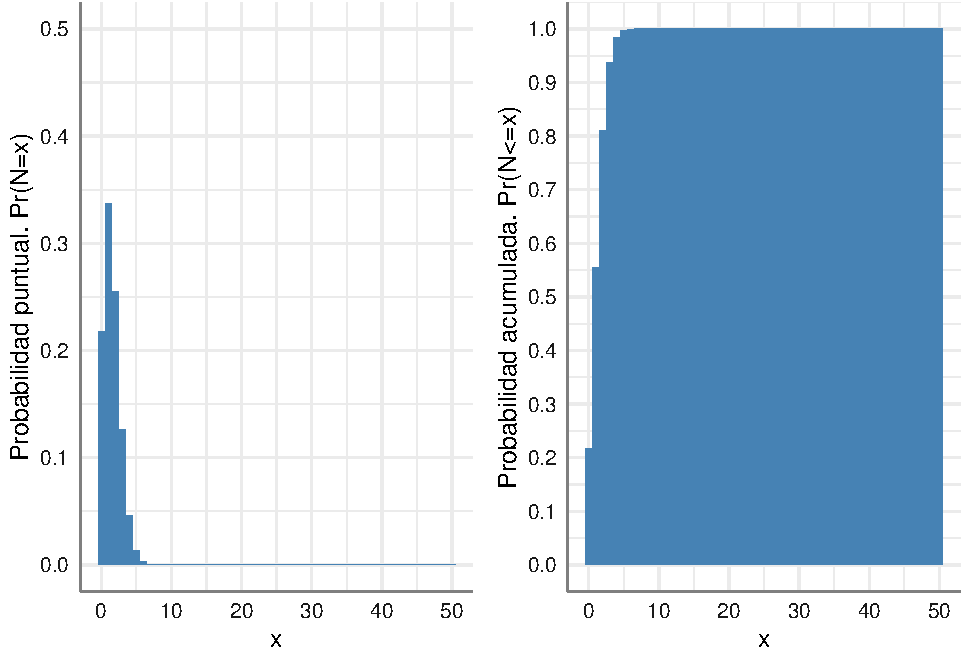
\includegraphics[width=0.95\linewidth]{01-Probabilidad_files/figure-latex/01-005-1} 

}

\caption{Función de masa de probabilidad y Función de distribución para el número de trabajadores de baja un día cualquiera.}\label{fig:01-005}
\end{figure}

En la fmp (Figura \ref{fig:01-005}-izquierda) podemos ver que en este caso la probabilidad se concentra en muy pocos valores, en concreto por debajo de 10, de modo que antes de llegar a \(x=10\) la probabilidad acumulada llega al valor 1, como se aprecia en la Figura \ref{fig:01-005}-derecha.

La probabilidad que nos reclaman en el enunciado es \[Pr(N\geq 3)=1-Pr(N \leq 2),\] que calculamos y podemos aproximar por MC a partir, por ejemplo, de 1000 simulaciones.

\begin{Shaded}
\begin{Highlighting}[]
\NormalTok{nsim}\OtherTok{=}\DecValTok{1000}
\NormalTok{n}\OtherTok{=}\DecValTok{50}
\NormalTok{p}\OtherTok{=}\FloatTok{0.03}
\CommentTok{\# valor real de la probabilidad}
\NormalTok{prob}\OtherTok{=}\DecValTok{1}\SpecialCharTok{{-}}\FunctionTok{pbinom}\NormalTok{(}\DecValTok{2}\NormalTok{,n,p)}
\FunctionTok{cat}\NormalTok{(}\StringTok{"Pr(N\textgreater{}=3)="}\NormalTok{,}\FunctionTok{round}\NormalTok{(prob,}\DecValTok{3}\NormalTok{))}
\end{Highlighting}
\end{Shaded}

\begin{verbatim}
## Pr(N>=3)= 0.189
\end{verbatim}

\begin{Shaded}
\begin{Highlighting}[]
\FunctionTok{set.seed}\NormalTok{(}\DecValTok{1234}\NormalTok{)}
\CommentTok{\# simulaciones}
\NormalTok{I.a}\OtherTok{=}\NormalTok{(}\FunctionTok{rbinom}\NormalTok{(nsim,n,p)}\SpecialCharTok{\textgreater{}=}\DecValTok{3}\NormalTok{)}\SpecialCharTok{*}\DecValTok{1}  \CommentTok{\# función indicatriz para la probabilidad requerida}
\NormalTok{prob}\OtherTok{=}\FunctionTok{mean}\NormalTok{(I.a)}
\FunctionTok{cat}\NormalTok{(}\StringTok{"AproxMC="}\NormalTok{,prob)}
\end{Highlighting}
\end{Shaded}

\begin{verbatim}
## AproxMC= 0.193
\end{verbatim}

El error estimado de esta aproximación, que calculamos con la raíz cuadrada de \eqref{eq:varianzaMC} es

\begin{Shaded}
\begin{Highlighting}[]
\NormalTok{error}\OtherTok{=}\FunctionTok{sqrt}\NormalTok{(}\FunctionTok{sum}\NormalTok{((I.a}\SpecialCharTok{{-}}\NormalTok{prob)}\SpecialCharTok{\^{}}\DecValTok{2}\NormalTok{)}\SpecialCharTok{/}\NormalTok{(nsim}\SpecialCharTok{\^{}}\DecValTok{2}\NormalTok{))}
\FunctionTok{cat}\NormalTok{(}\StringTok{"Error.AproxMC="}\NormalTok{,}\FunctionTok{round}\NormalTok{(error,}\DecValTok{3}\NormalTok{))}
\end{Highlighting}
\end{Shaded}

\begin{verbatim}
## Error.AproxMC= 0.012
\end{verbatim}

de donde podríamos calcular un intervalo de confianza para la aproximación MC de \(Pr(N \geq 3)\) al 95\% utilizando la distribución \eqref{eq:distMC} y la fórmula \eqref{eq:icMC}:

\begin{Shaded}
\begin{Highlighting}[]
\CommentTok{\# límites del IC redondeados a 3 cifras decimales}
\NormalTok{ic.low}\OtherTok{=}\FunctionTok{round}\NormalTok{(prob}\SpecialCharTok{{-}}\FunctionTok{qnorm}\NormalTok{(}\FloatTok{0.975}\NormalTok{)}\SpecialCharTok{*}\NormalTok{error,}\DecValTok{3}\NormalTok{)}
\NormalTok{ic.up}\OtherTok{=}\FunctionTok{round}\NormalTok{(prob}\SpecialCharTok{+}\FunctionTok{qnorm}\NormalTok{(}\FloatTok{0.975}\NormalTok{)}\SpecialCharTok{*}\NormalTok{error,}\DecValTok{3}\NormalTok{)}
\FunctionTok{cat}\NormalTok{(}\StringTok{"IC(95\%)[AproxMC]=["}\NormalTok{,ic.low,}\StringTok{","}\NormalTok{,ic.up,}\StringTok{"]"}\NormalTok{)}
\end{Highlighting}
\end{Shaded}

\begin{verbatim}
## IC(95%)[AproxMC]=[ 0.169 , 0.217 ]
\end{verbatim}

\end{example}

\begin{example}
\protect\hypertarget{exm:binom02}{}\label{exm:binom02}Una empresa de fabricación produce piezas, de las cuales el 97\% están dentro de las especificaciones y el 3\% son defectuosas (fuera de las especificaciones). Aparentemente no hay ningún patrón en la producción de piezas defectuosas. La cadena de producción empaqueta las piezas en cajas de 20 piezas cada una, y produce 1000 cajas al día. Al gerente de la empresa le gustaría estimar el número de cajas con al menos dos piezas defectuosas, de entre todas las que se producen al día durante un día cualquiera.
\end{example}

Si \(N\) es la variable aleatoria que recoge el número de piezas defectuosas en una caja, tenemos que:

\[N \sim Bi(20, 0.03)\]

La probabilidad de que una caja tenga al menos dos piezas defectuosas se calcula con \(p_N=Pr(N \geq 2)=1-Pr(N\leq 1)\).

\begin{Shaded}
\begin{Highlighting}[]
\NormalTok{n}\OtherTok{=}\DecValTok{20}
\NormalTok{p}\OtherTok{=}\FloatTok{0.03}
\NormalTok{prob}\OtherTok{=}\NormalTok{(}\DecValTok{1} \SpecialCharTok{{-}} \FunctionTok{pbinom}\NormalTok{(}\DecValTok{1}\NormalTok{, n,p))}
\FunctionTok{cat}\NormalTok{(}\StringTok{"Probabilidad de que una caja tenga al menos dos defectos="}\NormalTok{,prob)}
\end{Highlighting}
\end{Shaded}

\begin{verbatim}
## Probabilidad de que una caja tenga al menos dos defectos= 0.119838
\end{verbatim}

Sin embargo, lo que nos piden es, de un total de 1000 cajas, cuál es el número esperado de cajas con al meos dos piezas defectuosas. Para ello, surge la variable \(D_N\) que representa el número de cajas, de un total de 1000, con al menos 2 piezas defectuosas, que es binomial de tamaño 1000 y probabilidad \(p_N\),

\[D_N \sim Bin(1000,p_N),\]

y lo que nos están pidiendo es \(E(D_N)=1000 p_N\).

Si simulamos con la distribución de \(N\) lo acontecido un día, esto es, con 1000 cajas o simulaciones, y contamos el número de cajas con 2 o más piezas defectuosas, obtenemos una aproximación a la cantidad que nos piden.

\begin{Shaded}
\begin{Highlighting}[]
\NormalTok{n}\OtherTok{=}\DecValTok{20}
\NormalTok{p}\OtherTok{=}\FloatTok{0.03}
\FunctionTok{sum}\NormalTok{(}\FunctionTok{rbinom}\NormalTok{(}\DecValTok{1000}\NormalTok{,n,p)}\SpecialCharTok{\textgreater{}=}\DecValTok{2}\NormalTok{)}
\end{Highlighting}
\end{Shaded}

\begin{verbatim}
## [1] 99
\end{verbatim}

El problema es que no todos los días son iguales. De hecho si repites los siguientes cálculos varias veces, verás como el resultado varía. La aproximación Monte Carlo habría de considerar simulaciones de la variable \(D_n\) , esto es, \texttt{nsim} días, para con ellos poder sacar una conclusión ``promedio'' de lo que puede ocurrir un día cualquiera.

\begin{Shaded}
\begin{Highlighting}[]
\NormalTok{nsim}\OtherTok{=}\DecValTok{5000} \CommentTok{\# número de días simulados}
\NormalTok{n}\OtherTok{=}\DecValTok{1000}
\NormalTok{p}\OtherTok{=}\NormalTok{prob}
\CommentTok{\# valor real del valor esperado}
\NormalTok{media}\OtherTok{=}\NormalTok{n}\SpecialCharTok{*}\NormalTok{p}
\FunctionTok{cat}\NormalTok{(}\StringTok{"E(D\_N)="}\NormalTok{,}\FunctionTok{round}\NormalTok{(media,}\DecValTok{3}\NormalTok{))}
\end{Highlighting}
\end{Shaded}

\begin{verbatim}
## E(D_N)= 119.838
\end{verbatim}

\begin{Shaded}
\begin{Highlighting}[]
\CommentTok{\# simulaciones}
\NormalTok{xi}\OtherTok{=}\FunctionTok{rbinom}\NormalTok{(nsim,n,p)}
\NormalTok{m}\OtherTok{=}\FunctionTok{mean}\NormalTok{(}\FunctionTok{rbinom}\NormalTok{(nsim,n,p))}
\FunctionTok{cat}\NormalTok{(}\StringTok{"AproxMC="}\NormalTok{,m)}
\end{Highlighting}
\end{Shaded}

\begin{verbatim}
## AproxMC= 119.7926
\end{verbatim}

\begin{Shaded}
\begin{Highlighting}[]
\CommentTok{\# Error MC}
\NormalTok{error}\OtherTok{=}\FunctionTok{sqrt}\NormalTok{(}\FunctionTok{sum}\NormalTok{((xi}\SpecialCharTok{{-}}\NormalTok{m)}\SpecialCharTok{\^{}}\DecValTok{2}\NormalTok{)}\SpecialCharTok{/}\NormalTok{(nsim}\SpecialCharTok{\^{}}\DecValTok{2}\NormalTok{))}
\CommentTok{\# límites del IC redondeados a 3 cifras decimales}
\NormalTok{ic.low}\OtherTok{=}\FunctionTok{round}\NormalTok{(m}\SpecialCharTok{{-}}\FunctionTok{qnorm}\NormalTok{(}\FloatTok{0.975}\NormalTok{)}\SpecialCharTok{*}\NormalTok{error,}\DecValTok{3}\NormalTok{)}
\NormalTok{ic.up}\OtherTok{=}\FunctionTok{round}\NormalTok{(m}\SpecialCharTok{+}\FunctionTok{qnorm}\NormalTok{(}\FloatTok{0.975}\NormalTok{)}\SpecialCharTok{*}\NormalTok{error,}\DecValTok{3}\NormalTok{)}
\FunctionTok{cat}\NormalTok{(}\StringTok{"IC(95\%)[AproxMC]=["}\NormalTok{,ic.low,}\StringTok{","}\NormalTok{,ic.up,}\StringTok{"]"}\NormalTok{)}
\end{Highlighting}
\end{Shaded}

\begin{verbatim}
## IC(95%)[AproxMC]=[ 119.51 , 120.076 ]
\end{verbatim}

\hypertarget{geomuxe9trica}{%
\subsection{Geométrica}\label{geomuxe9trica}}

Imaginemos una situación experimental donde se repite un experimento hasta que sucede un ``éxito''. En otras palabras, se piensa en \(\theta\) como la probabilidad de éxito para un solo ensayo, y realizamos sucesivamente los ensayos hasta que se produce un éxito. La variable aleatoria \(N\) se define entonces como el número de ensayos Bernouilli realizados hasta conseguir un éxito. Nótese que aunque la variable aleatoria geométrica es discreta, su rango es infinito, y su fmp viene dada por:

\begin{equation}
Pr(N = x) = \theta (1-\theta)^{x}  \text{ para } x = \text{1, 2,...}
\label{eq:var-geometrica}
\end{equation}

con \(x\) el número de repeticiones hasta alcanzar un éxito, y \(\theta\) la probabilidad de éxito.

\begin{yellowbox}

\begin{definition}
\protect\hypertarget{def:vgeom}{}{\label{def:vgeom} }La variable aleatoria \(N\) cuya función de masa de probabilidad viene dada en \eqref{eq:var-geometrica} se denomina variable Geométrica de parámetro \(\theta\), y se denota por:

\[N \sim Ge(\theta)\]

con \(E(N) = \frac{1 - \theta}{\theta}\) y \(V(N) = \frac{1-\theta}{\theta^2}.\)\\
\end{definition}

\end{yellowbox}

Las funciones de \texttt{R} relacionadas con esta distribución se presentan a continuación, y tras ello un ejemplo de aplicación de la variable Geométrica.

\begin{whitebox}

\begin{itemize}
\tightlist
\item
  La función \texttt{dgeom(x,\ prob)} nos permite evaluar la \(Pr(N=x)\) para una variable Geométrica con probabilidad de éxito \texttt{prob}.
\item
  \texttt{pgeom(x,\ prob)} calcula la función de distribución.
\item
  \texttt{rgeom(n,\ prob)} permite generar \(n\) valores de una variable Geométrica con probabilidad de éxito \(prob\). Los resultados que proporciona son el número de repeticiones realizadas hasta alcanzar el primer éxito.
\end{itemize}

\end{whitebox}

\begin{example}
\protect\hypertarget{exm:geom01}{}\label{exm:geom01}Una vendedora de coches ha hecho un análisis estadístico de su historial de ventas anterior y ha determinado que cada día tiene un 10\% de probabilidad de vender un coche de lujo. Tras un cuidadoso análisis posterior, también está claro que la venta de un coche de lujo en un día es independiente de la ventas realizadas cualquier otro día. El día de Año Nuevo (un día festivo en el que el concesionario estaba cerrado) la vendedora está intentando predecir cuándo venderá su primer coche de lujo del año.
\end{example}

Si consideramos \(N\) como la variable aleatoria que indica el día de la primera venta de coches de lujo (N = 1 implica que la venta se realizaría el día 2 de enero), entonces:

\[N \sim Ge(0.1)\]

En este caso el valor esperado del número de días transcurridos hasta la venta del primer coche de lujo es \(E(N) = 0.9/0.1 = 9\) días, con una desviación típica de 9.5 días. Así pues, es posible que el día 10 de enero tenga su primera venta. En la Figura \ref{fig:01-008} se muestran la fmp y la función de distribución asociadas.

\begin{Shaded}
\begin{Highlighting}[]
\CommentTok{\# Valores de N}
\NormalTok{xs }\OtherTok{\textless{}{-}} \FunctionTok{seq}\NormalTok{(}\DecValTok{0}\NormalTok{, }\DecValTok{60}\NormalTok{, }\DecValTok{1}\NormalTok{)}
\CommentTok{\# Data frame}
\NormalTok{datos }\OtherTok{\textless{}{-}} \FunctionTok{data.frame}\NormalTok{(}\AttributeTok{xs =}\NormalTok{ xs, }\AttributeTok{probs =} \FunctionTok{dgeom}\NormalTok{(xs, }\FloatTok{0.1}\NormalTok{), }
                    \AttributeTok{probsacum =} \FunctionTok{pgeom}\NormalTok{(xs, }\FloatTok{0.1}\NormalTok{))}
\CommentTok{\# función de masa de probabilidad}
\NormalTok{g1 }\OtherTok{\textless{}{-}} \FunctionTok{ggplot}\NormalTok{(datos, }\FunctionTok{aes}\NormalTok{(xs, probs)) }\SpecialCharTok{+} 
  \FunctionTok{geom\_bar}\NormalTok{(}\AttributeTok{stat =} \StringTok{"identity"}\NormalTok{, }\AttributeTok{fill =} \StringTok{"steelblue"}\NormalTok{) }\SpecialCharTok{+}
  \FunctionTok{ylim}\NormalTok{(}\DecValTok{0}\NormalTok{,}\FloatTok{0.12}\NormalTok{) }\SpecialCharTok{+}
  \FunctionTok{labs}\NormalTok{(}\AttributeTok{x =}\StringTok{"x"}\NormalTok{, }\AttributeTok{y =} \StringTok{"Probabilidad puntual. Pr(N=x)"}\NormalTok{)}
\CommentTok{\# función de distribución}
\NormalTok{g2 }\OtherTok{\textless{}{-}} \FunctionTok{ggplot}\NormalTok{(datos, }\FunctionTok{aes}\NormalTok{(xs, probsacum)) }\SpecialCharTok{+} 
  \FunctionTok{geom\_bar}\NormalTok{(}\AttributeTok{stat =} \StringTok{"identity"}\NormalTok{, }\AttributeTok{fill =} \StringTok{"steelblue"}\NormalTok{) }\SpecialCharTok{+}
  \FunctionTok{scale\_y\_continuous}\NormalTok{(}\AttributeTok{breaks =}\NormalTok{ scales}\SpecialCharTok{::}\FunctionTok{breaks\_extended}\NormalTok{(}\DecValTok{10}\NormalTok{)) }\SpecialCharTok{+}
  \FunctionTok{labs}\NormalTok{(}\AttributeTok{x =}\StringTok{"x"}\NormalTok{, }\AttributeTok{y =} \StringTok{"Probabilidad acumulada Pr(N\textless{}=x)"}\NormalTok{)}
\FunctionTok{grid.arrange}\NormalTok{(g1, g2, }\AttributeTok{nrow =} \DecValTok{1}\NormalTok{)}
\end{Highlighting}
\end{Shaded}

\begin{figure}

{\centering 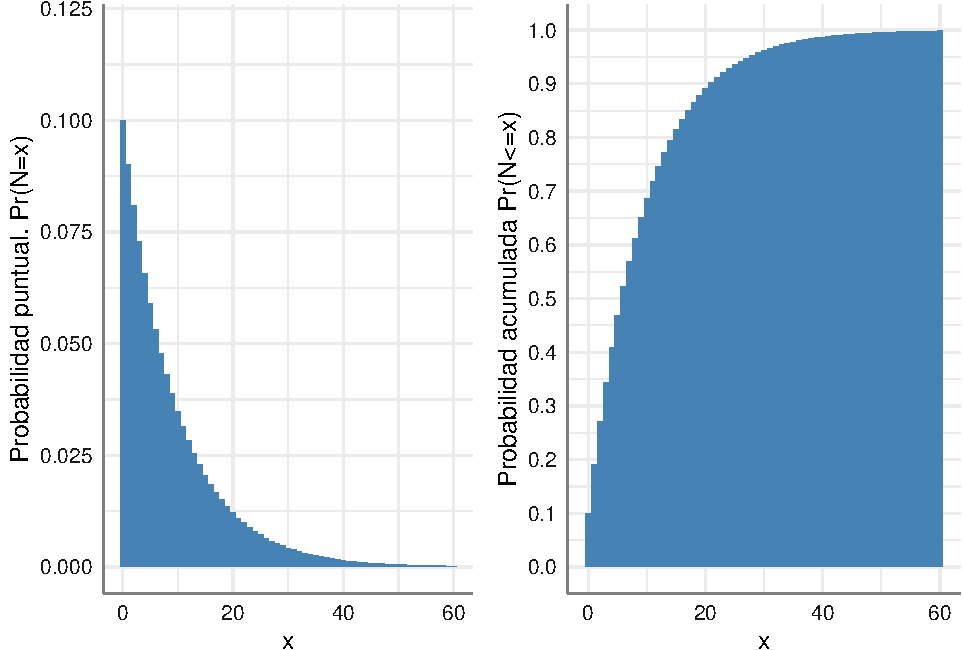
\includegraphics[width=0.95\linewidth]{01-Probabilidad_files/figure-latex/01-008-1} 

}

\caption{Función de masa de probabilidad y Función de distribución para el día en que venderá el primer coche de lujo.}\label{fig:01-008}
\end{figure}

Hacemos a continuación un análisis de simulación para aproximar los datos teóricos dados en la definición \ref{def:vgeom}. Simulamos 1000 valores de una \(Ge(0.1)\), con los que calculamos una aproximación al valor esperado de los días que deben transcurrir para vender un coche de lujo, y construimos un intervalo de confianza para la aproximación MC según \eqref{eq:icMC}.

\begin{Shaded}
\begin{Highlighting}[]
\CommentTok{\# Parámetros de la simulación}

\FunctionTok{set.seed}\NormalTok{(}\DecValTok{1970}\NormalTok{)}
\NormalTok{nsim }\OtherTok{\textless{}{-}} \DecValTok{10000}
\NormalTok{prob }\OtherTok{\textless{}{-}} \FloatTok{0.1}
\NormalTok{media}\OtherTok{\textless{}{-}}\NormalTok{(}\DecValTok{1}\SpecialCharTok{{-}}\NormalTok{prob)}\SpecialCharTok{/}\NormalTok{prob}
\FunctionTok{cat}\NormalTok{(}\StringTok{"E(N)="}\NormalTok{,media)}
\end{Highlighting}
\end{Shaded}

\begin{verbatim}
## E(N)= 9
\end{verbatim}

\begin{Shaded}
\begin{Highlighting}[]
\CommentTok{\# Valores simulados}
\NormalTok{datos }\OtherTok{\textless{}{-}} \FunctionTok{rgeom}\NormalTok{(nsim, prob)}
\CommentTok{\# Aproximación MC del valor esperado}
\NormalTok{m}\OtherTok{=}\FunctionTok{round}\NormalTok{(}\FunctionTok{mean}\NormalTok{(datos),}\DecValTok{0}\NormalTok{)}
\FunctionTok{cat}\NormalTok{(}\StringTok{"AproxMC="}\NormalTok{,m)}
\end{Highlighting}
\end{Shaded}

\begin{verbatim}
## AproxMC= 9
\end{verbatim}

\begin{Shaded}
\begin{Highlighting}[]
\CommentTok{\# Error MC}
\NormalTok{error}\OtherTok{=}\FunctionTok{sqrt}\NormalTok{(}\FunctionTok{sum}\NormalTok{((datos}\SpecialCharTok{{-}}\NormalTok{m)}\SpecialCharTok{\^{}}\DecValTok{2}\NormalTok{)}\SpecialCharTok{/}\NormalTok{(nsim}\SpecialCharTok{\^{}}\DecValTok{2}\NormalTok{))}
\CommentTok{\# límites del IC redondeados a 3 cifras decimales}
\NormalTok{ic.low}\OtherTok{=}\FunctionTok{round}\NormalTok{(m}\SpecialCharTok{{-}}\FunctionTok{qnorm}\NormalTok{(}\FloatTok{0.975}\NormalTok{)}\SpecialCharTok{*}\NormalTok{error,}\DecValTok{3}\NormalTok{)}
\NormalTok{ic.up}\OtherTok{=}\FunctionTok{round}\NormalTok{(m}\SpecialCharTok{+}\FunctionTok{qnorm}\NormalTok{(}\FloatTok{0.975}\NormalTok{)}\SpecialCharTok{*}\NormalTok{error,}\DecValTok{3}\NormalTok{)}
\FunctionTok{cat}\NormalTok{(}\StringTok{"IC(95\%)[AproxMC]=["}\NormalTok{,ic.low,}\StringTok{","}\NormalTok{,ic.up,}\StringTok{"]"}\NormalTok{)}
\end{Highlighting}
\end{Shaded}

\begin{verbatim}
## IC(95%)[AproxMC]=[ 8.811 , 9.189 ]
\end{verbatim}

\hypertarget{poisson}{%
\subsection{Poisson}\label{poisson}}

La distribución de Poisson se emplea como un modelo para variables aleatorias de tipo discreto cuando se quieren obtener las probabilidades de ocurrencia de un evento que se distribuye al azar en el espacio o el tiempo. Algunos ejemplos de esta distribución se presentan a continuación.

\begin{itemize}
\item
  En el estudio de cierto organismo acuático, se toman un gran número de muestras de un lago y se cuenta el número de dichos organismos que aparecen en cada muestra. Podríamos plantear como objetivo el conocer cuál es la probabilidad de encontrar dicho organismo en una próxima muestra si la media observada en el conjunto de muestras es de 2 organismos.
\item
  En un estudio sobre la efectividad de un insecticida sobre cierto tipo de insecto, se fumiga una gran región. Posteriormente se crea una cuadrícula sobre el terreno, se selecciona de forma aleatoria un conjunto de ellas, y se cuenta el número de insectos vivos dentro de cada una. Planteamos como objetivo conocer cuál es la probabilidad de que no encontremos ningún insecto vivo en una próxima cuadrícula si se sabe que la media de insectos vivos en las cuadrículas analizadas es de 0.5.
\item
  Un grupo de investigadores observó la ocurrencia de hemangioma capilar retiniano (RCH) en pacientes con la enfermedad de von Hippel-Lindau (VHL). RCH es un tumor vascular benigno de la retina. Usando una revisión retrospectiva de series de casos consecutivos, los investigadores encontraron que el número de medio de tumores RCH por ojo para pacientes con VHL era de 4. Están interesados en conocer cuál es la probabilidad de que se detecten más de cuatro tumores por ojo.
\end{itemize}

La variable aleatoria \(N\) se define entonces como el número de eventos que ocurren en un espacio o un tiempo determinados, y viene caracterizada por la denominada \emph{tasa de eventos} o \emph{número medio de eventos} que ocurren en el tiempo o espacio, y que se denota habitualmente por \(\lambda\). El rango de esta variable es infinito y su fmp viene dada por:

\begin{equation}
Pr(N = x) = \frac{e^{-\lambda}\lambda^x}{x!}  \text{ para } x = \text{1, 2,...}
\label{eq:var-poisson}
\end{equation}

con \(\lambda\) es la tasa y \(x\) es el número de eventos que han ocurrido.

\begin{yellowbox}

\begin{definition}
\protect\hypertarget{def:vpoisson}{}{\label{def:vpoisson} }La variable aleatoria \(X\) cuya función de masa de probabilidad viene dada en \eqref{eq:var-poisson} se denomina variable poisson de parámetro \(\lambda > 0\), y se denota por:

\[N \sim Po(\lambda)\]

con \(E(N) = \lambda\) y \(V(N) = \lambda.\)\\
\end{definition}

\end{yellowbox}

A continuación vemos diferentes ejemplos de uso de la distribución de Poisson, tras presentar las funciones de \texttt{R} relacionadas.

\begin{whitebox}

\begin{itemize}
\tightlist
\item
  La función \texttt{dpois(x,\ lambda)} nos permite evaluar la \(Pr(X=x)\) para una variable poisson de media \(\lambda\).
\item
  \texttt{ppois(x,\ lambda)} calcula la función de distribución.
\item
  \texttt{rpois(n,\ lambda)} permite generar \(n\) valores de una variable Poisson con media \(\lambda\). Los resultados que proporciona son el número de eventos que ocurren en el tiempo o espacio determinado.
\end{itemize}

\end{whitebox}

\begin{example}
\protect\hypertarget{exm:poisson01}{}\label{exm:poisson01}Una empresa de asesoramiento está realizando el análisis del funcionamiento de una panadería y ha estimado que el número medio de barras de pan que se venden en un periodo de media hora es de 12. La empresa está interesada en saber cuál es la capacidad de venta en cada franja de diez minutos (pues es prácticamente el tiempo de horneado), y también cuál es la probabilidad de que el número de barras que se venden en diez minutos sea exactamente de tres.
\end{example}

Como nuestro interés radica en un periodo de diez minutos y el número de intervalos de diez minutos en un periodo de 30 minutos es tres, tenemos que el número medio de barras puestas a la venta en ese periodo viene dado por:

\[\lambda = 12/3 = 4.\]

La variable aleatoria que reproduce el número de barras que se venden en una franja de cinco minutos es:

\[N \sim Po(4)\]

En este caso el valor esperado del número de barras que se venden es 4 y la desviación típica es igual a 2(\(=\sqrt{4}\)). En la Figura \ref{fig:01-010} se muestran la fmp y la función de distribución asociadas.

\begin{Shaded}
\begin{Highlighting}[]
\CommentTok{\# Valores de N}
\NormalTok{lambda}\OtherTok{=}\DecValTok{4}
\NormalTok{xs }\OtherTok{\textless{}{-}} \FunctionTok{seq}\NormalTok{(}\DecValTok{0}\NormalTok{, }\DecValTok{10}\NormalTok{, }\DecValTok{1}\NormalTok{)}
\CommentTok{\# Data frame}
\NormalTok{datos }\OtherTok{\textless{}{-}} \FunctionTok{data.frame}\NormalTok{(}\AttributeTok{xs =}\NormalTok{ xs, }\AttributeTok{probs =} \FunctionTok{dpois}\NormalTok{(xs, lambda), }
                    \AttributeTok{probsacum =} \FunctionTok{ppois}\NormalTok{(xs, lambda))}
\CommentTok{\# función de masa de probabilidad}
\NormalTok{g1 }\OtherTok{\textless{}{-}} \FunctionTok{ggplot}\NormalTok{(datos, }\FunctionTok{aes}\NormalTok{(xs, probs)) }\SpecialCharTok{+} 
  \FunctionTok{geom\_bar}\NormalTok{(}\AttributeTok{stat =} \StringTok{"identity"}\NormalTok{, }\AttributeTok{fill =} \StringTok{"steelblue"}\NormalTok{) }\SpecialCharTok{+}
  \FunctionTok{scale\_x\_continuous}\NormalTok{(}\AttributeTok{breaks =} \DecValTok{0}\SpecialCharTok{:}\DecValTok{10}\NormalTok{, }\AttributeTok{labels =} \DecValTok{0}\SpecialCharTok{:}\DecValTok{10}\NormalTok{) }\SpecialCharTok{+}
  \FunctionTok{ylim}\NormalTok{(}\DecValTok{0}\NormalTok{,}\FloatTok{0.3}\NormalTok{) }\SpecialCharTok{+}
  \FunctionTok{labs}\NormalTok{(}\AttributeTok{x =}\StringTok{"x"}\NormalTok{, }\AttributeTok{y =} \StringTok{"Probabilidad puntual. Pr(N=x)"}\NormalTok{)}
\CommentTok{\# función de distribución}
\NormalTok{g2 }\OtherTok{\textless{}{-}} \FunctionTok{ggplot}\NormalTok{(datos, }\FunctionTok{aes}\NormalTok{(xs, probsacum)) }\SpecialCharTok{+} 
  \FunctionTok{geom\_bar}\NormalTok{(}\AttributeTok{stat =} \StringTok{"identity"}\NormalTok{, }\AttributeTok{fill =} \StringTok{"steelblue"}\NormalTok{) }\SpecialCharTok{+}
  \FunctionTok{scale\_x\_continuous}\NormalTok{(}\AttributeTok{breaks =} \DecValTok{0}\SpecialCharTok{:}\DecValTok{10}\NormalTok{, }\AttributeTok{labels =} \DecValTok{0}\SpecialCharTok{:}\DecValTok{10}\NormalTok{) }\SpecialCharTok{+}
  \FunctionTok{scale\_y\_continuous}\NormalTok{(}\AttributeTok{breaks =}\NormalTok{ scales}\SpecialCharTok{::}\FunctionTok{breaks\_extended}\NormalTok{(}\DecValTok{10}\NormalTok{)) }\SpecialCharTok{+}
  \FunctionTok{labs}\NormalTok{(}\AttributeTok{x =}\StringTok{"x"}\NormalTok{, }\AttributeTok{y =} \StringTok{"Probabilidad acumulada Pr(N\textless{}=x)"}\NormalTok{)}
\FunctionTok{grid.arrange}\NormalTok{(g1, g2, }\AttributeTok{nrow =} \DecValTok{1}\NormalTok{)}
\end{Highlighting}
\end{Shaded}

\begin{figure}

{\centering 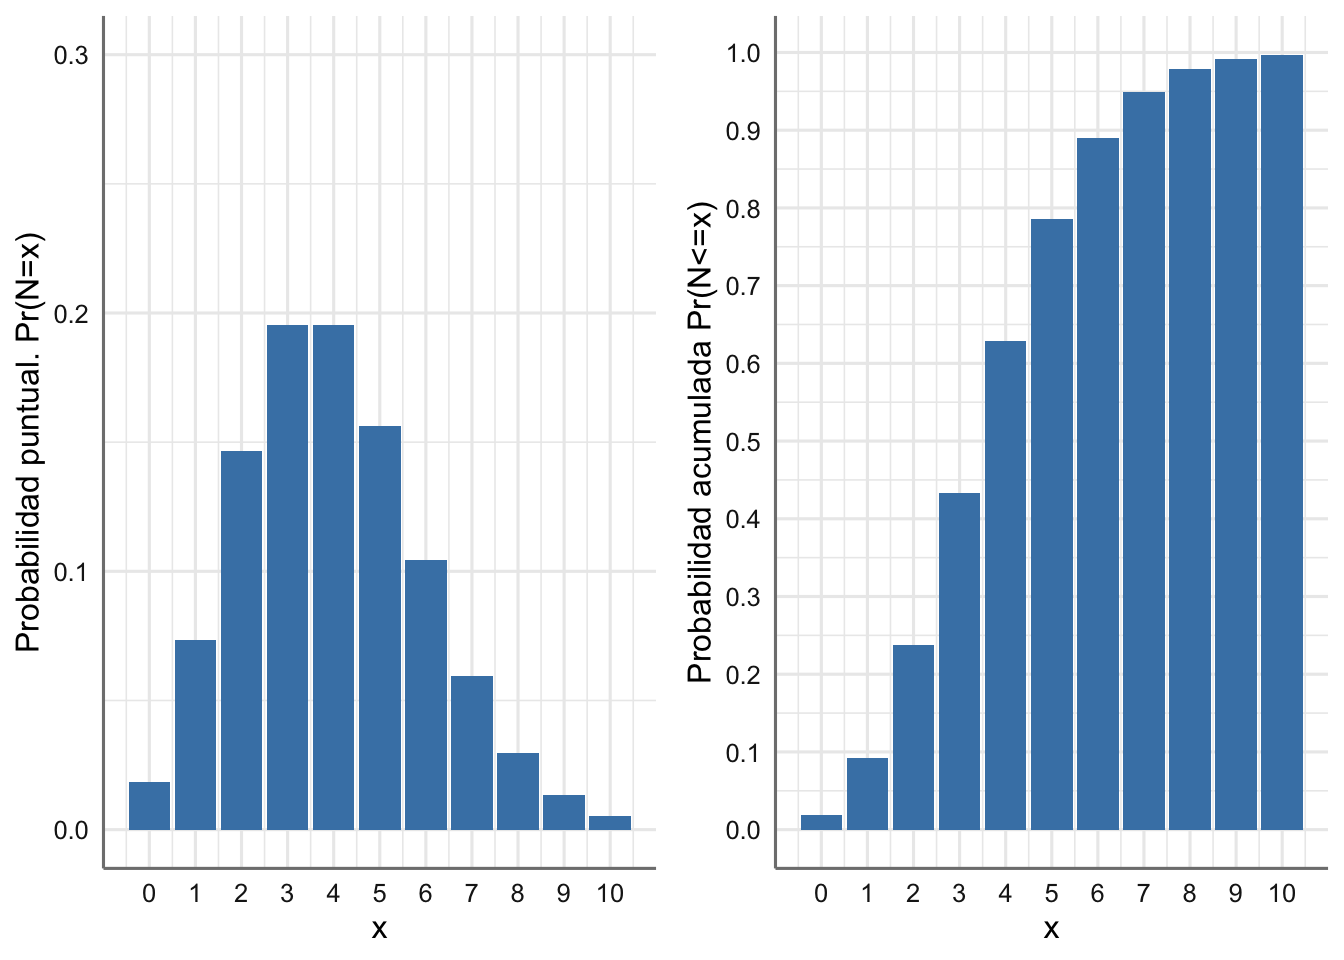
\includegraphics[width=0.95\linewidth]{01-Probabilidad_files/figure-latex/01-010-1} 

}

\caption{Función de masa de probabilidad y Función de distribución para el número de barras de pan que se venden cada cinco minutos.}\label{fig:01-010}
\end{figure}

Podemos reconoder en la Figura \ref{fig:01-010}-izquierda los valores más probables con las barras más altas (3 y 4). De hecho, en la Figura \ref{fig:01-010}-derecha, la probabilidad de que a lo sumo se vendan menos de 5 barras es algo superior a 0.6.

Para calcular la probabilidad pretendida, esto es, \(Pr(N=3)\) utilizamos la función fmp correspondiente en \texttt{R} y la aproximamos por MC con 1000 simulaciones, dando también una banda de confianza.

\begin{Shaded}
\begin{Highlighting}[]
\NormalTok{lambda}\OtherTok{=}\DecValTok{4}
\CommentTok{\# Probabilidad buscada P(N=3) para la poisson con media 2}
\NormalTok{media}\OtherTok{=}\FunctionTok{dpois}\NormalTok{(}\DecValTok{3}\NormalTok{,lambda)}
\FunctionTok{cat}\NormalTok{(}\StringTok{"Pr(N=4)="}\NormalTok{,}\FunctionTok{round}\NormalTok{(media,}\DecValTok{3}\NormalTok{))}
\end{Highlighting}
\end{Shaded}

\begin{verbatim}
## Pr(N=4)= 0.195
\end{verbatim}

\begin{Shaded}
\begin{Highlighting}[]
\NormalTok{nsim }\OtherTok{\textless{}{-}} \DecValTok{10000}
\CommentTok{\# Simulamos de la poisson y evaluamos la función indicatriz para la prob de interés}
\FunctionTok{set.seed}\NormalTok{(}\DecValTok{1970}\NormalTok{)}
\NormalTok{I.a }\OtherTok{\textless{}{-}}\NormalTok{ (}\FunctionTok{rpois}\NormalTok{(nsim, lambda)}\SpecialCharTok{==}\DecValTok{3}\NormalTok{)}\SpecialCharTok{*}\DecValTok{1}
\CommentTok{\# Realizamos la aproximación MC}
\NormalTok{m}\OtherTok{=}\FunctionTok{mean}\NormalTok{(I.a)}
\FunctionTok{cat}\NormalTok{(}\StringTok{"AproxMC="}\NormalTok{,m)}
\end{Highlighting}
\end{Shaded}

\begin{verbatim}
## AproxMC= 0.1934
\end{verbatim}

\begin{Shaded}
\begin{Highlighting}[]
\CommentTok{\# Error MC}
\NormalTok{error}\OtherTok{=}\FunctionTok{sqrt}\NormalTok{(}\FunctionTok{sum}\NormalTok{((I.a}\SpecialCharTok{{-}}\NormalTok{m)}\SpecialCharTok{\^{}}\DecValTok{2}\NormalTok{)}\SpecialCharTok{/}\NormalTok{(nsim}\SpecialCharTok{\^{}}\DecValTok{2}\NormalTok{))}
\CommentTok{\# límites del IC redondeados a 3 cifras decimales}
\NormalTok{ic.low}\OtherTok{=}\FunctionTok{round}\NormalTok{(m}\SpecialCharTok{{-}}\FunctionTok{qnorm}\NormalTok{(}\FloatTok{0.975}\NormalTok{)}\SpecialCharTok{*}\NormalTok{error,}\DecValTok{3}\NormalTok{)}
\NormalTok{ic.up}\OtherTok{=}\FunctionTok{round}\NormalTok{(m}\SpecialCharTok{+}\FunctionTok{qnorm}\NormalTok{(}\FloatTok{0.975}\NormalTok{)}\SpecialCharTok{*}\NormalTok{error,}\DecValTok{3}\NormalTok{)}
\FunctionTok{cat}\NormalTok{(}\StringTok{"IC(95\%)[AproxMC]=["}\NormalTok{,ic.low,}\StringTok{","}\NormalTok{,ic.up,}\StringTok{"]"}\NormalTok{)}
\end{Highlighting}
\end{Shaded}

\begin{verbatim}
## IC(95%)[AproxMC]=[ 0.186 , 0.201 ]
\end{verbatim}

Si la aproximación la hacemos con 10 veces más simulaciones, el intervalo de estimación resultará más preciso:

\begin{Shaded}
\begin{Highlighting}[]
\NormalTok{lambda}\OtherTok{=}\DecValTok{4}
\CommentTok{\# Probabilidad buscada P(N=3) para la poisson con media 2}
\NormalTok{media}\OtherTok{=}\FunctionTok{dpois}\NormalTok{(}\DecValTok{3}\NormalTok{,lambda)}
\FunctionTok{cat}\NormalTok{(}\StringTok{"Pr(N=4)="}\NormalTok{,}\FunctionTok{round}\NormalTok{(media,}\DecValTok{3}\NormalTok{))}
\end{Highlighting}
\end{Shaded}

\begin{verbatim}
## Pr(N=4)= 0.195
\end{verbatim}

\begin{Shaded}
\begin{Highlighting}[]
\NormalTok{nsim }\OtherTok{\textless{}{-}} \DecValTok{10000}\SpecialCharTok{*}\DecValTok{10}
\CommentTok{\# Simulamos de la poisson y evaluamos la función indicatriz para la prob de interés}
\FunctionTok{set.seed}\NormalTok{(}\DecValTok{1970}\NormalTok{)}
\NormalTok{I.a }\OtherTok{\textless{}{-}}\NormalTok{ (}\FunctionTok{rpois}\NormalTok{(nsim, lambda)}\SpecialCharTok{==}\DecValTok{3}\NormalTok{)}\SpecialCharTok{*}\DecValTok{1}
\CommentTok{\# Realizamos la aproximación MC}
\NormalTok{m}\OtherTok{=}\FunctionTok{mean}\NormalTok{(I.a)}
\FunctionTok{cat}\NormalTok{(}\StringTok{"AproxMC="}\NormalTok{,m)}
\end{Highlighting}
\end{Shaded}

\begin{verbatim}
## AproxMC= 0.19375
\end{verbatim}

\begin{Shaded}
\begin{Highlighting}[]
\CommentTok{\# Error MC}
\NormalTok{error}\OtherTok{=}\FunctionTok{sqrt}\NormalTok{(}\FunctionTok{sum}\NormalTok{((I.a}\SpecialCharTok{{-}}\NormalTok{m)}\SpecialCharTok{\^{}}\DecValTok{2}\NormalTok{)}\SpecialCharTok{/}\NormalTok{(nsim}\SpecialCharTok{\^{}}\DecValTok{2}\NormalTok{))}
\CommentTok{\# límites del IC redondeados a 3 cifras decimales}
\NormalTok{ic.low}\OtherTok{=}\FunctionTok{round}\NormalTok{(m}\SpecialCharTok{{-}}\FunctionTok{qnorm}\NormalTok{(}\FloatTok{0.975}\NormalTok{)}\SpecialCharTok{*}\NormalTok{error,}\DecValTok{3}\NormalTok{)}
\NormalTok{ic.up}\OtherTok{=}\FunctionTok{round}\NormalTok{(m}\SpecialCharTok{+}\FunctionTok{qnorm}\NormalTok{(}\FloatTok{0.975}\NormalTok{)}\SpecialCharTok{*}\NormalTok{error,}\DecValTok{3}\NormalTok{)}
\FunctionTok{cat}\NormalTok{(}\StringTok{"IC(95\%)[AproxMC]=["}\NormalTok{,ic.low,}\StringTok{","}\NormalTok{,ic.up,}\StringTok{"]"}\NormalTok{)}
\end{Highlighting}
\end{Shaded}

\begin{verbatim}
## IC(95%)[AproxMC]=[ 0.191 , 0.196 ]
\end{verbatim}

\begin{example}
\protect\hypertarget{exm:poisson02}{}\label{exm:poisson02}Una empresa de fabricación de galletas de chocolate está analizando la calidad en su empresa para responder del mejor modo posible a sus clientes. Para ello ha fijado que con probabilidad 0.8 las galletas deben contener al menos tres trozos de chocolate para satisfacer las exigencias de los clientes. Se trata pues de fijar el valor medio de trozos de chocolate que debe ir suministrando en la cadena de producción para cumplir con el nivel de exigencia establecido.
\end{example}

Si \(N\) es la variable aleatoria que indica el número de trozos de chocolate en una galleta, tenemos que:

\[N \sim Po(\lambda)\]

donde en este caso el valor de \(\lambda\) es desconocido y representa el número medio de trozos de chocolate en cada galleta. Planteamos un estudio de simulación para aproximar dicho valor.

\begin{silverbox}

Algoritmo para aproximar el valor de \(\lambda\).

\begin{enumerate}
\def\labelenumi{\arabic{enumi}.}
\tightlist
\item
  Considerar una secuencia de valores de \(\lambda_i\), \(i=1,...,K\)
\item
  Obtener una muestra de tamaño \(nsim\) para cada distribución \(Po(\lambda_i)\), \(M_i=\{x_{i_1},\ldots,x_{i_{nsim}}\}\).
\item
  Con cada muestra \(M_i\) aproximar la probabilidad de que el número de trozos sea mayor o igual a 3, \(p_i\approx Pr(N_{\lambda_i}\geq3)\).
\item
  Obtener el valor mínimo de \(\lambda\), de entre \(\{\lambda_1,\ldots,\lambda_K\}\) que verifica \(p_i \geq 0.8\).
\end{enumerate}

\end{silverbox}

En la Figura \ref{fig:01-013} se muestra el proceso de simulación realizado a continuación y el resultado obtenido para el valor de \(\lambda\) para cumplir los requisitos de la empresa.

\begin{Shaded}
\begin{Highlighting}[]
\CommentTok{\# Paso 1}
\FunctionTok{set.seed}\NormalTok{(}\DecValTok{1970}\NormalTok{)}
\NormalTok{nsim }\OtherTok{\textless{}{-}} \DecValTok{5000}
\NormalTok{lams }\OtherTok{\textless{}{-}} \FunctionTok{seq}\NormalTok{(}\FloatTok{0.1}\NormalTok{, }\DecValTok{5}\NormalTok{, }\FloatTok{0.01}\NormalTok{) }\CommentTok{\# valores de lambda}
\NormalTok{nlams }\OtherTok{\textless{}{-}} \FunctionTok{length}\NormalTok{(lams)     }\CommentTok{\# número de lambdas para evaluar}
\NormalTok{prob }\OtherTok{\textless{}{-}} \FunctionTok{c}\NormalTok{()  }\CommentTok{\# vector de probabilidades}

\CommentTok{\# Pasos 2 y 3}
\ControlFlowTok{for}\NormalTok{(i }\ControlFlowTok{in} \DecValTok{1}\SpecialCharTok{:}\NormalTok{nlams)\{}
\NormalTok{  datos }\OtherTok{\textless{}{-}} \FunctionTok{rpois}\NormalTok{(nsim, lams[i])    }
\NormalTok{  prob[i] }\OtherTok{\textless{}{-}} \FunctionTok{mean}\NormalTok{(datos }\SpecialCharTok{\textgreater{}=} \DecValTok{3}\NormalTok{)   }
\NormalTok{\}}

\CommentTok{\# Paso 4. Resultado del problema}
\NormalTok{lambda}\OtherTok{=}\NormalTok{lams[}\FunctionTok{min}\NormalTok{(}\FunctionTok{which}\NormalTok{(prob }\SpecialCharTok{\textgreater{}=} \FloatTok{0.8}\NormalTok{))];lambda}
\end{Highlighting}
\end{Shaded}

\begin{verbatim}
## [1] 4.25
\end{verbatim}

\begin{Shaded}
\begin{Highlighting}[]
\CommentTok{\# Pintamos los resultados de la simulación realizada}
\NormalTok{dat}\OtherTok{=}\FunctionTok{data.frame}\NormalTok{(}\AttributeTok{lams=}\NormalTok{lams,}\AttributeTok{prob=}\NormalTok{prob)}
\FunctionTok{ggplot}\NormalTok{(dat,}\FunctionTok{aes}\NormalTok{(}\AttributeTok{x=}\NormalTok{lams,}\AttributeTok{y=}\NormalTok{prob))}\SpecialCharTok{+}
  \FunctionTok{geom\_point}\NormalTok{()}\SpecialCharTok{+}
  \FunctionTok{geom\_hline}\NormalTok{(}\AttributeTok{yintercept=}\FloatTok{0.8}\NormalTok{)}\SpecialCharTok{+}
  \FunctionTok{geom\_vline}\NormalTok{(}\AttributeTok{xintercept=}\NormalTok{lambda)}\SpecialCharTok{+}
  \FunctionTok{labs}\NormalTok{(}\AttributeTok{x=}\StringTok{"lambda"}\NormalTok{,}\AttributeTok{y=}\StringTok{"Pr(N\textgreater{}=3)"}\NormalTok{)}
\end{Highlighting}
\end{Shaded}

\begin{figure}

{\centering 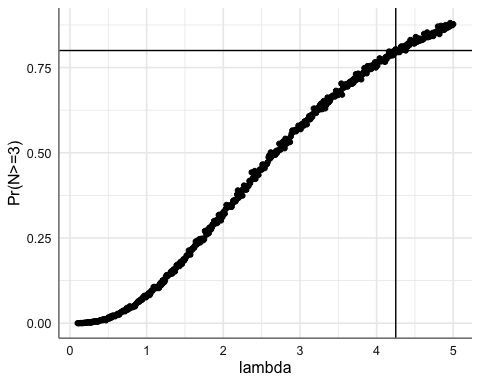
\includegraphics[width=0.95\linewidth]{01-Probabilidad_files/figure-latex/01-013-1} 

}

\caption{Probabilidad estimada de conseguir al menos 3 trozos de chocolate en cada galleta, en función de lambda.}\label{fig:01-013}
\end{figure}

Así pues, el número medio de trozos de chocolate que ha de suministrarse a cada galleta ha de ser al menos de 4.25.

\hypertarget{distribuciones-continuas}{%
\section{Distribuciones continuas}\label{distribuciones-continuas}}

En este punto estudiamos las principales variables de tipo continuo. La especificación de estas variables se hace a partir de la función de densidad.

\hypertarget{uniforme}{%
\subsection{Uniforme}\label{uniforme}}

La distribución uniforme es la distribución de probabilidad continua más sencilla y se refiere a eventos infinitos que tienen la misma probabilidad de ocurrir en una intervalo dado. Si \(a\) y \(b\) son dos números reales con \(a < b\) entonces la función de distribución asociada a la probabilidad acumulada a la izquierda de cualquier valor \(x \in [a, b]\) viene dada por:

\begin{equation}
F(x) = 
\begin{cases}
0 & \text{ si } x < a \\
\frac{x-a}{b-a} & \text{ si } a \leq x \leq b\\
1 & \text{ si } a \leq x \leq b.
\end{cases}
\label{eq:var-uniforme2}
\end{equation}

\begin{yellowbox}

\begin{definition}
\protect\hypertarget{def:vuniforme}{}{\label{def:vuniforme} }Una variable aleatoria \(X\) tiene una distribución uniforme en el intervalo \([a, b]\), con \$a,b \in R,

\[X \sim U(a,b)\]

si su función de densidad viene dada por la expresión

\begin{equation}
f(x) = 
\begin{cases}
\frac{1}{b-a} & \text{ si } a \leq x \leq b\\
0 & \text{ en otro caso }
\end{cases}
\label{eq:var-uniforme}
\end{equation}

de forma que \(E(X) = (a+b)/2\) y \(V(X) = (b-a)^2/12.\)\\
\end{definition}

\end{yellowbox}

La variable uniforme más famosa es la \(U(0,1)\) ya que se utiliza habitualmente para modelizar la incertidumbre sobre una probabilidad desconocida, y es la base para muchos de los algoritmos de simulación de variables y procesos que estudiaremos en el futuro.

\begin{whitebox}

\begin{itemize}
\tightlist
\item
  La función \texttt{runif(n,\ a,\ b)} permite generar \(n\) valores de una variable uniforme en el intervalo \([a, b]\); \texttt{runif(n)} da una muestra para una distribución uniforme en {[}0, 1{]}.
\item
  \texttt{dunif(x,a,b)} da la fdp en \(x\).
\item
  \texttt{punif(x,a,b)} da la probabilidad acumulada para cualquier punto \(x \in [a,b]\).
\end{itemize}

\end{whitebox}

\hypertarget{exponencial}{%
\subsection{Exponencial}\label{exponencial}}

La distribución exponencial es una distribución muy común en la modelización probabilística. Esta distribución describe procesos que describen el tiempo entre sucesos consecutivos, con la peculiaridad de que sus probabilidades no dependen del instante en que se produzcan los eventos. Es decir:

\[Pr(X > t+s | X > t) = Pr(X > s).\]

Esta propiedad es característica de la distribución exponencial y se denomina ``propiedad de la pérdida de memoria''.

Ejemplos de este tipo de distribución son:

\begin{itemize}
\item
  El tiempo que tarda una partícula radiactiva en desintegrarse. El conocimiento de la ley que sigue este evento se utiliza en ciencias para, por ejemplo, la datación de fósiles o cualquier materia orgánica mediante la técnica del carbono 14.
\item
  El tiempo que puede transcurrir en un servicio de urgencias, entre llegadas de pacientes, o en una fábrica entre roturas de una máquina.
\end{itemize}

Esta distribución está muy relacionada con unos procesos que estudiaremos más adelante, denominados Procesos de Poisson.

La distribución exponencial viene completamente especificada, a través del parámetro \(\lambda >0\) que mide el número esperado de veces que ocurre el evento de interés por cada unidad de tiempo, y cuya función de distribución viene dada por:

\begin{equation}
F(x) = 
\begin{cases}
0 & \text{ si } x < 0 \\
1 - e^{\lambda x} & \text{ si } x \geq 0.
\end{cases}
\label{eq:var-exponencial2}
\end{equation}

\begin{yellowbox}

\begin{definition}
\protect\hypertarget{def:vexponencial}{}\label{def:vexponencial}Una variable aleatoria \(X\) tiene una distribución exponencial de parámetro \(\lambda\), que se denota por

\[X \sim Exp(\lambda)\]

si su función de densidad viene dada por

\begin{equation}
f(x)=\lambda e^{-\lambda x}, \quad x \geq 0,
\end{equation}

de forma que \(E(X) = 1/\lambda\) y \(V(X) = 1/\lambda^2.\)
\end{definition}

\end{yellowbox}

Las funciones relacionadas con la distribución exponencial en \texttt{R} son:

\begin{whitebox}

\begin{itemize}
\tightlist
\item
  La función \texttt{dexp(x,\ lambda)} nos permite evaluar la función de densidad para una variable poisson de parámetro \(\lambda\).
\item
  \texttt{pexp(x,\ lambda)} nos permite evaluar la función de distribución.
\item
  \texttt{rexp(n,\ lambda)} permite generar \(n\) valores de una variable Exponencial de parámetro \(\lambda\).
\end{itemize}

\end{whitebox}

A continuación estudiamos dos ejemplos de uso de la distribución exponencial. Como siempre presentamos los resultados téoricos y procedemos mediante simulación para ver la aproximación conseguida.

\begin{example}
\protect\hypertarget{exm:exponencial01}{}\label{exm:exponencial01}Se ha comprobado que el tiempo de vida de cierto tipo de marcapasos sigue una distribución exponencial con media 16 años. (1) ¿Cuál es la probabilidad de que a una persona a la que se le ha implantado este marcapasos se le deba reimplantar otro antes de 20 años? (2) Si el marcapasos lleva funcionando correctamente 5 años en un paciente, ¿cuál es la probabilidad de que haya que cambiarlo antes de 25 años desde que se implantó?
\end{example}

Si \(T\) es la variable aleatoria que indica el tiempo de vida del marcapasos tenemos que:

\[T \sim Exp(\lambda = 1/16)\]

Se puede reponder fácilmente a las preguntas planteadas sin más que hacer uso de la función \texttt{pexp()}. Sin embargo, también simularemos para aproximarlas. Hemos de calcular

(1). Si es preciso implantar antes de 20 años, es porque el tiempo de vida no va a ser superior a 20. Hemos de calcular pues, \(Pr(T \leq 20)\). (2). Nos piden \(Pr(T \leq 25|T>5)=Pr(T\leq 20)\), por la propiedad de la pérdida de memoria. Es decir, respondiendo a (1) tendremos respondidas las dos preguntas formuladas.

\begin{Shaded}
\begin{Highlighting}[]
\NormalTok{lambda }\OtherTok{\textless{}{-}} \DecValTok{1}\SpecialCharTok{/}\DecValTok{16}
\CommentTok{\# Data frame para la representación gráfica}
\NormalTok{sec }\OtherTok{\textless{}{-}} \FunctionTok{seq}\NormalTok{(}\DecValTok{0}\NormalTok{, }\DecValTok{80}\NormalTok{, }\AttributeTok{by =} \FloatTok{0.01}\NormalTok{)}
\NormalTok{datos}\OtherTok{\textless{}{-}} \FunctionTok{data.frame}\NormalTok{(}\AttributeTok{sec =}\NormalTok{ sec, }\AttributeTok{densidad =} \FunctionTok{dexp}\NormalTok{(sec,lambda))}
\CommentTok{\# Gráfico función de densidad}
\FunctionTok{ggplot}\NormalTok{(datos, }\FunctionTok{aes}\NormalTok{(sec, densidad)) }\SpecialCharTok{+} 
  \FunctionTok{geom\_line}\NormalTok{() }\SpecialCharTok{+}
  \FunctionTok{scale\_x\_continuous}\NormalTok{(}\AttributeTok{breaks =} \FunctionTok{seq}\NormalTok{(}\DecValTok{0}\NormalTok{,}\DecValTok{80}\NormalTok{,}\DecValTok{5}\NormalTok{), }\AttributeTok{labels =} \FunctionTok{seq}\NormalTok{(}\DecValTok{0}\NormalTok{,}\DecValTok{80}\NormalTok{,}\DecValTok{5}\NormalTok{)) }\SpecialCharTok{+}
  \FunctionTok{scale\_y\_continuous}\NormalTok{(}\AttributeTok{breaks =}\NormalTok{ scales}\SpecialCharTok{::}\FunctionTok{breaks\_extended}\NormalTok{(}\DecValTok{10}\NormalTok{)) }\SpecialCharTok{+}
  \FunctionTok{geom\_vline}\NormalTok{(}\AttributeTok{xintercept =} \DecValTok{20}\NormalTok{, }\AttributeTok{col =} \StringTok{"red"}\NormalTok{) }\SpecialCharTok{+}
  \FunctionTok{labs}\NormalTok{(}\AttributeTok{x =}\StringTok{"Tiempo de vida del marcapasos (en años)"}\NormalTok{, }
       \AttributeTok{y =} \StringTok{"Función de densidad"}\NormalTok{)}
\end{Highlighting}
\end{Shaded}

\begin{figure}

{\centering 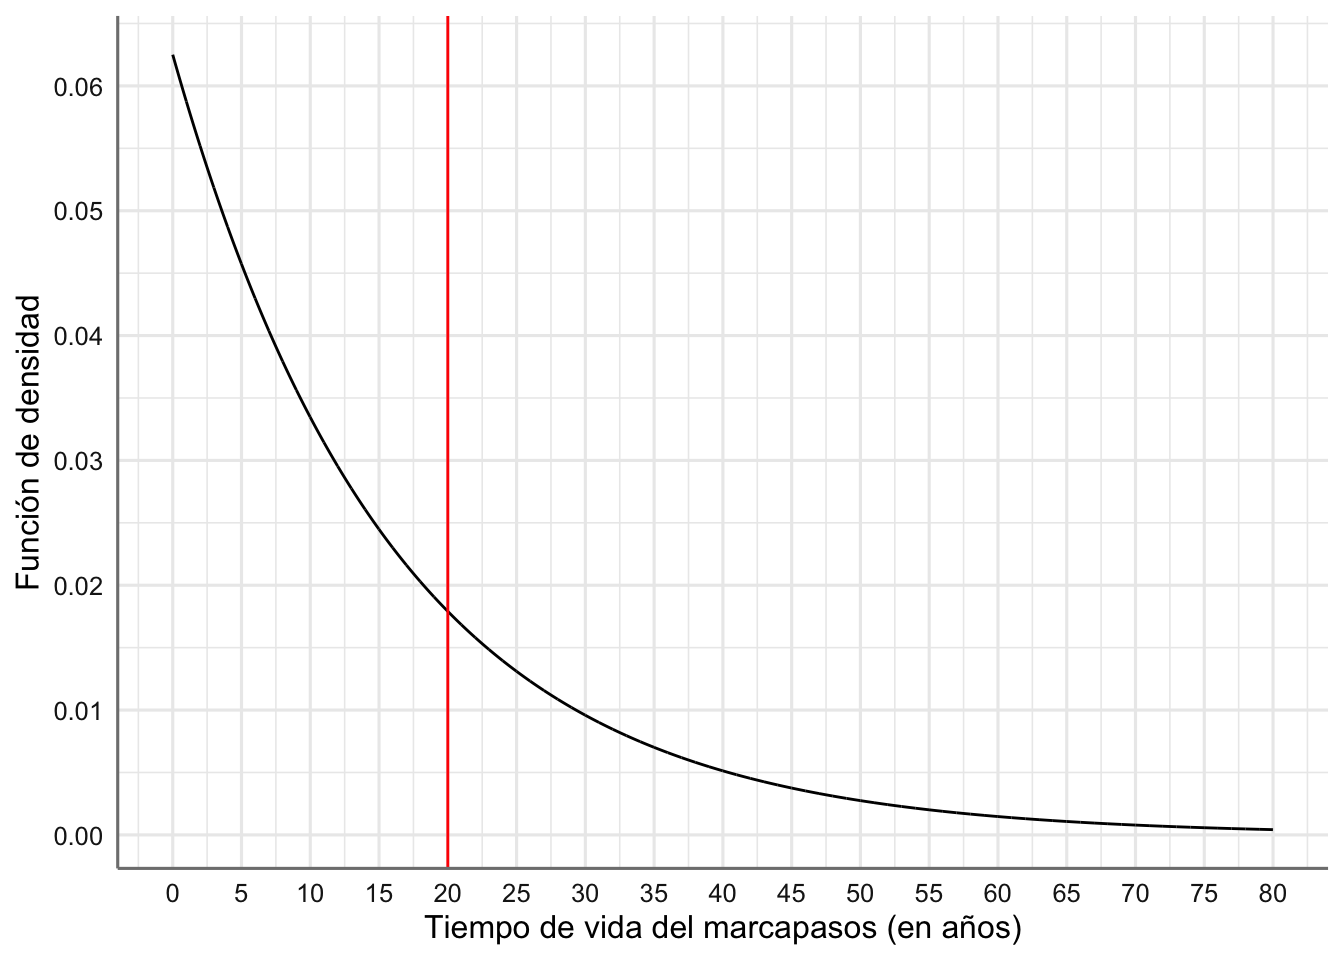
\includegraphics[width=0.95\linewidth]{01-Probabilidad_files/figure-latex/01-014-1} 

}

\caption{Función de densidad del tiempo de vida del marcapasos (en años)}\label{fig:01-014}
\end{figure}

Obtenemos la probabilidad deseada:

\begin{Shaded}
\begin{Highlighting}[]
\CommentTok{\# Probabilidad real}
\NormalTok{lambda}\OtherTok{=}\DecValTok{1}\SpecialCharTok{/}\DecValTok{16}
\NormalTok{p}\OtherTok{=}\FunctionTok{pexp}\NormalTok{(}\DecValTok{20}\NormalTok{,lambda)}
\FunctionTok{cat}\NormalTok{(}\StringTok{"Pr(T\textless{}=20)="}\NormalTok{,}\FunctionTok{round}\NormalTok{(p,}\DecValTok{3}\NormalTok{))}
\end{Highlighting}
\end{Shaded}

\begin{verbatim}
## Pr(T<=20)= 0.713
\end{verbatim}

\begin{Shaded}
\begin{Highlighting}[]
\CommentTok{\# Parámetros de la simulación}
\FunctionTok{set.seed}\NormalTok{(}\DecValTok{123}\NormalTok{)}
\NormalTok{nsim }\OtherTok{\textless{}{-}} \DecValTok{5000}
\CommentTok{\# Simulaciones}
\NormalTok{datos }\OtherTok{\textless{}{-}} \FunctionTok{rexp}\NormalTok{(nsim, lambda)}
\CommentTok{\# Probabilidad de interés}
\NormalTok{pMC}\OtherTok{=}\FunctionTok{mean}\NormalTok{(datos }\SpecialCharTok{\textless{}=} \DecValTok{20}\NormalTok{)}
\FunctionTok{cat}\NormalTok{(}\StringTok{"Aprox.MC[Pr(T\textless{}=20)]="}\NormalTok{,}\FunctionTok{round}\NormalTok{(pMC,}\DecValTok{3}\NormalTok{))}
\end{Highlighting}
\end{Shaded}

\begin{verbatim}
## Aprox.MC[Pr(T<=20)]= 0.711
\end{verbatim}

La probabilidad de que el marcapasos dure más de 20 años y haya que reemplazarlo es de 0.289, por lo que efectivamente, es muy recomendable reemplazarlo antes. Sin embargo, al paciente en la pregunta (2) se le daría la misma recomendación, cuando la probabilidad de que el marcapasos dure más de 25 años desde su implante, que sería el tiempo que lo llevaría, es considerablemente inferior, 0.21. No es pues recomendable, utilizar esta distribución para modelizar el tiempo de vida de un implante.

\begin{example}
\protect\hypertarget{exm:exponencial02}{}\label{exm:exponencial02}Un motor eléctrico tiene una vida media de 6 años y se modeliza con una distribución exponencial. ¿Cuál debe ser el tiempo de garantía que debe tener el motor si se desea que a lo sumo el 15 \% de los motores fallen antes de que expire su garantía?
\end{example}

Si \(T\) es la variable aleatoria que indica el tiempo de vida del producto tenemos que: \[T \sim Exp(\lambda = 1/6).\]\\
En este caso estamos interesados en encontrar el tiempo para que podamos garantizar que el 85\% de los motores siguen funcionando, es decir, buscamos el cuantil 0.15 de la distribución de \(T\). Planteamos un análisis de simulación para estimar dicho valor.

\begin{Shaded}
\begin{Highlighting}[]
\CommentTok{\# Calculamos el valor real para el periodo de garantía}
\NormalTok{lambda }\OtherTok{\textless{}{-}} \DecValTok{1}\SpecialCharTok{/}\DecValTok{6}
\NormalTok{q}\OtherTok{=}\FunctionTok{qexp}\NormalTok{(}\FloatTok{0.15}\NormalTok{,lambda)}
\FunctionTok{cat}\NormalTok{(}\StringTok{"Periodo de garantía recomendado="}\NormalTok{,}\FunctionTok{round}\NormalTok{(q,}\DecValTok{2}\NormalTok{))}
\end{Highlighting}
\end{Shaded}

\begin{verbatim}
## Periodo de garantía recomendado= 0.98
\end{verbatim}

\begin{Shaded}
\begin{Highlighting}[]
\CommentTok{\# Parámetros de la simulación}
\FunctionTok{set.seed}\NormalTok{(}\DecValTok{123}\NormalTok{)}
\NormalTok{nsim }\OtherTok{\textless{}{-}} \DecValTok{5000}
\CommentTok{\# simulaciones}
\NormalTok{datos }\OtherTok{\textless{}{-}} \FunctionTok{rexp}\NormalTok{(nsim, lambda)}
\CommentTok{\# cuantil de interés}
\NormalTok{qMC}\OtherTok{=}\FunctionTok{quantile}\NormalTok{(datos, }\FloatTok{0.15}\NormalTok{)}
\FunctionTok{cat}\NormalTok{(}\StringTok{"Periodo de garantía aproximado="}\NormalTok{,}\FunctionTok{round}\NormalTok{(qMC,}\DecValTok{2}\NormalTok{))}
\end{Highlighting}
\end{Shaded}

\begin{verbatim}
## Periodo de garantía aproximado= 1.02
\end{verbatim}

Para que tan sólo el 15\% de los motores necesiten reparación durante el periodo de garantía, debemos establecer una garantía de aproximadamente 1 año.

En la Figura \ref{fig:01-016-2} se representan, para los datos simulados, los cuantiles aproximados versus su probabilidad asociada. Con el gráfico se puede atisbar también el periodo de garantía recomendado.

\begin{Shaded}
\begin{Highlighting}[]
\CommentTok{\# cuantil de interés}
\NormalTok{probs }\OtherTok{\textless{}{-}} \FunctionTok{seq}\NormalTok{(}\FloatTok{0.05}\NormalTok{, }\FloatTok{0.95}\NormalTok{, }\AttributeTok{by =} \FloatTok{0.05}\NormalTok{)}
\NormalTok{cuantiles }\OtherTok{\textless{}{-}} \FunctionTok{quantile}\NormalTok{(datos, probs)}
\NormalTok{datoscuan }\OtherTok{\textless{}{-}} \FunctionTok{data.frame}\NormalTok{(probs, cuantiles)}
\CommentTok{\# Gráfico}
\FunctionTok{ggplot}\NormalTok{(datoscuan, }\FunctionTok{aes}\NormalTok{(probs,cuantiles)) }\SpecialCharTok{+} 
  \FunctionTok{geom\_line}\NormalTok{() }\SpecialCharTok{+}
  \FunctionTok{scale\_x\_continuous}\NormalTok{(}\AttributeTok{breaks =}\NormalTok{ probs, }\AttributeTok{labels =}\NormalTok{ probs) }\SpecialCharTok{+}
  \FunctionTok{scale\_y\_continuous}\NormalTok{(}\AttributeTok{breaks =}\NormalTok{ scales}\SpecialCharTok{::}\FunctionTok{breaks\_extended}\NormalTok{(}\DecValTok{10}\NormalTok{)) }\SpecialCharTok{+}
  \FunctionTok{geom\_vline}\NormalTok{(}\AttributeTok{xintercept =} \FloatTok{0.15}\NormalTok{, }\AttributeTok{col =} \StringTok{"red"}\NormalTok{) }\SpecialCharTok{+}
  \FunctionTok{labs}\NormalTok{(}\AttributeTok{x =}\StringTok{"Probabilidad"}\NormalTok{, }\AttributeTok{y =} \StringTok{"Tiempo a la reparación (en años)"}\NormalTok{)  }
\end{Highlighting}
\end{Shaded}

\begin{figure}

{\centering 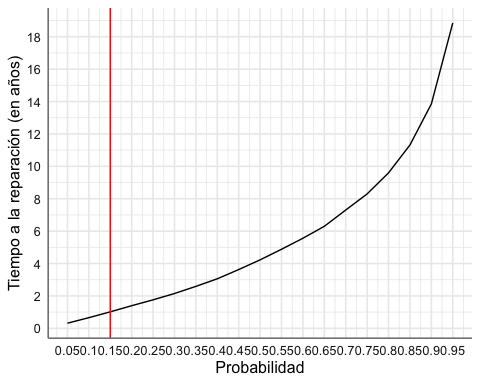
\includegraphics[width=0.95\linewidth]{01-Probabilidad_files/figure-latex/01-016-2-1} 

}

\caption{Tiempo de garantía recomendado en función de la probabilidad de que los motores necesiten reparación.}\label{fig:01-016-2}
\end{figure}

Con esta gráfica podemos establecer el tiempo de garantía en función de las especificaciones de la empresa, es decir, fijando el porcentaje de motores que necesitarán reparación.

\hypertarget{gamma}{%
\subsection{Gamma}\label{gamma}}

La distribución Gamma, al igual que ocurre con la exponencial, se utiliza habitualmente para modelizar variables aleatorias positivas y asimétricas, y sobre todo para describir procesos de eventos que ocurren en el tiempo. La función de densidad de una variable aleatoria Gamma se caracteriza por dos parámetros: \(\alpha\) o parámetro de forma, y \(\beta\) o parámetro de escala. El parámetro de forma se denomina así porque al variar su valor se obtienen diferentes formas para la fdp. La variación del parámetro de escala no cambia la forma de la distribución, pero tiende a ``estirar'' o ``comprimir'' el rango de valores sobre el que se define la probabilidad.

\begin{yellowbox}

\begin{definition}
\protect\hypertarget{def:vgamma}{}\label{def:vgamma}Una variable aleatoria \(X\), con \(x \geq 0\), tiene una distribución Gamma de parámetros \(\alpha > 0\) y \(\beta > 0\), denotada por

\[X \sim Ga(\alpha, \beta)\]

si su función de densidad viene dada por la expresión

\begin{equation}
f(x) = \frac{x^{\alpha -1} e^{-x/\beta}}{\beta^{\alpha} \Gamma(\alpha)}; \quad \text{ para } x \geq 0,
\label{eq:dgamma}
\end{equation}

con \(\Gamma()\) la función gamma, de forma que \(E(X) = \alpha\beta\) y \(V(X) = \alpha\beta^2.\)
\end{definition}

\end{yellowbox}

Un caso especial de la distribución Gamma es la \textbf{distribución Erlang}, que se denota por \(X \sim Erlang(k, \beta)\), y que se utiliza habitualmente en la modelización de sistemas de colas de espera. Su función de densidad viene dada por :

\begin{equation}
f(x) = \frac{k(kx)^{\alpha -1} e^{-xk/\beta}}{\beta^{k} (k-1)!}; \quad \text{ para } x \geq 0,
\label{eq:derlang}
\end{equation}

con \(E(x) = \beta\) y \(V(X) = \beta^2/k\). La utilidad de una variable aleatoria Erlang con parámetros \(k\) y \(\beta\) es que es el resultado de sumar \(k\) variables aleatorias exponenciales (independientes) cada una con media \(\beta/k\). En la modelización de los tiempos relacionados con un proceso industrial, la distribución exponencial suele ser inadecuada porque la desviación estándar no es tan grande como la media. Los ingenieros suelen tratar de diseñar sistemas que produzcan una desviación estándar de los tiempos del proceso que resulte significativamente menor que su media. La distribución Erlang tiene esta propiedad: su desviación estándar disminuye a medida que aumenta \(k\), de modo que los tiempos de proceso con una desviación estándar pequeña a menudo suelen ser aproximados por una variable aleatoria Erlang.

\begin{whitebox}

\begin{itemize}
\tightlist
\item
  La función \texttt{dgamma(x,\ shape,\ scale)} nos permite evaluar la función de densidad para una variable Gamma.
\item
  \texttt{pgamma(x,\ shape,\ scale)} calcula la función de distribución.
\item
  \texttt{rgamma(n,\ shape,\ scale)} permite generar \(n\) valores de una variable Gamma.
\end{itemize}

Para simular un dato de una distribución \(y \sim (Erlang(k, \beta)\)) generamos \(k\) datos exponenciales de \(x_i \sim Exp(\beta/k), i=1,\ldots,k,\) y calculamos la suma de todos esos valores,\(y=\sum_i x_i\). Repetir este proceso tantas veces como indique el tamaño de la muestra simulada que deseamos para la distribución Erlang.

\end{whitebox}

Si disponemos de la media y varianza de los datos resulta muy fácil ajustar los parámetros de la distribución Gamma o Erlang sin más que resolver las ecuaciones que nos dan el valor esperado y la varianza. Si \(\bar{x}\) y \(s^2\) son respectivamente la media y varianza, podemos ajustar los parámetros de la Gamma con:

\[ \beta = s^2/\bar{x}; \quad \alpha = \bar{x}/\beta\]

mientras que para la Erlang tenemos:

\[ \beta = \bar{x}; \quad k = \bar{x}^2/s^2.\]

A continuación se presenta la función para generar datos Erlang a patir de datos exponenciales:

\begin{Shaded}
\begin{Highlighting}[]
\CommentTok{\# Función para generar "nsim" simulaciones de una Erlang }
\CommentTok{\# con parámetros k (entero) y beta\textgreater{}0}
\NormalTok{rerlang }\OtherTok{\textless{}{-}} \ControlFlowTok{function}\NormalTok{(nsim, k, beta)}
\NormalTok{\{}
  \CommentTok{\# verificamos que k es entero}
  \ControlFlowTok{if}\NormalTok{(k}\SpecialCharTok{\%\%}\DecValTok{1} \SpecialCharTok{==} \DecValTok{0}\NormalTok{)}
\NormalTok{  \{}
    \CommentTok{\# parámetro de la exponencial}
\NormalTok{    lambda }\OtherTok{\textless{}{-}}\NormalTok{ beta}\SpecialCharTok{/}\NormalTok{k}
    \CommentTok{\# Generamos y almacenamos datos exponenciales}
\NormalTok{    datosexp }\OtherTok{\textless{}{-}} \FunctionTok{matrix}\NormalTok{(}\FunctionTok{rexp}\NormalTok{(nsim}\SpecialCharTok{*}\NormalTok{k, lambda), }\AttributeTok{nrow =}\NormalTok{ nsim)}
    \CommentTok{\# Obtenemos la muestra de la Erlang}
\NormalTok{    datoserl }\OtherTok{\textless{}{-}} \FunctionTok{apply}\NormalTok{(datosexp, }\DecValTok{1}\NormalTok{, sum)}
    \FunctionTok{return}\NormalTok{(datoserl)}
\NormalTok{  \}}
  \ControlFlowTok{else}\NormalTok{\{}
    \FunctionTok{cat}\NormalTok{(}\StringTok{"k debe ser entero"}\NormalTok{)}
\NormalTok{  \}}
\NormalTok{\}}
\end{Highlighting}
\end{Shaded}

\hypertarget{weibull}{%
\subsection{Weibull}\label{weibull}}

La distribución Weibull se utiliza para describir la resistencia a la rotura de diversos materiales o para describir los tiempos de fallo de muchos tipos de sistemas diferentes. La distribución Weibull tiene dos parámetros: un parámetro de escala, \(\beta\) , y un parámetro de forma \(\alpha\), ambos positivos. La funcion de distribución asociada viene dada por:

\begin{equation}
F(x) = 
\begin{cases}
0 & \text{ si } x < 0 \\
1 - e^{-(x/\beta)^{\alpha}} & \text{ si } x \geq 0
\end{cases}
\label{eq:var-weibull2}
\end{equation}

Como en el caso de la distribución Gamma el parámetro de forma determina la forma general de la fdp y el parámetro de escala expande o contrae la fdp.

\begin{yellowbox}

\begin{definition}
\protect\hypertarget{def:vweibull}{}\label{def:vweibull}Una variable aleatoria \(X\) tiene una distribución Weibull de parámetros \(\alpha>0\) y \(\beta>0\), que se denota por

\[X \sim Weib(\alpha, \beta)\]

si su función de densidad viene dada por la expresión

\begin{equation}
f(x)=\frac{\alpha}{\beta}\frac{x}{\beta}^{\alpha-1}e^{-(x/\beta)^{\alpha}}, \quad x \geq 0.
\label{eq:var-weibull}
\end{equation}

El valor esperado y la varianza vienen dados por:

\[E(X) = \beta \Gamma(1 + 1/\alpha); \quad V(X) = \beta^2 (\Gamma(1 + 2/\alpha) - (\Gamma(1 + 1/\alpha))^2).\]
\end{definition}

\end{yellowbox}

En \texttt{R} tenemos las siguientes funciones relacionadas con la distribución Weibull.

\begin{whitebox}

\begin{itemize}
\tightlist
\item
  La función \texttt{dweibull(x,\ shape,\ scale)} nos permite evaluar la función de densidad para una variable Weibull
\item
  \texttt{pweibull(x,\ shape,\ scale)} calcula la función de distribución.
\item
  \texttt{rweibull(n,\ shape,\ scale)} permite generar \(n\) valores de una variable Weibull.
\end{itemize}

\end{whitebox}

A partir de la media (\(\bar{x}\)) y varianza (\(S^2\)) de un conjunto de datos, es posible obtener los parámetros de la distribución Weibull sin más que resolver las ecuaciones:

\begin{eqnarray}
\beta &=& \frac{\bar{x}}{\Gamma(1 + 1/ \alpha)} \\
\frac{s^2}{\bar{x}^2} - \frac{\Gamma(1+ 2/\alpha)}{(\Gamma(1 + 1/ \alpha))^2} + 1 &=& 0.
\label{eq:estimaweibuleq}
\end{eqnarray}

A continuación se propone una función que permite obtener los parámetros a partir de la media y varianza de los datos, junto con un pequeño ejemplo para verificar su funcionalidad.

\begin{Shaded}
\begin{Highlighting}[]
\NormalTok{estima.weibull }\OtherTok{\textless{}{-}} \ControlFlowTok{function}\NormalTok{(m, s)}
\NormalTok{\{}
  \CommentTok{\#m=media, s=desviación típica}
  \FunctionTok{library}\NormalTok{(rootSolve)}
  \CommentTok{\# Función para optimizar alpha}
\NormalTok{  fun.alpha }\OtherTok{\textless{}{-}} \ControlFlowTok{function}\NormalTok{(a, m, s)}
\NormalTok{              \{}
\NormalTok{                res}\OtherTok{\textless{}{-}} \DecValTok{1} \SpecialCharTok{+}\NormalTok{ (s}\SpecialCharTok{/}\NormalTok{m)}\SpecialCharTok{\^{}}\DecValTok{2} \SpecialCharTok{{-}} \FunctionTok{gamma}\NormalTok{(}\DecValTok{1}\SpecialCharTok{+}\DecValTok{2}\SpecialCharTok{/}\NormalTok{a)}\SpecialCharTok{/}\NormalTok{(}\FunctionTok{gamma}\NormalTok{(}\DecValTok{1}\SpecialCharTok{+}\DecValTok{1}\SpecialCharTok{/}\NormalTok{a))}\SpecialCharTok{\^{}}\DecValTok{2}
                \FunctionTok{return}\NormalTok{(res)}
\NormalTok{              \}}
  \CommentTok{\# Obtención de alpha}
\NormalTok{    alpha }\OtherTok{\textless{}{-}} \FunctionTok{round}\NormalTok{(}\FunctionTok{uniroot}\NormalTok{(fun.alpha, }\FunctionTok{c}\NormalTok{(}\FloatTok{0.1}\NormalTok{, }\DecValTok{10000}\NormalTok{),}\AttributeTok{m=}\NormalTok{m,}\AttributeTok{s=}\NormalTok{s)}\SpecialCharTok{$}\NormalTok{root,}\DecValTok{2}\NormalTok{)}
  \CommentTok{\# Obtención de beta}
\NormalTok{  beta }\OtherTok{\textless{}{-}} \FunctionTok{round}\NormalTok{(m}\SpecialCharTok{/}\FunctionTok{gamma}\NormalTok{(}\DecValTok{1}\SpecialCharTok{+}\DecValTok{1}\SpecialCharTok{/}\NormalTok{alpha), }\DecValTok{2}\NormalTok{)}
  \CommentTok{\# Devolvemos alpha y beta}
  \FunctionTok{return}\NormalTok{(}\FunctionTok{c}\NormalTok{(alpha, beta))}
\NormalTok{\}}

\CommentTok{\# Datos de ejemplo}
\NormalTok{m }\OtherTok{\textless{}{-}} \DecValTok{80}     \CommentTok{\# media}
\NormalTok{s }\OtherTok{\textless{}{-}} \FunctionTok{sqrt}\NormalTok{(}\DecValTok{50}\NormalTok{)  }\CommentTok{\# desviación típica}
\CommentTok{\# Estimación}
\NormalTok{res}\OtherTok{=}\FunctionTok{estima.weibull}\NormalTok{(m,s)}
\FunctionTok{cat}\NormalTok{(}\StringTok{"Weibull alpha="}\NormalTok{,res[}\DecValTok{1}\NormalTok{],}\StringTok{", Weibull beta="}\NormalTok{,res[}\DecValTok{2}\NormalTok{])}
\end{Highlighting}
\end{Shaded}

\begin{verbatim}
## Weibull alpha= 13.83 , Weibull beta= 83.06
\end{verbatim}

\hypertarget{normal}{%
\subsection{Normal}\label{normal}}

La distribución normal es la distribución más común, reconocida por la mayoría de personas por su curva en forma de ``campana'', y también llamada ``campana de Gauss''. Aunque la distribución normal no se utiliza mucho en la modelización de procesos y sitemas, es sin duda, la más relevante de las distribuciones aleatorias, ya que representa el supuesto básico distribucional para resolver muchos de los problemas de inferencia estadística habituales, como veremos en la sección final de esta unidad.

\begin{yellowbox}

\begin{definition}
\protect\hypertarget{def:vnormal}{}\label{def:vnormal}Una variable aleatoria \(X\) tiene una distribución Normal de parámetros \(\mu\) y \(\sigma\) con \(\sigma >0\), denotada por

\[ X \sim N(\mu, \sigma^2),\]

si su función de densidad viene dada por

\begin{equation}
f(x) = \frac{1}{\sigma\sqrt{2\pi}} exp\left(\frac{-(x-\mu)^2}{2\sigma^2}\right), \quad x \in R
\end{equation}

con \(E(X) = \mu\) y \(V(X) = \sigma^2\), y que se denota:
\end{definition}

\end{yellowbox}

El parámetro \(\mu\) identifica la media, y por lo tanto el centro de la distribución al ser simétrica, y el parámetro \(\sigma\) la desviación típica.

El caso más destacado es la denominada distribución \textbf{Normal estándar}, para la que \(\mu = 0\) y \(\sigma = 1\), por su utilización en problemas inferenciales sencillos donde la variabilidad es conocida.

A partir de cualquier distribución Normal podemos transformar a una distribución Normal estándar. Si \(X \sim N(\mu, \sigma^2)\) entonces la variable aleatoria \(Z\) definida como

\[Z = \frac{X - \mu}{\sigma} \sim N(0,1).\]

Vinculadas a la distribución Normal surgen las distribuciones \(t\) de Student, \textbf{Chi-chadrado} y \(F\) de Snedecor (también llamada de Fisher-Snedecor), que son ampliamente utilizadas en inferencia estadística. En el último apartado de esta unidad veremos cómo utilizar estas distrbuciones para resolver mediante simulación problemas de intervalos de confianza o contrastes de hipótesis.

Si \(\bar{X_n}=\sum_i X_i/n\) representa la media muestral de \(n\) v.a. \(N(\mu,\sigma)\) y \(S^2=\sum_i(X_i-\bar{X_n})^2/(n-1)\) su varianza muestral, entonces la variable \(Y\) \[ Y= \frac{\bar{X_n}-\mu}{S/\sqrt{n}}\sim St(n-1)\] sigue una distribución t de Student con \(n-1\) grados de libertad, y se denota por \(Y\sim St(n-1)\).

Si tenemos un conjunto de variables normales estándar independientes, \(X_i\sim N(0,1), i=1,\ldots,n\), entonces su suma al cuadrado sigue una distribución chi-cuadrado con \(n\) grados de libertad. \[Z=\sum_{i=1}^n X_i^2 \sim \chi^2_{n}\] Por último, a partir de dos distribuciones chi-cuadrado independientes, \(U\sim \chi^2_n\) y \(V\sim \chi^2_m\), tenemos que su cociente, corregido por sus grados de libertad, sigue una distribución F de Snedecor con \(n\) y \(m\) grados de libertad, \[ W=\frac{U/n}{V/m} \sim F_{(n,m)}.\]

\begin{whitebox}
Para la distribución Normal,

\begin{itemize}
\tightlist
\item
  La función \texttt{dnorm(x,\ mean,\ sd)} nos permite evaluar la función de densidad para una variable Normal.
\item
  \texttt{pnorm(x,\ mean,\ sd)} calcula la función de distribución.
\item
  \texttt{rnorm(n,\ mean,\ sd)} permite generar \(n\) valores de una variable Normal.
\end{itemize}

Para la distribución t de Student con \(df1\) grados de libertad, las funciones correspondientes son \texttt{dt(x,\ df1)}, \texttt{pt(x,\ df1)} y \texttt{rt(n,df1)}.

Para la distribución chi-cuadrado con \(df1\) grados de libertad, contamos con las funciones \texttt{dchisq(x,df1)}, \texttt{pchisq(x,df1)} y \texttt{rchisq(n,df1)} respectivamente.

Para la distribución F de Snedecor con \(df1\) y \(df2\) grados de libertad, tenemos las correspondencias \texttt{df(x,\ df1,\ df2)}, \texttt{pf(x,\ df1,\ df2)} y \texttt{rf(n,df1,df2)}.

\end{whitebox}

En la Figura \ref{fig:graficosnormal} aparecen representadas varias distribuciones normales con distinta media y varianza.

\begin{Shaded}
\begin{Highlighting}[]
\NormalTok{x}\OtherTok{=}\FunctionTok{seq}\NormalTok{(}\SpecialCharTok{{-}}\DecValTok{10}\NormalTok{,}\DecValTok{10}\NormalTok{,}\FloatTok{0.1}\NormalTok{)}
\NormalTok{y1}\OtherTok{=}\FunctionTok{dnorm}\NormalTok{(x)}
\NormalTok{y2}\OtherTok{=}\FunctionTok{dnorm}\NormalTok{(x,}\DecValTok{0}\NormalTok{,}\DecValTok{3}\NormalTok{)}
\NormalTok{y3}\OtherTok{=}\FunctionTok{dnorm}\NormalTok{(x,}\DecValTok{2}\NormalTok{,}\DecValTok{1}\NormalTok{)}
\NormalTok{y4}\OtherTok{=}\FunctionTok{dnorm}\NormalTok{(x,}\DecValTok{2}\NormalTok{,}\DecValTok{3}\NormalTok{)}
\NormalTok{datos}\OtherTok{=}\FunctionTok{as.tibble}\NormalTok{(}\FunctionTok{cbind}\NormalTok{(x,y1,y2,y3,y4))}
\end{Highlighting}
\end{Shaded}

\begin{verbatim}
## Warning: `as.tibble()` was deprecated in tibble 2.0.0.
## Please use `as_tibble()` instead.
## The signature and semantics have changed, see `?as_tibble`.
## This warning is displayed once every 8 hours.
## Call `lifecycle::last_lifecycle_warnings()` to see where this warning was generated.
\end{verbatim}

\begin{Shaded}
\begin{Highlighting}[]
\NormalTok{levels}\OtherTok{=}\FunctionTok{c}\NormalTok{(}\StringTok{"N(0,1)"}\OtherTok{=}\StringTok{"y1"}\NormalTok{,}\StringTok{"N(0,3)"}\OtherTok{=}\StringTok{"y2"}\NormalTok{,}\StringTok{"N(2,1)"}\OtherTok{=}\StringTok{"y3"}\NormalTok{,}\StringTok{"N(2,3)"}\OtherTok{=}\StringTok{"y4"}\NormalTok{)}
\NormalTok{datos}\OtherTok{=}\NormalTok{datos }\SpecialCharTok{\%\textgreater{}\%}
  \FunctionTok{pivot\_longer}\NormalTok{(}\AttributeTok{cols=}\DecValTok{2}\SpecialCharTok{:}\DecValTok{5}\NormalTok{,}\AttributeTok{names\_to=}\StringTok{"tipo"}\NormalTok{,}\AttributeTok{values\_to=}\StringTok{"valor"}\NormalTok{) }
\NormalTok{datos}\SpecialCharTok{$}\NormalTok{tipo}\OtherTok{=}\FunctionTok{fct\_recode}\NormalTok{(datos}\SpecialCharTok{$}\NormalTok{tipo,}\SpecialCharTok{!!!}\NormalTok{levels)}

\FunctionTok{ggplot}\NormalTok{(datos,}\FunctionTok{aes}\NormalTok{(}\AttributeTok{x=}\NormalTok{x,}\AttributeTok{y=}\NormalTok{valor,}\AttributeTok{color=}\NormalTok{tipo))}\SpecialCharTok{+}
  \FunctionTok{geom\_line}\NormalTok{()}\SpecialCharTok{+}
  \FunctionTok{labs}\NormalTok{(}\AttributeTok{color=}\StringTok{"Distribuciones"}\NormalTok{,}\AttributeTok{y=}\StringTok{"Función de densidad"}\NormalTok{)}
\end{Highlighting}
\end{Shaded}

\begin{figure}

{\centering 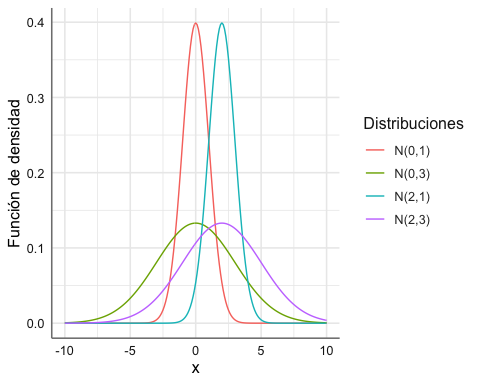
\includegraphics[width=0.95\linewidth]{01-Probabilidad_files/figure-latex/graficosnormal-1} 

}

\caption{Funciones de densidad para varias distribuciones normales.}\label{fig:graficosnormal}
\end{figure}

En la Figura \ref{fig:graficost} aparecen representadas varias distribuciones t de Student con distintos grados de libertad.

\begin{Shaded}
\begin{Highlighting}[]
\NormalTok{x}\OtherTok{=}\FunctionTok{seq}\NormalTok{(}\SpecialCharTok{{-}}\DecValTok{5}\NormalTok{,}\DecValTok{5}\NormalTok{,}\FloatTok{0.1}\NormalTok{)}
\NormalTok{y1}\OtherTok{=}\FunctionTok{dt}\NormalTok{(x,}\DecValTok{2}\NormalTok{)}
\NormalTok{y2}\OtherTok{=}\FunctionTok{dt}\NormalTok{(x,}\DecValTok{5}\NormalTok{)}
\NormalTok{y3}\OtherTok{=}\FunctionTok{dt}\NormalTok{(x,}\DecValTok{10}\NormalTok{)}
\NormalTok{y4}\OtherTok{=}\FunctionTok{dnorm}\NormalTok{(x)}
\NormalTok{datos}\OtherTok{=}\FunctionTok{as.tibble}\NormalTok{(}\FunctionTok{cbind}\NormalTok{(x,y1,y2,y3,y4))}
\NormalTok{levels}\OtherTok{=}\FunctionTok{c}\NormalTok{(}\StringTok{"St(2)"}\OtherTok{=}\StringTok{"y1"}\NormalTok{,}\StringTok{"St(5)"}\OtherTok{=}\StringTok{"y2"}\NormalTok{,}\StringTok{"St(10)"}\OtherTok{=}\StringTok{"y3"}\NormalTok{,}\StringTok{"N(0,1)"}\OtherTok{=}\StringTok{"y4"}\NormalTok{)}
\NormalTok{datos}\OtherTok{=}\NormalTok{datos }\SpecialCharTok{\%\textgreater{}\%}
  \FunctionTok{pivot\_longer}\NormalTok{(}\AttributeTok{cols=}\DecValTok{2}\SpecialCharTok{:}\DecValTok{5}\NormalTok{,}\AttributeTok{names\_to=}\StringTok{"tipo"}\NormalTok{,}\AttributeTok{values\_to=}\StringTok{"valor"}\NormalTok{) }
\NormalTok{datos}\SpecialCharTok{$}\NormalTok{tipo}\OtherTok{=}\FunctionTok{fct\_recode}\NormalTok{(datos}\SpecialCharTok{$}\NormalTok{tipo,}\SpecialCharTok{!!!}\NormalTok{levels)}

\FunctionTok{ggplot}\NormalTok{(datos,}\FunctionTok{aes}\NormalTok{(}\AttributeTok{x=}\NormalTok{x,}\AttributeTok{y=}\NormalTok{valor,}\AttributeTok{color=}\NormalTok{tipo))}\SpecialCharTok{+}
  \FunctionTok{geom\_line}\NormalTok{()}\SpecialCharTok{+}
  \FunctionTok{labs}\NormalTok{(}\AttributeTok{color=}\StringTok{"Distribuciones"}\NormalTok{,}\AttributeTok{y=}\StringTok{"Función de densidad"}\NormalTok{)}
\end{Highlighting}
\end{Shaded}

\begin{figure}

{\centering 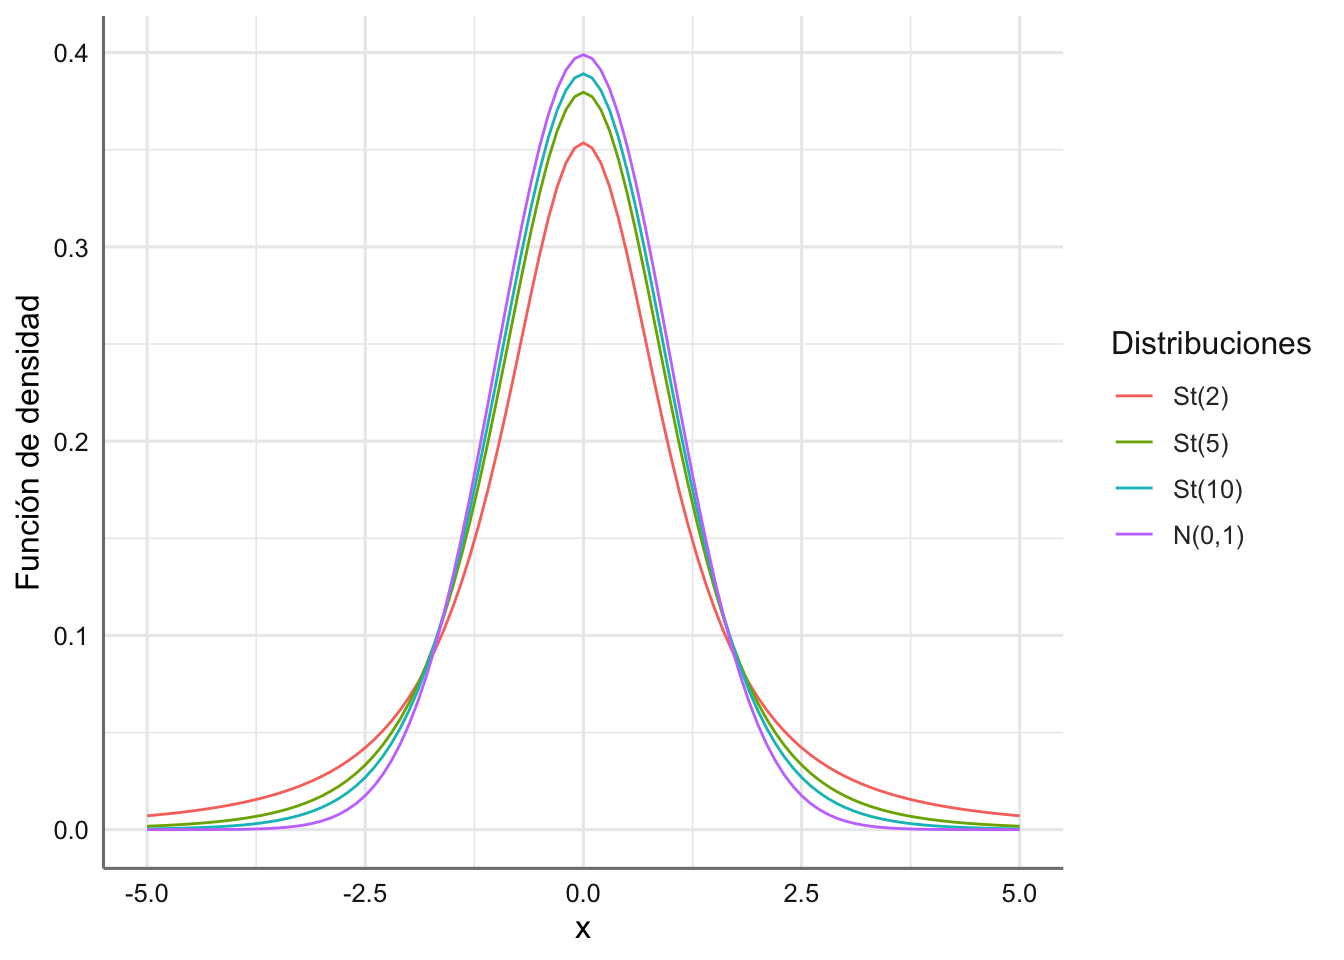
\includegraphics[width=0.95\linewidth]{01-Probabilidad_files/figure-latex/graficost-1} 

}

\caption{Funciones de densidad para varias distribuciones T de Student.}\label{fig:graficost}
\end{figure}

En la Figura \ref{fig:graficoschi2} aparecen representadas varias distribuciones chi-cuadrado con distintos grados de libertad.

\begin{Shaded}
\begin{Highlighting}[]
\NormalTok{x}\OtherTok{=}\FunctionTok{seq}\NormalTok{(}\DecValTok{0}\NormalTok{,}\DecValTok{200}\NormalTok{,}\FloatTok{0.1}\NormalTok{)}
\NormalTok{y1}\OtherTok{=}\FunctionTok{dchisq}\NormalTok{(x,}\DecValTok{5}\NormalTok{)}
\NormalTok{y2}\OtherTok{=}\FunctionTok{dchisq}\NormalTok{(x,}\DecValTok{10}\NormalTok{)}
\NormalTok{y3}\OtherTok{=}\FunctionTok{dchisq}\NormalTok{(x,}\DecValTok{50}\NormalTok{)}
\NormalTok{y4}\OtherTok{=}\FunctionTok{dchisq}\NormalTok{(x,}\DecValTok{100}\NormalTok{)}
\NormalTok{datos}\OtherTok{=}\FunctionTok{as.tibble}\NormalTok{(}\FunctionTok{cbind}\NormalTok{(x,y1,y2,y3,y4))}
\NormalTok{levels}\OtherTok{=}\FunctionTok{c}\NormalTok{(}\StringTok{"Chi2(5)"}\OtherTok{=}\StringTok{"y1"}\NormalTok{,}\StringTok{"Chi2(10)"}\OtherTok{=}\StringTok{"y2"}\NormalTok{,}\StringTok{"Chi2(50)"}\OtherTok{=}\StringTok{"y3"}\NormalTok{,}\StringTok{"Chi2(100)"}\OtherTok{=}\StringTok{"y4"}\NormalTok{)}
\NormalTok{datos}\OtherTok{=}\NormalTok{datos }\SpecialCharTok{\%\textgreater{}\%}
  \FunctionTok{pivot\_longer}\NormalTok{(}\AttributeTok{cols=}\DecValTok{2}\SpecialCharTok{:}\DecValTok{5}\NormalTok{,}\AttributeTok{names\_to=}\StringTok{"tipo"}\NormalTok{,}\AttributeTok{values\_to=}\StringTok{"valor"}\NormalTok{) }
\NormalTok{datos}\SpecialCharTok{$}\NormalTok{tipo}\OtherTok{=}\FunctionTok{fct\_recode}\NormalTok{(datos}\SpecialCharTok{$}\NormalTok{tipo,}\SpecialCharTok{!!!}\NormalTok{levels)}

\FunctionTok{ggplot}\NormalTok{(datos,}\FunctionTok{aes}\NormalTok{(}\AttributeTok{x=}\NormalTok{x,}\AttributeTok{y=}\NormalTok{valor,}\AttributeTok{color=}\NormalTok{tipo))}\SpecialCharTok{+}
  \FunctionTok{geom\_line}\NormalTok{()}\SpecialCharTok{+}
  \FunctionTok{labs}\NormalTok{(}\AttributeTok{color=}\StringTok{"Distribuciones"}\NormalTok{,}\AttributeTok{y=}\StringTok{"Función de densidad"}\NormalTok{)}
\end{Highlighting}
\end{Shaded}

\begin{figure}

{\centering 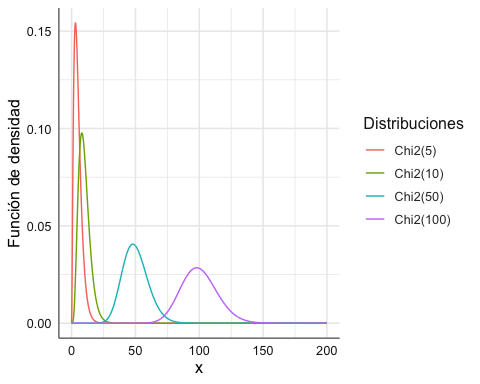
\includegraphics[width=0.95\linewidth]{01-Probabilidad_files/figure-latex/graficoschi2-1} 

}

\caption{Funciones de densidad para varias distribuciones Chi-cuadrado.}\label{fig:graficoschi2}
\end{figure}

En la Figura \ref{fig:graficosf} aparecen representadas varias distribuciones F de Snedecor con distintos grados de libertad.

\begin{Shaded}
\begin{Highlighting}[]
\NormalTok{x}\OtherTok{=}\FunctionTok{seq}\NormalTok{(}\DecValTok{0}\NormalTok{,}\DecValTok{5}\NormalTok{,}\FloatTok{0.01}\NormalTok{)}
\NormalTok{y1}\OtherTok{=}\FunctionTok{df}\NormalTok{(x,}\DecValTok{5}\NormalTok{,}\DecValTok{5}\NormalTok{)}
\NormalTok{y2}\OtherTok{=}\FunctionTok{df}\NormalTok{(x,}\DecValTok{1}\NormalTok{,}\DecValTok{5}\NormalTok{)}
\NormalTok{y3}\OtherTok{=}\FunctionTok{df}\NormalTok{(x,}\DecValTok{50}\NormalTok{,}\DecValTok{10}\NormalTok{)}
\NormalTok{y4}\OtherTok{=}\FunctionTok{df}\NormalTok{(x,}\DecValTok{100}\NormalTok{,}\DecValTok{200}\NormalTok{)}
\NormalTok{datos}\OtherTok{=}\FunctionTok{as.tibble}\NormalTok{(}\FunctionTok{cbind}\NormalTok{(x,y1,y2,y3,y4))}
\NormalTok{levels}\OtherTok{=}\FunctionTok{c}\NormalTok{(}\StringTok{"F(5,5)"}\OtherTok{=}\StringTok{"y1"}\NormalTok{,}\StringTok{"F(1,5)"}\OtherTok{=}\StringTok{"y2"}\NormalTok{,}\StringTok{"F(50,10)"}\OtherTok{=}\StringTok{"y3"}\NormalTok{,}\StringTok{"F(100,200)"}\OtherTok{=}\StringTok{"y4"}\NormalTok{)}
\NormalTok{datos}\OtherTok{=}\NormalTok{datos }\SpecialCharTok{\%\textgreater{}\%}
  \FunctionTok{pivot\_longer}\NormalTok{(}\AttributeTok{cols=}\DecValTok{2}\SpecialCharTok{:}\DecValTok{5}\NormalTok{,}\AttributeTok{names\_to=}\StringTok{"tipo"}\NormalTok{,}\AttributeTok{values\_to=}\StringTok{"valor"}\NormalTok{) }
\NormalTok{datos}\SpecialCharTok{$}\NormalTok{tipo}\OtherTok{=}\FunctionTok{fct\_recode}\NormalTok{(datos}\SpecialCharTok{$}\NormalTok{tipo,}\SpecialCharTok{!!!}\NormalTok{levels)}

\FunctionTok{ggplot}\NormalTok{(datos,}\FunctionTok{aes}\NormalTok{(}\AttributeTok{x=}\NormalTok{x,}\AttributeTok{y=}\NormalTok{valor,}\AttributeTok{color=}\NormalTok{tipo))}\SpecialCharTok{+}
  \FunctionTok{geom\_line}\NormalTok{()}\SpecialCharTok{+}
  \FunctionTok{labs}\NormalTok{(}\AttributeTok{color=}\StringTok{"Distribuciones"}\NormalTok{,}\AttributeTok{y=}\StringTok{"Función de densidad"}\NormalTok{)}
\end{Highlighting}
\end{Shaded}

\begin{figure}

{\centering 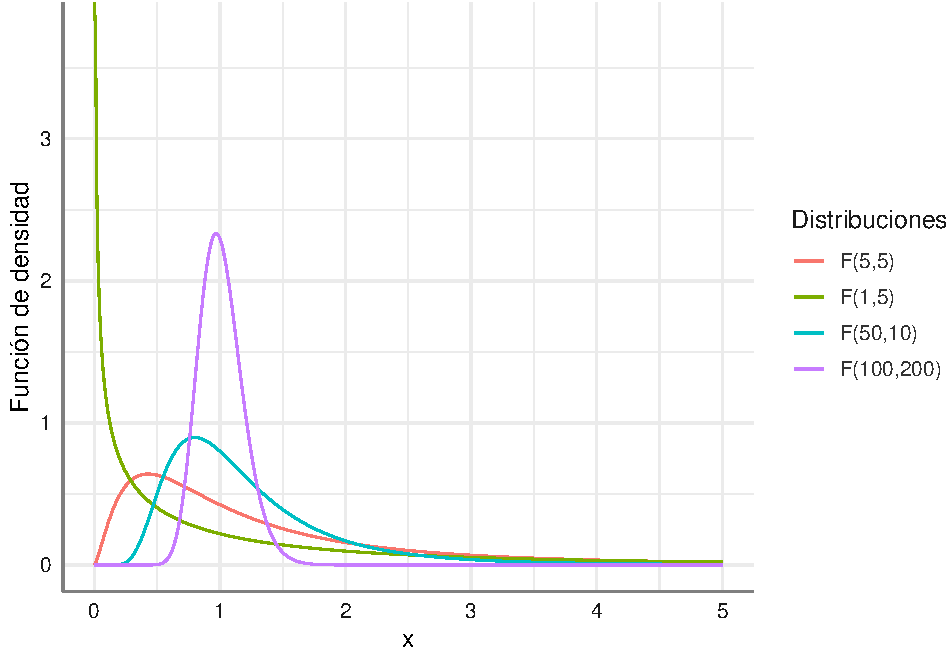
\includegraphics[width=0.95\linewidth]{01-Probabilidad_files/figure-latex/graficosf-1} 

}

\caption{Funciones de densidad para varias distribuciones F-Snedecor.}\label{fig:graficosf}
\end{figure}

\hypertarget{transformadainversa}{%
\section{Simular con la Transformada Inversa}\label{transformadainversa}}

Aunque las distribuciones estudiadas en el punto anterior, al ser habituales provocan que los algoritmos de simulación y sus funciones de probabilidad ya estén implementadas en la mayoría de los paquetes estadísticos y de cálculo, en otras ocasiones, ante otras distribuciones menos comunes, no disponemos de un método directo para la simulación de muestras aleatorias, y necesitamos recurrir a algoritmos genéricos de simulación de variables.

Presentamos a continuación un algoritmo genérico para simular de variables discretas o continuas definidas a trozos: el \textbf{algoritmo de la transformada inversa}, que pasamos a describir, tanto para variables continuas como para variables discretas.

\begin{yellowbox}

\begin{definition}
\protect\hypertarget{def:aticontinua}{}\label{def:aticontinua}\textbf{Algoritmo de la transformada inversa para variables continuas}

Dada una variable aleatoria \(X\) de tipo continuo, cuya función de distribución viene dada por \(F(x)\), y cuya función de distribución inversa se denota por \(F^{-1}(x)\), el algoritmo de la transformada inversa permite obtener una muestra de tamaño \(n\) de la variable \(X\) mediante el siguiente procedimiento:

\begin{itemize}
\tightlist
\item
  Generar \(n\) valores uniformes en el intervalo \([0,1]\),
\end{itemize}

\[u_i\sim U(0,1), \quad i=1,...,n\]

\begin{itemize}
\tightlist
\item
  Devolver \(x_i = F^{-1}(u_i)\).
\end{itemize}

Así los valores \(\{x_1,...,x_n\}\) constituyen una muestra de \(X\).
\end{definition}

\end{yellowbox}

El algoritmo es conceptualmente similar para variables discretas, si bien por la discretización, varía levemente.

\begin{yellowbox}

\begin{definition}
\protect\hypertarget{def:atidiscreta}{}\label{def:atidiscreta}\textbf{Algoritmo de la transformada inversa para variables discretas}

Dada una variable aleatoria \(X\), de tipo discreto, con \(k\) posibles valores diferentes \(x_1,...,x_k\), y cuya función de distribución viene dada por:

\[F(x) = Pr(X \leq x) = \sum_{x_i \leq x} Pr(X = x_i), i=1,...,k,\]

el algoritmo de la transformada inversa permite obtener una muestra de tamaño \(n\) de la variable \(X\) mediante el siguiente procedimiento:

\begin{itemize}
\tightlist
\item
  Generar \(n\) valores uniformes en el intervalo \([0,1]\), \[u_i\sim U(0,1), \quad i=1,...,n\]
\item
  Para cada \(u_i\) generado se determina el entero \(I\) más pequeño que satisface \(u_i \leq F(x_I)\), del conjunto \(\{x_1,...,x_k\}\)
\item
  Devolver \(x_I\) para cada valor simulado.
\end{itemize}

Así los valores \(\{x_1,...,x_n\}\) constituyen una muestra de \(X\).
\end{definition}

\end{yellowbox}

En los puntos siguientes vamos a mostrar el uso de los algoritmos \ref{def:aticontinua} y \ref{def:atidiscreta} en diferentes ejemplos de variables de tipo discreto y continuo.

\hypertarget{otras-distribuciones-discretas}{%
\section{Otras distribuciones discretas}\label{otras-distribuciones-discretas}}

Analizamos diferentes ejemplos en los que estamos interesados en evaluar un sistema que involucra a una o más variables de tipo discreto, y donde únicamente disponemos de información sobre la función de masa de probabilidad o sobre la función de distribución.

\hypertarget{una-variable-discreta}{%
\subsection{Una variable discreta}\label{una-variable-discreta}}

Supongamos un sistema en el que contamos con información de una única variable discreta de interés que deseamos estudiar. En los casos más sencillos que tratamos aquí, las situaciones planteadas se pueden resolver teóricamente sin mucha dificultad, pero el objetivo es mostrar el uso de la simulación para llegar a resultados aproximados a los que proporcionan los métodos análiticos.

\begin{example}
\protect\hypertarget{exm:discreta1}{}\label{exm:discreta1}Una empresa que fabrica piezas para maquinaria de fabricación de calzado tiene diseñada la cadena de producción de tal forma que las piezas fabricadas se almacenan (y venden) en cajas de dos unidades. El beneficio estimado de una caja sin defectos es de 300 euros. La política de la empresa establece que si al servir una caja a los clientes, esta contiene una pieza defectuosa, debe ser devuelta de forma inmediata para su reemplazo, lo que supone una pérdida de 50 euros por pieza defectuosa (y la devolución de los 300 euros de beneficio por la venta). El problema es que una vez cerradas las cajas en la cadena de producción no se inspeccionan para estimar el número de cajas que se podrían devolver. La única información disponible hace referencia a la tasa de defectos observada en cada caja cuando esta es devuelta, junto con el porcentaje de cajas que son devueltas. En base a esta información, si \(N\) refleja el número de piezas defectuosas observadas, la empresa ha establecido que:

\begin{equation}
Pr(N = k) = 
\begin{cases}
0.82 & \text{ para } k = 0\\
0.15 & \text{ para } k = 1\\
0.03 & \text{ para } k = 2\\
\end{cases}
\label{eq:var-discreta1}
\end{equation}

La empresa quiere estudiar el beneficio estimado de acuerdo a la politica de producción actual para el próximo mes, sabiendo que se pueden llegar a producir hasta 1500 cajas en ese periodo. Además la empresa está interesada en conocer el beneficio estimado si cambiara su politica de calidad reduciendo su tasa de defectos por caja de acuerdo a las siguientes proporciones:

\begin{equation}
Pr(N = k) = 
\begin{cases}
0.85 & \text{ para } k = 0\\
0.13 & \text{ para } k = 1\\
0.02 & \text{ para } k = 2\\
\end{cases}
\label{eq:var-discreta1-1}
\end{equation}
\end{example}

Para resolver las inquietudes de la empresa, vamos a simular el proceso en las dos situaciones planteadas, para el horizonte propuesto de un mes, esto es, simulando las 1500 cajas y estimando el beneficio obtenido de acuerdo a las políticas de calidad dadas en \eqref{eq:var-discreta1} y \eqref{eq:var-discreta1-1}.

Proponemos el siguiente algoritmo de simulación para obtener la ganancia asociada a cada una de las políticas de calidad, y con dichas ganancias compararlas y concluir cuál es la más beneficiosa.

\begin{silverbox}
\textbf{Algoritmo de simulación} Ante una política de calidad:

\begin{enumerate}
\def\labelenumi{\arabic{enumi}.}
\tightlist
\item
  Fijar las condiciones de simulación: nº cajas (\(nsim = 1500\)).
\item
  Obtener las función de distribución acumulada vinculada con la politica de calidad de interés y aplicar el algoritmo dado en al definición \ref{def:atidiscreta} para obtener una muestra de \(N\), \(x_1,...,x_n\), relativas al número de piezas defectuosas en cada caja.
\item
  Calcular el beneficio obtenido para cada caja, vinculado a cada valor \(x_i\), denominado \(b_i\).
\item
  Obtener la ganancia global con todas las cajas simuladas como:
\end{enumerate}

\[G = \sum_{i=1}^n b_i\]

\end{silverbox}

Lancemos el algoritmo para cada situación y obtengamos los beneficios esperados.

\begin{Shaded}
\begin{Highlighting}[]
\CommentTok{\# Parámetros de la simulación}
\FunctionTok{set.seed}\NormalTok{(}\DecValTok{19}\NormalTok{)}
\NormalTok{nsim }\OtherTok{\textless{}{-}} \DecValTok{1500}
\CommentTok{\# datos uniformes}
\NormalTok{unif }\OtherTok{\textless{}{-}} \FunctionTok{runif}\NormalTok{(nsim)}
\CommentTok{\# Valores a devolver (piezas defectuosas por caja)}
\NormalTok{valores }\OtherTok{\textless{}{-}} \FunctionTok{c}\NormalTok{(}\DecValTok{0}\NormalTok{, }\DecValTok{1}\NormalTok{, }\DecValTok{2}\NormalTok{)}
\CommentTok{\# Valores a devolver y probabilidad acumulada para la política 1}
\NormalTok{prob1 }\OtherTok{\textless{}{-}} \FunctionTok{c}\NormalTok{(}\FloatTok{0.82}\NormalTok{, }\FloatTok{0.15}\NormalTok{, }\FloatTok{0.03}\NormalTok{)}
\NormalTok{probacum1 }\OtherTok{\textless{}{-}} \FunctionTok{cumsum}\NormalTok{(prob1)}
\CommentTok{\# Valores a devolver y probabilidad acumulada para la política 2}
\NormalTok{prob2 }\OtherTok{\textless{}{-}} \FunctionTok{c}\NormalTok{(}\FloatTok{0.85}\NormalTok{, }\FloatTok{0.13}\NormalTok{, }\FloatTok{0.02}\NormalTok{)}
\NormalTok{probacum2 }\OtherTok{\textless{}{-}} \FunctionTok{cumsum}\NormalTok{(prob2)}
\CommentTok{\# Inicialización de variables donde almacenamos las simulaciones}
\NormalTok{xs1 }\OtherTok{\textless{}{-}} \FunctionTok{c}\NormalTok{(); benef1 }\OtherTok{\textless{}{-}} \FunctionTok{c}\NormalTok{()}
\NormalTok{xs2 }\OtherTok{\textless{}{-}} \FunctionTok{c}\NormalTok{(); benef2 }\OtherTok{\textless{}{-}} \FunctionTok{c}\NormalTok{()}
\CommentTok{\# Simulación de la variable de interés}
\NormalTok{i }\OtherTok{\textless{}{-}} \DecValTok{1}
\ControlFlowTok{while}\NormalTok{ (i }\SpecialCharTok{\textless{}=}\NormalTok{ nsim)}
\NormalTok{\{}
  \CommentTok{\# politica 1}
\NormalTok{  xs1[i] }\OtherTok{\textless{}{-}}\NormalTok{ valores[}\FunctionTok{min}\NormalTok{(}\FunctionTok{which}\NormalTok{(unif[i] }\SpecialCharTok{\textless{}=}\NormalTok{ probacum1))] }
\NormalTok{  benef1[i] }\OtherTok{\textless{}{-}} \FunctionTok{ifelse}\NormalTok{(xs1[i]}\SpecialCharTok{==}\DecValTok{0}\NormalTok{, }\DecValTok{300}\NormalTok{, }\SpecialCharTok{{-}}\DecValTok{50}\SpecialCharTok{*}\NormalTok{xs1[i]) }\CommentTok{\# beneficios}
  \CommentTok{\# politica 2}
\NormalTok{  xs2[i] }\OtherTok{\textless{}{-}}\NormalTok{ valores[}\FunctionTok{min}\NormalTok{(}\FunctionTok{which}\NormalTok{(unif[i] }\SpecialCharTok{\textless{}=}\NormalTok{ probacum2))]  }
\NormalTok{  benef2[i] }\OtherTok{\textless{}{-}} \FunctionTok{ifelse}\NormalTok{(xs2[i]}\SpecialCharTok{==}\DecValTok{0}\NormalTok{, }\DecValTok{300}\NormalTok{, }\SpecialCharTok{{-}}\DecValTok{50}\SpecialCharTok{*}\NormalTok{xs2[i])}
    \CommentTok{\# nueva simulación}
\NormalTok{  i }\OtherTok{\textless{}{-}}\NormalTok{ i}\SpecialCharTok{+}\DecValTok{1}
\NormalTok{\}}
\CommentTok{\# Resultados para las nsim simulaciones}
\NormalTok{simulacion }\OtherTok{\textless{}{-}} \FunctionTok{data.frame}\NormalTok{(}\AttributeTok{defec.s1 =}\NormalTok{ xs1, }\AttributeTok{benef.s1 =}\NormalTok{ benef1, }
                         \AttributeTok{defec.s2 =}\NormalTok{ xs2, }\AttributeTok{benef.s2 =}\NormalTok{ benef2)}
\FunctionTok{cat}\NormalTok{(}\StringTok{"Una muestra de las simulaciones realizadas es ...}\SpecialCharTok{\textbackslash{}n}\StringTok{"}\NormalTok{)}
\end{Highlighting}
\end{Shaded}

\begin{verbatim}
## Una muestra de las simulaciones realizadas es ...
\end{verbatim}

\begin{Shaded}
\begin{Highlighting}[]
\FunctionTok{head}\NormalTok{(simulacion)}
\end{Highlighting}
\end{Shaded}

\begin{verbatim}
##   defec.s1 benef.s1 defec.s2 benef.s2
## 1        0      300        0      300
## 2        0      300        0      300
## 3        0      300        0      300
## 4        0      300        0      300
## 5        0      300        0      300
## 6        0      300        0      300
\end{verbatim}

\begin{Shaded}
\begin{Highlighting}[]
\CommentTok{\# Rendimientos globales}
\NormalTok{beneficios}\OtherTok{=}\NormalTok{simulacion }\SpecialCharTok{\%\textgreater{}\%} 
  \FunctionTok{summarise}\NormalTok{(}\AttributeTok{G1 =} \FunctionTok{sum}\NormalTok{(benef.s1), }\AttributeTok{G2 =} \FunctionTok{sum}\NormalTok{(benef.s2), }
                         \AttributeTok{Dif =}\NormalTok{ G2 }\SpecialCharTok{{-}}\NormalTok{ G1)}
\FunctionTok{cat}\NormalTok{(}\StringTok{"Beneficios S1 (€):"}\NormalTok{,beneficios}\SpecialCharTok{$}\NormalTok{G1,}
    \StringTok{"Beneficios S2 (€):"}\NormalTok{,beneficios}\SpecialCharTok{$}\NormalTok{G2,}
    \StringTok{"Diferencia S2{-}S1 (€):"}\NormalTok{,beneficios}\SpecialCharTok{$}\NormalTok{Dif)}
\end{Highlighting}
\end{Shaded}

\begin{verbatim}
## Beneficios S1 (€): 350950 Beneficios S2 (€): 367200 Diferencia S2-S1 (€): 16250
\end{verbatim}

En consecuencia, se aprecia cómo una leve mejora de la calidad en la producción (reduciendo la tasa de defectos) proporciona a la empresa una ganancia sustancial, por lo que la política S2 sin duda es la más ventajosa para su negocio.

\begin{example}
\protect\hypertarget{exm:discreta2}{}\label{exm:discreta2}Una empresa de inversiones está considerando tres nuevos planes de inversión. Cada plan requiere una inversión de 25.000 dólares y el retorno será un año después. El plan A retornará de forma fija 27.500 dólares. El plan B retornará 27.000 dólares o 28.000 dólares, con probabilidades 0.4 y 0.6, respectivamente. El plan C retornará 24.000, 27.000 o 33.000 dólares con probabilidades de 0.2, 0.5 y 0.3, respectivamente. Si el objetivo de la empresa es maximizar el rendimiento esperado, ¿qué plan debería elegir?
\end{example}

Hay que tener en cuenta que en este caso no sólo es relevante el rendimiento esperado, sino también la volatilidad esperada para ese beneficio, expresada en términos de variabilidad o incertidumbre. Será pues interesante, calcular el rendimiento o el retorno esperado en cada situación, además de su varianza o desviación típica.

Vamos a plantear un proceso de simulación para estimar los beneficios y volatilidad asociadas a cada plan. Fijaremos el mismo número de simulaciones en cada plan, con el fin de hacer comparables los resultados. El algoritmo se presenta a continuación.

\begin{silverbox}

\textbf{Algoritmo de simulación}

\begin{enumerate}
\def\labelenumi{\arabic{enumi}.}
\tightlist
\item
  Fijar condiciones de simulación (\(nsim = 1000\))
\item
  Obtener la función de distribución acumulada vinculada con cada uno de los planes de inversión y aplicar el algoritmo dado en la definición \ref{def:atidiscreta} para obtener una muestra de cada uno de ellos.
\item
  Calcular el beneficio obtenido para cada simulación en cada plan.
\item
  Obtener la ganancia estimada de cada plan como la media de los beneficios obtenidos para cada simulación, y la volatilidad como la desviación típica de los beneficios obtenidos.
\end{enumerate}

\end{silverbox}

Y procedemos con la simulación, calculando el beneficio esperado y la desviación típica en cada plan de inversión. Considerando que el plan A no tiene incertidumbre alguna (\emph{Varianza=0}) y el beneficio fijo que generará será de \$2500, no lo incluimos en la simulación.

\begin{Shaded}
\begin{Highlighting}[]
\CommentTok{\# Parámetros de la simulación}
\FunctionTok{set.seed}\NormalTok{(}\DecValTok{1970}\NormalTok{)}
\NormalTok{nsim }\OtherTok{\textless{}{-}} \DecValTok{1000}
\CommentTok{\# datos uniformes}
\NormalTok{unif }\OtherTok{\textless{}{-}} \FunctionTok{runif}\NormalTok{(nsim)}
\CommentTok{\# Beneficios asociados a cada plan}
\NormalTok{BpB }\OtherTok{\textless{}{-}} \FunctionTok{c}\NormalTok{(}\DecValTok{2000}\NormalTok{, }\DecValTok{3000}\NormalTok{)  }\CommentTok{\# beneficio variable}
\NormalTok{BpC }\OtherTok{\textless{}{-}} \FunctionTok{c}\NormalTok{(}\SpecialCharTok{{-}}\DecValTok{1000}\NormalTok{, }\DecValTok{2000}\NormalTok{, }\DecValTok{8000}\NormalTok{) }\CommentTok{\# beneficio variable}
\CommentTok{\# Distribuciones de probabilidiad para los planes B y C}
\NormalTok{probB }\OtherTok{\textless{}{-}} \FunctionTok{c}\NormalTok{(}\FloatTok{0.4}\NormalTok{, }\FloatTok{0.6}\NormalTok{)}
\NormalTok{probacumB }\OtherTok{\textless{}{-}} \FunctionTok{cumsum}\NormalTok{(probB) }\CommentTok{\# función de distribución plan B}
\NormalTok{probC }\OtherTok{\textless{}{-}} \FunctionTok{c}\NormalTok{(}\FloatTok{0.2}\NormalTok{, }\FloatTok{0.5}\NormalTok{, }\FloatTok{0.3}\NormalTok{)}
\NormalTok{probacumC }\OtherTok{\textless{}{-}} \FunctionTok{cumsum}\NormalTok{(probC) }\CommentTok{\# función de distribución plan }
\CommentTok{\# Inicialización de variables donde almacenamos las beneficios }
\CommentTok{\# individuales para cada simulación}
\NormalTok{benefB }\OtherTok{\textless{}{-}} \FunctionTok{c}\NormalTok{()}
\NormalTok{benefC }\OtherTok{\textless{}{-}} \FunctionTok{c}\NormalTok{()}
\CommentTok{\# Simulación de la variable de interés}
\NormalTok{i }\OtherTok{\textless{}{-}} \DecValTok{1}
\ControlFlowTok{while}\NormalTok{ (i }\SpecialCharTok{\textless{}=}\NormalTok{ nsim)}
\NormalTok{\{}
  \CommentTok{\# plan B}
\NormalTok{  benefB[i] }\OtherTok{\textless{}{-}}\NormalTok{ BpB[}\FunctionTok{min}\NormalTok{(}\FunctionTok{which}\NormalTok{(unif[i] }\SpecialCharTok{\textless{}=}\NormalTok{ probacumB))] }
  \CommentTok{\# plan C}
\NormalTok{  benefC[i] }\OtherTok{\textless{}{-}}\NormalTok{ BpC[}\FunctionTok{min}\NormalTok{(}\FunctionTok{which}\NormalTok{(unif[i] }\SpecialCharTok{\textless{}=}\NormalTok{ probacumC))]  }
  \CommentTok{\# nueva simulación}
\NormalTok{  i }\OtherTok{\textless{}{-}}\NormalTok{ i}\SpecialCharTok{+}\DecValTok{1}
\NormalTok{\}}
\CommentTok{\# Resultado}
\NormalTok{simulacion }\OtherTok{\textless{}{-}} \FunctionTok{data.frame}\NormalTok{(}\AttributeTok{A=}\FunctionTok{rep}\NormalTok{(}\DecValTok{2500}\NormalTok{,nsim),}\AttributeTok{B =}\NormalTok{ benefB, }\AttributeTok{C =}\NormalTok{ benefC)}
\FunctionTok{cat}\NormalTok{(}\StringTok{"Una muestra de las simulaciones realizadas es ...}\SpecialCharTok{\textbackslash{}n}\StringTok{"}\NormalTok{)}
\end{Highlighting}
\end{Shaded}

\begin{verbatim}
## Una muestra de las simulaciones realizadas es ...
\end{verbatim}

\begin{Shaded}
\begin{Highlighting}[]
\FunctionTok{head}\NormalTok{(simulacion)}
\end{Highlighting}
\end{Shaded}

\begin{verbatim}
##      A    B     C
## 1 2500 2000 -1000
## 2 2500 3000  8000
## 3 2500 2000 -1000
## 4 2500 2000 -1000
## 5 2500 3000  8000
## 6 2500 3000  8000
\end{verbatim}

\begin{Shaded}
\begin{Highlighting}[]
\NormalTok{beneficios}\OtherTok{=}\NormalTok{simulacion }\SpecialCharTok{\%\textgreater{}\%} 
  \FunctionTok{summarise}\NormalTok{(}\AttributeTok{mPB =} \FunctionTok{mean}\NormalTok{(B), }\AttributeTok{sdPB =} \FunctionTok{sd}\NormalTok{(B), }
            \AttributeTok{mPC =} \FunctionTok{mean}\NormalTok{(C), }\AttributeTok{sdPC =} \FunctionTok{sd}\NormalTok{(C))}

\FunctionTok{cat}\NormalTok{(}\StringTok{"Beneficios PlanA ($):"}\NormalTok{,}\DecValTok{2500}\NormalTok{,}
    \StringTok{"Volatilidad (sd):"}\NormalTok{,}\DecValTok{0}\NormalTok{,}
   \StringTok{"Beneficios PlanB ($):"}\NormalTok{,beneficios}\SpecialCharTok{$}\NormalTok{mPB,}
    \StringTok{"Volatilidad (sd):"}\NormalTok{,beneficios}\SpecialCharTok{$}\NormalTok{sdPB,}
    \StringTok{"Beneficios PlanC ($):"}\NormalTok{,beneficios}\SpecialCharTok{$}\NormalTok{mPC, }
    \StringTok{"Volatilidad (sd):"}\NormalTok{,beneficios}\SpecialCharTok{$}\NormalTok{sdPC)}
\end{Highlighting}
\end{Shaded}

\begin{verbatim}
## Beneficios PlanA ($): 2500 Volatilidad (sd): 0 Beneficios PlanB ($): 2604 Volatilidad (sd): 489.3091 Beneficios PlanC ($): 3122 Volatilidad (sd): 3315.435
\end{verbatim}

Podemos ver que aunque el plan C es el que proporcioanrá más retorno esperado, también es el que tiene una mayor volatilidad (sd), lo que produce incertidumbre y podría repercutir en una mayor pérdida al final del periodo de inversión. El plan A tiene un beneficio fijo sin volatilidad ninguna, pero es inferior al beneficio del plan B. A efetos estadísticos, ya que la volatilidad (desviación típica) del plan B toma un valor inferior a la media, el coeficiente de variación (\(cv=sd/media\)) resulta inferior a 1, y en consecuencia da una alternativa razonable al plan A. Por contra, no ocurre así en el plan C (\(cv>1\)) lo que lo coloca en una situación de inferioridad frente a los otros planes de inversión.

Con el fin de afinar en nuestra comparación de los tres planes de inversión, no nos vamos a conformar con valores esperados y desviaciones típicas, y vamos a calcular la probabilidad de que beneficio obtenido sea mayor a 2500 dólares con cada plan, cálculo que podemos resolver fácilmente a partir de las simulaciones obtenidas.

\begin{Shaded}
\begin{Highlighting}[]
\CommentTok{\# Probabilidad beneficio \textgreater{} 2500}
\FunctionTok{c}\NormalTok{(}\AttributeTok{prA =} \FunctionTok{sum}\NormalTok{(simulacion}\SpecialCharTok{$}\NormalTok{A}\SpecialCharTok{\textgreater{}}\DecValTok{2500}\NormalTok{)}\SpecialCharTok{/}\DecValTok{1000}\NormalTok{, }
  \AttributeTok{prB =} \FunctionTok{sum}\NormalTok{(simulacion}\SpecialCharTok{$}\NormalTok{B}\SpecialCharTok{\textgreater{}}\DecValTok{2500}\NormalTok{)}\SpecialCharTok{/}\DecValTok{1000}\NormalTok{, }
  \AttributeTok{prC =} \FunctionTok{sum}\NormalTok{(simulacion}\SpecialCharTok{$}\NormalTok{C}\SpecialCharTok{\textgreater{}}\DecValTok{2500}\NormalTok{)}\SpecialCharTok{/}\DecValTok{1000}\NormalTok{)}
\end{Highlighting}
\end{Shaded}

\begin{verbatim}
##   prA   prB   prC 
## 0.000 0.604 0.289
\end{verbatim}

Con este cálculo, el plan B sale claramente reforzado, con una probabilidad destacable de generar un beneficio superior a \$2500 (prob=0.6), frente al plan A (prob=0) y al C (prob=0.29). El plan A no puede superar unos rendimientos superiores a 2500, al ser este valor su fijo.

\hypertarget{mixturas-de-discretas}{%
\subsection{Mixturas de Discretas}\label{mixturas-de-discretas}}

Estas situaciones son muy habituales e involucran la combinación de diferentes variables de tipo discreto en un mismo sistema, en lo que se viene a denominar \textbf{mixtura de variables aleatorias de tipo discreto} o \textbf{modelos secuenciales}. Sobre este tipo de distribuciones resulta bastante sencillo plantear un algoritmo de simulación. Antes de comenzar veamos desde un punto de vista téorico el concepto de \textbf{mixtura de variables}.

\begin{yellowbox}

\begin{definition}
\protect\hypertarget{def:mixturadiscreta}{}\label{def:mixturadiscreta}Sean \(X_1, X_2,...,X_n\) un conjunto de variables aleatorias independientes de tipo discreto y sea \(I\) una variable indicador de tipo discreto, definida en los valores \(\{1,..., n\}\), tal que \[Pr(I=j)=p_j, j=1,..., n, \quad \sum_{j=1}^n p_j = 1.\]

La variable aleatoria \(T\) que se define como:

\[ T = \sum_{j =1}^n p_j X_j\]

se denomina mixtura del conjunto \(X_1,...,X_n\) con índice \(I\), y además cumple que:

\[E(T) = \sum_{j=1}^n p_j E(X_j)\]

\[E(T^2) = \sum_{j=1}^n p_j (V(X_j) + E(X_j)^2).\]

Así, la varianza de \(T\) se puede calcular fácilmente a partir de la expresión:

\[V(T) = E(T^2) - E(T)^2\]
\end{definition}

\end{yellowbox}

El algoritmo para simular de una mixtura es bastante sencillo y se basa en la aplicación consecutiva en dos pasos del algoritmo de la transformada inversa para variables discretas en la Definición \ref{def:atidiscreta}.

\begin{silverbox}

\begin{definition}
\protect\hypertarget{def:mixturadiscreta}{}\label{def:mixturadiscreta}

\textbf{Algoritmo simulación mixtura variables discretas}

En la situación descrita en la definición \ref{def:mixturadiscreta} el algoritmo para generar una muestra de la mixtura debe proporcioanr en cada simulación un vector de dos componentes: variable seleccionada (\(I\)) y valor generado de \(X_I\). En concreto:

\begin{itemize}
\tightlist
\item
  Paso 1. Establecer el tamaño de muestra a simular \(nsim\).
\end{itemize}

Repetir los pasos 2 y 3 para cada iteración \(i\) de \(1, 2,..., nsim\):

\begin{itemize}
\item
  Paso 2. Simular un valor para el indicador \(I_i\) de la variable de mixtura, mediante el algoritmo de la transformada inversa para una variable discreta (Definición \ref{def:atidiscreta}) con probabilidades \(p_1,...,p_n\), y seleccionar la variable \(X_{I_i}\) para dicho indicador.
\item
  Paso 3. Simular un valor \(x_{I_i}\) mediante el algoritmo de la transformada inversa para \(X_i\).
\item
  Paso 4. Devolver el conjunto de simulaciones \(\{I_i, x_{I_i}\}_{i=1}^{nsim}.\)
\end{itemize}

\end{definition}

\end{silverbox}

Pasamos a estudiar un par de ejemplos de situaciones secuenciales para variables discretas que se pueden modelizar según una mixtura y donde podemos aplicar el algoritmo anterior.

\begin{example}
\protect\hypertarget{exm:mixtura1}{}\label{exm:mixtura1}Una tienda de electrodomésticos desea analizar las ventas de hornos microondas. Los gerentes de la tienda saben que en muchas ocasiones la gente entra en la tienda simplemente para curiosear, pero de todas las personas con intenciones claras de compra, el 50\% acaba comprando uno de los tres modelos disponibles y el otro 50\% finalmente no realiza ninguna compra. De los clientes que compran un horno, el 25\% adquiere el modelo sencillo, el 50\% el modelo estándar y el 25\% el modelo de lujo. El modelo sencillo produce una ganancia de 30 dólares; el modelo estándar produce una ganancia de 60 dólares y el modelo de lujo produce una ganancia de 75 dólares.

Los gerentes están interesados en estimar el beneficio medio por cliente de todos aquellos con intención de comprar, y que por tanto utilizan el asesoramiento (y tiempo) de los vendedores.
\end{example}

El enfoque habitual para estimar el beneficio promedio sería mantener registros de todos los clientes que hablan con los vendedores y calcular con esos datos una estimación del beneficio esperado por cliente. Sin embargo, este proceso puede ser simulado sin mucha dificultad a partir de la información proporcionada, para estimar, por ejemplo, el beneficio promedio por cliente para los próximos cien clientes.

Este proceso se puede describir mediante una mixtura con dos variables \(X_0\) y \(X_1\) que expresan cuál es el beneficio que genera un cliente que entra en la tienda, mediante una variable indicador \(I\), que identifica si un cliente está interesado o no en comprar.

Sea \(X_i\) la ganancia generada por cada cliente que entra a la tienda, para cada uno de los tipos de cliente: 0=no compra, 1=sí compra: \[X_i, \quad i=0,1\]

La probabilidad de que un cliente compre o no viene dada por: \begin{equation*}
Pr(I = i)=
\begin{cases}
0.5 & i=1 \text{ (si compra)} \\
0.5 & i=0 \text{ (si no compra) }
\end{cases}
\end{equation*}

De modo que un cliente que no compra produce beneficios 0 con probabilidad 1,

\[Pr(X_0=0)=1,\] y el beneficio de un cliente que no compra tiene como distribución de probabilidad:

\begin{equation*}
Pr(X_1 = k) = 
\begin{cases}
0.25 & \text{ para } k = 30 \text{ modelo sencillo}\\
0.50 & \text{ para } k = 60 \text{ modelo estándar}\\
0.25 & \text{ para } k = 75 \text{ modelo lujo}.
\end{cases}
\end{equation*}

Es fácil simular cualquiera de estas distribuciones discretas mediante el algoritmo de la transformada inversa para variables discretas en la Definición \ref{def:atidiscreta}, para acabar simulando de \(T\) con el algoritmo anterior en la Definición \ref{def:mixturadiscreta}.

Simulemos pues el proceso de venta para 30 clientes, recopilando, además de la ganancia que genera cada uno, la ganancia acumulada por las compras realizadas. Construimos una función para simular el proceso, en la que introducimos como parámetros la semilla de inicialización de la simulación y el número de clientes, por si deseamos ampliar el espectro de simulación en algún momento.

\begin{Shaded}
\begin{Highlighting}[]
\NormalTok{simula.ventas.micro }\OtherTok{\textless{}{-}} \ControlFlowTok{function}\NormalTok{(clientes, semilla)}
\NormalTok{\{}
\CommentTok{\# Descripción del proceso de compra o no compra}
\NormalTok{compra }\OtherTok{\textless{}{-}} \FunctionTok{c}\NormalTok{(}\StringTok{"Si"}\NormalTok{, }\StringTok{"No"}\NormalTok{)}
\NormalTok{pcompra }\OtherTok{\textless{}{-}} \FloatTok{0.50}
\CommentTok{\# Descripción del proceso de adquisión del microondas}
\NormalTok{tipo }\OtherTok{\textless{}{-}} \FunctionTok{c}\NormalTok{(}\StringTok{"Sencillo"}\NormalTok{, }\StringTok{"Estándar"}\NormalTok{, }\StringTok{"Lujo"}\NormalTok{)}
\NormalTok{prmicro }\OtherTok{\textless{}{-}} \FunctionTok{c}\NormalTok{(}\FloatTok{0.25}\NormalTok{, }\FloatTok{0.50}\NormalTok{, }\FloatTok{0.25}\NormalTok{) }\CommentTok{\# fmp X1}
\NormalTok{prmicroacum }\OtherTok{\textless{}{-}} \FunctionTok{cumsum}\NormalTok{(prmicro) }\CommentTok{\# fon. distribución X1}
\NormalTok{beneficio }\OtherTok{\textless{}{-}} \FunctionTok{c}\NormalTok{(}\DecValTok{30}\NormalTok{, }\DecValTok{60}\NormalTok{, }\DecValTok{75}\NormalTok{)}
\CommentTok{\# Inicialización de variables para las simulaciones}
\NormalTok{indicador }\OtherTok{\textless{}{-}} \FunctionTok{c}\NormalTok{()             }\CommentTok{\# proceso de compra}
\NormalTok{micro }\OtherTok{\textless{}{-}} \FunctionTok{c}\NormalTok{()                 }\CommentTok{\# tipo microondas adquirido}
\NormalTok{bind }\OtherTok{\textless{}{-}} \FunctionTok{rep}\NormalTok{(}\DecValTok{0}\NormalTok{, clientes)     }\CommentTok{\# beneficio individual}
\NormalTok{bacum }\OtherTok{\textless{}{-}} \FunctionTok{rep}\NormalTok{(}\DecValTok{0}\NormalTok{, clientes)    }\CommentTok{\# beneficio acumulado}

\DocumentationTok{\#\# Simulación del proceso}
\DocumentationTok{\#\#\#\#\#\#\#\#\#\#\#\#\#\#\#\#\#\#\#\#\#\#\#\#\#\#}
\NormalTok{i }\OtherTok{\textless{}{-}} \DecValTok{1}
\CommentTok{\# Generamos uniformes para describir el proceso de compra y }
\CommentTok{\# el tipo de microondas adquirido}
\FunctionTok{set.seed}\NormalTok{(semilla)}
\NormalTok{ucompra }\OtherTok{\textless{}{-}} \FunctionTok{runif}\NormalTok{(clientes) }\CommentTok{\# uniformes para el indicador}
\NormalTok{umicro }\OtherTok{\textless{}{-}} \FunctionTok{runif}\NormalTok{(clientes)  }\CommentTok{\# uniformes para la compra}

\CommentTok{\# Bucle de simulación}
\ControlFlowTok{while}\NormalTok{ (i }\SpecialCharTok{\textless{}=}\NormalTok{ clientes)}
\NormalTok{\{}
  \CommentTok{\# Proceso de compra}
\NormalTok{  indicador[i] }\OtherTok{\textless{}{-}} \FunctionTok{ifelse}\NormalTok{(ucompra[i] }\SpecialCharTok{\textless{}=} \FloatTok{0.5}\NormalTok{, compra[}\DecValTok{1}\NormalTok{], compra[}\DecValTok{2}\NormalTok{])}
  \CommentTok{\# Tipo de microndas}
  \ControlFlowTok{if}\NormalTok{(indicador[i] }\SpecialCharTok{==}\NormalTok{ compra[}\DecValTok{1}\NormalTok{])}
\NormalTok{  \{}
\NormalTok{    pos }\OtherTok{\textless{}{-}} \FunctionTok{min}\NormalTok{(}\FunctionTok{which}\NormalTok{(umicro[i] }\SpecialCharTok{\textless{}=}\NormalTok{ prmicroacum))}
\NormalTok{    micro[i] }\OtherTok{\textless{}{-}}\NormalTok{ tipo[pos]}
\NormalTok{    bind[i] }\OtherTok{\textless{}{-}}\NormalTok{ beneficio[pos]}
\NormalTok{  \}}
  \ControlFlowTok{else}
\NormalTok{  \{}
\NormalTok{    micro[i] }\OtherTok{\textless{}{-}} \StringTok{"Sin venta"}
\NormalTok{    bind[i] }\OtherTok{\textless{}{-}} \DecValTok{0}
\NormalTok{  \}}
\NormalTok{  bacum[i] }\OtherTok{\textless{}{-}} \FunctionTok{sum}\NormalTok{(bind[}\DecValTok{1}\SpecialCharTok{:}\NormalTok{i])  }\CommentTok{\# se acumulan todos los beneficios}
  \CommentTok{\# nueva simulación}
\NormalTok{  i }\OtherTok{\textless{}{-}}\NormalTok{ i}\SpecialCharTok{+}\DecValTok{1}
\NormalTok{\}}
\CommentTok{\# Resultado}
\FunctionTok{return}\NormalTok{(}\FunctionTok{data.frame}\NormalTok{(}\AttributeTok{Compra =}\NormalTok{ indicador, }\AttributeTok{Tipo =}\NormalTok{ micro, }
                  \AttributeTok{Bind =}\NormalTok{ bind, }\AttributeTok{Bacum =}\NormalTok{ bacum))}
\NormalTok{\}}
\end{Highlighting}
\end{Shaded}

Generamos el proceso para 30 clientes y analizamos los resultados

\begin{Shaded}
\begin{Highlighting}[]
\NormalTok{simulacion }\OtherTok{\textless{}{-}} \FunctionTok{simula.ventas.micro}\NormalTok{(}\DecValTok{30}\NormalTok{, }\DecValTok{123}\NormalTok{)}
\FunctionTok{head}\NormalTok{(simulacion)}
\end{Highlighting}
\end{Shaded}

\begin{verbatim}
##   Compra      Tipo Bind Bacum
## 1     Si      Lujo   75    75
## 2     No Sin venta    0    75
## 3     Si  Estándar   60   135
## 4     No Sin venta    0   135
## 5     No Sin venta    0   135
## 6     Si  Estándar   60   195
\end{verbatim}

\begin{Shaded}
\begin{Highlighting}[]
\CommentTok{\# el beneficio acumulado tras el paso de 30 clientes}
\FunctionTok{tail}\NormalTok{(simulacion,}\AttributeTok{n=}\DecValTok{1}\NormalTok{)}
\end{Highlighting}
\end{Shaded}

\begin{verbatim}
##    Compra     Tipo Bind Bacum
## 30     Si Estándar   60   600
\end{verbatim}

El beneficio acumulado tras el paso de 30 clientes un día cualquiera que hemos simulado es de 600 dólares.

En la Figura \ref{fig:01-025} se han representado los resultados de las simulaciones generadas (30 clientes que pasan a la tienda), así como los beneficios acumulados por las ventas realizadas.

\begin{Shaded}
\begin{Highlighting}[]
\NormalTok{g1}\OtherTok{=}\NormalTok{simulacion }\SpecialCharTok{\%\textgreater{}\%}
  \FunctionTok{group\_by}\NormalTok{(Tipo) }\SpecialCharTok{\%\textgreater{}\%}
  \FunctionTok{summarise}\NormalTok{(}\AttributeTok{n=}\FunctionTok{n}\NormalTok{()) }\SpecialCharTok{\%\textgreater{}\%}
  \FunctionTok{mutate}\NormalTok{(}\AttributeTok{prop=}\NormalTok{n}\SpecialCharTok{/}\FunctionTok{nrow}\NormalTok{(simulacion)) }\SpecialCharTok{\%\textgreater{}\%}
  \FunctionTok{ggplot}\NormalTok{(}\FunctionTok{aes}\NormalTok{(}\AttributeTok{x =}\NormalTok{ Tipo, }\AttributeTok{y =}\NormalTok{ prop)) }\SpecialCharTok{+}
    \FunctionTok{geom\_col}\NormalTok{(}\FunctionTok{aes}\NormalTok{(}\AttributeTok{fill =}\NormalTok{ Tipo), }\AttributeTok{position =} \StringTok{"dodge"}\NormalTok{) }\SpecialCharTok{+}
    \FunctionTok{geom\_text}\NormalTok{(}\FunctionTok{aes}\NormalTok{(}\AttributeTok{label =}\NormalTok{ scales}\SpecialCharTok{::}\FunctionTok{percent}\NormalTok{(prop), }
                  \AttributeTok{y =}\NormalTok{ prop, }\AttributeTok{group =}\NormalTok{ Tipo),}
              \AttributeTok{position =} \FunctionTok{position\_dodge}\NormalTok{(}\AttributeTok{width =} \FloatTok{0.9}\NormalTok{),}
              \AttributeTok{vjust =} \FloatTok{1.5}\NormalTok{)}\SpecialCharTok{+}
  \FunctionTok{labs}\NormalTok{(}\AttributeTok{x=}\StringTok{"Tipo de cliente"}\NormalTok{,}\AttributeTok{y=}\StringTok{"Proporción"}\NormalTok{)}\SpecialCharTok{+}
  \FunctionTok{theme}\NormalTok{(}\AttributeTok{legend.position=}\StringTok{"none"}\NormalTok{)}

\NormalTok{g2 }\OtherTok{\textless{}{-}} \FunctionTok{ggplot}\NormalTok{(simulacion, }\FunctionTok{aes}\NormalTok{(}\DecValTok{1}\SpecialCharTok{:}\DecValTok{30}\NormalTok{, Bacum)) }\SpecialCharTok{+} 
  \FunctionTok{geom\_line}\NormalTok{() }\SpecialCharTok{+}
  \FunctionTok{labs}\NormalTok{(}\AttributeTok{x =} \StringTok{"Cliente"}\NormalTok{, }\AttributeTok{y =} \StringTok{"Beneficio acumulado"}\NormalTok{)}
\FunctionTok{grid.arrange}\NormalTok{(g1, g2, }\AttributeTok{nrow =} \DecValTok{1}\NormalTok{)}
\end{Highlighting}
\end{Shaded}

\begin{figure}

{\centering 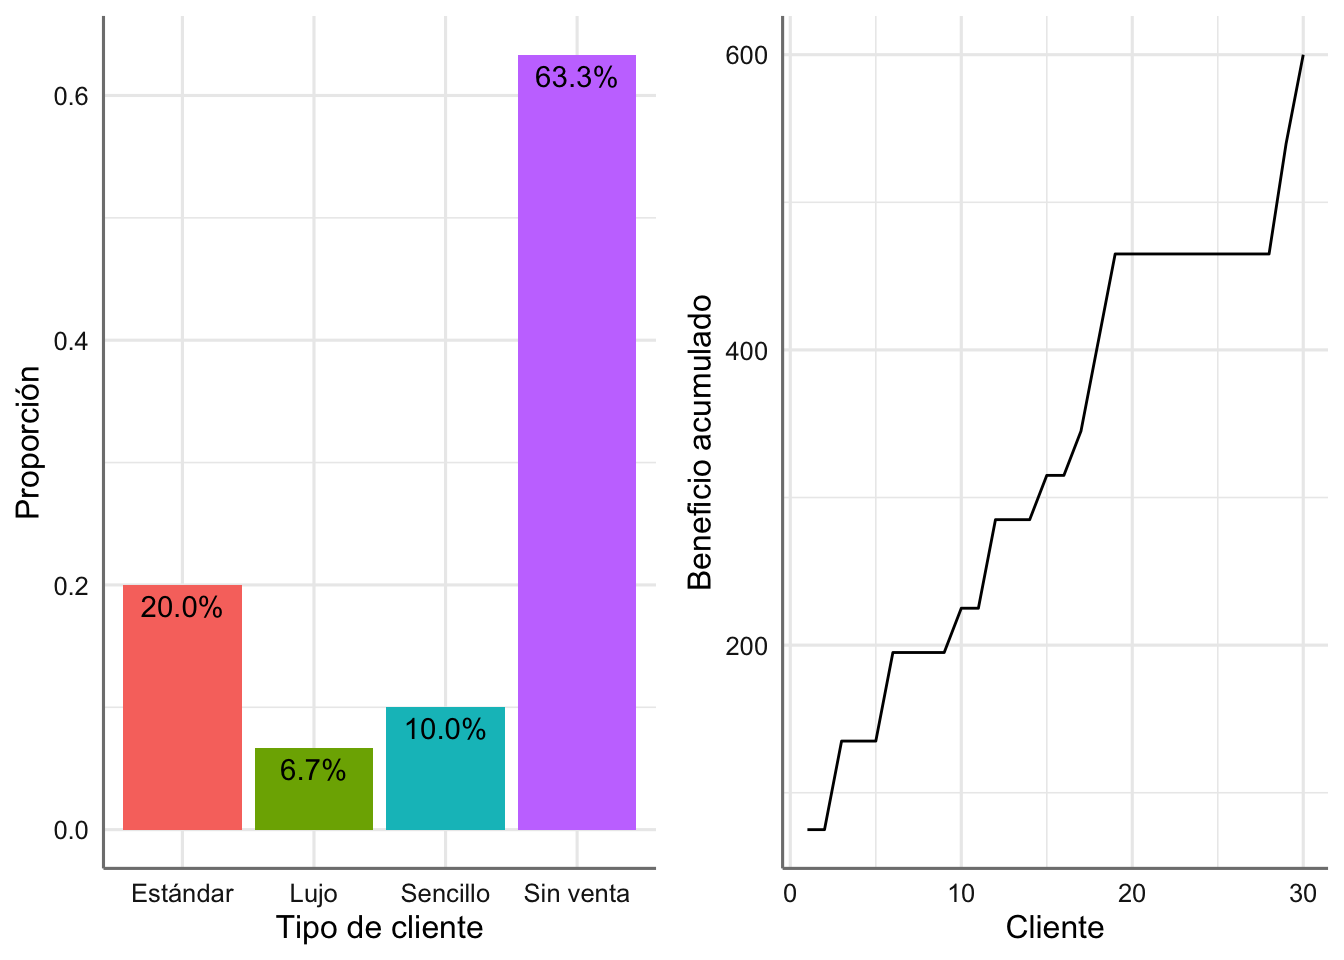
\includegraphics[width=0.95\linewidth]{01-Probabilidad_files/figure-latex/01-025-1} 

}

\caption{Frecuencia relativa de cada tipo de venta (izquierda) y beneficio acumulado para los 30 clientes (derecha).}\label{fig:01-025}
\end{figure}

Podemos también calcular la ganancia promedio que se obtiene con esos 30 clientes a partir de la variable \texttt{simulaciones\$Bind}, que resulta de

\begin{Shaded}
\begin{Highlighting}[]
\FunctionTok{mean}\NormalTok{(simulacion}\SpecialCharTok{$}\NormalTok{Bind)}
\end{Highlighting}
\end{Shaded}

\begin{verbatim}
## [1] 20
\end{verbatim}

Si queremos aproximar el beneficio esperado por cliente, bastará simular muchos clientes, y promediar los beneficios que le dan a la tienda, o incluso el beneficio esperado por cliente que compra un microondas.

\begin{Shaded}
\begin{Highlighting}[]
\NormalTok{nsim }\OtherTok{\textless{}{-}} \DecValTok{1000} \CommentTok{\# número de clientes simulados}
\NormalTok{simulacion }\OtherTok{\textless{}{-}} \FunctionTok{simula.ventas.micro}\NormalTok{(nsim,}\DecValTok{123}\NormalTok{)}
\CommentTok{\# aproximación MC del beneficio medio de un cliente cualquiera}
\FunctionTok{mean}\NormalTok{(simulacion}\SpecialCharTok{$}\NormalTok{Bind)}
\end{Highlighting}
\end{Shaded}

\begin{verbatim}
## [1] 29.025
\end{verbatim}

\begin{Shaded}
\begin{Highlighting}[]
\CommentTok{\# beneficio medio de un cliente de compra}
\FunctionTok{mean}\NormalTok{(simulacion}\SpecialCharTok{$}\NormalTok{Bind[simulacion}\SpecialCharTok{$}\NormalTok{Compra}\SpecialCharTok{==}\StringTok{"Si"}\NormalTok{])}
\end{Highlighting}
\end{Shaded}

\begin{verbatim}
## [1] 57.24852
\end{verbatim}

Así, el beneficio medio por cliente es aproximadamente de 29.03 dólares, mientras que el beneficio esperado por cliente que compra un microondas es de 57.25 dólares. El beneficio esperado por cada 30 clientes que entran en la tienda será de \(20.025 \times 30=870.75\) dólares.

\begin{example}
\protect\hypertarget{exm:mixtura2}{}\label{exm:mixtura2}

Un fabricante de galletas presenta muchos productos nuevos cada año, de los cuales cerca del 60\% fracasan, 30\% tienen un éxito moderado y un 10\% tienen un gran éxito. Para mejorar sus posibilidades, el fabricante somete a una prueba sus nuevos productos, ante un grupo de clientes que actúa como jurado calificador. De los productos que fracasaron, 50\% son calificados como malos, 30\% como regulares y 20\% como buenos. Para los que tuvieron un éxito moderado, la calificación es mala para un 20\%, regular para un 40\% y buena para otro 40\%. Para los que tuvieron un gran éxito, los porcentajes son: malos 10\%, regulares 30\% y buenos 60\%. El fabricante está interesado en conocer:

\begin{itemize}
\item
  ¿Cuál es la probabilidad conjunta de que un producto tenga un éxito moderado y reciba una mala calificación?
\item
  Si un nuevo producto tiene una buena calificación, ¿cuál es la probabilidad de que fracase?
\item
  ¿Cuál es la probabilidad de que un producto tenga éxito moderado dado que este obtuvo una mala calificación?
\end{itemize}

\end{example}

Modelicemos el problema como una mixtura de distribuciones discretas según la Definición \ref{def:mixturadiscreta}.

Sea \(I_i\) la variable indicadora tal que

\begin{equation*}
Pr(I = k) = 
\begin{cases}
0.25 & \text{ para } k = 1 \text{ fracaso}\\
0.50 & \text{ para } k = 2 \text{ éxito moderado}\\
0.25 & \text{ para } k = 3 \text{ gran éxito}.
\end{cases}
\end{equation*}

Luego definimos las variables \(X_i\) que representan la calificación del jurado de un producto cuyo éxito o fracaso funcionó según \(I=i\): \(X_1\) calificación de un producto que fue un fracaso (\(I=1\)), \(X_2\) calificación de un producto con un éxito moderado (\(I=2\)) y \(X_3\) calificación de un producto con una gran éxito (\(I=3\)). Las distribuciones de \(X_1, X_2, X_3\) vienen dadas por:

\begin{equation*}
Pr(X_1 = k) = 
\begin{cases}
0.5 & \text{ para } k = 1 \text{ malo}\\
0.3 & \text{ para } k = 2 \text{ regular}\\
0.2 & \text{ para } k = 3 \text{ bueno}.
\end{cases}
\end{equation*}

\begin{equation*}
Pr(X_2 = k) = 
\begin{cases}
0.2 & \text{ para } k = 1 \text{ malo}\\
0.4 & \text{ para } k = 2 \text{ regular}\\
0.4 & \text{ para } k = 3 \text{ bueno}.
\end{cases}
\end{equation*}

\begin{equation*}
Pr(X_3 = k) = 
\begin{cases}
0.1 & \text{ para } k = 1 \text{ malo}\\
0.3 & \text{ para } k = 2 \text{ regular}\\
0.6 & \text{ para } k = 3 \text{ bueno}.
\end{cases}
\end{equation*}

Veamos el algoritmo de simulación necesario para este problema. Queremos simular productos que pueden haber tenido un gran éxito, un éxito moderado y o haber fracasado. Y para cada uno de ellos, queremos simular su calificación por el jurado que lo evaluó.

\begin{silverbox}

Consideramos una variable \(I\) que indica el éxito de un nuevo producto y \(X_I\) que indica la evaluación del producto por un jurado (para cada tipo de producto \(I\)). En esta situación debemos proporcionar las simulaciones correspondientes a \(I\) e \(X_I\). En concreto:

\begin{itemize}
\tightlist
\item
  Paso 1. Establecer tamaño de muestra a simular \(nsim\).
\end{itemize}

Repetir los pasos 2 y 3 para cada iteración \(i\) de \(1, 2,..., nsim\):

\begin{itemize}
\item
  Paso 2. Simular de la variable indicador, \(I_i\), mediante el algoritmo de la transformada inversa para una variable discreta con probabilidades \(0.6, 0.3, 0.1\) (fracaso, éxito moderado, gran éxito), y seleccionar la variable \(X_{I_i}\).
\item
  Paso 3. Simular un valor \(x_{I_i}\) mediante el algoritmo de la transformada inversa para \(X_i\) con valores malos, regulares, buenos, y probabilidades dadas por:

  \begin{itemize}
  \tightlist
  \item
    fracasos (0.5, 0.3, 0.2)
  \item
    éxito moderado (0.2, 0.4, 0.4)
  \item
    gran éxito (0.1, 0.3, 0.6)
  \end{itemize}
\item
  Paso 4. Devolver el conjunto de simulaciones \(\{(I_i, x_{I_i})\}_{i=1}^{nsim}.\)
\end{itemize}

\end{silverbox}

Procedamos pues, a simular el proceso para, con las simulaciones, responder a las preguntas planteadas por la empresa.

\begin{Shaded}
\begin{Highlighting}[]
\CommentTok{\# Parámetros iniciales}
\NormalTok{nsim }\OtherTok{\textless{}{-}} \DecValTok{5000}
\NormalTok{semilla }\OtherTok{\textless{}{-}} \DecValTok{12}
\CommentTok{\# Descripción variable indicadora}
\NormalTok{exito }\OtherTok{\textless{}{-}} \FunctionTok{c}\NormalTok{(}\StringTok{"Fracaso"}\NormalTok{, }\StringTok{"Moderado"}\NormalTok{, }\StringTok{"Éxito"}\NormalTok{)}
\NormalTok{pexito }\OtherTok{\textless{}{-}} \FunctionTok{c}\NormalTok{(}\FloatTok{0.6}\NormalTok{, }\FloatTok{0.3}\NormalTok{, }\FloatTok{0.1}\NormalTok{)}
\NormalTok{pexitoacum }\OtherTok{\textless{}{-}} \FunctionTok{cumsum}\NormalTok{(pexito)}
\CommentTok{\# Descripción del proceso de adquisión del microondas}
\NormalTok{clasifi }\OtherTok{\textless{}{-}} \FunctionTok{c}\NormalTok{(}\StringTok{"Malo"}\NormalTok{, }\StringTok{"Regular"}\NormalTok{, }\StringTok{"Bueno"}\NormalTok{)}
\NormalTok{p1 }\OtherTok{\textless{}{-}} \FunctionTok{c}\NormalTok{(}\FloatTok{0.5}\NormalTok{, }\FloatTok{0.3}\NormalTok{, }\FloatTok{0.2}\NormalTok{)}
\NormalTok{p2 }\OtherTok{\textless{}{-}} \FunctionTok{c}\NormalTok{(}\FloatTok{0.2}\NormalTok{, }\FloatTok{0.4}\NormalTok{, }\FloatTok{0.4}\NormalTok{)}
\NormalTok{p3 }\OtherTok{\textless{}{-}} \FunctionTok{c}\NormalTok{(}\FloatTok{0.1}\NormalTok{, }\FloatTok{0.3}\NormalTok{, }\FloatTok{0.6}\NormalTok{)}
\NormalTok{p1acum }\OtherTok{\textless{}{-}} \FunctionTok{cumsum}\NormalTok{(p1)}
\NormalTok{p2acum }\OtherTok{\textless{}{-}} \FunctionTok{cumsum}\NormalTok{(p2)}
\NormalTok{p3acum }\OtherTok{\textless{}{-}} \FunctionTok{cumsum}\NormalTok{(p3)}

\CommentTok{\# Inicialización de variables para las simulaciones}
\NormalTok{producto }\OtherTok{\textless{}{-}} \FunctionTok{c}\NormalTok{()             }\CommentTok{\# éxito producto}
\NormalTok{jurado }\OtherTok{\textless{}{-}} \FunctionTok{c}\NormalTok{()               }\CommentTok{\# clasificación jurado}

\DocumentationTok{\#\# Simulación del proceso}
\DocumentationTok{\#\#\#\#\#\#\#\#\#\#\#\#\#\#\#\#\#\#\#\#\#\#\#\#\#\#}
\NormalTok{i }\OtherTok{\textless{}{-}} \DecValTok{1}
\CommentTok{\# Generamos uniformes para describir el proceso de indicadores de éxito}
\CommentTok{\# y también el de evaluación o clasificación por el jurado}
\FunctionTok{set.seed}\NormalTok{(semilla)}
\NormalTok{uexito }\OtherTok{\textless{}{-}} \FunctionTok{runif}\NormalTok{(nsim)  }
\NormalTok{uclasi }\OtherTok{\textless{}{-}} \FunctionTok{runif}\NormalTok{(nsim)}

\CommentTok{\# Bucle de simulación}
\ControlFlowTok{while}\NormalTok{ (i }\SpecialCharTok{\textless{}=}\NormalTok{ nsim)}
\NormalTok{\{}
  \CommentTok{\# Éxito del producto}
\NormalTok{  producto[i] }\OtherTok{\textless{}{-}}\NormalTok{ exito[}\FunctionTok{min}\NormalTok{(}\FunctionTok{which}\NormalTok{(uexito[i] }\SpecialCharTok{\textless{}=}\NormalTok{ pexitoacum))]}
  \CommentTok{\# Tipo de microndas}
  \ControlFlowTok{if}\NormalTok{(producto[i] }\SpecialCharTok{==}\NormalTok{ exito[}\DecValTok{1}\NormalTok{])}
\NormalTok{  \{}
\NormalTok{    jurado[i] }\OtherTok{\textless{}{-}}\NormalTok{ clasifi[}\FunctionTok{min}\NormalTok{(}\FunctionTok{which}\NormalTok{(uclasi[i] }\SpecialCharTok{\textless{}=}\NormalTok{ p1acum))]}
\NormalTok{  \}}
  \ControlFlowTok{else} \ControlFlowTok{if}\NormalTok{ (producto[i] }\SpecialCharTok{==}\NormalTok{ exito[}\DecValTok{2}\NormalTok{])}
\NormalTok{  \{}
\NormalTok{    jurado[i] }\OtherTok{\textless{}{-}}\NormalTok{ clasifi[}\FunctionTok{min}\NormalTok{(}\FunctionTok{which}\NormalTok{(uclasi[i] }\SpecialCharTok{\textless{}=}\NormalTok{ p2acum))]}
\NormalTok{  \}}
  \ControlFlowTok{else}
\NormalTok{  \{}
\NormalTok{    jurado[i] }\OtherTok{\textless{}{-}}\NormalTok{ clasifi[}\FunctionTok{min}\NormalTok{(}\FunctionTok{which}\NormalTok{(uclasi[i] }\SpecialCharTok{\textless{}=}\NormalTok{ p3acum))]    }
\NormalTok{  \}}
  \CommentTok{\# nueva simulación}
\NormalTok{  i }\OtherTok{\textless{}{-}}\NormalTok{ i}\SpecialCharTok{+}\DecValTok{1}
\NormalTok{\}}
\CommentTok{\# Resultado}
\NormalTok{simulacion }\OtherTok{\textless{}{-}} \FunctionTok{data.frame}\NormalTok{(}\AttributeTok{producto =}\NormalTok{ producto, }\AttributeTok{jurado =}\NormalTok{ jurado)}
\end{Highlighting}
\end{Shaded}

A partir de las simulaciones, obtenemos la tabla conjunta de frecuencias (Tabla \ref{tab:01-030a}) y las frecuencias relativas (Tabla \ref{tab:01-030b}), que constituyen una aproximación de las probabilidades de ocurrencia.

\begin{Shaded}
\begin{Highlighting}[]
\NormalTok{distri.conjunta.frec }\OtherTok{\textless{}{-}} \FunctionTok{table}\NormalTok{(simulacion)}
\FunctionTok{kbl}\NormalTok{(distri.conjunta.frec,}\AttributeTok{caption=}\StringTok{"Frecuencias observadas en las simulaciones."}\NormalTok{) }\SpecialCharTok{\%\textgreater{}\%}
  \FunctionTok{kable\_styling}\NormalTok{(}\AttributeTok{bootstrap\_options =} \FunctionTok{c}\NormalTok{(}\StringTok{"striped"}\NormalTok{, }\StringTok{"hover"}\NormalTok{),}\AttributeTok{full\_width =}\NormalTok{ F)}
\end{Highlighting}
\end{Shaded}

\begin{table}

\caption{\label{tab:01-030a}Frecuencias observadas en las simulaciones.}
\centering
\begin{tabular}[t]{l|r|r|r}
\hline
  & Bueno & Malo & Regular\\
\hline
Éxito & 327 & 47 & 166\\
\hline
Fracaso & 650 & 1516 & 844\\
\hline
Moderado & 616 & 292 & 542\\
\hline
\end{tabular}
\end{table}

\begin{Shaded}
\begin{Highlighting}[]
\NormalTok{distri.conjunta}\OtherTok{=}\FunctionTok{as.data.frame}\NormalTok{(}\FunctionTok{table}\NormalTok{(simulacion)}\SpecialCharTok{/}\NormalTok{nsim)}
\FunctionTok{kbl}\NormalTok{(distri.conjunta,}\AttributeTok{caption=}\StringTok{"Frecuencias relativas observadas en las simulaciones. Aproximación de la distribución conjunta."}\NormalTok{) }\SpecialCharTok{\%\textgreater{}\%}
    \FunctionTok{kable\_styling}\NormalTok{(}\AttributeTok{bootstrap\_options =} \FunctionTok{c}\NormalTok{(}\StringTok{"striped"}\NormalTok{, }\StringTok{"hover"}\NormalTok{),}\AttributeTok{full\_width =}\NormalTok{ F)}
\end{Highlighting}
\end{Shaded}

\begin{table}

\caption{\label{tab:01-030b}Frecuencias relativas observadas en las simulaciones. Aproximación de la distribución conjunta.}
\centering
\begin{tabular}[t]{l|l|r}
\hline
producto & jurado & Freq\\
\hline
Éxito & Bueno & 0.0654\\
\hline
Fracaso & Bueno & 0.1300\\
\hline
Moderado & Bueno & 0.1232\\
\hline
Éxito & Malo & 0.0094\\
\hline
Fracaso & Malo & 0.3032\\
\hline
Moderado & Malo & 0.0584\\
\hline
Éxito & Regular & 0.0332\\
\hline
Fracaso & Regular & 0.1688\\
\hline
Moderado & Regular & 0.1084\\
\hline
\end{tabular}
\end{table}

Podemos contestar ahora a las preguntas planteadas sin más que mirar la tabla anterior o realizar calculos sencillos con los datos obtenidos:

\begin{itemize}
\tightlist
\item
  ¿Cuál es la probabilidad conjunta de que un producto tenga un éxito moderado y reciba una mala calificación? Estamos interesados en la probabilidad
\end{itemize}

\[Pr(\text{Éxito = "Moderado" y Evaluación =  "Malo"})\]

cuyo valor es 0.0584.

\begin{itemize}
\tightlist
\item
  Si un nuevo producto tiene una buena calificación, ¿cuál es la probabilidad de que fracase? Para responder a esta pregunta podemos aplicar el Teorema de Bayes para resolver la probabilidad condicionada siguiente a partir de las frecuencias observadas en la simulación y mostradas en la Tabla \ref{tab:01-030a},
\end{itemize}

\[Pr(\text{E= "Fracaso" | Eval= "Bueno"}) =
\frac{Pr(\text{ E="Fracaso" , Eval= "Bueno"})}{Pr(\text{ Eval= "Bueno"})}\]

donde \(E=\)Éxito y \(Eval=\)Evaluación,

\begin{Shaded}
\begin{Highlighting}[]
\NormalTok{distri.conjunta.frec[}\DecValTok{2}\NormalTok{,}\DecValTok{1}\NormalTok{]}\SpecialCharTok{/}\FunctionTok{sum}\NormalTok{(distri.conjunta.frec[,}\DecValTok{1}\NormalTok{])}
\end{Highlighting}
\end{Shaded}

\begin{verbatim}
## [1] 0.4080352
\end{verbatim}

o directamente seleccionar sobre la Tabla \ref{tab:01-030b} las simulaciones en las que el producto fue evaluado como ``Bueno'' por el jurado, y contabilizar en cuántas de ellas el producto finalmente fracasó (a través del ratio correspondiente).

\begin{Shaded}
\begin{Highlighting}[]
\NormalTok{distri.conjunta }\SpecialCharTok{\%\textgreater{}\%} 
  \FunctionTok{filter}\NormalTok{(jurado }\SpecialCharTok{==} \StringTok{"Bueno"}\NormalTok{) }\SpecialCharTok{\%\textgreater{}\%}
  \FunctionTok{mutate}\NormalTok{(}\AttributeTok{pr.bueno =} \FunctionTok{sum}\NormalTok{(Freq), }\AttributeTok{resultado =} \FunctionTok{round}\NormalTok{(Freq}\SpecialCharTok{/}\NormalTok{pr.bueno,}\DecValTok{4}\NormalTok{)) }\SpecialCharTok{\%\textgreater{}\%}
  \FunctionTok{kbl}\NormalTok{(}\AttributeTok{caption=}\StringTok{"Distribución condicionada a que el producto fue evaluado como Bueno por el jurado."}\NormalTok{)}\SpecialCharTok{\%\textgreater{}\%}
      \FunctionTok{kable\_styling}\NormalTok{(}\AttributeTok{bootstrap\_options =}\FunctionTok{c}\NormalTok{(}\StringTok{"striped"}\NormalTok{,}\StringTok{"hoover"}\NormalTok{),}\AttributeTok{full\_width =}\NormalTok{ F)}
\end{Highlighting}
\end{Shaded}

\begin{table}

\caption{\label{tab:01-031}Distribución condicionada a que el producto fue evaluado como Bueno por el jurado.}
\centering
\begin{tabular}[t]{l|l|r|r|r}
\hline
producto & jurado & Freq & pr.bueno & resultado\\
\hline
Éxito & Bueno & 0.0654 & 0.3186 & 0.2053\\
\hline
Fracaso & Bueno & 0.1300 & 0.3186 & 0.4080\\
\hline
Moderado & Bueno & 0.1232 & 0.3186 & 0.3867\\
\hline
\end{tabular}
\end{table}

La probabilidad de interés resulta 0.4080. De hecho, en la Tabla \ref{tab:01-031} se muestran, en la columna ``resultado'', las probabilidades condicionadas a que el jurado emitió una buena calificación del producto. ¿Cómo podemos interpretar esas probabilidades?

\begin{itemize}
\tightlist
\item
  ¿Cuál es la probabilidad de que un producto tenga éxito moderado dado que éste obtuvo una mala calificación? Procedemos como en la pregunta anterior ya que estamos interesados en
\end{itemize}

\[Pr(\text{E= "Moderado" | Eval = "Malo"}) = \frac{Pr(\text{E= "Moderado" , Eval = "Malo"})}{Pr(\text{ Eval= "Malo"})}\]

y lo resolvemos de nuevo generando la distribución condicionada a que la evaluación por el jurado sea ``Mala'', que se muestra en la Tabla \ref{tab:01-032}

\begin{Shaded}
\begin{Highlighting}[]
\NormalTok{distri.conjunta }\SpecialCharTok{\%\textgreater{}\%} 
  \FunctionTok{filter}\NormalTok{(jurado }\SpecialCharTok{==} \StringTok{"Malo"}\NormalTok{) }\SpecialCharTok{\%\textgreater{}\%}
  \FunctionTok{mutate}\NormalTok{(}\AttributeTok{pr.malo =} \FunctionTok{sum}\NormalTok{(Freq), }\AttributeTok{resultado =} \FunctionTok{round}\NormalTok{(Freq}\SpecialCharTok{/}\NormalTok{pr.malo,}\DecValTok{4}\NormalTok{)) }\SpecialCharTok{\%\textgreater{}\%}
  \FunctionTok{kbl}\NormalTok{(}\AttributeTok{caption=}\StringTok{"Distribución condicionada a que el producto fue evaluado como Malo por el jurado."}\NormalTok{) }\SpecialCharTok{\%\textgreater{}\%}
  \FunctionTok{kable\_styling}\NormalTok{(}\AttributeTok{bootstrap\_options =}\FunctionTok{c}\NormalTok{(}\StringTok{"striped"}\NormalTok{,}\StringTok{"hoover"}\NormalTok{),}\AttributeTok{full\_width =}\NormalTok{ F)}
\end{Highlighting}
\end{Shaded}

\begin{table}

\caption{\label{tab:01-032}Distribución condicionada a que el producto fue evaluado como Malo por el jurado.}
\centering
\begin{tabular}[t]{l|l|r|r|r}
\hline
producto & jurado & Freq & pr.malo & resultado\\
\hline
Éxito & Malo & 0.0094 & 0.371 & 0.0253\\
\hline
Fracaso & Malo & 0.3032 & 0.371 & 0.8173\\
\hline
Moderado & Malo & 0.0584 & 0.371 & 0.1574\\
\hline
\end{tabular}
\end{table}

La probabilidad de interés es 0.1574. ¿Cómo podemos interpretar la Tabla \ref{tab:01-032} de probabilidades obtenida?

\hypertarget{otras-distribuciones-continuas}{%
\section{Otras distribuciones continuas}\label{otras-distribuciones-continuas}}

En el caso de variables de tipo continuo de las que no disponemos de un generador de valores aleatorios pero sí disponemos de su función de densidad o distribución, podemos utilizar el algoritmo de la transformada inversa, dado en la definición \ref{def:aticontinua}, para obtener una muestra aleatoria de tamaño \(n\) de su distribución.

En primer lugar estudiamos situaciones con una variable y posteriormente vemos ejemplos de sistemas de variables continuas o mixturas de discretas y continuas.

\hypertarget{una-variable-continua}{%
\subsection{Una variable continua}\label{una-variable-continua}}

Estudiamos aquí, a través de ejemplos, la simulación de variables aleatorias de tipo continua para las que conocemos la función de densidad o distribución, y se quiere revolver algún problema inferencial.

\begin{example}
\protect\hypertarget{exm:cont1}{}\label{exm:cont1}

Sea \(X\) una variable aleatoria de tipo continuo cuya función de densidad viene dada por:

\begin{equation*}
f(x) = 2e^{-2x}  \text{ para } x \geq 0
\end{equation*}

Estamos interesados en conocer:

\begin{itemize}
\tightlist
\item
  ¿Cuál es la probabilidad de que la variable de interés tome valores en el intervalo {[}1, 2{]}?
\item
  ¿Cuál es la probabilidad de que la variable de interés tome valores mayores o iguales a 1.5?
\item
  ¿Cuál es el valor esperado de la variable? ¿y la desviación típica?
\end{itemize}

\end{example}

Para poder responder a las preguntas planteadas debemos obtener en primer lugar la función de distribución asociada a \(X\), que viene dada por:

\begin{equation}
F(x) = \int_0^x 2e^{-2s} ds=1 - e^{-2x} \text{ para } x \geq 0
\label{eq:fd1-16}
\end{equation}

Podemos aplicar ahora el método de la transformada inversa para obtener una muestra de \(X\).

El algoritmo de simulación basado en la transformada inversa, en la Definición \ref{def:aticontinua} viene dado por:

\begin{silverbox}

Si \(F(X)\) es la función de distribución para \(X\) dada en la Ecuación \eqref{eq:fd1-16}

\begin{itemize}
\tightlist
\item
  Paso 1. Establecer el tamaño de muestra a simular \(nsim\).
\end{itemize}

Repetir los pasos 2 y 3 para cada iteración \(i\) de \(1, 2,..., nsim\):

\begin{itemize}
\item
  Paso 2. Generar \(u_i\) a partir de una \(U(0,1)\).
\item
  Paso 3. Aplicar el método de la transformada inversa para obtener \(x_i = F^{-1}(u_i)\) con \(F^{1}(u_i) = -log(1-u_i)/2.\)
\item
  Paso 4. Devolver el conjunto de simulaciones \(\{x_i\}_{i=1}^{nsim}\).
\end{itemize}

\end{silverbox}

Apliquemos pues el algoritmo anterior, y generemos una muestra de tamaño \(nsim=5000\) para \(X\). Aprovechamos el calculo vectorial de \texttt{R} para no tener que hacer un bucle.

\begin{Shaded}
\begin{Highlighting}[]
\CommentTok{\# Parámetros iniciales}
\NormalTok{nsim }\OtherTok{\textless{}{-}} \DecValTok{5000}
\FunctionTok{set.seed}\NormalTok{(}\DecValTok{12}\NormalTok{)}
\CommentTok{\# Generamos uniformes }
\NormalTok{uniforme }\OtherTok{\textless{}{-}} \FunctionTok{runif}\NormalTok{(nsim)}
\CommentTok{\# Calculamos x con F\^{}{-}1}
\NormalTok{xs }\OtherTok{\textless{}{-}} \SpecialCharTok{{-}}\FunctionTok{log}\NormalTok{(}\DecValTok{1}\SpecialCharTok{{-}}\NormalTok{uniforme)}\SpecialCharTok{/}\DecValTok{2}
\end{Highlighting}
\end{Shaded}

Y con las simulaciones obtenidas, respondamos a cada una de las preguntas planteadas:

\begin{Shaded}
\begin{Highlighting}[]
\CommentTok{\# Pr(1 \textless{}= X \textless{}= 2)}
\FunctionTok{cat}\NormalTok{(}\StringTok{"Pr(1 \textless{}= X \textless{}= 2)="}\NormalTok{,}\FunctionTok{round}\NormalTok{(}\FunctionTok{mean}\NormalTok{(xs }\SpecialCharTok{\textgreater{}=} \DecValTok{1} \SpecialCharTok{\&}\NormalTok{ xs }\SpecialCharTok{\textless{}=} \DecValTok{2}\NormalTok{), }\DecValTok{4}\NormalTok{))}
\end{Highlighting}
\end{Shaded}

\begin{verbatim}
## Pr(1 <= X <= 2)= 0.121
\end{verbatim}

\begin{Shaded}
\begin{Highlighting}[]
\CommentTok{\# Pr(X \textgreater{}= 1.5)}
\FunctionTok{cat}\NormalTok{(}\StringTok{"Pr(X \textgreater{}= 1.5)="}\NormalTok{,}\FunctionTok{round}\NormalTok{(}\FunctionTok{mean}\NormalTok{(xs }\SpecialCharTok{\textgreater{}=} \FloatTok{1.5}\NormalTok{), }\DecValTok{4}\NormalTok{))}
\end{Highlighting}
\end{Shaded}

\begin{verbatim}
## Pr(X >= 1.5)= 0.053
\end{verbatim}

\begin{Shaded}
\begin{Highlighting}[]
\CommentTok{\# Valor esperado y varianza}
\FunctionTok{cat}\NormalTok{(}\StringTok{"E(X)="}\NormalTok{,}\FunctionTok{round}\NormalTok{(}\FunctionTok{mean}\NormalTok{(xs), }\DecValTok{4}\NormalTok{))}
\end{Highlighting}
\end{Shaded}

\begin{verbatim}
## E(X)= 0.5046
\end{verbatim}

\begin{Shaded}
\begin{Highlighting}[]
\FunctionTok{cat}\NormalTok{(}\StringTok{"V(X)="}\NormalTok{,}\FunctionTok{round}\NormalTok{(}\FunctionTok{sd}\NormalTok{(xs), }\DecValTok{4}\NormalTok{))}
\end{Highlighting}
\end{Shaded}

\begin{verbatim}
## V(X)= 0.5078
\end{verbatim}

\hypertarget{composicionsec}{%
\subsection{Transformaciones y Método de Composición}\label{composicionsec}}

En ocasiones, se nos plantea el problema de inferir, a través de simulación, sobre una variable aleatoria \(Y\) que se obtiene como una transformación continua de otra variable \(X\) cuya distribución conocemos, esto es, \[Y=h(X), \quad \text{ con } X \sim F(x).\]

En particular, \[E(Y)=\int_S h(x) f(x)dx.\]

Se propone un algoritmo sencillo para simular muestras aleatorias de la variable \(Y\), denominado \textbf{método de composición} y que se presenta a continuación.

\begin{yellowbox}

\begin{definition}
\protect\hypertarget{def:metodocomposicion}{}\label{def:metodocomposicion}

\textbf{Método de composición}

Si \(X\) es una variable aleatoria continua con función de distribución \(F(X)\), e \(Y\) otra variable aleatoria que se obtiene como \(Y = h(X)\), donde \(h()\) es una función continua, podemos obtener una muestra de \(Y\) a partir del siguiente proceso:

\begin{itemize}
\tightlist
\item
  Paso 1. Fijar el número de simulaciones (\(nsim\)).
\end{itemize}

Repetir los pasos 2 y 3 hasta alcanzar el número de simulaciones del paso 1.

\begin{itemize}
\tightlist
\item
  Paso 2. Generar un valor de la variable \(X\), \(\{x_i \sim F(x)\}\).\\
\item
  Paso 3. Calcular el valor de la variable \(Y\) para esa simulación mediante \(y_i = h(x_i)\).
\item
  Paso 4. Devolver el conjunto de valores simulados \(\{y_i\}_{i=1}^{nsim}.\)
\end{itemize}

\end{definition}

\end{yellowbox}

\begin{example}
\protect\hypertarget{exm:cont2}{}\label{exm:cont2}

Sea \(X\) una variable aleatoria de tipo continuo cuya función de densidad viene dada por:

\begin{equation*}
f(x) = 3x^2  \text{ para } 0 < x < 1
\end{equation*}

y consideramos la variable aleatoria \(Y = 1 - X^2\). Estamos interesados en conocer:

\begin{itemize}
\tightlist
\item
  ¿Cuál es el valor esperado de la variable \(Y\)? ¿Y su desviación típica?
\item
  \(Pr(Y \in [0,1])\)
\item
  \(Pr(Y \geq 0.5)\)
\end{itemize}

\end{example}

Puesto que la distribución de \(X\) no es de las estándar, para simular de ella hemos de utilizar el método de la transformada inversa (Definición \ref{def:aticontinua}), para lo que hemos de obtener necesariamente su función de distribución, que viene dada por:

\begin{equation}
F(x) = 
\begin{cases}
0 & \text{ para } x <= 0\\
x^3 & \text{ para } 0 < x < 1\\
1 & \text{ para } x \geq 1
\end{cases}
\label{eq:fdx2}
\end{equation}

La función de distribución inversa es pues: \[F^{-1}(u)=u^{1/3}\]

El algoritmo para obtener una muestra de \(Y\) viene dado por:

\begin{silverbox}

Si \(F(X)\) es la función de distribución para \(X\) dada en \eqref{eq:fdx2}

\begin{itemize}
\tightlist
\item
  Paso 1. Establecer tamaño de muestra a simular \(nsim\).
\end{itemize}

Repetir los pasos 2 a 4 para cada iteración \(i\) de \(1, 2,..., nsim\):

\begin{itemize}
\tightlist
\item
  Paso 2. Generar \(u_i\) a partir de una \(U(0,1)\).
\item
  Paso 3. Aplicar el método de la transformada inversa para obtener \(x_i = F^{-1}(u_i)=u^{1/3}\).
\item
  Paso 4. Actuar por composición y calcular \(y_i = 1 - x_i^2\).
\item
  Paso 5. Devolver el conjunto \(\{y_i\}_{i=1}^{nsim}.\)
\end{itemize}

\end{silverbox}

Procedemos con el algoritmo de simulación.

\begin{Shaded}
\begin{Highlighting}[]
\CommentTok{\# Parámetros iniciales}
\NormalTok{nsim }\OtherTok{\textless{}{-}} \DecValTok{5000}
\FunctionTok{set.seed}\NormalTok{(}\DecValTok{12}\NormalTok{)}
\CommentTok{\# Generamos uniformes }
\NormalTok{uniforme }\OtherTok{\textless{}{-}} \FunctionTok{runif}\NormalTok{(nsim)}
\CommentTok{\# Calculamos x con F\^{}{-}1}
\NormalTok{xs }\OtherTok{\textless{}{-}}\NormalTok{ uniforme}\SpecialCharTok{\^{}}\NormalTok{(}\DecValTok{1}\SpecialCharTok{/}\DecValTok{3}\NormalTok{)}
\CommentTok{\# Calculamos y = h(x)}
\NormalTok{ys }\OtherTok{\textless{}{-}} \DecValTok{1} \SpecialCharTok{{-}}\NormalTok{ xs}
\CommentTok{\# Devolvemos los valores de x e y}
\NormalTok{simulacion }\OtherTok{\textless{}{-}} \FunctionTok{data.frame}\NormalTok{(}\AttributeTok{sim =} \DecValTok{1}\SpecialCharTok{:}\NormalTok{nsim, }\AttributeTok{x =}\NormalTok{ xs, }\AttributeTok{y =}\NormalTok{ ys)}
\end{Highlighting}
\end{Shaded}

Podemos calcular ahora las cantidades de interés:

\begin{Shaded}
\begin{Highlighting}[]
\CommentTok{\# Valor esperado y desviación típica de Y }
\NormalTok{datos }\OtherTok{\textless{}{-}}\NormalTok{ simulacion}\SpecialCharTok{$}\NormalTok{y}
\FunctionTok{cat}\NormalTok{(}\StringTok{"E(Y)="}\NormalTok{, }\FunctionTok{round}\NormalTok{(}\FunctionTok{mean}\NormalTok{(datos), }\DecValTok{4}\NormalTok{))}
\end{Highlighting}
\end{Shaded}

\begin{verbatim}
## E(Y)= 0.2478
\end{verbatim}

\begin{Shaded}
\begin{Highlighting}[]
\FunctionTok{cat}\NormalTok{(}\StringTok{"sd(Y)="}\NormalTok{, }\FunctionTok{round}\NormalTok{(}\FunctionTok{sd}\NormalTok{(datos), }\DecValTok{4}\NormalTok{))}
\end{Highlighting}
\end{Shaded}

\begin{verbatim}
## sd(Y)= 0.1915
\end{verbatim}

\begin{Shaded}
\begin{Highlighting}[]
\CommentTok{\# Pr(0 \textless{}= Y \textless{}= 1) }
\FunctionTok{cat}\NormalTok{(}\StringTok{"Pr(0 \textless{}= Y \textless{}= 1)="}\NormalTok{, }\FunctionTok{round}\NormalTok{(}\FunctionTok{sum}\NormalTok{(datos }\SpecialCharTok{\textgreater{}=} \DecValTok{0} \SpecialCharTok{\&}\NormalTok{ datos }\SpecialCharTok{\textless{}=} \DecValTok{1}\NormalTok{)}\SpecialCharTok{/}\NormalTok{nsim, }\DecValTok{4}\NormalTok{))}
\end{Highlighting}
\end{Shaded}

\begin{verbatim}
## Pr(0 <= Y <= 1)= 1
\end{verbatim}

\begin{Shaded}
\begin{Highlighting}[]
\CommentTok{\# Pr(Y \textgreater{}= 1) }
\FunctionTok{cat}\NormalTok{(}\StringTok{"Pr(Y \textgreater{}= 0.5)="}\NormalTok{, }\FunctionTok{round}\NormalTok{(}\FunctionTok{sum}\NormalTok{(datos }\SpecialCharTok{\textgreater{}=} \FloatTok{0.5}\NormalTok{)}\SpecialCharTok{/}\NormalTok{nsim, }\DecValTok{4}\NormalTok{))}
\end{Highlighting}
\end{Shaded}

\begin{verbatim}
## Pr(Y >= 0.5)= 0.121
\end{verbatim}

Representamos gráficamente las simulaciones obtenidas tanto para la variable \(X\) como la \(Y\).

\begin{Shaded}
\begin{Highlighting}[]
\NormalTok{g1 }\OtherTok{\textless{}{-}} \FunctionTok{ggplot}\NormalTok{(simulacion, }\FunctionTok{aes}\NormalTok{(x, ..density..)) }\SpecialCharTok{+} 
  \FunctionTok{geom\_histogram}\NormalTok{(}\AttributeTok{fill =} \StringTok{"steelblue"}\NormalTok{) }\SpecialCharTok{+}
  \FunctionTok{geom\_density}\NormalTok{()}\SpecialCharTok{+}
  \FunctionTok{labs}\NormalTok{(}\AttributeTok{x =} \StringTok{"X"}\NormalTok{, }\AttributeTok{y =} \StringTok{"Densidad"}\NormalTok{)}
\NormalTok{g2 }\OtherTok{\textless{}{-}} \FunctionTok{ggplot}\NormalTok{(simulacion, }\FunctionTok{aes}\NormalTok{(y, ..density..)) }\SpecialCharTok{+} 
  \FunctionTok{geom\_histogram}\NormalTok{(}\AttributeTok{fill =} \StringTok{"steelblue"}\NormalTok{) }\SpecialCharTok{+}
  \FunctionTok{geom\_density}\NormalTok{()}\SpecialCharTok{+}
  \FunctionTok{labs}\NormalTok{(}\AttributeTok{x =} \StringTok{"Y"}\NormalTok{, }\AttributeTok{y =} \StringTok{"Densidad"}\NormalTok{)}
\FunctionTok{grid.arrange}\NormalTok{(g1, g2, }\AttributeTok{nrow =} \DecValTok{1}\NormalTok{)}
\end{Highlighting}
\end{Shaded}

\begin{verbatim}
## `stat_bin()` using `bins = 30`. Pick better value with `binwidth`.
## `stat_bin()` using `bins = 30`. Pick better value with `binwidth`.
\end{verbatim}

\begin{figure}

{\centering 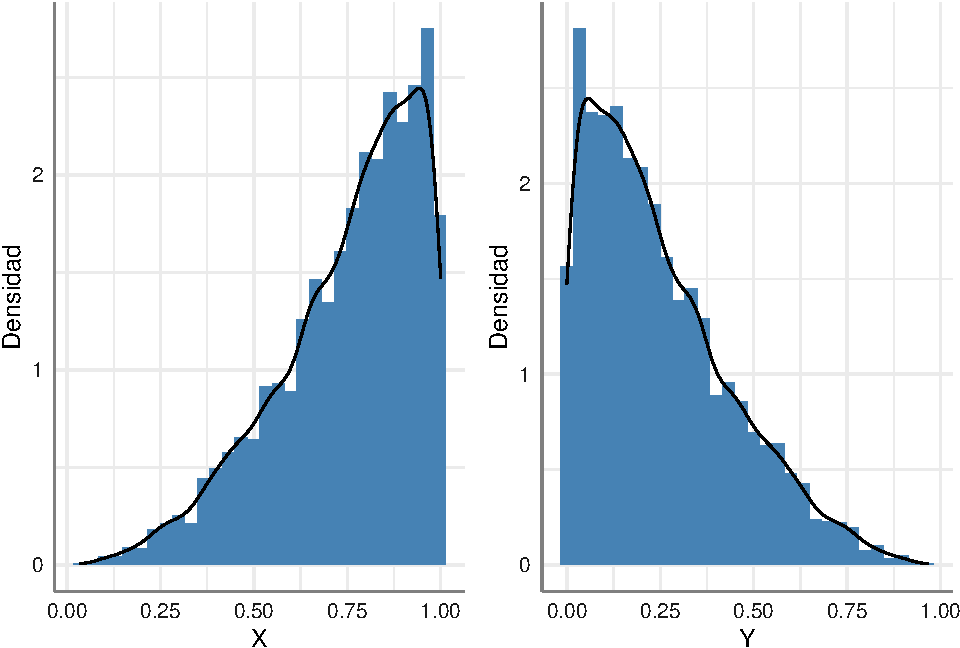
\includegraphics[width=0.95\linewidth]{01-Probabilidad_files/figure-latex/01-037-1} 

}

\caption{Función de densidad empírica e histogramas para X e Y.}\label{fig:01-037}
\end{figure}

\hypertarget{combinaciones-de-variables}{%
\subsection{Combinaciones de variables}\label{combinaciones-de-variables}}

Continuamos este bloque con un tipo de problema que nos encontraremos en muchas ocasiones en el análisis de sistemas, como es la definición de nuevas variables al operar (combinar aritméticamente) otras cuya distribución es conocida. Un ejemplo típico es la suma o resta de variables aleatorias. Imaginemos que tenemos dos variables \(X_1\) y \(X_2\) con funciones de densidad \(f_1(x_1)\) y \(f_2(x_2)\) respectivamente, y estamos interesados en estudiar las variables:

\[Y = X_1 + X_2 \quad\text{ y } \quad Z = X_1 - X_2\] Para el estudio de \(Y\) y \(Z\) podemos proceder teóricamente mediante los correspondientes cambios de variable, pero en situaciones má complejas o con más variables ese procedimiento es poco práctico. En dichas situaciones, podemos utilizar el método de composición para obtener una muestra de las nuevas variables.

\begin{yellowbox}

\begin{definition}

\textbf{Método de composición para combinaciones de variables}

Si \(X_1,..., X_n\) es un conjunto de variables aleatorias continuas con funciones de distribución \(F_1,..., F_n\) y se define la variable aleatoria \(Y\) mediante una transformación \(h(X_1,...,X_n)\), donde \(h()\) es una función continua, podemos obtener una muestra de \(Y\) mediante el siguiente procedimiento:

\begin{itemize}
\tightlist
\item
  Paso 1. Fijar el número de simulaciones (\(nsim\)).
\end{itemize}

Repetir pasos 2 y 3 hasta alcanzar el número de simulaciones fijado en el paso 1

\begin{itemize}
\tightlist
\item
  Paso 2. Generar un valor de cada variable \(X_i\), \(x_{ji} \sim F(x_j), \quad j=1,\ldots,n\).
\item
  Paso 3. Calcular el valor de la variable \(Y\) mediante \(y_i = h(x_{1i},...,x_{ni})\).
\item
  Paso 4. Devolver el conjunto de valores simulados \(\{y_i\}_{i=1}^{nsim}.\)
\end{itemize}

\end{definition}

\end{yellowbox}

Estudiamos a continuación algunos ejemplos donde se aplica el algoritmo expuesto.

\begin{example}
\protect\hypertarget{exm:combined1}{}\label{exm:combined1}

Supongamos que tenemos un conjunto de 10 variables \(X_1,...,X_{10}\), tales que cada una de ellas se distribuye de forma independiente como: \[X_i \sim U(0,1), \quad i=1,...,10\] y consideramos además las variables aleatorias

\begin{eqnarray*}
Y_{min} &=& min\{X_1,...,X_{10}\},\\
Y_{max} &=& max\{X_1,...,X_{10}\}.
\end{eqnarray*}

Estamos interesados en conocer:

\begin{itemize}
\tightlist
\item
  ¿Cuál es el valor de \(Pr[(Y_{min} \leq 0.1) \cap (Y_{max} \geq 0.8)]\).
\item
  ¿Cuál es el valor esperado del rango, definido como \(R = Y_{max} - Y_{min}\)?
\item
  ¿Cuál es el valor de \(Pr(R \geq 0.5)\)?
\end{itemize}

\end{example}

Auque el problema teórico se puede resolver fácilmente, vamos a plantear un algoritmo de simulación para responder a las cuestiones de interés.

\begin{silverbox}

Algoritmo para obtener una muestra de \(Y_{min}, Y_{max}\) y \(R\).

\begin{itemize}
\tightlist
\item
  Paso 1. Fijar el número de simulaciones (\(nsim\)).
\end{itemize}

Repetir los pasos 2 a 4 hasta alcanzar el número de simulaciones fijado en el paso 1.

\begin{itemize}
\tightlist
\item
  Paso 2. Generar valores \(x_{1,i},...,x_{10,i} \sim U(0,1)\).
\item
  Paso 3. Aplicando composición calcular \(y_{min,i} = min\{x_{1,i},...,x_{10,i}\}\) e \(y_{max,i} = max\{x_{1,i},...,x_{10,i}\}\).
\item
  Paso 4. Aplicando composición calcular \(r_{i} = y_{max,i} - y_{min,i}.\)
\item
  Paso 5. Devolver el conjunto de valores simulados \(\{y_{min,i}, y_{max,i}, r_{i}\}_{i=1}^{nsim}.\)
\end{itemize}

\end{silverbox}

Procedemos con el algoritmo de simulación. Aprovechamos las ventajas de \texttt{R} para el cálculo vectorial y evitar los bucles.

\begin{Shaded}
\begin{Highlighting}[]
\CommentTok{\# Parámetros iniciales}
\NormalTok{nsim }\OtherTok{\textless{}{-}} \DecValTok{5000}
\NormalTok{nvar }\OtherTok{\textless{}{-}} \DecValTok{10}  \CommentTok{\# número de variables}
\FunctionTok{set.seed}\NormalTok{(}\DecValTok{12}\NormalTok{)}
\CommentTok{\# Generamos matriz de datos uniformes de dimensiones nsim*nvar }
\NormalTok{uniforme }\OtherTok{\textless{}{-}} \FunctionTok{matrix}\NormalTok{(}\FunctionTok{runif}\NormalTok{(nsim}\SpecialCharTok{*}\NormalTok{nvar), }\AttributeTok{nrow =}\NormalTok{ nsim)}
\CommentTok{\# Calculamos y\_min e y\_max}
\NormalTok{ymin }\OtherTok{\textless{}{-}} \FunctionTok{apply}\NormalTok{(uniforme, }\DecValTok{1}\NormalTok{, min)}
\NormalTok{ymax }\OtherTok{\textless{}{-}} \FunctionTok{apply}\NormalTok{(uniforme, }\DecValTok{1}\NormalTok{, max)}
\CommentTok{\# Calculamos rango}
\NormalTok{rango }\OtherTok{\textless{}{-}}\NormalTok{ ymax }\SpecialCharTok{{-}}\NormalTok{ ymin}
\CommentTok{\# Devolvemos los valores }
\NormalTok{simulacion }\OtherTok{\textless{}{-}} \FunctionTok{data.frame}\NormalTok{(}\AttributeTok{sim =} \DecValTok{1}\SpecialCharTok{:}\NormalTok{nsim, }
                         \AttributeTok{ymin =}\NormalTok{ ymin, }\AttributeTok{ymax =}\NormalTok{ ymax, }
                         \AttributeTok{rango =}\NormalTok{ rango)}
\end{Highlighting}
\end{Shaded}

Podemos evaluar ahora las cuestiones de interés a partir de la muestra obtenida para las tres variables.

\begin{Shaded}
\begin{Highlighting}[]
\CommentTok{\#  Pr(Y\_\{min\} \textless{}= 0.1, Y\_\{max\} \textgreater{}= 0.8)$}
\NormalTok{p1 }\OtherTok{=} \FunctionTok{mean}\NormalTok{((simulacion}\SpecialCharTok{$}\NormalTok{ymin }\SpecialCharTok{\textless{}=} \FloatTok{0.1}\NormalTok{) }\SpecialCharTok{\&}\NormalTok{ (simulacion}\SpecialCharTok{$}\NormalTok{ymax }\SpecialCharTok{\textgreater{}=} \FloatTok{0.8}\NormalTok{))}
\FunctionTok{cat}\NormalTok{(}\StringTok{"Pr(Y\_\{min\} \textless{}= 0.1, Y\_\{max\} \textgreater{}= 0.8)="}\NormalTok{, }\FunctionTok{round}\NormalTok{(p1, }\DecValTok{4}\NormalTok{))}
\end{Highlighting}
\end{Shaded}

\begin{verbatim}
## Pr(Y_{min} <= 0.1, Y_{max} >= 0.8)= 0.5732
\end{verbatim}

\begin{Shaded}
\begin{Highlighting}[]
\CommentTok{\# Valor esperado del rango }
\FunctionTok{cat}\NormalTok{(}\StringTok{"E(R)="}\NormalTok{,}\FunctionTok{round}\NormalTok{(}\FunctionTok{mean}\NormalTok{(simulacion}\SpecialCharTok{$}\NormalTok{rango), }\DecValTok{4}\NormalTok{))}
\end{Highlighting}
\end{Shaded}

\begin{verbatim}
## E(R)= 0.8183
\end{verbatim}

\begin{Shaded}
\begin{Highlighting}[]
\CommentTok{\# Pr(R \textgreater{}= 0.5)}
\FunctionTok{cat}\NormalTok{(}\StringTok{"Pr(R \textgreater{}= 0.5)="}\NormalTok{,}\FunctionTok{round}\NormalTok{(}\FunctionTok{mean}\NormalTok{(simulacion}\SpecialCharTok{$}\NormalTok{rango }\SpecialCharTok{\textgreater{}=} \FloatTok{0.5}\NormalTok{), }\DecValTok{4}\NormalTok{))}
\end{Highlighting}
\end{Shaded}

\begin{verbatim}
## Pr(R >= 0.5)= 0.9874
\end{verbatim}

Representamos en la Figura \ref{fig:01-040} la distribución obtenida a partir de las simulaciones para las tres variables consideradas.

\begin{Shaded}
\begin{Highlighting}[]
\NormalTok{orden }\OtherTok{\textless{}{-}} \FunctionTok{c}\NormalTok{(}\StringTok{"ymin"}\NormalTok{, }\StringTok{"ymax"}\NormalTok{, }\StringTok{"rango"}\NormalTok{)}
\CommentTok{\# Construimos matriz de datos para el gráfico}
\NormalTok{datos }\OtherTok{\textless{}{-}} \FunctionTok{pivot\_longer}\NormalTok{(simulacion, }\AttributeTok{cols =} \DecValTok{2}\SpecialCharTok{:}\DecValTok{4}\NormalTok{, }
                      \AttributeTok{names\_to =} \StringTok{"Medida"}\NormalTok{, }\AttributeTok{values\_to =} \StringTok{"Valor"}\NormalTok{)}
\CommentTok{\# gráfico}
\FunctionTok{ggplot}\NormalTok{(datos, }\FunctionTok{aes}\NormalTok{(Valor,}\AttributeTok{fill =}\NormalTok{ Medida))}\SpecialCharTok{+}
  \FunctionTok{geom\_histogram}\NormalTok{(}\FunctionTok{aes}\NormalTok{(}\AttributeTok{y =}\NormalTok{ ..density..), }\AttributeTok{position =} \StringTok{"identity"}\NormalTok{, }\AttributeTok{alpha =} \FloatTok{0.3}\NormalTok{, }\AttributeTok{bins =} \DecValTok{50}\NormalTok{)}\SpecialCharTok{+}
  \FunctionTok{labs}\NormalTok{(}\AttributeTok{y =} \StringTok{"Densidad"}\NormalTok{,}\AttributeTok{x =} \StringTok{""}\NormalTok{,}\AttributeTok{fill =} \StringTok{"Variables"}\NormalTok{)}
\end{Highlighting}
\end{Shaded}

\begin{figure}

{\centering 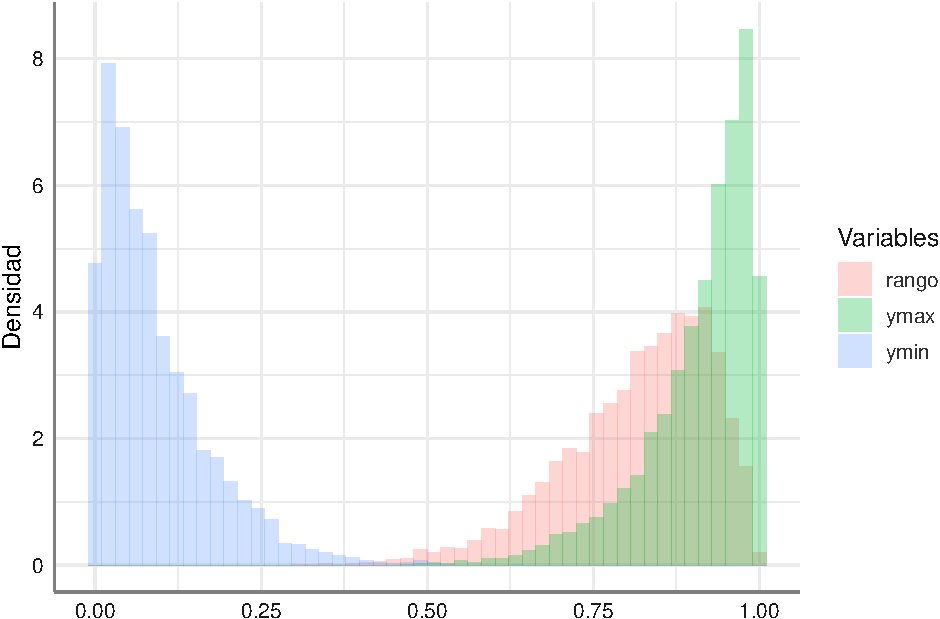
\includegraphics[width=0.95\linewidth]{01-Probabilidad_files/figure-latex/01-040-1} 

}

\caption{Simulaciones del mímimo, máximo y rango de X1,...,X10 v.a. U(9,1).}\label{fig:01-040}
\end{figure}

\begin{example}
\protect\hypertarget{exm:combined2}{}\label{exm:combined2}

En un estudio de calidad se está analizando el ajuste entre las pernos y las tuercas de cierto proceso de fabricación. Los pernos y las tuercas se fabrican de forma independiente y se colocan en dos cajas. Posteriormente se elige un perno y una tuerca y se prueba si encajan entre sí. Un perno y una tuerca ajustarán si el diámetro del agujero de la tuerca es mayor que el diámetro del perno y la diferencia entre estos diámetros no es mayor que 0.06 centímetros. Cuando no se cumplen estas especificaciones, tanto la tuerca como el perno se desechan. Las especificaciones de fabricación de los pernos indican que su diámetro se puede considerar que es una variable Normal con media 2 centimetros y desviación típica de 0.01 centímetros, mientras que el diámetro de las tuercas es una variable Normal con media 2.03 centímetros y desviación típica de 0.02 centímetros.

\begin{enumerate}
\def\labelenumi{\arabic{enumi}.}
\tightlist
\item
  ¿Cuál es la probabilidad de que encajen un perno y una tuerca elegidos al azar en una caja cualquiera?
\item
  Si se fabrican 10000 pernos y tuercas en un día, ¿cuántas desecharemos?
\item
  Si el porcentaje de desechos es inferior al 15\% en un día no se modificarán las especificaciones de fabricación ¿Consideras que deberían modificarse las especificaciones de fabricación?
\end{enumerate}

\end{example}

Partimos pues, para resolver el problema, de las variables \(T\sim N(2.03, 0.02)\), que representa el diámetro de una tuerca, y \(P \sim N(2, 0.01)\) que representa el diámetro de un perno. Las especificaciones de calidad exigen que \(T>P\) y que \(Dif=T-P\leq 0.6\), o lo que es lo mismo, \(0<Dif\leq 0.6\).

Veamos cómo podríamos simular para responder a las preguntas planteadas.

\begin{silverbox}

Algoritmo para obtener la diferencia entre los diámetros de las tuercas y los pernos.

\begin{itemize}
\tightlist
\item
  Paso 1. Fijar el número de simulaciones (\(nsim\)).
\end{itemize}

Repetir los pasos 2 a 4 hasta alacanzar el número de simulaciones fijado en el paso 1.

\begin{itemize}
\tightlist
\item
  Paso 2. Generar valores \(t_i\sim F(T)\) y \(p_i \sim F(P)\) de sus respectivas distribuciones.
\item
  Paso 3. Aplicando composición, calcular \(dif_i = t_i - p_i.\)
\item
  Paso 4. Verificar el requisito de calidad: \(0 < dif_i \leq 0.06\) y asignar \(valid_i = 1\) si se cumple con el criterio y \(valid_i = 0\) en otro caso.
\item
  Paso 5. Devolver el conjunto de valores simulados \(\{t_i, p_i, dif_i, valid_i\}_{i=1}^{nsim}.\)
\end{itemize}

\end{silverbox}

Pongamos en práctica el algoritmo diseñado.

\begin{Shaded}
\begin{Highlighting}[]
\CommentTok{\# Parámetros iniciales}
\NormalTok{nsim }\OtherTok{\textless{}{-}} \DecValTok{5000}
\FunctionTok{set.seed}\NormalTok{(}\DecValTok{12}\NormalTok{)}
\CommentTok{\# Generamos diámetros para tuercas y pernos}
\NormalTok{tuercas }\OtherTok{\textless{}{-}} \FunctionTok{rnorm}\NormalTok{(nsim, }\FloatTok{2.03}\NormalTok{, }\FloatTok{0.02}\NormalTok{)}
\NormalTok{pernos }\OtherTok{\textless{}{-}} \FunctionTok{rnorm}\NormalTok{(nsim, }\FloatTok{2.00}\NormalTok{, }\FloatTok{0.01}\NormalTok{)}
\CommentTok{\# Calculamos la diferencia y creamos filtro de calidad}
\NormalTok{diferencia }\OtherTok{\textless{}{-}}\NormalTok{ tuercas }\SpecialCharTok{{-}}\NormalTok{ pernos}
\NormalTok{valid}\OtherTok{\textless{}{-}} \DecValTok{1}\SpecialCharTok{*}\NormalTok{(diferencia }\SpecialCharTok{\textgreater{}}\DecValTok{0} \SpecialCharTok{\&}\NormalTok{ diferencia }\SpecialCharTok{\textless{}=} \FloatTok{0.06}\NormalTok{)}
\CommentTok{\# Devolvemos los valores }
\NormalTok{simulacion }\OtherTok{\textless{}{-}} \FunctionTok{data.frame}\NormalTok{(}\AttributeTok{sim =} \DecValTok{1}\SpecialCharTok{:}\NormalTok{nsim, }
                         \AttributeTok{tuercas =}\NormalTok{ tuercas, }
                         \AttributeTok{pernos =}\NormalTok{ pernos, }
                         \AttributeTok{diferencia=}\NormalTok{ diferencia, }
                         \AttributeTok{valid =}\NormalTok{ valid)}
\end{Highlighting}
\end{Shaded}

Representamos los datos simulados en la Figura \ref{fig:01-042}, con la que podemos ya responder la primera pregunta:

\begin{enumerate}
\def\labelenumi{\arabic{enumi}.}
\tightlist
\item
  ¿Cuál es la probabilidad de que encajen un perno y una tuerca elegidos al azar en una caja cualquiera? Como vemos en la gráfica superior izquierda, la respuesta es 0.82, a la vista de que el 82\% de las cajas inspeccionadas son válidas.
\end{enumerate}

\begin{Shaded}
\begin{Highlighting}[]
\CommentTok{\# Calidad del proceso}
\NormalTok{g1 }\OtherTok{\textless{}{-}}\NormalTok{ simulacion }\SpecialCharTok{\%\textgreater{}\%}
  \FunctionTok{count}\NormalTok{(valid)}\SpecialCharTok{\%\textgreater{}\%}
  \FunctionTok{mutate}\NormalTok{(}\AttributeTok{prop =} \FunctionTok{prop.table}\NormalTok{(n)) }\SpecialCharTok{\%\textgreater{}\%}
  \FunctionTok{ggplot}\NormalTok{(}\FunctionTok{aes}\NormalTok{(}\AttributeTok{x =} \FunctionTok{as.factor}\NormalTok{(valid), }\AttributeTok{y =}\NormalTok{ prop, }\AttributeTok{label =}\NormalTok{ scales}\SpecialCharTok{::}\FunctionTok{percent}\NormalTok{(prop))) }\SpecialCharTok{+} 
  \FunctionTok{geom\_col}\NormalTok{(}\AttributeTok{fill =} \StringTok{"steelblue"}\NormalTok{, }\AttributeTok{position =} \StringTok{"dodge"}\NormalTok{) }\SpecialCharTok{+}
  \FunctionTok{scale\_x\_discrete}\NormalTok{(}\AttributeTok{labels =} \FunctionTok{c}\NormalTok{(}\StringTok{"No"}\NormalTok{, }\StringTok{"Sí"}\NormalTok{)) }\SpecialCharTok{+}
  \FunctionTok{scale\_y\_continuous}\NormalTok{(}\AttributeTok{labels =}\NormalTok{ scales}\SpecialCharTok{::}\NormalTok{percent)}\SpecialCharTok{+}
  \FunctionTok{geom\_text}\NormalTok{(}\AttributeTok{position =} \FunctionTok{position\_dodge}\NormalTok{(}\AttributeTok{width =} \FloatTok{0.9}\NormalTok{), }\AttributeTok{vjust =} \FloatTok{1.5}\NormalTok{,}\AttributeTok{size =} \DecValTok{3}\NormalTok{)}\SpecialCharTok{+}
  \FunctionTok{labs}\NormalTok{(}\AttributeTok{x =} \StringTok{"Resultado del proceso: validez"}\NormalTok{, }\AttributeTok{y =} \StringTok{"Porcentaje"}\NormalTok{)}
\CommentTok{\# Diferencia}
\NormalTok{g2 }\OtherTok{\textless{}{-}} \FunctionTok{ggplot}\NormalTok{(simulacion, }\FunctionTok{aes}\NormalTok{(diferencia)) }\SpecialCharTok{+} 
  \FunctionTok{geom\_histogram}\NormalTok{(}\AttributeTok{fill =} \StringTok{"steelblue"}\NormalTok{,}\AttributeTok{color=}\StringTok{"grey"}\NormalTok{) }\SpecialCharTok{+}
  \FunctionTok{geom\_vline}\NormalTok{(}\AttributeTok{xintercept =} \FunctionTok{c}\NormalTok{(}\DecValTok{0}\NormalTok{, }\FloatTok{0.06}\NormalTok{), }\AttributeTok{col =} \StringTok{"red"}\NormalTok{) }\SpecialCharTok{+}
  \FunctionTok{labs}\NormalTok{(}\AttributeTok{x =} \StringTok{"Diferencia Tuerca{-}Perno"}\NormalTok{, }\AttributeTok{y =} \StringTok{"Frecuencia"}\NormalTok{)}
\CommentTok{\# Diámetros}
\NormalTok{orden }\OtherTok{\textless{}{-}} \FunctionTok{c}\NormalTok{(}\StringTok{"tuercas"}\NormalTok{, }\StringTok{"pernos"}\NormalTok{)}
\NormalTok{datos }\OtherTok{\textless{}{-}} \FunctionTok{pivot\_longer}\NormalTok{(simulacion, }\AttributeTok{cols =} \DecValTok{2}\SpecialCharTok{:}\DecValTok{3}\NormalTok{, }\AttributeTok{names\_to =} \StringTok{"Medida"}\NormalTok{, }\AttributeTok{values\_to =} \StringTok{"Valor"}\NormalTok{)}
\CommentTok{\# gráfico}
\NormalTok{g3 }\OtherTok{\textless{}{-}} \FunctionTok{ggplot}\NormalTok{(datos, }\FunctionTok{aes}\NormalTok{(Medida, Valor)) }\SpecialCharTok{+} 
  \FunctionTok{geom\_boxplot}\NormalTok{(}\AttributeTok{fill =} \StringTok{"steelblue"}\NormalTok{) }\SpecialCharTok{+}
  \FunctionTok{scale\_x\_discrete}\NormalTok{(}\AttributeTok{limits =}\NormalTok{ orden, }\AttributeTok{labels =}\NormalTok{ orden) }\SpecialCharTok{+}
  \FunctionTok{labs}\NormalTok{(}\AttributeTok{x =} \StringTok{""}\NormalTok{, }\AttributeTok{y =} \StringTok{"Diámetro"}\NormalTok{)}
\CommentTok{\# Combinación}
\FunctionTok{grid.arrange}\NormalTok{(g1, g2, g3, }\AttributeTok{nrow =} \DecValTok{2}\NormalTok{)}
\end{Highlighting}
\end{Shaded}

\begin{verbatim}
## `stat_bin()` using `bins = 30`. Pick better value with `binwidth`.
\end{verbatim}

\begin{figure}

{\centering 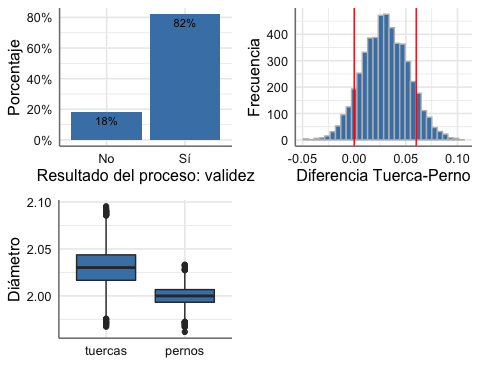
\includegraphics[width=0.95\linewidth]{01-Probabilidad_files/figure-latex/01-042-1} 

}

\caption{Simulaciones del proceso de calidad para tuercas y pernos.}\label{fig:01-042}
\end{figure}

Respondemos las siguientes preguntas:

\begin{enumerate}
\def\labelenumi{\arabic{enumi}.}
\setcounter{enumi}{1}
\tightlist
\item
  Si se fabrican 10000 pernos y tuercas en un día, ¿cuántas desecharemos? Si nuestra producción es de 10000 parejas, el número de parejas desechadas será igual a:
\end{enumerate}

\begin{Shaded}
\begin{Highlighting}[]
\DecValTok{10000}\SpecialCharTok{*}\NormalTok{(}\DecValTok{1} \SpecialCharTok{{-}} \FunctionTok{mean}\NormalTok{(simulacion}\SpecialCharTok{$}\NormalTok{valid }\SpecialCharTok{==} \DecValTok{1}\NormalTok{))}
\end{Highlighting}
\end{Shaded}

\begin{verbatim}
## [1] 1794
\end{verbatim}

\begin{enumerate}
\def\labelenumi{\arabic{enumi}.}
\setcounter{enumi}{2}
\tightlist
\item
  Si el porcentaje de desechos es inferior al 15\% en un día no se modificarán las especificaciones de fabricación ¿Consideras que deberían modificarse las especificaciones de fabricación? Realmente el porcentaje de piezas desechadas es del 18\% (gráfico superior izquierdo en la Figura \ref{fig:01-042}), por lo que la recomendación sería abordar un proceso de mejora en la fabricación para reducir los defectos.
\end{enumerate}

\begin{example}
\protect\hypertarget{exm:combined3}{}\label{exm:combined3}

Una empresa de fabricación de componentes para aviones tiene entre sus productos una barra que se coloca como sujeción en las alas, y que se construye mediante la unión consecutiva de tres secciones A, B, y C. Las especificaciones de fabricación establecen que la longitud (en pulgadas) de cada barra es una distribución Normal. Más concretamente la sección A tiene una media de 20 pulgadas y una varianza de 0.04. la longitud de la sección B tiene una media de 14 y varianza de 0.01, mientras que la sección C tiene una media de 26 y varianza 0.04. Las tres piezas se unen consecutivamente (A con B y B con C) de forma que se encajan superponiendo 2 pulgadas en cada unión. La barra sólo puede ser utilizada si su longitud total está entre 55.5 y 56.5 pulgadas.

\begin{enumerate}
\def\labelenumi{\arabic{enumi}.}
\tightlist
\item
  ¿Cuál es la probabilidad de que la barra sea utilizable?
\item
  Si en un mes se fabrican 25000 barras ¿cuál es el número de barras desechadas?
\item
  Por cada barra dentro de especificaciones se obtiene un beneficio de 300 euros, pero si se desecha, se genera una pérdida de 100 euros. ¿Cuál será el beneficio estimado en un mes?
\end{enumerate}

\end{example}

Si denominamos \(LA\), \(LB\), y \(LC\) a las variables aleatorias correspondientes a las longitudes de las secciones A, B, y C respectivamente, las distribuciones asociadas vienen dadas por:

\[LA \sim N(20, \sqrt{0.04}); \quad LB \sim N(14, \sqrt{0.01}); \quad  LC \sim N(26, \sqrt{0.04})\]

La otra variable involucrada es la suma de barra al unir las piezas, que se obtiene como \(L=LA+LB+LC-4\), dado que en cada junta se pierden 2 pulgadas. Las especificaciones de calidad sobre ella son \(55.5 \leq L \leq y 56.5\).

Proponemos pues, un algoritmo de simulación que nos permita simular la longitud total de la barra a partir de cada una de las secciones, y verificar si está dentro de las especificaciones de calidad establecidas.

\begin{silverbox}

\begin{itemize}
\tightlist
\item
  Paso 1. Fijar el número de simulaciones (\(nsim\)).
\end{itemize}

Repetir los pasos 2 a 4 hasta alcanzar el número de simulaciones fijado en el paso 1.

\begin{itemize}
\item
  Paso 2. Generar valores \(LA_i\), \(LB_i\), y \(LC_i\) a partir de sus distribuciones correspondientes.\\
\item
  Paso 3. Aplicando composición, calcular \(L_i = LA_i + LB_i + LC_i - 4.\)
\item
  Paso 4. Verificar el requisito de calidad: \(55.5 \leq L_i \leq 56.5\) y asignar \(valid_i = 1\) si lo cumple, y \(valid_i = 0\) si no lo cumple.
\item
  Paso 5. Devolver el conjunto de valores simulados \(\{LA_i, LB_i, LC_i, L_i, valid_i\}_{i=1}^{nsim}.\)
\end{itemize}

\end{silverbox}

Programemos el algoritmo.

\begin{Shaded}
\begin{Highlighting}[]
\CommentTok{\# Parámetros iniciales}
\NormalTok{nsim }\OtherTok{\textless{}{-}} \DecValTok{5000}
\FunctionTok{set.seed}\NormalTok{(}\DecValTok{12}\NormalTok{)}
\CommentTok{\# Generamos longitudes de las secciones}
\NormalTok{LA }\OtherTok{\textless{}{-}} \FunctionTok{rnorm}\NormalTok{(nsim, }\DecValTok{20}\NormalTok{, }\FunctionTok{sqrt}\NormalTok{(}\FloatTok{0.04}\NormalTok{))}
\NormalTok{LB }\OtherTok{\textless{}{-}} \FunctionTok{rnorm}\NormalTok{(nsim, }\DecValTok{14}\NormalTok{, }\FunctionTok{sqrt}\NormalTok{(}\FloatTok{0.01}\NormalTok{))}
\NormalTok{LC }\OtherTok{\textless{}{-}} \FunctionTok{rnorm}\NormalTok{(nsim, }\DecValTok{26}\NormalTok{, }\FunctionTok{sqrt}\NormalTok{(}\FloatTok{0.04}\NormalTok{))}
\CommentTok{\# Calculamos longitud total y verificamos requisitos}
\NormalTok{L }\OtherTok{\textless{}{-}}\NormalTok{ LA }\SpecialCharTok{+}\NormalTok{ LB }\SpecialCharTok{+}\NormalTok{ LC }\SpecialCharTok{{-}} \DecValTok{4}
\NormalTok{valid }\OtherTok{\textless{}{-}} \DecValTok{1}\SpecialCharTok{*}\NormalTok{(L }\SpecialCharTok{\textgreater{}=} \FloatTok{55.5} \SpecialCharTok{\&}\NormalTok{ L }\SpecialCharTok{\textless{}=} \FloatTok{56.5}\NormalTok{)}
\CommentTok{\# Devolvemos los valores }
\NormalTok{simulacion }\OtherTok{\textless{}{-}} \FunctionTok{data.frame}\NormalTok{(}\AttributeTok{sim =} \DecValTok{1}\SpecialCharTok{:}\NormalTok{nsim, }\AttributeTok{LA =}\NormalTok{ LA, }\AttributeTok{LB =}\NormalTok{ LB, }
                         \AttributeTok{LC =}\NormalTok{ LC, }\AttributeTok{L =}\NormalTok{ L,}\AttributeTok{valid=}\NormalTok{valid)}
\end{Highlighting}
\end{Shaded}

Respondamos a las preguntas a partir de las simulaciones obtenidas.

\begin{enumerate}
\def\labelenumi{\arabic{enumi}.}
\tightlist
\item
  ¿Cuál es la probabilidad de que la barra sea utilizable? La respuesta viene aproximada por la proporción de piezas válidas. Calculamos también un intervalo de confianza utilizando la ecuación \eqref{eq:icMC}.
\end{enumerate}

\begin{Shaded}
\begin{Highlighting}[]
\CommentTok{\#  Pr proceso cumpla criterios calidad}
\NormalTok{p }\OtherTok{=} \FunctionTok{mean}\NormalTok{(simulacion}\SpecialCharTok{$}\NormalTok{valid }\SpecialCharTok{==} \DecValTok{1}\NormalTok{)}
\NormalTok{error }\OtherTok{=} \FunctionTok{sqrt}\NormalTok{((}\FunctionTok{sum}\NormalTok{(simulacion}\SpecialCharTok{$}\NormalTok{valid}\SpecialCharTok{{-}}\NormalTok{p)}\SpecialCharTok{\^{}}\DecValTok{2}\NormalTok{)}\SpecialCharTok{/}\NormalTok{(nsim}\SpecialCharTok{\^{}}\DecValTok{2}\NormalTok{))}
\NormalTok{alpha }\OtherTok{=} \FloatTok{0.05} \CommentTok{\# 1{-}alpha=nivel de confianza para el IC}
\NormalTok{ic.low }\OtherTok{=}\NormalTok{ p }\SpecialCharTok{{-}} \FunctionTok{qnorm}\NormalTok{(}\DecValTok{1}\SpecialCharTok{{-}}\NormalTok{alpha}\SpecialCharTok{/}\DecValTok{2}\NormalTok{)}\SpecialCharTok{*}\NormalTok{error}
\NormalTok{ic.up }\OtherTok{=}\NormalTok{ p }\SpecialCharTok{+} \FunctionTok{qnorm}\NormalTok{(}\DecValTok{1}\SpecialCharTok{{-}}\NormalTok{alpha}\SpecialCharTok{/}\DecValTok{2}\NormalTok{)}\SpecialCharTok{*}\NormalTok{error}
\FunctionTok{cat}\NormalTok{(}\StringTok{"Pr(barra utilizable)="}\NormalTok{, p)}
\end{Highlighting}
\end{Shaded}

\begin{verbatim}
## Pr(barra utilizable)= 0.9016
\end{verbatim}

\begin{Shaded}
\begin{Highlighting}[]
\FunctionTok{cat}\NormalTok{(}\StringTok{"Error de la aproximación="}\NormalTok{, error)}
\end{Highlighting}
\end{Shaded}

\begin{verbatim}
## Error de la aproximación= 4.298784e-17
\end{verbatim}

\begin{Shaded}
\begin{Highlighting}[]
\FunctionTok{cat}\NormalTok{(}\StringTok{"IC("}\NormalTok{, }\DecValTok{1}\SpecialCharTok{{-}}\NormalTok{alpha,}\StringTok{"\%)= ["}\NormalTok{, ic.low,}\StringTok{","}\NormalTok{, ic.up,}\StringTok{"]"}\NormalTok{)}
\end{Highlighting}
\end{Shaded}

\begin{verbatim}
## IC( 0.95 %)= [ 0.9016 , 0.9016 ]
\end{verbatim}

Dado el error tan pequeño que genera el proceso de simulación, la estimación proporcionada es claramente precisa.

\begin{enumerate}
\def\labelenumi{\arabic{enumi}.}
\setcounter{enumi}{1}
\tightlist
\item
  Si en un mes se fabrican 25000 barras ¿cuál es el número de barras desechadas?
\end{enumerate}

\begin{Shaded}
\begin{Highlighting}[]
\NormalTok{desechos}\OtherTok{=}\DecValTok{25000}\SpecialCharTok{*}\NormalTok{(}\DecValTok{1}\SpecialCharTok{{-}}\NormalTok{p)}
\FunctionTok{cat}\NormalTok{(}\StringTok{"Barras desechadas en un mes:"}\NormalTok{, desechos)}
\end{Highlighting}
\end{Shaded}

\begin{verbatim}
## Barras desechadas en un mes: 2460
\end{verbatim}

\begin{enumerate}
\def\labelenumi{\arabic{enumi}.}
\setcounter{enumi}{2}
\tightlist
\item
  Por cada barra dentro de especificaciones se obtiene un beneficio de 300 euros, pero si se desecha, se genera una pérdida de 100 euros. ¿Cuál será el beneficio estimado en un mes?
\end{enumerate}

\begin{Shaded}
\begin{Highlighting}[]
\NormalTok{benef}\OtherTok{=}\NormalTok{(}\DecValTok{25000}\SpecialCharTok{{-}}\NormalTok{desechos)}\SpecialCharTok{*}\DecValTok{300}\SpecialCharTok{{-}}\NormalTok{desechos}\SpecialCharTok{*}\DecValTok{100}
\FunctionTok{cat}\NormalTok{(}\StringTok{"Beneficio obtenido en un mes:"}\NormalTok{, benef, }\StringTok{"€"}\NormalTok{)}
\end{Highlighting}
\end{Shaded}

\begin{verbatim}
## Beneficio obtenido en un mes: 6516000 €
\end{verbatim}

\hypertarget{modelos-secuenciales}{%
\subsection{Modelos secuenciales}\label{modelos-secuenciales}}

En la última sección para variables de tipo continuo presentamos los primeros modelos de simulación para variables aleatorias que actúan de forma consecutiva a lo largo del tiempo. Será pues, una introducción a los modelos estocásticos que estudiaremos en el resto de unidades. En estas situaciones todas las variables involucradas en el sistema hacen referencia al tiempo de ocurrencia de los eventos de interés. Trabajemos con ejemplos, para entender los conceptos y problemas involucrados.

\begin{example}
\protect\hypertarget{exm:secuencia1}{}\label{exm:secuencia1}

El equipo de mantenimiento de una empresa debe programar las visitas a cierta instalación para establecer una calendario eficiente de revisiones. El sistema que debe analizar está compuesto por tres procesos (A, B, y C) que funcionan de forma independiente, pero que están conectados en serie, de forma que todo el sistema se detiene si un proceso falla. El tiempo de vida o tiempo hasta un fallo o avería, medido en horas, para cada uno de los procesos se puede considerar aleatorio y responde a distribuciones exponenciales con medias 1000, 333, y 167 respectivamente.

El proceso de fabricación completo, que involucra a los tres procesos A, B y C, funciona 24 horas al día y completa un ciclo cada siete días, tras el cual realiza un parón para tareas de mantenimiento. En ese ciclo, los procesos A, B y C operan consecutivamente durante un día: \(A\) trabaja durante 15.6 horas, luego entra en funcionamiento el proceso \(B\) durante 5.52 horas, y finalmente el \(C\) durante 2.88 horas.

En la actualidad el equipo de manteniento está interesado en reajustar el ciclo para realizar las labores de mantenimiento, si fuera necesario, y reducir el tiempo muerto en que el sistema está parado, pues en estos momentos se dedican 24 horas tras cada ciclo, para las tareas de mantenimiento.

\begin{enumerate}
\def\labelenumi{\arabic{enumi}.}
\tightlist
\item
  ¿Cuál es la probabilidad de que el sistema falle antes de finalizar un ciclo de trabajo?
\item
  ¿Cuál de los procesos está generando más parones en el ciclo debidos a una avería?
\item
  ¿Cuál es el tiempo medio de funcionamiento del sistema sin ningún fallo? Interesa además, un rango o intervalo de confianza para dicha estimación. ¿Cuál sería el tiempo óptimo del ciclo para abordar las tareas de mantenimiento?
\end{enumerate}

\end{example}

En primer lugar modelicemos el sistema en base a la información proporcionada. Definamos las variables aleatorias \(TA\), \(TB\), y \(TC\) que representan, respectivamente, el tiempo de funcionamiento -o tiempo a fallo- (en horas) de cada proceso A, B y C. Sus distribuciones son: \[TA \sim Exp(1/1000); \quad TB \sim Exp(1/333); \quad TC \sim Exp(1/167).\] También son importantes las siguientes cantidades: - El tiempo de funcionamiento requerido cada día para cada uno de los procesos \(ta=15.6, tb=5.52, tc=2.88\) y el número de días que conforma cada ciclo, \(nciclo=7\).

\begin{itemize}
\tightlist
\item
  El tiempo de vida potencial del sistema completo, esto es, el tiempo \(T\) que funciona el sistema de fabricación hasta un fallo, y que se calcula a partir del mínimo número de días que funciona cada proceso, \(min \{TA/ta,TB/tb,TC/tb\}\).
\end{itemize}

Propongamos pues, un algoritmo de simulación que reproduzca el proceso de fabricación para un número \(nsim\) de ciclos simulados, cuyas simulaciones permitan responder a las preguntas planteadas.

\begin{silverbox}

\textbf{Algoritmo para el estudio de fallo del sistema}

\begin{itemize}
\tightlist
\item
  Paso 1. Fijar el número de simulaciones o ciclos a simular (\(nsim\)).
\end{itemize}

Repetir los pasos 2 a 4 tantas veces como simulaciones a generar (\emph{nsim}).

\begin{itemize}
\item
  Paso 2. Generar valores \(TA_i\), \(TB_i\), y \(TC_i\) de los tiempos a fallo de cada proceso según su distribución.
\item
  Paso 3. Calcular el número de días que dura sin fallos cada proceso, con los ratios \(rt_i=\{TA_i/ta, TB_i/tb, TC_i/tc\}\). Identificar cuál falla primero (\(min(rt_i)\)).
\item
  Paso 4. Verificar si el primero en fallar lo hace antes de terminar el ciclo, \(min(rt_i)<=7\). Si es que sí, guardar cuál es el proceso responsable del fallo y calcular la duración del ciclo mediante \(24*rt_i\) horas. Si es que no, indicarlo y especificar como duración del ciclo \(24*7\) horas.
\item
  Paso 5. Devolver los valores de las simulaciones de los tiempos a fallo de cada proceso, de la duración del ciclo, el indicador de fallo y el proceso responsable en cada ciclo (simulación).
\end{itemize}

\end{silverbox}

\begin{Shaded}
\begin{Highlighting}[]
\CommentTok{\# Función para simular el proceso de fabricación con tres subprocesos ABC encadenados.}
\NormalTok{simula.proceso}\OtherTok{=}\ControlFlowTok{function}\NormalTok{(nsim, nciclo, alpha, beta, delta, ta, tb, tc)\{}
\CommentTok{\# semilla=Semilla aleatoria y nsim=nº simulaciones o ciclos a simular}
\CommentTok{\#nciclo es el número de días del ciclo}
\CommentTok{\# alpha, beta y delta son los parámetros de las exponenciales TA,TB,TC}
\CommentTok{\# ta,tb y tc son los tiempos de funcionamiento diarios para los procesos A, B y C.}
\NormalTok{Tciclo}\OtherTok{=}\NormalTok{Dciclo }\OtherTok{=} \FunctionTok{rep}\NormalTok{(}\DecValTok{0}\NormalTok{, nsim)   }\CommentTok{\# tiempo de ciclo (en horas T y días D)}
\NormalTok{Tpotencial }\OtherTok{=} \FunctionTok{rep}\NormalTok{(}\DecValTok{0}\NormalTok{, nsim)      }\CommentTok{\# tiempo(en horas) que funcionaría sin fallos}
\NormalTok{fallo }\OtherTok{=} \FunctionTok{c}\NormalTok{()                   }\CommentTok{\# qué proceso ha fallado en cada ciclo}
\NormalTok{procesos }\OtherTok{=} \FunctionTok{c}\NormalTok{(}\StringTok{"A"}\NormalTok{, }\StringTok{"B"}\NormalTok{, }\StringTok{"C"}\NormalTok{)}

\CommentTok{\# simulamos las duraciones para todos los ciclos}
\NormalTok{TA }\OtherTok{=} \FunctionTok{rexp}\NormalTok{(nsim, alpha)  }
\NormalTok{TB }\OtherTok{=} \FunctionTok{rexp}\NormalTok{(nsim, beta)}
\NormalTok{TC }\OtherTok{=} \FunctionTok{rexp}\NormalTok{(nsim, delta)}
\NormalTok{t }\OtherTok{=} \FunctionTok{c}\NormalTok{(ta, tb, tc) }\CommentTok{\# funcionamiento diario de cada proceso}

\ControlFlowTok{for}\NormalTok{(j }\ControlFlowTok{in} \DecValTok{1}\SpecialCharTok{:}\NormalTok{nsim)\{}
\NormalTok{  T }\OtherTok{=} \FunctionTok{c}\NormalTok{(TA[j], TB[j], TC[j])      }\CommentTok{\# tiempos de vida para el ciclo j}
\NormalTok{  nfallo }\OtherTok{=}\NormalTok{ T}\SpecialCharTok{/}\NormalTok{t                  }\CommentTok{\# número días que funcionará cada proceso}
\NormalTok{  falla }\OtherTok{=} \FunctionTok{which.min}\NormalTok{(nfallo)     }\CommentTok{\# qué proceso falla primero}
  \ControlFlowTok{if}\NormalTok{(nfallo[falla] }\SpecialCharTok{\textless{}=}\NormalTok{ nciclo)\{  }\CommentTok{\# si falla antes de cerrar el ciclo}
\NormalTok{   fallo[j] }\OtherTok{=}\NormalTok{ procesos[falla]   }\CommentTok{\#identificamos el proceso que falla}
\NormalTok{   Dciclo[j] }\OtherTok{=}\NormalTok{ T[falla]}\SpecialCharTok{/}\NormalTok{t[falla]   }\CommentTok{\# y lo pasamos a días}
\NormalTok{   Tciclo[j] }\OtherTok{=}\NormalTok{ Tpotencial[j]}\OtherTok{=}\DecValTok{24}\SpecialCharTok{*}\NormalTok{Dciclo[j]   }\CommentTok{\# duración del ciclo (en horas)}
\NormalTok{  \}}
  \ControlFlowTok{else}\NormalTok{\{                       }\CommentTok{\#si no falla ninguno antes de cerrar el ciclo}
\NormalTok{    Tciclo[j] }\OtherTok{=} \DecValTok{24}\SpecialCharTok{*}\DecValTok{7}            \CommentTok{\#cerramos el ciclo sin fallos}
\NormalTok{    Dciclo[j] }\OtherTok{=} \DecValTok{7}
\NormalTok{    fallo[j] }\OtherTok{=} \StringTok{"No"}
\NormalTok{    Tpotencial[j] }\OtherTok{=}\NormalTok{ T[falla]}\SpecialCharTok{/}\NormalTok{t[falla]}\SpecialCharTok{*}\DecValTok{24}    \CommentTok{\# y guardamos la duración potencial }
\NormalTok{  \}}
\NormalTok{\} }\CommentTok{\# fin del for (j)}
\NormalTok{resultado }\OtherTok{=} \FunctionTok{data.frame}\NormalTok{(}\AttributeTok{ciclo =} \DecValTok{1}\SpecialCharTok{:}\NormalTok{nsim, fallo,}
                     \AttributeTok{Tciclo =} \FunctionTok{round}\NormalTok{(Tciclo, }\DecValTok{2}\NormalTok{),}\AttributeTok{Dciclo =} \FunctionTok{round}\NormalTok{(Dciclo, }\DecValTok{2}\NormalTok{),}
                     \AttributeTok{Tpotencial =} \FunctionTok{round}\NormalTok{(Tpotencial, }\DecValTok{2}\NormalTok{),}
                     \AttributeTok{DA =} \FunctionTok{round}\NormalTok{(TA}\SpecialCharTok{/}\NormalTok{ta, }\DecValTok{2}\NormalTok{), }\AttributeTok{DB =} \FunctionTok{round}\NormalTok{(TB}\SpecialCharTok{/}\NormalTok{tb, }\DecValTok{2}\NormalTok{), }\AttributeTok{DC =} \FunctionTok{round}\NormalTok{(TC}\SpecialCharTok{/}\NormalTok{tc, }\DecValTok{2}\NormalTok{))}

\FunctionTok{return}\NormalTok{(resultado)}
\NormalTok{\}}
\end{Highlighting}
\end{Shaded}

Lanzamos el proceso para los valores del ejemplo, y visualizamos los resultados en la Tabla \ref{tab:procesofabricacion}

\begin{Shaded}
\begin{Highlighting}[]
\NormalTok{nciclo }\OtherTok{=} \DecValTok{7}\NormalTok{; alpha }\OtherTok{=} \DecValTok{1}\SpecialCharTok{/}\DecValTok{1000}\NormalTok{; beta }\OtherTok{=} \DecValTok{1}\SpecialCharTok{/}\DecValTok{333}\NormalTok{; delta }\OtherTok{=} \DecValTok{1}\SpecialCharTok{/}\DecValTok{167}
\NormalTok{ta }\OtherTok{=} \FloatTok{15.6}\NormalTok{;tb }\OtherTok{=} \FloatTok{5.52}\NormalTok{; tc }\OtherTok{=} \FloatTok{2.88}
\NormalTok{semilla }\OtherTok{=} \DecValTok{12}

\FunctionTok{set.seed}\NormalTok{(semilla)}
\NormalTok{nsim}\OtherTok{=}\DecValTok{5000}                  
\NormalTok{simulacion}\OtherTok{=}\FunctionTok{simula.proceso}\NormalTok{(nsim,nciclo,alpha,beta,delta,ta,tb,tc)}
\FunctionTok{kbl}\NormalTok{(}\FunctionTok{head}\NormalTok{(simulacion),}\AttributeTok{caption=}\StringTok{"Simulaciones para el proceso de fabricación con tres subprocesos encadenados A, B y C. Tipo de fallo, tiempos de funcionamiento del sistema (Tciclo en horas, Dciclo en días) y tiempo de funcionamiento potencial (Tpotencial en horas). Días de vida DA, DB, DC de los procesos."}\NormalTok{) }\SpecialCharTok{\%\textgreater{}\%}
 \FunctionTok{kable\_styling}\NormalTok{(}\AttributeTok{bootstrap\_options =} \StringTok{"striped"}\NormalTok{, }\AttributeTok{full\_width =}\NormalTok{ F, }\AttributeTok{position =} \StringTok{"left"}\NormalTok{)}
\end{Highlighting}
\end{Shaded}

\begin{table}

\caption{\label{tab:procesofabricacion}Simulaciones para el proceso de fabricación con tres subprocesos encadenados A, B y C. Tipo de fallo, tiempos de funcionamiento del sistema (Tciclo en horas, Dciclo en días) y tiempo de funcionamiento potencial (Tpotencial en horas). Días de vida DA, DB, DC de los procesos.}
\begin{tabular}[t]{r|l|r|r|r|r|r|r}
\hline
ciclo & fallo & Tciclo & Dciclo & Tpotencial & DA & DB & DC\\
\hline
1 & No & 168.00 & 7.00 & 219.46 & 140.33 & 9.14 & 59.78\\
\hline
2 & No & 168.00 & 7.00 & 171.59 & 40.74 & 7.15 & 18.27\\
\hline
3 & C & 96.63 & 4.03 & 96.63 & 7.52 & 32.32 & 4.03\\
\hline
4 & B & 34.45 & 1.44 & 34.45 & 183.16 & 1.44 & 259.42\\
\hline
5 & No & 168.00 & 7.00 & 617.69 & 116.45 & 87.16 & 25.74\\
\hline
6 & No & 168.00 & 7.00 & 435.89 & 18.16 & 83.25 & 112.44\\
\hline
\end{tabular}
\end{table}

\begin{enumerate}
\def\labelenumi{\arabic{enumi}.}
\tightlist
\item
  ¿Cuál es la probabilidad de que el sistema falle antes de finalizar un ciclo de trabajo?
\end{enumerate}

\begin{Shaded}
\begin{Highlighting}[]
\NormalTok{m }\OtherTok{=} \FunctionTok{mean}\NormalTok{(simulacion}\SpecialCharTok{$}\NormalTok{fallo }\SpecialCharTok{!=} \StringTok{"No"}\NormalTok{)}
\NormalTok{error }\OtherTok{=} \FunctionTok{sqrt}\NormalTok{(}\FunctionTok{sum}\NormalTok{(((simulacion}\SpecialCharTok{$}\NormalTok{fallo }\SpecialCharTok{!=} \StringTok{"No"}\NormalTok{)}\SpecialCharTok{*}\DecValTok{1}\SpecialCharTok{{-}}\NormalTok{m)}\SpecialCharTok{\^{}}\DecValTok{2}\NormalTok{) }\SpecialCharTok{/}\NormalTok{ (nsim}\SpecialCharTok{\^{}}\DecValTok{2}\NormalTok{))}
\NormalTok{ic.low }\OtherTok{=}\NormalTok{ m }\SpecialCharTok{{-}} \FunctionTok{qnorm}\NormalTok{(}\FloatTok{0.975}\NormalTok{)}\SpecialCharTok{*}\NormalTok{error}
\NormalTok{ic.up }\OtherTok{=}\NormalTok{ m }\SpecialCharTok{+} \FunctionTok{qnorm}\NormalTok{(}\FloatTok{0.975}\NormalTok{)}\SpecialCharTok{*}\NormalTok{error}
\FunctionTok{cat}\NormalTok{(}\StringTok{"Pr(fallo antes del ciclo="}\NormalTok{,m)}
\end{Highlighting}
\end{Shaded}

\begin{verbatim}
## Pr(fallo antes del ciclo= 0.2876
\end{verbatim}

\begin{Shaded}
\begin{Highlighting}[]
\FunctionTok{cat}\NormalTok{(}\StringTok{"IC(Probabilidad)=["}\NormalTok{,}\FunctionTok{round}\NormalTok{(ic.low, }\DecValTok{4}\NormalTok{),}\StringTok{","}\NormalTok{,}\FunctionTok{round}\NormalTok{(ic.up, }\DecValTok{4}\NormalTok{),}\StringTok{"]"}\NormalTok{)}
\end{Highlighting}
\end{Shaded}

\begin{verbatim}
## IC(Probabilidad)=[ 0.2751 , 0.3001 ]
\end{verbatim}

\begin{enumerate}
\def\labelenumi{\arabic{enumi}.}
\setcounter{enumi}{1}
\tightlist
\item
  ¿Cuál de los procesos está generando más parones en el ciclo debidos a una avería?
\end{enumerate}

En la Figura \ref{fig:01-048} representamos (a la izquierda) el porcentaje que se detiene el proceso de fabricación antes de finalizar el ciclo, para cada uno de los tipos de fallo posible (debido a un parón en A, B o C), y difieren muy poco entre sí. El más frecuente, dentro de la similaridad es el fallo en el proceso C, con una probabilidad de 0.0986. A la derecha de la gráfica vemos cómo los tres tipos de fallo están dando tiempos de fabricación muy similares en media y variabilidad.

\begin{Shaded}
\begin{Highlighting}[]
\CommentTok{\#  Representación gráfica del ciclo de vida: tabla de probabilidades}
\NormalTok{g1 }\OtherTok{=}\NormalTok{ simulacion }\SpecialCharTok{\%\textgreater{}\%}
  \FunctionTok{group\_by}\NormalTok{(fallo) }\SpecialCharTok{\%\textgreater{}\%}
  \FunctionTok{summarise}\NormalTok{(}\AttributeTok{n =} \FunctionTok{n}\NormalTok{(), }\AttributeTok{prop =}\NormalTok{ n}\SpecialCharTok{/}\FunctionTok{nrow}\NormalTok{(simulacion)) }\SpecialCharTok{\%\textgreater{}\%}
  \FunctionTok{ggplot}\NormalTok{(}\FunctionTok{aes}\NormalTok{(}\AttributeTok{x =}\NormalTok{ fallo, }\AttributeTok{y =}\NormalTok{ prop)) }\SpecialCharTok{+}
    \FunctionTok{geom\_col}\NormalTok{(}\FunctionTok{aes}\NormalTok{(}\AttributeTok{fill =}\NormalTok{ fallo), }\AttributeTok{position =} \StringTok{"dodge"}\NormalTok{) }\SpecialCharTok{+}
    \FunctionTok{geom\_text}\NormalTok{(}\FunctionTok{aes}\NormalTok{(}\AttributeTok{label =}\NormalTok{ scales}\SpecialCharTok{::}\FunctionTok{percent}\NormalTok{(prop), }
                  \AttributeTok{y =}\NormalTok{ prop, }\AttributeTok{group =}\NormalTok{ fallo),}
              \AttributeTok{position =} \FunctionTok{position\_dodge}\NormalTok{(}\AttributeTok{width =} \FloatTok{0.9}\NormalTok{),}
              \AttributeTok{vjust =} \FloatTok{1.5}\NormalTok{)}\SpecialCharTok{+}
  \FunctionTok{labs}\NormalTok{(}\AttributeTok{x =} \StringTok{"Tipo de fallo"}\NormalTok{,}\AttributeTok{y =} \StringTok{"Proporción"}\NormalTok{)}\SpecialCharTok{+}
  \FunctionTok{theme}\NormalTok{(}\AttributeTok{legend.position =} \StringTok{"none"}\NormalTok{)}


\CommentTok{\# Tiempo de vida en función del ciclo}
\NormalTok{g2 }\OtherTok{\textless{}{-}} \FunctionTok{ggplot}\NormalTok{(simulacion, }\FunctionTok{aes}\NormalTok{(fallo, Tciclo)) }\SpecialCharTok{+} 
  \FunctionTok{geom\_boxplot}\NormalTok{(}\AttributeTok{fill =} \StringTok{"steelblue"}\NormalTok{) }\SpecialCharTok{+}
  \FunctionTok{labs}\NormalTok{(}\AttributeTok{x =} \StringTok{"Tipo de fallo"}\NormalTok{, }\AttributeTok{y =} \StringTok{"Tiempo de funcionamiento (horas)"}\NormalTok{)}
\FunctionTok{grid.arrange}\NormalTok{(g1, g2, }\AttributeTok{nrow =} \DecValTok{1}\NormalTok{)}
\end{Highlighting}
\end{Shaded}

\begin{figure}

{\centering 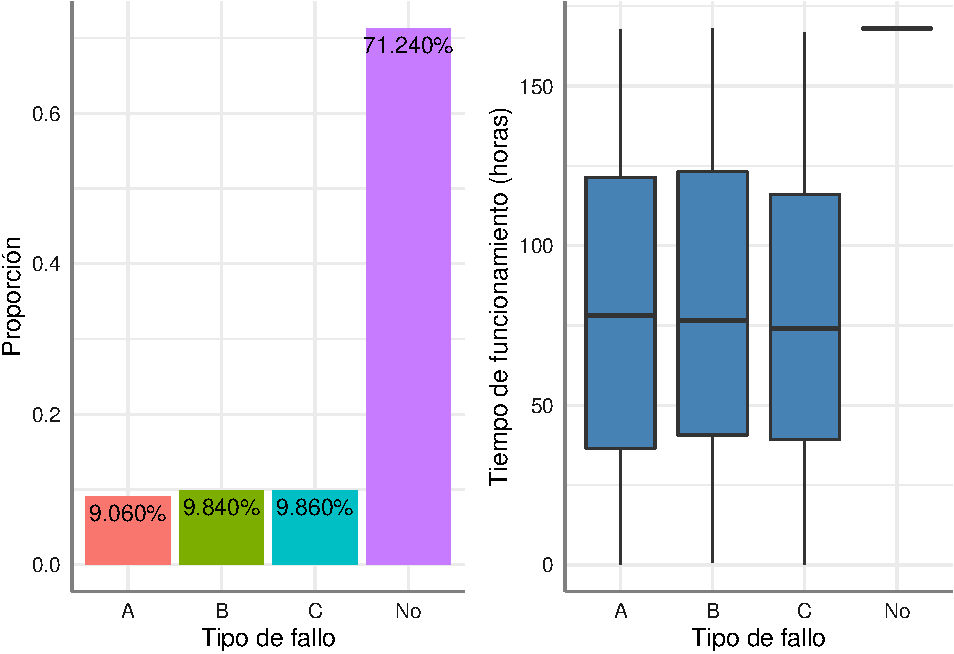
\includegraphics[width=0.95\linewidth]{01-Probabilidad_files/figure-latex/01-048-1} 

}

\caption{Gráfico del ciclo de vida y de la probabilidad del tiempo de fabricación sin fallos.}\label{fig:01-048}
\end{figure}

\begin{enumerate}
\def\labelenumi{\arabic{enumi}.}
\setcounter{enumi}{2}
\tightlist
\item
  ¿Cuál es el tiempo medio de funcionamiento del sistema sin ningún fallo? Interesa además, un rango o intervalo de confianza para dicha estimación. ¿Cuál sería el tiempo óptimo del ciclo para abordar las tareas de mantenimiento?
\end{enumerate}

Respondemos esta pregunta utilizando no el tiempo de ciclo impuesto como cota superior, sino el tiempo de funcionamiento que el sistema es capaz de aguantar sin fallos, recogido en la variable \texttt{Tpotencial}(en horas). Damos una estimación y construimos un intervalo de confianza al 95\% para responder la pregunta.

\begin{Shaded}
\begin{Highlighting}[]
\NormalTok{m }\OtherTok{=} \FunctionTok{mean}\NormalTok{(simulacion}\SpecialCharTok{$}\NormalTok{Tpotencial)}
\NormalTok{error }\OtherTok{=} \FunctionTok{sqrt}\NormalTok{(}\FunctionTok{sum}\NormalTok{((simulacion}\SpecialCharTok{$}\NormalTok{Tpotencial}\SpecialCharTok{{-}}\NormalTok{m)}\SpecialCharTok{\^{}}\DecValTok{2}\NormalTok{) }\SpecialCharTok{/}\NormalTok{ (nsim}\SpecialCharTok{\^{}}\DecValTok{2}\NormalTok{))}
\NormalTok{ic.low }\OtherTok{=}\NormalTok{ m }\SpecialCharTok{{-}} \FunctionTok{qnorm}\NormalTok{(}\FloatTok{0.975}\NormalTok{)}\SpecialCharTok{*}\NormalTok{error}
\NormalTok{ic.up }\OtherTok{=}\NormalTok{ m }\SpecialCharTok{+} \FunctionTok{qnorm}\NormalTok{(}\FloatTok{0.975}\NormalTok{)}\SpecialCharTok{*}\NormalTok{error}
\FunctionTok{cat}\NormalTok{(}\StringTok{"E(Tpotencial)="}\NormalTok{,}\FunctionTok{round}\NormalTok{(m}\SpecialCharTok{/}\DecValTok{24}\NormalTok{, }\DecValTok{2}\NormalTok{))}
\end{Highlighting}
\end{Shaded}

\begin{verbatim}
## E(Tpotencial)= 20.54
\end{verbatim}

\begin{Shaded}
\begin{Highlighting}[]
\FunctionTok{cat}\NormalTok{(}\StringTok{"IC(estimación)=["}\NormalTok{,}\FunctionTok{round}\NormalTok{(ic.low}\SpecialCharTok{/}\DecValTok{24}\NormalTok{, }\DecValTok{2}\NormalTok{),}\StringTok{","}\NormalTok{,}\FunctionTok{round}\NormalTok{(ic.up}\SpecialCharTok{/}\DecValTok{24}\NormalTok{, }\DecValTok{2}\NormalTok{),}\StringTok{"]"}\NormalTok{)}
\end{Highlighting}
\end{Shaded}

\begin{verbatim}
## IC(estimación)=[ 19.98 , 21.11 ]
\end{verbatim}

Resulta pues, que el sistema de fabricación tiene capacidad para funcionar sin fallos una media de 20.5 días, y el intervalo de confianza da un límite inferior de 19.98, lo que da justificaría, con unas garantías del 97.5\%, reajustar el ciclo y darle un tamaño de 20 días, reduciendo así considerablemente los parones de un día completo de mantenimiento cada 7 en funcionamiento.

\begin{example}
\protect\hypertarget{exm:secuencia2}{}\label{exm:secuencia2}El gerente de una empresa que se dedica a la extracción y venta de piedra natural está preocupado porque piensa que hay un problema con la máquina que se dedica a cortar, en bloques más manejables, los bloques de piedra que vienen desde la cantera. La máquina trabaja durante 24 horas al día los 365 días del año, y las especificaciones de calidad establecen que la media y varianza del tiempo hasta que la máquina se detiene por un fallo, \(TF\), han de ser de 80 y 50 horas respectivamente.

En el histórico de mantenimiento de la empresa se han detectado tres tipos de fallos que se han catalogado como leves, moderados y graves. Además, la información del equipo de mantenimiento indica que el tipo de fallo que se produce está muy relacionado con el tiempo de funcionamiento de la máquina, de forma que la probabilidad de que se produzca un fallo u otro varía de acuerdo a la tabla siguiente:

\begin{longtable}[]{@{}llll@{}}
\toprule
TF vs Fallo & Leve & Moderado & Grave \\
\midrule
\endhead
\(TF \leq 1500\) & 0.85 & 0.10 & 0.05 \\
\(1500 < TF \leq 3000\) & 0.75 & 0.15 & 0.10 \\
\(TF > 3000\) & 0.65 & 0.20 & 0.15 \\
\bottomrule
\end{longtable}

Los tiempos de reparación (medidos en minutos), \(TR\), tienen medias y varianzas dadas por:

\begin{longtable}[]{@{}lll@{}}
\toprule
Fallo & Media & Varianza \\
\midrule
\endhead
Leve & 30 & 15 \\
Moderado & 60 & 30 \\
Grave & 120 & 45 \\
\bottomrule
\end{longtable}

Además se sabe que si el fallo es leve, no es necesario detener la producción por completo, ya que esta se puede reducir al 60\% y seguir trabajando mientras se realiza la reparación. En los otros dos casos la máquina debe detenerse por completo.

El gerente está interesado en conocer el funcionamiento de la máquina en los próximos seis meses asumiendo que las variables de tiempo de funcionamiento y tiempo de reparación son de tipo Weibull. En concreto desea saber qué porcentaje del tiempo la máquina estará trabajando a pleno rendimiento, a rendimiento reducido y parada.
\end{example}

Antes de plantear un algoritmo de simulación, tratemos de entender y modelizar bien la secuenciación de variables involucradas, según las especificaciones dadas. Las variables descritas son:

\begin{itemize}
\tightlist
\item
  \(TF\): Tiempo de funcionamiento de la máquina hasta fallo.
\item
  \(averia\): Tipo de avería cuando el sistema falla: leve, moderado, grave. Su distribución depende de \(tf\).
\item
  \(TR.xx\): Tiempo de reparación para una avería ``xx=\{leve, moderado, grave\}'', que depende del tipo de avería.
\end{itemize}

El tiempo de funcionamiento a pleno rendimiento vendrá dado por el tiempo acumulado en el que el sistema funciona sin ningún fallo, obtenido de todos los \(TF\) simulados. El funcionamiento a rendimiento reducido se dará mientras se está reparando alguna avería de tipo leve. El tiempo de parada del sistema corresponde a los periodos en los que se está reparando alguna avería de tipo moderada o grave. Puesto que el funcionamiento del sistema depende del tipo de avería, nos interesará guardar información sobre el tipo de avería que se está reparando, información que recopilaremos en la variable \(averia\). El tiempo dedicado a reparaciones lo guardaremos en una variable global denominada \(TREPARA\), que nos permitirá calcular cuándo el sistema no funciona a pleno rendimiento.

\begin{itemize}
\tightlist
\item
  \(TREPARA\): Tiempo total dedicado a reparaciones.
\end{itemize}

En cada simulación nos interesará contabilizar el tiempo transcurrido, en una variable

\begin{itemize}
\tightlist
\item
  \(ciclo\): Tiempo de funcionamiento hasta fallo + tiempo de reparación.
\end{itemize}

Interesa simular el funcionamiento del sistema en los próximos seis meses, de modo que dicho periodo expresado en minutos es de \ensuremath{2.592\times 10^{5}}, y la simulación parará cuando \(ttotal<259200\) minutos, siendo

\begin{itemize}
\tightlist
\item
  \(ttotal\): tiempo total acumulado de funcionamiento y reparaciones.
\end{itemize}

Puesto que nos piden modelizar con distribuciones Weibull y sólo nos han dado su media y su varianza, hemos de calcular los parámetros a utilizar, para lo que acudimos a la función que ya propusimos en la Ecuación \eqref{eq:estimaweibuleq}.

\begin{Shaded}
\begin{Highlighting}[]
\CommentTok{\# Parámetros tiempo funcionamiento (en minutos)}
\NormalTok{tf.params }\OtherTok{\textless{}{-}} \FunctionTok{estima.weibull}\NormalTok{(}\DecValTok{80}\SpecialCharTok{*}\DecValTok{60}\NormalTok{, }\DecValTok{50}\SpecialCharTok{*}\DecValTok{60}\NormalTok{); tf.params}
\end{Highlighting}
\end{Shaded}

\begin{verbatim}
## [1]    1.64 5365.22
\end{verbatim}

\begin{Shaded}
\begin{Highlighting}[]
\CommentTok{\# Tiempo de reparación para avería leve}
\NormalTok{tr.leve }\OtherTok{\textless{}{-}} \FunctionTok{estima.weibull}\NormalTok{(}\DecValTok{30}\NormalTok{, }\DecValTok{15}\NormalTok{); tr.leve}
\end{Highlighting}
\end{Shaded}

\begin{verbatim}
## [1]  2.10 33.87
\end{verbatim}

\begin{Shaded}
\begin{Highlighting}[]
\CommentTok{\# Tiempo de reparación para avería moderada}
\NormalTok{tr.moderado }\OtherTok{\textless{}{-}} \FunctionTok{estima.weibull}\NormalTok{(}\DecValTok{60}\NormalTok{, }\DecValTok{30}\NormalTok{); tr.moderado}
\end{Highlighting}
\end{Shaded}

\begin{verbatim}
## [1]  2.10 67.74
\end{verbatim}

\begin{Shaded}
\begin{Highlighting}[]
\CommentTok{\# Tiempo de reparación para avería moderada}
\NormalTok{tr.grave }\OtherTok{\textless{}{-}} \FunctionTok{estima.weibull}\NormalTok{(}\DecValTok{120}\NormalTok{, }\DecValTok{45}\NormalTok{); tr.grave}
\end{Highlighting}
\end{Shaded}

\begin{verbatim}
## [1]   2.90 134.58
\end{verbatim}

Así, tendremos las siguientes distribuciones para el tiempo de funcionamiento \(tf\) y los tiempos de reparación \(tr\):

\begin{eqnarray*}
TF &\sim& Weib(1.64,5365.22) \\
TR.leve &\sim& Weib(2.10, 33.87)  \\
TR.moderado &\sim& Weib(2.10, 67.74)  \\
TR.grave &\sim& Weib(2.90, 134.58).  
\end{eqnarray*}

Veamos ahora el algoritmo de simulación para este problema.

\begin{silverbox}

\textbf{Algoritmo secuencial para el estudio de fallo de la máquina}

\begin{itemize}
\tightlist
\item
  Paso 1. Inicializar todos las variables temporales a 0.
\end{itemize}

Repetir los pasos 2 a 5 hasta que \(tiempo > 6*30*24*60 = 259200\) minutos.

\begin{itemize}
\item
  Paso 2. Generar \(tf\).\\
\item
  Paso 3. Generar el tipo de averia \(averia\) en función de \(tf\).
\item
  Paso 4. Generar el tiempo de reparación \(trepara\) en función del tipo de avería.
\item
  Paso 5. Actualizar el tiempo total acumulado \(ttotal\) con el tiempo de funcionamiento y reparación.
\item
  Paso 6. Devolver el conjunto de valores simulados.
\end{itemize}

\end{silverbox}

\begin{Shaded}
\begin{Highlighting}[]
\CommentTok{\# Fijamos semilla y límite de tiempo para la simulación}
\NormalTok{semilla }\OtherTok{\textless{}{-}} \DecValTok{12}
\FunctionTok{set.seed}\NormalTok{(semilla)}
\NormalTok{Tsim }\OtherTok{\textless{}{-}} \DecValTok{259200}
\CommentTok{\# Incicializamos variables}
\NormalTok{tf }\OtherTok{\textless{}{-}} \FunctionTok{c}\NormalTok{()}
\NormalTok{trepara }\OtherTok{\textless{}{-}} \FunctionTok{c}\NormalTok{()}
\NormalTok{averia }\OtherTok{\textless{}{-}} \FunctionTok{c}\NormalTok{()}
\NormalTok{ttotal }\OtherTok{\textless{}{-}} \DecValTok{0}
\NormalTok{ciclo }\OtherTok{\textless{}{-}} \FunctionTok{c}\NormalTok{(}\DecValTok{0}\NormalTok{)}
\CommentTok{\# Creamos variables necesarias para la simulación del tipo de avería:}
\CommentTok{\# probabilidades de avería leve, moderada y grave}
\NormalTok{eti }\OtherTok{\textless{}{-}} \FunctionTok{c}\NormalTok{(}\StringTok{"leve"}\NormalTok{, }\StringTok{"moderada"}\NormalTok{, }\StringTok{"grave"}\NormalTok{)}
\NormalTok{pr1 }\OtherTok{\textless{}{-}} \FunctionTok{c}\NormalTok{(}\FloatTok{0.85}\NormalTok{, }\FloatTok{0.10}\NormalTok{, }\FloatTok{0.05}\NormalTok{)  }\CommentTok{\# si tf\textless{}=1500}
\NormalTok{pr1acu }\OtherTok{\textless{}{-}} \FunctionTok{cumsum}\NormalTok{(pr1)}
\NormalTok{pr2 }\OtherTok{\textless{}{-}} \FunctionTok{c}\NormalTok{(}\FloatTok{0.75}\NormalTok{, }\FloatTok{0.15}\NormalTok{, }\FloatTok{0.10}\NormalTok{)  }\CommentTok{\# si 1500\textless{}tf\textless{}=3000}
\NormalTok{pr2acu }\OtherTok{\textless{}{-}} \FunctionTok{cumsum}\NormalTok{(pr2)}
\NormalTok{pr3 }\OtherTok{\textless{}{-}} \FunctionTok{c}\NormalTok{(}\FloatTok{0.65}\NormalTok{, }\FloatTok{0.20}\NormalTok{, }\FloatTok{0.15}\NormalTok{)  }\CommentTok{\# si tf\textgreater{}3000}
\NormalTok{pr3acu }\OtherTok{\textless{}{-}} \FunctionTok{cumsum}\NormalTok{(pr3)}

\DocumentationTok{\#\#\#\#\#\#\#\#\#\#\#\#\#\#\#\#\#\#\#\#\#\#\#\#\#\#\#\#\#}
\DocumentationTok{\#\# Simulación del proceso}
\DocumentationTok{\#\#\#\#\#\#\#\#\#\#\#\#\#\#\#\#\#\#\#\#\#\#\#\#\#\#\#\#\#}
\NormalTok{i }\OtherTok{\textless{}{-}} \DecValTok{1}
\ControlFlowTok{while}\NormalTok{ (ttotal}\SpecialCharTok{\textless{}=}\NormalTok{ Tsim)}
\NormalTok{\{}
  \CommentTok{\# Tiempo de funcionamiento}
\NormalTok{  tf[i] }\OtherTok{\textless{}{-}} \FunctionTok{rweibull}\NormalTok{(}\DecValTok{1}\NormalTok{, tf.params[}\DecValTok{1}\NormalTok{], tf.params[}\DecValTok{2}\NormalTok{])}
  \CommentTok{\# Tipo Averia}
  \ControlFlowTok{if}\NormalTok{(tf[i] }\SpecialCharTok{\textless{}=} \DecValTok{1500}\NormalTok{)}
\NormalTok{      averia[i] }\OtherTok{\textless{}{-}}\NormalTok{eti[}\FunctionTok{min}\NormalTok{(}\FunctionTok{which}\NormalTok{(}\FunctionTok{runif}\NormalTok{(}\DecValTok{1}\NormalTok{) }\SpecialCharTok{\textless{}=}\NormalTok{ pr1acu))]}
  \ControlFlowTok{else} \ControlFlowTok{if}\NormalTok{(tf[i] }\SpecialCharTok{\textgreater{}} \DecValTok{1500} \SpecialCharTok{\&}\NormalTok{ tf[i] }\SpecialCharTok{\textless{}=} \DecValTok{3000}\NormalTok{)}
\NormalTok{      averia[i] }\OtherTok{\textless{}{-}}\NormalTok{eti[}\FunctionTok{min}\NormalTok{(}\FunctionTok{which}\NormalTok{(}\FunctionTok{runif}\NormalTok{(}\DecValTok{1}\NormalTok{) }\SpecialCharTok{\textless{}=}\NormalTok{ pr2acu))] }
  \ControlFlowTok{else} \ControlFlowTok{if}\NormalTok{(tf[i] }\SpecialCharTok{\textgreater{}} \DecValTok{3000}\NormalTok{)}
\NormalTok{       averia[i] }\OtherTok{\textless{}{-}}\NormalTok{eti[}\FunctionTok{min}\NormalTok{(}\FunctionTok{which}\NormalTok{(}\FunctionTok{runif}\NormalTok{(}\DecValTok{1}\NormalTok{) }\SpecialCharTok{\textless{}=}\NormalTok{ pr3acu))]}
 \CommentTok{\# tiempo de reparación}
  \ControlFlowTok{if}\NormalTok{(averia[i] }\SpecialCharTok{==} \StringTok{"leve"}\NormalTok{)}
\NormalTok{      trepara[i] }\OtherTok{\textless{}{-}} \FunctionTok{rweibull}\NormalTok{(}\DecValTok{1}\NormalTok{, tr.leve[}\DecValTok{1}\NormalTok{], tr.leve[}\DecValTok{2}\NormalTok{])}
  \ControlFlowTok{else} \ControlFlowTok{if}\NormalTok{(averia[i] }\SpecialCharTok{==} \StringTok{"moderada"}\NormalTok{ )}
\NormalTok{      trepara[i] }\OtherTok{\textless{}{-}} \FunctionTok{rweibull}\NormalTok{(}\DecValTok{1}\NormalTok{, tr.moderado[}\DecValTok{1}\NormalTok{], tr.moderado[}\DecValTok{2}\NormalTok{])}
  \ControlFlowTok{else} \ControlFlowTok{if}\NormalTok{(averia[i] }\SpecialCharTok{==} \StringTok{"grave"}\NormalTok{)}
\NormalTok{      trepara[i] }\OtherTok{\textless{}{-}} \FunctionTok{rweibull}\NormalTok{(}\DecValTok{1}\NormalTok{, tr.grave[}\DecValTok{1}\NormalTok{], tr.grave[}\DecValTok{2}\NormalTok{]) }
  \CommentTok{\# actualizamos tiempo total}
\NormalTok{  ciclo[i]}\OtherTok{=}\NormalTok{tf[i]}\SpecialCharTok{+}\NormalTok{trepara[i]}
\NormalTok{  ttotal}\OtherTok{=}\NormalTok{ttotal}\SpecialCharTok{+}\NormalTok{ciclo[i]}
\NormalTok{  i }\OtherTok{\textless{}{-}}\NormalTok{ i }\SpecialCharTok{+} \DecValTok{1}
\NormalTok{\}}
\NormalTok{simulacion }\OtherTok{\textless{}{-}} \FunctionTok{data.frame}\NormalTok{(tf, }\AttributeTok{averia =} \FunctionTok{as.factor}\NormalTok{(averia), }
\NormalTok{                         trepara,}\AttributeTok{tiempo =} \FunctionTok{cumsum}\NormalTok{(ciclo))}
\end{Highlighting}
\end{Shaded}

Mostramos en la Tabla \ref{tab:01-054} las simulaciones obtenidas y damos a continuación una breve descripción.

\begin{Shaded}
\begin{Highlighting}[]
\FunctionTok{kbl}\NormalTok{(}\FunctionTok{head}\NormalTok{(simulacion),}\AttributeTok{caption =} \StringTok{"Simulaciones para el sistema de corte de piedra."}\NormalTok{) }\SpecialCharTok{\%\textgreater{}\%}
  \FunctionTok{kable\_classic\_2}\NormalTok{(}\AttributeTok{full\_width =}\NormalTok{ F)}
\end{Highlighting}
\end{Shaded}

\begin{table}

\caption{\label{tab:01-054}Simulaciones para el sistema de corte de piedra.}
\centering
\begin{tabular}[t]{r|l|r|r}
\hline
tf & averia & trepara & tiempo\\
\hline
9761.123 & moderada & 17.61378 & 9778.737\\
\hline
6330.278 & leve & 60.52762 & 16169.542\\
\hline
7472.127 & leve & 63.77925 & 23705.449\\
\hline
13942.609 & leve & 15.95977 & 37664.017\\
\hline
5291.304 & leve & 38.77331 & 42994.094\\
\hline
4762.548 & leve & 26.86817 & 47783.511\\
\hline
\end{tabular}
\end{table}

\begin{Shaded}
\begin{Highlighting}[]
\CommentTok{\# Descriptivo del sistema}
\FunctionTok{summary}\NormalTok{(simulacion)}
\end{Highlighting}
\end{Shaded}

\begin{verbatim}
##        tf               averia      trepara            tiempo      
##  Min.   :  532.4   grave   : 5   Min.   :  5.171   Min.   :  9779  
##  1st Qu.: 2460.9   leve    :41   1st Qu.: 21.329   1st Qu.: 84710  
##  Median : 3878.1   moderada: 9   Median : 33.343   Median :146116  
##  Mean   : 4687.1                 Mean   : 43.292   Mean   :142494  
##  3rd Qu.: 6600.7                 3rd Qu.: 59.206   3rd Qu.:204825  
##  Max.   :13942.6                 Max.   :159.389   Max.   :260174
\end{verbatim}

Respondamos ya a diversas preguntas de interés.

\begin{enumerate}
\def\labelenumi{\arabic{enumi}.}
\tightlist
\item
  ¿Cuál es tiempo total de funcionamiento del sistema, incluidas reparaciones?
\item
  ¿Qué porcentaje del tiempo total el sistema ha estado a pleno rendimiento, reducido y en parada?
\end{enumerate}

\begin{Shaded}
\begin{Highlighting}[]
\CommentTok{\# Tiempo total de funcionamiento del sistema (con reparaciones)}
\NormalTok{ttotal }\OtherTok{\textless{}{-}} \FunctionTok{last}\NormalTok{(simulacion}\SpecialCharTok{$}\NormalTok{tiempo)}
\CommentTok{\# Tiempo a pleno rendimiento}
\NormalTok{tpleno }\OtherTok{\textless{}{-}} \FunctionTok{sum}\NormalTok{(simulacion}\SpecialCharTok{$}\NormalTok{tf)}
\CommentTok{\# Tiempo a rendimiento reducido}
\NormalTok{tparcial }\OtherTok{\textless{}{-}}\FunctionTok{sum}\NormalTok{((simulacion}\SpecialCharTok{$}\NormalTok{averia }\SpecialCharTok{==} \StringTok{"leve"}\NormalTok{)}\SpecialCharTok{*}\NormalTok{trepara}\SpecialCharTok{*}\FloatTok{0.6}\NormalTok{)}
\CommentTok{\# Tiempo parado (reparaciones moderadas y graves)}
\NormalTok{tdetenido }\OtherTok{\textless{}{-}} \FunctionTok{sum}\NormalTok{((simulacion}\SpecialCharTok{$}\NormalTok{averia }\SpecialCharTok{!=} \StringTok{"leve"}\NormalTok{)}\SpecialCharTok{*}\NormalTok{trepara)}
\CommentTok{\# Juntamos los tiempos y calculamos porcentajes sobre el tiempo de funcionamiento total}
\FunctionTok{kbl}\NormalTok{(}\FunctionTok{round}\NormalTok{(}\DecValTok{100}\SpecialCharTok{*}\FunctionTok{cbind}\NormalTok{(ttotal, tpleno, tparcial, tdetenido)}\SpecialCharTok{/}\NormalTok{ttotal,}\DecValTok{2}\NormalTok{),}
    \AttributeTok{col.names=}\FunctionTok{c}\NormalTok{(}\StringTok{"\%Tiempo total"}\NormalTok{,}\StringTok{"\%Pleno rendimiento"}\NormalTok{,}\StringTok{"\%Rendimiento reducido"}\NormalTok{,}\StringTok{"\%Parado"}\NormalTok{)) }\SpecialCharTok{\%\textgreater{}\%}
  \FunctionTok{kable\_classic\_2}\NormalTok{(}\AttributeTok{full\_width =}\NormalTok{ F)}
\end{Highlighting}
\end{Shaded}

\begin{table}
\centering
\begin{tabular}[t]{r|r|r|r}
\hline
\%Tiempo total & \%Pleno rendimiento & \%Rendimiento reducido & \%Parado\\
\hline
100 & 99.08 & 0.3 & 0.42\\
\hline
\end{tabular}
\end{table}

Se concluye que el 99.08\% del tiempo durante los seis meses simulados, el sistema ha estado a pleno rendimiento, operando sin averías.

\hypertarget{ProEstoc}{%
\section{Procesos estocásticos}\label{ProEstoc}}

Una vez hemos recordado cuestiones básicas y distribuciones comunes de probabilidad, a la vez que hemos aprendido algunos algoritmos como el de la Transformada Inversa (Sección \ref{transformadainversa} o el de Composición Sección \ref{composicionsec}), damos un paso más y presentamos el concepto de procesos estocásticos, que es el objeto de esta asignatura.

\begin{yellowbox}

\begin{definition}
\protect\hypertarget{def:procesoestocastico}{}\label{def:procesoestocastico}Un proceso estocástico es una secuencia de variables aleatorias \(\{X(t), t \in T\}\) y que dependen del parámetro \(t\), que toma valores en el conjunto índice \(T\) o de instantes de tiempo.

Se denomina \textbf{espacio de estados del proceso}, \(S\), al conjunto de todos los posibles valores de las variables aleatorias que componen el proceso.
\end{definition}

\end{yellowbox}

Si \(T\) es un conjunto de tiempos discretos, \(t = 0, 1, 2, 3,...\), definidos por ejemplo al finalizar cada día o cada hora, obtenemos un \textbf{proceso estocástico de tiempo discreto (PETD)}, \(\{X(0), X(1), X(2),...\}\).

En cambio, si observamos el sistema continuamente a lo largo del tiempo \(t>\geq 0\), obtenemos un \textbf{proceso estocástico de tiempo continuo (PETC)}, \(\{X(t), t \geq 0\}\).

El espacio de estados de un proceso puede ser de tipo discreto o continuo, en función de los posibles valores que pueden tomar las variables aleatorias \(X(t)\) que lo componen.

\hypertarget{ejemplos-de-procesos-estocuxe1sticos}{%
\subsection{Ejemplos de procesos estocásticos}\label{ejemplos-de-procesos-estocuxe1sticos}}

A continuación veamos algunos ejemplos de procesos PETD y PETC. Te proponemos identificar en cada uno de ellos cuáles pueden ser las cuestiones de interés a investigar.

En primer lugar, presentamos algunos ejemplos de procesos estocásticos de tiempo discreto (PETD).

\begin{example}
\protect\hypertarget{exm:petd1}{}\label{exm:petd1}Sea \(X_t\) la temperatura (en grados centígrados) registrada en el aeropuerto de Alicante-Elche a las 12:00 horas del día \(t\). El espacio de estados del proceso estocástico \(S\) viene dado por \((-20, 50).\) Esto implica que la temperatura nunca baja de veinte bajo cero ni supera los cincuenta grados; da lugar a un espacio de estados continuo.
\end{example}

\begin{example}
\protect\hypertarget{exm:petd2}{}\label{exm:petd2}Consideramos como \(X_t\) la variable aleatoria que registra el número ganador de la ONCE en el sorteo diario. Puesto que los números tienen 5 dígitos, el espacio de estados es discreto y viene dado por el conjunto de enteros entre 00000 y 99999.
\end{example}

\begin{example}
\protect\hypertarget{exm:petd3}{}\label{exm:petd3}Sea \(X_t\) la variable aleatoria que registra el valor del IPC al final del mes \(t\) para España. En tería el IPC puede tomar cualquier valor ente \((-\infty, +\infty)\), por lo que el espacio de estados es continuo.
\end{example}

\begin{example}
\protect\hypertarget{exm:petd4}{}\label{exm:petd4}Sea \(X_t\) el número de reclamaciones que recibe una compañía de seguros una semana cualquiera \(t\). El espacio de estados es discreto y viene dado por \(\{0, 1, 2, 3, 4,...\}\).
\end{example}

\begin{example}
\protect\hypertarget{exm:petd5}{}\label{exm:petd5}Sea \(X_t\) el número de accidentes que ocurren en la carretera que une las poblaciones de Elche y Santa Pola en la semana \(t\). El espacio de estados es discreto y viene dado por \(\{0, 1, 2, 3, 4,...\}\).
\end{example}

\begin{example}
\protect\hypertarget{exm:petd6}{}\label{exm:petd6}Sea \(X_t\) el número de productos defectuosos que genera una cadena de producción en cada uno de los lotes fabricados a lo largo de un día. El espacio de estados es discreto, \(\{0, 1, 2, 3, 4,...\}\) y también \(t\), que identifica el número de lote producido.
\end{example}

Y a continuación veamos otros ejemplos de procesos estocásticos de tiempo continuo (PETC).

\begin{example}
\protect\hypertarget{exm:petc1}{}\label{exm:petc1}Supongamos que una máquina puede estar en dos estados, encendido o apagado. Sea \(X(t)\) la variable aleatoria que refleja el estado de la máquina en el instante de tiempo \(t\). Entonces \(\{X(t), t \geq 0\}\) es un proceso estocástico de tiempo continuo con el espacio de estados discreto, con valores posibles \{encendido, apagado\}.
\end{example}

\begin{example}
\protect\hypertarget{exm:petc2}{}\label{exm:petc2}Un ordenador personal (PC) puede ejecutar muchos procesos simultáneamente. Si \(X(t)\) es el número de procesos que se ejecutan en dicho PC en el momento \(t\). Entonces \(X(t), t \geq 0\) es un proceso estocástico de tiempo continuo con espacio de estados discreto \(0, 1, 2,...,K\) ,donde \(K\) es el número máximo de trabajos que puede manejar el PC simultáneamente.
\end{example}

\begin{example}
\protect\hypertarget{exm:petc3}{}\label{exm:petc3}Sea \(X(t)\) es el número de clientes que entran a una tienda de libros en una franja de tiempo de duración \(t\). Entonces \(X(t), t \geq 0\) es un proceso estocástico de tiempo continuo con espacio de estados discreto \(0, 1, 2,...\).
\end{example}

\begin{example}
\protect\hypertarget{exm:petc4}{}\label{exm:petc4}Sea \(X(t)\) una variable que recopila información sobre si se produce o no un fallo en el sistema de alimentación eléctrico de un circuito a lo largo del tiempo. El espacio de estados es discreto, con valores \(\{0,1\}\).
\end{example}

\begin{example}
\protect\hypertarget{exm:petc5}{}\label{exm:petc5}Sea \(X(t)\) la temperatura en grados centígrados registrada en una localización dada en cualquier instante de tiempo \(t\). Entonces \(X(t), t \geq 0\) es un proceso estocástico de tiempo continuo con espacio de estados continuo.
\end{example}

\hypertarget{funciuxf3n-de-distribuciuxf3n-del-proceso}{%
\subsection{Función de distribución del proceso}\label{funciuxf3n-de-distribuciuxf3n-del-proceso}}

Los ejemplos anteriores muestran una variedad de problemas que pueden ser modelados y estudiados como procesos estocásticos, y para hacerlo será preciso analizar el comportamiento aleatorio del proceso, sea cual sea la naturaleza de los tiempos, discretos o continuos.

Puesto un proceso estocástico es una colección de variables aleatorias, la forma de inferir sobre él es a través de la \textbf{función de distribución conjunta} que se construye a partir de las variables \(X(t_1), X(t_2),...,X(t_n)\):

\begin{equation}
F(x_1, x_2,...,x_n) = Pr(X(t_1) \leq x_1, X(t_2) \leq x_2,..., X(t_n) \leq x_n) 
\label{eq:dproceso}
\end{equation}

donde \(x_1, x_2,..., x_n \in \mathbb{R}^n.\)

Si el proceso estocástico tiene una estructura simple, entonces los cálculos no son excesivamente complicados, pero no suele ser la tónica de procesos útiles para representar sistemas reales. A lo largo de los años los investigadores han modelizado y estudiado clases especiales de procesos estocásticos que pueden utilizarse para describir una gran variedad de sistemas reales, resolviendo y posibilitando así los cálculos probabilísticos necesarios, aunque su complejidad en ocasiones no haya sido evitable. Las dos clases más importantes de procesos estocásticos ya modelizados son las \textbf{cadenas de Markov de tiempo discreto (CMTD)} y las \textbf{cadenas de Markov de tiempo continuo (CMTC)}. Sin embargo, en los últimos años el desarrollo de la computación ha posibilitado el uso intensivo de la simulación para resolver de un modo sencillo cálculos probabilísticos complejos y así analizar fácilmente el comportamiento de los sistemas reales, sin necesidad de extraer analíticamente la distribución de probabilidad conjunta del proceso.

En los temas siguientes iremos describiendo este tipo de procesos, mostrando los resultados teórico, pero centrándonos en cómo utilizar las herramientas de simulación disponibles para reproducir el comportamiento del sistemas reales sin necesidad de registrar datos ni de realizar complejos desarrollos probabilísticos.

Por analogía con el análisis de variables aleatorias serán relevantes en el estudio de procesos estocásticos, su valor esperado, \(E[X(t)]\), su varianza, \(V[X(t)] = E[X(t)^2] - E[X(t)]^2\) y la covarianza \(Cov[X(t), X(s)] = E[X(t)X(s)] - E[X(t)]E[X(s)]\), que vendrán dadas en función de tiempos \(t\) y \(s\).

\hypertarget{ejer-u1}{%
\section{Ejercicios}\label{ejer-u1}}

\hypertarget{buxe1sicos}{%
\subsection{Básicos}\label{buxe1sicos}}

\textbf{Ejercicio B1.1.} Un proceso de fabricación tiene una tasa de defectos del 20\% y los artículos se colocan en cajas de cinco. Un inspector toma muestras de dos artículos de cada caja. Si uno o los dos artículos seleccionados son defectuosos, la caja se rechaza. Si un cliente pide 10 cajas, ¿cuál es el número esperado de artículos defectuosos que recibirá el cliente? Da una aproximación del error y una banda de confianza.

\textbf{Ejercicio B1.2.} Un vendedor a domicilio vende ollas y sartenes. Sólo entra en el 50\% de las casas que visita. De las casas en las que entra, 1/6 de los propietarios no están interesados en comprar nada, 1/2 de ellos acaban haciendo un pedido de 60 dólares, y 1/3 de ellos acaban haciendo un pedido de 100 dólares. Estima el promedio de ventas (en dólares) conseguidas para 25 visitas (junto con una medida del error). Estima el promedio de ventas por visita.

\textbf{Ejercicio B1.3.} Un contratista de techos independiente ha determinado que el número de trabajos que se solicitan para el mes de septiembre es bastante variable. A partir de la experiencia anterior, las probabilidades de obtener 0, 1, 2 o 3 trabajos se han determinado como 0.1, 0.35, 0.30 y 0.25, respectivamente. El beneficio obtenido por cada trabajo es de 300 dólares. ¿Cuál es el beneficio esperado para el mes de septiembre?

\textbf{Ejercicio B1.4.} Un sistema de visión está diseñado para medir el ángulo en el que el brazo de un robot se desvía de la vertical. Sin embargo, el sistema de visión no es totalmente preciso, y el resultado de las observaciones es una variable aleatoria con una distribución uniforme. Si la medición indica que el rango del ángulo está entre 9.7 y 10.5 grados, aproxima por simulación la probabilidad de que el ángulo real esté entre 9.9 y 10.1 grados y da una medida del error de dicha aproximación.

\textbf{Ejercicio B1.5.} En una operación de soldadura automatizada, la posición en la que se coloca la soldadura es muy importante. La desviación del centro de la placa es una variable aleatoria normal con una media de 0 pulgadas y una desviación estándar de 0.01 pulgadas. Una desviación positiva indica una desviación a la derecha del centro y una desviación negativa indica una desviación a la izquierda del centro.

\begin{enumerate}
\def\labelenumi{\arabic{enumi}.}
\tightlist
\item
  ¿Cuál es la probabilidad de que en una placa dada, la ubicación real de la soldadura se desvíe menos de 0.005 pulgadas (en valor absoluto) del centro?
\item
  ¿Cuál es la probabilidad de que en una placa dada, la ubicación real de la soldadura se desvíe más de 0.02 pulgadas (en valor absoluto) del centro?
\end{enumerate}

Da aproximaciones del error cometido al aproximar por simulación.

\textbf{Ejercicio B1.6.} Un departamento de compras percibe que el 75\% de sus pedidos especiales se reciben a tiempo. De los pedidos que se reciben a tiempo, el 80\% cumple totalmente las especificaciones; de los pedidos que llegan con retraso, el 60\% cumple con las especificaciones. Responde a las siguientes preguntas utilizando simulación, dando también una medida del error.

\begin{enumerate}
\def\labelenumi{\arabic{enumi}.}
\tightlist
\item
  ¿Cuál es la probabilidad de que un pedido llegue a tiempo y cumpla con las especificaciones?
\item
  ¿Cuál es la probabilidad de que un pedido cumpla con las especificaciones?
\item
  Si se han recibido cuatro pedidos, ¿cuál es la probabilidad de que los cuatro pedidos cumplan con las especificaciones?
\end{enumerate}

\textbf{Ejercicio B1.7.} Una empresa manufacturera tiene tres operarios para una máquina que produce cierto tipo de componentes. El operario A tiene una tasa de defectos del 5\%, el operario B del 3\%, y el operario C del 2\%. Los tres operarios producen el mismo número de componentes. Si un componente elegido al azar resulta defectuoso, ¿cuál es la probabilidad de que el componente haya sido producido por A, B, o C? Responde a la pregunta con simulación y da una medida del error de la aproximación.

\textbf{Ejercicio B1.8.} El 1\% de los préstamos que hace cierta empresa financiera no son saldados (es decir, la cantidad prestada no le es devuelta en su totalidad). La compañía efectúa un estudio rutinario de las posibilidades crediticias de los solicitantes. Encuentra que el 30\% de los préstamos no saldados se hicieron a clientes de alto riesgo, el 40\% a clientes de riesgo moderado y el restante 30\% a clientes de bajo riesgo. De los préstamos que fueron saldados, el 10\% se hicieron a clientes de alto riesgo, el 40\% a clientes de riesgo moderado y el 50\% a clientes de bajo riesgo. Responde a las siguientes preguntas utilizando simulación, dando también una medida del error.

\begin{enumerate}
\def\labelenumi{\arabic{enumi}.}
\tightlist
\item
  ¿Cuál es la probabilidad de que un préstamo de alto riesgo no sea saldado?
\item
  ¿Cuál es la probabilidad de que una deuda no saldada, dado que el riesgo es moderado?
\end{enumerate}

\textbf{Ejercicio B1.9.} Se hacen dos inversiones de 10000€ cada una en dos proyectos. Se supone que el proyecto A va a producir un rendimiento neto de 800, 1000 y 1200 euros con probabilidades respectivas de 0.2, 0.6, 0.2. Se supone que el proyecto B va a producir una ganancia neta de 800, 1000, y 1200 euros, con probabilidades respectivas 0.3, 0.4, 0.3. Si asumimos que lo que se gana con un proyecto es independiente de lo que se gana con el otro, responde a las siguientes preguntas utilizando simulación, dando también una medida del error.

\begin{enumerate}
\def\labelenumi{\arabic{enumi}.}
\tightlist
\item
  ¿Cuál es la probabilidad de que la ganancia total sea de 2000 euros exactamente?
\item
  ¿Cuál es la probabilidad de que la ganancia total sea igual o superior a 2000 euros?
\item
  ¿Cuál es la probabilidad de que la ganancia sea inferior a 2000 euros?
\end{enumerate}

\textbf{Ejercicio B1.10.} Sea \(X\) una variable aleatoria de tipo continuo cuya función de densidad viene dada por:

\begin{equation*}
f(x) = \frac{5}{3}(1-x^3)x  \text{ para } 0 \leq x \leq 1
\end{equation*}

Utilizando simulación:

\begin{enumerate}
\def\labelenumi{\arabic{enumi}.}
\tightlist
\item
  Determina la \(Pr(X \leq 0.5).\)
\item
  Determina la \(Pr(0.25 \leq X \leq 0.75).\)
\item
  Determina la \(Pr(X > 1/3).\)
\end{enumerate}

\textbf{Ejercicio B1.11.} Sea \(X\) una variable aleatoria de tipo continuo cuya función de densidad viene dada por:

\begin{equation*}
f(x) = \frac{1}{8}x \text{ para } 0 \leq x \leq 4
\end{equation*}

Utilizando simulación:

\begin{enumerate}
\def\labelenumi{\arabic{enumi}.}
\tightlist
\item
  Determina el valor de \(t\) tal que \(Pr(X \leq t) = 0.25\)
\item
  Determina el valor de \(t\) tal que \(Pr(X \leq t) = 0.5\)
\end{enumerate}

\textbf{Ejercicio B1.12.} Sea \(X\) una variable aleatoria de tipo continuo cuya función de densidad viene dada por:

\begin{equation*}
f(x) = e^{-x} \text{ para } x > 0
\end{equation*}

Utilizando simulación:

\begin{enumerate}
\def\labelenumi{\arabic{enumi}.}
\tightlist
\item
  Determina el valor esperado y la desviación típica de la variable \(Y = X^{1/2}.\)
\item
  Determina \(Pr(Y \geq 1).\)
\end{enumerate}

\textbf{Ejercicio B1.13.} Los administradores de cierta industria han probado, por pruebas técnicas, que su producto tiene una vida media de 5 años, y la han descrito con una distribución exponencial. Si el tiempo de garantía asignado por los administradores es de 1 año, ¿qué porcentaje de sus productos será devuelto para reparar durante el periodo de garantía? Aproxima por simulación y da una medida del error.

\hypertarget{avanzados}{%
\subsection{Avanzados}\label{avanzados}}

\textbf{Ejercicio A1.1.}

Los problemas de inventario tratan de dar respuesta a las necesidades de almacenamiento de las empresas para satisfacer la demanda de los consumidores. En concreto, en este caso se plantea el problema de un distribuidor del mercado central especializado en la venta de fresas. Dicho comerciante compra cajas al precio de 20€, y las vende por 50€, y tiene dos problemas relacionados directamente con lo que denominamos ``inventario'':

\begin{enumerate}
\def\labelenumi{\alph{enumi})}
\tightlist
\item
  Si los clientes solicitan más cajas de las disponibles el comerciante pierde 30€ por cada caja de menos disponible.
\item
  Si el comerciante almacena más cajas de las solicitadas por los clientes, el producto se debe tirar y pierde 20€ por cada caja que no vende.
\end{enumerate}

Para tratar de determinar el número de cajas que debe comprar y almacenar, recoge información sobre la demanda realizada por los clientes en la campaña anterior, cuyos datos vienen dados en la tabla siguiente:

\begin{longtable}[]{@{}lllll@{}}
\toprule
\endhead
Cajas Vendidas & 10 & 11 & 12 & 13 \\
Número de días & 15 & 20 & 40 & 25 \\
\bottomrule
\end{longtable}

La empresa proporciona en la tabla siguiente las ganancias esperadas diarias (en euros) asociadas al número de cajas vendidas y las cajas que debería almacenar:

\begin{longtable}[]{@{}lllll@{}}
\toprule
\endhead
Demanda & 10 & 11 & 12 & 13 \\
Almacenar 10 & 300 & 300 & 300 & 300 \\
Almacenar 11 & 280 & 330 & 330 & 330 \\
\bottomrule
\end{longtable}

En base a esta información se debe obtener la ganancia esperada para cada acción de inventario, y determinar aquella que proporcione mayores beneficios, es decir, las mayores ganancias diarias. ¿Qué recomendación se debería hacer al distribuidor?

Por otro lado, los asesores convencen al distribuidor de que para tener mayor certeza de sus ganancias debería realizar un estudio marginal, que se basa en el hecho de que cuando se compra una unidad adicional de un artículo (en este caso una caja) pueden ocurrir dos cosas: la unidad se vende o no se vende. De esta forma:

\begin{enumerate}
\def\labelenumi{\arabic{enumi}.}
\tightlist
\item
  ¿Cuál es la probabilidad de que la demanda sea al menos de 11 cajas? ¿Y de al menos 12? ¿Y de al menos 13?
\item
  ¿Cuál resulta la ganancia y pérdida marginal esperada por la venta o no de una caja más con cada una de las probabilidades anteriores?
\item
  ¿Qué opción recomiendas al distribuidor?
\end{enumerate}

\hypertarget{cmtd}{%
\chapter{Cadenas de Markov de Tiempo Discreto}\label{cmtd}}

En esta unidad trabajamos con un tipo especial de proceso estocástico de tiempo discreto: las Cadenas de Markov de Tiempo Discreto, a las que aludiremos en adelante como \textbf{CMTD}. Analizamos teóricamente este tipo de procesos y presentamos las herramientas de cálculo y simulación necesarias para poder resolver problemas asociados a sistemas reales modelizables con una CMTD. Utilizaremos en \texttt{R} la librería \textbf{markovchain} \citep{R-markovchain}.

\hypertarget{definiciones}{%
\section{Definiciones}\label{definiciones}}

\begin{yellowbox}

\begin{definition}
\protect\hypertarget{def:CMTC}{}\label{def:CMTC}Un proceso estocástico \(\{X(t), t \in \mathbb{N}^*\}\), con \(\mathbb{N}^*\) el conjunto de todos los números naturales incluido el cero, y con espacio de estados de tipo discreto, \(S\), se denomina Cadena de Markov de Tiempo Discreto, si para cualquier par de estados \(i\) y \(j\) de \(S\) se verifica la propiedad de Markov, esto es, que la probabilidad de que el proceso en un instante \(t+1\) se encuentre en un estado \(j\), dado su comportamiento previo, sólo depende del estado en el que el sistema se encontraba justamente en el instante anterior \(t\), esto es, \(X(t)=i\), y no del estado del proceso en los instantes anteriores \(t-1, t-2,...,0\):

\begin{eqnarray}
&Pr(X(t+1) = j | X(t) = i, X(t-1),...,X(0)) = \nonumber \\
&= Pr(X(t+1) = j | X(t) = i),
\label{eq:cmtd}
\end{eqnarray}

Utilizaremos indistintamente la siguiente notación:

\[\{X(n), n \in \mathbb{N}^*\}\equiv \{X_n,  n \geq 0\}\]
\end{definition}

\end{yellowbox}

La probabilidad condicionada dada en \eqref{eq:cmtd} se denomina \textbf{probabilidad de transición de un paso} y se denota por \(p_{ij}(t,t+1)\), y es la probabilidad de que, dado que el proceso en el instante \(t\) está en el estado \(i\), un instante más tarde, \(t+1\) haya cambiado al estado \(j\):

\[p_{ij}(t,t+1)=Pr(X(t+1) = j | X(t) = i).\]

De forma similar podemos definir la probabilidad de transición de \(n\) pasos, \(p_{ij}(t,t+n)\) como la probabilidad de que, dado que el proceso en el instante \(t\) está en el estado \(i\), \(n\) instantes más tarde, \(t+n\), esté en el estado \(j\) :

\begin{equation}
p_{ij}(t,t+n)=Pr(X(t+n) = j | X(t) = i).
\label{eq:probtrans}
\end{equation}

Las probabilidades de transición así definidas cumplen que:

\begin{eqnarray*}
0 \leq p_{ij}(t,t+n) &\leq & 1 \\
\sum_{j \in S} p_{ij}(t,t+n) &=& 1, \quad n\geq 1.
\end{eqnarray*}

\begin{yellowbox}

\begin{definition}
\protect\hypertarget{def:CMhomogenea}{}\label{def:CMhomogenea}

Una \(CMTD\) dada por \(\{X(t), t \in \mathbb{N}\}\) es \textbf{homogénea} cuando tiene probabilidades de transición estacionarias, es decir, cuando \(p_{ij}(t, t+n)\) no depende de \(t\), es decir, la probabilidad de cambiar del estado \(i\) al estado \(j\) en \(n\) pasos es independiente del instante temporal en que se encuentre el proceso:

\begin{equation*}
p_{ij}(t, t+n) = p_{ij}(s, s+n).
\end{equation*}

\end{definition}

\end{yellowbox}

En este curso sólo estudiaremos \(CMTD\) homogéneas, por lo que para simplificar la notación, a partir de ahora las denotaremos como \(p_{ij}(n)\) a las probabilidades de transición de \(n\) pasos y \(p_{ij}\) a las probabilidades de transición de un paso: \begin{eqnarray*}
p_{ij} &=& Pr[X(t+1) = j | X(t) = i] \\
p_{ij}(n) &=& Pr[X(t+n) = j | X(t) = i].
\end{eqnarray*}

\begin{yellowbox}

\begin{definition}
\protect\hypertarget{def:distriproceso}{}\label{def:distriproceso}El comportamiento aleatorio de una \(CMTD\) está completamente determinado por las probabilidades de transición de la cadena y la distribución del estado inicial, de forma que la función de distribución del proceso en un instante de tiempo \(t\) se calcula, mediante el teorema de la probabilidad total, según la Ecuación \eqref{eq:probtotal-cmtd}.

\begin{equation}
Pr[X(t)= k] =  \sum_{i \in S} p_{ik}(t) p_i(0),
\label{eq:probtotal-cmtd}
\end{equation}

con \(p_i(0) = Pr(X(0) = i)\) la probabilidad de que en el instante inicial el proceso se encuentre en el estado \(i\). De hecho, el vector

\[p(0) = \{p_i(0)= Pr[X(0) = i], \ i \in S\}\]
se denomina \textbf{distribución inicial de la cadena} e identifica la distribución de probabilidad del proceso en el instante inicial o punto de partida del proceso.

En formato matricial, cuando el espacio de estados es finito, \(S=\{1,...,N\}\), la distribución marginal transcurridas \(n\) transiciones en el proceso, se obtendrá a partir del vector de probabilidades iniciales \(p(0) =(p_1(0),p_2(0),\ldots,p_N(0))\) y la matriz de transición \(p=(p_{ij})_{i,j =1,...,N}\),

\begin{equation}
p(n)=p(0) %*% p
\end{equation}
\end{definition}

\end{yellowbox}

De forma habitual se suelen expresar las probabilidades de transición de un paso para \(N\) estados en una \(CMTD\) mediante la denominada \textbf{matriz de transición de un paso} \(P\), que es una matriz estocástica con todos sus elementos constituidos por probabilidades, dada por:

\[P = 
\begin{pmatrix}
p_{11} & p_{12} & ... & p_{1N}\\
p_{21} & p_{22} & ... & p_{2N}\\
... & ... & ... & ...\\
p_{N1} & p_{N2} & ... & p_{NN}
\end{pmatrix}\]

La información sobre las probabilidades de transición también puede representarse de forma gráfica construyendo un diagrama de transición del \(CMTD\). Un \textbf{diagrama de transición} es un grafo dirigido con \(N\) nodos, un nodo por cada estado del \(CMTD\). Hay un arco dirigido que va del nodo \(i\) al nodo \(j\) en el grafo si la transición del estado \(i\) al estado \(j\) es viable, esto es, \(p_{ij} \neq 0\). Los diagramas de transición se pueden utilizar como herramienta para visualizar la dinámica de la \(CMTD\).

De forma similar podemos definir la \textbf{matriz de transición de n pasos} con la matriz estocástica \(P(n)\):

\[P(n) = 
\begin{pmatrix}
p_{11}(n) & p_{12}(n) & ... & p_{1N}(n)\\
p_{21}(n) & p_{22}(n) & ... & p_{2N}(n)\\
... & ... & ... & ...\\
p_{N1}(n) & p_{N2}(n) & ... & p_{NN}(n)
\end{pmatrix}\]

con \begin{eqnarray*}
0 \leq p_{ij}(n) &\leq& 1 \\
\sum_{j \in S} p_{ij}(n) &=& 1.
\end{eqnarray*}

De forma genérica denotamos por \(p(n)\) a la distribución del proceso en la n-ésima transición:

\[p(n) = \{p_i(n)=Pr[X(n)=i], \ i \in S\}\]

Cualquier \(CMTD\) homogénea verifica la denominada \textbf{Ecuación de Chapman-Kolmogorov} que permite calcular la probabilidad de transición de un estado \(i\) a un estado \(j\) en \(n\) pasos a través de todas las probabilidades de transición de \(s\) y \(n-s\) pasos, para cualquier \(s<n\) y cualquier \(i\) y \(j\) en \(S\):

\begin{equation}
p_{ij}(n) = \sum_{k \in S} p_{ik}(s) p_{kj}(n-s),
\label{eq:ChapmanKol}
\end{equation}

\begin{yellowbox}

\begin{definition}
\protect\hypertarget{def:p-npasos}{}\label{def:p-npasos}

Haciendo uso de la ecuación \eqref{eq:ChapmanKol} se puede demostrar que la matriz de transición de \(n\) pasos \(P(n)\) se puede obtener como la potencia \(n\) de la matriz de transición de un paso \(P\), esto es,

\begin{equation}
P(n) = P^n,
\label{eq:matriznpasos}
\end{equation}

de modo que conociendo la distribución inicial del proceso \(p(0)\) y la matriz de transición de un paso \(P\), tenemos perfectamente identificada la distribución del proceso en cualquier momento:

\begin{equation}
p(n) = p(0)P^n.
\label{eq:distriproceso}
\end{equation}

\end{definition}

\end{yellowbox}

\begin{whitebox}

Para calcular la matriz de transición de \(n\) pasos en R habrá que utilizar el producto matricial para obtener estas matrices. Definimos entonces una función que nos permitirá calcularla a partir de la matriz de transición de un paso.

\begin{Shaded}
\begin{Highlighting}[]
\CommentTok{\# Matriz de probs. transición de n pasos}
\NormalTok{ptran.n}\OtherTok{=}\ControlFlowTok{function}\NormalTok{(ptran,n)\{}
  \CommentTok{\# ptran es la matriz de transición de 1 paso}
  \CommentTok{\# n son los pasos a dar}
\NormalTok{  i}\OtherTok{=}\DecValTok{1}
\NormalTok{  p}\OtherTok{=}\NormalTok{ptran}
  \ControlFlowTok{while}\NormalTok{(i}\SpecialCharTok{\textless{}}\NormalTok{n)\{}
\NormalTok{    p}\OtherTok{=}\NormalTok{p}\SpecialCharTok{\%*\%}\NormalTok{ptran}
\NormalTok{    i}\OtherTok{=}\NormalTok{i}\SpecialCharTok{+}\DecValTok{1}
\NormalTok{  \}}
\FunctionTok{return}\NormalTok{(p)  }
\NormalTok{\}}
\end{Highlighting}
\end{Shaded}

\end{whitebox}

\hypertarget{libMC}{%
\section{Librería markovchain}\label{libMC}}

Para trabajar con procesos \(CMTD\) con \texttt{R} es útil la librería \texttt{markovchain} \citep{R-markovchain}. Trabajamos a continuación sobre un problema sencillo, para crear la matriz y el diagrama de transición de la cadena de Markov.

\begin{example}
\protect\hypertarget{exm:diagramCMTD}{}\label{exm:diagramCMTD}Tenemos una \(CMTD\) \(\{X(t), t \in \mathbb{N}\}\) con espacio de estados \(S = \{a, b, c\}\) y distribución inicial de la cadena dada por \(p_a(0)=0.4, p_b(0)=0.2\) y \(p_c(0)=0.4\). La matriz de transición de un paso viene dada por:

\[P = 
\begin{pmatrix}
0.20 & 0.30 & 0.50\\
0.10 & 0.00 & 0.90\\
0.55 & 0.00 & 0.45
\end{pmatrix}\]
\end{example}

Planteamos resolver las cuestiones siguientes:

(1). Queremos representar el proceso a través de un grafo.

\begin{whitebox}
Para representar el proceso con \texttt{markovchain}, hemos de crear un vector con los estados y la matriz de transición con las probabilidades de transición. Definimos entonces el proceso con la función genérica \texttt{new()} para generar un objeto del tipo \texttt{markovchain}:

\[new("markovchain",states,byrow=TRUE,transitionMatrix)\]

introduciendo el vector de estados en \texttt{states}, la matriz de transición en \texttt{transitionMatrix}, y especificando si dicha matriz se ha de leer por filas.

A continuación lo pintamos con la función \texttt{plot()}.

\end{whitebox}

Procedemos con el ejemplo que nos atañe. El grafo en la Figura \ref{fig:03-001} muestra los tres estados como nodos y las probabilidades de transición para pasar de un estado a otro en un único paso.

\begin{Shaded}
\begin{Highlighting}[]
\FunctionTok{require}\NormalTok{(markovchain)}
\CommentTok{\# Definimos estados}
\NormalTok{estados }\OtherTok{\textless{}{-}} \FunctionTok{c}\NormalTok{(}\StringTok{"a"}\NormalTok{, }\StringTok{"b"}\NormalTok{, }\StringTok{"c"}\NormalTok{)}
\CommentTok{\# Creamos la matriz de transición }
\NormalTok{pmat }\OtherTok{\textless{}{-}} \FunctionTok{matrix}\NormalTok{(}\AttributeTok{data =} \FunctionTok{c}\NormalTok{(}\FloatTok{0.20}\NormalTok{, }\FloatTok{0.30}\NormalTok{, }\FloatTok{0.50}\NormalTok{, }\FloatTok{0.10}\NormalTok{, }\FloatTok{0.00}\NormalTok{, }\FloatTok{0.90}\NormalTok{,}\FloatTok{0.55}\NormalTok{, }\FloatTok{0.00}\NormalTok{, }\FloatTok{0.45}\NormalTok{), }
               \AttributeTok{byrow =} \ConstantTok{TRUE}\NormalTok{, }\AttributeTok{nrow =} \DecValTok{3}\NormalTok{, }
               \AttributeTok{dimnames =} \FunctionTok{list}\NormalTok{(estados, estados))}
\CommentTok{\# Creamos la CMTD}
\NormalTok{proceso }\OtherTok{\textless{}{-}} \FunctionTok{new}\NormalTok{(}\StringTok{"markovchain"}\NormalTok{, }\AttributeTok{states =}\NormalTok{ estados, }
               \AttributeTok{byrow =} \ConstantTok{TRUE}\NormalTok{, }\AttributeTok{transitionMatrix =}\NormalTok{ pmat)}
\CommentTok{\# Verificamos los datos introducidos}
\NormalTok{proceso}
\end{Highlighting}
\end{Shaded}

\begin{verbatim}
## Unnamed Markov chain 
##  A  3 - dimensional discrete Markov Chain defined by the following states: 
##  a, b, c 
##  The transition matrix  (by rows)  is defined as follows: 
##      a   b    c
## a 0.20 0.3 0.50
## b 0.10 0.0 0.90
## c 0.55 0.0 0.45
\end{verbatim}

\begin{Shaded}
\begin{Highlighting}[]
\CommentTok{\# y obtenemos el diagrama del proceso}
\FunctionTok{plot}\NormalTok{(proceso)}
\end{Highlighting}
\end{Shaded}

\begin{figure}

{\centering 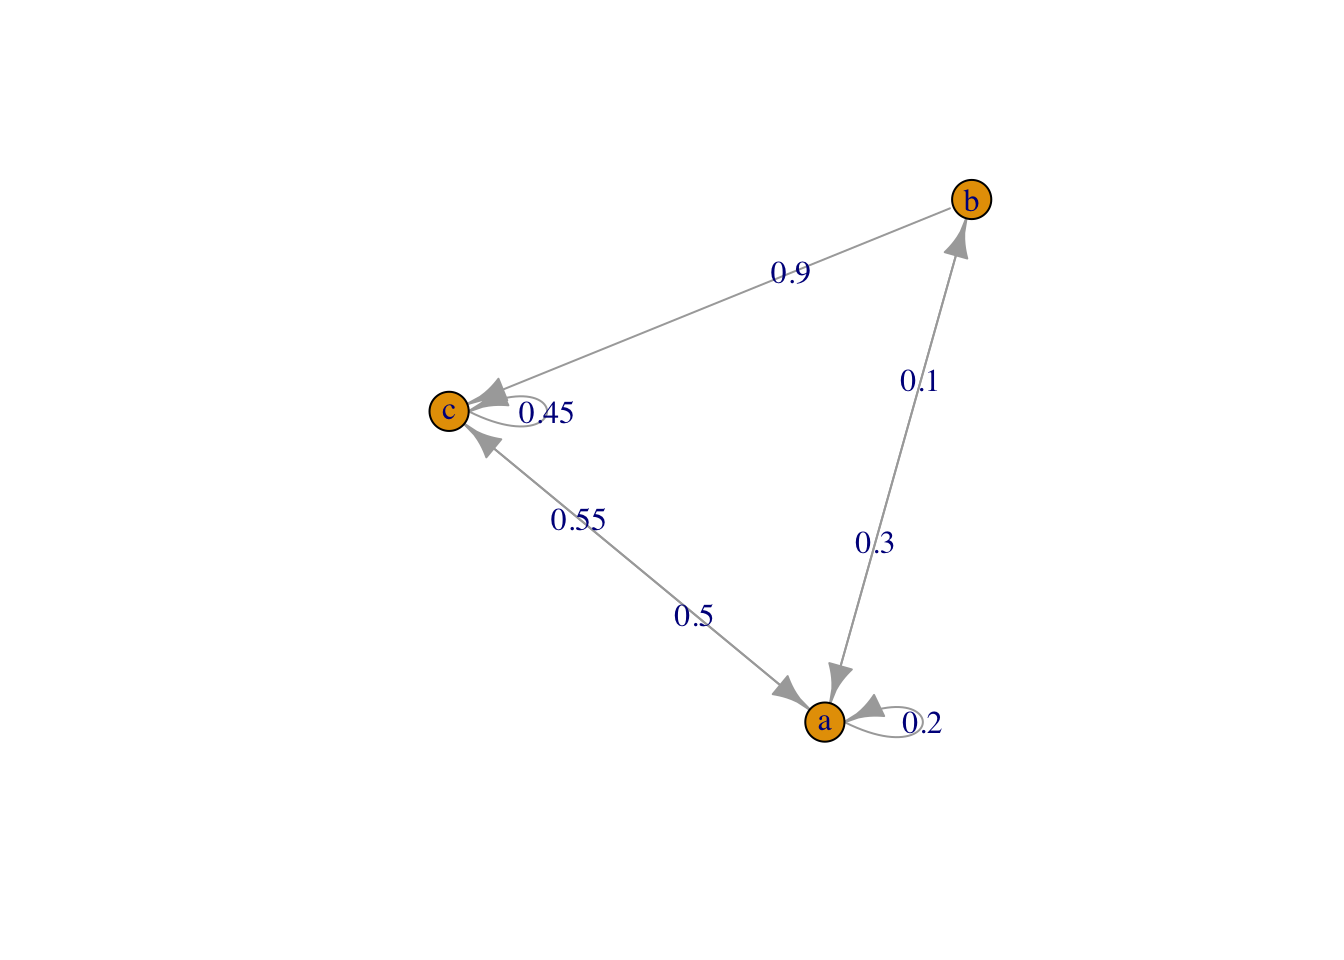
\includegraphics[width=0.95\linewidth]{02-CMTD_files/figure-latex/03-001-1} 

}

\caption{Grafo del proceso.}\label{fig:03-001}
\end{figure}

(2). Si la \(CMTD\) está en el estado \(c\) en el momento 17, ¿cuál es la probabilidad de que esté en el estado \(a\) en el momento 18?

\begin{itemize}
\tightlist
\item
  RESPUESTA: Nos preguntan por la probabilidad de transición para pasar, en un solo paso, del estado \(c\) (3) al estado \(a\) (1), por lo que viene dada por la componente \(p_{31}\) de la matriz de transición, es decir, 0.55.
\end{itemize}

\begin{whitebox}
Para resolver el cálculo con el ordenador basta utilizar la función \texttt{transitionProbability()}, con los argumentos: \texttt{object} (la cadena de markov), \texttt{t0} (el estado en el instante inicial), \texttt{t1} (el estado en el instante final).

\end{whitebox}

Así la pregunta (2) se responde con:

\begin{Shaded}
\begin{Highlighting}[]
\FunctionTok{transitionProbability}\NormalTok{(}\AttributeTok{object =}\NormalTok{ proceso, }\AttributeTok{t0 =} \StringTok{"c"}\NormalTok{, }\AttributeTok{t1 =} \StringTok{"a"}\NormalTok{)}
\end{Highlighting}
\end{Shaded}

\begin{verbatim}
## [1] 0.55
\end{verbatim}

(3). Si la \(CMTD\) está en el estado \(c\) en un momento dado, ¿cuál es la probabilidad de que esté en el estado \(a\) transcurridos tres unidades de tiempo? ¿y después de 10?

\begin{itemize}
\tightlist
\item
  RESPUESTA: Para resolver esta cuestión definimos el estado inicial y lo multiplicamos por la matriz de transición que corresponda, que en este caso, aplicando la Ecuación \eqref{eq:matriznpasos}, será \(P^n\), para \(n=3\) y \(n=10\). Obtendremos así la distribución de probabilidad en \(n\) transiciones, con la probabilidad de llegar a cada uno de los eventos posibles, \(\{a,b,c\}\) en \(n\), partiendo de un estado inicial dado.
\end{itemize}

\begin{Shaded}
\begin{Highlighting}[]
\CommentTok{\# Estado inicial en c}
\NormalTok{sini }\OtherTok{\textless{}{-}} \FunctionTok{c}\NormalTok{(}\DecValTok{0}\NormalTok{, }\DecValTok{0}\NormalTok{, }\DecValTok{1}\NormalTok{)}
\CommentTok{\# matriz de transición de 3 pasos}
\NormalTok{mt3 }\OtherTok{\textless{}{-}} \FunctionTok{ptran.n}\NormalTok{(pmat,}\DecValTok{3}\NormalTok{);mt3}
\end{Highlighting}
\end{Shaded}

\begin{verbatim}
##          a       b        c
## a 0.402250 0.10350 0.494250
## b 0.356250 0.15450 0.489250
## c 0.350625 0.10725 0.542125
\end{verbatim}

\begin{Shaded}
\begin{Highlighting}[]
\CommentTok{\# o bien extrayendo la matriz de transición del proceso}
\FunctionTok{ptran.n}\NormalTok{(proceso[}\DecValTok{1}\SpecialCharTok{:}\DecValTok{3}\NormalTok{,}\DecValTok{1}\SpecialCharTok{:}\DecValTok{3}\NormalTok{],}\DecValTok{3}\NormalTok{)}
\end{Highlighting}
\end{Shaded}

\begin{verbatim}
##          a       b        c
## a 0.402250 0.10350 0.494250
## b 0.356250 0.15450 0.489250
## c 0.350625 0.10725 0.542125
\end{verbatim}

\begin{Shaded}
\begin{Highlighting}[]
\CommentTok{\# Situación del proceso dentro de 3 instantes}
\NormalTok{sini}\SpecialCharTok{\%*\%}\NormalTok{mt3}
\end{Highlighting}
\end{Shaded}

\begin{verbatim}
##             a       b        c
## [1,] 0.350625 0.10725 0.542125
\end{verbatim}

\begin{Shaded}
\begin{Highlighting}[]
\CommentTok{\# matriz de transición de 10 pasos}
\NormalTok{mt10 }\OtherTok{\textless{}{-}}\FunctionTok{ptran.n}\NormalTok{(pmat,}\DecValTok{10}\NormalTok{)}
\CommentTok{\# Situación del proceso dentro de 10 instantes}
\NormalTok{sini}\SpecialCharTok{\%*\%}\NormalTok{mt10}
\end{Highlighting}
\end{Shaded}

\begin{verbatim}
##              a         b         c
## [1,] 0.3703899 0.1110948 0.5185153
\end{verbatim}

(4). ¿Cuál es la distribución de probabilidad del proceso transcurridos \(10\) instantes de tiempo desde el momento inicial del proceso, sea cual sea su estado?

\begin{itemize}
\tightlist
\item
  RESPUESTA: Si conocemos la distribución de probabilidad en el estado inicial, \(p(0)\), podemos obtener la distribución de probabilidad en \(n\) transiciones con la Ecuación \ref{ecu-distriproceso}:
\end{itemize}

\begin{Shaded}
\begin{Highlighting}[]
\DocumentationTok{\#\#\# Distribución de probabilidad del proceso dentro de 10 instantes}
\CommentTok{\# Distribución de  probabilidad inicial}
\NormalTok{dini }\OtherTok{\textless{}{-}} \FunctionTok{c}\NormalTok{(}\FloatTok{0.4}\NormalTok{, }\FloatTok{0.2}\NormalTok{, }\FloatTok{0.4}\NormalTok{)}
\CommentTok{\# matriz de transición de 10 pasos}
\NormalTok{mt10 }\OtherTok{\textless{}{-}} \FunctionTok{ptran.n}\NormalTok{(pmat,}\DecValTok{10}\NormalTok{)}
\CommentTok{\# distribución de probabilidad marginal en 10 pasos: inicial x condicional}
\NormalTok{dini}\SpecialCharTok{\%*\%}\NormalTok{mt10}
\end{Highlighting}
\end{Shaded}

\begin{verbatim}
##             a         b         c
## [1,] 0.370364 0.1111134 0.5185226
\end{verbatim}

En base a la distribución del proceso tras \(n=10\) pasos, apreciamos que lo más probable es que el sistema se ecuentre en el estado ``c'' (prob=0.52), y lo menos probable es que se encuentre en el estado ``b'' (prob=0.11).

(5). Corroborar los resultados analíticos obtenidos en (4) con simulaciones.

\begin{itemize}
\tightlist
\item
  RESPUESTA: Para ver el comportamiento de un proceso después de que transcurran \(n\) pasos habrá que simularlo durante \(n\) instantes de tiempo. Puesto que buscamos una estimación de lo que va a ocurrir en ese momento, simularemos \(nsim=100\) veces el proceso hasta el instante \(n=10\), nos quedaremos con el estado en que se encuentra el proceso en ese instante \(n\) y evaluaremos las probabilidades obtenidas para los tres estados \(\{a,b,c\}\). Los resultados serán más próximos a la solución analítica, cuanto mayor sea el número de simulaciones (prueba a modificar \(nsim\)).
\end{itemize}

\begin{whitebox}
Para simular una CMTD hasta una transición \(n\) con la librería \texttt{markovchain}
basta utilizar la función \texttt{rmarkovchain(n,\ proceso)}, donde proceso ha sido definido previamente con la función \texttt{new()}.

\end{whitebox}

\begin{Shaded}
\begin{Highlighting}[]
\DocumentationTok{\#\#\# Simulación del proceso para n=10 instantes }
\NormalTok{res}\OtherTok{=}\FunctionTok{vector}\NormalTok{()}
\NormalTok{nsim}\OtherTok{=}\DecValTok{100}
\NormalTok{n}\OtherTok{=}\DecValTok{10}
\ControlFlowTok{for}\NormalTok{(i }\ControlFlowTok{in} \DecValTok{1}\SpecialCharTok{:}\NormalTok{nsim)\{}
\NormalTok{  res[i]}\OtherTok{=}\FunctionTok{rmarkovchain}\NormalTok{(n, proceso)[n]\}}
\FunctionTok{prop.table}\NormalTok{(}\FunctionTok{table}\NormalTok{(res))}
\end{Highlighting}
\end{Shaded}

\begin{verbatim}
## res
##    a    b    c 
## 0.31 0.12 0.57
\end{verbatim}

\hypertarget{ExCMTD}{%
\section{Aplicaciones}\label{ExCMTD}}

Las aplicaciones de las CMTD son muy numerosas. A continuación presentamos una colección de ejemplos basados en aplicaciones prácticas de estos procesos, con algunos de los cuales trabajaremos a lo largo de la unidad.

\hypertarget{CM01}{%
\subsection{Colas de espera}\label{CM01}}

Supongamos una consulta médica en un centro de salud, en el que los pacientes que llegan se colocan en una única cola de espera, son atendidos consecutivamente y sólo se atiende a un paciente en cada periodo de 5 minutos. Consideramos las variables aleatorias:

\begin{itemize}
\tightlist
\item
  \(Y_n:\) Número de clientes que acuden a la consulta durante el n-ésimo periodo de servicio, con posibles valores \(\{0, 1, 2,...\}\) donde
\end{itemize}

\[Pr(Y_n = k) = a_k, \quad k=0, 1, 2,...; \quad 0 \leq a_k \leq 1; \quad \sum_{k=0}^{\infty} a_k =1\]

\begin{itemize}
\tightlist
\item
  \(X_n:\) Número de pacientes que hay esperando en la cola en el momento que empieza el n-ésimo periodo de servicio, con posibles valores \(\{0, 1, 2,...\}\), que conforman un proceso estocástico discreto con:
\end{itemize}

\begin{equation*}
X_{n+1} = 
\begin{cases}
Y_n & \text{ si } X_n = 0\\
X_n - 1 + Y_n & \text{ si } X_n \neq 0
\end{cases}
\end{equation*}

de forma que cada \(X_n\) sólo dependerá de lo que haya ocurrido en el periodo inmediatamente anterior, luego \(\{X_n, n \in \mathbb{N}\}\) es una \(CMTD\), con probabilidades de transición dadas por:

\begin{eqnarray*}
p_{0j} &=& Pr[X_{n+1} = j | X_{n} = 0] = Pr[Y_n = j] = a_j \\
p_{ij} &=&Pr[X_{n+1} = j | X_{n} = i] = Pr[i - 1 + Y_n = j] = a_{j-i+1}; \quad i\neq 0; \ j \geq i-1 \\
p_{ij} &=& 0; \quad j+1<i\neq0.
\end{eqnarray*}

La matriz de transición viene dada por:

\[P = 
\begin{pmatrix}
a_0 & a_1 & a_2 & a_3 &...& a_j & ...\\
a_0 & a_1 & a_2 & a_3 &...& a_j & ...\\
0 & a_0 & a_1 & a_2 &...& a_{j-1} & ...\\
0 & 0 & a_0 & a_1 &...& a_{j-2} & ...\\
... & ... & ... & ... &...& ... & ...
\end{pmatrix}\]

\hypertarget{fiabilidad}{%
\subsection{Fiabilidad de máquinas}\label{fiabilidad}}

La empresa \emph{Depend-On-Us} fabrica una máquina que está encendida o apagada (``On''/``Off''). Si está ``On'' al principio de un día, entonces está ``On'' al principio del día siguiente con una probabilidad de 0.98 (independientemente del historial de la máquina), o falla con una probabilidad de 0.02. Una vez que la máquina falla, la empresa envía a una persona para que la repare. Si la máquina está averiada al principio de un día, está ``Off'' al principio del día siguiente con una probabilidad de 0.03 (independientemente del historial de la máquina), o la reparación se completa y la máquina está ``On'' con probabilidad de 0.97. Una máquina reparada está como nueva.

Podemos modelar este sistema mediante una \(CMTD\) si consideramos la variable aleatoria \(X_n\) que refleja el estado de la máquina en el día \(n\) definida como:

\begin{equation*}
X_{n} = 
\begin{cases}
0 & \text{ Off}\\
1 & \text{ On}
\end{cases}
\end{equation*}

de forma que la matriz de transicción viene dada por:

\[P = 
\begin{pmatrix}
0.03 & 0.97\\
0.02 & 0.98
\end{pmatrix}\]

Supongamos ahora que la empresa mantiene dos máquinas de este tipo que son idénticas, se comportan de forma independiente y cada una tiene su propio reparador.

Sea \(Y_n\) el número de máquinas en estado ``On'' al principio del día \(n\), que constituye una CMTD cuyo espacio de estados es \(\{0, 1, 2\}\), puesto que la situación de las máquinas un día cualquiera sólo depende de cómo estaban el día anterior (cumplen la Ecuación \eqref{eq:cmtd}.

Calculemos la probabilidad de transición para un caso concreto: \(Y_n = i = 1\) e \(Y_{n+1} = j = 0\), que identifica una situación en la que una máquina está en funcionamiento y otra en paro el día \(n\), pero al día siguiente ambas están paradas. Así, la máquina que está ``Off'' el día \(n\) debe permanecer ``Off'' al día siguiente, y la máquina que está ``On'' debe cambiar a ``Off'' el día siguiente. Como las máquinas son independientes, la probabilidad de cambio de estado es:

\[p_{10}=Pr[Y_{n+1} = 0 | Y_n = 1] = 0.03 * 0.02 = 0.0006\] Procediendo de la misma forma obtenemos la matriz completa de transición de un paso del proceso como:

\[P = 
\begin{pmatrix}
0.0009 & 0.0582 & 0.9409\\
0.0006 & 0.0488 & 0.9506\\
0.0004 & 0.0392 & 0.9604
\end{pmatrix}\]

Representamos a continuación este sistema en forma de grafo en la Figura \ref{fig:03-009}. Para ello acudimos a la librería \texttt{markovchain}.

\begin{Shaded}
\begin{Highlighting}[]
\CommentTok{\# Definimos estados}
\NormalTok{estados }\OtherTok{\textless{}{-}} \FunctionTok{c}\NormalTok{(}\StringTok{"0"}\NormalTok{, }\StringTok{"1"}\NormalTok{, }\StringTok{"2"}\NormalTok{)}
\CommentTok{\# Matriz de transición }
\NormalTok{pmat }\OtherTok{\textless{}{-}} \FunctionTok{matrix}\NormalTok{(}\AttributeTok{data =} \FunctionTok{c}\NormalTok{(}\FloatTok{0.0009}\NormalTok{, }\FloatTok{0.0582}\NormalTok{, }\FloatTok{0.9409}\NormalTok{, }
                        \FloatTok{0.0006}\NormalTok{, }\FloatTok{0.0488}\NormalTok{, }\FloatTok{0.9506}\NormalTok{, }
                        \FloatTok{0.0004}\NormalTok{, }\FloatTok{0.0392}\NormalTok{, }\FloatTok{0.9604}\NormalTok{), }
               \AttributeTok{byrow =} \ConstantTok{TRUE}\NormalTok{, }\AttributeTok{nrow =} \DecValTok{3}\NormalTok{, }
               \AttributeTok{dimnames =} \FunctionTok{list}\NormalTok{(estados, estados))}
\CommentTok{\# CMTD}
\NormalTok{fiabilidad }\OtherTok{\textless{}{-}} \FunctionTok{new}\NormalTok{(}\StringTok{"markovchain"}\NormalTok{, }\AttributeTok{states =}\NormalTok{ estados, }
                 \AttributeTok{byrow =} \ConstantTok{TRUE}\NormalTok{, }\AttributeTok{transitionMatrix =}\NormalTok{ pmat, }
                 \AttributeTok{name =} \StringTok{"Fiabilidad"}\NormalTok{)}
\CommentTok{\# Verificamos los datos introducidos}
\NormalTok{fiabilidad}
\end{Highlighting}
\end{Shaded}

\begin{verbatim}
## Fiabilidad 
##  A  3 - dimensional discrete Markov Chain defined by the following states: 
##  0, 1, 2 
##  The transition matrix  (by rows)  is defined as follows: 
##       0      1      2
## 0 9e-04 0.0582 0.9409
## 1 6e-04 0.0488 0.9506
## 2 4e-04 0.0392 0.9604
\end{verbatim}

\begin{Shaded}
\begin{Highlighting}[]
\CommentTok{\# Diagrama}
\FunctionTok{plot}\NormalTok{(fiabilidad, }\AttributeTok{vertex.color=}\StringTok{"steelblue"}\NormalTok{, }
     \AttributeTok{vertex.label.font =} \DecValTok{2}\NormalTok{, }
     \AttributeTok{edge.label.size =} \FloatTok{0.1}\NormalTok{,}
     \AttributeTok{edge.arrow.size=}\FloatTok{0.5}\NormalTok{, }
     \AttributeTok{vertex.shape =} \StringTok{"rectangle"}\NormalTok{, }
     \AttributeTok{vertex.size =} \DecValTok{20}\NormalTok{)}
\end{Highlighting}
\end{Shaded}

\begin{figure}

{\centering 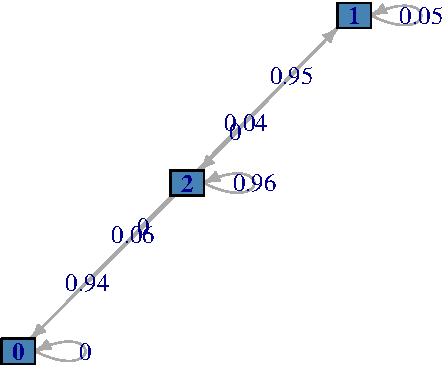
\includegraphics[width=0.95\linewidth]{02-CMTD_files/figure-latex/03-009-1} 

}

\caption{Diagrama del sistema de fiabilidad}\label{fig:03-009}
\end{figure}

\hypertarget{meteo}{%
\subsection{Meteorología}\label{meteo}}

El tiempo en la ciudad de Heavenly se clasifica como soleado, nublado o lluvioso. Supongamos que el tiempo de mañana depende sólo del tiempo de hoy de la siguiente manera: si hoy hace sol, mañana estará nublado con una probabilidad de 0.3 y lluvioso con probabilidad 0.2; si hoy está nublado, mañana estará soleado con probabilidad 0.5 y lluvioso con probabilidad 0.3; y finalmente, si hoy está lluvioso, mañana estará soleado con probabilidad 0.4 y nublado con probabilidad 0.5.

Consideramos la variable aleatoria \(X_n\) que registra las condiciones meteorológicas del día \(n\) como:

\begin{equation*}
X_{n} = 
\begin{cases}
1 & \text{ soleado}\\
2 & \text{ nublado}\\
3 & \text{ lluvioso}
\end{cases}
\end{equation*}

de forma que el proceso \(\{X_n, n \in \mathbb{N}\}\) con espacio de estados \(S = \{1, 2, 3\}\) se puede considerar como una \(CMTD\), cuya matriz de transición se puede obtener de forma muy rápida como:

\[P = 
\begin{pmatrix}
0.50 & 0.30 & 0.20\\
0.50 & 0.20 & 0.30\\
0.40 & 0.50 & 0.10
\end{pmatrix}\]

Representamos a continuación este sistema en forma de grafo en la Figura \ref{fig:03-011}.

\begin{Shaded}
\begin{Highlighting}[]
\CommentTok{\# Definimos estados}
\NormalTok{estados }\OtherTok{\textless{}{-}} \FunctionTok{c}\NormalTok{(}\StringTok{"Soleado"}\NormalTok{, }\StringTok{"Nublado"}\NormalTok{, }\StringTok{"LLuvioso"}\NormalTok{)}
\CommentTok{\# Matriz de transición }
\NormalTok{pmat }\OtherTok{\textless{}{-}} \FunctionTok{matrix}\NormalTok{(}\AttributeTok{data =} \FunctionTok{c}\NormalTok{(}\FloatTok{0.50}\NormalTok{, }\FloatTok{0.30}\NormalTok{, }\FloatTok{0.20}\NormalTok{, }
                        \FloatTok{0.50}\NormalTok{, }\FloatTok{0.20}\NormalTok{, }\FloatTok{0.30}\NormalTok{, }
                        \FloatTok{0.40}\NormalTok{, }\FloatTok{0.50}\NormalTok{, }\FloatTok{0.10}\NormalTok{), }
               \AttributeTok{byrow =} \ConstantTok{TRUE}\NormalTok{, }\AttributeTok{nrow =} \DecValTok{3}\NormalTok{, }
               \AttributeTok{dimnames =} \FunctionTok{list}\NormalTok{(estados, estados))}
\CommentTok{\# CMTD}
\NormalTok{meteo }\OtherTok{\textless{}{-}} \FunctionTok{new}\NormalTok{(}\StringTok{"markovchain"}\NormalTok{, }\AttributeTok{states =}\NormalTok{ estados, }
                 \AttributeTok{byrow =} \ConstantTok{TRUE}\NormalTok{, }\AttributeTok{transitionMatrix =}\NormalTok{ pmat, }
             \AttributeTok{name =} \StringTok{"Meteorología"}\NormalTok{)}
\CommentTok{\# Verificamos los datos introducidos}
\NormalTok{meteo}
\end{Highlighting}
\end{Shaded}

\begin{verbatim}
## Meteorología 
##  A  3 - dimensional discrete Markov Chain defined by the following states: 
##  Soleado, Nublado, LLuvioso 
##  The transition matrix  (by rows)  is defined as follows: 
##          Soleado Nublado LLuvioso
## Soleado      0.5     0.3      0.2
## Nublado      0.5     0.2      0.3
## LLuvioso     0.4     0.5      0.1
\end{verbatim}

\begin{Shaded}
\begin{Highlighting}[]
\CommentTok{\# Diagrama}
\FunctionTok{plot}\NormalTok{(meteo, }\AttributeTok{vertex.color=}\StringTok{"steelblue"}\NormalTok{, }
     \AttributeTok{vertex.label.font =} \DecValTok{2}\NormalTok{, }
     \AttributeTok{edge.label.size =} \FloatTok{0.1}\NormalTok{,}
     \AttributeTok{edge.arrow.size=}\FloatTok{0.5}\NormalTok{, }
     \AttributeTok{vertex.shape =} \StringTok{"rectangle"}\NormalTok{, }
     \AttributeTok{vertex.size =} \DecValTok{60}\NormalTok{)}
\end{Highlighting}
\end{Shaded}

\begin{figure}

{\centering 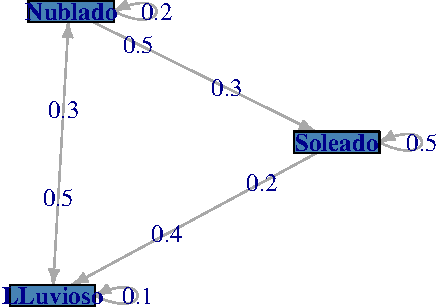
\includegraphics[width=0.95\linewidth]{02-CMTD_files/figure-latex/03-011-1} 

}

\caption{Diagrama del sistema de metereología}\label{fig:03-011}
\end{figure}

\hypertarget{inventario}{%
\subsection{Problema de inventario}\label{inventario}}

Computers-R-Us almacena una amplia variedad de PCs para la venta al por menor. La tienda abre de lunes a viernes de 8:00 a.m. a 5:00 p.m., y utiliza la siguiente política operativa para controlar el inventario al inicio de semana, en función del número de PCs que quedan en stock el viernes de la semana anterior a las 5:00 p.m:

\begin{itemize}
\item
  Si el stock al finalizar una semana es inferior a dos, se piden suficientes ordenadores para disponer de un stock total de cinco al inicio la semana siguiente.
\item
  Si el stock al final de la semana es de dos o más, no se realiza ningún pedido.
\end{itemize}

La demanda de ordenadores durante la semana es una variable aleatoria de Poisson con media 3. Cualquier demanda que no pueda ser satisfecha inmediatamente se pierde.

Se consideran las variables aleatorias:

\begin{itemize}
\tightlist
\item
  \(X_n:\) número de PCs en stock a las 8:00 a.m del lunes de la semana \(n\).
\item
  \(D_n:\) número de PCs demandados durante la semana \(n\).
\end{itemize}

De esta forma el número de Pcs que hay en la tienda al inicio de la semana \(n+1\) viene dado por los que habían en stock al inicio de la semana anterior menos los que se han vendido, siempre que dicho balance sea al menos de 2 unidades, y será de 5 en otro caso:

\begin{equation*}
X_{n+1} = 
\begin{cases}
X_n - D_n & \text{ si } X_n - D_n \geq 2\\
5 & \text{ si } X_n - D_n < 2
\end{cases}
\end{equation*}

Necesariamente entonces, \(X_{n+1} \geq X_n\) dado que \(D_n \geq 0\).

Se trata de una CMTD con espacio de estados \(\{2, 3, 4, 5\}\), puesto que el estado del sistema en la semana \(n+1\) sólo depende de su estado en la semana anterior \(n\). Calculemos las probabilidades de transición.

\begin{itemize}
\tightlist
\item
  Para \(j= 2, 3, 4\)
\end{itemize}

\[\begin{array}{ll}
Pr[X_{n+1}  = j | X_n = i] & = Pr[X_n - D_n = j | X_n = i]\\
& = Pr[D_n=X_n-j | X_n = i]\\
& = Pr[D_n = i - j] \\
&=\begin{cases}
Pr[D_n = i - j] \quad \text{ si } i\geq j \\
0 \qquad \qquad \qquad \quad \text{ si } i< j
\end{cases}
\end{array}\]

\begin{itemize}
\tightlist
\item
  Para \(j=5\) e \(5>i\geq 2\)
\end{itemize}

\[\begin{array}{ll}
Pr[X_{n+1}  = 5 | X_n = i] & = Pr[X_n - D_n \leq 1 | X_n = i]\\
&=Pr[D_n \geq X_n-1|X_n=i] \\
& = Pr(D_n \geq i - 1).
\end{array}\]

\begin{itemize}
\tightlist
\item
  Para \(j=5\) e \(i=5\), podría ocurrir que durante la semana anterior no se hubiera vendido nada \(D_n=0\) o se hubieran vendido al menos cuatro ordenadores, \(D_n \geq 4\) (para dejar un stock inferior a 2),
\end{itemize}

\[\begin{array}{ll}
Pr[X_{n+1}  = 5 | X_n = 5] & = Pr[X_n - D_n =5 | X_n = 5]\\
&=Pr[D_n =0] + Pr(D_n \geq 4).
\end{array}\]

Usando el hecho de que la variable \(D_n \sim Po(3)\) podemos obtener la tabla de probabilidades siguientes:

\begin{longtable}[]{@{}llllll@{}}
\toprule
\(k\) & 0 & 1 & 2 & 3 & 4 \\
\midrule
\endhead
\(Pr[D_n = k]\) & 0.0498 & 0.1494 & 0.2240 & 0.2240 & 0.1680 \\
\(Pr[D_n \geq k]\) & 1.0000 & 0.9502 & 0.8008 & 0.5768 & 0.3528 \\
\bottomrule
\end{longtable}

Usando los datos de esta tabla calculamos fácilmente la matriz de transición asociada a la \(CMTD\) como:

\[P = 
\begin{pmatrix}
0.0498 & 0 & 0 & 0.9502\\
0.1494 & 0.0498 & 0 & 0.8008\\
0.2240 & 0.1494 & 0.0498 & 0.5768\\
0.2240 & 0.2240 & 0.1494 & 0.4026
\end{pmatrix}\]

Representamos a continuación este sistema en forma de grafo en la Figura \ref{fig:03-013}.

\begin{Shaded}
\begin{Highlighting}[]
\CommentTok{\# Definimos estados}
\NormalTok{estados }\OtherTok{\textless{}{-}} \FunctionTok{c}\NormalTok{(}\StringTok{"2 PCs"}\NormalTok{, }\StringTok{"3 PCs"}\NormalTok{, }\StringTok{"4 PCs"}\NormalTok{, }\StringTok{"5 PCs"}\NormalTok{)}
\CommentTok{\# Matriz de transición }
\NormalTok{pmat }\OtherTok{\textless{}{-}} \FunctionTok{matrix}\NormalTok{(}\AttributeTok{data =} \FunctionTok{c}\NormalTok{(}\FloatTok{0.0498}\NormalTok{, }\DecValTok{0}\NormalTok{, }\DecValTok{0}\NormalTok{, }\FloatTok{0.9502}\NormalTok{, }
                        \FloatTok{0.1494}\NormalTok{, }\FloatTok{0.0498}\NormalTok{, }\DecValTok{0}\NormalTok{, }\FloatTok{0.8008}\NormalTok{,  }
                        \FloatTok{0.2240}\NormalTok{, }\FloatTok{0.1494}\NormalTok{, }\FloatTok{0.0498}\NormalTok{, }\FloatTok{0.5768}\NormalTok{,}
                        \FloatTok{0.2240}\NormalTok{, }\FloatTok{0.2240}\NormalTok{, }\FloatTok{0.1494}\NormalTok{, }\FloatTok{0.4026}\NormalTok{), }
               \AttributeTok{byrow =} \ConstantTok{TRUE}\NormalTok{, }\AttributeTok{nrow =} \DecValTok{4}\NormalTok{, }
               \AttributeTok{dimnames =} \FunctionTok{list}\NormalTok{(estados, estados))}
\CommentTok{\# CMTD}
\NormalTok{inventario }\OtherTok{\textless{}{-}} \FunctionTok{new}\NormalTok{(}\StringTok{"markovchain"}\NormalTok{, }\AttributeTok{states =}\NormalTok{ estados, }
                 \AttributeTok{byrow =} \ConstantTok{TRUE}\NormalTok{, }\AttributeTok{transitionMatrix =}\NormalTok{ pmat, }
                 \AttributeTok{name =} \StringTok{"inventario"}\NormalTok{)}
\CommentTok{\# Verificamos los datos introducidos}
\NormalTok{inventario}
\end{Highlighting}
\end{Shaded}

\begin{verbatim}
## inventario 
##  A  4 - dimensional discrete Markov Chain defined by the following states: 
##  2 PCs, 3 PCs, 4 PCs, 5 PCs 
##  The transition matrix  (by rows)  is defined as follows: 
##        2 PCs  3 PCs  4 PCs  5 PCs
## 2 PCs 0.0498 0.0000 0.0000 0.9502
## 3 PCs 0.1494 0.0498 0.0000 0.8008
## 4 PCs 0.2240 0.1494 0.0498 0.5768
## 5 PCs 0.2240 0.2240 0.1494 0.4026
\end{verbatim}

\begin{Shaded}
\begin{Highlighting}[]
\CommentTok{\# Diagrama}
\FunctionTok{plot}\NormalTok{(inventario, }\AttributeTok{vertex.color=}\StringTok{"steelblue"}\NormalTok{, }
     \AttributeTok{vertex.label.font =} \DecValTok{2}\NormalTok{, }
     \AttributeTok{edge.label.size =} \FloatTok{0.1}\NormalTok{,}
     \AttributeTok{edge.arrow.size=}\FloatTok{0.5}\NormalTok{, }
     \AttributeTok{vertex.shape =} \StringTok{"rectangle"}\NormalTok{, }
     \AttributeTok{vertex.size =} \DecValTok{40}\NormalTok{)}
\end{Highlighting}
\end{Shaded}

\begin{figure}

{\centering 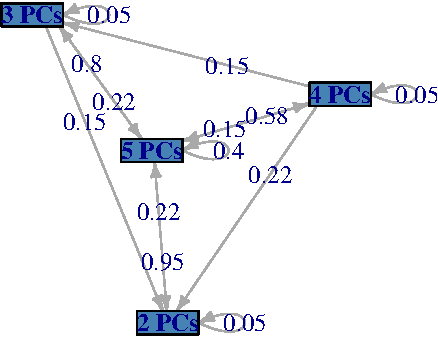
\includegraphics[width=0.95\linewidth]{02-CMTD_files/figure-latex/03-013-1} 

}

\caption{Diagrama del sistema de inventario}\label{fig:03-013}
\end{figure}

\hypertarget{planificacion}{%
\subsection{Planificación de mano de obra}\label{planificacion}}

Paper Pushers, Inc.~es una empresa de seguros que emplea a 100 trabajadores organizados en cuatro grados, etiquetados como \(1\), \(2\), \(3\) y \(4\). Por razones de simplicidad, supondremos que los trabajadores pueden ser promovidos de un grado a otro, o dejar la empresa, sólo al principio de la semana. Un trabajador en el grado 1 al principio de la semana asciende al grado 2 con probabilidad 0.03, deja la empresa con una probabilidad de 0.02, o continúa en el mismo grado al principio de la semana siguiente. Un trabajador que se encuentra en el grado 2 al principio de la semana asciende al grado 3 con probabilidad 0.01, abandona la empresa con probabilidad 0.008 o continúa en el mismo grado al principio de la semana siguiente. Un trabajador de grado 3 al principio de la semana asciende al grado 4 con una probabilidad de 0.005, abandona la empresa con una probabilidad de 0.02, o continúa en el mismo grado al principio de la semana siguiente. Un trabajador que se encuentra en el grado 4 al principio de la semana deja la empresa con una probabilidad de 0.01 o continúa en el mismo grado al principio de la semana siguiente. Si un trabajador abandona la empresa, es sustituido instantáneamente por otro de grado 1. El movimiento de los trabajadores dentro de la empresa puede modelizarse utilizando una \(CMTD\).

Supondremos que todos los ascensos de los trabajadores se deciden de manera independiente. Esto simplifica considerablemente nuestro modelo. En lugar de hacer un seguimiento de los 100 trabajadores, tenemos en cuenta a un único trabajador, digamos el trabajador \(k\), donde \(k = 1, 2,...,100\). Pensamos en \(k\) como un ID de trabajador, y cuando este trabajador deja la empresa, se le asigna al nuevo sustituto. Sea \(X_n^k\) el grado en el que se encuentra el trabajador \(k\) al principio de la n-ésima semana. Ahora, si suponemos que los ascensos de los trabajadores se determinan independientemente del historial del trabajador (es decir, que el tiempo transcurrido en un grado determinado no afecta a las posibilidades de promoción), vemos que para \(k = 1, 2,...,100\) el conjunto \(\{X_n^k, n \in \mathbb{N}\}\) es una \(CMTD\) con espacio de estados \(S =\{1, 2, 3, 4\}\).

Para obtener la matriz de transiciones procedemos con un ejemplo. Supongamos que \(X_n^k = 3\) entonces:

\begin{itemize}
\tightlist
\item
  Si es promocionado (\(X_{n+1}^k = 4\)), tenemos que \(Pr[X_{n+1}^k = 4 | X_n^k = 3] = 0.005.\)
\item
  Si deja la empresa, es reemplazado por un nuevo empleado de grado 1 (\(X_{n+1}^k = 1\)) de forma que \(Pr[X_{n+1}^k = 1 | X_n^k = 3] = 0.02.\)
\item
  Si se mantiene en el mismo puesto, tenemos que \(Pr[X_{n+1}^k = 3 | X_n^k = 3] = 0.975.\)
\end{itemize}

Procediendo de forma similar en el resto de situaciones tenemos la matriz de transición para cualquiera de los trabajadores como:

\[P = 
\begin{pmatrix}
0.970 & 0.030 & 0 & 0\\
0.008 & 0.982 & 0.010 & 0\\
0.020 & 0 & 0.975 & 0.005\\
0.010 & 0 & 0 & 0.990
\end{pmatrix}\]

Representamos a continuación este sistema en forma de grafo en la Figura \ref{fig:03-017}.

\begin{Shaded}
\begin{Highlighting}[]
\CommentTok{\# Definimos estados}
\NormalTok{estados }\OtherTok{\textless{}{-}} \FunctionTok{c}\NormalTok{(}\StringTok{"1"}\NormalTok{, }\StringTok{"2"}\NormalTok{, }\StringTok{"3"}\NormalTok{, }\StringTok{"4"}\NormalTok{)}
\CommentTok{\# Matriz de transición }
\NormalTok{pmat }\OtherTok{\textless{}{-}} \FunctionTok{matrix}\NormalTok{(}\AttributeTok{data =} \FunctionTok{c}\NormalTok{(}\FloatTok{0.9700}\NormalTok{, }\FloatTok{0.0300}\NormalTok{, }\DecValTok{0}\NormalTok{, }\DecValTok{0}\NormalTok{, }
                        \FloatTok{0.0080}\NormalTok{, }\FloatTok{0.9820}\NormalTok{, }\FloatTok{0.0100}\NormalTok{, }\DecValTok{0}\NormalTok{,   }
                        \FloatTok{0.0200}\NormalTok{, }\DecValTok{0}\NormalTok{, }\FloatTok{0.9750}\NormalTok{, }\FloatTok{0.0050}\NormalTok{,}
                        \FloatTok{0.0100}\NormalTok{, }\DecValTok{0}\NormalTok{, }\DecValTok{0}\NormalTok{, }\FloatTok{0.9900}\NormalTok{), }
               \AttributeTok{byrow =} \ConstantTok{TRUE}\NormalTok{, }\AttributeTok{nrow =} \DecValTok{4}\NormalTok{, }
               \AttributeTok{dimnames =} \FunctionTok{list}\NormalTok{(estados, estados))}
\CommentTok{\# CMTD}
\NormalTok{planificacion }\OtherTok{\textless{}{-}} \FunctionTok{new}\NormalTok{(}\StringTok{"markovchain"}\NormalTok{, }\AttributeTok{states =}\NormalTok{ estados, }
                 \AttributeTok{byrow =} \ConstantTok{TRUE}\NormalTok{, }\AttributeTok{transitionMatrix =}\NormalTok{ pmat, }
                 \AttributeTok{name =} \StringTok{"planificacion"}\NormalTok{)}
\CommentTok{\# Verificamos los datos introducidos}
\NormalTok{planificacion}
\end{Highlighting}
\end{Shaded}

\begin{verbatim}
## planificacion 
##  A  4 - dimensional discrete Markov Chain defined by the following states: 
##  1, 2, 3, 4 
##  The transition matrix  (by rows)  is defined as follows: 
##       1     2     3     4
## 1 0.970 0.030 0.000 0.000
## 2 0.008 0.982 0.010 0.000
## 3 0.020 0.000 0.975 0.005
## 4 0.010 0.000 0.000 0.990
\end{verbatim}

\begin{Shaded}
\begin{Highlighting}[]
\CommentTok{\# Diagrama}
\FunctionTok{plot}\NormalTok{(planificacion, }\AttributeTok{vertex.color=}\StringTok{"steelblue"}\NormalTok{, }
     \AttributeTok{vertex.label.font =} \DecValTok{2}\NormalTok{, }
     \AttributeTok{vertex.label.color =} \StringTok{"white"}\NormalTok{,}
     \AttributeTok{edge.label.size =} \FloatTok{0.2}\NormalTok{,}
     \AttributeTok{edge.arrow.size=}\FloatTok{0.5}\NormalTok{, }
     \AttributeTok{vertex.shape =} \StringTok{"rectangle"}\NormalTok{,}
     \AttributeTok{vertex.size =} \DecValTok{20}\NormalTok{)}
\end{Highlighting}
\end{Shaded}

\begin{figure}

{\centering 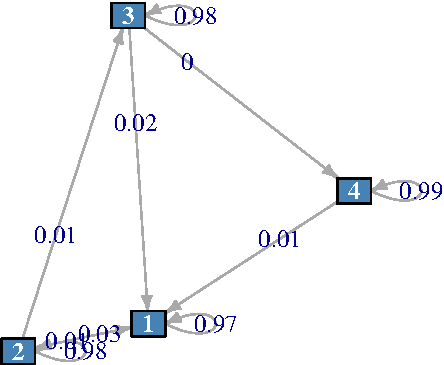
\includegraphics[width=0.95\linewidth]{02-CMTD_files/figure-latex/03-017-1} 

}

\caption{Diagrama del sistema de planificación}\label{fig:03-017}
\end{figure}

\hypertarget{mercadovalores}{%
\subsection{Mercado de valores}\label{mercadovalores}}

Las acciones ordinarias de la empresa Gadgets-R-Us se cotizan en el mercado de valores. El director financiero de Gadgets-R-Us compra y vende las acciones de su propia empresa para que el precio nunca baje de 2 dólares y nunca supere los 10 dólares (cuando esto ocurre, vende). Para simplificar, suponemos que \(X_n\), es el precio de cada acción al final del día \(n\), y sólo toma valores enteros; es decir, el espacio de estados del proceso \(\{X_n, n \in \mathbb{N}\}\) es \(S = 2, 3,...,10\). Si denominamos \(I_{n+1}\) al movimiento potencial del precio de las acciones en el día \(n+1\) en ausencia de cualquier intervención del director financiero, entonces tenemos que:

\begin{equation*}
X_{n+1} =  
\begin{cases}
2 & \text{ si } X_n + I_{n+1} \leq 2\\
X_n + I_{n+1} & \text{ si } 2 < X_n + I_{n+1} < 10\\
10 & \text{ si }  X_n + I_{n+1} \geq 10
\end{cases}
\end{equation*}

Un análisis continuado de los datos del pasado sugiere que los movimientos potenciales \(\{I_n, n \geq 1\}\) son una secuencia de variables iid con función de masa de probabilidad dada por:

\[Pr(I_n = k) = 0.2, \quad k = -2, -1, 0, 1, 2.\]

Esto implica que \(\{X_n, n \in \mathbb{N}\}\) es una \(CMTD\) con espacio de estados \(S = \{2, 3,...,10\}\), donde las probabilidades de transición se pueden obtener de forma sencilla. A modo de ejemplo presentamos los tres casos siguientes:

\[\begin{array}{ll}
Pr[X_{n+1} = 2 | X_n = 3] & = Pr[X_n + I_{n+1} \leq 2 | X_n = 3]\\
& = Pr[I_{n+1} \leq -1]= 0.4
\end{array}\]

\[\begin{array}{ll}
Pr[X_{n+1} = 6 | X_n = 5] & = Pr[X_n + I_{n+1} = 6 | X_n = 5]\\
& = Pr[I_{n+1} = 1]  = 0.2
\end{array}\]

\[\begin{array}{ll}
Pr[X_{n+1} = 10 | X_n = 10] & = Pr[X_n + I_{n+1} \geq 10 | X_n = 10]\\
& = Pr[I_{n+1} \geq 0] = 0.6
\end{array}\]

de forma que la matriz de transición del sistema viene dada por:

\[P = 
\begin{pmatrix}
0.6 & 0.2 & 0.2 & 0 & 0 & 0 & 0 & 0 & 0\\
0.4 & 0.2 & 0.2 & 0.2 & 0 & 0 & 0 & 0 & 0\\
0.2 & 0.2 & 0.2 & 0.2 & 0.2 & 0 & 0 & 0 & 0\\
0 & 0.2 & 0.2 & 0.2 & 0.2 & 0.2 & 0 & 0 & 0\\
0 & 0 & 0.2 & 0.2 & 0.2 & 0.2 & 0.2 & 0 & 0\\
0 & 0 & 0 & 0.2 & 0.2 & 0.2 & 0.2 & 0.2 & 0\\
0 & 0 & 0 & 0 & 0.2 & 0.2 & 0.2 & 0.2 & 0.2\\
0 & 0 & 0 & 0 & 0 & 0.2 & 0.2 & 0.2 & 0.4\\
0 & 0 & 0 & 0 & 0 & 0 & 0.2 & 0.2 & 0.6
\end{pmatrix}\]

Representamos a continuación este sistema en forma de grafo en la Figura \ref{fig:03-019}.

\begin{Shaded}
\begin{Highlighting}[]
\CommentTok{\# Definimos estados}
\NormalTok{estados }\OtherTok{\textless{}{-}} \FunctionTok{c}\NormalTok{(}\StringTok{"2"}\NormalTok{, }\StringTok{"3"}\NormalTok{, }\StringTok{"4"}\NormalTok{, }\StringTok{"5"}\NormalTok{, }\StringTok{"6"}\NormalTok{, }\StringTok{"7"}\NormalTok{, }\StringTok{"8"}\NormalTok{, }\StringTok{"9"}\NormalTok{, }\StringTok{"10"}\NormalTok{)}
\CommentTok{\# Matriz de transición }
\NormalTok{pmat }\OtherTok{\textless{}{-}} \FunctionTok{matrix}\NormalTok{(}\AttributeTok{data =} \FunctionTok{c}\NormalTok{(}\FloatTok{0.6}\NormalTok{ , }\FloatTok{0.2}\NormalTok{ , }\FloatTok{0.2}\NormalTok{ , }\DecValTok{0}\NormalTok{ , }\DecValTok{0}\NormalTok{ , }\DecValTok{0}\NormalTok{ , }\DecValTok{0}\NormalTok{ , }\DecValTok{0}\NormalTok{ , }\DecValTok{0}\NormalTok{,}
                        \FloatTok{0.4}\NormalTok{ , }\FloatTok{0.2}\NormalTok{ , }\FloatTok{0.2}\NormalTok{ , }\FloatTok{0.2}\NormalTok{ , }\DecValTok{0}\NormalTok{ , }\DecValTok{0}\NormalTok{ , }\DecValTok{0}\NormalTok{ , }\DecValTok{0}\NormalTok{ , }\DecValTok{0}\NormalTok{,}
                        \FloatTok{0.2}\NormalTok{ , }\FloatTok{0.2}\NormalTok{ , }\FloatTok{0.2}\NormalTok{ , }\FloatTok{0.2}\NormalTok{ , }\FloatTok{0.2}\NormalTok{ , }\DecValTok{0}\NormalTok{ , }\DecValTok{0}\NormalTok{ , }\DecValTok{0}\NormalTok{ , }\DecValTok{0}\NormalTok{,}
                        \DecValTok{0}\NormalTok{ , }\FloatTok{0.2}\NormalTok{ , }\FloatTok{0.2}\NormalTok{ , }\FloatTok{0.2}\NormalTok{ , }\FloatTok{0.2}\NormalTok{ , }\FloatTok{0.2}\NormalTok{ , }\DecValTok{0}\NormalTok{ , }\DecValTok{0}\NormalTok{ , }\DecValTok{0}\NormalTok{,}
                        \DecValTok{0}\NormalTok{ , }\DecValTok{0}\NormalTok{ , }\FloatTok{0.2}\NormalTok{ , }\FloatTok{0.2}\NormalTok{ , }\FloatTok{0.2}\NormalTok{ , }\FloatTok{0.2}\NormalTok{ , }\FloatTok{0.2}\NormalTok{ , }\DecValTok{0}\NormalTok{ , }\DecValTok{0}\NormalTok{,}
                        \DecValTok{0}\NormalTok{ , }\DecValTok{0}\NormalTok{ , }\DecValTok{0}\NormalTok{ , }\FloatTok{0.2}\NormalTok{ , }\FloatTok{0.2}\NormalTok{ , }\FloatTok{0.2}\NormalTok{ , }\FloatTok{0.2}\NormalTok{ , }\FloatTok{0.2}\NormalTok{ , }\DecValTok{0}\NormalTok{,}
                        \DecValTok{0}\NormalTok{ , }\DecValTok{0}\NormalTok{ , }\DecValTok{0}\NormalTok{ , }\DecValTok{0}\NormalTok{ , }\FloatTok{0.2}\NormalTok{ , }\FloatTok{0.2}\NormalTok{ , }\FloatTok{0.2}\NormalTok{ , }\FloatTok{0.2}\NormalTok{ , }\FloatTok{0.2}\NormalTok{,}
                        \DecValTok{0}\NormalTok{ , }\DecValTok{0}\NormalTok{ , }\DecValTok{0}\NormalTok{ , }\DecValTok{0}\NormalTok{ , }\DecValTok{0}\NormalTok{ , }\FloatTok{0.2}\NormalTok{ , }\FloatTok{0.2}\NormalTok{ , }\FloatTok{0.2}\NormalTok{ , }\FloatTok{0.4}\NormalTok{,}
                        \DecValTok{0}\NormalTok{ , }\DecValTok{0}\NormalTok{ , }\DecValTok{0}\NormalTok{ , }\DecValTok{0}\NormalTok{ , }\DecValTok{0}\NormalTok{ , }\DecValTok{0}\NormalTok{ , }\FloatTok{0.2}\NormalTok{ , }\FloatTok{0.2}\NormalTok{ , }\FloatTok{0.6}\NormalTok{), }
               \AttributeTok{byrow =} \ConstantTok{TRUE}\NormalTok{, }\AttributeTok{nrow =} \DecValTok{9}\NormalTok{, }
               \AttributeTok{dimnames =} \FunctionTok{list}\NormalTok{(estados, estados))}
\CommentTok{\# CMTD}
\NormalTok{mercado.valores }\OtherTok{\textless{}{-}} \FunctionTok{new}\NormalTok{(}\StringTok{"markovchain"}\NormalTok{, }\AttributeTok{states =}\NormalTok{ estados, }
                 \AttributeTok{byrow =} \ConstantTok{TRUE}\NormalTok{, }\AttributeTok{transitionMatrix =}\NormalTok{ pmat, }
                 \AttributeTok{name =} \StringTok{"Mercado de valores"}\NormalTok{)}
\CommentTok{\# Verificamos los datos introducidos}
\NormalTok{mercado.valores}
\end{Highlighting}
\end{Shaded}

\begin{verbatim}
## Mercado de valores 
##  A  9 - dimensional discrete Markov Chain defined by the following states: 
##  2, 3, 4, 5, 6, 7, 8, 9, 10 
##  The transition matrix  (by rows)  is defined as follows: 
##      2   3   4   5   6   7   8   9  10
## 2  0.6 0.2 0.2 0.0 0.0 0.0 0.0 0.0 0.0
## 3  0.4 0.2 0.2 0.2 0.0 0.0 0.0 0.0 0.0
## 4  0.2 0.2 0.2 0.2 0.2 0.0 0.0 0.0 0.0
## 5  0.0 0.2 0.2 0.2 0.2 0.2 0.0 0.0 0.0
## 6  0.0 0.0 0.2 0.2 0.2 0.2 0.2 0.0 0.0
## 7  0.0 0.0 0.0 0.2 0.2 0.2 0.2 0.2 0.0
## 8  0.0 0.0 0.0 0.0 0.2 0.2 0.2 0.2 0.2
## 9  0.0 0.0 0.0 0.0 0.0 0.2 0.2 0.2 0.4
## 10 0.0 0.0 0.0 0.0 0.0 0.0 0.2 0.2 0.6
\end{verbatim}

\begin{Shaded}
\begin{Highlighting}[]
\CommentTok{\# Diagrama}
\FunctionTok{plot}\NormalTok{(mercado.valores, }\AttributeTok{vertex.color=}\StringTok{"steelblue"}\NormalTok{, }
     \AttributeTok{vertex.label.font =} \DecValTok{2}\NormalTok{, }
     \AttributeTok{vertex.label.color =} \StringTok{"white"}\NormalTok{,}
     \AttributeTok{edge.label.size =} \FloatTok{0.2}\NormalTok{,}
     \AttributeTok{edge.arrow.size=}\FloatTok{0.5}\NormalTok{, }
     \AttributeTok{vertex.shape =} \StringTok{"rectangle"}\NormalTok{,}
     \AttributeTok{vertex.size =} \DecValTok{20}\NormalTok{)}
\end{Highlighting}
\end{Shaded}

\begin{figure}

{\centering 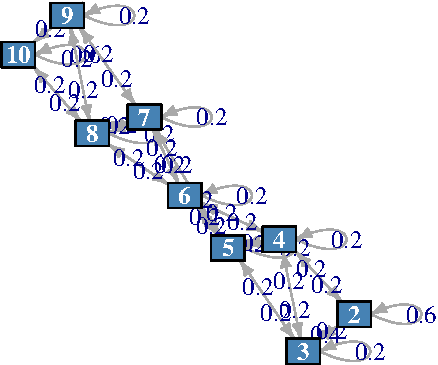
\includegraphics[width=0.95\linewidth]{02-CMTD_files/figure-latex/03-019-1} 

}

\caption{Diagrama del sistema del Mercado de valores}\label{fig:03-019}
\end{figure}

\hypertarget{telecomunicaciones}{%
\subsection{Telecomunicaciones}\label{telecomunicaciones}}

La empresa Tel-All Switch Corporation fabrica equipos de conmutación para redes de comunicación. Las redes de comunicación mueven los datos de un conmutador a otro a la velocidad del rayo en forma de paquetes, es decir, mediante cadenas de ceros y unos (llamadas bits). Los conmutadores Tel-All manejan paquetes de datos de longitud constante, es decir, el mismo número de bits en cada paquete. A nivel conceptual podemos pensar en el conmutador como un dispositivo de almacenamiento donde los paquetes llegan desde la red de usuarios según un proceso aleatorio, se almacenan en un buffer con capacidad para almacenar \(K\) paquetes y se eliminan del buffer uno a uno según un protocolo preestablecido. Uno de los protocolos utilizados considera el tiempo dividido en intervalos de duración fija llamados ``ranuras'' (por ejemplo, un microsegundo), y consiste en que: si hay algún paquete en el buffer al principio de un intervalo o ranura, se elimina uno instantáneamente; si no hay ningún paquete al principio de un intervalo, no se elimina ningún paquete durante el intervalo, aunque lleguen más paquetes durante el mismo; por último, si un paquete llega durante una ranura y no hay espacio para él, se descarta. Este proceso se puede modelar como una \(CMTD\).

Sean:

\begin{itemize}
\tightlist
\item
  \(A_n\) el número de paquetes que llegan al conmutador durante la enésima ranura (algunos pueden ser descartados)
\item
  \(X_n\) el número de paquetes en el buffer al final de la enésima ranura.
\end{itemize}

Ahora, si \(X_n = 0\), entonces no hay paquetes disponibles para la transmisión al principio de la ranura \(n+1\). Por lo tanto, todos los paquetes que llegan durante esa ranura, es decir, \(A_{n+1}\), están en el buffer al final de esa ranura mientras tenga capacidad, esto es, \(A_{n+1} \leq K\); si \(A_{n+1}>K\), entonces la memoria intermedia está llena al final de la ranura \(n+1\), \(X_{n+1}=K\). Por lo tanto, en general \(X_{n+1} = min(A_{n+1}, K)\), cuando \(X_n=0\).

Por otro lado, si hay algún paquete al final del instante \(n\), \(X_n > 0\), pasan al conmutador en la siguiente ranura \(n+1\), se elimina un paquete al principio de la misma y se añaden los paquetes que lleguen durante esa ranura, \(A_{n+1}\), con sujeción a las limitaciones de capacidad.

Combinando estos casos, obtenemos:

\begin{equation*}
X_{n+1} =  
\begin{cases}
min(A_{n+1}, K) & \text{ si } X_n = 0\\
min(X_n + A_{n+1} - 1, K) & \text{ si } 0 < X_n \leq K
\end{cases}
\end{equation*}

Asumimos que \(\{A_n, n \geq 1\}\) es una secuencia de variables iid con función de masa de probabilidad dada por:

\[Pr(A_n = k) = a_k, \quad k \geq 0.\]

Bajo esta condición \(\{X_n, n \in \mathbb{N}\}\) es una \(CMTD\) con espacio de estados \(S = \{0, 1, 2,..., K\}\), cuyas probabilidades de transición vienen dadas a continuación para todos los estados \(0 \leq j \leq K\):

Para \(X_n=0 \ (i=0)\):

\[\begin{array}{ll}
Pr[X_{n+1} = j | X_n = 0] & = Pr[min(A_{n+1}, K) = j]\\
& = \begin{cases}
Pr[A_{n+1} \geq K], \quad \text{ si } j=K\\
Pr[A_{n+1}=j], \quad \text{ si } j<K
\end{cases} \\
&= \begin{cases}
\sum_{r=K}^{\infty} a_r \quad \text{ si } j=K\\
a_j, \qquad \quad \text{ si } j<K
\end{cases}
\end{array}\]

Para \(0< X_n=i \leq K\):

\[\begin{array}{ll}
Pr[X_{n+1} = j | X_n = i] & = Pr[min(A_{n+1}+X_n-1, K) = j]\\
& = \begin{cases}
Pr[A_{n+1} +i-1 \geq K], \quad \text{ si } j=K\\
Pr[A_{n+1}+i-1=j], \quad \text{ si } j<K
\end{cases} \\
& = \begin{cases}
\sum_{K-i+1}^{\infty} a_r, \qquad \text{ si } j=K\\
a_{j-i+1}, \qquad \qquad \text{ si } i-1 \leq j<K\\
0, \qquad \qquad \qquad  \text{ si } j<i-1
\end{cases}
\end{array}\]

Si consideramos:

\[b_j = \sum_{r=j}^{\infty} a_r=1-\sum_{r=0}^{j-1} a_r, \quad j=1,2,...,K\]

la matriz de transiciones de un paso (de dimensión \((K+1) \times (K+1)\) la podemos escribir como:

\[P = 
\begin{pmatrix}
a_0 & a_1 & ... & a_{K-1} & b_K\\
a_0 & a_1 & ... & a_{K-1} & b_K\\
0 & a_0 & ... & a_{K-2} & b_{K-1}\\
...&...&...&...&...\\
0 & 0 & ... & a_0 & b_1
\end{pmatrix}\]

\hypertarget{inventario2}{%
\subsection{Inventario con desabastecimiento}\label{inventario2}}

El gestor de un almacén desea analizar el comportamiento de uno de sus productos en función de la demanda del producto y de la capacidad del almacén.

Consideramos como \(Y_n\) a la variable aleatoria que describe la demanda del producto durante el n-ésimo periodo de tiempo, de forma que:

\[Pr[Y_n = k] = a_k, \quad k=0, 1, 2,...  \text{ con } \sum_{k=0}^{\infty} a_k =1\]

Denotamos por \(X_n\) a la variable aleatoria que registra la cantidad de producto almacenado al finalizar el n-ésimo periodo de tiempo, \(A\) el nivel mínimo de almacenaje del producto, y \(B\) el nivel máximo. La política de reposición es la siguiente:

\begin{itemize}
\tightlist
\item
  Si al finalizar un periodo el almacén tiene una cantidad de producto \(X_n\) menor o igual que \(A\), entonces se reabastece hasta \(B\).
\item
  Si al finalizar un periodo el almacén tiene una cantidad de producto mayor que \(A\) y menor o igual a \(B\), entonces no se reabastece y espera hasta el instante de tiempo siguiente.
\end{itemize}

En esta situación el proceso \(\{X_n, n \in \mathbb{N}\}\) es un proceso estocástico de tiempo discreto

\[\begin{array}{ll}
\text{ si } X_n \leq A & \rightarrow X_{n+1} = B - Y_{n+1} \\
\text{ si } A < X_n \leq B & \rightarrow X_{n+1} = X_n - Y_{n+1} 
\end{array}\]

con espacio de estados \(S = \{B, B-1,..., 1, 0, -1, -2,...\}\), donde los valores negativos indican que la demanda supera a la cantidad almacenada y será servida en instantes posteriores (demanda insatisfecha).

Las probabilidades de transición vienen dadas por:

\begin{itemize}
\tightlist
\item
  si \(i \leq A\)
\end{itemize}

\[\begin{array}{ll}
Pr[X_{n+1} = j | X_{n} =i]&= Pr[B - Y_{n+1} = j] \\
&=Pr[Y_{n+1} = B-j]   \\
& = \begin{cases} 
a_{B-j}, \quad \text{si } B \geq j\\
0,  \qquad \text{ si } B < j
\end{cases}
\end{array}\]

\begin{itemize}
\tightlist
\item
  si \(A < i \leq B\)
\end{itemize}

\[\begin{array}{ll}
Pr[X_{n+1} = j | X_{n}=i] & = Pr[i - Y_{n+1} = j] \\
&=Pr[Y_{n+1} = i-j]   \\
& =  \begin{cases}
a_{i-j}, \quad \text{ si } i \geq j\\
 0, \qquad \text{ si } i < j
 \end{cases}
\end{array}\]

A modo de ejemplo consideramos \(A = 0\), \(B = 2\), con probabilidades para \(Y_n\) dadas por:

\[Pr[Y_n = 0] = 0.5; \quad Pr[Y_n = 1] = 0.4; \quad Pr[Y_n = 2] = 0.1,\]

entonces la matriz de transición, para el espacio de estados \(S = \{-1, 0, 1, 2\}\), viene dada por:

\[P = 
\begin{pmatrix}
0 & 0.1 & 0.4 & 0.5\\
0 & 0.1 & 0.4 & 0.5\\
0.1 & 0.4 & 0.5 & 0\\
0 & 0.1 & 0.4 & 0.5
\end{pmatrix}\]

Representamos a continuación este sistema en forma de grafo en la Figura \ref{fig:03-019-3}.

\begin{Shaded}
\begin{Highlighting}[]
\CommentTok{\# Definimos estados}
\NormalTok{estados }\OtherTok{\textless{}{-}} \FunctionTok{c}\NormalTok{(}\StringTok{"{-}1"}\NormalTok{, }\StringTok{"0"}\NormalTok{, }\StringTok{"1"}\NormalTok{, }\StringTok{"2"}\NormalTok{)}
\CommentTok{\# Matriz de transición }
\NormalTok{pmat }\OtherTok{\textless{}{-}} \FunctionTok{matrix}\NormalTok{(}\AttributeTok{data =} \FunctionTok{c}\NormalTok{(}\DecValTok{0}\NormalTok{ , }\FloatTok{0.1}\NormalTok{ , }\FloatTok{0.4}\NormalTok{ , }\FloatTok{0.5}\NormalTok{,}
                        \DecValTok{0}\NormalTok{ , }\FloatTok{0.1}\NormalTok{ , }\FloatTok{0.4}\NormalTok{ , }\FloatTok{0.5}\NormalTok{,}
                        \FloatTok{0.1}\NormalTok{ , }\FloatTok{0.4}\NormalTok{ , }\FloatTok{0.5}\NormalTok{ , }\DecValTok{0}\NormalTok{,}
                        \DecValTok{0}\NormalTok{ , }\FloatTok{0.1}\NormalTok{ , }\FloatTok{0.4}\NormalTok{ , }\FloatTok{0.5}\NormalTok{), }
               \AttributeTok{byrow =} \ConstantTok{TRUE}\NormalTok{, }\AttributeTok{nrow =} \DecValTok{4}\NormalTok{, }
               \AttributeTok{dimnames =} \FunctionTok{list}\NormalTok{(estados, estados))}
\CommentTok{\# CMTD}
\NormalTok{inventario2 }\OtherTok{\textless{}{-}} \FunctionTok{new}\NormalTok{(}\StringTok{"markovchain"}\NormalTok{, }\AttributeTok{states =}\NormalTok{ estados, }
                 \AttributeTok{byrow =} \ConstantTok{TRUE}\NormalTok{, }\AttributeTok{transitionMatrix =}\NormalTok{ pmat, }
                 \AttributeTok{name =} \StringTok{"Inventario 2"}\NormalTok{)}
\CommentTok{\# Verificamos los datos introducidos}
\NormalTok{inventario2}
\end{Highlighting}
\end{Shaded}

\begin{verbatim}
## Inventario 2 
##  A  4 - dimensional discrete Markov Chain defined by the following states: 
##  -1, 0, 1, 2 
##  The transition matrix  (by rows)  is defined as follows: 
##     -1   0   1   2
## -1 0.0 0.1 0.4 0.5
## 0  0.0 0.1 0.4 0.5
## 1  0.1 0.4 0.5 0.0
## 2  0.0 0.1 0.4 0.5
\end{verbatim}

\begin{Shaded}
\begin{Highlighting}[]
\CommentTok{\# Diagrama}
\FunctionTok{plot}\NormalTok{(inventario2, }\AttributeTok{vertex.color=}\StringTok{"steelblue"}\NormalTok{, }
     \AttributeTok{vertex.label.font =} \DecValTok{2}\NormalTok{, }
     \AttributeTok{vertex.label.color =} \StringTok{"white"}\NormalTok{,}
     \AttributeTok{edge.label.size =} \FloatTok{0.2}\NormalTok{,}
     \AttributeTok{edge.arrow.size=}\FloatTok{0.5}\NormalTok{, }
     \AttributeTok{vertex.shape =} \StringTok{"rectangle"}\NormalTok{,}
     \AttributeTok{vertex.size =} \DecValTok{20}\NormalTok{)}
\end{Highlighting}
\end{Shaded}

\begin{figure}

{\centering 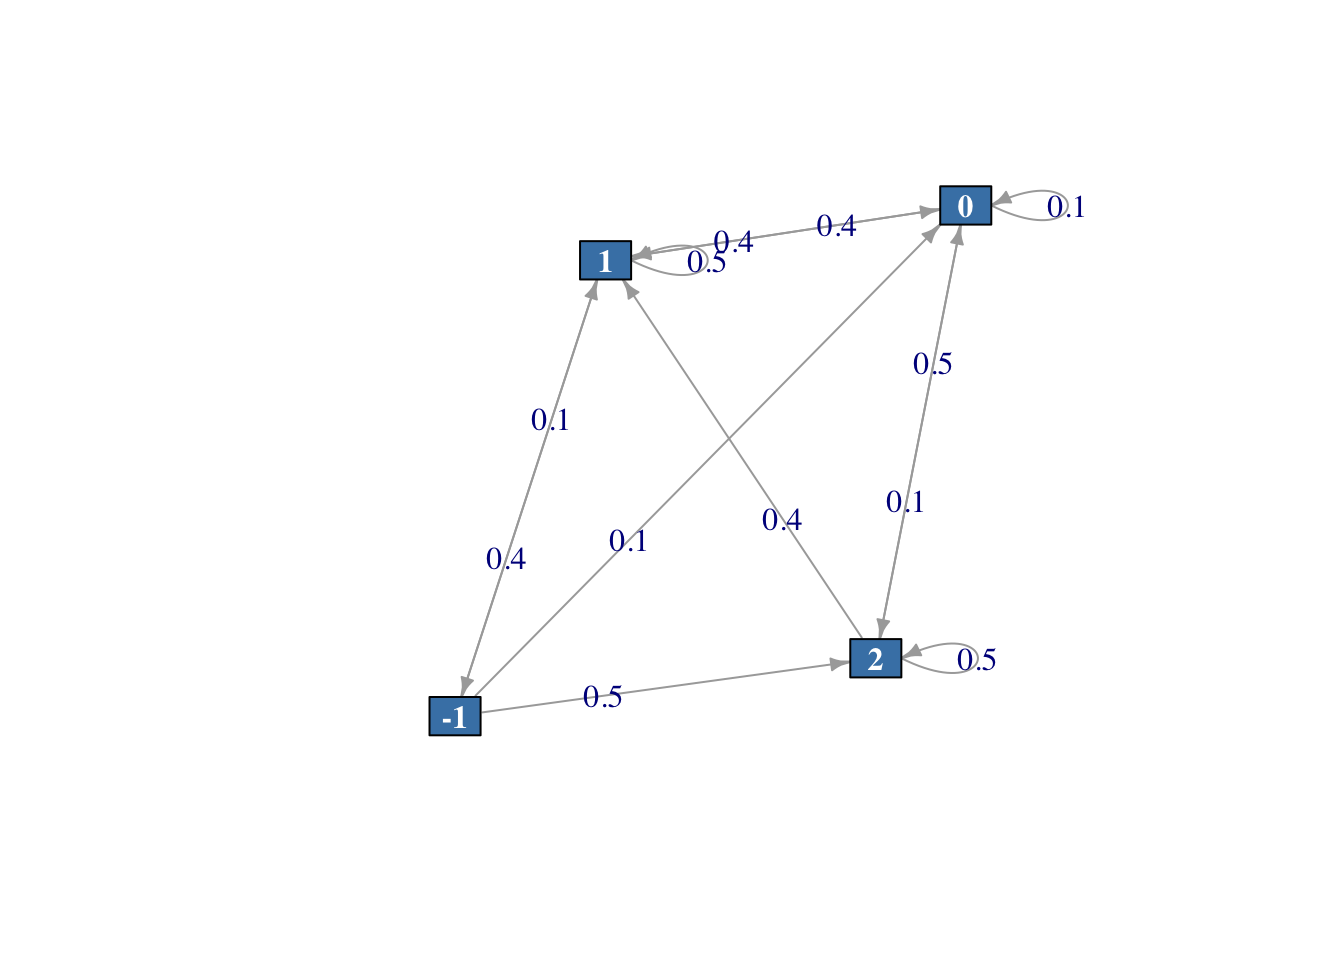
\includegraphics[width=0.95\linewidth]{02-CMTD_files/figure-latex/03-019-3-1} 

}

\caption{Diagrama del sistema del problema de inventario.}\label{fig:03-019-3}
\end{figure}

\hypertarget{CaracCMTD}{%
\section{Caracterización de una CMTD}\label{CaracCMTD}}

En esta sección estudiamos las principales características de una \(CMTD\) a través de la comunicación entre los diferentes estados de proceso, el número de visitas y los tiempos de ocupación de cada estado, los tiempos a la primera visita, partiendo de un estado, e introducimos la utilización de costes para la evaluación de los sistemas.

En todas las definiciones que presentamos a continuación asumimos que tenemos una \(CMTD\) \(\{X_n, n \in \mathbb{N}\}\) con espacio de estados \(S\) y matriz de transición de un paso \(P\).

\hypertarget{comunicaciuxf3n-entre-estados}{%
\subsection{Comunicación entre estados}\label{comunicaciuxf3n-entre-estados}}

Comenzamos caracterizando los estados de una cadena en función de sus probabilidades de transición.

\begin{yellowbox}

\begin{definition}
Dados dos estados \(i, j\) de \(S\), se dice que el estado \(j\) es \textbf{accesible} desde el estado \(i\) si existe una transición \(n\) tal que \(p_{ij}(n) > 0\).

Que el estado \(j\) sea accesible desde \(i\) se denota habitualmente como \(i \rightarrow j\).
\end{definition}

\end{yellowbox}

\begin{yellowbox}

\begin{definition}
Dados dos estados \(i, j\) de \(S\), se dice que son \textbf{comunicantes} si \(i\) es accesible desde \(j\), y \(j\) es accesible desde \(i\), es decir, existen \(n_1\) y \(n_2\) tal que \(p_{ij}(n_1) > 0\) y \(p_{ji}(n_2) > 0.\)

Que los estados \(i, j\) sean comunicantes se denota habitualmente como \(i \leftrightarrow j\).
\end{definition}

\end{yellowbox}

\begin{yellowbox}

\begin{definition}
Un subconjunto de estados \(S_j \subset S\) se denomina \textbf{clase comunicante} del estado \(j\) si todos los estados de ese subconjunto son comunicantes con \(j\).

\[S_j \subset S \text{ es clase comunicante de } j \text{ si } \quad i \leftrightarrow j, \qquad \forall i \in S_j.\]
\end{definition}

\end{yellowbox}

\begin{yellowbox}

\begin{definition}
Un estado \(i \in S\) se denomina \textbf{estado sin retorno} cuando no es viable volver a dicho estado tras partir de él, esto es, para \(n \geq 1\), \(p_{ii}(n) = 0.\)
\end{definition}

\end{yellowbox}

\begin{yellowbox}

\begin{definition}
Un conjunto de estados \(C \subset S\) se denomina \textbf{cerrado} cuando no es posible pasar de un estado de \(C\) a otro que no esté en \(C\), esto es,

\[\forall i \in C, \quad \forall j \notin C \quad \Rightarrow \quad p_{ij}(n) = 0, \quad n\geq 1\]
o lo que es lo mismo,

\[ \sum_{j \in C} p_{ij}=1, \quad \forall i \in C.\]

Esto implica que cuando accedamos a un conjunto cerrado, será imposible salir de él y sólo será factible moverse dentro de él.

Si el conjunto cerrado está compuesto por un único estado \(i\) diremos que ese estado \(i\) es \textbf{absorbente}. Eso implica que si se llega a dicho estado, el proceso se queda estancado en él y ya no es posible moverse a otro estado.
\end{definition}

\end{yellowbox}

\begin{yellowbox}

\begin{definition}
Una \(CMTD\) es \textbf{irreducible} cuando todos sus estados están comunicados entre sí, esto es, para cualquier \(i,j \in S\) existe algún instante de tiempo \(n \geq 0\) tal que \(Pr(X_n=j|X_0=i)>0\). Un conjunto de estados en S se dice irreducible cuando no contiene ningún subconjunto cerrado. Si la \(CMTD\) no es irreducible, se llama \textbf{reducible}.

Todos los estados dentro de un conjunto irreducible son del mismo tipo.
\end{definition}

\end{yellowbox}

\begin{whitebox}
Para caracterizar una CMTD mediante la librería \texttt{markovchain} es útil usar la función \texttt{summary(object)} donde `object' identifica el proceso a estudiar.

\end{whitebox}

\begin{example}
\protect\hypertarget{exm:summary-markovchain}{}\label{exm:summary-markovchain}Queremos caracterizar el proceso presentado en el Ejemplo \ref{exm:diagramCMTD}. Cargamos los datos y ejecutamos la sintaxis a continuación.

\begin{Shaded}
\begin{Highlighting}[]
\CommentTok{\# Caracterización}
\FunctionTok{summary}\NormalTok{(proceso)}
\end{Highlighting}
\end{Shaded}

\begin{verbatim}
## Unnamed Markov chain  Markov chain that is composed by: 
## Closed classes: 
## a b c 
## Recurrent classes: 
## {a,b,c}
## Transient classes: 
## NONE 
## The Markov chain is irreducible 
## The absorbing states are: NONE
\end{verbatim}

A la vista del resultado, concluimos que este proceso es cerrado (todo su espacio de estados es cerrado). Todos sus estados son recurrentes y no tiene estados transitorios (estos conceptos los veremos más adelante). No tiene estados absorbentes y la cadena de Markov es irreducible (todos sus estados están comunicados).
\end{example}

\begin{bluebox}
\textbf{PRACTICA} Caracterizar los procesos: \protect\hyperlink{fiabilidad}{Fiabilidad de máquinas},\protect\hyperlink{meteo}{Metereología}, \protect\hyperlink{inventario}{Problema de inventario}, \protect\hyperlink{planificacion}{Planificación de mano de obra}, \protect\hyperlink{mercadovalores}{Mercado de valores} e \protect\hyperlink{inventario2}{Inventario con desabastecimiento}.

\end{bluebox}

\begin{example}

Veamos ahora cómo utilizar la simulación para responder a diferentes preguntas de interés. En concreto, para el ejemplo en la sección \protect\hyperlink{inventario2}{Inventario con desabastecimiento} (recordemos que se trataba de un almacén que se reabastecía cuando el inventario quedaba por debajo o igual a un nivel mínimo de almacenaje, \(A=0\), y con una política de reabastecimiento que dependía del nivel de almacenaje máximo \(B=2\)), planteamos estas preguntas:

\begin{enumerate}
\def\labelenumi{\arabic{enumi}.}
\item
  Durante las próximas 20 semanas, ¿en cuántas de ellas será preciso reabastecerse?
\item
  Durante las próximas 20 semanas, ¿cuál es la proporción de semanas en que la demanda no ha sido satisfecha (por rebasar el stock)?
\end{enumerate}

\end{example}

Para responder estas preguntas hay que considerar el proceso \(\{X_n, n \geq 0\}\) y la variable \(Y_n\) que identifica la demanda en la semana \(n\). Planteamos el siguiente algoritmo de simulación.

\begin{silverbox}

\textbf{Algoritmo para simulación de inventario}

\begin{itemize}
\tightlist
\item
  Paso 1. Fijar el número de transiciones del proceso, \(n\), e inicializar \(X_0 = 2\) (máximo almacenaje).
\end{itemize}

Repetir pasos 2 y 3 hasta alcanzar el número de transiciones deseadas.

\begin{itemize}
\item
  Paso 2. Generar \(Y_i\) con el método de la transformada inversa.
\item
  Paso 3. Actualizar el valor \(X_i\) y reabastecer si fuera necesario.
\item
  Paso 4. Devolver la secuencia \(\{X_i, Y_i; i=1,\ldots,n\}\) para estudiar la evolución del sistema y la demanda.
\end{itemize}

\end{silverbox}

Desarrollemos pues, el algoritmo.

\begin{Shaded}
\begin{Highlighting}[]
\CommentTok{\# Inicialización}
\FunctionTok{set.seed}\NormalTok{(}\DecValTok{12}\NormalTok{)}
\NormalTok{tiempo }\OtherTok{\textless{}{-}} \DecValTok{21} \CommentTok{\# valor inicial y 20 transiciones}
\NormalTok{invent }\OtherTok{\textless{}{-}} \FunctionTok{c}\NormalTok{()  }\CommentTok{\# vector con los valores de inventario}
\NormalTok{demanda }\OtherTok{\textless{}{-}} \FunctionTok{c}\NormalTok{() }\CommentTok{\# vector con los valores de demanda}
\NormalTok{A }\OtherTok{\textless{}{-}} \DecValTok{0}
\NormalTok{B }\OtherTok{\textless{}{-}} \DecValTok{2}
\DocumentationTok{\#\#\#\#\# Configuración metodo transformada inversa \#\#\#\#\#\#}
\CommentTok{\# datos uniformes}
\NormalTok{unif }\OtherTok{\textless{}{-}} \FunctionTok{runif}\NormalTok{(tiempo}\DecValTok{{-}1}\NormalTok{)}
\CommentTok{\# Valores posibles para la demanda}
\NormalTok{valores }\OtherTok{\textless{}{-}} \FunctionTok{c}\NormalTok{(}\DecValTok{0}\NormalTok{, }\DecValTok{1}\NormalTok{, }\DecValTok{2}\NormalTok{)}
\CommentTok{\# Probabilidades para la demanda}
\NormalTok{prob }\OtherTok{\textless{}{-}} \FunctionTok{c}\NormalTok{(}\FloatTok{0.5}\NormalTok{, }\FloatTok{0.4}\NormalTok{, }\FloatTok{0.1}\NormalTok{)}
\NormalTok{probacum }\OtherTok{\textless{}{-}} \FunctionTok{cumsum}\NormalTok{(prob)  }\CommentTok{\# probabilidades acumuladas}
\CommentTok{\# valor inicial del proceso}
\NormalTok{invent[}\DecValTok{1}\NormalTok{] }\OtherTok{\textless{}{-}} \DecValTok{2}
\NormalTok{demanda[}\DecValTok{1}\NormalTok{] }\OtherTok{\textless{}{-}} \DecValTok{0}
\NormalTok{i}\OtherTok{\textless{}{-}}\DecValTok{2}
\ControlFlowTok{while}\NormalTok{ (i }\SpecialCharTok{\textless{}=}\NormalTok{ tiempo)}
\NormalTok{\{}
  \CommentTok{\# simulamos demanda}
\NormalTok{  demanda[i] }\OtherTok{\textless{}{-}}\NormalTok{ valores[}\FunctionTok{min}\NormalTok{(}\FunctionTok{which}\NormalTok{(unif[i}\DecValTok{{-}1}\NormalTok{] }\SpecialCharTok{\textless{}=}\NormalTok{ probacum))] }
  \CommentTok{\# Actualizamos inventario}
  \FunctionTok{ifelse}\NormalTok{(invent[i}\DecValTok{{-}1}\NormalTok{] }\SpecialCharTok{\textless{}=}\NormalTok{ A, }
\NormalTok{         invent[i] }\OtherTok{\textless{}{-}}\NormalTok{ B }\SpecialCharTok{{-}}\NormalTok{ demanda[i], }
\NormalTok{         invent[i] }\OtherTok{\textless{}{-}}\NormalTok{ invent[i}\DecValTok{{-}1}\NormalTok{]}\SpecialCharTok{{-}}\NormalTok{demanda[i])}
  \CommentTok{\# iteración siguiente}
\NormalTok{  i}\OtherTok{\textless{}{-}}\NormalTok{i}\SpecialCharTok{+}\DecValTok{1}
\NormalTok{\}}
\CommentTok{\# Devolvemos la secuencia de estados }
\NormalTok{inventario2.sim}\OtherTok{=}\FunctionTok{data.frame}\NormalTok{(invent,demanda)}
\FunctionTok{head}\NormalTok{(inventario2.sim)}
\end{Highlighting}
\end{Shaded}

\begin{verbatim}
##   invent demanda
## 1      2       0
## 2      2       0
## 3      1       1
## 4     -1       2
## 5      2       0
## 6      2       0
\end{verbatim}

La estimación del número de semanas que hay que reabastecerse viene dada por el número de simulaciones en las que el nivel de inventario es menor o igual al nivel mínimo de almacenamiento, \(invent=X\leq 0\), es decir

\begin{Shaded}
\begin{Highlighting}[]
\FunctionTok{sum}\NormalTok{(inventario2.sim}\SpecialCharTok{$}\NormalTok{invent }\SpecialCharTok{\textless{}=}\NormalTok{ A)}
\end{Highlighting}
\end{Shaded}

\begin{verbatim}
## [1] 3
\end{verbatim}

La proporción de semanas en que la demanda no ha sido satisfecha (por rebasar el stock) corresponde a aquellas en las que la demanda ha superado al inventario,

\begin{Shaded}
\begin{Highlighting}[]
\FunctionTok{mean}\NormalTok{(inventario2.sim}\SpecialCharTok{$}\NormalTok{invent }\SpecialCharTok{\textless{}}\NormalTok{inventario2.sim}\SpecialCharTok{$}\NormalTok{demanda)}
\end{Highlighting}
\end{Shaded}

\begin{verbatim}
## [1] 0.1428571
\end{verbatim}

\hypertarget{tiemposocupa-sec}{%
\subsection{Tiempos de ocupación}\label{tiemposocupa-sec}}

\begin{yellowbox}

\begin{definition}

Sea \(\{X_n, n \geq 0\}\) una \(CMTD\) homogénea con espacio de estados \(S = \{1, 2,...,N\}\), matriz de probabilidades de transición de una paso \(P\), y distribución inicial \(p(0)\). Consideramos la variable aleatoria \(N_j(n)\) como el \textbf{número de visitas al estado \(j\) en \(n\) transiciones} y definimos

\[m_{ij}(n) = E[N_j(n)|X_0 = i]\]
como el \textbf{número esperado de visitas} o \textbf{tiempo de ocupación del estado \(j\) hasta el instante \(n\), partiendo del estado \(i\)}.

A partir de las cantidades \(m_{ij}(n)\) se puede definir la \textbf{matriz de tiempos de ocupación hasta un instante} \(n\), \(M(n)=(m_{ij}(n))_{ij}\), que se puede calcular a partir de la matriz de transición \(P\) como:

\begin{equation}
M(n) = \sum_{r=0}^n P^r
\label{eq:tposocupa}
\end{equation}

\end{definition}

\end{yellowbox}

\begin{yellowbox}

\begin{definition}
Un estado \(i\) se dice que es \textbf{recurrente} si es continuamente revisitado a lo largo de la vida de la cadena, esto es, el número esperado de visitas al estado \(i\) a lo largo de la vida del proceso es infinito, \(m_{ii}=E(N_i|X_0=i)=\infty\). En otro caso, cuando sólo se accede un número finito de veces, se dice que es \textbf{transitorio}. Un estado transitorio sólo será accesible durante un cierto periodo de tiempo, tras el cual dicho estado ya no será revisitado nunca más.
\end{definition}

\end{yellowbox}

\begin{example}
Volvemos sobre el Ejemplo \ref{exm:diagramCMTD} para calcular los tiempos de ocupación durante un periodo continuado de 10 transiciones. Para ello utilizamos la Ecuación \eqref{eq:tposocupa} con \(n=10\).

\begin{Shaded}
\begin{Highlighting}[]
\DocumentationTok{\#\# Simulación de los tiempos de ocupación (número de visitas a un estado)}
\CommentTok{\# Número de estados del proceso}
\NormalTok{nestat }\OtherTok{\textless{}{-}} \FunctionTok{dim}\NormalTok{(proceso)}
\CommentTok{\# Estados}
\NormalTok{nombres}\OtherTok{\textless{}{-}} \FunctionTok{names}\NormalTok{(proceso)}
\CommentTok{\# Generamos la matriz de ocupaciones}
\CommentTok{\# el primer elemento es la matriz identidad: p\^{}0}
\NormalTok{mocupa }\OtherTok{\textless{}{-}} \FunctionTok{diag}\NormalTok{(nestat)}
  \FunctionTok{dimnames}\NormalTok{(mocupa) }\OtherTok{\textless{}{-}} \FunctionTok{list}\NormalTok{(nombres, nombres)}
\CommentTok{\# Bucle de cálculo de los tiempos de ocupación}
\NormalTok{P}\OtherTok{=}\NormalTok{proceso[}\DecValTok{1}\SpecialCharTok{:}\NormalTok{nestat,}\DecValTok{1}\SpecialCharTok{:}\NormalTok{nestat] }\CommentTok{\# matriz de transición}
\ControlFlowTok{for}\NormalTok{ (i }\ControlFlowTok{in} \DecValTok{1}\SpecialCharTok{:}\DecValTok{10}\NormalTok{)}
\NormalTok{\{}
\NormalTok{   mocupa }\OtherTok{\textless{}{-}}\NormalTok{ mocupa }\SpecialCharTok{+} \FunctionTok{ptran.n}\NormalTok{(P,i)}
\NormalTok{\}}
\NormalTok{mocupa}
\end{Highlighting}
\end{Shaded}

\begin{verbatim}
##          a        b        c
## a 4.531739 1.248415 5.219845
## b 3.555292 1.955489 5.489220
## c 3.858338 1.046384 6.095278
\end{verbatim}

Podemos ver cómo el número esperado de visitas al estado \(c\) partiendo del estado \(b\) en las próximas 10 transiciones es casi de 7 (6.86). Sin embargo, si partimos del estado \(b\), en 10 transiciones sólo esperamos volver a dicho estado 1 vez.
\end{example}

\begin{whitebox}

Definamos una función para obtener la matriz de tiempos de ocupación (o número esperado de visitas) durante un periodo de duración de \(n\) unidades de tiempo.

\begin{Shaded}
\begin{Highlighting}[]
\CommentTok{\# Función para calcular los tiempos de ocupación en un periodo [0,n]}
\NormalTok{mocupa.proceso }\OtherTok{\textless{}{-}} \ControlFlowTok{function}\NormalTok{(proceso, n)}
\NormalTok{\{}
  \CommentTok{\# Número de estados del proceso}
\NormalTok{  nestat }\OtherTok{\textless{}{-}} \FunctionTok{dim}\NormalTok{(proceso)}
  \CommentTok{\# Estados}
\NormalTok{  nombres}\OtherTok{\textless{}{-}} \FunctionTok{names}\NormalTok{(proceso)}
  \CommentTok{\# Generamos la matriz de ocupaciones}
\NormalTok{  mocupa }\OtherTok{\textless{}{-}} \FunctionTok{diag}\NormalTok{(nestat)}
  \FunctionTok{dimnames}\NormalTok{(mocupa) }\OtherTok{\textless{}{-}} \FunctionTok{list}\NormalTok{(nombres, nombres)}
\CommentTok{\#  mocupa \textless{}{-} matrix(rep(0, nestat*nestat),}
\CommentTok{\#                 nrow = nestat, dimnames = list(nombres, nombres))}
  \CommentTok{\# Bucle de cálculo de los tiempos de ocupación}
\NormalTok{  P}\OtherTok{=}\NormalTok{proceso[}\DecValTok{1}\SpecialCharTok{:}\NormalTok{nestat,}\DecValTok{1}\SpecialCharTok{:}\NormalTok{nestat]}
  \ControlFlowTok{for}\NormalTok{ (i }\ControlFlowTok{in} \DecValTok{1}\SpecialCharTok{:}\NormalTok{n)}
\NormalTok{   mocupa }\OtherTok{\textless{}{-}}\NormalTok{ mocupa }\SpecialCharTok{+} \FunctionTok{ptran.n}\NormalTok{(P,i)}
  
  \FunctionTok{return}\NormalTok{(mocupa)}
\NormalTok{\}}
\end{Highlighting}
\end{Shaded}

\end{whitebox}

\begin{bluebox}
\textbf{PRACTICA} Obtener y caracterizar la matriz del número esperado de visitas en 20 transiciones para los procesos: \protect\hyperlink{fiabilidad}{Fiabilidad de máquinas},\protect\hyperlink{meteo}{Metereología}, \protect\hyperlink{inventario}{Problema de inventario}, \protect\hyperlink{planificacion}{Planificación de mano de obra} y \protect\hyperlink{mercadovalores}{Mercado de valores}.

\end{bluebox}

\hypertarget{anuxe1lisis-de-costes}{%
\subsection{Análisis de costes}\label{anuxe1lisis-de-costes}}

Una aplicación muy habitual de los tiempos de ocupación es directa en los denominados \textbf{modelos de costes}, que describimos brevemente, y que pueden estar vinculados en situaciones específicas a costes, pero también a beneficios, pérdidas, etc..

Sea \(X_n\) el estado del sistema en el tiempo \(n\). Asumimos que \(\{X_n, n \geq 0 \}\) es una \(CMTD\) con espacio de estados \(S =\{1, 2,...,N\}\), matriz de transición \(P\), y matriz de tiempos de ocupación \(M(n)\).

En esta situación, hablamos de que cada visita a cierto estado \(i\) tiene un coste aleatorio asociado \(C(i)\), y el coste esperado por cada visita al estado \(i\) viene dado por \(c(i) = E[C(i)]\). Definimos la matriz de costes esperados asociados a los estados, como \(\mathbf{c}\), de dimensión \(N\times 1\), como:

\[\mathbf{c}' = (c(1),c(2),\ldots,c(N))\]

Así mismo, hablamos del coste \(C(X_r)\) en el que incurre el sistema en un instante concreto \(r\), y \(\sum_{r=0}^n C(X_r)\) el coste acumulado desde el inicio del proceso hasta llegar al instante \(n\). Entonces el \textbf{coste esperado total (CET)} asociado al funcionamiento del sistema hasta llegar al instante \(n\) se calculará como

\[CET=E\left[\sum_{r=0}^n C(X_r)\right]\]

Definimos el coste esperado total hasta el instante \(n\) partiendo del estado \(i\), \(g(i,n)\), como:

\[g(i,n) = E\left[\sum_{r=0}^n C(X_r)| X_0 = i \right]\]

y construimos la matriz de \textbf{costes totales sobre un horizonte finito (CTHF) hasta el instante \(n\)}, \(\mathbf{g}(n)\), de dimensión \(N \times 1\), a través de estos costes esperados partiendo de cualesquier estado \(i \in S\), como

\[\mathbf{g}(n)' = (g(1,n),g(2,n),\ldots,g(N,n))\]

\begin{yellowbox}

\begin{definition}

Si vinculado al funcionamiento de un sistema CMTD queremos calcular el \textbf{coste esperado total sobre un horizonte finito hasta un instante \(n\)}, (CTHF), basta multiplicar la matriz de tiempos de ocupación hasta el instante \(n\), \(M(n)\), por la matriz de costes esperados asociados a los estados del sistema, \(\mathbf{c}\), esto es, resolver la Ecuación \eqref{eq:CTHF}.

\begin{equation}
\mathbf{g}(n) = M(n) \cdot \mathbf{c}
\label{eq:CTHF}
\end{equation}

\end{definition}

\end{yellowbox}

\begin{example}
Volvamos al proceso de inventario presentado en el \protect\hyperlink{inventario}{Problema de inventario} con espacio de estados \(\{2,3,4,5\}\). Supongamos que la empresa compra PCs por 1500 euros y los vende por 1750 euros. Además el coste de almacenamiento semanal es de 50 euros por cada unidad que está en la tienda al inicio de una semana. Queremos calcular los ingresos netos que la tienda espera obtener durante las próximas 10 semanas, suponiendo que comienza con cinco PCs en stock al inicio del periodo.
\end{example}

En esta situación, estamos interesados en los ingresos, por lo que definimos \(c(i)\) como los ingresos netos que se obtienen en una semana cualquiera en la que hay \(i\) PCs al principio de la semana. Sabemos que los costes de almacenamiento de \(i\) PCs es \(50i\). Las ganancias provendrán de los PCs que se hayan vendido. Si \(D_n\) es la demanda durante una semana cualquiera \(n\), el número esperado de PCs vendidos durante esa semana será \(E[min(i, D_n)]\). Así, los ingresos netos previstos para una semana cualquiera \(n\) en la que se tienen \(i\) PCs almacenados al inicio, \(c(i)\), provendrán de los ingresos por ventas menos los gastos de almacenaje, esto es,

\[c(i) = (1750-1500)E[min(i, D_n)] -50i, \quad 2 \leq i \leq 5\]

Necesitamos pues, obtener el valor de \(E[min(i, D_n)]\), para cada valor de \(i\). Veamos cómo hacerlo, tanto de forma teórica como mediante simulación. Denotemos por \(Z_{i,n} = min(i, D_n),\) para \(i=2, 3, 4, 5\) de forma que:

\begin{equation*}
Z_{i,n} =  
\begin{cases}
i & \text{ si } i <D_n \\
D_n & \text{ si } i \geq  D_n 
\end{cases}
\end{equation*}

de esta forma tenemos que su valor esperado vendrá dado por:

\[E[Z_{i,n}] = i \cdot Pr[i < D_n] + \sum_{d=0}^{i} d \cdot Pr(D_n=d).\]

Recordando que \(D_n\sim Pois(3)\) en el ejemplo original, para \(i=2\) la expresión anterior da lugar a:

\begin{eqnarray*}
E[Z_{2,n}] &= 2 \cdot Pr[D_n > 2] + 0 \cdot Pr[D_n = 0] + 1 \cdot Pr[D_n =1] +2 \cdot Pr(D_n=2) \\
&= 2 \cdot (1-Pr(D_n \leq 2)) + 1 \cdot Pr[D_n =1] + 2 \cdot Pr(D_n=2) \\
&= 2 \cdot 0.5768 +0.1494 +2 \cdot 0.2240 = 1.751
\end{eqnarray*}

de donde calculamos los ingresos \(c(2)\) con la ecuación anterior.
\[c(2) =  250 \cdot 1.751 -50 \cdot 2 = 337.75\]
Hacemos fácilmente los cálculos para todos los estados:

\begin{Shaded}
\begin{Highlighting}[]
\NormalTok{estados}\OtherTok{=}\DecValTok{2}\SpecialCharTok{:}\DecValTok{5}
\NormalTok{lambda}\OtherTok{=}\DecValTok{3}   \CommentTok{\# Poisson para la demanda}
\CommentTok{\# número esperado de ventas}
\NormalTok{ez}\OtherTok{=}\FunctionTok{c}\NormalTok{()}
\ControlFlowTok{for}\NormalTok{(i }\ControlFlowTok{in}\NormalTok{ estados)\{}
\NormalTok{ez[i}\DecValTok{{-}1}\NormalTok{]}\OtherTok{=}\NormalTok{i}\SpecialCharTok{*}\NormalTok{(}\DecValTok{1}\SpecialCharTok{{-}}\FunctionTok{ppois}\NormalTok{(i,lambda))}\SpecialCharTok{+}\FunctionTok{sum}\NormalTok{((}\DecValTok{0}\SpecialCharTok{:}\NormalTok{i)}\SpecialCharTok{*}\FunctionTok{dpois}\NormalTok{(}\DecValTok{0}\SpecialCharTok{:}\NormalTok{i,lambda))}
\NormalTok{\}}
\NormalTok{ingresos}\OtherTok{=}\DecValTok{250}\SpecialCharTok{*}\NormalTok{ez}\DecValTok{{-}50}\SpecialCharTok{*}\NormalTok{estados;ingresos}
\end{Highlighting}
\end{Shaded}

\begin{verbatim}
## [1] 337.7662 431.9686 470.1607 466.3449
\end{verbatim}

Y obtenemos

\[\mathbf{c} = 
\begin{pmatrix}
337.75 \\
431.95 \\
470.15 \\
466.23 
\end{pmatrix}\]

Con esta matriz y la matriz de ocupación hasta el instante \(n=10\) podemos calcular los ingresos netos totales esperados durante las próximas \(n=10\) semanas, sea cual sea el estado inicial del sistema:

\[g(10)=M(10) \cdot c\]
que calculamos a continuación:

\begin{Shaded}
\begin{Highlighting}[]
\NormalTok{c}\OtherTok{=}\FunctionTok{matrix}\NormalTok{(}\FunctionTok{round}\NormalTok{(ingresos,}\DecValTok{2}\NormalTok{), }\AttributeTok{ncol=}\DecValTok{1}\NormalTok{)}
\NormalTok{M10}\OtherTok{=}\FunctionTok{mocupa.proceso}\NormalTok{(inventario,}\DecValTok{10}\NormalTok{)}
\NormalTok{g}\OtherTok{=}\NormalTok{M10 }\SpecialCharTok{\%*\%}\NormalTok{ c}
\NormalTok{g}
\end{Highlighting}
\end{Shaded}

\begin{verbatim}
##           [,1]
## 2 PCs 4736.876
## 3 PCs 4819.392
## 4 PCs 4847.637
## 5 PCs 4842.589
\end{verbatim}

y que nos permite extraer los ingresos netos totales esperados asumiendo que el periodo inicia con \(i=5\) PCs en tienda, esto es, como \$g(5,10)=\$4842.59 euros.

Los valores de \(c\) se pueden aproximar mediante simulación sin necesidad de calcularlos de forma teórica. A continuación se presenta el código necesario para realizar la simulación. Concretamente definimos una función que depende del valor del estado inicial \(i\).

\begin{Shaded}
\begin{Highlighting}[]
\CommentTok{\# simulador del valor esperado del número esperado de ventas}
\NormalTok{c.sim }\OtherTok{\textless{}{-}} \ControlFlowTok{function}\NormalTok{(estado, nsim)}
\NormalTok{\{}
  \CommentTok{\# estado: estado inicial del sistema}
  \CommentTok{\# nsim: nº simulaciones para la aproximación}
  
  \CommentTok{\# Simulamos valores del mínimo entre i y D\_n}
\NormalTok{  datos }\OtherTok{\textless{}{-}} \FunctionTok{data.frame}\NormalTok{(}\AttributeTok{rsim =} \FunctionTok{rpois}\NormalTok{(nsim, }\DecValTok{3}\NormalTok{), rdos }\OtherTok{\textless{}{-}} \FunctionTok{rep}\NormalTok{(estado, nsim))}
\NormalTok{  minimo }\OtherTok{\textless{}{-}}\FunctionTok{apply}\NormalTok{(datos, }\DecValTok{1}\NormalTok{ ,min) }\CommentTok{\# Mínimo por filas}
  \CommentTok{\# Valor esperado min(i,D\_n)}
\NormalTok{  esperanza }\OtherTok{\textless{}{-}} \FunctionTok{mean}\NormalTok{(minimo)}
  \CommentTok{\# coste}
\NormalTok{  coste }\OtherTok{\textless{}{-}} \FunctionTok{round}\NormalTok{(}\SpecialCharTok{{-}}\DecValTok{50}\SpecialCharTok{*}\NormalTok{estado}\SpecialCharTok{+}\DecValTok{250}\SpecialCharTok{*}\NormalTok{esperanza, }\DecValTok{2}\NormalTok{)}
  \FunctionTok{return}\NormalTok{(coste)}
\NormalTok{\}}
\end{Highlighting}
\end{Shaded}

Aproximamos pues por simulación, los valores de la matriz \(c\) con \(nsim=1.000.000\) simulaciones

\begin{Shaded}
\begin{Highlighting}[]
\NormalTok{nsim }\OtherTok{\textless{}{-}} \DecValTok{1000000}
\FunctionTok{set.seed}\NormalTok{(}\DecValTok{12}\NormalTok{)}
\NormalTok{c.s}\OtherTok{=}\FunctionTok{matrix}\NormalTok{(}\FunctionTok{c}\NormalTok{(}\FunctionTok{c.sim}\NormalTok{(}\DecValTok{2}\NormalTok{, nsim),}\FunctionTok{c.sim}\NormalTok{(}\DecValTok{3}\NormalTok{, nsim),}
      \FunctionTok{c.sim}\NormalTok{(}\DecValTok{4}\NormalTok{, nsim),}\FunctionTok{c.sim}\NormalTok{(}\DecValTok{5}\NormalTok{, nsim)),}\AttributeTok{ncol=}\DecValTok{1}\NormalTok{)}
\NormalTok{c.s}
\end{Highlighting}
\end{Shaded}

\begin{verbatim}
##        [,1]
## [1,] 337.66
## [2,] 431.61
## [3,] 470.28
## [4,] 466.69
\end{verbatim}

Como se puede ver, la simulación funciona bastante bien para aproximar el vector \(c\); resolvamos pues los cálculos de \(g(5,10)\) con estos valores, que de nuevo aproximarán las cantidades que buscamos.

\begin{Shaded}
\begin{Highlighting}[]
\CommentTok{\# matriz M}
\NormalTok{Mmat }\OtherTok{\textless{}{-}} \FunctionTok{mocupa.proceso}\NormalTok{(inventario, }\DecValTok{10}\NormalTok{)}
\CommentTok{\# vector g}
\NormalTok{beneficio }\OtherTok{\textless{}{-}}\NormalTok{ Mmat}\SpecialCharTok{\%*\%}\NormalTok{c.s}
\NormalTok{beneficio}
\end{Highlighting}
\end{Shaded}

\begin{verbatim}
##           [,1]
## 2 PCs 4738.291
## 3 PCs 4820.502
## 4 PCs 4849.143
## 5 PCs 4844.266
\end{verbatim}

Mientras que teóricamente obteníamos unos ingresos esperados de 4842.59€, con la simulación obtenemos una aproximación de 4844.27€.

\hypertarget{tiempos-de-primer-paso}{%
\subsection{Tiempos de primer paso}\label{tiempos-de-primer-paso}}

\begin{yellowbox}

\begin{definition}
Sea \(\{X_n, n \geq 0\}\) una \(CMTD\) homogénea con espacio de estados \(S = \{1, 2,...,N\}\). Se define el \textbf{tiempo de primer paso} o \textbf{tiempo de primera visita} al estado \(j\) partiendo del estado \(i\), \(T_{ij}\), como el mínimo número de transiciones necesarias para alcanzar el estado \(j\) partiendo del estado inicial \(i\), es decir:

\[T_{ij} = \underset{n}{min}\{n > 0, X_n = j | X_0 = i\}\]

En ocasiones interesará sin embargo el tiempo de primer paso de un estado a un conjunto de estados \(A\):

\[T_{iA} = \underset{n}{min}\{n > 0, X_n \in A | X_0 = i\}.\]
\end{definition}

\end{yellowbox}

\begin{whitebox}
Para obtener los tiempos esperados de recurrencia \(f=(f_{11},...,f_{NN})\) para el espacio de estados \(S=\{1,...,N\}\), utilizamos la función \texttt{meanRecurrenceTime(proceso)} de la librería \texttt{markovchain}.

Para obtener los tiempos esperados de primer paso por un estado \(j\) desde cualquier estado de \(S\), podemos utilizar la función \texttt{meanFirstPassageTime(proceso,destination=j)} de la librería \texttt{markovchain}.
Si queremos calcular la matriz de tiempos esperados para llegar a cualquier estado desde cualquier estado, basta utilizar \texttt{meanFirstPassageTime(proceso)}.

\end{whitebox}

En caso de que no podamos utilizar la función \texttt{meanFirstPassageTime} para el cálculo del tiempo esperado de primer paso, podemos utilizar la propiedad que pasamos a describir.

\begin{yellowbox}

\begin{definition}
Sea \(\{X_n, n \geq 0\}\) una \(CMTD\) con espacio de estados \(S = \{1, 2,...,N\}\). Si estamos interesados en obtener el tiempo esperado de primer paso para el estado \(j\) desde cualquier estado \(i\), dado por:

\[v_{ij} = E(T_{ij}), \quad \text{ con } T_{ij} = \underset{n}{min}\{n > 0, X_n = j | X_0 = i\}\]

y construimos la matriz de dimensión \((N-1) \times 1\) \(\mathbf{v_j'}=(v_{1j},...,v_{j-1,j},v_{j+1,j},...,v_{Nj})\)\\
basta con resolver el sistema:

\begin{equation}
[\mathbf{I} - P_{-j}]\mathbf{v_j} = \mathbf{1}
\label{eq:primerpaso-ecu}
\end{equation}

donde

\begin{itemize}
\tightlist
\item
  \(P_{-j}\) es la matriz de transición eliminando la fila y columna del estado \(j\),
\item
  \(\mathbf{1}\) es un vector de unos, de dimensión \(N-1\),
\item
  \(\mathbf{I}\) es una matriz diagonal de las mismas dimensiones que \(P_{-N}\).
\end{itemize}

Esta ecuación se puede generalizar para obtener los tiempos esperados de primer paso desde un estado \(i\) hasta cualquier subconjunto de estados \(S_c \subset S\).
\end{definition}

\end{yellowbox}

\begin{whitebox}

\textbf{Función para obtener los tiempos esperados de primer paso}

Como alternativa a la función definida en \texttt{markovchain}, programamos a continuación una función genérica para poder obtener los tiempos esperados de primer paso, dependiente de dos parámetros:

\begin{itemize}
\tightlist
\item
  proceso: \(CMTD\) que describe el sistema a estudio
\item
  estado: estado o conjunto de estados que se desean alcanzar, partiendo desde cualquier estado inicial que no está en este conjunto.
\end{itemize}

\begin{Shaded}
\begin{Highlighting}[]
\CommentTok{\# Función para obtener el tiempo esperado de primer paso por "estado"}
\CommentTok{\# (equivalente a meanFirstPassageTime de markovchain)}
\NormalTok{tiempo.pp }\OtherTok{\textless{}{-}} \ControlFlowTok{function}\NormalTok{(proceso, estado)}
\NormalTok{\{}
  \CommentTok{\# estados del proceso}
\NormalTok{  estados }\OtherTok{\textless{}{-}} \FunctionTok{states}\NormalTok{(proceso)}
\NormalTok{  numestados }\OtherTok{\textless{}{-}} \FunctionTok{length}\NormalTok{(estados)}
  \CommentTok{\# posición de los estados deseados}
\NormalTok{  lestat }\OtherTok{\textless{}{-}} \FunctionTok{length}\NormalTok{(estado)}
\NormalTok{  pos }\OtherTok{\textless{}{-}} \FunctionTok{which}\NormalTok{(estados }\SpecialCharTok{\%in\%}\NormalTok{ estado)}
  \CommentTok{\# matriz P\_N}
\NormalTok{  P\_N }\OtherTok{\textless{}{-}}\NormalTok{ proceso[}\SpecialCharTok{{-}}\NormalTok{pos,}\SpecialCharTok{{-}}\NormalTok{pos]}
  \CommentTok{\# vector de unos}
\NormalTok{  vector}\FloatTok{.1} \OtherTok{\textless{}{-}} \FunctionTok{matrix}\NormalTok{(}\FunctionTok{rep}\NormalTok{(}\DecValTok{1}\NormalTok{, numestados}\SpecialCharTok{{-}}\NormalTok{lestat), }\AttributeTok{ncol=}\DecValTok{1}\NormalTok{)}
  \CommentTok{\# sistema de ecuaciones}
\NormalTok{  sistema }\OtherTok{\textless{}{-}} \FunctionTok{diag}\NormalTok{(numestados}\SpecialCharTok{{-}}\NormalTok{lestat) }\SpecialCharTok{{-}}\NormalTok{ P\_N}
  \CommentTok{\# solución del sistema}
\NormalTok{  solucion }\OtherTok{\textless{}{-}} \FunctionTok{solve}\NormalTok{(sistema, vector}\FloatTok{.1}\NormalTok{)}
  \FunctionTok{return}\NormalTok{(solucion)}
\NormalTok{\}}
\end{Highlighting}
\end{Shaded}

\end{whitebox}

\begin{yellowbox}

\begin{definition}
Sea \(\{X_n, n \geq 0\}\) una \(CMTD\) homogénea con espacio de estados \(S = \{1, 2,...,N\}\). Se definen las \textbf{probabilidades de primera visita} o primer paso del estado \(i\) al \(j\) en \(n\) transiciones, con \(f_{ij}(n)\),

\begin{eqnarray*}
f_{ij}(n) &=& Pr[X_n = j, X_{n-1} \neq j,\ldots, X_1 \neq j | \quad X_0 = i] \\ 
&=& Pr(T_{ij}=n), \quad n \geq 0
\end{eqnarray*}

donde por convenio \(f_{ij}(0) = 0.\)
\end{definition}

\end{yellowbox}

\begin{whitebox}
Podemos obtener la distribución de probabilidad asociada al tiempo de primer paso del estado \(j\) desde el estado \(i\) en \(n\) transiciones, \(f_{ij}(n)\), con la función \texttt{firstPassageMultiple(proceso,state=i,set=j,n=n)}.

\end{whitebox}

\begin{yellowbox}

\begin{definition}
Si \(T_{ii}\) denota el \textbf{tiempo del primer retorno}, o \textbf{tiempo de recurrencia} al estado \(i\), entonces se dice que el estado \(i\) es \textbf{recurrente} si \(f_{ii}=Pr(T_{ii}<\infty)=1\), es decir, si el sistema se inicia en él, pueda volver a él. Es transitorio si \(f_{ii}<1\).
\end{definition}

\end{yellowbox}

\begin{example}
Analizamos los tiempos de primer paso, tiempos de recurrencia y probabilidades de primer paso sobre el proceso presentado en el Ejemplo \ref{exm:diagramCMTD}. Estamos interesados en saber cuándo alcanzaremos el estado ``b'' partiendo desde cualquier estado en el momento inicial.
\end{example}

Comenzamos calculando los tiempos de primer paso utilizando las dos funciones consideradas, la propia y la de \texttt{markovchain}.

\begin{Shaded}
\begin{Highlighting}[]
\CommentTok{\# Tiempo de primer paso partiendo del estado "b"}
\CommentTok{\# libreria}
\FunctionTok{meanFirstPassageTime}\NormalTok{(proceso, }\StringTok{"b"}\NormalTok{)}
\end{Highlighting}
\end{Shaded}

\begin{verbatim}
##        a        c 
## 6.363636 8.181818
\end{verbatim}

\begin{Shaded}
\begin{Highlighting}[]
\CommentTok{\# definida por nosotros}
\FunctionTok{tiempo.pp}\NormalTok{(proceso, }\StringTok{"b"}\NormalTok{)}
\end{Highlighting}
\end{Shaded}

\begin{verbatim}
##       [,1]
## a 6.363636
## c 8.181818
\end{verbatim}

Podemos ver que ambas funciones proporcionan el mismo resultado. Si comenzamos en el estado ``a'' tardaremos en promedio seis transiciones para alcanzar por primera vez el estado ``b'', mientras que si empezamos en el estado ``c'' tardaremos 8 transiciones en alcanzar el estado ``b''.

Si deseamos la matriz del valor esperado del primer paso en cualquier estado basta con ejecutar

\begin{Shaded}
\begin{Highlighting}[]
\FunctionTok{meanFirstPassageTime}\NormalTok{(proceso)}
\end{Highlighting}
\end{Shaded}

\begin{verbatim}
##          a        b        c
## a 0.000000 6.363636 1.688312
## b 2.636364 0.000000 1.168831
## c 1.818182 8.181818 0.000000
\end{verbatim}

Obtenemos ahora el tiempo de primer paso (utilizando la función programada) y la probabilidad de primer paso de pasar del estado \(b\) a cualquiera de los estados \(a\) o \(c\) en 10 transiciones (\(A = \{a, c\}\))

\begin{Shaded}
\begin{Highlighting}[]
\CommentTok{\# Tiempo esperado e primer paso de "b" a "A"}
\FunctionTok{tiempo.pp}\NormalTok{(proceso,}\FunctionTok{c}\NormalTok{(}\StringTok{"a"}\NormalTok{,}\StringTok{"c"}\NormalTok{))}
\end{Highlighting}
\end{Shaded}

\begin{verbatim}
##      [,1]
## [1,]    1
\end{verbatim}

\begin{Shaded}
\begin{Highlighting}[]
\CommentTok{\# Probabilidad de primer paso de "b" a "A"}
\FunctionTok{firstPassageMultiple}\NormalTok{(proceso, }\StringTok{"b"}\NormalTok{, }\FunctionTok{c}\NormalTok{(}\StringTok{"a"}\NormalTok{,}\StringTok{"c"}\NormalTok{), }\DecValTok{10}\NormalTok{)}
\end{Highlighting}
\end{Shaded}

\begin{verbatim}
##             set
## 1  1.0000000000
## 2  0.5450000000
## 3  0.2597500000
## 4  0.1091375000
## 5  0.0479968750
## 6  0.0211430938
## 7  0.0093898422
## 8  0.0041868540
## 9  0.0018726328
## 10 0.0008392372
\end{verbatim}

Se espera poder pasar de \(b\) a \(A\) en una transición (lógico puesto que A es el conjunto complementario a \(b\) en el conjunto de estados), mientras que la probabilidad de pasar del estado \(b\) al conjunto \(A\) en dos transiciones es de \(0.55\) y tan solo de \(0.0008\) en 10 transiciones.

En cuanto a los tiempos de recurrencia, tenemos:

\begin{Shaded}
\begin{Highlighting}[]
\CommentTok{\# Tiempo de recurrencia}
\FunctionTok{meanRecurrenceTime}\NormalTok{(proceso)}
\end{Highlighting}
\end{Shaded}

\begin{verbatim}
##        a        b        c 
## 2.700000 9.000000 1.928571
\end{verbatim}

Podemos ver que una vez hemos pasado por el estado ``b'' tardamos 9 transiciones en volver a él. Calculamos ahora la probabilidad de recurrencia en 10 transiciones.

\begin{Shaded}
\begin{Highlighting}[]
\CommentTok{\# Probabilidad de recurrencia en 10 pasos}
\FunctionTok{firstPassageMultiple}\NormalTok{(proceso, }\StringTok{"b"}\NormalTok{, }\StringTok{"b"}\NormalTok{, }\DecValTok{10}\NormalTok{)}
\end{Highlighting}
\end{Shaded}

\begin{verbatim}
##           set
## 1  0.00000000
## 2  0.03000000
## 3  0.15450000
## 4  0.10597500
## 5  0.09746625
## 6  0.08295844
## 7  0.07195424
## 8  0.06211757
## 9  0.05368795
## 10 0.04638892
\end{verbatim}

Si iniciamos el proceso en el estado ``b'' la probabilidad de volver a dicho estado es muy baja en cualquiera de las 10 primeras transiciones. La probabilidad de volver en 3 transiciones es de 0.15, pero de volver en 10 transiciones es de 0.046.

¿Qué implicaciones prácticas tienen los análisis realizados en el proceso estudiado?

\begin{example}
Consideramos el proceso que ya vimos sobre \protect\hyperlink{fiabilidad}{Fiabilidad de máquinas}. Supongamos que en el instante inicial (dia 0) las dos máquinas están ``On'', y que deseamos calcular el tiempo esperado hasta que las dos máquinas estén ``Off'' por primera vez.
\end{example}

Si \(Y_n\) es el proceso que representa el número de máquinas que están ``On'', con espacio de estados \(S = \{0, 1, 2\}\), estamos interesados en calcular el tiempo esperado para llegar a \(Y_n = 0\) (dos máquinas ``Off'') partiendo de \(Y_0 = 2\) (dos máquinas ``On''). Utilizamos la función propia estableciendo el estado objetivo.

\begin{Shaded}
\begin{Highlighting}[]
\CommentTok{\# Tiempo de primer paso para acabar en el estado "0"}
\FunctionTok{tiempo.pp}\NormalTok{(fiabilidad, }\StringTok{"0"}\NormalTok{)}
\end{Highlighting}
\end{Shaded}

\begin{verbatim}
##       [,1]
## 1 2450.990
## 2 2451.485
\end{verbatim}

El tiempo esperado para que las dos máquinas estén en estado ``Off'' comenzando con ambas en el estado ``On'' es 2451.5, que expresado en años será \(2451.5/365 = 6.71\) años.

\begin{example}
Consideramos el proceso ya presentado sobre \protect\hyperlink{planificacion}{Planificación de mano de obra}. Deseamos el tiempo medio de permanencia en la empresa para un empleado recién reclutado. Recordemos que un nuevo empleado siempre empieza en el nivel ``1''. Definamos un proceso \(Y_n\) que representa el nivel de un empleado novel en la semana n-ésima, proceso que puede tomar los valores \(S = \{0, 1, 2, 3, 4\}\), donde \(Y_n=0\) significa que deja la empresa en n semanas después de empezar. En esta situación el proceso \(\{Y_n, n \geq 0\}\) es una \(CMTD\) con espacio de estados \(S = \{0, 1, 2, 3, 4\}\) y matriz de probabilidades de transición calculadas a partir de las probabilidades que se daban en el desarrollo de \protect\hyperlink{planificacion}{Planificación de mano de obra} y teniendo en cuenta que si está fuera de la empresa, a la semana siguiente también lo estará:

\[P = 
\begin{pmatrix}
1 & 0 & 0 & 0 & 0 \\
0.02 & 0.98 & 0.03 & 0 & 0\\
0.008 & 0 & 0.982 & 0.01 & 0\\
0.02 & 0 & 0 & 0.975 & 0.005\\
0.01 & 0 & 0 & 0 & 0.99
\end{pmatrix}\]
\end{example}

Creamos la estructura del sistema:

\begin{Shaded}
\begin{Highlighting}[]
\CommentTok{\# Definimos estados}
\NormalTok{estados }\OtherTok{\textless{}{-}} \FunctionTok{c}\NormalTok{(}\StringTok{"0"}\NormalTok{, }\StringTok{"1"}\NormalTok{, }\StringTok{"2"}\NormalTok{, }\StringTok{"3"}\NormalTok{, }\StringTok{"4"}\NormalTok{)}
\CommentTok{\# Matriz de transición }
\NormalTok{pmat }\OtherTok{\textless{}{-}} \FunctionTok{matrix}\NormalTok{(}\AttributeTok{data =} \FunctionTok{c}\NormalTok{(}\DecValTok{1}\NormalTok{, }\DecValTok{0}\NormalTok{, }\DecValTok{0}\NormalTok{, }\DecValTok{0}\NormalTok{, }\DecValTok{0}\NormalTok{,  }
                        \FloatTok{0.02}\NormalTok{, }\FloatTok{0.95}\NormalTok{, }\FloatTok{0.03}\NormalTok{, }\DecValTok{0}\NormalTok{, }\DecValTok{0}\NormalTok{, }
                        \FloatTok{0.008}\NormalTok{, }\DecValTok{0}\NormalTok{, }\FloatTok{0.982}\NormalTok{, }\FloatTok{0.01}\NormalTok{, }\DecValTok{0}\NormalTok{,   }
                        \FloatTok{0.02}\NormalTok{, }\DecValTok{0}\NormalTok{, }\DecValTok{0}\NormalTok{, }\FloatTok{0.975}\NormalTok{, }\FloatTok{0.005}\NormalTok{,}
                        \FloatTok{0.01}\NormalTok{, }\DecValTok{0}\NormalTok{, }\DecValTok{0}\NormalTok{, }\DecValTok{0}\NormalTok{, }\FloatTok{0.99}\NormalTok{), }
               \AttributeTok{byrow =} \ConstantTok{TRUE}\NormalTok{, }\AttributeTok{nrow =} \DecValTok{5}\NormalTok{, }
               \AttributeTok{dimnames =} \FunctionTok{list}\NormalTok{(estados, estados))}
\CommentTok{\# CMTD}
\NormalTok{planificacion2 }\OtherTok{\textless{}{-}} \FunctionTok{new}\NormalTok{(}\StringTok{"markovchain"}\NormalTok{, }\AttributeTok{states =}\NormalTok{ estados, }
                 \AttributeTok{byrow =} \ConstantTok{TRUE}\NormalTok{, }\AttributeTok{transitionMatrix =}\NormalTok{ pmat, }\AttributeTok{name =} \StringTok{"planificacion"}\NormalTok{)}
\CommentTok{\# Verificamos los datos introducidos}
\NormalTok{planificacion2}
\end{Highlighting}
\end{Shaded}

\begin{verbatim}
## planificacion 
##  A  5 - dimensional discrete Markov Chain defined by the following states: 
##  0, 1, 2, 3, 4 
##  The transition matrix  (by rows)  is defined as follows: 
##       0    1     2     3     4
## 0 1.000 0.00 0.000 0.000 0.000
## 1 0.020 0.95 0.030 0.000 0.000
## 2 0.008 0.00 0.982 0.010 0.000
## 3 0.020 0.00 0.000 0.975 0.005
## 4 0.010 0.00 0.000 0.000 0.990
\end{verbatim}

\begin{Shaded}
\begin{Highlighting}[]
\CommentTok{\# y describimos el sistema}
\FunctionTok{summary}\NormalTok{(planificacion2)}
\end{Highlighting}
\end{Shaded}

\begin{verbatim}
## planificacion  Markov chain that is composed by: 
## Closed classes: 
## 0 
## Recurrent classes: 
## {0}
## Transient classes: 
## {1},{2},{3},{4}
## The Markov chain is not irreducible 
## The absorbing states are: 0
\end{verbatim}

En este caso el estado ``0'' es absorbente (cuando es despedido, ya no vuelve), y el resto de estados son transitorios. Al tener un estado absorbente, no es irreducible y no se puede aplicar la función \texttt{meanFirstPassageTime()} para calcular los tiempos de primer paso esperados. Usamos pues, la función que hemos programado:

\begin{Shaded}
\begin{Highlighting}[]
\CommentTok{\# Tiempo esperado para llegar a estado 0}
\FunctionTok{tiempo.pp}\NormalTok{(planificacion2, }\StringTok{"0"}\NormalTok{)}
\end{Highlighting}
\end{Shaded}

\begin{verbatim}
##        [,1]
## 1  73.33333
## 2  88.88889
## 3  60.00000
## 4 100.00000
\end{verbatim}

Puesto que el nuevo empleado comienza siempre en el nivel ``1'', el tiempo esperado para que abandone la empresa es de 73.33 semanas (el proceso se mide en semanas), lo que equivale a 1.4 años (\(73.33/52\)).

\hypertarget{AsinCMTD}{%
\section{Comportamiento a largo plazo}\label{AsinCMTD}}

En está sección estamos interesados en estudiar el comportamiento a largo plazo o asintótico de una \(CMTD\), es decir, el comportamiento cuando \(n \rightarrow \infty\).

\begin{yellowbox}

La distribución estacionaria \(\{\pi_1,..., \pi_N\}\) de una CMTD \(\{X_n, n \geq 0\}\), con espacio de estados \(S =\{1, 2,..., N\}\) verifica que:

\[Pr(X_n=i)=\pi_i, \forall i \in S, \ n \geq 0.\]

\end{yellowbox}

\begin{yellowbox}

Si existe la distribución a largo plazo de un proceso CMTD \(\{X_n, n \geq 0\}\), con espacio de estados \(S =\{1, 2,..., N\}\) y matriz de probabilidades de transición \(P\), la denominamos \textbf{distribución límite} o \textbf{distribución en estado estacionario}, y la denotamos por:

\[\pi = [\pi_1, \pi_2,...,\pi_N]\]

donde

\[\pi_j = \underset{n \rightarrow \infty}{lim} Pr[X_n = j], \quad j \in S\]
Si existe la distribución límite o en estado estacionario, dicha distribución es la distribución estacionaria.

\end{yellowbox}

\begin{yellowbox}

Si existe la distribución límite de un proceso CMTD \(\{X_n, n \geq 0\}\), con espacio de estados \(S =\{1, 2,..., N\}\) y matriz de probabilidades de transición \(P\), entonces las probabilidades \(\pi_j\) satisfacen la siguiente ecuación:

\[\pi_j = \sum_{i=1}^N \pi_i p_{ij}, \quad \forall j \in S,\]
donde \(p_{ij}\) son las probabilidades de transición (en la matriz \(P\)). Esta propiedad en formato matricial da lugar a la \textbf{ecuación de balance} o \textbf{del estado estacionario}, que viene dada por:

\begin{equation}
\pi = \pi \cdot P, \qquad \text{ con } 
\label{eq:ecuee}
\end{equation}

junto con la restricción de normalización

\[\sum_{j=1}^N \pi_j = 1.\]

\end{yellowbox}

\begin{yellowbox}

\begin{definition}
Sea \(\{X_n, n \geq 0\}\) una \(CMTD\), con \(N_j(n)\) el número de visitas o tiempo de ocupación del estado \(j\). La \textbf{ocupación} del estado \(j\) se define como la proporción de visitas al estado \(j\) (o proporción del tiempo de ocupación que el sistema está en \(j\)) en el largo plazo (\(n \rightarrow \infty\)):

\begin{equation}
\pi_j=lim_{n \rightarrow \infty} \frac{E[N_j(n)|X_0=i]}{n+1}
\label{eq:ocupacion}
\end{equation}

Si existe esta distribución de ocupación, entonces satisface las ecuaciones de balance y de normalización en \eqref{eq:ecuee}.
\end{definition}

\end{yellowbox}

\begin{yellowbox}

\begin{theorem}
Una CMTD con espacio de estados finitos y que es irreducible tiene una única distribución estacionaria, es decir, sólo hay una solución normalizada de la ecuación de balance.

Una CMTD con espacio de estados finitos y que es irreducible tiene una única distribución de ocupación y es igual a la distribución estacionaria.
\end{theorem}

\end{yellowbox}

Introducimos ahora el concepto de periodicidad, que nos ayudará a decidir cuándo existe la distribución estacionaria.

\begin{yellowbox}

\begin{definition}
\protect\hypertarget{def:periodo}{}\label{def:periodo}Sea la \(CMTD\) \(\{X_n, n \geq 0\}\) con espacio de estados \(S =\{1, 2,..., N\}\) y \(d\) el entero más grande tal que para cualquier estado \(i \in S\)

\[\text{si } Pr[X_n = i | X_0 = i] >0 \Rightarrow n \text{ es  múltiplo de } d,\]

Se dice entonces que dicha \(CMTD\) es \textbf{periódica con periodo \(d\)} si \(d>1\), y \textbf{aperiódica} si \(d = 1\).
\end{definition}

\end{yellowbox}

Así, una CMTD con periodo \(d\) puede volver a su estado inicial sólo en los instantes \(d, 2d, 3d, ...\). En consecuencia, en las CMTD irreducibles es suficiente encontrar el periodo \(d\) para cualquier estado \(i \in S\), puesto que será el mismo para todos los estados, con lo que encontrar el periodo en CMTD irreducibles será sencillo.

En particular, si \(p_{ii}>0\) para cualquier \(i\in S\) (todos los estados son recurrentes) de una CMTD irreducible, entonces \(d=1\) y la CMTD será aperiódica.

\begin{yellowbox}

\begin{theorem}
Una CMTD con espacio de estados finitos, irreducible y aperiódica tiene una única distribución límite o en el estado estacionario, que coincide pues con la distribución estacionaria y también con la de los tiempos de ocupación.

La distribución límite o en estado estacionario de una CMTD reducible no es única y depende del estado inicial de la cadena.
\end{theorem}

\end{yellowbox}

\begin{whitebox}
Podemos estudiar la periocidad de un sistema mediante la función \texttt{period()} de la librería \texttt{markovchain}.

La función \texttt{steadyStates()} de la librería \texttt{markovchain} nos devuelve la distribución estacionaria de una \(CMTD\).

\end{whitebox}

\begin{example}
Analizamos el sistema presentado en el Ejemplo \ref{exm:diagramCMTD} para obtener la distribución estacionaria:

\begin{Shaded}
\begin{Highlighting}[]
\FunctionTok{period}\NormalTok{(proceso)}
\end{Highlighting}
\end{Shaded}

\begin{verbatim}
## [1] 1
\end{verbatim}

\begin{Shaded}
\begin{Highlighting}[]
\CommentTok{\# Distribución estacionaria}
\FunctionTok{steadyStates}\NormalTok{(proceso)}
\end{Highlighting}
\end{Shaded}

\begin{verbatim}
##              a         b         c
## [1,] 0.3703704 0.1111111 0.5185185
\end{verbatim}

Obtenemos de esta forma las probabilidades asintóticas de estar en cada uno de los estados. Vemos pues, que a la larga lo más probable es que nos encontremos en el estado `c', y lo menos probable es estar en el estado `b'.
\end{example}

\begin{yellowbox}

\begin{definition}

Si \(i\) es un estado recurrente y existe la distribución estacionaria, entonces el valor esperado del tiempo de recurrencia es el inverso de la probabilidad de \(i\) según la distribución estacionaria, es decir,

\begin{equation}
E[T_{ii}] = 1/\pi_i.
\label{eq:et-piestacionaria}
\end{equation}

\end{definition}

\end{yellowbox}

Tenemos un resultado adicional sobre el comportamiento de los \textbf{costes en el estado estacionario}.

\begin{yellowbox}

\begin{definition}
\protect\hypertarget{def:costesestacionarios}{}\label{def:costesestacionarios}Si \(c(i)\) es el coste esperado en el que incurrimos cuando visitamos el estado \(i \in S\), de una CMTD irreducible con distribución de ocupación \(\pi\), entonces el coste esperado por unidad a largo plazo (en el estado estacionario) viene dado por:

\[g= \sum_{j\in S} \pi_j \ c(j).\]
\end{definition}

\end{yellowbox}

\begin{example}

Para el proceso descrito en la sección \protect\hyperlink{telecomunicaciones}{Telecomunicaciones}, en el que los paquetes de datos que se generan en el instante (ranura) \(n\), \(A_n \sim Po(1)\), se almacenaban en un buffer de capacidad \(K=7\), que se van eliminando conforme a cierta estrategia. Interesados en el proceso \(\{X_n, n\geq 0\}\) que describe el número de paquetes en el buffer al final de la n-ésima ranura, con espacio de estados \(S=\{0, 1,..., 7\}\) y matriz de probabilidades de transición:

\[P = 
\begin{pmatrix}
0.3679 & 0.3679 & 0.1839 & 0.0613 & 0.0153 & 0.0031 & 0.0005 & 0.0001\\
0.3679 & 0.3679 & 0.1839 & 0.0613 & 0.0153 & 0.0031 & 0.0005 & 0.0001\\
0.0 & 0.3679 & 0.3679 & 0.1839 & 0.0613 & 0.0153 & 0.0031 & 0.0006\\
0.0 & 0.0 & 0.3679 & 0.3679 & 0.1839 & 0.0613 & 0.0153 & 0.0037\\
0.0 & 0.0 & 0.0& 0.3679 & 0.3679 & 0.1839 & 0.0613 & 0.0190\\
0.0 & 0.0 & 0.0& 0.0& 0.3679 & 0.3679 & 0.1839 & 0.0803\\
0.0 & 0.0 & 0.0& 0.0& 0.0& 0.3679 & 0.3679 & 0.2642\\
0.0 & 0.0 & 0.0& 0.0& 0.0& 0.0& 0.3679 & 0.6321\\
\end{pmatrix}\]

En esta situación estamos interesados en analizar las siguientes características del estado estacionario del proceso \(X_n\):

\begin{enumerate}
\def\labelenumi{\arabic{enumi}.}
\tightlist
\item
  Periodo del proceso.
\item
  Fracción de tiempo en que el buffer estará lleno.
\item
  Número esperado de paquetes que esperan en el buffer.
\end{enumerate}

\end{example}

Definamos la estructura del proceso para la librería \texttt{markovchain}, y pidamos la distribución estacionaria.

\begin{Shaded}
\begin{Highlighting}[]
\CommentTok{\# Estructura del proceso}
\CommentTok{\# Definimos estados}
\NormalTok{estados }\OtherTok{\textless{}{-}} \FunctionTok{as.character}\NormalTok{(}\DecValTok{0}\SpecialCharTok{:}\DecValTok{7}\NormalTok{)}
\CommentTok{\# Matriz de transición }
\NormalTok{pmat }\OtherTok{\textless{}{-}} \FunctionTok{matrix}\NormalTok{(}\AttributeTok{data =} \FunctionTok{c}\NormalTok{(}\FloatTok{0.3679}\NormalTok{, }\FloatTok{0.3679}\NormalTok{, }\FloatTok{0.1839}\NormalTok{, }\FloatTok{0.0613}\NormalTok{, }\FloatTok{0.0153}\NormalTok{, }
                        \FloatTok{0.0031}\NormalTok{, }\FloatTok{0.0005}\NormalTok{, }\FloatTok{0.0001}\NormalTok{,}
\FloatTok{0.3679}\NormalTok{, }\FloatTok{0.3679}\NormalTok{, }\FloatTok{0.1839}\NormalTok{, }\FloatTok{0.0613}\NormalTok{, }\FloatTok{0.0153}\NormalTok{, }\FloatTok{0.0031}\NormalTok{, }\FloatTok{0.0005}\NormalTok{, }\FloatTok{0.0001}\NormalTok{,}
\FloatTok{0.0}\NormalTok{, }\FloatTok{0.3679}\NormalTok{, }\FloatTok{0.3679}\NormalTok{, }\FloatTok{0.1839}\NormalTok{, }\FloatTok{0.0613}\NormalTok{, }\FloatTok{0.0153}\NormalTok{, }\FloatTok{0.0031}\NormalTok{, }\FloatTok{0.0006}\NormalTok{,}
\FloatTok{0.0}\NormalTok{, }\FloatTok{0.0}\NormalTok{, }\FloatTok{0.3679}\NormalTok{, }\FloatTok{0.3679}\NormalTok{, }\FloatTok{0.1839}\NormalTok{, }\FloatTok{0.0613}\NormalTok{, }\FloatTok{0.0153}\NormalTok{, }\FloatTok{0.0037}\NormalTok{,}
\FloatTok{0.0}\NormalTok{, }\FloatTok{0.0}\NormalTok{, }\FloatTok{0.0}\NormalTok{, }\FloatTok{0.3679}\NormalTok{, }\FloatTok{0.3679}\NormalTok{, }\FloatTok{0.1839}\NormalTok{, }\FloatTok{0.0613}\NormalTok{, }\FloatTok{0.0190}\NormalTok{,}
\FloatTok{0.0}\NormalTok{, }\FloatTok{0.0}\NormalTok{, }\FloatTok{0.0}\NormalTok{, }\FloatTok{0.0}\NormalTok{, }\FloatTok{0.3679}\NormalTok{, }\FloatTok{0.3679}\NormalTok{, }\FloatTok{0.1839}\NormalTok{, }\FloatTok{0.0803}\NormalTok{,}
\FloatTok{0.0}\NormalTok{, }\FloatTok{0.0}\NormalTok{, }\FloatTok{0.0}\NormalTok{, }\FloatTok{0.0}\NormalTok{, }\FloatTok{0.0}\NormalTok{, }\FloatTok{0.3679}\NormalTok{, }\FloatTok{0.3679}\NormalTok{, }\FloatTok{0.2642}\NormalTok{,}
\FloatTok{0.0}\NormalTok{, }\FloatTok{0.0}\NormalTok{, }\FloatTok{0.0}\NormalTok{, }\FloatTok{0.0}\NormalTok{, }\FloatTok{0.0}\NormalTok{, }\FloatTok{0.0}\NormalTok{, }\FloatTok{0.3679}\NormalTok{, }\FloatTok{0.6321}\NormalTok{), }
               \AttributeTok{byrow =} \ConstantTok{TRUE}\NormalTok{, }\AttributeTok{nrow =} \DecValTok{8}\NormalTok{, }
               \AttributeTok{dimnames =} \FunctionTok{list}\NormalTok{(estados, estados))}
\CommentTok{\# CMTD}
\NormalTok{teleco }\OtherTok{\textless{}{-}} \FunctionTok{new}\NormalTok{(}\StringTok{"markovchain"}\NormalTok{, }\AttributeTok{states =}\NormalTok{ estados, }
                 \AttributeTok{byrow =} \ConstantTok{TRUE}\NormalTok{, }\AttributeTok{transitionMatrix =}\NormalTok{ pmat, }
              \AttributeTok{name =} \StringTok{"Telecomunicaciones"}\NormalTok{)}
\CommentTok{\# Revisamos si la CMTD es irreducible}
\FunctionTok{summary}\NormalTok{(teleco)}
\end{Highlighting}
\end{Shaded}

\begin{verbatim}
## Telecomunicaciones  Markov chain that is composed by: 
## Closed classes: 
## 0 1 2 3 4 5 6 7 
## Recurrent classes: 
## {0,1,2,3,4,5,6,7}
## Transient classes: 
## NONE 
## The Markov chain is irreducible 
## The absorbing states are: NONE
\end{verbatim}

\begin{Shaded}
\begin{Highlighting}[]
\CommentTok{\# Periodo del sistema}
\FunctionTok{period}\NormalTok{(teleco)}
\end{Highlighting}
\end{Shaded}

\begin{verbatim}
## [1] 1
\end{verbatim}

\begin{Shaded}
\begin{Highlighting}[]
\CommentTok{\# Distribución estacionaria}
\FunctionTok{steadyStates}\NormalTok{(teleco)}
\end{Highlighting}
\end{Shaded}

\begin{verbatim}
##               0         1         2         3         4         5         6         7
## [1,] 0.06820411 0.1171835 0.1331324 0.1360701 0.1363485 0.1363554 0.1363497 0.1363562
\end{verbatim}

Tenemos que la CMTD es irreducible, luego por los resultados teóricos tiene una única distribución estacionaria, que coincidirá con la distribución límite y con la distribución de los tiempos de ocupación.

Que el buffer esté lleno significa que nos encontramos en el estado ``7'', y al ser la distribución estacionaria la del tiempo de ocupación, tenemos que la fracción de tiempo en que el buffer está lleno es del 13.64\%.

El número esperado de paquetes en el buffer en el estado estacionario es un valor esperado calculado con la distribución límite/estacionaria, que al ser discreta se calcula fácilmente a partir de las distribución estacionaria obtenida, esto es,

\begin{Shaded}
\begin{Highlighting}[]
\NormalTok{estados }\OtherTok{\textless{}{-}} \DecValTok{0}\SpecialCharTok{:}\DecValTok{7}
\NormalTok{distribucion }\OtherTok{\textless{}{-}} \FunctionTok{steadyStates}\NormalTok{(teleco)}
\CommentTok{\# Valor esperado}
\FunctionTok{sum}\NormalTok{(estados}\SpecialCharTok{*}\NormalTok{distribucion)}
\end{Highlighting}
\end{Shaded}

\begin{verbatim}
## [1] 3.791421
\end{verbatim}

Por lo tanto, a largo plazo se espera que el buffer esté a un poco más de la mitad de su capacidad.

\begin{example}
Consideramos el proceso de \protect\hyperlink{planificacion}{Planificación de mano de obra}, donde suponemos que la empresa tiene 70 empleados cuyo nivel no cambia a lo largo del tiempo. Supongamos que los gastos de nómina semanales por persona son de 400 dólares para el grado 1, 600 dólares para el grado 2, 800 dólares para grado 3, y \$1000 para el grado 4. Estamos interesados en calcular los gastos semanales promedio por empleado.
\end{example}

Aplicando el resultado en la Definición \ref{def:costesestacionarios}, comprobemos que el proceso es irreducible y procedamos a aplicar la fórmula correspondiente, si es el caso.

\begin{Shaded}
\begin{Highlighting}[]
\CommentTok{\# ¿el proceso es irreducible?}
\FunctionTok{summary}\NormalTok{(planificacion)}
\end{Highlighting}
\end{Shaded}

\begin{verbatim}
## planificacion  Markov chain that is composed by: 
## Closed classes: 
## 1 2 3 4 
## Recurrent classes: 
## {1,2,3,4}
## Transient classes: 
## NONE 
## The Markov chain is irreducible 
## The absorbing states are: NONE
\end{verbatim}

\begin{Shaded}
\begin{Highlighting}[]
\CommentTok{\# Vector de costes}
\NormalTok{costes }\OtherTok{\textless{}{-}} \FunctionTok{c}\NormalTok{(}\DecValTok{400}\NormalTok{, }\DecValTok{600}\NormalTok{, }\DecValTok{800}\NormalTok{, }\DecValTok{1000}\NormalTok{)}
\CommentTok{\# distribución estado estacionario}
\NormalTok{distribucion }\OtherTok{\textless{}{-}} \FunctionTok{steadyStates}\NormalTok{(planificacion)}
\CommentTok{\# gastos esperados por semana}
\FunctionTok{cat}\NormalTok{(}\StringTok{"}\SpecialCharTok{\textbackslash{}n}\StringTok{ Gastos semanales:"}\NormalTok{,}\FunctionTok{sum}\NormalTok{(distribucion}\SpecialCharTok{*}\NormalTok{costes))}
\end{Highlighting}
\end{Shaded}

\begin{verbatim}
## 
##  Gastos semanales: 618.1818
\end{verbatim}

Por tanto, los gastos semanales promedio por trabajador son de 618.20 dólares, lo que multiplicado por el número de empleados (70) supone 43274 dólares.

\hypertarget{estudio-de-caso}{%
\section{Estudio de caso}\label{estudio-de-caso}}

Veamos por último, una aplicación completa del análisis de una CMTD.

Sabemos que en cada idioma las frecuencias de transición entre vocales y consonantes son diferentes. A partir de análisis recurrentes con textos de dos idiomas hemos identificado las probabilidades de transición entre vocales y consonantes en cada uno, estados=(vocal,consonante), y que vienen dadas a continuación.

\[p1=\left(\begin{matrix}
0.51 & 0.49 \\
0.90 & 0.10
\end{matrix}
\right), \qquad 
p2=\left(\begin{matrix}
0.25 & 0.75 \\
0.30 & 0.70
\end{matrix}
\right)\]

Definimos primero los procesos para la librería \texttt{markovchain} a partir de las probabilidades de transición.

\begin{Shaded}
\begin{Highlighting}[]
\NormalTok{estados}\OtherTok{=}\FunctionTok{c}\NormalTok{(}\StringTok{"vocal"}\NormalTok{,}\StringTok{"consonante"}\NormalTok{)}
\CommentTok{\# matriz de transición idioma1}
\NormalTok{p1}\OtherTok{=}\FunctionTok{matrix}\NormalTok{(}\FunctionTok{c}\NormalTok{(}\FloatTok{0.51}\NormalTok{,}\FloatTok{0.49}\NormalTok{,}\FloatTok{0.9}\NormalTok{,}\FloatTok{0.1}\NormalTok{),}\AttributeTok{byrow =} \ConstantTok{TRUE}\NormalTok{,}\AttributeTok{ncol=}\DecValTok{2}\NormalTok{,}\AttributeTok{dimnames=}\FunctionTok{list}\NormalTok{(estados,estados))}
\CommentTok{\# proceso 1: idioma1}
\NormalTok{idioma1}\OtherTok{=}\FunctionTok{new}\NormalTok{(}\StringTok{"markovchain"}\NormalTok{,}\AttributeTok{states=}\FunctionTok{colnames}\NormalTok{(p1),}\AttributeTok{byrow=}\ConstantTok{TRUE}\NormalTok{,}\AttributeTok{transitionMatrix=}\NormalTok{p1,}\AttributeTok{name=}\StringTok{"idioma1"}\NormalTok{)}
\CommentTok{\# matriz de transición idioma2}
\NormalTok{p2}\OtherTok{=}\FunctionTok{matrix}\NormalTok{(}\FunctionTok{c}\NormalTok{(}\FloatTok{0.25}\NormalTok{,}\FloatTok{0.75}\NormalTok{,}\FloatTok{0.3}\NormalTok{,}\FloatTok{0.7}\NormalTok{),}\AttributeTok{byrow =} \ConstantTok{TRUE}\NormalTok{,}\AttributeTok{ncol=}\DecValTok{2}\NormalTok{,}\AttributeTok{dimnames=}\FunctionTok{list}\NormalTok{(estados,estados))}
\CommentTok{\# proceso 2: idioma2}
\NormalTok{idioma2}\OtherTok{=}\FunctionTok{new}\NormalTok{(}\StringTok{"markovchain"}\NormalTok{,}\AttributeTok{states=}\FunctionTok{colnames}\NormalTok{(p2),}\AttributeTok{byrow=}\ConstantTok{TRUE}\NormalTok{,}\AttributeTok{transitionMatrix=}\NormalTok{p2,}\AttributeTok{name=}\StringTok{"idioma2"}\NormalTok{)}

\CommentTok{\# y lo mostramos en formato data.frame}
\FunctionTok{as}\NormalTok{(idioma1,}\StringTok{"data.frame"}\NormalTok{)}
\end{Highlighting}
\end{Shaded}

\begin{verbatim}
##           t0         t1 prob
## 1      vocal      vocal 0.51
## 2      vocal consonante 0.49
## 3 consonante      vocal 0.90
## 4 consonante consonante 0.10
\end{verbatim}

\begin{Shaded}
\begin{Highlighting}[]
\FunctionTok{as}\NormalTok{(idioma2,}\StringTok{"data.frame"}\NormalTok{)}
\end{Highlighting}
\end{Shaded}

\begin{verbatim}
##           t0         t1 prob
## 1      vocal      vocal 0.25
## 2      vocal consonante 0.75
## 3 consonante      vocal 0.30
## 4 consonante consonante 0.70
\end{verbatim}

Verificamos que todos sus estados son recurrentes y la cadena es irreducible.

\begin{Shaded}
\begin{Highlighting}[]
\FunctionTok{cat}\NormalTok{(}\StringTok{"Descripción idioma1}\SpecialCharTok{\textbackslash{}n}\StringTok{"}\NormalTok{)}
\end{Highlighting}
\end{Shaded}

\begin{verbatim}
## Descripción idioma1
\end{verbatim}

\begin{Shaded}
\begin{Highlighting}[]
\FunctionTok{summary}\NormalTok{(idioma1)}
\end{Highlighting}
\end{Shaded}

\begin{verbatim}
## idioma1  Markov chain that is composed by: 
## Closed classes: 
## vocal consonante 
## Recurrent classes: 
## {vocal,consonante}
## Transient classes: 
## NONE 
## The Markov chain is irreducible 
## The absorbing states are: NONE
\end{verbatim}

\begin{Shaded}
\begin{Highlighting}[]
\FunctionTok{cat}\NormalTok{(}\StringTok{"}\SpecialCharTok{\textbackslash{}n}\StringTok{ Descripción idioma2}\SpecialCharTok{\textbackslash{}n}\StringTok{"}\NormalTok{)}
\end{Highlighting}
\end{Shaded}

\begin{verbatim}
## 
##  Descripción idioma2
\end{verbatim}

\begin{Shaded}
\begin{Highlighting}[]
\FunctionTok{summary}\NormalTok{(idioma2)}
\end{Highlighting}
\end{Shaded}

\begin{verbatim}
## idioma2  Markov chain that is composed by: 
## Closed classes: 
## vocal consonante 
## Recurrent classes: 
## {vocal,consonante}
## Transient classes: 
## NONE 
## The Markov chain is irreducible 
## The absorbing states are: NONE
\end{verbatim}

Planteamos ahora una serie de preguntas a responder.

\begin{enumerate}
\def\labelenumi{\arabic{enumi}.}
\tightlist
\item
  En cada idioma, ¿cuál es la probabilidad de que si un texto empieza por vocal, el siguiente carácter sea consonante?
\end{enumerate}

Calculamos pues, la distribución de los estados del sistema partiendo de una vocal, manualmente y con la función \texttt{transitionProbability()} o con \texttt{conditionalDistribution()}, que nos da la distribución condicional partiendo de un estado:

\begin{Shaded}
\begin{Highlighting}[]
\CommentTok{\#determinamos el estado inicial}
\NormalTok{ini}\OtherTok{=}\FunctionTok{c}\NormalTok{(}\DecValTok{1}\NormalTok{,}\DecValTok{0}\NormalTok{)}
\CommentTok{\# y manualmente evaluamos los productos}
\NormalTok{final1}\OtherTok{=}\NormalTok{ini }\SpecialCharTok{\%*\%}\NormalTok{ p1; final1}
\end{Highlighting}
\end{Shaded}

\begin{verbatim}
##      vocal consonante
## [1,]  0.51       0.49
\end{verbatim}

\begin{Shaded}
\begin{Highlighting}[]
\NormalTok{final2}\OtherTok{=}\NormalTok{ini }\SpecialCharTok{\%*\%}\NormalTok{ p2; final2}
\end{Highlighting}
\end{Shaded}

\begin{verbatim}
##      vocal consonante
## [1,]  0.25       0.75
\end{verbatim}

\begin{Shaded}
\begin{Highlighting}[]
\CommentTok{\# o extraemos la distribución condicional partiendo del estado inicial "vocal":}
\FunctionTok{conditionalDistribution}\NormalTok{(idioma1,}\StringTok{"vocal"}\NormalTok{)}
\end{Highlighting}
\end{Shaded}

\begin{verbatim}
##      vocal consonante 
##       0.51       0.49
\end{verbatim}

\begin{Shaded}
\begin{Highlighting}[]
\FunctionTok{conditionalDistribution}\NormalTok{(idioma2,}\StringTok{"vocal"}\NormalTok{)}
\end{Highlighting}
\end{Shaded}

\begin{verbatim}
##      vocal consonante 
##       0.25       0.75
\end{verbatim}

\begin{Shaded}
\begin{Highlighting}[]
\CommentTok{\# o usamos la función de la librería markovchain}
\FunctionTok{transitionProbability}\NormalTok{(idioma1,}\AttributeTok{t0=}\StringTok{"vocal"}\NormalTok{,}\AttributeTok{t1=}\StringTok{"consonante"}\NormalTok{)}
\end{Highlighting}
\end{Shaded}

\begin{verbatim}
## [1] 0.49
\end{verbatim}

\begin{Shaded}
\begin{Highlighting}[]
\FunctionTok{transitionProbability}\NormalTok{(idioma2,}\AttributeTok{t0=}\StringTok{"vocal"}\NormalTok{,}\AttributeTok{t1=}\StringTok{"consonante"}\NormalTok{)}
\end{Highlighting}
\end{Shaded}

\begin{verbatim}
## [1] 0.75
\end{verbatim}

Resulta que en el idioma1 la probabilidad de que si un texto empieza por vocal el siguiente carácter sea consonante es de 0.49 y en el idioma2 de 0.75.

\begin{enumerate}
\def\labelenumi{\arabic{enumi}.}
\setcounter{enumi}{1}
\tightlist
\item
  En cada idioma, ¿cuál es la probabilidad de que si un texto empieza por vocal, tras contar 10 caracteres más, encontremos una consonante?
\end{enumerate}

Utilizamos el resultado que se mostró en la Ecuación \eqref{eq:matriznpasos} para calcular la matriz de transición de \(n\) pasos.

\begin{Shaded}
\begin{Highlighting}[]
\NormalTok{ini }\OtherTok{=} \FunctionTok{c}\NormalTok{(}\DecValTok{1}\NormalTok{,}\DecValTok{0}\NormalTok{)}
\NormalTok{final1}\FloatTok{.10} \OtherTok{=}\NormalTok{ ini }\SpecialCharTok{\%*\%} \FunctionTok{ptran.n}\NormalTok{(p1,}\DecValTok{10}\NormalTok{); final1}\FloatTok{.10}
\end{Highlighting}
\end{Shaded}

\begin{verbatim}
##          vocal consonante
## [1,] 0.6475107  0.3524893
\end{verbatim}

\begin{Shaded}
\begin{Highlighting}[]
\NormalTok{final2}\FloatTok{.10} \OtherTok{=}\NormalTok{ ini }\SpecialCharTok{\%*\%} \FunctionTok{ptran.n}\NormalTok{(p2,}\DecValTok{10}\NormalTok{); final2}\FloatTok{.10}
\end{Highlighting}
\end{Shaded}

\begin{verbatim}
##          vocal consonante
## [1,] 0.2857143  0.7142857
\end{verbatim}

Si un texto empieza por voca, tras 10 caracteres encontraremos una consonante con probabilidad 0.35 en el idioma1 y con probabilidad 0.71 en el idioma2.

\begin{enumerate}
\def\labelenumi{\arabic{enumi}.}
\setcounter{enumi}{2}
\tightlist
\item
  En cada idioma, en a palabra de 5 caracteres que empieza por vocal, ¿cuántas vocales esperamos encontrar? ¿Y si la palabra empieza por consonante?
\end{enumerate}

Nos pregunta por el número de visitas o tiempo de ocupación de cada uno de los estados (vocal/consonante) cuando llegamos a 5 caracteres (en 4 transiciones entre caracteres). Calculamos pues la matriz de tiempos de ocupación hasta el instante \(n=4\) con la Ecuación \eqref{eq:tposocupa}, y para la que utilizamos la función \texttt{mocupa.proceso()} que definimos en la Sección \href{tiemposocupa-sec}{Tiempos de ocupación}.

\begin{Shaded}
\begin{Highlighting}[]
\NormalTok{n}\OtherTok{=}\DecValTok{4}
\NormalTok{mocupa1}\OtherTok{=}\FunctionTok{mocupa.proceso}\NormalTok{(idioma1,n);mocupa1}
\end{Highlighting}
\end{Shaded}

\begin{verbatim}
##               vocal consonante
## vocal      3.493308   1.506692
## consonante 2.767393   2.232607
\end{verbatim}

\begin{Shaded}
\begin{Highlighting}[]
\NormalTok{mocupa2}\OtherTok{=}\FunctionTok{mocupa.proceso}\NormalTok{(idioma2,n);mocupa2}
\end{Highlighting}
\end{Shaded}

\begin{verbatim}
##               vocal consonante
## vocal      2.108844   2.891156
## consonante 1.156462   3.843537
\end{verbatim}

Así, en el idioma1, si partimos de un texto que empieza en vocal, esperamos encontrar 3 vocales y si partimos de una consonante, 2.8 vocales. En el idioma2, si el primer carácter es vocal, encontraré 2.1 vocales y 3 vocales si el texto empieza por consonante.

\begin{enumerate}
\def\labelenumi{\arabic{enumi}.}
\setcounter{enumi}{3}
\tightlist
\item
  ¿Cuántos caracteres habremos de leer por término medio en un texto (en cada idioma) hasta encontrar la primera vocal?
\end{enumerate}

Nos están preguntando por el tiempo medio de primer paso por una vocal, partiendo de una consonante. Resolvemos con la función \texttt{meanFirstPassageTime()}.

\begin{Shaded}
\begin{Highlighting}[]
\CommentTok{\# todos los tiempos de primer paso}
\FunctionTok{meanFirstPassageTime}\NormalTok{(idioma1)}
\end{Highlighting}
\end{Shaded}

\begin{verbatim}
##               vocal consonante
## vocal      0.000000   2.040816
## consonante 1.111111   0.000000
\end{verbatim}

\begin{Shaded}
\begin{Highlighting}[]
\CommentTok{\# tiempo de primer paso por una vocal}
\NormalTok{mfpt1}\OtherTok{=}\FunctionTok{meanFirstPassageTime}\NormalTok{(idioma1,}\StringTok{"vocal"}\NormalTok{);mfpt1}
\end{Highlighting}
\end{Shaded}

\begin{verbatim}
## consonante 
##   1.111111
\end{verbatim}

\begin{Shaded}
\begin{Highlighting}[]
\FunctionTok{meanFirstPassageTime}\NormalTok{(idioma2)}
\end{Highlighting}
\end{Shaded}

\begin{verbatim}
##               vocal consonante
## vocal      0.000000   1.333333
## consonante 3.333333   0.000000
\end{verbatim}

\begin{Shaded}
\begin{Highlighting}[]
\NormalTok{mfpt2}\OtherTok{=}\FunctionTok{meanFirstPassageTime}\NormalTok{(idioma2,}\StringTok{"vocal"}\NormalTok{);mfpt2}
\end{Highlighting}
\end{Shaded}

\begin{verbatim}
## consonante 
##   3.333333
\end{verbatim}

Tenemos así que el número medio de caracteres que esperamos encontrar en un texto hasta que aparezca por primera vez una vocal en el idioma 1 (partiendo de una consonante) es de 1, y en el idioma2 de 3.

\begin{enumerate}
\def\labelenumi{\arabic{enumi}.}
\setcounter{enumi}{4}
\tightlist
\item
  En un texto que se inicia con una vocal, ¿con qué probabilidad encontraremos la primera consonante en los siguientes 3 caracteres? Compara los resultados para los dos idiomas.
\end{enumerate}

Nos preguntan por la probabilidad de primer paso por el estado ``consonante'' partiendo de una ``vocal'' transcurridos tres caracteres. Utilizamos la función \texttt{firstPassageMultiple()} de la librería \texttt{markovchain}.

\begin{Shaded}
\begin{Highlighting}[]
\NormalTok{n}\OtherTok{=}\DecValTok{3}
\NormalTok{fpm1}\OtherTok{=}\FunctionTok{firstPassageMultiple}\NormalTok{(idioma1,}\AttributeTok{state=}\StringTok{"vocal"}\NormalTok{,}\AttributeTok{set=}\FunctionTok{c}\NormalTok{(}\StringTok{"consonante"}\NormalTok{),}\AttributeTok{n=}\NormalTok{n);fpm1}
\end{Highlighting}
\end{Shaded}

\begin{verbatim}
##        set
## 1 0.490000
## 2 0.249900
## 3 0.127449
\end{verbatim}

\begin{Shaded}
\begin{Highlighting}[]
\NormalTok{fpm2}\OtherTok{=}\FunctionTok{firstPassageMultiple}\NormalTok{(idioma2,}\AttributeTok{state=}\StringTok{"vocal"}\NormalTok{,}\AttributeTok{set=}\FunctionTok{c}\NormalTok{(}\StringTok{"consonante"}\NormalTok{),}\AttributeTok{n=}\NormalTok{n);fpm2}
\end{Highlighting}
\end{Shaded}

\begin{verbatim}
##        set
## 1 0.750000
## 2 0.187500
## 3 0.046875
\end{verbatim}

Así, tenemos que en el idioma1 la probabilidad de que la primera consonante que encontremos esté tres caracteres después de la vocal de inicio es de 0.127449, mientras que esta probabilidad en el idioma2 es sólo de 0.127449.

\begin{enumerate}
\def\labelenumi{\arabic{enumi}.}
\setcounter{enumi}{5}
\tightlist
\item
  A partir de una consonante, ¿cuántos caracteres, por término medio, tardamos en encontrar otra consonante en cada idioma?
\end{enumerate}

Nos están pidiendo el tiempo medio de recurrencia, esto es, volver a encontrar otra consonante si partimos de una consonante, que calculamos con la función \texttt{meanRecurrenceTime()}.

\begin{Shaded}
\begin{Highlighting}[]
\NormalTok{mrt1}\OtherTok{=}\FunctionTok{meanRecurrenceTime}\NormalTok{(idioma1);mrt1}
\end{Highlighting}
\end{Shaded}

\begin{verbatim}
##      vocal consonante 
##   1.544444   2.836735
\end{verbatim}

\begin{Shaded}
\begin{Highlighting}[]
\NormalTok{mrt2}\OtherTok{=}\FunctionTok{meanRecurrenceTime}\NormalTok{(idioma2);mrt2}
\end{Highlighting}
\end{Shaded}

\begin{verbatim}
##      vocal consonante 
##        3.5        1.4
\end{verbatim}

Así, en el idioma1, desde la última consonante tendremos aproximadamente 3 caracteres hasta encontrar otra consonante, mientras que en el idioma2 sólo 1 por término medio.

\begin{enumerate}
\def\labelenumi{\arabic{enumi}.}
\setcounter{enumi}{6}
\tightlist
\item
  ¿Qué proporción de vocales y consonantes hay en cada idioma? En un texto de 1000 caracteres que empieza por vocal, ¿cuántas vocales esperamos encontrar? ¿Y consonantes?
\end{enumerate}

Para contestar la primera pregunta recurrimos a la distribución estacionaria, que nos da la probabilidad estacionaria para cada uno de los estados posibles, o lo que es lo mismo, la proporción de vocales y consonantes. Para responder la segunda pregunta, puesto que estamos en un texto muy largo con 1000 caracteres, ya no utilizaremos a la matriz de ocupación hasta un instante \(n=1000\), sino la distribución de ocupación, que coincide con la distribución estacionaria.

Sabemos que una CMTD irreducible y aperiódica tiene una única distribución estacionaria, que coincide con la distribución de ocupación. Que es irreducible ya lo comprobamos anteriormente al definir el sistema; verifiquemos pues que es aperiódica, esto es, que su periodo es 1, con la función \texttt{period()}.

\begin{Shaded}
\begin{Highlighting}[]
\FunctionTok{period}\NormalTok{(idioma1)}
\end{Highlighting}
\end{Shaded}

\begin{verbatim}
## [1] 1
\end{verbatim}

\begin{Shaded}
\begin{Highlighting}[]
\FunctionTok{period}\NormalTok{(idioma2)}
\end{Highlighting}
\end{Shaded}

\begin{verbatim}
## [1] 1
\end{verbatim}

Así pues, calculamos la distribución estacionaria a continuación con la función \texttt{steadyStates()}.

\begin{Shaded}
\begin{Highlighting}[]
\NormalTok{pi1}\OtherTok{=}\FunctionTok{steadyStates}\NormalTok{(idioma1); pi1}
\end{Highlighting}
\end{Shaded}

\begin{verbatim}
##         vocal consonante
## [1,] 0.647482   0.352518
\end{verbatim}

\begin{Shaded}
\begin{Highlighting}[]
\NormalTok{pi2}\OtherTok{=}\FunctionTok{steadyStates}\NormalTok{(idioma2); pi2}
\end{Highlighting}
\end{Shaded}

\begin{verbatim}
##          vocal consonante
## [1,] 0.2857143  0.7142857
\end{verbatim}

Tenemos que en el idioma1 el 65\% de los caracteres en un texto son vocales, que predominan sobre las consonantes, mientras que en el idioma2 sólo un 29\%, y la supremacía es de las consonantes, con un 71.4\%.

Para calcular el número esperado de vocales y consonantes en un texto de 1000 caracteres, basta multiplicar estas probabilidades por 1000.

\begin{Shaded}
\begin{Highlighting}[]
\FunctionTok{round}\NormalTok{(}\DecValTok{1000}\SpecialCharTok{*}\NormalTok{pi1)}
\end{Highlighting}
\end{Shaded}

\begin{verbatim}
##      vocal consonante
## [1,]   647        353
\end{verbatim}

\begin{Shaded}
\begin{Highlighting}[]
\FunctionTok{round}\NormalTok{(}\DecValTok{1000}\SpecialCharTok{*}\NormalTok{pi2)}
\end{Highlighting}
\end{Shaded}

\begin{verbatim}
##      vocal consonante
## [1,]   286        714
\end{verbatim}

Así, en un texto de 1000 caracteres esperamos 647 vocales en el idioma1 y 286 en el idioma2.

Vamos a comprobar, además, que la distribución estacionaria verifica la ecuación de balance o del estado estacionario que se muestra en la Ecuación \eqref{eq:ecuee}.

\begin{Shaded}
\begin{Highlighting}[]
\CommentTok{\# ecuación de balance para la d.estacionaria del idioma1}
\NormalTok{pi1}
\end{Highlighting}
\end{Shaded}

\begin{verbatim}
##         vocal consonante
## [1,] 0.647482   0.352518
\end{verbatim}

\begin{Shaded}
\begin{Highlighting}[]
\CommentTok{\# es igual a su producto por la matriz de transición}
\NormalTok{pi1}\SpecialCharTok{\%*\%}\NormalTok{p1}
\end{Highlighting}
\end{Shaded}

\begin{verbatim}
##         vocal consonante
## [1,] 0.647482   0.352518
\end{verbatim}

\begin{Shaded}
\begin{Highlighting}[]
\CommentTok{\# y sus probabilidades suman 1}
\FunctionTok{sum}\NormalTok{(pi1)}
\end{Highlighting}
\end{Shaded}

\begin{verbatim}
## [1] 1
\end{verbatim}

Con la distribución estacionaria comprobamos que se verifica la Ecuación \eqref{eq:et-piestacionaria} que nos permite calcular los tiempos medios de recurrencia con el inverso de las probabilidades estacionarias. Lo hacemos sólo con el idioma1.

\begin{Shaded}
\begin{Highlighting}[]
\DecValTok{1}\SpecialCharTok{/}\NormalTok{pi1}
\end{Highlighting}
\end{Shaded}

\begin{verbatim}
##         vocal consonante
## [1,] 1.544444   2.836735
\end{verbatim}

\begin{Shaded}
\begin{Highlighting}[]
\FunctionTok{meanRecurrenceTime}\NormalTok{(idioma1)}
\end{Highlighting}
\end{Shaded}

\begin{verbatim}
##      vocal consonante 
##   1.544444   2.836735
\end{verbatim}

\begin{enumerate}
\def\labelenumi{\arabic{enumi}.}
\setcounter{enumi}{7}
\tightlist
\item
  Simula un texto de 1000 caracteres para el idioma1, empezando por una vocal y estima con esas simulaciones las probabilidades de transición. Compara los resultados con la matriz inicial.
\end{enumerate}

Para simular una CMTD recurrimos a la función \texttt{rmarkovchain()}.

\begin{Shaded}
\begin{Highlighting}[]
\FunctionTok{set.seed}\NormalTok{(}\DecValTok{12}\NormalTok{)}
\NormalTok{n}\OtherTok{=}\DecValTok{1000}
\NormalTok{idioma1.sim}\OtherTok{=}\FunctionTok{rmarkovchain}\NormalTok{(n,idioma1,}\AttributeTok{t0=}\StringTok{"vocal"}\NormalTok{,}\AttributeTok{include.t0=}\ConstantTok{TRUE}\NormalTok{)}
\end{Highlighting}
\end{Shaded}

Para estimar las probabilidades de transición con los textos simulados vamos a utilizar la librería \texttt{markovchain} que específicamente nos proporciona las frecuencias de salto, así como una estimación (junto con su error), basada en dichas frecuencias, bajo diversos procedimientos de estimación.

La función \texttt{createSequenceMatrix()} nos proporciona una matriz de frecuencias (absolutas o relativas) de las transiciones entre todos los estados posibles del sistema

\begin{Shaded}
\begin{Highlighting}[]
\CommentTok{\# frecuencias de transiciones o saltos}
\FunctionTok{createSequenceMatrix}\NormalTok{(idioma1.sim)}
\end{Highlighting}
\end{Shaded}

\begin{verbatim}
##            consonante vocal
## consonante         39   311
## vocal             311   339
\end{verbatim}

\begin{Shaded}
\begin{Highlighting}[]
\CommentTok{\# frecuencias relativas de transiciones o saltos}
\FunctionTok{createSequenceMatrix}\NormalTok{(idioma1.sim,}\AttributeTok{toRowProbs =} \ConstantTok{TRUE}\NormalTok{ )}
\end{Highlighting}
\end{Shaded}

\begin{verbatim}
##            consonante     vocal
## consonante  0.1114286 0.8885714
## vocal       0.4784615 0.5215385
\end{verbatim}

Utilizamos ahora la función \texttt{markovchainFit()} que, a partir de datos simulados en estado estacionario, estima las probabilidades de transición. Podemos usar varios métodos de optimización alternativos, si bien por defecto se usa la estimación máximo-verosímil, \texttt{method="mle"}. Las alternativas son EMV con suavizado de Laplace (``laplace''), bootstrap (``bootstrap'') y máximo a posteriori (``map'').

\begin{Shaded}
\begin{Highlighting}[]
\CommentTok{\# Estimación de p1}
\NormalTok{p1.sim }\OtherTok{=} \FunctionTok{markovchainFit}\NormalTok{(idioma1.sim,}\AttributeTok{byrow=}\ConstantTok{TRUE}\NormalTok{)}
\NormalTok{p1.sim;p1}
\end{Highlighting}
\end{Shaded}

\begin{verbatim}
## $estimate
## MLE Fit 
##  A  2 - dimensional discrete Markov Chain defined by the following states: 
##  consonante, vocal 
##  The transition matrix  (by rows)  is defined as follows: 
##            consonante     vocal
## consonante  0.1114286 0.8885714
## vocal       0.4784615 0.5215385
## 
## 
## $standardError
##            consonante      vocal
## consonante 0.01784285 0.05038626
## vocal      0.02713106 0.02832608
## 
## $confidenceLevel
## [1] 0.95
## 
## $lowerEndpointMatrix
##            consonante     vocal
## consonante 0.07645722 0.7898161
## vocal      0.42528562 0.4660204
## 
## $upperEndpointMatrix
##            consonante     vocal
## consonante  0.1463999 0.9873267
## vocal       0.5316375 0.5770566
## 
## $logLikelihood
## [1] -572.2645
\end{verbatim}

\begin{verbatim}
##            vocal consonante
## vocal       0.51       0.49
## consonante  0.90       0.10
\end{verbatim}

Esta función nos proporciona, además de la estimación de las probabilidades de transición, una estimación del error e intervalos de confianza.

\begin{Shaded}
\begin{Highlighting}[]
\NormalTok{estimate }\OtherTok{=} \FunctionTok{as}\NormalTok{(p1.sim}\SpecialCharTok{$}\NormalTok{estimate,}\StringTok{"data.frame"}\NormalTok{)}
\NormalTok{error }\OtherTok{=} \FunctionTok{as.vector}\NormalTok{(p1.sim}\SpecialCharTok{$}\NormalTok{standardError)}
\NormalTok{ic.low }\OtherTok{=} \FunctionTok{as.vector}\NormalTok{(p1.sim}\SpecialCharTok{$}\NormalTok{lowerEndpointMatrix)}
\NormalTok{ic.up }\OtherTok{=} \FunctionTok{as.vector}\NormalTok{(p1.sim}\SpecialCharTok{$}\NormalTok{upperEndpointMatrix)}
\FunctionTok{cbind}\NormalTok{(estimate,error,ic.low,ic.up)}
\end{Highlighting}
\end{Shaded}

\begin{verbatim}
##           t0         t1      prob      error     ic.low     ic.up
## 1 consonante consonante 0.1114286 0.01784285 0.07645722 0.1463999
## 2 consonante      vocal 0.8885714 0.02713106 0.42528562 0.5316375
## 3      vocal consonante 0.4784615 0.05038626 0.78981615 0.9873267
## 4      vocal      vocal 0.5215385 0.02832608 0.46602035 0.5770566
\end{verbatim}

\begin{enumerate}
\def\labelenumi{\arabic{enumi}.}
\setcounter{enumi}{8}
\tightlist
\item
  Supón que accedes a un texto que transformas en una secuencia de vocales y consonantes (disponible para descarga en \href{\%22https://raw.githubusercontent.com/UMH1477/data/f4e4a62533e24a74be27b8984f9fc23eb1b1ff49/textos.csv\%22}{Github}). Verifica, con dicha secuencia que proviene de una CMTD.
\end{enumerate}

Para ello podemos utilizar la función \texttt{verifyMarkovProperty()} que resuelve un test de hipótesis basado en la Chi-cuadrado, sobre el cumplimiento de la propiedad de Markov con los datos proporcionados. Obtener un p-valor significativo significa que rechazaríamos esa propiedad y por lo tanto rechazaríamos que se trata de una CMTD.

\begin{Shaded}
\begin{Highlighting}[]
\CommentTok{\# leemos los datos de Github}
\NormalTok{texto}\OtherTok{=}\FunctionTok{read.csv}\NormalTok{(}\StringTok{"https://raw.githubusercontent.com/UMH1477/data/f4e4a62533e24a74be27b8984f9fc23eb1b1ff49/textos.csv"}\NormalTok{)}
\CommentTok{\# visualizamos el formato de los datos, con 2 columnas de texto}
\FunctionTok{head}\NormalTok{(texto)}
\end{Highlighting}
\end{Shaded}

\begin{verbatim}
##       texto1     texto2
## 1      vocal consonante
## 2      vocal consonante
## 3 consonante consonante
## 4      vocal      vocal
## 5 consonante consonante
## 6 consonante consonante
\end{verbatim}

\begin{Shaded}
\begin{Highlighting}[]
\CommentTok{\# y ejecutamos el test sobre una de las columnas de texto}
\FunctionTok{verifyMarkovProperty}\NormalTok{(texto}\SpecialCharTok{$}\NormalTok{texto1)}
\end{Highlighting}
\end{Shaded}

\begin{verbatim}
## Testing markovianity property on given data sequence
## Chi - square statistic is: 2.056533 
## Degrees of freedom are: 5 
## And corresponding p-value is: 0.8412687
\end{verbatim}

El p-valor es de 0.84, que no permite rechazar la propiedad de Markov.

Por último, para testar la estacionariedad, esto es, si \(p_{ij}(n)=p_{ij}\) para cualquier \(n\), tenemos la función \texttt{assessStationarity()}. Obtener un p-valor significativo significa que rechazaríamos esa propiedad y por lo tanto rechazaríamos que se trata de una CMTD.

\begin{Shaded}
\begin{Highlighting}[]
\FunctionTok{assessStationarity}\NormalTok{(texto}\SpecialCharTok{$}\NormalTok{texto1,}\DecValTok{5}\NormalTok{)}
\end{Highlighting}
\end{Shaded}

\begin{verbatim}
## Warning in assessStationarity(texto$texto1, 5): The accuracy of the statistical inference functions
## has been questioned. It will be thoroughly investigated in future versions of the package.
\end{verbatim}

\begin{verbatim}
## Warning in chisq.test(mat): Chi-squared approximation may be incorrect

## Warning in chisq.test(mat): Chi-squared approximation may be incorrect
\end{verbatim}

\begin{verbatim}
## The assessStationarity test statistic is:  0.0002538706 
## The Chi-Square d.f. are:  8 
## The p-value is:  1
\end{verbatim}

\begin{enumerate}
\def\labelenumi{\arabic{enumi}.}
\setcounter{enumi}{9}
\tightlist
\item
  Con los datos utilizados en el apartado anterior, verifica si alguno de los textos que se proporcionan en las columnas de la base de datos, se podría asimilar como perteneciente a alguno de los idiomas presentados, idioma1 o idioma2.
\end{enumerate}

Para contrastar la similitud entre una secuencia y un proceso teórico que tenemos definido podemos utilizar la función \texttt{verifyEmpiricalToTheoretical()}. Veamos cómo funciona con los procesos idioma1 e idioma2.

\begin{Shaded}
\begin{Highlighting}[]
\CommentTok{\# comparamos con el idioma1}
\FunctionTok{verifyEmpiricalToTheoretical}\NormalTok{(texto}\SpecialCharTok{$}\NormalTok{texto1,idioma1)}
\end{Highlighting}
\end{Shaded}

\begin{verbatim}
## Testing whether the
##            vocal consonante
## vocal      32800      31854
## consonante 31854       3491
## transition matrix is compatible with
##            vocal consonante
## vocal       0.51       0.49
## consonante  0.90       0.10
## [1] "theoretical transition matrix"
## ChiSq statistic is 2.460873 d.o.f are 2 corresponding p-value is 0.292165
\end{verbatim}

\begin{verbatim}
## $statistic
##    vocal 
## 2.460873 
## 
## $dof
## [1] 2
## 
## $pvalue
##    vocal 
## 0.292165
\end{verbatim}

El p-valor resultante es 0.29, con lo cual no se puede rechazar la hipótesis nula de que la secuencia dada es compatible con el idioma1. Podría ser pues, un texto de dicho idioma

Veamos ahora su compatibilidad con el idioma2:

\begin{Shaded}
\begin{Highlighting}[]
\CommentTok{\# comparamos con el idioma2}
\FunctionTok{verifyEmpiricalToTheoretical}\NormalTok{(texto}\SpecialCharTok{$}\NormalTok{texto1,idioma2)}
\end{Highlighting}
\end{Shaded}

\begin{verbatim}
## Testing whether the
##            vocal consonante
## vocal      32800      31854
## consonante 31854       3491
## transition matrix is compatible with
##            vocal consonante
## vocal       0.25       0.75
## consonante  0.30       0.70
## [1] "theoretical transition matrix"
## ChiSq statistic is 76057.57 d.o.f are 2 corresponding p-value is 0
\end{verbatim}

\begin{verbatim}
## $statistic
##    vocal 
## 76057.57 
## 
## $dof
## [1] 2
## 
## $pvalue
## vocal 
##     0
\end{verbatim}

En este caso el p-valor es cero, por lo que rechazamos la compatibilidad y claramente aceptamos que este texto no proviene del idioma2.

\hypertarget{ejer-u2}{%
\section{Ejercicios}\label{ejer-u2}}

\hypertarget{buxe1sicos-1}{%
\subsection{Básicos}\label{buxe1sicos-1}}

\textbf{Ejercicio B2.1.} Para el proceso \protect\hyperlink{meteo}{Meteorologia} se desea conocer cuál es el tiempo estimado para tener un día lluvioso si hoy tenemos un día soleado.

\textbf{Ejercicio B2.2.} Para el proceso \protect\hyperlink{mercadovalores}{Mercado de valores} se desea conocer cuál es el tiempo estimado en conseguir que las acciones alcancen los valores \(8, 9, 10\) partiendo de un valor inicial de \(5\).

\textbf{Ejercicio B2.3.} Consideramos el proceso \protect\hyperlink{mercadovalores}{Mercado de valores}. Supongamos que el gerente financiero ha comprado 100 acciones a 5 dólares, y está interesado en conocer cuál es el beneficio neto esperado de su inversión en 5 días.

\textbf{Ejercicio B2.4.} En una boutique de café se cambian semanalmente los escaparates, promocionando tres tipos de café A, B y C en función de la demanda que registran. Según ello, la promoción de los tres tipos cambia de una semana a otra de acuerdo a la siguiente matriz de transición:

\[P = 
\begin{pmatrix}
0.3 & 0.3 & 0.4\\
0.1 & 0.5 & 0.4\\
0.3 & 0.2 & 0.5\\
\end{pmatrix}\]

Si en la semana 1 se expone el tipo A en el escaparate, ¿cuál es la probabilidad de que en la semana 10 se esté promocionando cualquiera de las tres marcas?

\textbf{Ejercicio B2.5.} Consideramos el proceso descrito en la sección \protect\hyperlink{telecomunicaciones}{Telecomunicaciones}. Asumimos que en el estado inicial el buffer está lleno y deseamos conocer el número esperado de paquetes en el buffer en los instantes \(n =1, 2, 5\) y \(10\), asumiendo que el tamaño del buffer es 10 y que el número de paquetes que llegan en un instante es una variable aleatoria \(Bi(5, 0.2).\)

\textbf{Ejercicio B2.6.} Consideramos el proceso descrito en la sección \protect\hyperlink{planificacion}{Planificación de mano de obra}. Supongamos que la empresa tiene 100 empleados en la semana 1, distribuidos como sigue: 50 en el nivel 1, 25 en el grado 2, 15 en el grado 3, y 10 en el grado 4. Si cada empleado tiene un comportamiento independiente respecto del resto ¿cuál es el número esperado de empleados en cada grado al principio de la semana 4?

\textbf{Ejercicio B2.7.} Consideramos el proceso descrito en la sección \protect\hyperlink{inventario}{Problema de inventario}. Estamos interesados en conocer cuál es la proporción de semanas en que el inventario estará lleno durante el proximo año, si empezamos con un inventario de 5 PCs?

\textbf{Ejercicio B2.8.} La secuencia de consonantes y vocales en el lenguaje humano se puede modelizar mediante una \(CMTD\) dado que después de una vocal siempre le sigue una consonante con probabilidad 0.49 y una vocal con probabilidad 0.51. Después de una consonante hay otra consonante con probabilidad 0.1. Codificamos un texto completo con una secuencia de ceros (vocal) y unos (consonantes). Obtén la matriz de transición para este proceso. Si el texto comienza con una consonante, ¿qué tipo de elemento será el que aparezca en la quinta posición de la secuencia? ¿Qué porcentaje de vocales y consonantes encontraremos en un texto de 2000 letras?

\textbf{Ejercicio B2.9} Considera el proceso descrito en la sección \protect\hyperlink{fiabilidad}{Fiabilidad de máquinas}, con dos máquinas. Supón que ambas máquinas están operativas al principio del día 0. Calcula la probabilidad de que el número de máquinas operativas al principio de los próximos tres días sea 2, 1 y 2, en ese orden.

\textbf{Ejercicio B2.10}. Calcula la matriz de ocupación \(M(10)\), la distribución límite y la estacionaria, para un proceso CMTD con matriz de transición dada por:

\[P=\begin{pmatrix}
0.1 & 0.3 & 0.2 & 0.4 \\
0.1 & 0.3 & 0.4 & 0.2 \\
0.3 & 0.1 & 0.1 & 0.5 \\
0.15 & 0.25 & 0.35 & 0.25 
\end{pmatrix}\]

\hypertarget{avanzados-1}{%
\subsection{Avanzados}\label{avanzados-1}}

\textbf{Ejercicio A2.1.} Los artículos llegan a un taller mecánico de forma determinista a un ritmo de uno por minuto. Cada artículo se comprueba antes de cargarlo en la máquina. Un artículo es adecuado con probabilidad \(p\) y defectuoso con una probabilidad \(1-p\). Si un artículo es defectuoso, se descarta; en caso contrario, se carga en la máquina. La máquina tarda exactamente 1 minuto en procesar el artículo, tras lo cual está lista para procesar el siguiente. Consideramos la variable aleatoria \(X_n\) que toma el valor \(0\) si la máquina está inactiva al principio del n-ésimo minuto y 1 si está iniciando el proceso.

\begin{enumerate}
\def\labelenumi{\arabic{enumi}.}
\tightlist
\item
  Obtén la matriz de transición de este proceso.
\item
  Si \(p = 0.98\), ¿cuál es la proporción de tiempo en que la máquina está cargando un artículo durante las próximas ocho horas?
\item
  ¿Cuántas horas tendrán que pasar para que la máquina descarte un artículo cuando el primero no se descarta?
\end{enumerate}

Supongamos ahora que la máquina puede procesar dos artículos simultáneamente. Sin embargo, tarda 2 minutos en completar el procesamiento. Delante de la máquina hay un contenedor en el que se pueden almacenar dos artículos no defectuosos. En cuanto hay dos artículos en la bandeja, se cargan en la máquina y ésta empieza a procesarlos.

\begin{enumerate}
\def\labelenumi{\arabic{enumi}.}
\setcounter{enumi}{3}
\tightlist
\item
  Obtén la matriz de transición de este proceso.
\item
  ¿Cuál es la proporción de tiempo en que la máquina carga artículos durante las próximas ocho horas?
\item
  ¿Cuántas horas tendrán que pasar para que la máquina descarte dos artículos cuando los dos primeros no son defectuosos?
\end{enumerate}

\textbf{Ejercicio A2.2.} Un vendedor vive en la ciudad ``a'' y es responsable de la venta de su producto en las ciudades ``a'', ``b'' y `c'. Cada semana tiene que visitar una ciudad diferente. Cuando está en su ciudad natal, le da igual la ciudad que visite a continuación, así que lanza una moneda y si sale cara va a ``b'' y si sale cruz va a ``c''. Sin embargo, después de pasar una semana fuera de casa tiene una ligera preferencia por volver a casa, así que cuando está en las ciudades `b' o `c' lanza dos monedas. Si salen dos caras, se va a la otra ciudad; de lo contrario va a `a'. Las sucesivas ciudades que visita forman una cadena de Markov con un espacio de estados \(S = \{a, b, c\}\) en la que la variable aleatoria \(X_n\) es igual a `a', `b' o `c' según su ubicación durante la semana \(n\). Obtén la matriz de transición de este proceso.

\begin{enumerate}
\def\labelenumi{\arabic{enumi}.}
\tightlist
\item
  Empezando en su ciudad natal, ¿en qué ciudad se encontrará dentro de seis semanas?
\item
  ¿Cuál es la proporción de tiempo en que el vendedor se encontrará fuera de casa durante los próximos seis meses?
\item
  Si inicialmente está en la ciudad `a', ¿cuántas semanas tendrán que pasar para que visite la ciudad `c'?
\item
  Si el vendedor obtiene un beneficio de 1200 euros cuando pasa una semana en la ciudad `a', de 1200 euros cuando está en `b', y de 1250 cuando está en `c', ¿cuál será el beneficio esperado después de 12 semanas si comienza en su ciudad natal?
\item
  ¿Cuál será el beneficio esperado después de 12 semanas si desconocemos la ciudad de partida pero sabemos que hay una probabilidad de 0.5 que sea `a', 0.3 de que sea `b', y 0.2 de que sea `c'?
\end{enumerate}

\textbf{Ejercicio A2.3.} Se lleva a cabo un análisis de mercado para conocer las preferencias de compras de coches en formato ``renting'', según el cual cada año se renueva el coche a cada cliente del servicio en el mes de enero. La empresa está interesada en conocer si los clientes cambian el estilo de vehículo entre las tres opciones posibles (``sedan'', ``station wagon'', y ``convertible'') de un año al siguiente. Para estudiar este proceso se toman los datos de cambio de vehículo del último mes de enero:

\begin{longtable}[]{@{}ll@{}}
\toprule
Número ventas & Cambio \\
\midrule
\endhead
275 & sedan for sedan \\
180 & sedan for station wagon \\
45 & sedan for convertible \\
80 & station wagon for sedan \\
120 & station wagon for station wagon \\
150 & convertible for sedan \\
50 & convertible for convertible \\
\bottomrule
\end{longtable}

Este sistema se puede modelizar según una \(CMTD\) con espacio de estados \(S = \{s, w, c\}\).

\begin{enumerate}
\def\labelenumi{\arabic{enumi}.}
\tightlist
\item
  Obtén la matriz de transición asociada a este proceso.
\item
  ¿Cuál es la probabilidad de que un cliente mantenga el mismo tipo de vehículo dentro de tres años? ¿y de cinco?
\item
  ¿Cuál es el tiempo esperado de permanencia con el mismo tipo de vehículo en los próximos 10 años?
\item
  ¿Cuál es el tiempo esperado hasta el primer cambio para cualquiera de los tipos considerados?
\item
  Si un ``sedan'' proporciona un beneficio anual de 1200 euros, el ``station wagon'' de 1500, y el ``convertible'' de 2500 euros, ¿cuál es el beneficio promedio esperado para un año? ¿y para 5 años?
\end{enumerate}

\textbf{Ejercicio A2.4.} Un proceso de fabricación consiste en dos etapas consecutivas mediante el esquema siguiente:

\begin{itemize}
\tightlist
\item
  En la etapa 1, el 20\% de las piezas son devueltas para su reelaboración, el 10\% son desechadas, y el 70\% restante pasan a la etapa 2.
\item
  En la etapa 2, el 5\% de las piezas deben ser devueltas a la etapa 1, el 10\% deben ser reelaboradas, el 5\% son desechadas, y el 80\% restantes se consideran adecuadas para la venta.
\end{itemize}

\begin{enumerate}
\def\labelenumi{\arabic{enumi}.}
\tightlist
\item
  Considerando todos los estados del proceso (e1 = etapa 1; e2 = etapa 2; d = desechado; v = venta) construye la matriz de transición correspondiente a este proceso.
\end{enumerate}

La estructura de costes del proceso viene dada por:

\begin{itemize}
\tightlist
\item
  El coste del material que va a entrar entra en la etapa 1 es de 150 euros.
\item
  Cada parte que es procesada en la etapa 1 incurre en un coste de 200 euros.
\item
  Cada parte que es procesada en la etapa 2 incurre en un coste de 300 euros.
\item
  Cada parte que no es rechazada en el etapa 1 pero si es rechazada en l etapa 2 incurre en un coste de 850 euros.
\item
  El material que es desechado debe someterse a un proceso de eliminación especial con u coste de 50 euros por parte.
\end{itemize}

El sistema es capaz de tratar suficiente material para generar 100 partes al cabo de un día (aptas para la venta o desechadas).

\begin{enumerate}
\def\labelenumi{\arabic{enumi}.}
\setcounter{enumi}{1}
\tightlist
\item
  Plantea un algoritmo de simulación que permita responder a cuál es el coste medio del proceso de fabricación para los próximos 15 días. ¿Y la variabilidad estimada de dicho coste?
\item
  Si la empresa quiere asegurar un beneficio neto del 5\%, ¿a qué precio debe vender las piezas aptas para asegurar dicho beneficio de acuerdo al coste medio estimado del proceso? ¿Cuál sería el rango de venta teniendo en cuenta las fluctuaciones del coste medio?
\end{enumerate}

\textbf{Ejercicio A2.4 simplificado}
Un proceso de fabricación consiste en dos etapas consecutivas mediante el esquema siguiente:

\begin{itemize}
\tightlist
\item
  En la etapa 1, el 20\% de las piezas son devueltas para su reelaboración, el 10\% son desechadas, y el 70\% restante pasan a la etapa 2.
\item
  En la etapa 2, el 5\% de las piezas deben ser devueltas a la etapa 1, el 10\% deben ser reelaboradas, el 5\% son desechadas, y el 80\% restantes se consideran adecuadas para la venta.
\item
  Las piezas desechadas se quedan desechadas y las que se ponen a la venta se quedan en el mercado.
\end{itemize}

\begin{enumerate}
\def\labelenumi{\arabic{enumi}.}
\tightlist
\item
  Considerando todos los estados del proceso (e1 = etapa 1; e2 = etapa 2; d = desechado; v = venta) construye la matriz de transición correspondiente a este proceso.
\end{enumerate}

La estructura de costes del proceso viene dada por:

\begin{itemize}
\tightlist
\item
  Cada paso por la etapa 1 es de 150 euros.
\item
  Cada paso por la etapa 2 es de 300 euros.
\item
  Cada producto desechado debe someterse a un proceso de eliminación especial con un coste de 50 euros por parte.
\item
  Poner a la venta un producto conlleva unos costos de distribución de 10 euros.
\end{itemize}

El sistema es capaz de tratar suficiente material para generar 100 partes al cabo de un día (aptas para la venta o desechadas).

\begin{enumerate}
\def\labelenumi{\arabic{enumi}.}
\setcounter{enumi}{1}
\item
  Plantea un algoritmo de simulación que permita reproducir el recorrido de un producto en la cadena de producción, iniciándose en la etapa 1. Evalúa el coste de ese producto.
\item
  Simula el proceso de producción durante 10 días y con todos los productos procesados da una estimación del coste medio de producción. Calcula el error y un intervalo de confianza. Interpreta el intervalo de confianza.
\item
  Si la empresa quiere asegurar (con garantías del 95\%) un beneficio neto del 5\%, ¿a qué precio debe vender cada producto?
\end{enumerate}

\textbf{Ejercicio A2.5.} Se lanza un misil al que se le envía una secuencia de señales de corrección de rumbo cuando es necesario. Supongamos que el sistema tiene cuatro estados que se etiquetan como sigue:

\begin{itemize}
\tightlist
\item
  Estado 0: en rumbo, sin necesidad de correcciones.
\item
  Estado 1: correcciones mínimas.
\item
  Estado 2: correcciones mayores.
\item
  Estado 3: desviación no controlable que hace necesaria la autodestrucción del mísil.
\end{itemize}

Sea \(X_n\) que representa el estado del sistema después de la n-ésima corrección, de forma que si el mísil está en curso en el instante \(n\) se mantendrá en curso durante todo el vuelo; si necesita una corrección mímima, entonces con probabilidad 0.5 no será necesaria ninguna corrección posterior, con probabilidad 0.25 será necesaria una nueva corrección menor, y con probabilidad 0.25 será necesaria una corrección mayor. Si en el instante \(n\) necesitamos una corrección mayor, con probabilidad 0.5 necesitaremos una corrección menor a continuación, con probabilidad 0.25 necesitaremos otra corrección mayor, y con probabilidad 0.25 deberemos abortar la misión.

\begin{enumerate}
\def\labelenumi{\arabic{enumi}.}
\tightlist
\item
  ¿Cuál es la matriz de transición para este proceso?
\item
  Si un mísil necesita una corrección menor al inicio del lanzamiento, ¿cuál será su situación después de 3 correcciones?
\end{enumerate}

El mísil gasta 50000 libras de combustible en el lanzamiento, 1000 libras cuando una corrección menor es necesaria, y 5000 cuando una corrección mayor es necesaria. Simula el proceso para tratar de responder a estas preguntas:

\begin{enumerate}
\def\labelenumi{\arabic{enumi}.}
\setcounter{enumi}{2}
\tightlist
\item
  ¿Cuál será el consumo medio de combustible después de 4 correcciones?
\item
  ¿Y si lanzamos 6 cohetes a la vez?
\end{enumerate}

\textbf{Ejercicio A2.6.} Al comienzo de cada semana, el estado de una máquina se determina midiendo la cantidad de corriente eléctrica que utiliza. En función de su lectura de amperaje, la máquina se clasifica en uno de los cuatro estados siguientes: bajo, medio, alto, fallido. Una máquina en estado bajo tiene una probabilidad de 0.05, 0.03 y 0.02 de estar en el estado medio, alto o fallido, respectivamente, al comienzo de la siguiente semana. Una máquina en estado medio tiene una probabilidad de 0.09 y 0.06 de estar en estado alta o fallida, respectivamente, al inicio de la siguiente semana; no puede, por sí sola, pasar al estado bajo. Una máquina en estado alto tiene una probabilidad de 0.1 de estar en el estado fallido al comienzo de la siguiente semana; no puede, por sí misma, pasar al estado bajo o medio. Si una máquina se encuentra en estado de fallo al comienzo de la semana, se inicia inmediatamente la reparación de la máquina para que (con probabilidad 1) esté en el estado bajo al comienzo de la semana siguiente.

\begin{enumerate}
\def\labelenumi{\arabic{enumi}.}
\tightlist
\item
  Modeliza este proceso como una \(CMTD\) y obtén la correspondiente matriz de transición.
\item
  Si una máquina nueva siempre comienza en el estado bajo, ¿cuál es la probabilidad de que la máquina esté en estado de fallo tras tres semanas?
\item
  ¿Cuál es la probabilidad de que una máquina nueva tenga al menos un fallo dentro de tres semanas?
\item
  En promedio, ¿cuántas semanas al año estará trabajando la máquina?
\end{enumerate}

Cada semana que la máquina está en estado bajo, se obtiene un beneficio de 1.000 dólares; cada semana que la máquina está en el estado medio, se obtiene un beneficio de 500 dólares; cada semana que la máquina está en estado alto, se obtiene un beneficio de 400 dólares; y la semana en la que se fija un fallo, se incurre en un coste de 700 dólares.

\begin{enumerate}
\def\labelenumi{\arabic{enumi}.}
\setcounter{enumi}{4}
\tightlist
\item
  ¿Cuál es el beneficio semanal a medio a largo plazo obtenido por la máquina?
\end{enumerate}

Se ha sugerido cambiar la política de mantenimiento de la máquina. Si al comienzo de una semana la máquina está en el estado alto, la máquina se deja fuera de servicio y es reparada para que al inicio de la siguiente semana vuelva a estar en el estado bajo. Cuando se realiza una reparación se incurre en un coste de 600 euros.

\begin{enumerate}
\def\labelenumi{\arabic{enumi}.}
\setcounter{enumi}{5}
\tightlist
\item
  ¿Merece la pena esta nueva política de mantenimiento?
\end{enumerate}

\textbf{Ejercicio A2.7.} Nos interesa el traslado de planta de los pacientes dentro de un hospital. A efectos de nuestro análisis, consideraremos que el hospital tiene tres tipos diferentes de plantas: habitaciones de ``cuidados generales'', habitaciones de ``cuidados especiales'' y ``cuidados intensivos''. Basándonos en datos anteriores, el 60\% de los pacientes que llegan, ingresan inicialmente en la categoría de ``cuidados generales'', el 30\% en la de ``cuidados especiales'' y el 10\% en la de ``cuidados intensivos''. Un paciente de ``cuidados generales'' tiene un 55\% de posibilidades de ser dado de alta sano al día siguiente, un 30\% de permanecer en la planta de ``cuidados generales'', y un 15\% de ser trasladado a la planta de ``cuidados especiales''. Un paciente de ``cuidados especiales'' tiene un 10\% de posibilidades de ser dado de alta al día siguiente, un 20\% de ser trasladado a ``cuidados generales'', un 15\% de pasar a ``cuidados intensivos''. Un paciente de ``cuidados intensivos'' nunca es dado de alta, hasta que muestra mejoría. Las probabilidades de que el paciente sea trasladado a ``cuidados generales'', ``cuidados especiales'' o que permanezca en ``cuidados intensivos'' son del 5\%, el 30\% o el 55\%, respectivamente.

\begin{enumerate}
\def\labelenumi{\arabic{enumi}.}
\tightlist
\item
  Modeliza este sistema como una \(CMTD\) y obtén la correspondiente matriz de transición.
\item
  ¿Cuál es la probabilidad de que un paciente ingresado en la sala de cuidados intensivos salga sano del hospital?
\item
  ¿Cuál es el número esperado de días que un paciente, ingresado en cuidados intensivos pasará en la UCI?
\item
  ¿Cuál es la duración prevista de la estancia de un paciente ingresado en el hospital como paciente de cuidados generales?
\item
  Durante un día normal, ingresan en el hospital 100 pacientes. ¿Cuál es el número medio de pacientes en la UCI?
\end{enumerate}

\textbf{Ejercicio A2.8.} La fabricación de un determinado tipo de placa electrónica consta de cuatro pasos: preparación, montaje, inserción y soldadura. Después de la etapa de montaje, el 5\% de las piezas deben ser retiradas; después de la etapa de inserción, el 20\% de las piezas son retiradas; y después de la etapa de soldadura, el 30\% de las piezas deben ser devueltas a la inserción y el 10\% debe desecharse. Suponemos que cuando una pieza se devuelve a una etapa de procesamiento, es tratada como cualquier otra pieza que entra en esa etapa.

\begin{enumerate}
\def\labelenumi{\arabic{enumi}.}
\tightlist
\item
  Modeliza este sistema como una \(CMTD\) y obtén la correspondiente matriz de transición.
\item
  Si un lote de 100 placas comienza este proceso de fabricación, ¿cuántas se espera que acaben desechadas?
\item
  ¿Con cuántas placas deberíamos empezar si el objetivo es que el número esperado de placas que terminen siendo aceptadas sea igual a 100?
\item
  ¿Con cuántas placas deberíamos empezar si queremos estar seguros al 90\% de que terminamos con un lote de 100 placas?
\end{enumerate}

Cada vez que una placa pasa por una etapa de procesamiento, los costes directos de mano de obra y material son de 10 euros para la preparación, 15 euros para el montaje, 25 euros para la inserción y 20 euros para la soldadura. La materia prima cuesta 8 euros, y una placa desechada devuelve 2 euros. La tasa media de gastos generales es de 1.000.000 de euros al año, lo que incluye valores de recuperación de capital. El ritmo de procesamiento medio es de 5.000 placas por semana.

\begin{enumerate}
\def\labelenumi{\arabic{enumi}.}
\setcounter{enumi}{4}
\tightlist
\item
  Queremos fijar un precio por placa para que los ingresos previstos sean un 25\% superiores a los costes previstos. ¿En qué valor debemos fijar el precio?
\end{enumerate}

\textbf{Ejercicio A2.9.} Dentro de un área de mercado determinada hay dos marcas de jabón que la mayoría de la gente utiliza, el ``superjabón'' y el ``jabón barato'', y el mercado actual se divide por igual entre las dos marcas. Una empresa está pensando en introducir una tercera marca llamada ``jabón extra limpio'', y ha realizado algunos estudios iniciales sobre las condiciones del mercado. Sus estimaciones de las pautas de compra semanales son las siguientes: si un cliente compra superjabón esta semana, hay un 75\% de posibilidades de que la próxima semana vuelva a comprarlo, un 10\% de probabilidad de que use el jabón extra limpio y un 15\% de probabilidad de que use el jabón barato. Si un cliente compra el jabón extra limpio esta semana, hay un 50\% de probabilidades de que cambie, y si lo hace, siempre será al superjabón. Si un cliente compra jabón barato esta semana, es igual de probable que la próxima semana el cliente compre cualquiera de las tres marcas.

\begin{enumerate}
\def\labelenumi{\arabic{enumi}.}
\tightlist
\item
  Asumiendo que se cumplen las condiciones de Markov, ¿cuál es la mariz de transición para este proceso?
\item
  ¿Cuál es la cuota de mercado a largo plazo del nuevo jabón?
\item
  ¿Cuál será la cuota de mercado del nuevo jabón dos semanas después de su introducción?
\end{enumerate}

El mercado consta de aproximadamente un millón de clientes cada semana. Cada compra de superjabón produce un beneficio de 15 céntimos; una compra de jabón barato produce un beneficio de 10 céntimos; y una compra del extra limpio produce un beneficio de 25 céntimos. Supongamos que el mercado se encuentra en estado estacionario con la misma distribución entre los dos productos ya comercializados. La campaña publicitaria inicial para introducir la nueva marca fue de 100.000 dólares.

\begin{enumerate}
\def\labelenumi{\arabic{enumi}.}
\setcounter{enumi}{3}
\tightlist
\item
  ¿Cuántas semanas pasarán hasta que se recuperen los 100.000 dólares de los ingresos añadidos del nuevo producto?
\item
  La empresa considera que con estas tres marcas, una campaña publicitaria de 30.000 dólares por semana aumentará el mercado total semanal en un cuarto de millón de clientes? ¿Merece la pena la campaña? (Utiliza un criterio de media a largo plazo).
\end{enumerate}

\textbf{Ejercicio A2.10.} Considera una \(CMTD\) con espacio de estados \(S=\{a, b, c\}\) y con matriz de transición:

\[P = 
\begin{pmatrix}
0.3 & 0.5 & 0.2\\
0.1 & 0.2 & 0.7\\
0.8 & 0.0 & 0.2\\
\end{pmatrix}\]

Cada visita al `estado a' produce un beneficio de 5 dólares, cada visita al `estado b' produce un beneficio de 10 dólares, y cada visita al `estado c' produce un beneficio de 12 dólares.

\begin{enumerate}
\def\labelenumi{\arabic{enumi}.}
\tightlist
\item
  Escribir un algoritmo que simule la cadena de Markov para poder estimar el beneficio esperado por paso, asumiendo que la cadena siempre comienza en el `estado a'.
\item
  Realizar 10 repeticiones del proceso con 25 pasos en cada una y obtener el valor medio del beneficio y rango para las 10 réplicas.
\item
  Realizar 10 repeticiones con 1000 pasos en cada una y obtener el valor medio del beneficio y rango para las 10 réplicas.
\item
  Comparar las estimaciones y los rangos de los dos escenarios propuestos.
\end{enumerate}

\hypertarget{poissonprocess}{%
\chapter{Proceso de Poisson}\label{poissonprocess}}

En esta unidad se presentan se presentan los Procesos de Poisson que son la base de muchos de los sistemas de Cadenas de Markov de Tiempo Continuo que estudiaremos con más detalle más adelante. Este tipo de procesos estocásticos se utilizan para modelizar el número de ocurrencias de un evento en un periodo de tiempo determinado y nos sirven para modelizar situaciones bastante comunes como las llegadas de clientes a una cola, el número de fallos que se producen en una cadena de producción, el número de reclamaciones que recibe una compañía de seguros, el número de accidentes de tráfico en una carretera, el número de pedidos en un sistema de inventarios,\ldots{}

Veamos a continuación un ejemplo sencillo de utilización de este tipo de procesos.

\begin{example}
\protect\hypertarget{exm:pp001}{}\label{exm:pp001}Estamos interesados en estudiar la dinámica de la llegada de llamadas telefónicas a un centro de llamadas. Para describir este proceso consideremos una colección de variables aleatorias \(\{N_t; t ≥ 0\}\), donde cada variable aleatoria \(N_t\), para un \(t\) dado, denota el número acumulado de llamadas que llegan al centro hasta el momento \(t\). Como estas llamadas registran un recuento, el espacio de estados es el conjunto de números naturales con el cero \(S= \{0,1,2,...\}\). En otras palabras, la llegada de llamadas telefónicas puede modelarse como un proceso estocástico de tiempos (parámetros) continuos con un espacio de estados contable.
\end{example}

\hypertarget{definiciuxf3n-y-propiedades}{%
\section{Definición y propiedades}\label{definiciuxf3n-y-propiedades}}

\begin{yellowbox}

\begin{definition}

Sea un proceso estocástico de parámetro continuo \(\{N_t; t \geq 0\}\) con \(N_0 = 0\), \(N_t\) representando el número de eventos que acontecen en el periodo \((0,t]\) y espacio de estados el de los enteros no negativos, \(S=\{0,1,2,...\}\). Dicho proceso se denomina \textbf{Proceso de Poisson (PP) de tasa} \(\lambda\) si:

\(P(N_t = k) = e^{\lambda t}(\lambda t)^k/k!\) para \(k=\{0,1,2,...\}, t \geq 0\), esto es, \(N_t \sim Po(\lambda t)\).

Además, un PP verifica las siguientes propiedades:

\begin{itemize}
\tightlist
\item
  Propiedad de Markov: \(P(N_{t+s} = j|N_s=i, N_u, 0\leq u \leq s)=P(N_{t+s} = j|N_s=i)\). Lo que ocurre hasta cierto instante cuando se sabe lo que ocurrió hasta cierto instante anterior, no depende de lo que ocurrió en instantes previos a dicho instante anterior.
\item
  Un proceso de Poisson tiene incrementos independientes. En otras palabras, lo que ocurre en un periodo de tiempo es independiente de lo que ocurre en otro, siempre que no se solapen los dos periodos: \(\{N_{s+u} - N_s = i\}\) es independiente del evento \(\{N_t = j\}\) si \(t<s\).
\item
  Un proceso de Poisson tiene incrementos estacionarios, es decir, lo que sucede en un periodo de tiempo sólo depende de la amplitud de dicho periodo, y no de cuándo empezó. La probabilidad \(P(N_{s+u} - N_s = i)\) sólo depende del valor de \(u\), y \(N_{s+u} - N_s \sim P(\lambda u)\).
\end{itemize}

\end{definition}

\end{yellowbox}

Usando la definición de una variable aleatoria Poisson, es claro que para un proceso de Poisson

\[E(N_t) = \lambda t\]

de forma que \(\lambda\) proporciona la tasa media de llegadas por unidad de tiempo para un proceso de llegadas que está descrito por un PP con tasa \(\lambda\).

\begin{example}
\protect\hypertarget{exm:pp000}{}\label{exm:pp000}Supongamos que \(N(t)\) representa el número de operaciones que se realizan en un quirófano de un hospital durante un intervalo de tiempo de amplitud \(t\), y que \(\{N(t), t\geq0\}\) es un PP de tasa 24 operaciones por día.
\end{example}

\begin{enumerate}
\def\labelenumi{\arabic{enumi}.}
\tightlist
\item
  ¿Cuál es el número medio de operaciones que se realizan en un turno de 8 horas?
\end{enumerate}

Puesto que un turno de 8 horas representa \(8/24=1/3\) de un día, y \(N(t)\sim Po(24t)\), tendremos que \(N(1/3)\sim Po(24/3)\), luego se esperan en torno a \(24/3=8\) operaciones por turno.

\begin{enumerate}
\def\labelenumi{\arabic{enumi}.}
\setcounter{enumi}{1}
\tightlist
\item
  ¿Cuál es la probabilidad de que no haya operaciones entre las 12 de la noche y la 1 de la madrugada?
\end{enumerate}

Igual que antes, el número de operaciones que se realizan en una franja de una hora tendrá una distribución \(N(1/24) \sim Po(24/24)\), luego la probabilidad de que no haya operaciones en esa franja será de

\begin{Shaded}
\begin{Highlighting}[]
\CommentTok{\# probabilidad de que no haya operaciones en 1 hora}
\CommentTok{\# distribución Po(1)}
\NormalTok{lambda}\OtherTok{=}\DecValTok{24}
\NormalTok{franja}\OtherTok{=}\DecValTok{1}\SpecialCharTok{/}\DecValTok{24}
\FunctionTok{ppois}\NormalTok{(}\DecValTok{0}\NormalTok{,lambda}\SpecialCharTok{*}\NormalTok{franja)}
\end{Highlighting}
\end{Shaded}

\begin{verbatim}
## [1] 0.3678794
\end{verbatim}

\begin{enumerate}
\def\labelenumi{\arabic{enumi}.}
\setcounter{enumi}{2}
\tightlist
\item
  ¿Cuál es la probabilidad de que haya tres operaciones entre las 8 a.m. y las 12 del mediodía, y 4 operaciones entre las 12 del mediodía y las 5 p.m.?
\end{enumerate}

Si asumimos que \(t=0\) se corresponde con las 8,a.m., a las 12 del mediodía han transcurrido 4 horas, y hasta las 5 p.m. han transcurrido 9 horas. La probabilidad que nos piden se refiere a una probabilidad conjunta de dos franjas horarias que no se solapan, por lo que se trata de sucesos independientes y la probabilidad conjunta es el producto de las probabilidades individuales:

\begin{eqnarray*}
& Pr[N(4/24)-N(0)=3, N(9/24)-N(4/24)=4]= \\
& \qquad = Pr[N(4/24)-N(0)=3] \cdot Pr[N(9/24)-N(4/24)=4]
\end{eqnarray*}

Ahora por la estacionariedad de los incrementos, tendremos que esa probabilidad la podemos escribir como

\[Pr[N(4/24)=3]\cdot Pr[N(5/24)=4]\]

con las distribuciones \(Po(24 \cdot 4/24)=Po(4)\) y \(Po(24 \cdot 5/24)=Po(5)\).

\begin{Shaded}
\begin{Highlighting}[]
\FunctionTok{dpois}\NormalTok{(}\DecValTok{3}\NormalTok{,}\DecValTok{4}\NormalTok{)}\SpecialCharTok{*}\FunctionTok{dpois}\NormalTok{(}\DecValTok{4}\NormalTok{,}\DecValTok{5}\NormalTok{)}
\end{Highlighting}
\end{Shaded}

\begin{verbatim}
## [1] 0.0342805
\end{verbatim}

\begin{proposition}
Debido a las propiedades de incrementos independientes y estacionariedad de un proceso de Poisson, la distribución de los tiempos entre llegadas consecutivas puede determinarse fácilmente.

Sea \(T_n\) una v.a. que identifica el tiempo que transcurre entre dos llegadas consecutivas \(n\) y \(n-1\). La probabilidad de que no se produzca ninguna llegada en un intervalo de tiempo de amplitud \(t\), implica que \(T_n>t\) y viene dada por:

\[Pr(T_n > t)=Pr(N_t = 0) = e^{\lambda t}.\] Por lo tanto, \(P(T_n \leq 0) = 1 - P(T_n > 0) = 1 - e^{-\lambda t}\) para \(t ≥ 0\), que es la función de distribución \protect\hyperlink{exponencial}{Exponencial}.

Concluimos pues, que si las llegadas a un sistema se producen según un PP de tasa \(\lambda\), entonces los tiempos entre llegadas responden a una distribución exponencial de parámetro \(\lambda\).
\end{proposition}

\begin{yellowbox}

\begin{definition}
\protect\hypertarget{def:tpollegadas}{}\label{def:tpollegadas}Para un PP con tasa \(\lambda\), la distribución del tiempo entre dos llegadas consecutivas es exponencial de media \(1/\lambda\).

Si \(\{N_t; t \geq 0\}\) es un PP que describe el número de llegadas que acontecen durante un periodo de tiempo de amplitud \(t \geq 0\), entonces los tiempos entre llegadas consecutivas \(n-1\) y \(n\), \(\{T_n, n\geq 1\}\), constituyen una secuencia de variables aleatorias iid (independientes e idénticamente distribuidas) \(Exp(\lambda)\).

Lo contrario también es cierto, es decir, un proceso de llegadas con tiempos entre llegadas que son exponenciales, es un PP.
\end{definition}

\end{yellowbox}

\begin{proposition}
Si \(S_n\) denota el tiempo que transcurre hasta la n-ésima llegada en un PP de tasa \(\lambda\), entonces \(S_n\) se distribuye según una distribución Erlang \(Erl(n,\lambda)\), con función de densidad dada por:

\[f(s) = \frac{\lambda(\lambda s)^{k-1}e^{-\lambda s}}{(k-1)!}, \quad \text{para } s \geq 0\] Esta propiedad es consecuencia de que la distribución Erlang \(Erl(n,\lambda)\) surge de la suma de \(n\) v.a. iid \(Exp(\lambda)\).
\end{proposition}

\hypertarget{extensiones_pp}{%
\section{Extensiones}\label{extensiones_pp}}

\hypertarget{superposicion_pp}{%
\subsection{Superposición}\label{superposicion_pp}}

\begin{example}
\protect\hypertarget{exm:pp002}{}\label{exm:pp002}Consideremos una autovía que tiene dos puntos de acceso A y B y sólo uno C de salida. Asumimos que los coches acceden a la autovía por el punto A según un PP con tasa de 8 vehículos por minuto, y también los que acceden por el punto B según un PP con tasa de 6 vehículos por minuto. Queremos estudiar cómo se producen las salidas de la autovía.
\end{example}

\begin{yellowbox}

\begin{definition}
Sean \(\{N_t; t \geq 0\}\) y \(\{M_t; t \geq 0\}\) dos PP independientes con tasas \(\lambda_1\) y \(\lambda_2\) respectivamente. Entonces el proceso \(\{Y_t = N_t + M_t, t \geq 0\}\) es un PP con tasa \(\lambda_1 + \lambda_2\), que se obtiene de la superposición de los dos PP.
\end{definition}

\end{yellowbox}

La solución al Ejemplo \ref{exm:pp002} para el proceso de salidas de la autovía viene dada por la superposición de los dos procesos de entradas, \(C=A+B\), de modo que responderá a un PP de tasa \(14=8+6\).

\hypertarget{adelgazamiento_pp}{%
\subsection{Adelgazamiento con mixtura}\label{adelgazamiento_pp}}

\begin{example}
\protect\hypertarget{exm:pp003}{}\label{exm:pp003}Consideramos el tráfico que llega a una bifurcación, que sigue un PP con una tasa de 2 coches por minuto. Además, hay un 30\% de posibilidades de que los coches giren a la izquierda y un 70\% de que giren a la derecha. Queremos estudiar el proceso que describe el número de coches que giran a la izquierda y de los que giran a la derecha.
\end{example}

\begin{yellowbox}

\begin{definition}
Sea \(\{N_t; t \geq 0\}\) un PP con tasa \(\lambda\) y sea \(\{X_1,X_2,...\}\) una secuencia de variables aleatorias iid Bernoulli \(Ber(p)\), independientes del proceso de Poisson. Sea \(M = \{M_t ;t \geq 0 \}\) un nuevo proceso que registra las llegadas de \(\{N_t; t \geq 0\}\) con probabilidad \(p\), esto es, si \(X_n=1\) la llegada n-ésima se registra, y si \(X_n=0\) no se registra. Entonces el proceso \(\{M_t; t \geq 0\}\) resultante, que supone un ``adelgazamiento'' o encogimiento del proceso original \(N_t\), es un PP con tasa \(\lambda p\).
\end{definition}

\end{yellowbox}

Aplicando este resultado al Ejemplo \ref{exm:pp003}, y suponiendo que todos los coches actúan de forma independiente, el flujo de giros por la bifurcación de la izquierda forma un PP con una tasa de \(0.6=0.3\times 2\) por minuto, y el flujo de giros por la bifurcación de la derecha forma un PP con una tasa de \(1.4=0.7\times 2\) coches por minuto.

\hypertarget{composicion_pp}{%
\subsection{Composición}\label{composicion_pp}}

En un PP los eventos o llegadas suceden de uno en uno. En otras ocasiones, las llegadas o eventos se producen por lotes y los tamaños de los lotes forman una secuencia de variables aleatorias positivas independientes e idénticamente distribuidas. Un ejemplo lo tenemos en la llegada de clientes a un restaurante, que se realiza normalmente en grupos de tamaño variable. Si definimos por \(N_t\) el número total de llegadas en el periodo \((0,t]\), este no se puede modelizar como un PP, pero sí como un ``PP compuesto''.

\begin{example}
\protect\hypertarget{exm:pp004}{}\label{exm:pp004}Consideramos la llegada de pasajeros a una estación de tren. Los pasajeros llegan a la estación de tren en coche. Los coches llegan a la estación según un PP de media 5 coches por hora, \(N_t \sim Po(5)\), donde \(N_t\) representa el número de coches que han llegado en \((0,t]\).

Por otro lado, en cada coche pueden llegar 1, 2 o hasta 3 pasajeros. El número de pasajeros que llegan en el n-ésimo coche se denota con la v.a. \(X_n\), donde \(P(X_n = 1) = 0.5\), \(P(X_n = 2) = 0.3\), y \(P(X_n = 3) = 0.2\) para cualquier \(n>0\).

Estamos interesados en saber cuántos pasajeros en total llegan a la estación en coche.
\end{example}

\begin{yellowbox}

\begin{definition}
\protect\hypertarget{def:ppcompuesto}{}\label{def:ppcompuesto}Sea \(\{N_t; t \geq 0\}\) un PP de tasa \(\lambda\), que representa el proceso de llegada por lotes a un sistema, y sea \(\{X_1, X_2,...\}\) una secuencia de variables aleatorias i.i.d., y también independientes de \(N_t\), tales que \(X_n\) representa el tamaño del lote que llega en n-ésimo lugar. El proceso \(\{Y_t; t \geq 0\}\) que acumula el número total de llegadas en \((0,t]\) y viene definido por la suma de las llegadas en los \(N_t\) lotes que han llegado en dicho periodo, esto es,

\begin{equation} 
Y_t = \sum_{k=1}^{N_t} X_k, \qquad N_t=1,2,...; \quad t\geq 0
\label{eq:ppc-ecu}
\end{equation}

se denomina \textbf{Proceso de Poisson compuesto} (PPC).

Si las v.a. \(\{X_i, i=1,...,N_t\}\) independientes de \(N_t\) se distribuyen iid con media \(\mu=E(X_i)\) y varianza \(\sigma^2=Var(X_i)\), entonces la esperanza y varianza del número total de llegadas/eventos para cada valor de \(t \geq 0\) se obtiene como:

\begin{eqnarray*}
E(Y_t) &=& \mu \lambda t \\
V(Y_t) &=& (\sigma^2+\mu^2) \lambda t
\end{eqnarray*}

Nótese que \(\sigma^2+\mu^2=E(X_i^2)\) es el momento de orden 2 para la v.a. \(X_i\).
\end{definition}

\end{yellowbox}

La respuesta a la cuestión planteada en el Ejemplo \ref{exm:pp004} se obtiene al plantear que el número total de pasajeros que llegan a la estación, denotado por \(\{Y_t; t > 0 \}\), será un PP compuesto, definido por: \[Y_t=\sum_{i=1}^{N_t} X_i.\]

Calculemos ahora el número esperado de pasajeros (y su error) que llegarán a la estación en un periodo de 8 horas. Para ello habremos de calcular en primer lugar la media y varianza del número de viajeros por coche (tamaño del lote):

\begin{Shaded}
\begin{Highlighting}[]
\CommentTok{\# Para el número de pasajeros por coche}
\CommentTok{\# sucesos posibles}
\NormalTok{x}\OtherTok{=}\FunctionTok{c}\NormalTok{(}\DecValTok{1}\NormalTok{,}\DecValTok{2}\NormalTok{,}\DecValTok{3}\NormalTok{)}
\CommentTok{\# probabilidades asociadas}
\NormalTok{p}\OtherTok{=}\FunctionTok{c}\NormalTok{(}\FloatTok{0.5}\NormalTok{,}\FloatTok{0.2}\NormalTok{,}\FloatTok{0.3}\NormalTok{)}

\CommentTok{\# valor esperado}
\NormalTok{mu}\OtherTok{=}\FunctionTok{as.numeric}\NormalTok{(p}\SpecialCharTok{\%*\%}\NormalTok{x);mu}
\end{Highlighting}
\end{Shaded}

\begin{verbatim}
## [1] 1.8
\end{verbatim}

\begin{Shaded}
\begin{Highlighting}[]
\CommentTok{\# momento de orden 2}
\NormalTok{m2}\OtherTok{=}\FunctionTok{as.numeric}\NormalTok{(p}\SpecialCharTok{\%*\%}\NormalTok{(x}\SpecialCharTok{\^{}}\DecValTok{2}\NormalTok{));m2}
\end{Highlighting}
\end{Shaded}

\begin{verbatim}
## [1] 4
\end{verbatim}

Así, el número medio de pasajeros por coche será 1.8 y 4 su momento de orden 2. El número (total) esperado de pasajeros en 8 horas lo calcularemos multiplicando por la tasa de llegadas de coches, \(\lambda\):

\begin{Shaded}
\begin{Highlighting}[]
\NormalTok{lambda}\OtherTok{=}\DecValTok{5}
\NormalTok{t}\OtherTok{=}\DecValTok{8}
\CommentTok{\# valor esperado}
\NormalTok{ey}\OtherTok{=}\NormalTok{lambda}\SpecialCharTok{*}\NormalTok{mu}\SpecialCharTok{*}\NormalTok{t}
\CommentTok{\# varianza}
\NormalTok{vy}\OtherTok{=}\NormalTok{m2}\SpecialCharTok{*}\NormalTok{lambda}\SpecialCharTok{*}\NormalTok{t}
\FunctionTok{cat}\NormalTok{(}\StringTok{"E(Y\_8)="}\NormalTok{,ey,}\StringTok{", V(Y\_8)="}\NormalTok{,vy)}
\end{Highlighting}
\end{Shaded}

\begin{verbatim}
## E(Y_8)= 72 , V(Y_8)= 160
\end{verbatim}

Por lo tanto, esperamos que lleguen a la estación en 8 horas alrededor de 72 pasajeros, con una desviación típica de 12.65.

\hypertarget{pp_noestacionarios}{%
\subsection{PP no estacionarios}\label{pp_noestacionarios}}

Muchos procesos físicos que a primera vista parecen candidatos a ser modelados como un proceso de Poisson, fallan debido a la suposición de estacionariedad. Por ejemplo, consideremos el análisis de tráfico en el que estamos interesados en modelar los tiempos de llegada de los coches a una intersección. En la mayoría de los lugares es poco probable que la tasa media de llegada de coches a las 2p.m. sea la misma que a las 2a.m., lo que significa que el proceso no es estacionario y, por lo tanto, el supuesto de estacionariedad exigido a los procesos de PP no se cumple.

\begin{yellowbox}

\begin{definition}
\protect\hypertarget{def:ppnohomogeneo}{}\label{def:ppnohomogeneo}Sea \(\{N_t; t \geq 0\}\) un proceso estocástico de parámetro contínuo con \(N_0 = 0\). Si asumimos que existe un función continua \(m()\) definida con la integral de la tasa del proceso \(\lambda()\),

\[m(t) = \int_0^t \lambda(s)ds, \quad \text{ para } t \geq 0\]

entonces el proceso \(N_t\) se dice que es un \textbf{PP no estacionario} si:

\begin{enumerate}
\def\labelenumi{\arabic{enumi}.}
\tightlist
\item
  \(P(N_t = k) = e^{-m(t)}(m(t)^k)/k!\) para \(k, t \geq 0\), es decir, \(N_t \sim Po(m(t))\).
\item
  El evento \(\{N_{s+u} - N_s = i\}\) es independiente del evento \(\{N_t = j\}\) si \(t<s\).
\end{enumerate}

Estos procesos se denominan también \textbf{PP no homogéneos}.
\end{definition}

\end{yellowbox}

\begin{example}
\protect\hypertarget{exm:pp005}{}\label{exm:pp005}Un banco ha decidido aumentar la capacidad de su ventanilla, y desea modelar dicho proceso. Un primer paso en la modelización de la ventanilla es analizar el proceso de llegadas de clientes. Las ventanillas abren a las 7:30 de la mañana durante los días laborables. Se ha determinado que el proceso de llegadas es un PP no estacionario en el que la tasa media de llegadas aumenta lentamente de forma lineal de 10 clientes por hora a 12 durante los primeros 60 minutos.

Tenemos pues, una tasa de llegadas que varía de modo continuo con \(t\) (horas) entre las 7:30 y las 8:30 según la recta:

\[\lambda(t) = 10 + 2t, \qquad t \in [0,1]\]

La integral de la tasa del proceso \(\lambda(t)\) es:

\[m(t) = \int_0^t (10+2s)ds = 10t + t^2, \quad \text{ para } t \leq 1.\]

De esta forma el número esperado de llegadas al banco desde las 8.00 a las 8.30 (dado que abre a las 7:30) viene dado por:

\[E(N_1 - N_{0.5}) = m(1) - m(0.5), \quad \text{ pues } N_1 - N_{0.5} \sim Po(m(1) - m(0.5))\]

\begin{Shaded}
\begin{Highlighting}[]
\NormalTok{m}\OtherTok{=}\ControlFlowTok{function}\NormalTok{(t)\{}\DecValTok{10}\SpecialCharTok{*}\NormalTok{t}\SpecialCharTok{+}\NormalTok{t}\SpecialCharTok{\^{}}\DecValTok{2}\NormalTok{\}}
\FunctionTok{m}\NormalTok{(}\DecValTok{1}\NormalTok{)}\SpecialCharTok{{-}}\FunctionTok{m}\NormalTok{(}\FloatTok{0.5}\NormalTok{)}
\end{Highlighting}
\end{Shaded}

\begin{verbatim}
## [1] 5.75
\end{verbatim}

y es de 5.75.
\end{example}

\hypertarget{simulaciuxf3n}{%
\section{Simulación}\label{simulaciuxf3n}}

Para simular procesos de Poisson vamos a utilizar la propiedad que relaciona el número de llegadas con el tiempo entre llegadas consecutivas en la Definición \ref{def:tpollegadas}. Planteemos el algoritmo de simulación

\begin{silverbox}

\textbf{Algoritmo de simulación de un Proceso de Poisson de tasa \(\lambda\)}

\begin{enumerate}
\def\labelenumi{\arabic{enumi}.}
\tightlist
\item
  Fijar condiciones de simulación (número de eventos o tiempo máximo de simulación).
\item
  Simular tiempos entre eventos consecutivos \(t \sim Exp(\lambda)\).
\item
  Para cada tiempo \(t\) acumular el tiempo total transcurrido.
\item
  Para cada tiempo \(t\) acumular el número de eventos
\item
  Devolver el número de eventos, los tiempos entre eventos y el tiempo total transcurrido con cada evento.
\end{enumerate}

\end{silverbox}

Y programamos a continuación una función genérica que nos permitirá simular un proceso de Poisson en función de un número prefijado de eventos o llegadas o de un tiempo máximo de duración.

\begin{Shaded}
\begin{Highlighting}[]
\NormalTok{simula.pp}\OtherTok{=}\ControlFlowTok{function}\NormalTok{(lambda,}\AttributeTok{neventos=}\ConstantTok{NULL}\NormalTok{,}\AttributeTok{tmax=}\ConstantTok{NULL}\NormalTok{)\{}
  \CommentTok{\# se lanza la simulación hasta conseguir neventos o hasta un instante tmax}
  \CommentTok{\# mensaje de error si no se introduce la regla de parada}
  \ControlFlowTok{if}\NormalTok{(}\FunctionTok{is.null}\NormalTok{(tmax) }\SpecialCharTok{\&} \FunctionTok{is.null}\NormalTok{(neventos))\{}
    \FunctionTok{return}\NormalTok{(}\FunctionTok{cat}\NormalTok{(}\StringTok{"Introduce neventos o tmax"}\NormalTok{))}
\NormalTok{  \}}
  \CommentTok{\# si no se introduce tmax, la regla de parada es neventos}
  \ControlFlowTok{else} \ControlFlowTok{if}\NormalTok{(}\FunctionTok{is.null}\NormalTok{(tmax))\{}
    \CommentTok{\# simulación de los tiempos entre eventos sucesivos}
\NormalTok{    t}\OtherTok{=}\FunctionTok{rexp}\NormalTok{(neventos,lambda)}
\NormalTok{  \}}
  \CommentTok{\# si no se introduce neventos, la regla de parada es tmax}
  \ControlFlowTok{else} \ControlFlowTok{if}\NormalTok{(}\FunctionTok{is.null}\NormalTok{(neventos))\{}
\NormalTok{    t}\OtherTok{=}\FunctionTok{c}\NormalTok{()}
\NormalTok{    tt}\OtherTok{=}\DecValTok{0}
\NormalTok{    i}\OtherTok{=}\DecValTok{1}
\NormalTok{    t[}\DecValTok{1}\NormalTok{]}\OtherTok{=}\FunctionTok{rexp}\NormalTok{(}\DecValTok{1}\NormalTok{,lambda)}
    \CommentTok{\# si la primera llegada se produce después de tmax, contabilizamos 0 eventos}
    \ControlFlowTok{if}\NormalTok{(t[}\DecValTok{1}\NormalTok{]}\SpecialCharTok{\textgreater{}}\NormalTok{tmax)}
      \FunctionTok{return}\NormalTok{(}\FunctionTok{data.frame}\NormalTok{(}\AttributeTok{eventos=}\DecValTok{0}\NormalTok{,}\AttributeTok{t=}\DecValTok{0}\NormalTok{,}\AttributeTok{ttotal=}\DecValTok{0}\NormalTok{))}
    \CommentTok{\# en otro caso, continuamos hasta llegar a tmax}
    \ControlFlowTok{else}\NormalTok{\{}
    \ControlFlowTok{while}\NormalTok{(tt}\SpecialCharTok{\textless{}=}\NormalTok{tmax)\{}
\NormalTok{      i}\OtherTok{=}\NormalTok{i}\SpecialCharTok{+}\DecValTok{1}
\NormalTok{      t[i]}\OtherTok{=}\FunctionTok{rexp}\NormalTok{(}\DecValTok{1}\NormalTok{,lambda)}
\NormalTok{      tt}\OtherTok{=}\NormalTok{tt}\SpecialCharTok{+}\NormalTok{t[i]}
\NormalTok{        \}}
    \CommentTok{\# se seleccionan sólo los eventos que se produjeron antes de tmax}
\NormalTok{    t}\OtherTok{=}\NormalTok{t[}\FunctionTok{cumsum}\NormalTok{(t)}\SpecialCharTok{\textless{}=}\NormalTok{tmax]}
\NormalTok{  \}\}}
\FunctionTok{return}\NormalTok{(}\FunctionTok{data.frame}\NormalTok{(}\AttributeTok{eventos=}\DecValTok{1}\SpecialCharTok{:}\FunctionTok{length}\NormalTok{(t),t,}\AttributeTok{ttotal=}\FunctionTok{cumsum}\NormalTok{(t)))}
\NormalTok{\}}
\end{Highlighting}
\end{Shaded}

\begin{example}
\protect\hypertarget{exm:pp006}{}\label{exm:pp006}

Consideremos la situación del hospital planteada en el Ejemplo \ref{exm:pp000}, donde el número de operaciones que se realizan en un quirófano es un \(PP(\lambda)\), con tasa de intervenciones por día \(\lambda=24\). Queremos estimar por simulación las cuestiones que se proponían en aquel ejemplo:

\begin{enumerate}
\def\labelenumi{\arabic{enumi}.}
\tightlist
\item
  Número esperado de operaciones durante 8 horas.
\item
  Probabilidad de que no haya intervenciones en un periodo de 1 hora.
\item
  Probabilidad de que haya 3 operaciones entre las 8am y 12pm y 4 entre las 12pm y 5pm.
\end{enumerate}

\end{example}

Simulamos una vez el funcionamiento del quirófano controlando el número de operaciones a realizar o el tiempo de funcionamiento

\begin{Shaded}
\begin{Highlighting}[]
\NormalTok{simulacion}\OtherTok{=}\FunctionTok{simula.pp}\NormalTok{(}\AttributeTok{lambda=}\DecValTok{24}\NormalTok{,}\AttributeTok{neventos=}\DecValTok{200}\NormalTok{)}
\FunctionTok{head}\NormalTok{(simulacion)}
\end{Highlighting}
\end{Shaded}

\begin{verbatim}
##   eventos           t      ttotal
## 1       1 0.008396741 0.008396741
## 2       2 0.068498412 0.076895153
## 3       3 0.215637900 0.292533053
## 4       4 0.035509007 0.328042059
## 5       5 0.019406832 0.347448892
## 6       6 0.022710126 0.370159018
\end{verbatim}

\begin{Shaded}
\begin{Highlighting}[]
\NormalTok{simulacion}\OtherTok{=}\FunctionTok{simula.pp}\NormalTok{(}\AttributeTok{lambda=}\DecValTok{24}\NormalTok{,}\AttributeTok{tmax=}\DecValTok{2}\NormalTok{)}
\FunctionTok{head}\NormalTok{(simulacion)}
\end{Highlighting}
\end{Shaded}

\begin{verbatim}
##   eventos           t     ttotal
## 1       1 0.058025341 0.05802534
## 2       2 0.001355536 0.05938088
## 3       3 0.020513519 0.07989440
## 4       4 0.001007941 0.08090234
## 5       5 0.047494149 0.12839649
## 6       6 0.039658236 0.16805472
\end{verbatim}

Y a continuación calculamos las cantidades solicitadas.

\begin{enumerate}
\def\labelenumi{\arabic{enumi}.}
\tightlist
\item
  Número esperado de operaciones durante 8 horas.
\end{enumerate}

Para calcular el número esperado de operaciones que se realizan durante 8 horas tendremos que simular el proceso durante 8 horas varias veces (nsim), y calcular (y guardar) en cada simulación, el número de operaciones que se realizan. El número esperado de operaciones lo obtendremos con el promedio de estas cantidades, y con ellas también una estimación del error.

\begin{Shaded}
\begin{Highlighting}[]
\NormalTok{nsim}\OtherTok{=}\DecValTok{5000}
\NormalTok{tmax}\OtherTok{=}\DecValTok{8}\SpecialCharTok{/}\DecValTok{24}
\NormalTok{lambda}\OtherTok{=}\DecValTok{24}
\FunctionTok{set.seed}\NormalTok{(}\DecValTok{123}\NormalTok{)}
\NormalTok{noperaciones}\OtherTok{=}\FunctionTok{c}\NormalTok{()}
\CommentTok{\# simulamos nsim veces el proceso durante 8 horas}
\ControlFlowTok{for}\NormalTok{(i }\ControlFlowTok{in} \DecValTok{1}\SpecialCharTok{:}\NormalTok{nsim)\{}
\NormalTok{simulacion}\OtherTok{=}\FunctionTok{simula.pp}\NormalTok{(}\AttributeTok{lambda=}\NormalTok{lambda,}\AttributeTok{tmax=}\NormalTok{tmax);simulacion}
\CommentTok{\# número de operaciones realizadas}
\NormalTok{noperaciones[i]}\OtherTok{=}\FunctionTok{max}\NormalTok{(simulacion}\SpecialCharTok{$}\NormalTok{eventos)}
\NormalTok{\}}
\NormalTok{m}\OtherTok{=}\FunctionTok{mean}\NormalTok{(noperaciones)}
\NormalTok{error}\OtherTok{=}\FunctionTok{sd}\NormalTok{(noperaciones)}\SpecialCharTok{/}\FunctionTok{sqrt}\NormalTok{(nsim)}
\CommentTok{\# calculamos la media y el error}
\FunctionTok{cat}\NormalTok{(}\StringTok{"E(operaciones en 8 horas)="}\NormalTok{,}\FunctionTok{round}\NormalTok{(m,}\DecValTok{2}\NormalTok{), }\StringTok{", Error="}\NormalTok{,}\FunctionTok{round}\NormalTok{(error,}\DecValTok{2}\NormalTok{))}
\end{Highlighting}
\end{Shaded}

\begin{verbatim}
## E(operaciones en 8 horas)= 7.97 , Error= 0.04
\end{verbatim}

\begin{Shaded}
\begin{Highlighting}[]
\FunctionTok{cat}\NormalTok{(}\StringTok{"}\SpecialCharTok{\textbackslash{}n}\StringTok{ IC(operaciones en 8 horas)=["}\NormalTok{,}\FunctionTok{round}\NormalTok{(m}\SpecialCharTok{{-}}\FunctionTok{qnorm}\NormalTok{(}\FloatTok{0.975}\NormalTok{)}\SpecialCharTok{*}\NormalTok{error,}\DecValTok{2}\NormalTok{),}
    \StringTok{","}\NormalTok{,}\FunctionTok{round}\NormalTok{(m}\SpecialCharTok{+}\FunctionTok{qnorm}\NormalTok{(}\FloatTok{0.975}\NormalTok{)}\SpecialCharTok{*}\NormalTok{error,}\DecValTok{2}\NormalTok{),}\StringTok{"]"}\NormalTok{)}
\end{Highlighting}
\end{Shaded}

\begin{verbatim}
## 
##  IC(operaciones en 8 horas)=[ 7.89 , 8.04 ]
\end{verbatim}

\begin{enumerate}
\def\labelenumi{\arabic{enumi}.}
\setcounter{enumi}{1}
\tightlist
\item
  Probabilidad de que no haya intervenciones en un periodo de 1 hora.
\end{enumerate}

Simularemos nsim veces el proceso durante 1 hora y guardamos el número de operaciones realizadas. Calculamos la probabilidad con el conteo de casos favorables dados por las simulaciones en las que no se produce ninguna operación.

\begin{Shaded}
\begin{Highlighting}[]
\NormalTok{nsim}\OtherTok{=}\DecValTok{5000}
\NormalTok{tmax}\OtherTok{=}\DecValTok{1}\SpecialCharTok{/}\DecValTok{24}
\NormalTok{lambda}\OtherTok{=}\DecValTok{24}
\FunctionTok{set.seed}\NormalTok{(}\DecValTok{123}\NormalTok{)}
\NormalTok{noperaciones}\OtherTok{=}\FunctionTok{c}\NormalTok{()}
\CommentTok{\# simulamos nsim veces el proceso durante tmax horas}
\ControlFlowTok{for}\NormalTok{(i }\ControlFlowTok{in} \DecValTok{1}\SpecialCharTok{:}\NormalTok{nsim)\{}
\NormalTok{simulacion}\OtherTok{=}\FunctionTok{simula.pp}\NormalTok{(}\AttributeTok{lambda=}\NormalTok{lambda,}\AttributeTok{tmax=}\NormalTok{tmax)}
\CommentTok{\# no se ha realizado ninguna operación}
\NormalTok{noperaciones[i]}\OtherTok{=}\FunctionTok{max}\NormalTok{(simulacion}\SpecialCharTok{$}\NormalTok{eventos)}
\NormalTok{\}}
\NormalTok{favorables}\OtherTok{=}\NormalTok{(noperaciones}\SpecialCharTok{==}\DecValTok{0}\NormalTok{)}\SpecialCharTok{*}\DecValTok{1}
\NormalTok{p}\OtherTok{=}\FunctionTok{mean}\NormalTok{(favorables)}
\NormalTok{error}\OtherTok{=}\FunctionTok{sqrt}\NormalTok{(}\FunctionTok{sum}\NormalTok{((favorables}\SpecialCharTok{{-}}\NormalTok{p)}\SpecialCharTok{\^{}}\DecValTok{2}\NormalTok{)}\SpecialCharTok{/}\NormalTok{(nsim}\SpecialCharTok{\^{}}\DecValTok{2}\NormalTok{))}
\CommentTok{\# calculamos la media y el error}
\FunctionTok{cat}\NormalTok{(}\StringTok{"Pr(sin operaciones en 1 hora)="}\NormalTok{,p, }\StringTok{", Error="}\NormalTok{,error)}
\end{Highlighting}
\end{Shaded}

\begin{verbatim}
## Pr(sin operaciones en 1 hora)= 0.3688 , Error= 0.006823292
\end{verbatim}

\begin{Shaded}
\begin{Highlighting}[]
\FunctionTok{cat}\NormalTok{(}\StringTok{"}\SpecialCharTok{\textbackslash{}n}\StringTok{ IC(Pr(sin operaciones en 1 hora))=["}\NormalTok{,}\FunctionTok{round}\NormalTok{(p}\SpecialCharTok{{-}}\FunctionTok{qnorm}\NormalTok{(}\FloatTok{0.975}\NormalTok{)}\SpecialCharTok{*}\NormalTok{error,}\DecValTok{3}\NormalTok{), }\StringTok{","}\NormalTok{,}\FunctionTok{round}\NormalTok{(p}\SpecialCharTok{+}\FunctionTok{qnorm}\NormalTok{(}\FloatTok{0.975}\NormalTok{)}\SpecialCharTok{*}\NormalTok{error,}\DecValTok{3}\NormalTok{),}\StringTok{"]"}\NormalTok{)}
\end{Highlighting}
\end{Shaded}

\begin{verbatim}
## 
##  IC(Pr(sin operaciones en 1 hora))=[ 0.355 , 0.382 ]
\end{verbatim}

\begin{enumerate}
\def\labelenumi{\arabic{enumi}.}
\setcounter{enumi}{2}
\tightlist
\item
  Probabilidad de que haya 3 operaciones entre las 8am y 12pm y 4 entre las 12pm y 5pm.
\end{enumerate}

Simulamos el proceso empezando a las 8am y acabando a las 5pm, esto es, durante un total de 9 horas. Contabilizamos cuántas operaciones hay en las 4 primeras horas (franja 1) y cuántas en las 5 siguientes (franja 2). Contamos los casos favorables al suceso que se plantea.

\begin{Shaded}
\begin{Highlighting}[]
\NormalTok{nsim}\OtherTok{=}\DecValTok{5000}
\NormalTok{tmax}\OtherTok{=}\DecValTok{9}\SpecialCharTok{/}\DecValTok{24}
\NormalTok{lambda}\OtherTok{=}\DecValTok{24}
\FunctionTok{set.seed}\NormalTok{(}\DecValTok{123}\NormalTok{)}
\CommentTok{\# vectores para guardar el número de operaciones en cada franja}
\NormalTok{noper1}\OtherTok{=}\NormalTok{noper2}\OtherTok{=}\FunctionTok{c}\NormalTok{()}
\CommentTok{\# simulamos nsim veces el proceso durante tmax horas}
\ControlFlowTok{for}\NormalTok{(i }\ControlFlowTok{in} \DecValTok{1}\SpecialCharTok{:}\NormalTok{nsim)\{}
\NormalTok{simulacion}\OtherTok{=}\FunctionTok{simula.pp}\NormalTok{(}\AttributeTok{lambda=}\NormalTok{lambda,}\AttributeTok{tmax=}\NormalTok{tmax)}
\CommentTok{\# contamos el número de operaciones en cada franja}
\NormalTok{noper1[i]}\OtherTok{=}\FunctionTok{sum}\NormalTok{(simulacion}\SpecialCharTok{$}\NormalTok{ttotal}\SpecialCharTok{\textless{}=}\DecValTok{4}\SpecialCharTok{/}\DecValTok{24}\NormalTok{)}
\NormalTok{noper2[i]}\OtherTok{=}\FunctionTok{sum}\NormalTok{(simulacion}\SpecialCharTok{$}\NormalTok{ttotal}\SpecialCharTok{\textgreater{}}\DecValTok{4}\SpecialCharTok{/}\DecValTok{24}\NormalTok{)}
\NormalTok{\}}
\CommentTok{\# identificamos las cadenas en las que se dan simultaneamente ambos sucesos}
\NormalTok{favorables}\OtherTok{=}\NormalTok{((noper1}\SpecialCharTok{==}\DecValTok{3}\NormalTok{)}\SpecialCharTok{\&}\NormalTok{(noper2}\SpecialCharTok{==}\DecValTok{4}\NormalTok{))}\SpecialCharTok{*}\DecValTok{1}
\NormalTok{p}\OtherTok{=}\FunctionTok{mean}\NormalTok{(favorables)}
\NormalTok{error}\OtherTok{=}\FunctionTok{sqrt}\NormalTok{(}\FunctionTok{sum}\NormalTok{((favorables}\SpecialCharTok{{-}}\NormalTok{p)}\SpecialCharTok{\^{}}\DecValTok{2}\NormalTok{)}\SpecialCharTok{/}\NormalTok{(nsim}\SpecialCharTok{\^{}}\DecValTok{2}\NormalTok{))}
\CommentTok{\# calculamos la media y el error}
\FunctionTok{cat}\NormalTok{(}\StringTok{"Pr(suceso)="}\NormalTok{,p, }\StringTok{", Error="}\NormalTok{,error)}
\end{Highlighting}
\end{Shaded}

\begin{verbatim}
## Pr(suceso)= 0.032 , Error= 0.002489016
\end{verbatim}

\begin{Shaded}
\begin{Highlighting}[]
\FunctionTok{cat}\NormalTok{(}\StringTok{"}\SpecialCharTok{\textbackslash{}n}\StringTok{ IC(Pr(ssuceso))=["}\NormalTok{,}\FunctionTok{round}\NormalTok{(p}\SpecialCharTok{{-}}\FunctionTok{qnorm}\NormalTok{(}\FloatTok{0.975}\NormalTok{)}\SpecialCharTok{*}\NormalTok{error,}\DecValTok{3}\NormalTok{), }\StringTok{","}\NormalTok{,}\FunctionTok{round}\NormalTok{(p}\SpecialCharTok{+}\FunctionTok{qnorm}\NormalTok{(}\FloatTok{0.975}\NormalTok{)}\SpecialCharTok{*}\NormalTok{error,}\DecValTok{3}\NormalTok{),}\StringTok{"]"}\NormalTok{)}
\end{Highlighting}
\end{Shaded}

\begin{verbatim}
## 
##  IC(Pr(ssuceso))=[ 0.027 , 0.037 ]
\end{verbatim}

La simulación para extensiones del PP se deriva de las definiciones dadas en la Sección \href{extensiones_pp}{Extensiones}.

\hypertarget{simulaciuxf3n-con-simmer}{%
\subsection{Simulación con simmer}\label{simulaciuxf3n-con-simmer}}

\texttt{simmer}\citep{R-simmer} es una librería de R que permite la simulación eventos discretos y que desarrollamos con detalle en la Unidad \protect\hyperlink{simmer-unidad}{Simulación DES con simmer}.

Simular un proceso de Poisson con \texttt{simmer} es bastante sencillo. En primer lugar, contamos muy brevemente la dinámica de simulación del Ejemplo \ref{exm:pp006} con esta librería:

\begin{enumerate}
\def\labelenumi{\arabic{enumi}.}
\tightlist
\item
  Se carga la librería y se define un entorno de simulación con el comando \texttt{env=simmer()}
\item
  Se define el evento: operación.
\item
  Se definen las acciones realizan cada uno de los eventos en una trayectoria (quirófano): comenzar la operación.
\item
  Se generan eventos en función de la distribución para el tiempo entre eventos, y son dirigidas a la trayectoria (quirófano).
\item
  Se corre el sistema durante el tiempo deseado.
\end{enumerate}

\begin{Shaded}
\begin{Highlighting}[]
\CommentTok{\# Función para simular un PP(lambda) hasta t con simmer}
\FunctionTok{library}\NormalTok{(tidyverse)}
\FunctionTok{library}\NormalTok{(simmer)}

\NormalTok{simula.pp.simmer}\OtherTok{=}\ControlFlowTok{function}\NormalTok{(t,lambda)\{}
\NormalTok{env}\OtherTok{=}\FunctionTok{simmer}\NormalTok{()}

\CommentTok{\# Cada evento es una entrada a quirófano}
\NormalTok{quirofano }\OtherTok{\textless{}{-}} \FunctionTok{trajectory}\NormalTok{() }\SpecialCharTok{\%\textgreater{}\%}
  \FunctionTok{log\_}\NormalTok{(}\StringTok{"Comienza la operación"}\NormalTok{)}
 
\NormalTok{env }\SpecialCharTok{\%\textgreater{}\%}
  \CommentTok{\# los tiempos entre llegadas se simulan exponenciales}
  \FunctionTok{add\_generator}\NormalTok{(}\StringTok{"operacion"}\NormalTok{, quirofano, }\ControlFlowTok{function}\NormalTok{() }\FunctionTok{rexp}\NormalTok{(}\DecValTok{1}\NormalTok{,lambda)) }\SpecialCharTok{\%\textgreater{}\%}
  \FunctionTok{run}\NormalTok{(}\AttributeTok{until=}\NormalTok{t)}
\NormalTok{\}}
\end{Highlighting}
\end{Shaded}

Si queremos calcular el número esperado de operaciones que se realizan durante 8 horas, simulamos el sistema durante 8 horas, utilizando en lugar del proceso original de número de operaciones en un día, con tasa \(\lambda=24\), el de número de operaciones en una hora, con tasa \(\lambda=1\).

\begin{Shaded}
\begin{Highlighting}[]
\NormalTok{lambda}\OtherTok{=}\DecValTok{1}
\NormalTok{tmax}\OtherTok{=}\DecValTok{8}
\CommentTok{\#set.seed(1477)}
\NormalTok{operaciones }\OtherTok{=} \FunctionTok{simula.pp.simmer}\NormalTok{(tmax,lambda)}
\end{Highlighting}
\end{Shaded}

\begin{verbatim}
## 0.162028: operacion0: Comienza la operación
## 2.26948: operacion1: Comienza la operación
## 2.53613: operacion2: Comienza la operación
## 3.82422: operacion3: Comienza la operación
## 5.772: operacion4: Comienza la operación
## 6.02077: operacion5: Comienza la operación
## 6.25954: operacion6: Comienza la operación
## 6.63566: operacion7: Comienza la operación
## 7.28285: operacion8: Comienza la operación
## 7.56707: operacion9: Comienza la operación
## 7.94946: operacion10: Comienza la operación
\end{verbatim}

\begin{Shaded}
\begin{Highlighting}[]
\CommentTok{\# y obtenemos el número de simulaciones en esa franja con}
\FunctionTok{get\_n\_generated}\NormalTok{(operaciones,}\StringTok{"operacion"}\NormalTok{)}\SpecialCharTok{{-}}\DecValTok{1}
\end{Highlighting}
\end{Shaded}

\begin{verbatim}
## [1] 11
\end{verbatim}

\begin{Shaded}
\begin{Highlighting}[]
\FunctionTok{get\_mon\_arrivals}\NormalTok{(operaciones)}
\end{Highlighting}
\end{Shaded}

\begin{verbatim}
##           name start_time  end_time activity_time finished replication
## 1   operacion0  0.1620284 0.1620284             0     TRUE           1
## 2   operacion1  2.2694828 2.2694828             0     TRUE           1
## 3   operacion2  2.5361340 2.5361340             0     TRUE           1
## 4   operacion3  3.8242185 3.8242185             0     TRUE           1
## 5   operacion4  5.7720047 5.7720047             0     TRUE           1
## 6   operacion5  6.0207667 6.0207667             0     TRUE           1
## 7   operacion6  6.2595419 6.2595419             0     TRUE           1
## 8   operacion7  6.6356628 6.6356628             0     TRUE           1
## 9   operacion8  7.2828499 7.2828499             0     TRUE           1
## 10  operacion9  7.5670702 7.5670702             0     TRUE           1
## 11 operacion10  7.9494570 7.9494570             0     TRUE           1
\end{verbatim}

Para obtener una estimación de lo que ocurre en un periodo de 8 horas, hemos de simular varias veces ese periodo y conseguir una estimación Monte-Carlo con el número de operaciones efectuadas.

\begin{verbatim}
lambda=1
tmax=8
nsim=500
# guardamos en un vector el número de operaciones en cada franja simulada
franja=c()
for(i in 1:nsim)
franja[i] = get_n_generated(simula.pp.simmer(tmax,lambda),"operacion")
\end{verbatim}

Promediamos el número de operaciones que se han producido en cada franja para obtener la estimación Monte-Carlo y su error.

\begin{Shaded}
\begin{Highlighting}[]
\NormalTok{m}\OtherTok{=}\FunctionTok{mean}\NormalTok{(franja)}
\NormalTok{error}\OtherTok{=}\FunctionTok{sd}\NormalTok{(franja)}\SpecialCharTok{/}\FunctionTok{sqrt}\NormalTok{(nsim)}
\NormalTok{ic.low}\OtherTok{=}\NormalTok{m}\SpecialCharTok{{-}}\FunctionTok{qnorm}\NormalTok{(}\FloatTok{0.975}\NormalTok{)}\SpecialCharTok{*}\NormalTok{error}
\NormalTok{ic.up}\OtherTok{=}\NormalTok{m}\SpecialCharTok{+}\FunctionTok{qnorm}\NormalTok{(}\FloatTok{0.975}\NormalTok{)}\SpecialCharTok{*}\NormalTok{error}
\FunctionTok{cat}\NormalTok{(}\StringTok{"E="}\NormalTok{,m,}\StringTok{", error="}\NormalTok{,error,}\StringTok{", IC95\%=("}\NormalTok{,ic.low,}\StringTok{","}\NormalTok{,ic.up,}\StringTok{")"}\NormalTok{)}
\end{Highlighting}
\end{Shaded}

\begin{verbatim}
## E= 8.208 , error= 0.1240655 , IC95%=( 7.964836 , 8.451164 )
\end{verbatim}

Procederíamos de modo similar para resolver las otras cuestiones. Inténtalo tú mismo/a.

\hypertarget{ejer-u3}{%
\section{Ejercicios}\label{ejer-u3}}

\hypertarget{buxe1sicos-2}{%
\subsection{Básicos}\label{buxe1sicos-2}}

\textbf{Ejercicio B3.1.} En una tienda de animales entran clientes a razón de 8 por hora.

\begin{enumerate}
\def\labelenumi{\arabic{enumi}.}
\tightlist
\item
  ¿Cuál es la probabilidad de que lleguen al menos 4 clientes durante los próximos 30 minutos?
\item
  ¿Cuál es la probabilidad de que en las 8 horas en que permanece abierta la tienda entren al menos 70 clientes?
\end{enumerate}

\textbf{Ejercicio B3.2.} En una estación de bomberos el tiempo entre llamadas por avisos sigue una distribución exponencial con una media de 32 minutos.

\begin{enumerate}
\def\labelenumi{\arabic{enumi}.}
\tightlist
\item
  Acaba de llegar una llamada. ¿Cuál es la probabilidad de que la próxima llamada se produzca en menos de media hora?
\item
  ¿Cuál es la probabilidad de que se produzcan exactamente dos llamadas durante la próxima hora?
\end{enumerate}

\textbf{Ejercicio B3.3.} Una empresa que controla la seguridad de una ciudad ha observado que los intentos de entrar en domicilios ajenos para robar (para los que tienen contratada la seguridad con ellos) ocurren con un PP de tasa 2.2 por día. El sistema opera 24 horas al día.

\begin{enumerate}
\def\labelenumi{\arabic{enumi}.}
\tightlist
\item
  ¿Cuál es la probabilidad de que mañana se produzcan 4 intentos de robo?
\item
  ¿Cuál es la probabilidad de que no se produzca ningún intento de robo durante la noche (entre las 12 de la noche y las 8 de la mañana)?
\item
  Si ahora es medianoche y el último intento de robo se produjo a las 10:30pm, ¿cuál es la probabilidad de que el siguiente intento ocurra antes de las 5:30am?
\end{enumerate}

\textbf{Ejercicio B3.4.} En el caso de la empresa de seguridad del Ejercicio B3.3 resulta que además se sabe que el 10\% de los intentos de entrar en la casa resultan en robo efectivo.

\begin{enumerate}
\def\labelenumi{\arabic{enumi}.}
\tightlist
\item
  ¿Cuál es la probabilidad de que se produzcan 3 intentos de robo que acaben en robo?
\item
  Ahora mismo son las 6am del lunes. El último intento de robo que acabó en robo ocurrió a medianoche. ¿Cuál es la probabilidad de que no se hayan producido robos durante dicho periodo?
\end{enumerate}

\textbf{Ejercicio B3.5.} En una máquina hay dos tipos comunes de fallos críticos: en la componente electrónica A o en la B. Si cualquiera de estas componentes falla, la máquina se para. La componente A falla conforme a un PP con tasa 1.1 fallos por turno (la fábrica trabaja 24/7 en turnos de 8 horas). La componente B falla según un PP con tasa 1.2 fallos por día.

\begin{enumerate}
\def\labelenumi{\arabic{enumi}.}
\tightlist
\item
  ¿Cuál es la probabiliadd de que se produzcan exactamente 5 fallos de la máquina durante un día?
\item
  ¿Cuál es la probabilidad de que la máquina no se pare más de una vez durante el siguiente turno?
\item
  Ahora mismo es mediodía y el último fallo se produjo hace 4 horas. ¿Cuál es la probabilidad de que el próximo parón se produzca antes de las 6pm?
\item
  Simula los parones de la máquina, mostrando qué componente falla en cada ocasión y asumiendo que el tiempo de reparación es despreciable y la máquina continua trabajando inmediatamente. Estima la probabilidad de que la máquina no se pare más de 1 vez durante un turno.
\item
  Simula los parones de la máquina, mostrando qué componente falla en cada ocasión y asumiendo que el tiempo de reparación de cada componente se distribuye uniforme entre 5 y 60 minutos. Estima la probabilidad de que la máquina no se pare más de 1 vez durante un turno.
\end{enumerate}

\textbf{Ejercicio B3.6.} Los clientes entran en una tienda según un PP con tasa 5 clientes por hora. La probabilidad de que un cliente se vaya sin comprar es 0.20. Si el cliente compra, lo que se gasta se puede aproximar con una distribución Gamma con parámetro de escala 100€ y de forma 2.5.

\begin{enumerate}
\def\labelenumi{\arabic{enumi}.}
\tightlist
\item
  Da la media y la desviación típica del dinero que consigue la tienda por las compras de los clientes que entran en una hora.
\item
  Calcula lo mismo para una franja de 10 horas.
\end{enumerate}

Estima la probabilidad de que la máquina no se pare más de 1 vez durante un turno.

\textbf{Ejercicio B3.7.} En el caso de la empresa de seguridad del Ejercicio B3.3 resulta que se ha estudiado mejor y el número de intentos de robo sigue un PP cuya tasa depende de la franja horaria. Entre las 6am y las 8am la tasa es de 0.3, entre las 8pm-medianoche de 0.6, de medianoche a las 4am la tasa es 1 y de las 4am a las 6am la tasa es 0.3. Contesta a las mismas preguntas que se formularon en el Ejercicio B3.3.

\textbf{Ejercicio B3.8.} Se envía una nave espacial a Júpiter para tomar fotos de las lunas y enviarlas a la Tierra. Hay tres sistemas críticos involucrados: la cámara, la batería y la antena de transmisión. Estos tres sistemas fallan independientemente entre sí. La vida esperada de la batería es de 6 años, la de la cámera es 12 años y la de la antena de 10 años. Asume que todos los tiempos de vida son v.a. exponenciales La nave alcanzará Júpiter después de 3 años desde que arranca la misión. ¿Cuál es la probabilidad de que la misión resulte exitosa?

\textbf{Ejercicio B3.9.} En una maternidad los partos simples se dan con probabilidad, 0.9, los de mellizos o gemelos con probabilidad 0.08 y los de trillizos con probabilidad 0.02. El número de partos sigue un PP con tasa 10 por día.

\begin{enumerate}
\def\labelenumi{\arabic{enumi}.}
\tightlist
\item
  Calcula el número esperado de nacimientos a lo largo de un día.
\item
  ¿Cuál es la probabilidad de que se dé al menos un parto de gemelos o mellizos?
\item
  Suponiendo que durante un día han nacido unos gemelos, ¿cuál es el número de partos que se han dado?
\end{enumerate}

\textbf{Ejercicio B3.10.} El número de coches que visitan un parque nacional sigue un PP con tasa 15 por hora. Cada coche tiene k ocupantes con probabilidad \(p_k\), donde

\[p_1=0.2, \quad, p_2=0.3, \quad p_3=0.3, \quad p_4=0.1, \quad p_5=0.5, \quad p_6=0.05.\]

\begin{enumerate}
\def\labelenumi{\arabic{enumi}.}
\tightlist
\item
  Calcula la media y la varianza del número de visitantes del parque durante un periodo de 10 horas.
\item
  Si el coste de la entrada de cada coche es de 4€, con un recargo de 1€ por ocupante, calcula la media y la varianza del dinero que consigue el parque durante 10 horas.
\end{enumerate}

\hypertarget{avanzados-2}{%
\subsection{Avanzados}\label{avanzados-2}}

\textbf{Ejercicio A3.1} Programa un algoritmo de simulación para la superposición de PP definida en la Sección \protect\hyperlink{superposicion_pp}{Superposición} y resuelve con simulación el Ejemplo \ref{exm:pp002}.

\textbf{Ejercicio A3.2} Programa un algoritmo de simulación para la mixtura de PP definida en la Sección \protect\hyperlink{adelgazamiento_pp}{Adelgazamiento con mixtura} y resuelve con simulación el Ejemplo \ref{exm:pp003}.

\textbf{Ejercicio A3.3} Programa un algoritmo de simulación para la composición de PP definida en la Sección \protect\hyperlink{composicion_pp}{Composición} y resuelve con simulación el Ejemplo \ref{exm:pp004}.

\textbf{Ejercicio A3.4} Programa un algoritmo de simulación para PP no estacionario, definido en la Sección \protect\hyperlink{pp_noestacionarios}{PP no estacionarios} y resuelve con simulación el Ejemplo \ref{exm:pp005}.

\textbf{Ejercicio A3.5} Un servicio de venta telefónica recibe llamadas conforme a un PP. Aproxima el resultado teórico tanto como puedas y después simula el proceso y calcula el volumen esperado (en términos de euros) de las ventas que se realizan durante un intervalo de 50 minutos desde las 12 del mediodía hasta las 12:50pm bajo las diversas condiciones que se proponen a continuación, asumiendo que todos los días son probabilísticamente iguales.

\begin{enumerate}
\def\labelenumi{\arabic{enumi}.}
\tightlist
\item
  El PP de llegadas es estacionario con tasa de 50 llamadas por hora. Además, sólo la mitad de las llamadas acaban en compras, el 30\% de las llamadas acaban con una compra de 100€ y el 20\% con compras de 200€.
\item
  Como la mayoría de la gente tiende a llamar en su descanso para almorzar, la tasa de llegadas se incrementa lentamente a partir de mediodía; entre las 12 y las 12:05 la tasa es de 40 llamadas, entre las 12:05pm y las 12:10pm, la tasa es de 45 llamadas por hora, y desde las 12:10pm hasta las 12:50pm la tasa es de 50 llamadas. Las probabilidades y compras son similares a las del apartado 1.
\item
  La tasa de llamadas se aproxima con una función lineal que da 40 llamadas por hora al mediodía y 50 a las 12:15pm. La tasa es constante durante los siguientes 30 minutos. Las probabilidades y compras sin similares a las del apartado 1.
\end{enumerate}

\hypertarget{CMTC}{%
\chapter{Cadenas de Markov de Tiempo Contínuo}\label{CMTC}}

En esta unidad, consideramos un sistema estocástico que se observa continuamente a lo largo del tiempo, siendo \(X_t\) el estado en el momento \(t\), con \(t \geq 0\). Siguiendo la definición de las CMTD, a continuación definimos las cadenas de Markov de tiempo continuo (CMTC).

\begin{yellowbox}

\begin{definition}
\protect\hypertarget{def:cmtc001}{}\label{def:cmtc001}Un proceso estocástico \(\{X_t; t \geq 0\}\) con espacio de estados \(S\) es una cadena de Markov de tiempo continuo, CMTC, si para todo \(i\) y \(j\) en \(S\), y \(t, s \geq 0\), cumple la propiedad de Markov:

\[P(X_{s+t} = j \mid X_s = i, X_u, 0 \leq u \leq s) = P(X_{s+t} = j \mid X_s = i).\]
\end{definition}

\end{yellowbox}

La CMTC \(\{X_t; t \geq 0\}\) se denomina homogénea si el cambio entre dos instantes cualesquiera depende exclusivamente del tiempo transcurrido, esto es para cualquier \(t, s \geq 0\),

\[P(X_{s+t} = j \mid X_s = i) = P(X_t = j \mid X_0 = i).\]

En toda esta unidad asumimos que las CMTC con las que trabajamos son homogéneas y tienen espacio de estados finito \(S=\{1, 2,,...,N\}\) de forma que podemos definir la probabilidad de pasar del estado \(i\) al estado \(j\) en un periodo de amplitud \(t, (0,t],\) como:

\[p_{ij}(t) = P(X_t = j \mid X_0 = i), \quad 1 \leq i, j \leq N.\]

La matriz de probabilidad de transición \(P(t)\) de una CMTC \(\{X_t; t \geq 0\}\) viene dada por las distribuciones de probabilidad condicionadas (por filas) de pasar de un estado \(i\) a un estado \(j\) en un periodo de tiempo de amplitud \(t\):

\[P(t) = 
\begin{pmatrix}
p_{11}(t) & p_{12}(t) & ... & p_{1N}(t)\\
p_{21}(t) & p_{22}(t) & ... & p_{2N}(t)\\
... & ... & ... & ...\\
p_{N1}(t) & p_{N2}(t) & ... & p_{NN}(t)
\end{pmatrix}\]

Dicha matriz de transición verifica que:

\begin{itemize}
\tightlist
\item
  Todos sus elementos son probabilidades condicionadas \(\{p_{ij}(t); j \in S\}\)
\end{itemize}

\[1 \geq p_{ij}(t) \geq 0, \quad  1 \leq i, j \leq N; t \geq 0\]

\begin{itemize}
\tightlist
\item
  La suma de las probabilidades en cada fila, esto es, de acceder a cualquiera de los estados a partir de un estado \(i\) es igual a 1.
\end{itemize}

\[\sum_{j=1}^N p_{ij}(t) = 1, \quad  1 \leq i, j \leq N; t \geq 0\]

\begin{itemize}
\tightlist
\item
  Ecuaciones de Chapman-Kolmogorov
\end{itemize}

\[p_{ij}(s+t) =  \sum_{k=1}^N p_{ik}(s)p_{kj}(t) =  \sum_{k=1}^N p_{ik}(t)p_{kj}(s)   , \quad  1 \leq i, j \leq N; t \geq 0\]

La dificultad principal con \(P(t)\) es que resulta díficil de obtener de forma inmediata para la mayoría de las CMTC, al contrario de lo que ocurría con las CMTD. Necesitamos un método simple que nos permita describir de forma rápida el comportamiento del proceso. A continuación, sentamos las bases para el estudio de las CMTC a partir de los tiempos de permanencia en cada uno de los estados del proceso. Dado que la única distribución que verifica la propiedad de pérdida de memoria es la exponencial, la utilizaremos como base para la construcción de una CMTC.

\hypertarget{CMTCA}{%
\section{Evolución del proceso}\label{CMTCA}}

Sea \(X_t\) el estado de un sistema en el instante temporal \(t\). Supongamos que el espacio de estados del proceso estocástico \(\{X_t; t \geq 0\}\) es \(S=\{1, 2,...,N\}\). La evolución aleatoria del sistema se produce de la siguiente manera:

\begin{itemize}
\item
  Supongamos que el sistema comienza en el estado \(i\) y permanece allí durante un tiempo \(Exp(r_i)\) que denominamos \textbf{tiempo de permanencia} en el estado \(i\), con \(r_i\) la \textbf{tasa media de permanencia}; recordemos que en la distribución exponencial las tasas medias son el recíproco de los tiempos medios.
\item
  Al final del tiempo de permanencia en el estado \(i\), el sistema realiza una transición repentina al estado \(j\) con probabilidad \(p_{ij}\), independientemente del tiempo que el sistema haya permanecido en el estado \(i\). Una vez en el estado \(j\), permanece allí durante un tiempo \(Exp(r_j)\).
\item
  A continuación pasa a un nuevo estado \(k\) con una probabilidad \(p_{jk}\), independientemente de la historia del sistema hasta el momento, y repite este comportamiento hasta que finaliza el tiempo de observación del proceso.
\end{itemize}

Conviene hacer tres observaciones con respecto al funcionamiento del sistema:

\begin{itemize}
\tightlist
\item
  En primer lugar, las probabilidades de salto \(p_{ij}\) no deben deben confundirse con las probabilidades de transición \(p_{ij}(t)\). En este caso, \(p_{ij}\) actúa como la probabilidad de que el sistema pase al estado \(j\) cuando sale del estado \(i\).
\item
  En segundo lugar, \(p_{ii} = 0\), dado que, por definición, el tiempo de permanencia en el estado \(i\) es el tiempo que el sistema pasa en el estado \(i\) hasta que sale de él; por lo tanto, no es posible una transición de \(i\) a \(i\).
\item
  En tercer lugar, en caso de que el estado \(i\) sea absorbente, es decir que el sistema permanezca en ese estado para siempre una vez que llegue a él, fijamos \(r_i = 0\).
\end{itemize}

Con estas premisas podremos obtener la \textbf{matriz de probabilidades de salto}, \(P\), que denotaremos como:

\[P = 
\begin{pmatrix}
p_{11} & p_{12} & ... & p_{1N}\\
p_{21} & p_{22} & ... & p_{2N}\\
... & ... & ... & ...\\
p_{N1} & p_{N2} & ... & p_{NN}
\end{pmatrix}\]

\begin{theorem}
\protect\hypertarget{thm:thecmtc001}{}\label{thm:thecmtc001}El proceso estocástico \(\{X_t; t \geq 0\}\) con parámetros \(r_i\), \(1 \leq i \leq N\), y probabilidades \(p_{ij}\), \(1 \leq i,j \leq N\) descrito anteriormente es una CMTC.
\end{theorem}

A continuación presentamos un par de ejemplos.

\begin{example}
\protect\hypertarget{exm:excmtc001}{}\label{exm:excmtc001}\textbf{Sistema de vida útil de un satélite}. Supongamos que la vida útil \(T\) de un satélite de gran altitud es una variable aleatoria exponencial de tasa \(\mu\) en meses, \(Exp(\mu)\), de forma que una vez que falla sigue fallando para siempre, ya que no es posible repararlo. Consideramos el proceso \(X_t = 1\) si el satélite está operativo en el momento \(t\), y 0 en caso contrario. En esta situación \(r_0 = 0\) (porque si se estropea, se queda estropeado) y \(r_1 = \mu\) (que es el tiempo esperado de vida), pero desconocemos los valores de \(P\), aunque podremos obtener la matriz de transición calculando las probabilidades \(p_{00}(t)\) y \(p_{11}(t)\) que vienen dadas por:

\[p_{00}(t) = P(\text{satélite no está operativo en t} \mid \text{satélite no está operativo en 0}) = 1\]

\begin{eqnarray*}
p_{01}(t) &=& P(X_t=1|X_0=0) = 0 \\
p_{10}(t) &=& P(X_t=0|X_0=1) = Pr(T \leq t) = 1- e^{-\mu t}\\
p_{11}(t) &=& P(X_t=1|X_0=1) = Pr(T >t) = e^{-\mu t}
\end{eqnarray*}

La matriz de transición viene dada pues por:

\[P(t) = 
\begin{pmatrix}
1 & 0\\
1- e^{-\mu t} & e^{-\mu t} 
\end{pmatrix}\]
\end{example}

\begin{example}
\protect\hypertarget{exm:excmtc002}{}\label{exm:excmtc002}\textbf{Sistema del viajante}. Un vendedor vive en la ciudad A y es responsable de las ciudades A, B y C. El tiempo que pasa en cada ciudad es aleatorio. Tras un estudio, se ha determinado que la cantidad de tiempo consecutivo que pasa en una ciudad cualquiera sigue una variable aleatoria con distribución exponencial, cuya media de tiempo de estancia depende de la ciudad. En su ciudad natal pasa un tiempo medio de dos semanas, en la ciudad B pasa un tiempo medio de una semana, y en la ciudad C pasa un tiempo medio de una y media. Cuando sale de la ciudad A, lanza una moneda para determinar a qué ciudad va a continuación; cuando sale de la ciudad B o C, lanza dos monedas de manera que hay un 75\% de posibilidades de volver a A y un 25\% de posibilidades de ir a la otra ciudad. Sea \(X_t\) una variable aleatoria que denota la ciudad en la que se encuentra el vendedor en el momento \(t\), de forma que toma el valor 0 si está en A, el valor 1 si está en B, y 2 si está en C.
\end{example}

El proceso \(\{X_t; t \geq 0\}\) con espacio de estados \(\{0, 1, 2\}\) es una CMTC con:

\begin{itemize}
\tightlist
\item
  tasas de permanecia (en semanas): \(r_0 = 1/2=0.5, r_1 = 1, r_2 = 1/1.5 =0.67\) , y
\item
  matriz de saltos
\end{itemize}

\[P = 
\begin{pmatrix}
0 & 0.5 & 0.5\\
0.75 & 0 & 0.25\\
0.75 & 0.25 & 0
\end{pmatrix}\]

\hypertarget{CMTCB}{%
\section{Descripción del proceso}\label{CMTCB}}

En virtud del teorema \ref{thm:thecmtc001} todas las CMTC con espacios de estado finitos que tienen tiempos de permanencia no nulos en cada estado pueden ser descritos a través de las tasas de permanencia y la matriz de saltos. En este punto detallamos este análisis e introducimos todos los conceptos necesarios para el análisis del proceso.

La \textbf{tasa de transición} de \(i\) a \(j\) se define como el producto de la tasa de permanencia en el estado \(i\), \(r_i\), por la probabilidad de salto al estado \(j\), \(p_{ij}\)

\begin{equation}
r_{ij} = r_i p_{ij}
\end{equation}

De forma análoga a las CMTD, una CMTC también puede representarse gráficamente mediante un grafo dirigido cuyos nodos (o vértices) indican cada uno de los estados del proceso, y surge un arco dirigido del nodo \(i\) al nodo \(j\) si \(p_{ij} > 0\); además junto a cada arco se escribe la tasa de transición \(r_{ij} = r_i p_{ij}\). Nunca habrá arcos que empiecen y acaben en el mismo nodo porque \(p_{ii}=0\). Esta representación gráfica se denomina \textbf{diagrama de tasas de la CMTC}.

Podemos entender la dinámica de una CMTC visualizando una partícula que se mueve de nodo en nodo en el diagrama de tasas de la siguiente manera: permanece en el nodo \(i\) durante cierto periodo de tiempo de duración variable \(Exp(r_i)\) y luego elige uno de los arcos de salida del nodo \(i\) con probabilidades proporcionales a las tasas de los arcos, trasladándose al nodo que conecta dicho arco con el nodo origen \(i\). Este movimiento continúa para siempre. El nodo ocupado por la partícula en el instante \(t\) es el estado de la CMTC en el instante \(t\).

En esta situación resulta posible obtener los valores de \(r_i\) y \(p_{ij}\) a partir de las tasas \(r_{ij}\) dado que:

\begin{eqnarray*}
\sum_{j=1}^{N} r_{ij} &=& \sum_{j=1}^{N} r_i p_{ij} = r_i \sum_{j=1}^{N} p_{ij} = r_i\\
p_{ij} &=& \frac{r_{ij}}{r_i} \quad \text{ si } r_i \neq 0.
\end{eqnarray*}

Para un mejor manejo de la información, resulta conveniente construir la \textbf{matriz de tasas de permanencia} (o tasas de ocupación) teniendo en cuenta que \(r_{ii} = 0\) para cualquier valor de \(i\), y por tanto la diagonal de la matriz \(R\) es siempre cero. Así tenemos que:

\[R = 
\begin{pmatrix}
0 & r_{12} & ... & r_{1N}\\
r_{21} & 0 & ... & r_{2N}\\
... & ... & ... & ...\\
r_{N1} & r_{N2} & ... & 0
\end{pmatrix}\]

A partir de la matriz \(R\) se puede obtener la denominada \textbf{matriz generadora} \(Q\) de la CMTC, que se define como aquella que tiene por elementos \(q_{ij}\), con:

\[q_{ij} = \begin{cases}
-r_i, \quad \text{ si } i = j, \\
r_{ij}, \quad \text{ si } i \neq j.
\end{cases}\]

de forma que:

\[Q = 
\begin{pmatrix}
-r_1 & r_{12} & ... & r_{1N}\\
r_{21} & -r_2 & ... & r_{2N}\\
... & ... & ... & ...\\
r_{N1} & r_{N2} & ... & -r_N
\end{pmatrix}\]

\begin{example}
\protect\hypertarget{exm:excmtc003}{}\label{exm:excmtc003}Continuando con el sistema de vida útil del satélite del ejemplo \ref{exm:excmtc001}, podemos establecer que \(r_0 = 0\) y \(r_1 = \mu\), con \(p_{10} = 1\) y \(p_{01}\) no definida, de forma que:
\end{example}

\[R = 
\begin{pmatrix}
0 & 0 \\
\mu & 0
\end{pmatrix} \quad \text{ y } \quad Q = 
\begin{pmatrix}
0 & 0 \\
\mu & -\mu
\end{pmatrix}\]

En esta situación el diagrama de tasas se construye con la librería \texttt{diagram}:

\begin{figure}

{\centering 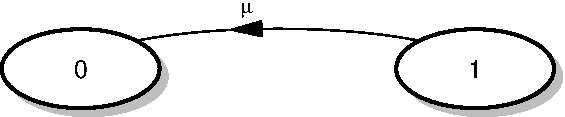
\includegraphics[width=0.95\linewidth]{04-CMTC_files/figure-latex/05-002-1} 

}

\caption{Diagrama de tasas para el tiempo de vida del Satélite}\label{fig:05-002}
\end{figure}

\begin{example}
\protect\hypertarget{exm:excmtc004}{}\label{exm:excmtc004}Continuando con el sistema del viajante descrito en el ejemplo \ref{exm:excmtc002} ya que conocemos las tasas medias y las probabilidades de salto podemos obtener la matriz \(R\) de forma inmediata:
\end{example}

\begin{Shaded}
\begin{Highlighting}[]
\NormalTok{estados }\OtherTok{\textless{}{-}} \FunctionTok{c}\NormalTok{(}\StringTok{"0"}\NormalTok{, }\StringTok{"1"}\NormalTok{, }\StringTok{"2"}\NormalTok{)}
\NormalTok{nestados }\OtherTok{\textless{}{-}} \FunctionTok{length}\NormalTok{(estados)}

\NormalTok{P }\OtherTok{\textless{}{-}} \FunctionTok{matrix}\NormalTok{(}\AttributeTok{nrow =}\NormalTok{ nestados, }\AttributeTok{ncol =}\NormalTok{ nestados, }
            \AttributeTok{data =} \FunctionTok{c}\NormalTok{(}\DecValTok{0}\NormalTok{, }\FloatTok{0.5}\NormalTok{, }\FloatTok{0.5}\NormalTok{, }\FloatTok{0.75}\NormalTok{, }\DecValTok{0}\NormalTok{, }\FloatTok{0.25}\NormalTok{, }\FloatTok{0.75}\NormalTok{, }\FloatTok{0.25}\NormalTok{, }\DecValTok{0}\NormalTok{), }
            \AttributeTok{byrow =} \DecValTok{3}\NormalTok{)}
\NormalTok{r }\OtherTok{\textless{}{-}} \FunctionTok{matrix}\NormalTok{(}\AttributeTok{nrow =}\NormalTok{ nestados, }\AttributeTok{ncol =}\NormalTok{ nestados, }
            \AttributeTok{data =} \FunctionTok{rep}\NormalTok{(}\FunctionTok{c}\NormalTok{(}\FloatTok{0.5}\NormalTok{, }\DecValTok{1}\NormalTok{, }\FloatTok{1.5}\NormalTok{),}\DecValTok{3}\NormalTok{))}

\NormalTok{R }\OtherTok{\textless{}{-}}\NormalTok{ P}\SpecialCharTok{*}\NormalTok{r}
\NormalTok{R}
\end{Highlighting}
\end{Shaded}

\begin{verbatim}
##       [,1]  [,2] [,3]
## [1,] 0.000 0.250 0.25
## [2,] 0.750 0.000 0.25
## [3,] 1.125 0.375 0.00
\end{verbatim}

de forma que el diagrama de tasas viene dado por (asignamos el valor de la ciudad a cada uno de los posibles estados del sistema)

\begin{figure}

{\centering 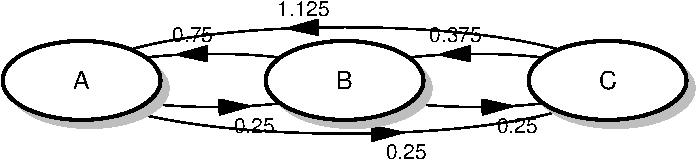
\includegraphics[width=0.95\linewidth]{04-CMTC_files/figure-latex/05-004-1} 

}

\caption{Diagrama de tasas para el proceso del vendedor}\label{fig:05-004}
\end{figure}

El diagrama representa el comportamiento de todo el proceso de viajes y estancias del vendedor.

\begin{example}
\protect\hypertarget{exm:excmtc005}{}\label{exm:excmtc005}\textbf{Sistema vida útil de una máquina}. Consideramos un sistema compuesto por una máquina que funciona durante un cantidad de tiempo que viene determianda por una variable aleatoria \(Exp(\mu)\) hasta que falla. Una vez se detecta la avería, la máquina se repara. El tiempo de reparación es una variable aleatoria \(Exp(\lambda)\) y es independiente del pasado. La máquina está como nueva después de la reparación. Sea \(X(t)\) el estado de la máquina en tiempo \(t\), de forma que toma el valor 1 si está en marcha y 0 si está parada (porque está siendo reparada).
\end{example}

En esta situación el tiempo de estancia en el estado 0 es el tiempo de reparación, de forma que \(r_0 = \lambda\), mientras que el tiempo en el estado 1 es el tiempo de funcionamiento con \(r_1 = \mu\). Además las probabiliddes de salto de interés son \(p_{01} = 1\) y \(p_{10} = 1\), dado que la máquina siempre es reparada y vuelve a funcionar, y porque sabemos que la máquina debe estropearse en algún momento.

El proceso definido de esta forma \(\{X_t; t \geq 0\}\) es una CMTC cuya matriz de tasas y matriz generadora del sistema vienen dadas por:

\[R = 
\begin{pmatrix}
0 & \lambda \\
\mu & 0
\end{pmatrix} \quad \text{ y } \quad Q = 
\begin{pmatrix}
-\lambda & \lambda \\
\mu & -\mu
\end{pmatrix}\]

El diagrama del sistema viene dado por:

\begin{figure}

{\centering 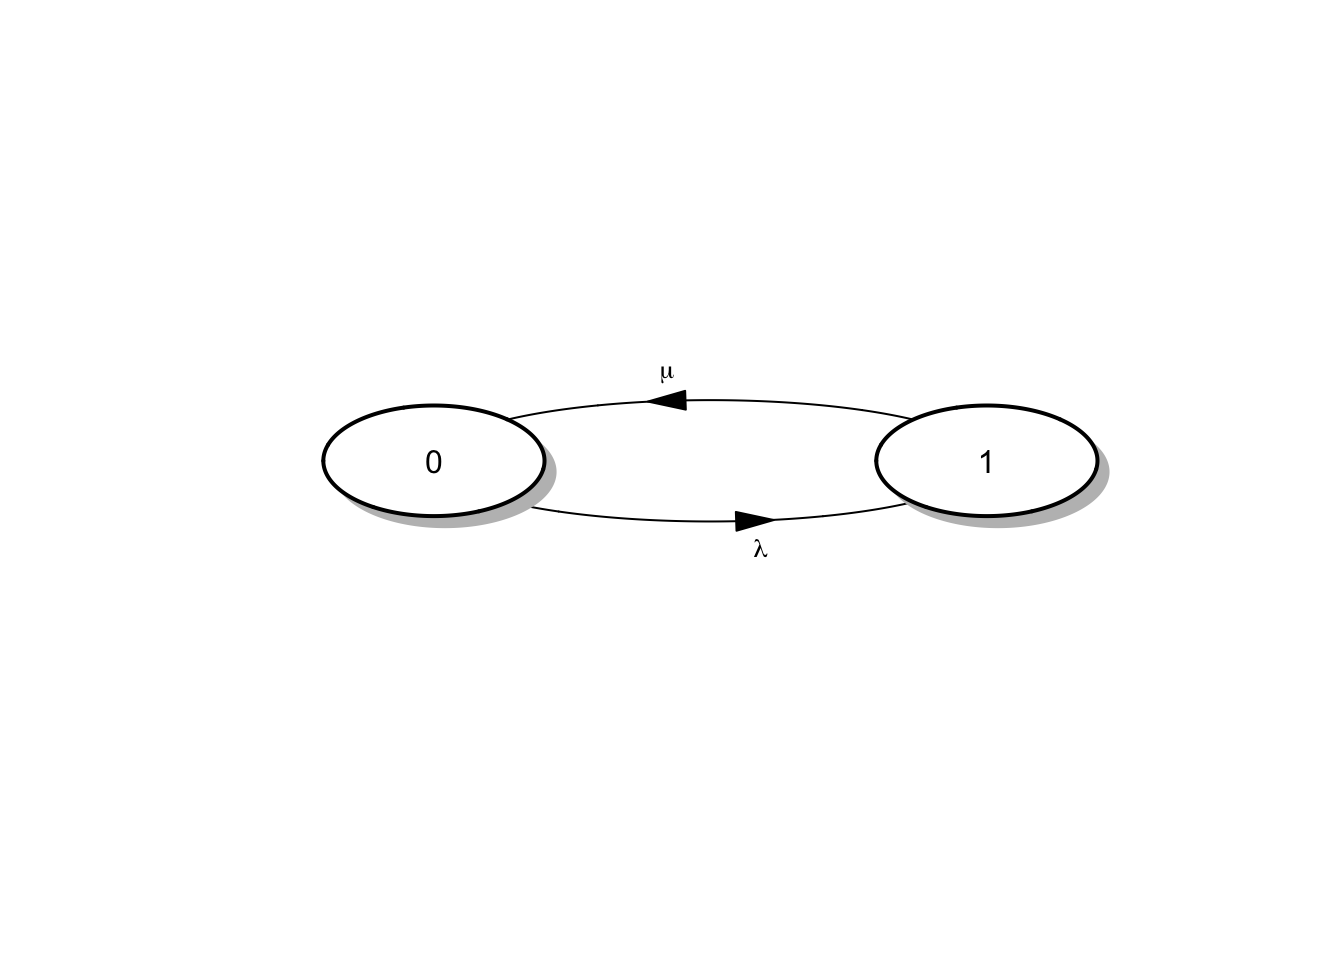
\includegraphics[width=0.95\linewidth]{04-CMTC_files/figure-latex/05-005-1} 

}

\caption{Diagrama de tasas para el sistema de una máquina}\label{fig:05-005}
\end{figure}

\hypertarget{CMTCC}{%
\section{Análisis preliminar del proceso}\label{CMTCC}}

Aunque más adelante estudiaremos los aspectos teóricos para el análisis completo de una CMTC, en este punto utilizamos la simulación del sistema para analizar su comportamiento. Nos centramos en las herramientas de simulación estudiadas hasta este punto para más adelante presentar con detalle la librería \texttt{simmer} que nos permite simular procesos y sistemas complejos.

Utilizamos los ejemplos \ref{exm:excmtc002} y \ref{exm:excmtc005} para mostrar cómo analizar un sistema, dado que el descrito en el ejemplo \ref{exm:excmtc001} se puede analizar sin más que describir la tasa del tiempo de vida del satélite.

\hypertarget{sistema-de-vida-uxfatil-de-una-muxe1quina}{%
\subsection{Sistema de vida útil de una máquina}\label{sistema-de-vida-uxfatil-de-una-muxe1quina}}

Comenzamos con el ejemplo \ref{exm:excmtc005}, para el que vamos a construir un algoritmo con el que simular el sistema hasta cierto instante de tiempo.

\begin{silverbox}
Algoritmo para el sistema de vida útil de una máquina:

\begin{enumerate}
\def\labelenumi{\arabic{enumi}.}
\tightlist
\item
  Fijar tasas de funcionamiento \(\mu\) y reparación \(\lambda\), así como el tiempo en que el sistema estará funcionando (\(tfin\)).
\item
  Fijar el tiempo de funcionamiento \(tfun = 0\), tiempo de reparación \(trep = 0\), y tiempo de funcionamiento del sistema \(tsis = tfun + trep\).
\item
  Fijar el número de vistas al estado de funcionamiento \(nfun = 0\) y al estado de reparación \(nrep =0\).
\end{enumerate}

Repetir los pasos siguientes hasta abandonar el sistema:

\begin{enumerate}
\def\labelenumi{\arabic{enumi}.}
\setcounter{enumi}{2}
\tightlist
\item
  Generar \(tfun \sim Exp(\mu)\) actualizando \(tsis\) y \(nfun\).
\item
  Si \(tsis > tfin\), abandonar el sistema.
\item
  Generar \(trep \sim Exp(\lambda)\) actualizando \(tsis\) y \(nrep\).
\item
  Si \(tsis > tfin\), abandonar el sistema.
\end{enumerate}

Los valores \(tfun\), \(trep\), así como las veces que se visitan los estados de funcionamiento y reparación nos permiten describir el funcionamiento del sistema para un tiempo prefijado.

\end{silverbox}

Para facilitar el análisis establecemos que todos los tiempos del sistema están en días y que deseamos estudiar el sistema durante un año. Creamos una función que nos permite modificar los valores de la tasa del tiempo de funcionamiento (recíproco de la media de tiempo en funcionamiento ), la tasa de reparación (recíproco de la media del tiempo de reparación) y el tiempo total de funcionamiento del sistema. Almacenamos los resultados de cada paso por el sistema para poder realizar los análisis correspondientes.

\begin{Shaded}
\begin{Highlighting}[]
\NormalTok{TSIM\_one\_machine }\OtherTok{\textless{}{-}} \ControlFlowTok{function}\NormalTok{(tasafun, tasarep, tfin)}
\NormalTok{\{}
  \CommentTok{\# Parámetros de la función}
  \CommentTok{\# =========================}
  \CommentTok{\# tasafun: tasa de funcionamiento}
  \CommentTok{\# tasarep: tasa de reparación}
  \CommentTok{\# tfin: tiempo de funcionamiento del sistema}
  
  \CommentTok{\# inicialización de parámetros del sistema }
\NormalTok{  tfun }\OtherTok{=}\NormalTok{ trep }\OtherTok{=}\NormalTok{ nfun }\OtherTok{=}\NormalTok{ nrep }\OtherTok{=}\NormalTok{ tsis }\OtherTok{=} \FunctionTok{vector}\NormalTok{()}
  \CommentTok{\# estado inicial del sistema}
\NormalTok{  i }\OtherTok{\textless{}{-}} \DecValTok{1}
\NormalTok{  tfun[i] }\OtherTok{=}\NormalTok{ trep [i] }\OtherTok{=}\NormalTok{ nfun[i] }\OtherTok{=}\NormalTok{ nrep[i] }\OtherTok{=} \DecValTok{0}
\NormalTok{  tsis[i] }\OtherTok{\textless{}{-}}\NormalTok{ tfun[i] }\SpecialCharTok{+}\NormalTok{ trep[i]}
  
  \CommentTok{\# Fijamos semilla}
  \FunctionTok{set.seed}\NormalTok{(}\DecValTok{123}\NormalTok{)}
  \CommentTok{\# Bucle de simulación}
  \ControlFlowTok{while}\NormalTok{(tsis[i] }\SpecialCharTok{\textless{}=}\NormalTok{ tfin)}
\NormalTok{  \{}
\NormalTok{    i}\OtherTok{\textless{}{-}}\NormalTok{ i }\SpecialCharTok{+} \DecValTok{1}
    \CommentTok{\# Máquina en funcionamiento}
\NormalTok{    nfun[i] }\OtherTok{=}\NormalTok{ nfun[i}\DecValTok{{-}1}\NormalTok{] }\SpecialCharTok{+} \DecValTok{1}
\NormalTok{    tfun[i] }\OtherTok{=} \FunctionTok{rexp}\NormalTok{(}\DecValTok{1}\NormalTok{, tasafun) }
\NormalTok{    tsis[i] }\OtherTok{=}\NormalTok{ tsis[i}\DecValTok{{-}1}\NormalTok{] }\SpecialCharTok{+}\NormalTok{ tfun[i]}
\NormalTok{    trep[i] }\OtherTok{=} \DecValTok{0} \CommentTok{\#Actualizamos estos dos parámetros ya que no hemos entrado en reparación}
\NormalTok{    nrep[i] }\OtherTok{=}\NormalTok{ nrep[i}\DecValTok{{-}1}\NormalTok{]}
    \ControlFlowTok{if}\NormalTok{(tsis[i] }\SpecialCharTok{\textgreater{}}\NormalTok{ tfin) \{}
      \CommentTok{\# adaptamos valores para quedarnos en los 365 días}
\NormalTok{      tfun[i] }\OtherTok{\textless{}{-}}\NormalTok{ tfin }\SpecialCharTok{{-}}\NormalTok{ tsis[i}\DecValTok{{-}1}\NormalTok{]}
\NormalTok{      tsis[i] }\OtherTok{\textless{}{-}}\NormalTok{ tsis[i}\DecValTok{{-}1}\NormalTok{] }\SpecialCharTok{+}\NormalTok{ tfun[i]}
      \ControlFlowTok{break}
\NormalTok{      \}}
    \CommentTok{\# Máquina en reparación}
\NormalTok{    nrep[i] }\OtherTok{=}\NormalTok{ nrep[i}\DecValTok{{-}1}\NormalTok{] }\SpecialCharTok{+} \DecValTok{1}
\NormalTok{    trep[i] }\OtherTok{=} \FunctionTok{rexp}\NormalTok{(}\DecValTok{1}\NormalTok{, tasarep)}
\NormalTok{    tsis[i] }\OtherTok{=}\NormalTok{ tsis[i] }\SpecialCharTok{+}\NormalTok{ trep[i]}
    \ControlFlowTok{if}\NormalTok{(tsis[i] }\SpecialCharTok{\textgreater{}}\NormalTok{ tfin) \{}
    \CommentTok{\# adaptamos valores para quedarnos en los 365 días}
\NormalTok{      trep[i] }\OtherTok{\textless{}{-}}\NormalTok{ tfin }\SpecialCharTok{{-}}\NormalTok{ tsis[i}\DecValTok{{-}1}\NormalTok{] }
\NormalTok{      tsis[i] }\OtherTok{=}\NormalTok{ tsis[i] }\SpecialCharTok{+}\NormalTok{ trep[i]}
      \ControlFlowTok{break}
\NormalTok{      \}}
\NormalTok{  \}}
\NormalTok{  res }\OtherTok{\textless{}{-}} \FunctionTok{tibble}\NormalTok{(tfun, nfun, trep, nrep, tsis)}
  \CommentTok{\# Devolvemos resultados del sistema quitando la fila de inicialización}
  \FunctionTok{return}\NormalTok{(res[}\SpecialCharTok{{-}}\DecValTok{1}\NormalTok{,])}
\NormalTok{\}}
\end{Highlighting}
\end{Shaded}

Supongamos que a través de los registros históricos de funcionamiento y reparación de la máquina se sabe que el tiempo medio de funcionamiento es de 60 días (\(\mu = 1/60\)) y el tiempo medio de reparación es de cuatro días (\(\lambda = 1/4\)). Además se está interesado en estudiar el funcionamiento del sistema para el próximo año (365 días). Queremos pues, estimar:

\begin{itemize}
\tightlist
\item
  Proporción del tiempo que la máquina está funcionando y en reparación.
\item
  Número de ocasiones en que la máquina debe ser reparada.
\item
  Si el beneficio neto es de 100 euros por cada día que la máquina está funcionando y una pérdida de 1500 euros por cada día que está en reparación ¿cuál es el beneficio esperado para el próximo año?
\end{itemize}

Obtenemos la simulación del sistema:

\begin{Shaded}
\begin{Highlighting}[]
\NormalTok{mu }\OtherTok{\textless{}{-}} \DecValTok{1}\SpecialCharTok{/}\DecValTok{60}
\NormalTok{lambda }\OtherTok{\textless{}{-}} \DecValTok{1}\SpecialCharTok{/}\DecValTok{4}
\NormalTok{simulacion }\OtherTok{\textless{}{-}} \FunctionTok{TSIM\_one\_machine}\NormalTok{(mu, lambda, }\DecValTok{365}\NormalTok{)}
\NormalTok{simulacion}
\end{Highlighting}
\end{Shaded}

\begin{verbatim}
## # A tibble: 6 x 5
##     tfun  nfun  trep  nrep  tsis
##    <dbl> <dbl> <dbl> <dbl> <dbl>
## 1  50.6      1 2.31      1  52.9
## 2  79.7      2 0.126     2 133. 
## 3   3.37     3 1.27      3 137. 
## 4  18.9      4 0.581     4 157. 
## 5 164.       5 0.117     5 321. 
## 6  44.5      6 0         5 365
\end{verbatim}

Podemos ver que el número de ciclos en que la máquina esta en fucionamiento es 6 mientras que el número de veces que ha necesitado reparación son 5.

Calculamos ahora los tiempos totales de funcionamiento y reparación:

\begin{Shaded}
\begin{Highlighting}[]
\NormalTok{tiempos }\OtherTok{\textless{}{-}} \FunctionTok{apply}\NormalTok{(simulacion[}\FunctionTok{c}\NormalTok{(}\DecValTok{1}\NormalTok{,}\DecValTok{3}\NormalTok{)], }\DecValTok{2}\NormalTok{, sum)}
\NormalTok{tiempos}
\end{Highlighting}
\end{Shaded}

\begin{verbatim}
##       tfun       trep 
## 360.603564   4.396436
\end{verbatim}

Por tanto, la proporción de tiempo que la máquina está en funcionamiento es 0.99, y el beneficio estimado para el próximo año viene dado por:

\begin{Shaded}
\begin{Highlighting}[]
\NormalTok{beneficio }\OtherTok{\textless{}{-}} \DecValTok{100} \SpecialCharTok{*}\NormalTok{ tiempos[}\StringTok{"tfun"}\NormalTok{] }\SpecialCharTok{{-}} \DecValTok{1500} \SpecialCharTok{*}\NormalTok{ tiempos[}\StringTok{"trep"}\NormalTok{]}
\NormalTok{beneficio}
\end{Highlighting}
\end{Shaded}

\begin{verbatim}
##    tfun 
## 29465.7
\end{verbatim}

\hypertarget{sistema-del-viajante}{%
\subsection{Sistema del viajante}\label{sistema-del-viajante}}

A continuación analizamos el sistema del viajante correspondiente al ejemplo \ref{exm:excmtc002}. En primer lugar establecemos el algoritmo de simulación del sistema. Para facilitar todas las posibilidades del algoritmo asumimos que el vendedor comienza el recorrido en la ciudad en la que reside.

\begin{silverbox}
Algoritmo para el análisis del sistema del viajante:

\begin{enumerate}
\def\labelenumi{\arabic{enumi}.}
\tightlist
\item
  Fijar tasas de permanencia en cada ciudad \(\mu_A\), \(\mu_B\), y \(\mu_C\), así como las probabilidades de salto dadas en la matriz \(P\), y una varibale que indica la ciudad en la que nos encontramos (\(ciudad\)).
\item
  Fijar el tiempo de funcionamiento del sistema \(tsis = 0\), tiempo de permanencia en cada ciudad \(tiempo = 0\), y el tiempo de estudio \(tfin\).
\item
  Generar \(tiempo \sim Exp(\mu_a)\) y actualizar \(tsis\), de forma que si \(tsis > tfin\) abandonamos el sistema.
\item
  Generamos un salto de la ciudad \(A\) de acuerdo a las probabilidades de \(P\) correspondientes a la ciudad \(A\).
\end{enumerate}

Repetir los pasos siguientes hasta que el tiempo en el sistema supere el tiempo fijado:

\begin{enumerate}
\def\labelenumi{\arabic{enumi}.}
\setcounter{enumi}{4}
\tightlist
\item
  Actualizamos \(ciudad\), generamos \(tiempo \sim Exp(\mu_{ciudad})\) y actualizamos \(tsis\), de forma que si \(tsis > tfin\) abandonamos el sistema.
\item
  Generamos un salto de la ciudad del paso anterior de acuerdo a las probabilidades de \(P\) correspondientes a dicha ciudad.
\end{enumerate}

Los valores \(tiempo\), y \(ciudad\) nos permiten describir el funcionamiento del sistema para un tiempo prefijado.

\end{silverbox}

A continuación construimos la función para simular el sistema hasta cierto instante de tiempo.

\begin{Shaded}
\begin{Highlighting}[]
\NormalTok{TSIM\_viajante }\OtherTok{\textless{}{-}} \ControlFlowTok{function}\NormalTok{(tasaA, tasaB, tasaC, tfin)}
\NormalTok{\{}
  \CommentTok{\# Parámetros de la función}
  \CommentTok{\# =========================}
  \CommentTok{\# tasaA: tasa de permanencia en A}
  \CommentTok{\# tasaB: tasa de permanencia en B}
  \CommentTok{\# tasaC: tasa de permanencia en C}
  \CommentTok{\# tfin: tiempo de funcionamiento del sistema}
  
  \CommentTok{\# inicialización de parámetros del sistema }
\NormalTok{  tiempo }\OtherTok{=}\NormalTok{ tsis }\OtherTok{=}\NormalTok{ ciudad }\OtherTok{=} \FunctionTok{vector}\NormalTok{()}
  \CommentTok{\# Probabilidades de salto. Fijamos la primera ya que la otra es complementaria}
\NormalTok{  pA }\OtherTok{\textless{}{-}} \FloatTok{0.5} \CommentTok{\# de A a B. De A a C es  1{-}pA}
\NormalTok{  pB }\OtherTok{\textless{}{-}} \FloatTok{0.75} \CommentTok{\# de B a A. De B a C es  1{-}pB}
\NormalTok{  pC }\OtherTok{\textless{}{-}} \FloatTok{0.75} \CommentTok{\# de C a A. De C a B es  1{-}pC}
  
  \CommentTok{\# estado inicial del sistema}
\NormalTok{  i }\OtherTok{\textless{}{-}} \DecValTok{1}
\NormalTok{  ciudad[i] }\OtherTok{\textless{}{-}} \StringTok{"A"}
  \CommentTok{\# Fijamos semilla}
  \FunctionTok{set.seed}\NormalTok{(}\DecValTok{123}\NormalTok{)}
  \CommentTok{\# Primer tiempo de estancia}
\NormalTok{  tiempo[i] }\OtherTok{=} \FunctionTok{rexp}\NormalTok{(}\DecValTok{1}\NormalTok{, tasaA)}
\NormalTok{  tsis[i] }\OtherTok{\textless{}{-}}\NormalTok{ tiempo[i]}
  \CommentTok{\# Saltamos de la ciudad A}
\NormalTok{  uniforme }\OtherTok{\textless{}{-}} \FunctionTok{runif}\NormalTok{(}\DecValTok{1}\NormalTok{)}
  \FunctionTok{ifelse}\NormalTok{(uniforme }\SpecialCharTok{\textless{}=}\NormalTok{ pA, ciudad[i}\SpecialCharTok{+}\DecValTok{1}\NormalTok{] }\OtherTok{\textless{}{-}} \StringTok{"B"}\NormalTok{, ciudad[i}\SpecialCharTok{+}\DecValTok{1}\NormalTok{] }\OtherTok{\textless{}{-}} \StringTok{"C"}\NormalTok{)}
      
  \CommentTok{\# Bucle de simulación}
  \ControlFlowTok{while}\NormalTok{(tsis[i] }\SpecialCharTok{\textless{}=}\NormalTok{ tfin)}
\NormalTok{  \{}
\NormalTok{    i}\OtherTok{\textless{}{-}}\NormalTok{ i }\SpecialCharTok{+} \DecValTok{1}
\NormalTok{    uniforme }\OtherTok{\textless{}{-}} \FunctionTok{runif}\NormalTok{(}\DecValTok{1}\NormalTok{)}
    \ControlFlowTok{if}\NormalTok{(ciudad[i] }\SpecialCharTok{==} \StringTok{"A"}\NormalTok{)}
\NormalTok{      \{}
        \CommentTok{\# Calculamos tiempo de permanencia}
\NormalTok{        tiempo[i] }\OtherTok{\textless{}{-}} \FunctionTok{rexp}\NormalTok{(}\DecValTok{1}\NormalTok{, tasaA)}
        \CommentTok{\# Actualizamos y valoramos si hemos alcanzado el tiempo límite}
\NormalTok{        tsis[i] }\OtherTok{=}\NormalTok{ tsis[i}\DecValTok{{-}1}\NormalTok{] }\SpecialCharTok{+}\NormalTok{ tiempo[i]}
        \ControlFlowTok{if}\NormalTok{(tsis[i] }\SpecialCharTok{\textgreater{}}\NormalTok{ tfin)\{}
\NormalTok{            tiempo[i] }\OtherTok{\textless{}{-}}\NormalTok{ tfin }\SpecialCharTok{{-}}\NormalTok{ tsis[i}\DecValTok{{-}1}\NormalTok{] }
\NormalTok{            tsis[i] }\OtherTok{=}\NormalTok{ tsis[i}\DecValTok{{-}1}\NormalTok{] }\SpecialCharTok{+}\NormalTok{ tiempo[i]}
            \ControlFlowTok{break}
\NormalTok{          \}}
        \CommentTok{\# Si no hemos alcanzado el límite realizamos un nuevo salto}
        \FunctionTok{ifelse}\NormalTok{(uniforme }\SpecialCharTok{\textless{}=}\NormalTok{ pA, ciudad[i}\SpecialCharTok{+}\DecValTok{1}\NormalTok{] }\OtherTok{\textless{}{-}} \StringTok{"B"}\NormalTok{, ciudad[i}\SpecialCharTok{+}\DecValTok{1}\NormalTok{] }\OtherTok{\textless{}{-}} \StringTok{"C"}\NormalTok{)}
\NormalTok{      \}}
    \ControlFlowTok{if}\NormalTok{(ciudad[i] }\SpecialCharTok{==} \StringTok{"B"}\NormalTok{)}
\NormalTok{      \{}
        \CommentTok{\# Calculamos tiempo de permanencia}
\NormalTok{        tiempo[i] }\OtherTok{\textless{}{-}} \FunctionTok{rexp}\NormalTok{(}\DecValTok{1}\NormalTok{, tasaB)}
        \CommentTok{\# Actualizamos y valoramos si hemos alcanzado el tiempo límite}
\NormalTok{        tsis[i] }\OtherTok{=}\NormalTok{ tsis[i}\DecValTok{{-}1}\NormalTok{] }\SpecialCharTok{+}\NormalTok{ tiempo[i]}
        \ControlFlowTok{if}\NormalTok{(tsis[i] }\SpecialCharTok{\textgreater{}}\NormalTok{ tfin)\{}
\NormalTok{            tiempo[i] }\OtherTok{\textless{}{-}}\NormalTok{ tfin }\SpecialCharTok{{-}}\NormalTok{ tsis[i}\DecValTok{{-}1}\NormalTok{] }
\NormalTok{            tsis[i] }\OtherTok{=}\NormalTok{ tsis[i}\DecValTok{{-}1}\NormalTok{] }\SpecialCharTok{+}\NormalTok{ tiempo[i]}
            \ControlFlowTok{break}
\NormalTok{          \}}
        \CommentTok{\# Si no hemos alcanzado el límite realizamos un nuevo salto}
        \FunctionTok{ifelse}\NormalTok{(uniforme }\SpecialCharTok{\textless{}=}\NormalTok{ pB, ciudad[i}\SpecialCharTok{+}\DecValTok{1}\NormalTok{] }\OtherTok{\textless{}{-}} \StringTok{"A"}\NormalTok{, ciudad[i}\SpecialCharTok{+}\DecValTok{1}\NormalTok{] }\OtherTok{\textless{}{-}} \StringTok{"C"}\NormalTok{)}
\NormalTok{      \}  }
    \ControlFlowTok{if}\NormalTok{(ciudad[i] }\SpecialCharTok{==} \StringTok{"C"}\NormalTok{)}
\NormalTok{      \{}
        \CommentTok{\# Calculamos tiempo de permanencia}
\NormalTok{        tiempo[i] }\OtherTok{\textless{}{-}} \FunctionTok{rexp}\NormalTok{(}\DecValTok{1}\NormalTok{, tasaC)}
        \CommentTok{\# Actualizamos y valoramos si hemos alcanzado el tiempo límite}
\NormalTok{        tsis[i] }\OtherTok{=}\NormalTok{ tsis[i}\DecValTok{{-}1}\NormalTok{] }\SpecialCharTok{+}\NormalTok{ tiempo[i]}
        \ControlFlowTok{if}\NormalTok{(tsis[i] }\SpecialCharTok{\textgreater{}}\NormalTok{ tfin)\{}
\NormalTok{            tiempo[i] }\OtherTok{\textless{}{-}}\NormalTok{ tfin }\SpecialCharTok{{-}}\NormalTok{ tsis[i}\DecValTok{{-}1}\NormalTok{] }
\NormalTok{            tsis[i] }\OtherTok{=}\NormalTok{ tsis[i}\DecValTok{{-}1}\NormalTok{] }\SpecialCharTok{+}\NormalTok{ tiempo[i]}
            \ControlFlowTok{break}
\NormalTok{          \}}
        \CommentTok{\# Si no hemos alcanzado el límite realizamos un nuevo salto}
        \FunctionTok{ifelse}\NormalTok{(uniforme }\SpecialCharTok{\textless{}=}\NormalTok{ pC, ciudad[i}\SpecialCharTok{+}\DecValTok{1}\NormalTok{] }\OtherTok{\textless{}{-}} \StringTok{"A"}\NormalTok{, ciudad[i}\SpecialCharTok{+}\DecValTok{1}\NormalTok{] }\OtherTok{\textless{}{-}} \StringTok{"C"}\NormalTok{)}
\NormalTok{      \}}
\NormalTok{  \}}
  \CommentTok{\# Devolvemos resultados del sistema }
\NormalTok{  ciudad }\OtherTok{\textless{}{-}} \FunctionTok{factor}\NormalTok{(ciudad)}
\NormalTok{  res }\OtherTok{\textless{}{-}} \FunctionTok{tibble}\NormalTok{(tiempo, ciudad, tsis)}
  \FunctionTok{return}\NormalTok{(res)}
\NormalTok{\}}
\end{Highlighting}
\end{Shaded}

Supongamos que estamos interesados en aproximar el comportamiento del vendedor durante el próximo año (52 semanas) para poder contestar a las preguntas siguientes:

\begin{itemize}
\tightlist
\item
  Proporción de tiempo que el vendedor pasa en cada ciudad.
\item
  Número de ocasiones en que visita cada ciudad.
\end{itemize}

Simulamos pues el sistema y contestamos a las preguntas planteadas:

\begin{Shaded}
\begin{Highlighting}[]
\NormalTok{tasaA }\OtherTok{\textless{}{-}} \DecValTok{1}\SpecialCharTok{/}\DecValTok{2}
\NormalTok{tasaB }\OtherTok{\textless{}{-}} \DecValTok{1}\SpecialCharTok{/}\DecValTok{1}
\NormalTok{tasaC }\OtherTok{\textless{}{-}} \DecValTok{2}\SpecialCharTok{/}\DecValTok{3}
\NormalTok{tfin }\OtherTok{\textless{}{-}} \DecValTok{52}
\NormalTok{simulacion }\OtherTok{\textless{}{-}} \FunctionTok{TSIM\_viajante}\NormalTok{(tasaA, tasaB, tasaC, tfin)  }
\CommentTok{\# Análsis del sistema}
\NormalTok{simulacion }\SpecialCharTok{\%\textgreater{}\%} 
  \FunctionTok{group\_by}\NormalTok{(ciudad) }\SpecialCharTok{\%\textgreater{}\%} 
  \FunctionTok{summarise}\NormalTok{(}\AttributeTok{visita =} \FunctionTok{n}\NormalTok{(), }\AttributeTok{estancia =} \FunctionTok{sum}\NormalTok{(tiempo)) }\SpecialCharTok{\%\textgreater{}\%}
  \FunctionTok{mutate}\NormalTok{(}\AttributeTok{proporcion =}\NormalTok{ estancia}\SpecialCharTok{/}\DecValTok{52}\NormalTok{)}
\end{Highlighting}
\end{Shaded}

\begin{verbatim}
## # A tibble: 3 x 4
##   ciudad visita estancia proporcion
##   <fct>   <int>    <dbl>      <dbl>
## 1 A          16     30.3      0.583
## 2 B           8     10.7      0.206
## 3 C          11     11.0      0.211
\end{verbatim}

\hypertarget{anuxe1lisis-con-simmer}{%
\subsection{Análisis con simmer}\label{anuxe1lisis-con-simmer}}

Si bien dedicamos en este curso un capítulo entero para contar el funcionamiento de la librería \texttt{simmer}, puesto que estos ejemplos son relativamente sencillos, podemos introducir sin demasiada complicación el algoritmo de simulación con \texttt{simmer}.

La libreria \texttt{simmer} permite simular de sistemas tanto continuos como discretos bajos dos premisas fundamentales:

\begin{itemize}
\tightlist
\item
  Proceso de llegadas (``arrivals'') al sistema.
\item
  Proceso de servicio (``server''): en el que a cada una de las llegadas se les asigna una serie de actividades a realizar (integradas en `trayectorias') y unos recursos o servidores que resuelven con ellas las actividades.
\end{itemize}

Para el sistema descrito en ejemplo \ref{exm:excmtc005} el proceso de llegadas viene identificado por las averías que se producen en determinados instantes de tiempo. El proceso de servicio se corresponde con las reparaciones de las máquinas, a las que se dedica cierto tiempo. En este caso el recurso es el reparador encargado de resolver la avería y poner en marcha la máquina de nuevo.

El primer paso del algoritmo de simulación es cargar las librerías y definir la semilla de simulación:

\begin{Shaded}
\begin{Highlighting}[]
\FunctionTok{library}\NormalTok{(simmer)}
\FunctionTok{library}\NormalTok{(simmer.plot)}
\FunctionTok{library}\NormalTok{(simmer.bricks)}
\FunctionTok{set.seed}\NormalTok{(}\DecValTok{1234}\NormalTok{)}
\end{Highlighting}
\end{Shaded}

Definimos ahora el entorno de simulación del sistema:

\begin{Shaded}
\begin{Highlighting}[]
\CommentTok{\# Tasas de permanencia del sistema}
\DocumentationTok{\#\#\#\#\#\#\#\#\#\#\#\#\#\#\#\#\#\#\#\#\#\#\#\#\#\#\#\#\#\#\#\#\#\#}
\NormalTok{lambda }\OtherTok{\textless{}{-}} \DecValTok{1}\SpecialCharTok{/}\DecValTok{4}  \CommentTok{\# tasa reparación}
\NormalTok{mu }\OtherTok{\textless{}{-}} \DecValTok{1}\SpecialCharTok{/}\DecValTok{60}     \CommentTok{\# tasa funcionamiento}

\CommentTok{\# Sistema}
\DocumentationTok{\#\#\#\#\#\#\#\#\#\#\#\#\#\#\#\#\#\#\#\#\#\#\#\#\#\#\#\#\#\#\#\#\#\#\#\#\#\#\#\#\#\#\#\#\#\#\#\#\#}
\NormalTok{sistema}\FloatTok{.1}\NormalTok{m }\OtherTok{\textless{}{-}} \ControlFlowTok{function}\NormalTok{(t, lambda, mu)}
\NormalTok{\{}
  \CommentTok{\# tarea dentro de sistema: reparación de las averías}
\NormalTok{  reparar }\OtherTok{\textless{}{-}} \FunctionTok{trajectory}\NormalTok{() }\SpecialCharTok{\%\textgreater{}\%}
    \CommentTok{\# la máquina estropeada se asigna a un reparador}
    \FunctionTok{seize}\NormalTok{(}\StringTok{"reparador"}\NormalTok{, }\AttributeTok{amount =} \DecValTok{1}\NormalTok{) }\SpecialCharTok{\%\textgreater{}\%}              
    \CommentTok{\# el tiempo de reparación es aleatorio}
    \FunctionTok{timeout}\NormalTok{(}\ControlFlowTok{function}\NormalTok{() }\FunctionTok{rexp}\NormalTok{(}\DecValTok{1}\NormalTok{, lambda)) }\SpecialCharTok{\%\textgreater{}\%}   
    \CommentTok{\# la máquina ya ha sido reparada}
    \FunctionTok{release}\NormalTok{(}\StringTok{"reparador"}\NormalTok{, }\AttributeTok{amount =} \DecValTok{1}\NormalTok{)               }

  \CommentTok{\# Configuración del sistema }
  \DocumentationTok{\#\#\#\#\#\#\#\#\#\#\#\#\#\#\#\#\#\#\#\#\#\#\#\#\#\#\#\#\#\#\#\#\#\#\#\#\#\#\#\#\#\#\#\#\#\#\#\#\#}
  \FunctionTok{simmer}\NormalTok{() }\SpecialCharTok{\%\textgreater{}\%}
    \CommentTok{\# Se definen los recursos: un único reparador y cola infinita}
    \FunctionTok{add\_resource}\NormalTok{(}\StringTok{"reparador"}\NormalTok{, }\AttributeTok{capacity =} \DecValTok{1}\NormalTok{) }\SpecialCharTok{\%\textgreater{}\%}           
    \CommentTok{\# Simulador de los tiempos entre averías, dirigidas a la trayectoria "reparar"}
    \FunctionTok{add\_generator}\NormalTok{(}\StringTok{"averia"}\NormalTok{, reparar, }\ControlFlowTok{function}\NormalTok{() }\FunctionTok{rexp}\NormalTok{(}\DecValTok{1}\NormalTok{, mu)) }\SpecialCharTok{\%\textgreater{}\%} 
    \CommentTok{\# Tiempo funcionamiento del sistema}
    \FunctionTok{run}\NormalTok{(}\AttributeTok{until =}\NormalTok{ t)     }
\NormalTok{\}}

\DocumentationTok{\#\#\# Simulación del sistema durante 365 días}
\NormalTok{operar }\OtherTok{\textless{}{-}} \FunctionTok{sistema.1m}\NormalTok{(}\DecValTok{365}\NormalTok{, }\DecValTok{1}\SpecialCharTok{/}\DecValTok{4}\NormalTok{, }\DecValTok{1}\SpecialCharTok{/}\DecValTok{60}\NormalTok{)}
\end{Highlighting}
\end{Shaded}

Analizamos ahora los resultados que proporciona el sistema simulado. Podemos acceder a las información de dos formas diferentes mediante las funciones \texttt{get\_mon\_arrivals()} para describir las llegadas (averías) y \texttt{get\_mon\_resources()} para describir la ocupación de los servidores recursos (técnicos reparadores).

\begin{Shaded}
\begin{Highlighting}[]
\NormalTok{reparacion }\OtherTok{=} \FunctionTok{get\_mon\_arrivals}\NormalTok{(operar)}
\NormalTok{reparacion}
\end{Highlighting}
\end{Shaded}

\begin{verbatim}
##      name start_time end_time activity_time finished replication
## 1 averia0   150.1055 150.1318    0.02632783     TRUE           1
## 2 averia1   164.9110 166.4598    1.54873033     TRUE           1
## 3 averia2   269.4758 272.7721    3.29632606     TRUE           1
## 4 averia3   274.8728 278.2250    3.35216128     TRUE           1
## 5 averia4   287.0299 294.5502    7.52030671     TRUE           1
## 6 averia5   332.6557 339.2903    6.63464954     TRUE           1
\end{verbatim}

El objeto resultante tiene las columnas siguientes:

\begin{itemize}
\tightlist
\item
  \texttt{name}: nombre de las llegadas (averías), numeradas correlativamente
\item
  \texttt{star\_time}: instante en el que llega al sistema (se produce la avería)
\item
  \texttt{end\_time}: instante en el que sale del sistema (se ha reparado)
\item
  \texttt{activity\_time}: tiempo dedicado a la tarea (tiempo de reparación)
\item
  \texttt{finished}: si la tarea ha finalizado dentro del periodo de tiempo de simulación establecido.
\item
  \texttt{replication}: número de replicas del sistema (1 porque sólo hemos lanzado una cadena).
\end{itemize}

\begin{Shaded}
\begin{Highlighting}[]
\NormalTok{recursos }\OtherTok{=} \FunctionTok{get\_mon\_resources}\NormalTok{(operar)}
\NormalTok{recursos}
\end{Highlighting}
\end{Shaded}

\begin{verbatim}
##     resource     time server queue capacity queue_size system limit replication
## 1  reparador 150.1055      1     0        1        Inf      1   Inf           1
## 2  reparador 150.1318      0     0        1        Inf      0   Inf           1
## 3  reparador 164.9110      1     0        1        Inf      1   Inf           1
## 4  reparador 166.4598      0     0        1        Inf      0   Inf           1
## 5  reparador 269.4758      1     0        1        Inf      1   Inf           1
## 6  reparador 272.7721      0     0        1        Inf      0   Inf           1
## 7  reparador 274.8728      1     0        1        Inf      1   Inf           1
## 8  reparador 278.2250      0     0        1        Inf      0   Inf           1
## 9  reparador 287.0299      1     0        1        Inf      1   Inf           1
## 10 reparador 294.5502      0     0        1        Inf      0   Inf           1
## 11 reparador 332.6557      1     0        1        Inf      1   Inf           1
## 12 reparador 339.2903      0     0        1        Inf      0   Inf           1
\end{verbatim}

Con la función \texttt{get\_mon\_resources()} tenemos una descripción continua de los recursos del proceso con las columnas:

\begin{itemize}
\tightlist
\item
  \texttt{resource}: recurso (numerado correlativamente si hubiera más de uno)
\item
  \texttt{time}: instante de tiempo en que se ha registrado alguna actividad (avería, reparación, puesta en marcha)
\item
  \texttt{server}: número de servidores (recursos) ocupados (como sólo hay un técnico, es igual a 1)
\item
  \texttt{queue}: llegadas en la cola (averías que están esperando ser reparadas porque el técnico está ocupado)
\item
  \texttt{capacity}: capacidad del sistema o número de reparadores en el sistema
\item
  \texttt{queue\_size}: tamaño de la cola de espera (averías en espera para ser reparadas)
\item
  \texttt{system}: llegadas en el sistema (número de averías en ese instante, en reparación o en cola)
\item
  \texttt{limit}: capacidad + tamaño de la cola
\item
  \texttt{replication}: número de replica del sistema (1 porque sólo se ha lanzado una cadena).
\end{itemize}

A partir de los resultados podemos responder a las mismas preguntas que ya planteamos antes:

\begin{itemize}
\tightlist
\item
  Proporción del tiempo que la máquina está funcionando y en reparación.
\item
  Número de ocasiones en que la máquina debe ser reparada.
\item
  Si el beneficio neto es de 100 euros por cada día que la máquina está funcionando y una pérdida de 1500 euros por cada día que está en reparación ¿cuál es el beneficio esperado para el próximo año?
\end{itemize}

Para responder al primer pregunta basta con sumar los tiempos de actividad y calcualr su proporción sobre los 365 días de simulación:

\begin{Shaded}
\begin{Highlighting}[]
\NormalTok{tiempo\_reparacion }\OtherTok{\textless{}{-}} \FunctionTok{sum}\NormalTok{(reparacion}\SpecialCharTok{$}\NormalTok{activity\_time)}
\NormalTok{propor }\OtherTok{\textless{}{-}} \FunctionTok{round}\NormalTok{(}\DecValTok{100}\SpecialCharTok{*}\NormalTok{(}\DecValTok{1}\SpecialCharTok{{-}}\NormalTok{(tiempo\_reparacion}\SpecialCharTok{/}\DecValTok{365}\NormalTok{)), }\DecValTok{2}\NormalTok{)}
\NormalTok{propor}
\end{Highlighting}
\end{Shaded}

\begin{verbatim}
## [1] 93.87
\end{verbatim}

La proporción de tiempo en que la máquina está funcionando es del 93.87\% y el tiempo que está en reparación es del 6.13\%.

El número de ocasiones en que la máquina está en reparación corresponde al número de veces que accedemos a la tarea de reparación, que en este caso es de 6.

Para calcular el beneficio obtenido a lo largo del año utilizamos el tiempo de reparación obtenido:

\begin{Shaded}
\begin{Highlighting}[]
\NormalTok{(}\DecValTok{365}\SpecialCharTok{{-}}\NormalTok{tiempo\_reparacion)}\SpecialCharTok{*}\DecValTok{100} \SpecialCharTok{{-}}\NormalTok{ tiempo\_reparacion}\SpecialCharTok{*}\DecValTok{1500}
\end{Highlighting}
\end{Shaded}

\begin{verbatim}
## [1] 694.3972
\end{verbatim}

Como se puede ver, los resultados no son muy similares a los obtenidos con el algoritmo que programamos nosotros. Para conseguir estimaciones estables deberíamos realizar diferentes replicaciones del sistema (lanzar varias cadenas) y promediar los beneficios obtenidos mediante un estimador Monte-Carlo. Podemos replicar fácilmente el sistema añadiendo dos líneas de código. Cada cadena replicada tendrá un distintivo diferente en el argumento `replicate' cuando monitorizamos los resultados.

\begin{Shaded}
\begin{Highlighting}[]
\CommentTok{\# lanzamos \textquotesingle{}nreplicas\textquotesingle{} de la cadena, que se almacenan en una lista}
\NormalTok{nreplicas }\OtherTok{\textless{}{-}} \DecValTok{500}
\NormalTok{envs }\OtherTok{\textless{}{-}} \FunctionTok{lapply}\NormalTok{(}\DecValTok{1}\SpecialCharTok{:}\NormalTok{nreplicas, }\ControlFlowTok{function}\NormalTok{(i)\{}
\NormalTok{  operar }\OtherTok{\textless{}{-}} \FunctionTok{sistema.1m}\NormalTok{(}\DecValTok{365}\NormalTok{, }\DecValTok{1}\SpecialCharTok{/}\DecValTok{4}\NormalTok{, }\DecValTok{1}\SpecialCharTok{/}\DecValTok{60}\NormalTok{)}
\NormalTok{\})}
\end{Highlighting}
\end{Shaded}

Ahora almacenamos todas las simulaciones a modo de matriz, en concreto `tibble', para poder realizar los cálculos oportunos agrupando por réplicas y con ellos poder calcular las estimaciones Monte-Carlo del tiempo total de reparación y del número de reparaciones.

\begin{Shaded}
\begin{Highlighting}[]
\CommentTok{\# guardamos todas las llegadas en formato \textquotesingle{}tibble\textquotesingle{}}
\NormalTok{simulaciones }\OtherTok{\textless{}{-}} \FunctionTok{as\_tibble}\NormalTok{(}\FunctionTok{get\_mon\_arrivals}\NormalTok{(envs))}

\CommentTok{\# agrupamos por \textquotesingle{}replication\textquotesingle{} para calcular los descriptivos de interés en cada réplica}
\NormalTok{salida }\OtherTok{\textless{}{-}}\NormalTok{ simulaciones }\SpecialCharTok{\%\textgreater{}\%} 
  \FunctionTok{group\_by}\NormalTok{(replication) }\SpecialCharTok{\%\textgreater{}\%} 
  \CommentTok{\# Calculamos los descriptivos por cada réplica}
  \FunctionTok{summarise}\NormalTok{(}\AttributeTok{nreparaciones =} \FunctionTok{n}\NormalTok{(), }
            \AttributeTok{tiempoparada =} \FunctionTok{sum}\NormalTok{(activity\_time)) }\SpecialCharTok{\%\textgreater{}\%} 
  \CommentTok{\# Calculamos las estimaciones Monte{-}Carlo con los descriptivos de las réplicas}
  \FunctionTok{summarise}\NormalTok{(}\AttributeTok{mmedia\_nrepara =} \FunctionTok{mean}\NormalTok{(nreparaciones),}
            \AttributeTok{min\_nrepara =} \FunctionTok{min}\NormalTok{(nreparaciones),}
            \AttributeTok{max\_nrepara =} \FunctionTok{max}\NormalTok{(nreparaciones),}
            \AttributeTok{media\_taveria =} \FunctionTok{mean}\NormalTok{(tiempoparada),}
            \AttributeTok{q25\_taveria =} \FunctionTok{quantile}\NormalTok{(tiempoparada, }\FloatTok{0.25}\NormalTok{),}
            \AttributeTok{q50\_taveria =} \FunctionTok{quantile}\NormalTok{(tiempoparada, }\FloatTok{0.50}\NormalTok{),}
            \AttributeTok{q75\_taveria =} \FunctionTok{quantile}\NormalTok{(tiempoparada, }\FloatTok{0.75}\NormalTok{),}
            \AttributeTok{sd\_taveria =} \FunctionTok{sd}\NormalTok{(tiempoparada) }
\NormalTok{            )}
\NormalTok{salida}
\end{Highlighting}
\end{Shaded}

\begin{verbatim}
## # A tibble: 1 x 8
##   mmedia_nrepara min_nrepara max_nrepara media_taveria q25_taveria q50_taveria q75_taveria
##            <dbl>       <int>       <int>         <dbl>       <dbl>       <dbl>       <dbl>
## 1           6.12           1          15          23.8        13.4        21.3        31.9
## # ... with 1 more variable: sd_taveria <dbl>
\end{verbatim}

En `mmedia\_nrepara' tenemos la estimación del número de reparaciones en un año, en `min\_nrepara' y `max\_nrepara' el mínimo y el máximo respectivamente; en `media\_taveria' tenemos una estimación del tiempo medio acumulado en reparaciones en un año, con sus cuartiles (q25, q50 y q75) y desviación típica (sd).

Así podemos calcular los beneficios esperados en función del número de días que la máquina funciona y los que está estropeada:

\begin{Shaded}
\begin{Highlighting}[]
\CommentTok{\# número de días en funcionamiento vs número de días en reparación}
\NormalTok{(}\DecValTok{365}\SpecialCharTok{{-}}\NormalTok{salida}\SpecialCharTok{$}\NormalTok{media\_taveria)}\SpecialCharTok{*}\DecValTok{100} \SpecialCharTok{{-}}\NormalTok{ salida}\SpecialCharTok{$}\NormalTok{media\_taveria}\SpecialCharTok{*}\DecValTok{1500}
\end{Highlighting}
\end{Shaded}

\begin{verbatim}
## [1] -1561.395
\end{verbatim}

Podemos considerar también otros dos escenarios posibles: uno pesimista, con un mayor tiempo acumulado de reparación (cuantil 75), y uno optimisma, con un menor tiempo (con el cuantil 25), y calcular con ellos los beneficios:

\begin{Shaded}
\begin{Highlighting}[]
\NormalTok{(}\DecValTok{365}\SpecialCharTok{{-}}\NormalTok{salida}\SpecialCharTok{$}\NormalTok{q75\_taveria)}\SpecialCharTok{*}\DecValTok{100} \SpecialCharTok{{-}}\NormalTok{ salida}\SpecialCharTok{$}\NormalTok{q75\_taveria}\SpecialCharTok{*}\DecValTok{1500}
\end{Highlighting}
\end{Shaded}

\begin{verbatim}
##       75% 
## -14480.82
\end{verbatim}

\begin{Shaded}
\begin{Highlighting}[]
\NormalTok{(}\DecValTok{365}\SpecialCharTok{{-}}\NormalTok{salida}\SpecialCharTok{$}\NormalTok{q25\_taveria)}\SpecialCharTok{*}\DecValTok{100} \SpecialCharTok{{-}}\NormalTok{ salida}\SpecialCharTok{$}\NormalTok{q25\_taveria}\SpecialCharTok{*}\DecValTok{1500}
\end{Highlighting}
\end{Shaded}

\begin{verbatim}
##      25% 
## 15047.35
\end{verbatim}

¿Qué conclusiones podemos extraer de este análisis?

Para finalizar este apartado presentamos un nuevo ejemplo donde el espacio de estados está compuesto por una pareja de valores y no por un único valor como en los ejemplos que hemos presentado hasta ahora.

\hypertarget{mantenimiento-de-aronaves}{%
\subsection{Mantenimiento de aronaves}\label{mantenimiento-de-aronaves}}

Una empresa de mantenimiento de aeronaves está interesada en el proceso de avería-reparación de cierto tipo de aviones. El tipo de avión de interés es un avión comercial a reacción con cuatro motores, dos en cada ala. Cuando un motor se enciende, el tiempo que se puede mantener en funcionamiento hasta que falla es una variable aleatoria exponencial con parámetro \(\lambda\). Si el fallo se produce en vuelo, no puede haber reparación, pero el avión necesita al menos un motor en cada ala para funcionar correctamente y poder volar con seguridad. En concreto, la empresa está interesada en poder predecir la probabilidad de un vuelo sin problemas.

Si denotamos por \(X_L(t)\) y \(X_R(t)\) el número de motores funcionando en el instante \(t\) en el ala izquierda y el ala derecha respectivamente, podemos considerar el estado del sistema en el instante \(t\) como \(X(t) = (X_L(t), X_R(t))\). Si asumimos que los fallos en los motores son independientes entre sí, podemos ver que el proceo \(\{X(t), t \geq 0\}\) es una CMTC con espacio de estados:

\[S = \{ (0, 0), (0, 1), (0, 2), (1, 0), (1, 1), (1, 2), (2, 0), (2, 1), (2,2) \}\]

En esta situación, el avión sigue funcionando en el subconjunto de estados \(S = \{ (1, 1), (1, 2), (2, 1), (2,2) \}\).

Vamos a asumir (aunque no es real) que el sistema sigue funcionando, incluso cuando hay posibilidad de un accidente, hasta que llegamos al estado \((0, 0)\). Dado que no hay reparación posible, la matriz de tasas entre estados del sistema viene dada por

\[R = 
\begin{pmatrix}
0 & 0 & 0 & 0 & 0 & 0 & 0 & 0 & 0 \\
\lambda & 0 & 0 & 0 & 0 & 0 & 0 & 0 & 0 \\
0 & 2\lambda & 0 & 0 & 0 & 0 & 0 & 0 & 0 \\
\lambda & 0 & 0 & 0 & 0 & 0 & 0 & 0 & 0 \\
0 & \lambda & 0 & \lambda & 0 & 0 & 0 & 0 & 0 \\
0 & 0 & \lambda & 0 & 2\lambda & 0 & 0 & 0 & 0 \\
0 & 0 & 0 & 2\lambda & 0 & 0 & 0 & 0 & 0 \\
0 & 0 & 0 & 0 & 2\lambda & 0 & 0 & 0 & 0 \\
0 & 0 & 0 & 0 & 0 & 2\lambda & 0 & 2\lambda & 0
\end{pmatrix} \]

y el diagrama que representa el sistema resulta:

\begin{figure}

{\centering 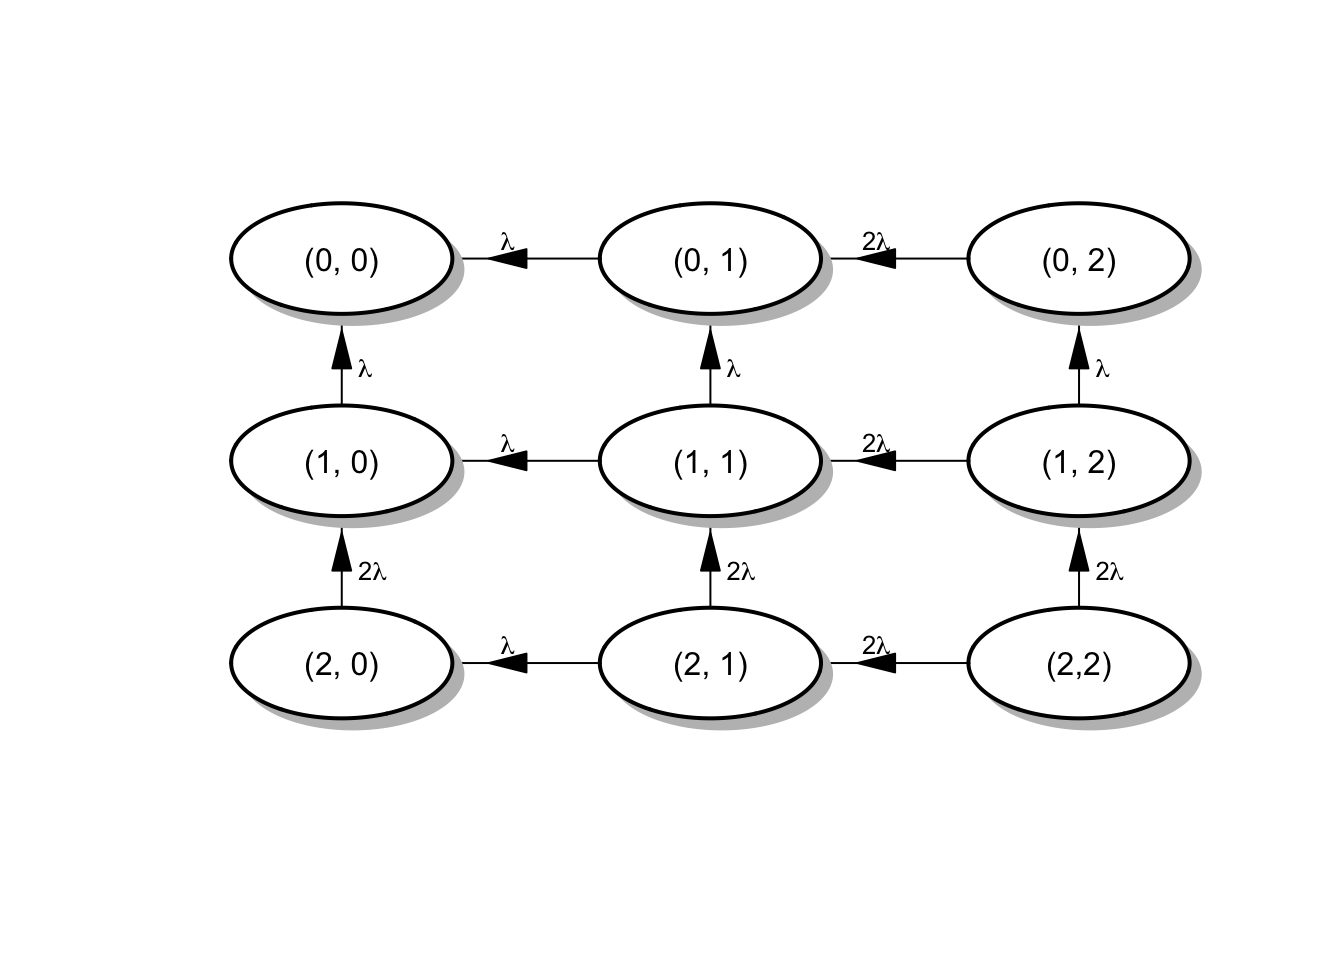
\includegraphics[width=0.95\linewidth]{04-CMTC_files/figure-latex/05-022-1} 

}

\caption{Diagrama de tasas para el sistema motores de aviones}\label{fig:05-022}
\end{figure}

Para facilitar el algoritmo de simulación en esta situación, vamos a asignar un código a cada uno de los posibles estados del sistema:

\[S = \{ 1 = (0, 0), 2 = (0, 1), 3 = (0, 2), 4 = (1, 0), 5 = (1, 1), 6 = (1, 2), 7 = (2, 0), 8 = (2, 1), 9 = (2,2) \}\]

y asumimos que la media del tiempo hasta que un motor falla cuando está encendido es de 20 horas, es decir, \(\lambda = 1/20\). A continuación hemos construido una función para simular el sistema descrito:

\begin{Shaded}
\begin{Highlighting}[]
\NormalTok{TSIM\_aviones }\OtherTok{\textless{}{-}} \ControlFlowTok{function}\NormalTok{(tasa)}
\NormalTok{\{}
  \CommentTok{\# Parámetros de la función}
  \CommentTok{\# =========================}
  \CommentTok{\# tasa: tasa de fallo de un motor}
  
  \CommentTok{\# Valores fijos del sistema}
  \CommentTok{\# codigos de motores funcionando obviando el estado inicial}
\NormalTok{  codigo }\OtherTok{\textless{}{-}} \DecValTok{1}\SpecialCharTok{:}\DecValTok{8}
  \CommentTok{\# motores con fallo de acuerdo al código}
\NormalTok{  motoresOFF }\OtherTok{\textless{}{-}} \FunctionTok{c}\NormalTok{(}\DecValTok{4}\NormalTok{, }\DecValTok{3}\NormalTok{, }\DecValTok{2}\NormalTok{, }\DecValTok{3}\NormalTok{, }\DecValTok{2}\NormalTok{, }\DecValTok{1}\NormalTok{, }\DecValTok{2}\NormalTok{, }\DecValTok{1}\NormalTok{)}
  
  \CommentTok{\# inicialización de parámetros del sistema }
\NormalTok{  tiempo }\OtherTok{=}\NormalTok{  estado }\OtherTok{=}\NormalTok{ fallos }\OtherTok{=} \FunctionTok{vector}\NormalTok{()}
\NormalTok{  i}\OtherTok{\textless{}{-}}\DecValTok{1}
  \CommentTok{\# Primer fallo}
  \CommentTok{\# Posibles estados de salto}
\NormalTok{  saltos }\OtherTok{=} \FunctionTok{c}\NormalTok{(codigo[}\DecValTok{6}\NormalTok{], codigo[}\DecValTok{8}\NormalTok{])}
  \CommentTok{\# tiempos asociados a cada fallo}
\NormalTok{  simula }\OtherTok{=} \FunctionTok{rexp}\NormalTok{(}\DecValTok{2}\NormalTok{, }\DecValTok{2}\SpecialCharTok{*}\NormalTok{tasa)}
  \CommentTok{\# Seleccionamos el salto}
\NormalTok{  posicion }\OtherTok{=} \FunctionTok{which.min}\NormalTok{(simula)}
  \ControlFlowTok{if}\NormalTok{(posicion }\SpecialCharTok{==} \DecValTok{1}\NormalTok{)}
\NormalTok{  \{}
\NormalTok{    estado[i] }\OtherTok{\textless{}{-}}\NormalTok{ saltos[posicion]}
\NormalTok{    tiempo[i] }\OtherTok{\textless{}{-}}\NormalTok{ simula[posicion] }
\NormalTok{    fallos[i] }\OtherTok{\textless{}{-}}\NormalTok{ motoresOFF[saltos[posicion]]}
    \CommentTok{\# nuevo salto}
\NormalTok{    i }\OtherTok{\textless{}{-}}\NormalTok{ i }\SpecialCharTok{+} \DecValTok{1}
\NormalTok{    saltos }\OtherTok{=} \FunctionTok{c}\NormalTok{(codigo[}\DecValTok{3}\NormalTok{], codigo[}\DecValTok{5}\NormalTok{])}
\NormalTok{    simula }\OtherTok{=} \FunctionTok{c}\NormalTok{(}\FunctionTok{rexp}\NormalTok{(}\DecValTok{1}\NormalTok{, tasa), }\FunctionTok{rexp}\NormalTok{(}\DecValTok{1}\NormalTok{, }\DecValTok{2}\SpecialCharTok{*}\NormalTok{tasa))}
\NormalTok{    posicion }\OtherTok{=} \FunctionTok{which.min}\NormalTok{(simula)}
    \ControlFlowTok{if}\NormalTok{(posicion }\SpecialCharTok{==} \DecValTok{1}\NormalTok{)}
\NormalTok{    \{}
\NormalTok{      estado[i] }\OtherTok{\textless{}{-}}\NormalTok{ saltos[posicion]}
\NormalTok{      tiempo[i] }\OtherTok{\textless{}{-}}\NormalTok{ simula[posicion] }
\NormalTok{      fallos[i] }\OtherTok{\textless{}{-}}\NormalTok{ motoresOFF[saltos[posicion]]}
      \CommentTok{\# dos últimos saltos}
\NormalTok{      estado[i}\SpecialCharTok{+}\DecValTok{1}\NormalTok{] }\OtherTok{\textless{}{-}} \DecValTok{2}\NormalTok{; estado[i}\SpecialCharTok{+}\DecValTok{2}\NormalTok{] }\OtherTok{\textless{}{-}} \DecValTok{1}
\NormalTok{      tiempo[i}\SpecialCharTok{+}\DecValTok{1}\NormalTok{] }\OtherTok{\textless{}{-}} \FunctionTok{rexp}\NormalTok{(}\DecValTok{1}\NormalTok{, }\DecValTok{2}\SpecialCharTok{*}\NormalTok{tasa); tiempo[i}\SpecialCharTok{+}\DecValTok{2}\NormalTok{] }\OtherTok{\textless{}{-}} \FunctionTok{rexp}\NormalTok{(}\DecValTok{1}\NormalTok{, tasa)}
\NormalTok{      fallos[i}\SpecialCharTok{+}\DecValTok{1}\NormalTok{] }\OtherTok{\textless{}{-}}\NormalTok{ motoresOFF[estado[i}\SpecialCharTok{+}\DecValTok{1}\NormalTok{]]; fallos[i}\SpecialCharTok{+}\DecValTok{2}\NormalTok{] }\OtherTok{\textless{}{-}}\NormalTok{ motoresOFF[estado[i}\SpecialCharTok{+}\DecValTok{2}\NormalTok{]]}
\NormalTok{    \}}
    \ControlFlowTok{else}
\NormalTok{    \{}
\NormalTok{      estado[i] }\OtherTok{\textless{}{-}}\NormalTok{ saltos[posicion]}
\NormalTok{      tiempo[i] }\OtherTok{\textless{}{-}}\NormalTok{ simula[posicion] }
\NormalTok{      fallos[i] }\OtherTok{\textless{}{-}}\NormalTok{ motoresOFF[saltos[posicion]]  }
      \CommentTok{\# dos últimos saltos}
\NormalTok{      estado[i}\SpecialCharTok{+}\DecValTok{1}\NormalTok{] }\OtherTok{\textless{}{-}} \DecValTok{2}\NormalTok{; estado[i}\SpecialCharTok{+}\DecValTok{2}\NormalTok{] }\OtherTok{\textless{}{-}} \DecValTok{1}
\NormalTok{      tiempo[i}\SpecialCharTok{+}\DecValTok{1}\NormalTok{] }\OtherTok{\textless{}{-}} \FunctionTok{rexp}\NormalTok{(}\DecValTok{1}\NormalTok{, tasa); tiempo[i}\SpecialCharTok{+}\DecValTok{2}\NormalTok{] }\OtherTok{\textless{}{-}} \FunctionTok{rexp}\NormalTok{(}\DecValTok{1}\NormalTok{, tasa)}
\NormalTok{      fallos[i}\SpecialCharTok{+}\DecValTok{1}\NormalTok{] }\OtherTok{\textless{}{-}}\NormalTok{ motoresOFF[estado[i}\SpecialCharTok{+}\DecValTok{1}\NormalTok{]]; fallos[i}\SpecialCharTok{+}\DecValTok{2}\NormalTok{] }\OtherTok{\textless{}{-}}\NormalTok{ motoresOFF[estado[i}\SpecialCharTok{+}\DecValTok{2}\NormalTok{]]}
\NormalTok{    \}}
\NormalTok{  \}}
  \ControlFlowTok{else}
\NormalTok{  \{}
\NormalTok{    estado[i] }\OtherTok{\textless{}{-}}\NormalTok{ saltos[posicion]}
\NormalTok{    tiempo[i] }\OtherTok{\textless{}{-}}\NormalTok{ simula[posicion] }
\NormalTok{    fallos[i] }\OtherTok{\textless{}{-}}\NormalTok{ motoresOFF[saltos[posicion]]}
    \CommentTok{\# nuevo salto}
\NormalTok{    i }\OtherTok{\textless{}{-}}\NormalTok{ i }\SpecialCharTok{+} \DecValTok{1}
\NormalTok{    saltos }\OtherTok{=} \FunctionTok{c}\NormalTok{(codigo[}\DecValTok{7}\NormalTok{], codigo[}\DecValTok{5}\NormalTok{])}
\NormalTok{    simula }\OtherTok{=} \FunctionTok{c}\NormalTok{(}\FunctionTok{rexp}\NormalTok{(}\DecValTok{1}\NormalTok{, tasa), }\FunctionTok{rexp}\NormalTok{(}\DecValTok{1}\NormalTok{, }\DecValTok{2}\SpecialCharTok{*}\NormalTok{tasa))}
\NormalTok{    posicion }\OtherTok{=} \FunctionTok{which.min}\NormalTok{(simula)}
    \ControlFlowTok{if}\NormalTok{(posicion }\SpecialCharTok{==} \DecValTok{1}\NormalTok{)}
\NormalTok{    \{}
\NormalTok{      estado[i] }\OtherTok{\textless{}{-}}\NormalTok{ saltos[posicion]}
\NormalTok{      tiempo[i] }\OtherTok{\textless{}{-}}\NormalTok{ simula[posicion] }
\NormalTok{      fallos[i] }\OtherTok{\textless{}{-}}\NormalTok{ motoresOFF[saltos[posicion]]}
      \CommentTok{\# dos últimos saltos}
\NormalTok{      estado[i}\SpecialCharTok{+}\DecValTok{1}\NormalTok{] }\OtherTok{\textless{}{-}} \DecValTok{2}\NormalTok{; estado[i}\SpecialCharTok{+}\DecValTok{2}\NormalTok{] }\OtherTok{\textless{}{-}} \DecValTok{1}
\NormalTok{      tiempo[i}\SpecialCharTok{+}\DecValTok{1}\NormalTok{] }\OtherTok{\textless{}{-}} \FunctionTok{rexp}\NormalTok{(}\DecValTok{1}\NormalTok{, }\DecValTok{2}\SpecialCharTok{*}\NormalTok{tasa); tiempo[i}\SpecialCharTok{+}\DecValTok{2}\NormalTok{] }\OtherTok{\textless{}{-}} \FunctionTok{rexp}\NormalTok{(}\DecValTok{1}\NormalTok{, tasa)}
\NormalTok{      fallos[i}\SpecialCharTok{+}\DecValTok{1}\NormalTok{] }\OtherTok{\textless{}{-}}\NormalTok{ motoresOFF[estado[i}\SpecialCharTok{+}\DecValTok{1}\NormalTok{]]; fallos[i}\SpecialCharTok{+}\DecValTok{2}\NormalTok{] }\OtherTok{\textless{}{-}}\NormalTok{ motoresOFF[estado[i}\SpecialCharTok{+}\DecValTok{2}\NormalTok{]]}
\NormalTok{    \}}
    \ControlFlowTok{else}
\NormalTok{    \{}
\NormalTok{      estado[i] }\OtherTok{\textless{}{-}}\NormalTok{ saltos[posicion]}
\NormalTok{      tiempo[i] }\OtherTok{\textless{}{-}}\NormalTok{ simula[posicion] }
\NormalTok{      fallos[i] }\OtherTok{\textless{}{-}}\NormalTok{ motoresOFF[saltos[posicion]]  }
      \CommentTok{\# dos últimos saltos}
\NormalTok{      estado[i}\SpecialCharTok{+}\DecValTok{1}\NormalTok{] }\OtherTok{\textless{}{-}} \DecValTok{2}\NormalTok{; estado[i}\SpecialCharTok{+}\DecValTok{2}\NormalTok{] }\OtherTok{\textless{}{-}} \DecValTok{1}
\NormalTok{      tiempo[i}\SpecialCharTok{+}\DecValTok{1}\NormalTok{] }\OtherTok{\textless{}{-}} \FunctionTok{rexp}\NormalTok{(}\DecValTok{1}\NormalTok{, tasa); tiempo[i}\SpecialCharTok{+}\DecValTok{2}\NormalTok{] }\OtherTok{\textless{}{-}} \FunctionTok{rexp}\NormalTok{(}\DecValTok{1}\NormalTok{, tasa)}
\NormalTok{      fallos[i}\SpecialCharTok{+}\DecValTok{1}\NormalTok{] }\OtherTok{\textless{}{-}}\NormalTok{ motoresOFF[estado[i}\SpecialCharTok{+}\DecValTok{1}\NormalTok{]]; fallos[i}\SpecialCharTok{+}\DecValTok{2}\NormalTok{] }\OtherTok{\textless{}{-}}\NormalTok{ motoresOFF[estado[i}\SpecialCharTok{+}\DecValTok{2}\NormalTok{]]}
\NormalTok{    \}    }
\NormalTok{  \}}

  \CommentTok{\# Devolvemos resultados del sistema }
\NormalTok{  res }\OtherTok{\textless{}{-}} \FunctionTok{tibble}\NormalTok{(estado, tiempo, fallos)}
  \FunctionTok{return}\NormalTok{(res)}
\NormalTok{\}}
\end{Highlighting}
\end{Shaded}

Veamos una simulación del sistema:

\begin{Shaded}
\begin{Highlighting}[]
\FunctionTok{set.seed}\NormalTok{(}\DecValTok{12}\NormalTok{)}
\NormalTok{tasa }\OtherTok{\textless{}{-}} \DecValTok{1}\SpecialCharTok{/}\DecValTok{20}
\NormalTok{sistema }\OtherTok{\textless{}{-}} \FunctionTok{TSIM\_aviones}\NormalTok{(tasa)}
\NormalTok{sistema}
\end{Highlighting}
\end{Shaded}

\begin{verbatim}
## # A tibble: 4 x 3
##   estado tiempo fallos
##    <dbl>  <dbl>  <dbl>
## 1      8   6.36      1
## 2      7   2.35      2
## 3      2  18.2       3
## 4      1   5.67      4
\end{verbatim}

El resultado obtenido es el estado en cada paso del algoritmo hasta llegar a la parada total, los tiempos para alcanzar cada estado, y el número de motores con fallo.

Podemos operar los tiempos para saber cuándo tendremos más de dos motores con fallo (últimas dos filas de la simulación).

Si el vuelo que acabamos de empezar es de \(x\) horas ¿cómo podemos estimar la probabilidad de no poder terminar el vuelo de forma segura? Para responder esta pregunta podremos calcular la proporción de tiempo que corresponde con un fallo leve (1 o 2 motores con fallo) con respecto a las \(x\) horas de duración del vuelo.

Calculamos a continuación el tiempo de fallo del sistema y evaluamos la probabilidad para diferentes tiempos de duración de vuelo.

\begin{Shaded}
\begin{Highlighting}[]
\CommentTok{\# Tiempo de fallo}
\NormalTok{Tfallo }\OtherTok{\textless{}{-}} \FunctionTok{round}\NormalTok{(}\FunctionTok{sum}\NormalTok{(sistema}\SpecialCharTok{$}\NormalTok{tiempo[sistema}\SpecialCharTok{$}\NormalTok{fallos }\SpecialCharTok{\textless{}=} \DecValTok{2}\NormalTok{]), }\DecValTok{2}\NormalTok{)}
\CommentTok{\# Duración del vuelo}
\NormalTok{td }\OtherTok{\textless{}{-}} \FunctionTok{seq}\NormalTok{(}\FloatTok{0.1}\NormalTok{, }\DecValTok{12}\NormalTok{, }\AttributeTok{by =} \FloatTok{0.1}\NormalTok{)}
\NormalTok{prob }\OtherTok{\textless{}{-}} \FunctionTok{vector}\NormalTok{()}
\CommentTok{\# Probabilidad viaje seguro}
\ControlFlowTok{for}\NormalTok{(i }\ControlFlowTok{in} \DecValTok{1}\SpecialCharTok{:}\FunctionTok{length}\NormalTok{(td))}
\NormalTok{\{}
\NormalTok{  prob[i] }\OtherTok{\textless{}{-}} \FunctionTok{ifelse}\NormalTok{(Tfallo }\SpecialCharTok{\textgreater{}=}\NormalTok{ td[i], }\DecValTok{1}\NormalTok{, }\FunctionTok{round}\NormalTok{(Tfallo}\SpecialCharTok{/}\NormalTok{td[i], }\DecValTok{3}\NormalTok{))}
\NormalTok{\}}
\CommentTok{\# Obtenemos el valor mínimo de tiempo para asegurar un viaje seguro}
\NormalTok{limite }\OtherTok{\textless{}{-}} \FunctionTok{min}\NormalTok{(td[}\FunctionTok{which}\NormalTok{(prob }\SpecialCharTok{!=} \DecValTok{1}\NormalTok{)])}
\NormalTok{limite}
\end{Highlighting}
\end{Shaded}

\begin{verbatim}
## [1] 8.8
\end{verbatim}

Cualquier viaje inferior a 8.8 horas será un viaje seguro, mientras que si el tiempo es superior, la probabilidad de no tener un viaje seguro aumenta.

Para estudiar la estabilidad de dichas probabilidades realizamos 1000 simulaciones del sistema y estimamos las probabilidades mediante estimadores Monte-Carlo de los tiempos de fallo.

\begin{Shaded}
\begin{Highlighting}[]
\NormalTok{nsim }\OtherTok{\textless{}{-}} \DecValTok{1000}
\NormalTok{Tfallo }\OtherTok{\textless{}{-}} \FunctionTok{vector}\NormalTok{()}
\CommentTok{\# Repetición del sistema y calculo de tiempo }
\ControlFlowTok{for}\NormalTok{(i }\ControlFlowTok{in} \DecValTok{1}\SpecialCharTok{:}\NormalTok{nsim)}
\NormalTok{\{}
\NormalTok{  sistema }\OtherTok{\textless{}{-}} \FunctionTok{TSIM\_aviones}\NormalTok{(tasa)}
\NormalTok{  Tfallo[i] }\OtherTok{\textless{}{-}} \FunctionTok{round}\NormalTok{(}\FunctionTok{sum}\NormalTok{(sistema}\SpecialCharTok{$}\NormalTok{tiempo[sistema}\SpecialCharTok{$}\NormalTok{fallos }\SpecialCharTok{\textless{}=} \DecValTok{2}\NormalTok{]), }\DecValTok{2}\NormalTok{)}
\NormalTok{\}}
\CommentTok{\# Estimador Monte{-}Carlo}
\NormalTok{estimMC}\OtherTok{\textless{}{-}} \FunctionTok{mean}\NormalTok{(Tfallo)}
\CommentTok{\# Duración del vuelo}
\NormalTok{td }\OtherTok{\textless{}{-}} \FunctionTok{seq}\NormalTok{(}\FloatTok{0.1}\NormalTok{, }\DecValTok{20}\NormalTok{, }\AttributeTok{by =} \FloatTok{0.1}\NormalTok{)}
\NormalTok{prob }\OtherTok{\textless{}{-}} \FunctionTok{vector}\NormalTok{()}
\CommentTok{\# Probabilidad viaje seguro}
\ControlFlowTok{for}\NormalTok{(i }\ControlFlowTok{in} \DecValTok{1}\SpecialCharTok{:}\FunctionTok{length}\NormalTok{(td))}
\NormalTok{\{}
\NormalTok{  prob[i] }\OtherTok{\textless{}{-}} \FunctionTok{ifelse}\NormalTok{(estimMC }\SpecialCharTok{\textgreater{}=}\NormalTok{ td[i], }\DecValTok{1}\NormalTok{, }\FunctionTok{round}\NormalTok{(estimMC}\SpecialCharTok{/}\NormalTok{td[i], }\DecValTok{3}\NormalTok{))}
\NormalTok{\}}
\CommentTok{\# Obtenemos el valor mínimo de tiempo para asegurar un viaje seguro}
\NormalTok{limite }\OtherTok{\textless{}{-}} \FunctionTok{min}\NormalTok{(td[}\FunctionTok{which}\NormalTok{(prob }\SpecialCharTok{!=} \DecValTok{1}\NormalTok{)])}
\NormalTok{limite}
\end{Highlighting}
\end{Shaded}

\begin{verbatim}
## [1] 11.9
\end{verbatim}

Cualquier viaje inferior a 11.9 horas será un viaje seguro, mientras que si el tiempo es superior, la probabilidad de no tener un viaje seguro aumenta. Podemos representar el gráfico de probabilidad de un viaje seguro:

\begin{figure}

{\centering 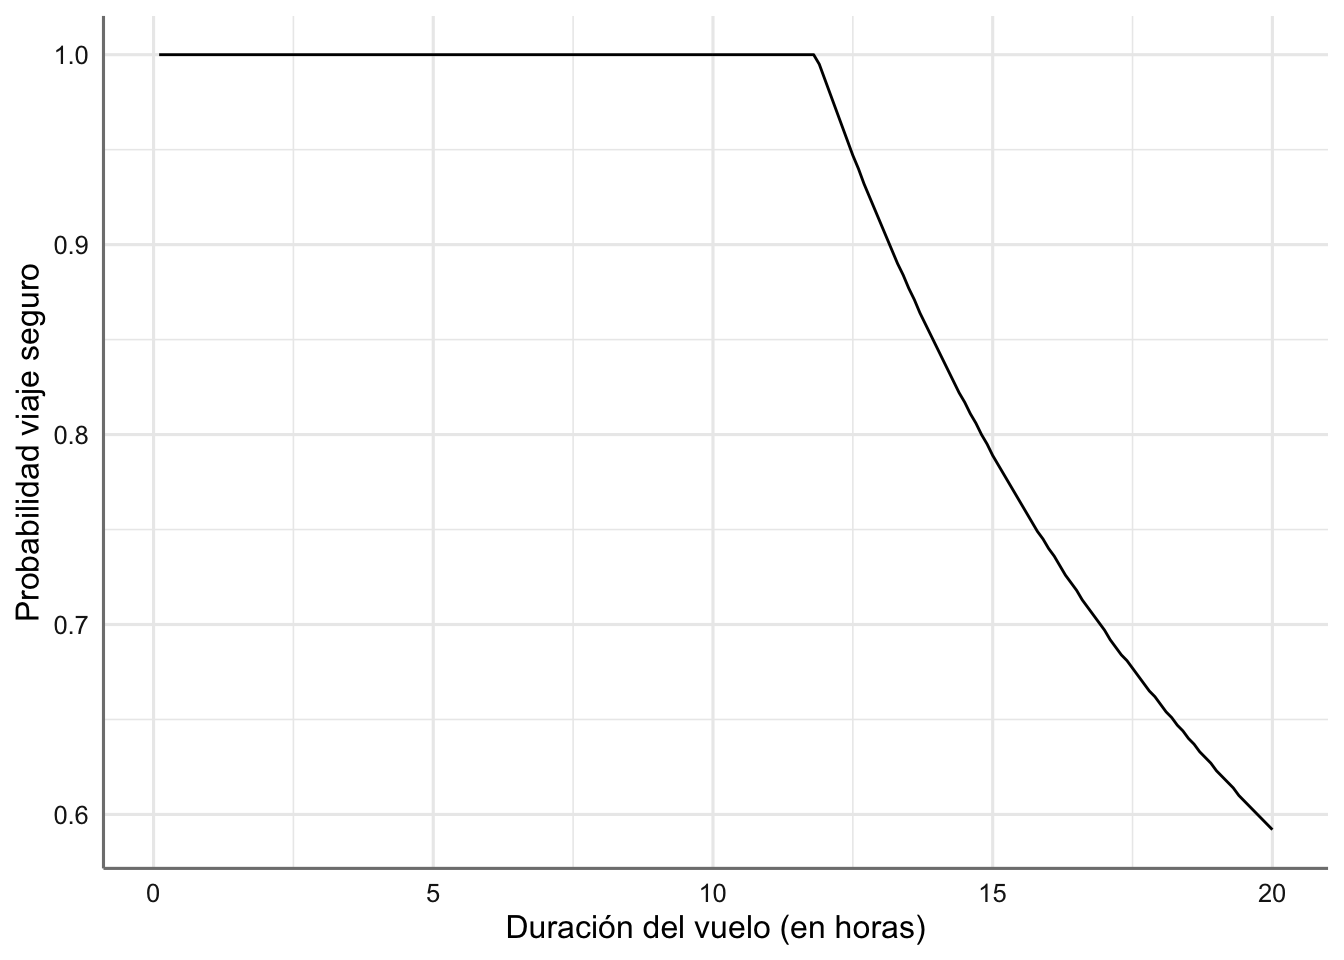
\includegraphics[width=0.95\linewidth]{04-CMTC_files/figure-latex/05-027-1} 

}

\caption{Probabilidad de un viaje seguro}\label{fig:05-027}
\end{figure}

\hypertarget{CMTCD}{%
\section{Procesos de nacimiento y muerte}\label{CMTCD}}

Los procesos de nacimiento y muerte que estudiamos en este apartado juegan un papel muy importante dentro de las CMTC, ya que son de uso habitual en muchas aplicaciones prácticas que veremos de ahora en adelante.

\begin{yellowbox}

\begin{definition}
\protect\hypertarget{def:cmtc002}{}\label{def:cmtc002}Una CMTC \(\{X_t; t \geq 0\}\) con espacio de estados \(S = \{0, 1, 2,...,N\}\) y matriz de tasas dada por:

\[R = 
\begin{pmatrix}
0 & \lambda_0 & 0 & 0 & \ldots & 0 & 0 \\
\mu_1 & 0 & \lambda_1 & 0 & \ldots & 0 & 0 \\
0 & \mu_2 & 0 & \lambda_2 & \ldots & 0 & 0 \\
\vdots & \vdots & \vdots & \vdots & \ldots & \vdots & \vdots \\
0 & 0 & 0 & 0 & \ldots & 0 & \lambda_{N-1} \\
0 & 0 & 0 & 0 & \ldots &\mu_N & 0
\end{pmatrix} \]

se denomina proceso finito de nacimiento y muerte donde los \(\lambda_i\) se denominan \textbf{parámetros de nacimiento} (transición del estado \(i\) al \(i+1\)) y los \(\mu_i\) se denominan \textbf{parámetros de muerte} (transición del estado \(i\) al \(i-1)\), donde por conveniencia se asume que \(\lambda_K = 0\) y \(\mu_0 = 0\) indicando que no hay nacimientos en el estado \(K\) y que no hay muertes en el estado \(0\).
\end{definition}

\end{yellowbox}

En esta situación el proceso permanece una cantidad de tiempo \(exp(\lambda_i + \mu_i)\) en el estado \(i\) y después salta al estado \(i+1\) con probabilidad \(\lambda_i/(\lambda_i + \mu_i)\), o al estado \(i-1\) con probabilidad \(\mu_i/(\lambda_i + \mu_i)\). Además, la matriz generadora del proceso viene dada por:

\[R = 
\begin{pmatrix}
- \lambda_0& \lambda_0 & 0 & 0 & \ldots & 0 & 0 \\
\mu_1 & -(\mu_1 + \lambda_1) & \lambda_1 & 0 & \ldots & 0 & 0 \\
0 & \mu_2 & -(\mu_2 + \lambda_2) & \lambda_2 & \ldots & 0 & 0 \\
\vdots & \vdots & \vdots & \vdots & \ldots & \vdots & \vdots \\
0 & 0 & 0 & 0 & \ldots & -(\mu_{k-1} + \lambda_{k-1}) & \lambda_{k-1} \\
0 & 0 & 0 & 0 & \ldots & \mu_k & -\mu_k
\end{pmatrix} \]

A continuación presentamos diferentes ejemplos de aplicación de los procesos de nacimiento y muerte.

\hypertarget{colas-de-espera-de-capacidad-finita-con-un-servidor}{%
\subsection{Colas de espera de capacidad finita con un servidor}\label{colas-de-espera-de-capacidad-finita-con-un-servidor}}

Aunque en la unidad siguiente estudiaremos con mucho más detalle los diferentes sistemas de colas de espera, vamos a presentar aquí el modelo más sencillo de colas, para comprobar que se puede modelar como un proceso de nacimiento y muerte.

Imaginemos que tenemos un cajero bancario al que los clientes acuden de acuerdo a Proceso de Poisson de parámetro \(\lambda\), es decir que las llegadas son aleatorias y se distribuyen según una \(Exp(\lambda)\). Si hay \(K-1\) clientes haciendo cola para ser atendidos, un cliente nuevo tomará la opción de buscar otro cajero, es decir, el sistema tiene capacidad \(K\) (1 cliente atendido y \(K-1\) en la cola de espera). Además, el tiempo de servicio del cajero tiene una distribución \(Exp(\mu)\).

En esta situación la variable \(X(t)\) que indica el número de sujetos en el sistema en el instante \(t\) es una CMTC denominada cola \(M/M/1/K\), donde \(M\) hace referencia a los tiempos de llegada y servicio exponenciales, el \(1\) hace referencia a la capacidad del servicio (sólo un cliente puede ser atendido en un instante dado), \(K\) es el tamaño del sistema (o aforo total), y \(S = \{0, 1, 2,...K \}\) el espacio de estados. Este tipo de sistemas son procesos de nacimiento y muerte con:

\begin{eqnarray*}
\lambda_i &=& \lambda, \quad 0 \leq i \leq K-1, \\
\mu_i &=& \mu, \quad 0 \leq i \leq K,
\end{eqnarray*}

donde el ``nacimiento'' y la ``muerte'' hacen referencia a la llegada al cajero y la salida del cajero respectivamente.

Veamos la descripción del sistema:

\begin{itemize}
\item
  En el estado \(X_t=0\) el sistema está vacío y el único evento que puede ocurrir es una llegada, que se produce después de un tiempo \(Exp(\lambda)\), provocando una transición al estado \(X_t=1\). En este caso \(r_{01} = \lambda\).
\item
  En el estado \(X_t=i\) (\(1 \leq i \leq K-1\)), tenemos dos posibilidades en el sistema: una llegada o una salida. En el primer caso tenemos \(r_{i, i+1} = \lambda\), mientras que en el segundo tenemos \(r_{i, i-1} = \mu\).
\item
  En el estado \(X_t=K\) sólo se puede producir una salida de forma que \(r_{K, K-1} = \mu\).
\end{itemize}

Por tanto, la matriz de tasas correspondiente a este proceso viene dada por:

\[R = 
\begin{pmatrix}
0 & \lambda & 0 & 0 & \ldots & 0 & 0 \\
\mu & 0 & \lambda & 0 & \ldots & 0 & 0 \\
0 & \mu & 0 & \lambda & \ldots & 0 & 0 \\
\vdots & \vdots & \vdots & \vdots & \ldots & \vdots & \vdots \\
0 & 0 & 0 & 0 & \ldots & 0 & \lambda \\
0 & 0 & 0 & 0 & \ldots &\mu & 0
\end{pmatrix} \]

El diagrama de tasas para una cola \(M/M/1/4\), es decir con una capacidad de 4 usuarios en el sistema (1 atendido y tres en espera) es:

\begin{figure}

{\centering 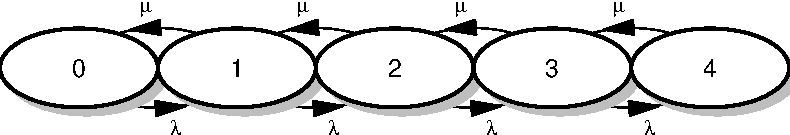
\includegraphics[width=0.95\linewidth]{04-CMTC_files/figure-latex/05-028-1} 

}

\caption{Diagrama de tasas para cola M/M/1/4.}\label{fig:05-028}
\end{figure}

Este sistema puede implementarse fácilmente en \texttt{simmer} si entendemos como ``resource'' al servicio del cajero y como ``generator'' la llegada al cajero. Escribimos el algoritmo de forma general para cualquier valor de \(K\).

\begin{Shaded}
\begin{Highlighting}[]
\CommentTok{\# Sistema}
\DocumentationTok{\#\#\#\#\#\#\#\#\#\#\#\#\#\#\#\#\#\#\#\#\#\#\#\#\#\#\#\#\#\#\#\#\#\#\#\#\#\#\#\#\#\#\#\#\#\#\#\#\#}
\NormalTok{cola.MM1K }\OtherTok{\textless{}{-}} \ControlFlowTok{function}\NormalTok{(t, lambda, mu, servidores, usuarios)}
\NormalTok{\{}
  \CommentTok{\# lambda: tasa de llegadas}
  \CommentTok{\# mu: tasa de servicio}
  \CommentTok{\# servidores: número de servidores}
  \CommentTok{\# usuarios: capacidad total del sistema}
\NormalTok{  cola }\OtherTok{\textless{}{-}}\NormalTok{ usuarios }\SpecialCharTok{{-}}\NormalTok{ servidores}
  
\NormalTok{  servicio }\OtherTok{\textless{}{-}} \FunctionTok{trajectory}\NormalTok{() }\SpecialCharTok{\%\textgreater{}\%}
    \CommentTok{\# empieza a ser atendido}
    \FunctionTok{seize}\NormalTok{(}\StringTok{"atendiendo"}\NormalTok{, }\AttributeTok{amount =} \DecValTok{1}\NormalTok{) }\SpecialCharTok{\%\textgreater{}\%}   
    \CommentTok{\# durante un tiempo exp(mu)}
    \FunctionTok{timeout}\NormalTok{(}\ControlFlowTok{function}\NormalTok{() }\FunctionTok{rexp}\NormalTok{(}\DecValTok{1}\NormalTok{, mu)) }\SpecialCharTok{\%\textgreater{}\%} 
    \CommentTok{\# termina el servicio de atención}
    \FunctionTok{release}\NormalTok{(}\StringTok{"atendiendo"}\NormalTok{, }\AttributeTok{amount =} \DecValTok{1}\NormalTok{)               }

  \CommentTok{\# Configuración del sistema }
  \DocumentationTok{\#\#\#\#\#\#\#\#\#\#\#\#\#\#\#\#\#\#\#\#\#\#\#\#\#\#\#\#\#\#\#\#\#\#\#\#\#\#\#\#\#\#\#\#\#\#\#\#\#}
  \FunctionTok{simmer}\NormalTok{() }\SpecialCharTok{\%\textgreater{}\%}
    \CommentTok{\# se crean los recursos (servidores) y se dimensiona la cola}
    \FunctionTok{add\_resource}\NormalTok{(}\StringTok{"atendiendo"}\NormalTok{, }\AttributeTok{capacity =}\NormalTok{ servidores, }\AttributeTok{queue\_size =}\NormalTok{ cola) }\SpecialCharTok{\%\textgreater{}\%}    
    \CommentTok{\# se generan las llegadas de clientes según Exp(lambda)}
    \FunctionTok{add\_generator}\NormalTok{(}\StringTok{"llegada"}\NormalTok{, servicio, }\ControlFlowTok{function}\NormalTok{() }\FunctionTok{rexp}\NormalTok{(}\DecValTok{1}\NormalTok{, lambda)) }\SpecialCharTok{\%\textgreater{}\%} 
    \FunctionTok{run}\NormalTok{(}\AttributeTok{until =}\NormalTok{ t)     }
\NormalTok{\}}
\end{Highlighting}
\end{Shaded}

Imaginemos que por la mañanas (de 8 a 15) las llegadas de clientes se producen con una tasa de 15 clientes/hora, mientras que el tiempo medio que el cliente permanece en el cajero es de 6 minutos. Expresada en minutos tendríamos una tasa de llegadas \(\lambda = 15/60\), y una tasa de servicio \(\mu = 1/6\). Se ha observado además que cuando la cola de espera es de tres clientes nadie más espera para hacer cola (\(K = 4\)). Analizamos el sistema de forma básica para una mañana cualquiera, es decir para un periodo de 7 horas (420 minutos).

\begin{Shaded}
\begin{Highlighting}[]
\FunctionTok{set.seed}\NormalTok{(}\DecValTok{12}\NormalTok{)}
\DocumentationTok{\#\#\# Simulación del sistema}
\NormalTok{t}\OtherTok{=}\DecValTok{420}\NormalTok{; }
\NormalTok{lambda}\OtherTok{=}\DecValTok{15}\SpecialCharTok{/}\DecValTok{60}\NormalTok{; mu}\OtherTok{=}\DecValTok{1}\SpecialCharTok{/}\DecValTok{6}
\NormalTok{servidores}\OtherTok{=}\DecValTok{1}\NormalTok{; usuarios}\OtherTok{=}\DecValTok{4}
\NormalTok{cajero }\OtherTok{\textless{}{-}} \FunctionTok{cola.MM1K}\NormalTok{(t, lambda, mu, servidores, usuarios)}
\DocumentationTok{\#\#\# Salidas del sistema}
\NormalTok{cajero.df.res }\OtherTok{\textless{}{-}} \FunctionTok{get\_mon\_resources}\NormalTok{(cajero)  }\CommentTok{\# recursos (servidores)}
\NormalTok{cajero.df.arr }\OtherTok{\textless{}{-}} \FunctionTok{get\_mon\_arrivals}\NormalTok{(cajero)   }\CommentTok{\# llegadas (clientes)}
\end{Highlighting}
\end{Shaded}

Veamos con un poco de detalle las salidas que proporciona el sistema. Comenzamos con el proceso de llegadas al sistema viendo las primeras 10 llegadas al sistema:

\begin{Shaded}
\begin{Highlighting}[]
\FunctionTok{head}\NormalTok{(cajero.df.arr, }\AttributeTok{n =} \DecValTok{10}\NormalTok{)}
\end{Highlighting}
\end{Shaded}

\begin{verbatim}
##         name start_time  end_time activity_time finished replication
## 1   llegada0   8.756865  9.461164      0.704299     TRUE           1
## 2   llegada1  11.299066 22.198513     10.899446     TRUE           1
## 3   llegada2  22.728061 46.307530     23.579469     TRUE           1
## 4   llegada7  53.191599 53.191599      0.000000    FALSE           1
## 5   llegada3  23.861384 53.496376      7.188846     TRUE           1
## 6   llegada9  57.528321 57.528321      0.000000    FALSE           1
## 7   llegada4  40.759227 59.558394      6.062018     TRUE           1
## 8  llegada11  68.130173 68.130173      0.000000    FALSE           1
## 9  llegada12  74.418248 74.418248      0.000000    FALSE           1
## 10  llegada5  45.814971 75.428935     15.870541     TRUE           1
\end{verbatim}

En la columna \texttt{name} tenemos el identificador de la llegada al sistema (cajero), en las columnas \texttt{start\_time} y \texttt{end\_time} tenemos el instante de tiempo en el que llega y sale del cajero. La columna \texttt{activity\_time} muestra el tiempo de servicio en el cajero (durante el que es atendido el cliente); un valor 0 identifica a un cliente que no ha sido atendido porque sobrepasó la capacidad del sistema (no esperó al ver la cola y se marchó). Estos coinciden con los valores \texttt{FALSE} de la columna \texttt{finished}, que identifica a los clientes que no han podido ser atendidos. Con estas salidas resulta muy fácil calcular el tiempo de servicio del sistema así como el porcentaje de clientes rechazados, y el tiempo esperando en la cola.

\begin{Shaded}
\begin{Highlighting}[]
\CommentTok{\# llegadas al sistema: número de clientes que han pasado por el cajero}
\NormalTok{nsis }\OtherTok{\textless{}{-}} \FunctionTok{nrow}\NormalTok{(cajero.df.arr);nsis}
\end{Highlighting}
\end{Shaded}

\begin{verbatim}
## [1] 108
\end{verbatim}

\begin{Shaded}
\begin{Highlighting}[]
\CommentTok{\# tiempo total de servicio}
\NormalTok{tserver }\OtherTok{\textless{}{-}} \FunctionTok{sum}\NormalTok{(cajero.df.arr}\SpecialCharTok{$}\NormalTok{activity\_time);tserver}
\end{Highlighting}
\end{Shaded}

\begin{verbatim}
## [1] 407.9837
\end{verbatim}

\begin{Shaded}
\begin{Highlighting}[]
\CommentTok{\# proporción de tiempo que el sistema está ocupado (atendiendo o en espera)}
\FunctionTok{round}\NormalTok{(}\DecValTok{100}\SpecialCharTok{*}\NormalTok{tserver}\SpecialCharTok{/}\NormalTok{t,}\DecValTok{2}\NormalTok{)}
\end{Highlighting}
\end{Shaded}

\begin{verbatim}
## [1] 97.14
\end{verbatim}

\begin{Shaded}
\begin{Highlighting}[]
\CommentTok{\# porcentaje de clientes que se marcharon sin ser atendidos}
\NormalTok{rechazados }\OtherTok{\textless{}{-}} \FunctionTok{sum}\NormalTok{(cajero.df.arr}\SpecialCharTok{$}\NormalTok{finished }\SpecialCharTok{==} \ConstantTok{FALSE}\NormalTok{)}
\FunctionTok{round}\NormalTok{(}\DecValTok{100}\SpecialCharTok{*}\NormalTok{rechazados}\SpecialCharTok{/}\NormalTok{nsis,}\DecValTok{2}\NormalTok{)}
\end{Highlighting}
\end{Shaded}

\begin{verbatim}
## [1] 48.15
\end{verbatim}

\begin{Shaded}
\begin{Highlighting}[]
\CommentTok{\# Tiempos de espera en cola para ser atendido}
\NormalTok{tespera }\OtherTok{\textless{}{-}}\NormalTok{ cajero.df.arr}\SpecialCharTok{$}\NormalTok{end\_time }\SpecialCharTok{{-}}\NormalTok{ cajero.df.arr}\SpecialCharTok{$}\NormalTok{start\_time }\SpecialCharTok{{-}}\NormalTok{ cajero.df.arr}\SpecialCharTok{$}\NormalTok{activity\_time}
\CommentTok{\# tiempo medio de espera en cola y desv.típica}
\FunctionTok{mean}\NormalTok{(tespera);}\FunctionTok{sd}\NormalTok{(tespera)}
\end{Highlighting}
\end{Shaded}

\begin{verbatim}
## [1] 8.280251
\end{verbatim}

\begin{verbatim}
## [1] 10.53434
\end{verbatim}

Podemos estudiar el comportamiento del sistema, y en particular de la cola, también en términos de los servidores.

\begin{Shaded}
\begin{Highlighting}[]
\FunctionTok{head}\NormalTok{(cajero.df.res, }\AttributeTok{n =} \DecValTok{10}\NormalTok{)}
\end{Highlighting}
\end{Shaded}

\begin{verbatim}
##      resource      time server queue capacity queue_size system limit replication
## 1  atendiendo  8.756865      1     0        1          3      1     4           1
## 2  atendiendo  9.461164      0     0        1          3      0     4           1
## 3  atendiendo 11.299066      1     0        1          3      1     4           1
## 4  atendiendo 22.198513      0     0        1          3      0     4           1
## 5  atendiendo 22.728061      1     0        1          3      1     4           1
## 6  atendiendo 23.861384      1     1        1          3      2     4           1
## 7  atendiendo 40.759227      1     2        1          3      3     4           1
## 8  atendiendo 45.814971      1     3        1          3      4     4           1
## 9  atendiendo 46.307530      1     2        1          3      3     4           1
## 10 atendiendo 48.326016      1     3        1          3      4     4           1
\end{verbatim}

En este caso las columnas nos informan sobre el instante de tiempo (\texttt{time}) en el que se produce alguna actividad en el sistema, la columna \texttt{server} indica el número de servidores ocupados atendiendo a algún cliente, \texttt{queue} el número de clientes en la cola de espera, \texttt{capacity} la capacidad de servicio del sistema, \texttt{queue\_size} el tamaño máximo de la cola, \texttt{system} el número de clientes en el sistema, \texttt{limit} la capacidad total de sistema, y finalmente \texttt{replication} da un indicador de la replicación de las simulaciones.

Con estas salidas podemos describir fácilmente el comportamiento de la cola del sistema ya que podemos estudiar el número de clientes en cola a lo largo del tiempo.

\begin{Shaded}
\begin{Highlighting}[]
\CommentTok{\# Evolución del tamaño de la cola}
\FunctionTok{ggplot}\NormalTok{(cajero.df.res, }\FunctionTok{aes}\NormalTok{(time, queue)) }\SpecialCharTok{+}
  \FunctionTok{geom\_step}\NormalTok{() }\SpecialCharTok{+}
  \FunctionTok{scale\_x\_continuous}\NormalTok{(}\AttributeTok{breaks =} \FunctionTok{seq}\NormalTok{(}\DecValTok{0}\NormalTok{, }\DecValTok{420}\NormalTok{, }\DecValTok{60}\NormalTok{)) }\SpecialCharTok{+} 
  \FunctionTok{labs}\NormalTok{(}\AttributeTok{x =} \StringTok{"Tiempo (en minutos)"}\NormalTok{, }\AttributeTok{y =} \StringTok{"Tamaño de la cola"}\NormalTok{)}
\end{Highlighting}
\end{Shaded}

\begin{center}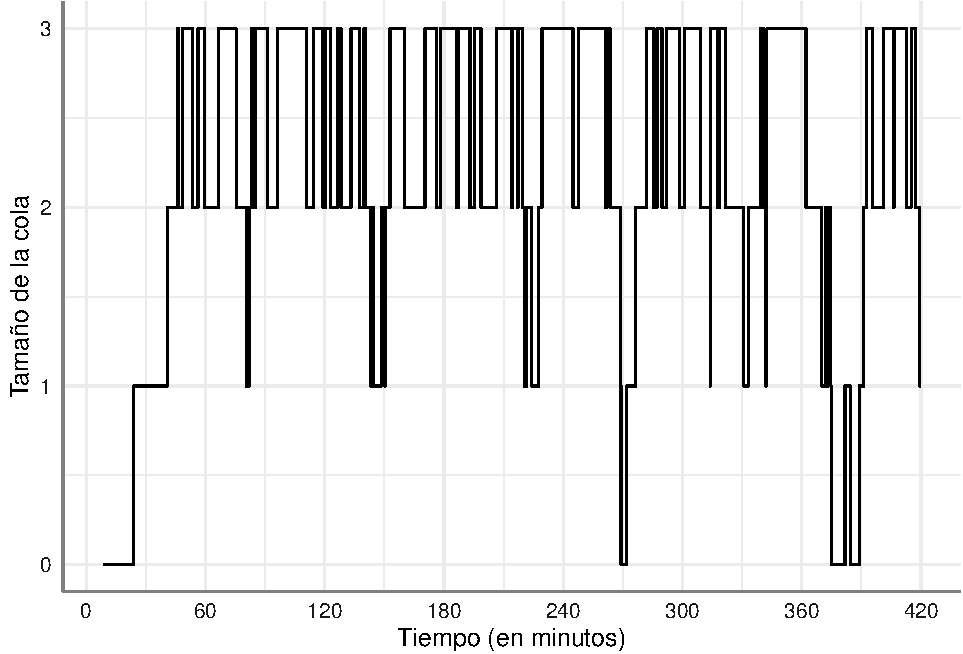
\includegraphics[width=0.95\linewidth]{04-CMTC_files/figure-latex/05-034-1} \end{center}

\begin{Shaded}
\begin{Highlighting}[]
\CommentTok{\# Porcentaje de clientes en cola}
\FunctionTok{ggplot}\NormalTok{(cajero.df.res, }\FunctionTok{aes}\NormalTok{(}\AttributeTok{x =}\NormalTok{ queue)) }\SpecialCharTok{+} 
  \FunctionTok{geom\_bar}\NormalTok{(}\FunctionTok{aes}\NormalTok{(}\AttributeTok{y =}\NormalTok{ ..prop.. , }\AttributeTok{group =} \DecValTok{1}\NormalTok{)) }\SpecialCharTok{+} 
  \FunctionTok{scale\_y\_continuous}\NormalTok{(}\AttributeTok{labels =}\NormalTok{ scales}\SpecialCharTok{::}\NormalTok{percent) }\SpecialCharTok{+} 
  \FunctionTok{labs}\NormalTok{(}\AttributeTok{x =} \StringTok{"Clientes en la cola"}\NormalTok{, }\AttributeTok{y =} \StringTok{"Porcentaje"}\NormalTok{)}
\end{Highlighting}
\end{Shaded}

\begin{center}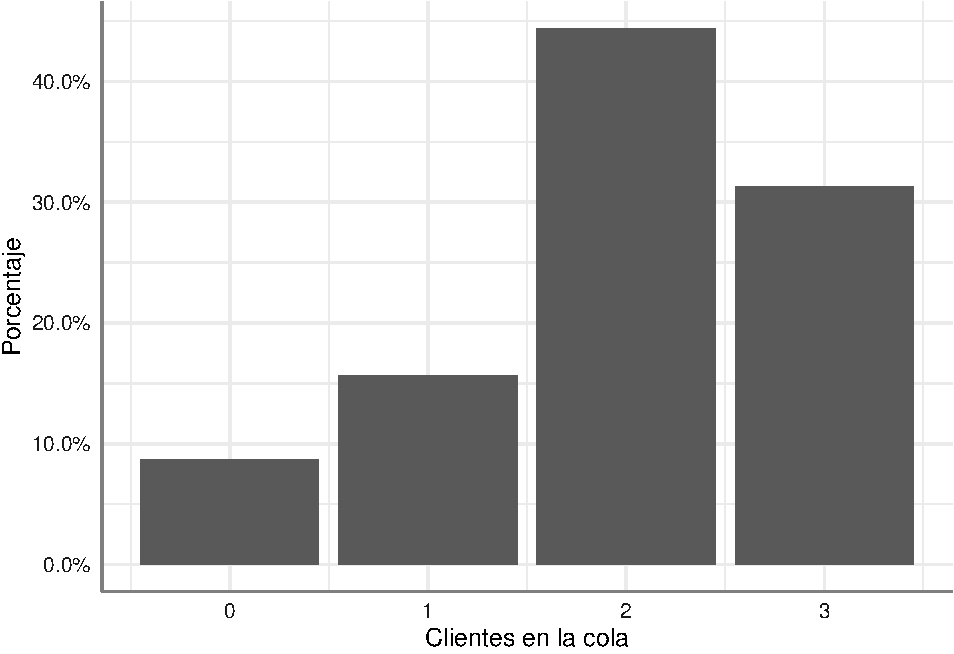
\includegraphics[width=0.95\linewidth]{04-CMTC_files/figure-latex/05-034-2} \end{center}

Simulamos ahora el sistema en 500 ocasiones para inferir con mayor precisión el comportamiento del sistema.

\begin{Shaded}
\begin{Highlighting}[]
\CommentTok{\# Réplicas del sistema}
\NormalTok{nreplicas}\OtherTok{=}\DecValTok{500}
\NormalTok{t}\OtherTok{=}\DecValTok{420}\NormalTok{; }
\NormalTok{lambda}\OtherTok{=}\DecValTok{15}\SpecialCharTok{/}\DecValTok{60}\NormalTok{; mu}\OtherTok{=}\DecValTok{1}\SpecialCharTok{/}\DecValTok{6}
\NormalTok{servidores}\OtherTok{=}\DecValTok{1}\NormalTok{; usuarios}\OtherTok{=}\DecValTok{4}

\NormalTok{envs }\OtherTok{\textless{}{-}} \FunctionTok{replicate}\NormalTok{(nreplicas,}\FunctionTok{cola.MM1K}\NormalTok{(t, lambda, mu, servidores, usuarios))}
\CommentTok{\# almacenamos análisis de llegadas del sistema}
\NormalTok{simarrivals}\OtherTok{\textless{}{-}}\FunctionTok{as\_tibble}\NormalTok{(}\FunctionTok{get\_mon\_arrivals}\NormalTok{(envs))}

\NormalTok{salida}\OtherTok{\textless{}{-}}\NormalTok{simarrivals }\SpecialCharTok{\%\textgreater{}\%} 
  \FunctionTok{group\_by}\NormalTok{(replication) }\SpecialCharTok{\%\textgreater{}\%} 
  \CommentTok{\# Resumen de las simualciones}
  \FunctionTok{summarise}\NormalTok{(}\AttributeTok{clientes =} \FunctionTok{n}\NormalTok{(), }
            \AttributeTok{tiemposervicio =} \FunctionTok{sum}\NormalTok{(activity\_time),}
            \AttributeTok{proptiemposervicio =} \FunctionTok{round}\NormalTok{(tiemposervicio}\SpecialCharTok{/}\DecValTok{420}\NormalTok{, }\DecValTok{2}\NormalTok{),}
            \AttributeTok{rechazados =}\NormalTok{ clientes }\SpecialCharTok{{-}} \FunctionTok{sum}\NormalTok{(finished),}
            \AttributeTok{proprechazados =} \FunctionTok{round}\NormalTok{(rechazados}\SpecialCharTok{/}\NormalTok{clientes,}\DecValTok{2}\NormalTok{)) }\SpecialCharTok{\%\textgreater{}\%} 
  \FunctionTok{summarise}\NormalTok{(}\AttributeTok{media\_clientes =} \FunctionTok{mean}\NormalTok{(clientes),}
            \AttributeTok{media\_tserver =} \FunctionTok{mean}\NormalTok{(tiemposervicio),}
            \AttributeTok{media\_ptserver =} \DecValTok{100}\SpecialCharTok{*}\FunctionTok{mean}\NormalTok{(proptiemposervicio),}
            \AttributeTok{media\_rechazados =} \FunctionTok{mean}\NormalTok{(rechazados),}
            \AttributeTok{media\_prechazados =} \DecValTok{100}\SpecialCharTok{*}\FunctionTok{mean}\NormalTok{(proprechazados)}
\NormalTok{            )}
\NormalTok{salida}
\end{Highlighting}
\end{Shaded}

\begin{verbatim}
## # A tibble: 1 x 5
##   media_clientes media_tserver media_ptserver media_rechazados media_prechazados
##            <dbl>         <dbl>          <dbl>            <dbl>             <dbl>
## 1           102.          377.           89.8             37.9              36.7
\end{verbatim}

\begin{quote}
Para comentar: ¿Qué conclusiones extraemos del análisis realizado? ¿Cómo valorarías la ocupación del sistema? ¿Qué ocurriría si añadimos un nuevo cajero y ampliamos la capacidad del sistema a 8 clientes?
\end{quote}

\hypertarget{excmtc007}{%
\subsection{Mantenimiento de máquinas}\label{excmtc007}}

El problema del mantenimiento de máquinas es muy habitual dentro de las CMTC. Supongamos que disponemos de \(N\) máquinas que funcionan durante 24 horas seguidas y \(M\) personas que pueden repararlas (\(M \leq N\)). Las máquinas son idénticas, y los tiempos de vida de las máquinas (reparaciones o mantenimiento) son variables aleatorias independientes \(Exp(\mu)\). Cuando las máquinas fallan, son reparadas por orden de fallo (la primera que falla es la primera en ser reparada) por los \(M\) reparadores. Cada máquina averiada necesita una y sólo una persona para repararla, y los tiempos de reparación se distribuyen como una \(Exp(\lambda)\); una vez reparada, la máquina continúa comportándose como una máquina nueva. Si \(X(t)\) el número de máquinas que funcionan en el momento \(t\), el proceso \(\{X(t), t \geq 0\}\) es un proceso de nacimiento (avería) y muerte (reparación) con parámetros:

\[\lambda_i = \lambda \cdot min(N-i, M), \quad 0 \leq i \leq N,\]

\[\mu_i = \mu \cdot i, \quad 0 \leq i \leq N.\]
::: example

Imaginemos un problema sencillo de mantenimiento de máquinas, que se puede generalizar fácilmente, en el que tenemos 4 máquinas y 2 reparadores, de forma que el espacio de estados (número de máquinas en funcionamiento) viene dado por \(S = \{0, 1, 2, 3, 4\}\). En este ejemplo vamos a ver cómo los parámetros de nacimiento y muerte corresponden con los que acabamos de definir.

:::

Descripción del sistema:

\begin{itemize}
\item
  En el estado \(X(t)=0\), todas las máquinas están estropeadas, dos se encuentran en reparación (puesto que hay dos reparadores) y dos esperando a ser reparadas, Los tiempos de reparación son iid \(Exp(\lambda)\) y un vez se complete cualquiera de las dos repaciones el sistema cambiará al estado 1. De esta forma, \(r_{01} = \lambda_0 = \lambda + \lambda = 2\lambda\).
\item
  En el estado \(X(t)=1\), una máquina está en funcionamiento, hay dos en reparación y otra está en espera. Cuando una de las dos máquinas es reparada pasamos al estado 2. De esta forma, \(r_{12} = \lambda_1 = 2\lambda\). Además, en este estado la máquina que está funcionando puede fallar después de mantenerse en funcionamiento un tiempo \(Exp(\mu)\) volviendo al estado 0, de forma que, \(r_{10} = \mu_1 = \mu\).
\item
  En el estado \(X(t)=2\), con razonamientos similares, tendremos que \(r_{23} = \lambda_2 = 2\lambda\) y \(r_{21} = \mu_2 = 2\mu\).
\item
  Para el resto de estados tendremos que \(r_{34} = \lambda_3 = \lambda\), \(r_{32} = mu_3 = 3\mu\), y \(r_{43} = \mu_4 = 4\mu\).
\end{itemize}

En esta situación el diagrama del proceso viene dado por:

\begin{figure}

{\centering 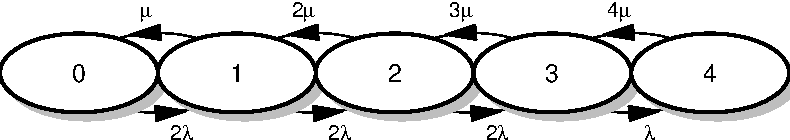
\includegraphics[width=0.95\linewidth]{04-CMTC_files/figure-latex/05-036-1} 

}

\caption{Diagrama de tasas para el mantenimiento de máquinas}\label{fig:05-036}
\end{figure}

Este sistema se puede modelizar fácilmente en \texttt{simmer} sin más que fijar las tasas correspondientes, el número de máquinas disponibles, y el número de operarios. Supongamos que los tiempos de vida de las máquinas son variables aleatorias exponenciales con media de 3 días, mientras que los tiempos de reparación son variables exponenciales con media de 2 horas. Expresando todo en horas, tendríamos una tasa de reparación de \(\mu = 1/2\), y una tasa de llegadas \(\lambda = 1/72\).

De nuevo planteamos una función que nos permita cambiar fácilmente los parámetros del sistema si fuera necesario. La empresa está interesada en:

\begin{itemize}
\tightlist
\item
  ¿Cuántas máquinas estarán en funcionamiento después de 3 días?
\item
  ¿Durante qué porcentaje del tiempo las cuatro máquinas están funcionando?
\end{itemize}

\begin{Shaded}
\begin{Highlighting}[]
\CommentTok{\# Sistema}
\DocumentationTok{\#\#\#\#\#\#\#\#\#\#\#\#\#\#\#\#\#\#\#\#\#\#\#\#\#\#\#\#\#\#\#\#\#\#\#\#\#\#\#\#\#\#\#\#\#\#\#\#\#}
\NormalTok{mantenimiento }\OtherTok{\textless{}{-}} \ControlFlowTok{function}\NormalTok{(t, lambda, mu, capacidad)}
\NormalTok{\{}
  \CommentTok{\# lambda: tasa de reparación}
  \CommentTok{\# mu: tasa de vida de la máquina}
  \CommentTok{\# capacidad: reparadores}
  \CommentTok{\# K: máquinas}
  
  \CommentTok{\# Distribuciones de tiempos}
\NormalTok{  vida }\OtherTok{\textless{}{-}} \ControlFlowTok{function}\NormalTok{() }\FunctionTok{rexp}\NormalTok{(}\DecValTok{1}\NormalTok{, lambda)}
\NormalTok{  reparacion }\OtherTok{\textless{}{-}} \ControlFlowTok{function}\NormalTok{() }\FunctionTok{rexp}\NormalTok{(}\DecValTok{1}\NormalTok{, mu)}
  
  \CommentTok{\# Trayectoria }
\NormalTok{  maquina }\OtherTok{\textless{}{-}} \FunctionTok{trajectory}\NormalTok{() }\SpecialCharTok{\%\textgreater{}\%}
    \FunctionTok{seize}\NormalTok{(}\StringTok{"funcionando"}\NormalTok{) }\SpecialCharTok{\%\textgreater{}\%}
    \FunctionTok{timeout}\NormalTok{(vida) }\SpecialCharTok{\%\textgreater{}\%}
    \FunctionTok{release}\NormalTok{(}\StringTok{"funcionando"}\NormalTok{) }\SpecialCharTok{\%\textgreater{}\%}
    \FunctionTok{seize}\NormalTok{(}\StringTok{"reparando"}\NormalTok{) }\SpecialCharTok{\%\textgreater{}\%}
    \FunctionTok{timeout}\NormalTok{(reparacion) }\SpecialCharTok{\%\textgreater{}\%}
    \FunctionTok{release}\NormalTok{(}\StringTok{"reparando"}\NormalTok{) }\SpecialCharTok{\%\textgreater{}\%}    
    \FunctionTok{rollback}\NormalTok{(}\DecValTok{6}\NormalTok{)}

  \CommentTok{\# Configuración del sistema }
  \FunctionTok{simmer}\NormalTok{() }\SpecialCharTok{\%\textgreater{}\%}
    \FunctionTok{add\_resource}\NormalTok{(}\StringTok{"funcionando"}\NormalTok{, }\AttributeTok{capacity =} \ConstantTok{Inf}\NormalTok{) }\SpecialCharTok{\%\textgreater{}\%}
    \FunctionTok{add\_resource}\NormalTok{(}\StringTok{"reparando"}\NormalTok{, }\AttributeTok{capacity =}\NormalTok{ capacidad, }\AttributeTok{queue\_size =} \ConstantTok{Inf}\NormalTok{) }\SpecialCharTok{\%\textgreater{}\%}
    \FunctionTok{add\_generator}\NormalTok{(}\StringTok{"sistema"}\NormalTok{, maquina, }\FunctionTok{at}\NormalTok{(}\DecValTok{0}\NormalTok{, }\DecValTok{0}\NormalTok{, }\DecValTok{0}\NormalTok{, }\DecValTok{0}\NormalTok{)) }\SpecialCharTok{\%\textgreater{}\%}
    \FunctionTok{run}\NormalTok{(}\AttributeTok{until =}\NormalTok{ t)     }
\NormalTok{\}}
\end{Highlighting}
\end{Shaded}

Simulamos el sistema y analizamos un poco la salida. Dado que en este sistema no hay llegadas solo podemos estudiar los recursos.

\begin{Shaded}
\begin{Highlighting}[]
\NormalTok{t}\OtherTok{=}\DecValTok{72} \CommentTok{\# 3 días}
\NormalTok{lambda}\OtherTok{=}\DecValTok{1}\SpecialCharTok{/}\DecValTok{72}\NormalTok{; mu}\OtherTok{=}\DecValTok{1}\SpecialCharTok{/}\DecValTok{2}
\NormalTok{capacidad}\OtherTok{=}\DecValTok{2} \CommentTok{\# nº reparadores}
\DocumentationTok{\#\#\# Simulación del sistema}
\NormalTok{maquinas }\OtherTok{\textless{}{-}} \FunctionTok{mantenimiento}\NormalTok{(t, lambda,mu, capacidad)}
\DocumentationTok{\#\#\# Salidas del sistema}
\NormalTok{maquinas.df.res }\OtherTok{\textless{}{-}} \FunctionTok{get\_mon\_resources}\NormalTok{(maquinas)}
\FunctionTok{head}\NormalTok{(maquinas.df.res, }\DecValTok{10}\NormalTok{)}
\end{Highlighting}
\end{Shaded}

\begin{verbatim}
##       resource     time server queue capacity queue_size system limit replication
## 1  funcionando  0.00000      1     0      Inf        Inf      1   Inf           1
## 2  funcionando  0.00000      2     0      Inf        Inf      2   Inf           1
## 3  funcionando  0.00000      3     0      Inf        Inf      3   Inf           1
## 4  funcionando  0.00000      4     0      Inf        Inf      4   Inf           1
## 5  funcionando 39.64840      3     0      Inf        Inf      3   Inf           1
## 6    reparando 39.64840      1     0        2        Inf      1   Inf           1
## 7    reparando 40.91384      0     0        2        Inf      0   Inf           1
## 8  funcionando 40.91384      4     0      Inf        Inf      4   Inf           1
## 9  funcionando 63.84362      3     0      Inf        Inf      3   Inf           1
## 10   reparando 63.84362      1     0        2        Inf      1   Inf           1
\end{verbatim}

Respondemos en primer lugar al número de máquinas en funcionamiento a los tres días

\begin{Shaded}
\begin{Highlighting}[]
\CommentTok{\# última iteración del sistema}
\FunctionTok{tail}\NormalTok{(maquinas.df.res, }\DecValTok{1}\NormalTok{)}
\end{Highlighting}
\end{Shaded}

\begin{verbatim}
##       resource     time server queue capacity queue_size system limit replication
## 12 funcionando 65.62617      4     0      Inf        Inf      4   Inf           1
\end{verbatim}

A las 72 horas el número de máquinas funcionando se corresponde con el valor de \texttt{server}. Para conocer el tiempo que las cuatro máquinas han estado funcionando debemos manipular los resultados obtenidos en el proceso de simulación.

\begin{Shaded}
\begin{Highlighting}[]
\DocumentationTok{\#\#\# Seleccionamos todos los recursos cuando las máquinas están funcionando}
\NormalTok{maquinas.df.sel }\OtherTok{\textless{}{-}}\NormalTok{ maquinas.df.res }\SpecialCharTok{\%\textgreater{}\%}
  \FunctionTok{subset}\NormalTok{(resource }\SpecialCharTok{==} \StringTok{"funcionando"}\NormalTok{)}
\DocumentationTok{\#\#\# Calculamos los tiempos de funcionamiento}
\NormalTok{deltas\_4 }\OtherTok{\textless{}{-}} \FunctionTok{diff}\NormalTok{(maquinas.df.sel}\SpecialCharTok{$}\NormalTok{time)}
\DocumentationTok{\#\#\# Seleccionamos cuando las 4 máquinas están activas}
\NormalTok{both\_working\_4 }\OtherTok{\textless{}{-}} \FunctionTok{which}\NormalTok{(maquinas.df.sel}\SpecialCharTok{$}\NormalTok{system }\SpecialCharTok{==} \DecValTok{4}\NormalTok{)}
\NormalTok{t\_both\_working\_4 }\OtherTok{\textless{}{-}}\NormalTok{ deltas\_4[both\_working\_4]}
\DocumentationTok{\#\#\# Caculamos la proporción de tiempo}
\NormalTok{res}\OtherTok{\textless{}{-}}\FunctionTok{sum}\NormalTok{(t\_both\_working\_4, }\AttributeTok{na.rm=}\ConstantTok{TRUE}\NormalTok{) }\SpecialCharTok{/} \FunctionTok{max}\NormalTok{(maquinas.df.sel}\SpecialCharTok{$}\NormalTok{time)}
\end{Highlighting}
\end{Shaded}

La proporción de tiempo en que las cuatro máquinas están funcionando simultáneamente es 95.36. Estudiamos la estabilidad del sistema realizando 500 simulaciones del sistema y estimando las cantidades de interés para la empresa.

\begin{Shaded}
\begin{Highlighting}[]
\CommentTok{\# Réplicas del sistema}
\NormalTok{replicas }\OtherTok{\textless{}{-}} \DecValTok{500}
\NormalTok{envs }\OtherTok{\textless{}{-}} \FunctionTok{lapply}\NormalTok{(}\DecValTok{1}\SpecialCharTok{:}\NormalTok{replicas, }\ControlFlowTok{function}\NormalTok{(i)\{}
\NormalTok{  maquinas }\OtherTok{\textless{}{-}} \FunctionTok{mantenimiento}\NormalTok{(}\DecValTok{72}\NormalTok{, }\DecValTok{1}\SpecialCharTok{/}\DecValTok{2}\NormalTok{, }\DecValTok{1}\SpecialCharTok{/}\DecValTok{72}\NormalTok{, }\DecValTok{2}\NormalTok{)}
\NormalTok{\})}

\CommentTok{\# almacenamos análisis de llegadas del sistema}
\NormalTok{simresources}\OtherTok{\textless{}{-}}\FunctionTok{as\_tibble}\NormalTok{(}\FunctionTok{get\_mon\_resources}\NormalTok{(envs))}
\DocumentationTok{\#\# funciones para calcular cantidades de interés}
\NormalTok{maquinasON }\OtherTok{\textless{}{-}} \FunctionTok{vector}\NormalTok{()}
\NormalTok{propTimeON }\OtherTok{\textless{}{-}} \FunctionTok{vector}\NormalTok{()}
\ControlFlowTok{for}\NormalTok{ (i }\ControlFlowTok{in} \DecValTok{1}\SpecialCharTok{:}\DecValTok{500}\NormalTok{)}
\NormalTok{\{}
\NormalTok{  datos }\OtherTok{\textless{}{-}}\NormalTok{ simresources[simresources}\SpecialCharTok{$}\NormalTok{replication }\SpecialCharTok{==}\NormalTok{ i,]}
  \CommentTok{\# máquinas en funcionamiento}
\NormalTok{  maquinasON[i] }\OtherTok{\textless{}{-}} \FunctionTok{tail}\NormalTok{(datos, }\DecValTok{1}\NormalTok{)}\SpecialCharTok{$}\NormalTok{server}
  \CommentTok{\# Proporción de tiempo}
\NormalTok{  maquinas.df.sel }\OtherTok{\textless{}{-}}\NormalTok{ datos }\SpecialCharTok{\%\textgreater{}\%}
  \FunctionTok{subset}\NormalTok{(resource }\SpecialCharTok{==} \StringTok{"funcionando"}\NormalTok{)}
  \DocumentationTok{\#\#\# Calculamos los tiempos de funcionamiento}
\NormalTok{  deltas\_4 }\OtherTok{\textless{}{-}} \FunctionTok{diff}\NormalTok{(maquinas.df.sel}\SpecialCharTok{$}\NormalTok{time)}
  \DocumentationTok{\#\#\# Seleccionamos cuando las 4 máquinas están activas}
\NormalTok{  both\_working\_4 }\OtherTok{\textless{}{-}} \FunctionTok{which}\NormalTok{(maquinas.df.sel}\SpecialCharTok{$}\NormalTok{system }\SpecialCharTok{==} \DecValTok{4}\NormalTok{)}
\NormalTok{  t\_both\_working\_4 }\OtherTok{\textless{}{-}}\NormalTok{ deltas\_4[both\_working\_4]}
  \DocumentationTok{\#\#\# Caculamos la proporción de tiempo}
\NormalTok{  propTimeON[i]}\OtherTok{\textless{}{-}}\FunctionTok{round}\NormalTok{(}\DecValTok{100}\SpecialCharTok{*}\FunctionTok{sum}\NormalTok{(t\_both\_working\_4, }\AttributeTok{na.rm=}\ConstantTok{TRUE}\NormalTok{) }\SpecialCharTok{/} \FunctionTok{max}\NormalTok{(maquinas.df.sel}\SpecialCharTok{$}\NormalTok{time), }\DecValTok{2}\NormalTok{)}
\NormalTok{\}}
\end{Highlighting}
\end{Shaded}

Tenemos entonces que el número de máquinas en funcionamiento es 1.97 y el tiempo de funcionamiento de las cuatro máquinas estimado es 3.58 para un periodo de 72 horas cuando al inicio todas las máquinas están paradas.

\hypertarget{central-telefuxf3nica}{%
\subsection{Central telefónica}\label{central-telefuxf3nica}}

Una centralita telefónica puede atender \(K\) llamadas a la vez en un momento dado. Las llamadas llegan según un proceso de Poisson con tasa \(\lambda\). Si la centralita ya está atendiendo \(K\) llamadas cuando llega una nueva llamada, ésta se pierde. Si una llamada es aceptada, dura un tiempo \(Exp(\mu)\) y luego termina. Todas las llamadas son independientes entre sí. Sea \(X(t)\) el número de llamadas que la centralita gestiona en el momento \(t\).

El proceso \(\{X(t); t \geq 0\}\) es una CMTC con espacio de estados \(S = \{0, 1, 2,...,K\}\) de forma que:

\begin{itemize}
\item
  En el estado \(i\), con \(0 \leq i \leq K-1\) la llegada de una llamada desencadena una transición al estado \(i+1\) con tasa \(\lambda\) (\(r_{i i+1} = \lambda\)), mientras que en el estado \(K\) no se pueden recibir llamadas.
\item
  En el estado \(i\), con \(1 \leq i \leq K\) cualquiera de las llamadas \(i\) puede completarse y desancedar una transición al estado \(i-1\). La tasa de transición es \(r_{i i-1} = i\mu\). En el estado 0 no hay salidas.
\end{itemize}

El sistema \(\{X(t); t \geq 0\}\) es un proceso de nacimiento y muerte con:

\[\lambda_i = \lambda, \quad 0 \leq i \leq K-1\] \[\mu_i = i\mu, \quad 0 \leq i \leq K\] que como veremos más adelante se denomina cola \(M/M/K/K\), es decir, llegadas y servicios exponenciales con \(K\) servidores y de capacidad \(K\).

La función de simmer para estudiar este sistema viene dada por:

\begin{Shaded}
\begin{Highlighting}[]
\CommentTok{\# Sistema}
\DocumentationTok{\#\#\#\#\#\#\#\#\#\#\#\#\#\#\#\#\#\#\#\#\#\#\#\#\#\#\#\#\#\#\#\#\#\#\#\#\#\#\#\#\#\#\#\#\#\#\#\#\#}
\NormalTok{cola.MMKK }\OtherTok{\textless{}{-}} \ControlFlowTok{function}\NormalTok{(t, lambda, mu, servidores, usuarios)}
\NormalTok{\{}
  \CommentTok{\# lambda: tasa de llegadas}
  \CommentTok{\# mu: tasa de servicio}
  \CommentTok{\# servidores: número de servidores}
  \CommentTok{\# usuarios: capacidad total del sistema}
\NormalTok{  cola }\OtherTok{\textless{}{-}}\NormalTok{ usuarios }\SpecialCharTok{{-}}\NormalTok{ servidores}
  
\NormalTok{  servicio }\OtherTok{\textless{}{-}} \FunctionTok{trajectory}\NormalTok{() }\SpecialCharTok{\%\textgreater{}\%}
    \FunctionTok{seize}\NormalTok{(}\StringTok{"atendiendo"}\NormalTok{, }\AttributeTok{amount =} \DecValTok{1}\NormalTok{) }\SpecialCharTok{\%\textgreater{}\%}              
    \FunctionTok{timeout}\NormalTok{(}\ControlFlowTok{function}\NormalTok{() }\FunctionTok{rexp}\NormalTok{(}\DecValTok{1}\NormalTok{, mu)) }\SpecialCharTok{\%\textgreater{}\%}   
    \FunctionTok{release}\NormalTok{(}\StringTok{"atendiendo"}\NormalTok{, }\AttributeTok{amount =} \DecValTok{1}\NormalTok{)               }

  \CommentTok{\# Configuración del sistema }
  \DocumentationTok{\#\#\#\#\#\#\#\#\#\#\#\#\#\#\#\#\#\#\#\#\#\#\#\#\#\#\#\#\#\#\#\#\#\#\#\#\#\#\#\#\#\#\#\#\#\#\#\#\#}
  \FunctionTok{simmer}\NormalTok{() }\SpecialCharTok{\%\textgreater{}\%}
    \FunctionTok{add\_resource}\NormalTok{(}\StringTok{"atendiendo"}\NormalTok{, }\AttributeTok{capacity =}\NormalTok{ servidores, }\AttributeTok{queue\_size =}\NormalTok{ cola) }\SpecialCharTok{\%\textgreater{}\%}           
    \FunctionTok{add\_generator}\NormalTok{(}\StringTok{"llegada"}\NormalTok{, servicio, }\ControlFlowTok{function}\NormalTok{() }\FunctionTok{rexp}\NormalTok{(}\DecValTok{1}\NormalTok{, lambda)) }\SpecialCharTok{\%\textgreater{}\%} 
    \FunctionTok{run}\NormalTok{(}\AttributeTok{until =}\NormalTok{ t)     }
\NormalTok{\}}
\end{Highlighting}
\end{Shaded}

\hypertarget{call-center}{%
\subsection{Call Center}\label{call-center}}

El sistema de reservas telefónicas de una aerolínea es un ``call center'' formado por \(s\) empleados de reservas llamados agentes. Una llamada entrante para una reserva es atendida por un agente si hay uno disponible; de lo contrario, la persona que llama es puesta en espera. El sistema puede poner en espera a un máximo de \(H\) personas. Cuando un agente está disponible, las llamadas en espera se atienden por orden de llegada. Cuando todos los agentes están ocupados y hay \(H\) llamadas en espera, cualquier llamada adicional recibe una señal de ocupado y se pierden permanentemente. Sea \(X(t)\) la varaible aleatoria que registra el número de llamadas en el sistema, las atendidas por los agentes más las que están en espera, en el momento \(t\) . Si las llamadas recibidas se comportan como un \(PP(\lambda)\) y los tiempos de procesamiento de las llamadas son variables aleatorias iid \(Exp(\mu)\), el sistema \(\{X(t); t \geq 0\}\) es una CMTC, con espacio de estados \(S = \{0, 1, 2,...,K\}\) donde \(K = s + H\).

Se puede demostrar fácilmente que este sistema es un proceso de nacimiento y muerte con tasas:

\[\lambda_i = \lambda, \quad 0 \leq i \leq K-1\] \[\mu_i = min(i, s)\mu, \quad 0 \leq i \leq K\] que en la terminologia habitual se denomina cola \(M/M/s/K\). Para simular este proceso podemos utilizar la función del ejemplo anterior.

\hypertarget{CMTCE}{%
\section{Otros tipos de sistemas}\label{CMTCE}}

Presentamos en este punto otros sistemas que no se corresponden con procesos de nacimiento y muerte, pero que son muy habituales en el mundo real.

\hypertarget{gestiuxf3n-de-inventarios}{%
\subsection{Gestión de inventarios}\label{gestiuxf3n-de-inventarios}}

Una tienda minorista gestiona el inventario de un tipo de producto, que denominamos \(P\), de la forma siguiente. Cuando el número de elementos de \(P\) disminuye a un número fijo \(l\), se hace un pedido al fabricante de \(m\) repuestos de \(P\). El pedido tarda un tiempo aleatorio en ser entregado al minorista. Si el inventario es como máximo \(l\) cuando se entrega un pedido (incluido el pedido recién entregado), se realiza inmediatamente otro pedido de \(m\) artículos. Supongamos que que los plazos de entrega son variables aleatorias iid \(Exp(\lambda)\) y que la demanda se produce según un \(PP(\mu)\). Las demandas que no pueden ser satisfechas inmediatamente se pierden.

Sea \(X(t)\) el número de elementos de \(P\) en stock en el momento \(t\). Obsérvese que el número máximo de elemntos de \(P\) en stock es \(K = l + m\), lo que ocurre si el pedido se entrega antes de que se produzca la siguiente demanda. El espacio de estados es, pues, \(S = \{0, 1, 2,...,K\}\). En el estado \(0\), las demandas se pierden, y el stock salta a \(m\) cuando se entrega el pedido pendiente actual (lo que ocurre a la tasa \(\lambda\)). Por tanto, tenemos \(r_{0m} = \lambda\). En el estado \(i\) \((1 \leq i \leq l)\) hay un pedido pendiente. El estado cambia a \(i-1\) si se produce una demanda (lo que ocurre a la tasa \(\mu\)) y a \(i + m\) si se entrega el pedido. Por lo tanto, tenemos \(r_{i i+m} = \lambda\) y \(r_{i i-1} = \mu\). Finalmente, si \(X(t) = i\) (\(l + 1 \leq i \ K\)), no hay pedidos pendientes, y la única transición es de \(i\) a \(i- 1\), y eso ocurre cuando se produce una demanda. Por lo tanto, \(r_{i i-1} = \mu\). El proceso \(X(t), t \geq 0\) definidido de esta forma es una CMTC.

Consulta sobre modelo simmer para inventarios (\url{https://stackoverflow.com/questions/51680140/immediate-inventory-restock-in-r-simmer})

\hypertarget{proceso-de-fabricaciuxf3n}{%
\subsection{Proceso de fabricación}\label{proceso-de-fabricaciuxf3n}}

Un proceso de de fabricación sencilla consiste en una sola máquina que puede estar encendida o apagada. Si la máquina está encendida, produce artículos según un proceso de Poisson con tasa \(\lambda\). La demanda de artículos llega según un \(PP(\mu)\) La máquina se controla de la siguiente manera. Si el número de artículos en stock alcanza un número máximo \(K\) (la capacidad de almacenamiento), la máquina se apaga. La máquina se enciende cuando el número de artículos en stock disminuye hasta un nivel preestablecido \(l < K\). Si la variable aleatoria \(X(t)\) nos indica el número de artículos en stock en el momento \(t\), el proceso \(X(t), t \geq 0\) no es una CMTC ya que no sabemos si la máquina está encendida o apagada si \(l < X(t) < K\). Si se considera \(Y(t)\) como el estado en el que se encuentra la máquina en el momento \(t\), de forma que un \(1\) indica encendido y un \(0\) que está apagada, entonces el proceso \(\{X(t), Y(t), t\geq 0\}\) es una CMTC con espacio de estados:

\[S = \{(i, 1), 0 \leq i < K\} \cup \{(i, 0), l < i \leq K\}\]

Hay que tener en cuenta que la máquina siempre está encendida si el número de elementos es \(l\) o menos. Por lo tanto, no necesitamos los estados \(\{(i, 0), 0 \leq i \leq l\}\). El análisis habitual de los eventos desencadenantes arroja las siguientes tasas de transición:

\[r_{(i, 1)(i+1, 1)} = \lambda, \quad 0 \leq i < K-1,\]

\[r_{(K-1, 1)(K, 0)} = \lambda, \] \[r_{(i, 1)(i-1, 1)} = \mu, \quad 1\leq i\leq K-1,\]

\[r_{(i, 0)(i-1, 0)} = \mu, \quad l+1 < i\leq K,\]

\[r_{(l+1, 0)(l, 1)} = \mu.\]

\hypertarget{CMTCF}{%
\section{Probabilidades de transición}\label{CMTCF}}

El aspecto funcdamental para estudiar el comportamiento de cualquier CMTC es la obtención y análisis de las probabilidades de transición entre los estados del procso a partir de la matriz de tasas obtenida en puntos anteriores. Aunque haremos un desarrollo teórico de este rporblema, veremos que es necesario un algoritmo de computación para obtener dichas probabilidades.

Sea \(X(t), t \geq 0\) una CMTC con espacio de estados \(S = \{1,2,...,N\}\) y con matriz de tasas \(R = [r_{ij}]\). Si asumimos que la distribución de probabilidad en el estado incial, \(X(0)\) es conocida, entonces tenemos que:

\[P(X(t) = j) = \sum_{i=1}^N P(X(t) = j | X_0 = i)P(X_0 = i), \quad 1 \leq j \leq N.\] Es necesario obtener \(P(X(t) = j | X_0 = i) = p_{ij}(t)\) para obtener la función de distribución de probabilidad de \(X(t)\). Antes de ver como obtener dichas probabildiades introducimos la notación necesaria.

ya hemos visto antes que una CMTC permance un tiempo \(Exp(r_i)\) en el estado \(i\) con \(r_i = \sum_{j=1}^N r_{ij}\) y, si \(r_i > 0\) entonces pasamos al estado \(j\) con probabilidad \(p_{ij} = r_{ij}/r_i\). Asumiendo que existe un número finito \(r\) que satisface:

\[r \geq max(r_i), \quad 1\leq i \leq N\] podemos definir la matriz \(\hat{P} = [\hat{p}_{ij}]\) como:

\begin{equation}
\hat{p}_{ij} = 
\begin{cases} 
1-\frac{r_i/r} & \text{ si } i=j\\
r_{ij}/r & \text{ si } i \neq j
\end{cases}
\end{equation}

que es una matriz estocástica.

\begin{theorem}
La matriz de tarnsición de probabilidades, \(P\), de una CMTC viene dada por:

\[P(t) = \sum_{k=0}^{\infty} e^{-rt}\frac{(rt)^k}{k!} \hat{P}^k\]
\end{theorem}

Esta forma de obtener \(P\) se denomina \textbf{método de uniformización}, y proporciona un método numérico para obtener las probabilidades de transición deseadas, sin más que usar los \(m\) primeros términos de la serie infinita definida. Para asegurar la convergencia de dichas probabilidades se usan como reglas habituales:

\[m \approx max\{rt + r\sqrt{rt}, 20\},\]

y

\[r = max(r_i), \quad 1\leq i \leq N,\] aunque en algunos casos resulta más conveniente utilizar \(r = sum_{i=1}^N r_i\). De hecho, veremos que ambos resultados son muy similares y podremos usar la suma en todos los casos.

\begin{silverbox}
Algoritmo para obtener \(P\):

\begin{enumerate}
\def\labelenumi{\arabic{enumi}.}
\tightlist
\item
  Fijar \(R\), \(t\), y \(0 < \epsilon < 1\). Por defecto fijamos \(\epsilon = 0.00001\).
\item
  Obtener r.
\item
  Calcular \(\hat{P}\).
\item
  Calcular \(A = \hat{P}\); \(c = e^{rt}\); \(B = e^{rt}I\); \(sum = c\); \(k=1.\)
\item
  Mientras que \(sum < 1-\epsilon\), calcular:
\end{enumerate}

\[c = c*(rt)/k; \quad B = B + cA; \quad A = A \hat{P}\] \[sum = sum + c; \quad k = k + 1\] Al finalizar la matriz \(B\) es una aproximación de \(P(t)\) con error inferior a \(\epsilon\).

\end{silverbox}

En realidad en nuestro algoritmo añadiremos un parámetro extra para indicar como se debe calcular el valor de \(r\), bien como el máximo los elementos por filas de \(R\) o como la suma de todos ellos.

\begin{Shaded}
\begin{Highlighting}[]
\NormalTok{matriz.prob.trans}\OtherTok{\textless{}{-}} \ControlFlowTok{function}\NormalTok{(Rmat, ts, cal)}
\NormalTok{\{}
  \CommentTok{\# Algortimo de uniformización para obtener P(t)}
  \DocumentationTok{\#\#\#\#\#\#\#\#\#\#\#\#\#\#\#\#\#\#\#\#\#\#\#\#\#\#\#\#\#\#\#\#\#\#\#\#\#\#\#\#\#\#\#\#\#\#\#\#}
  
  \CommentTok{\# Parámetros de la función}
  \CommentTok{\# Rmat: matriz de tasas}
  \CommentTok{\# ts: instante de tiempo}
  \CommentTok{\# epsilon: error en la aproximación}
  \CommentTok{\# cal: forms de obtener r con dos valores 1 = máximo, 2 = suma}
\NormalTok{  epsilon }\OtherTok{\textless{}{-}} \FloatTok{1e{-}05}
  \CommentTok{\# Paso 2. Calculo de r}
\NormalTok{  ris }\OtherTok{\textless{}{-}} \FunctionTok{apply}\NormalTok{(Rmat, }\DecValTok{1}\NormalTok{, sum)}
  \FunctionTok{ifelse}\NormalTok{(cal }\SpecialCharTok{==} \DecValTok{1}\NormalTok{, rlimit }\OtherTok{\textless{}{-}} \FunctionTok{max}\NormalTok{(ris), rlimit }\OtherTok{\textless{}{-}} \FunctionTok{sum}\NormalTok{(Rmat))}
  \CommentTok{\# Paso 3. Calculo de hat(P)}
\NormalTok{  hatP }\OtherTok{\textless{}{-}}\NormalTok{ Rmat}\SpecialCharTok{/}\NormalTok{rlimit}
  \FunctionTok{diag}\NormalTok{(hatP) }\OtherTok{\textless{}{-}} \DecValTok{1} \SpecialCharTok{{-}}\NormalTok{ ris}\SpecialCharTok{/}\NormalTok{rlimit}
  \CommentTok{\# Paso 4. Calculo de matrices y vectores accesorios}
\NormalTok{  rts }\OtherTok{\textless{}{-}}\NormalTok{ rlimit}\SpecialCharTok{*}\NormalTok{ts}
\NormalTok{  A }\OtherTok{\textless{}{-}}\NormalTok{ hatP}
\NormalTok{  c }\OtherTok{\textless{}{-}} \FunctionTok{exp}\NormalTok{(}\SpecialCharTok{{-}}\NormalTok{rts)}
\NormalTok{  B }\OtherTok{\textless{}{-}}\NormalTok{ c}\SpecialCharTok{*}\FunctionTok{diag}\NormalTok{(}\FunctionTok{nrow}\NormalTok{(Rmat))}
\NormalTok{  suma }\OtherTok{\textless{}{-}}\NormalTok{ c}
\NormalTok{  k }\OtherTok{\textless{}{-}} \DecValTok{1}
  \CommentTok{\# Bucle simulación}
\NormalTok{  cota }\OtherTok{\textless{}{-}} \DecValTok{1}\SpecialCharTok{{-}}\NormalTok{ epsilon}
  \ControlFlowTok{while}\NormalTok{(suma }\SpecialCharTok{\textless{}}\NormalTok{ cota)}
\NormalTok{  \{}
\NormalTok{    c }\OtherTok{\textless{}{-}}\NormalTok{ c}\SpecialCharTok{*}\NormalTok{rts}\SpecialCharTok{/}\NormalTok{k}
\NormalTok{    B }\OtherTok{\textless{}{-}}\NormalTok{ B }\SpecialCharTok{+}\NormalTok{ c}\SpecialCharTok{*}\NormalTok{A}
\NormalTok{    A }\OtherTok{\textless{}{-}}\NormalTok{ A}\SpecialCharTok{\%*\%}\NormalTok{hatP}
\NormalTok{    suma }\OtherTok{\textless{}{-}}\NormalTok{ suma }\SpecialCharTok{+}\NormalTok{ c}
\NormalTok{    k }\OtherTok{\textless{}{-}}\NormalTok{ k }\SpecialCharTok{+} \DecValTok{1}
\NormalTok{  \}}
  \FunctionTok{return}\NormalTok{(}\FunctionTok{round}\NormalTok{(B, }\DecValTok{4}\NormalTok{))}
\NormalTok{\}}
\end{Highlighting}
\end{Shaded}

Veamos un ejemplo donde la matriz de tasas viene dada por:

\begin{Shaded}
\begin{Highlighting}[]
\NormalTok{R }\OtherTok{=} \FunctionTok{matrix}\NormalTok{(}\FunctionTok{c}\NormalTok{(}\DecValTok{0}\NormalTok{, }\DecValTok{2}\NormalTok{, }\DecValTok{3}\NormalTok{, }\DecValTok{0}\NormalTok{, }\DecValTok{4}\NormalTok{, }\DecValTok{0}\NormalTok{, }\DecValTok{2}\NormalTok{, }\DecValTok{0}\NormalTok{, }\DecValTok{0}\NormalTok{, }\DecValTok{2}\NormalTok{, }\DecValTok{0}\NormalTok{, }\DecValTok{2}\NormalTok{, }\DecValTok{1}\NormalTok{, }\DecValTok{0}\NormalTok{, }\DecValTok{3}\NormalTok{, }\DecValTok{0}\NormalTok{), }\AttributeTok{byrow =} \ConstantTok{TRUE}\NormalTok{, }\AttributeTok{ncol =} \DecValTok{4}\NormalTok{)}
\end{Highlighting}
\end{Shaded}

Si estamos interesados en las probabilidades de transición entre estados cuando han transcurrido 2 unidades de tiempo podemos calcular (ambas versiones):

\begin{Shaded}
\begin{Highlighting}[]
\NormalTok{Pmat1}\OtherTok{\textless{}{-}}\FunctionTok{matriz.prob.trans}\NormalTok{(R, }\DecValTok{2}\NormalTok{, }\DecValTok{1}\NormalTok{); Pmat1}
\end{Highlighting}
\end{Shaded}

\begin{verbatim}
##        [,1]   [,2] [,3]   [,4]
## [1,] 0.2001 0.2001  0.4 0.1998
## [2,] 0.2002 0.2001  0.4 0.1997
## [3,] 0.1999 0.2000  0.4 0.2001
## [4,] 0.1998 0.1999  0.4 0.2003
\end{verbatim}

\begin{Shaded}
\begin{Highlighting}[]
\NormalTok{Pmat2}\OtherTok{\textless{}{-}}\FunctionTok{matriz.prob.trans}\NormalTok{(R, }\DecValTok{2}\NormalTok{, }\DecValTok{2}\NormalTok{); Pmat2}
\end{Highlighting}
\end{Shaded}

\begin{verbatim}
##        [,1]   [,2] [,3]   [,4]
## [1,] 0.2001 0.2001  0.4 0.1998
## [2,] 0.2002 0.2001  0.4 0.1997
## [3,] 0.1999 0.2000  0.4 0.2001
## [4,] 0.1998 0.1999  0.4 0.2003
\end{verbatim}

Ambas matrices proporciona un resultado prácticamente idéntico. Estas matrices nos permiten obtener las probabildiades de pasar del estado 1 a cualquiera de los otros estados en dos unidades de tiempo, sin más que tomar los elementos de la fila 1 de la matriz obtenida.

\begin{Shaded}
\begin{Highlighting}[]
\NormalTok{Pmat1[}\DecValTok{1}\NormalTok{,]; Pmat2[}\DecValTok{1}\NormalTok{,]}
\end{Highlighting}
\end{Shaded}

\begin{verbatim}
## [1] 0.2001 0.2001 0.4000 0.1998
\end{verbatim}

\begin{verbatim}
## [1] 0.2001 0.2001 0.4000 0.1998
\end{verbatim}

¿Cómo interpretamos esas probabilidades?

Veamos ahora la aplicación de este algoritmo a alguno de los ejemplos con los que hemos ido trabajando en esta unidad.

\begin{example}
Para los datos correspondientes al cajero bancario estamos interesados en conocer la probabilidad de que después de 50 minutos de funcionamiento el sistema este completamente ocupado (1 usuario atendido y tres en cola), cuando partímos de \(0\) clientes en el sistema (\(p_{04}(4)\)). La matriz de tasas viene dada por:
\end{example}

\begin{Shaded}
\begin{Highlighting}[]
\NormalTok{estados }\OtherTok{\textless{}{-}} \FunctionTok{c}\NormalTok{(}\DecValTok{0}\NormalTok{, }\DecValTok{1}\NormalTok{, }\DecValTok{2}\NormalTok{, }\DecValTok{3}\NormalTok{, }\DecValTok{4}\NormalTok{)}
\NormalTok{nestados }\OtherTok{\textless{}{-}} \FunctionTok{length}\NormalTok{(estados)}

\NormalTok{R }\OtherTok{\textless{}{-}} \FunctionTok{matrix}\NormalTok{(}\AttributeTok{nrow =}\NormalTok{ nestados, }\AttributeTok{ncol =}\NormalTok{ nestados, }\AttributeTok{data =} \DecValTok{0}\NormalTok{)}
\NormalTok{lambda }\OtherTok{\textless{}{-}} \DecValTok{15}\SpecialCharTok{/}\DecValTok{60}
\NormalTok{mu }\OtherTok{\textless{}{-}} \DecValTok{1}\SpecialCharTok{/}\DecValTok{6} 

\NormalTok{R[}\DecValTok{1}\NormalTok{,}\DecValTok{2}\NormalTok{] }\OtherTok{\textless{}{-}}\NormalTok{ lambda }
\NormalTok{R[}\DecValTok{2}\NormalTok{,}\DecValTok{1}\NormalTok{] }\OtherTok{\textless{}{-}}\NormalTok{ mu }
\NormalTok{R[}\DecValTok{2}\NormalTok{,}\DecValTok{3}\NormalTok{] }\OtherTok{\textless{}{-}}\NormalTok{ lambda }
\NormalTok{R[}\DecValTok{3}\NormalTok{,}\DecValTok{2}\NormalTok{] }\OtherTok{\textless{}{-}}\NormalTok{ mu }
\NormalTok{R[}\DecValTok{3}\NormalTok{,}\DecValTok{4}\NormalTok{] }\OtherTok{\textless{}{-}}\NormalTok{ lambda }
\NormalTok{R[}\DecValTok{4}\NormalTok{,}\DecValTok{3}\NormalTok{] }\OtherTok{\textless{}{-}}\NormalTok{ mu }
\NormalTok{R[}\DecValTok{4}\NormalTok{,}\DecValTok{5}\NormalTok{] }\OtherTok{\textless{}{-}}\NormalTok{ lambda}
\NormalTok{R[}\DecValTok{5}\NormalTok{,}\DecValTok{4}\NormalTok{] }\OtherTok{\textless{}{-}}\NormalTok{ mu}
\end{Highlighting}
\end{Shaded}

Obtenemos la distribución de probabilidad asociada al estado 4 para \(t = 50\):

\begin{Shaded}
\begin{Highlighting}[]
\CommentTok{\# Matriz de probabilidades de transición}
\NormalTok{Pmat}\OtherTok{\textless{}{-}}\FunctionTok{matriz.prob.trans}\NormalTok{(R, }\DecValTok{50}\NormalTok{, }\DecValTok{2}\NormalTok{)}
\NormalTok{Pmat}
\end{Highlighting}
\end{Shaded}

\begin{verbatim}
##        [,1]   [,2]   [,3]   [,4]   [,5]
## [1,] 0.0812 0.1190 0.1730 0.2528 0.3741
## [2,] 0.0793 0.1172 0.1722 0.2539 0.3775
## [3,] 0.0769 0.1148 0.1711 0.2553 0.3819
## [4,] 0.0749 0.1128 0.1702 0.2565 0.3856
## [5,] 0.0739 0.1118 0.1698 0.2571 0.3874
\end{verbatim}

La probabilidad de interés es 0.3741 (\(p_{15}(50)\)) lo que demuestra que es factible que el sistema llegue al estado 4 partiendo del estado 0 después de 4 horas.

Aunque el cálculo teórico es muy preciso hay situaciones donde los sistemas reales con los que estamos trabajndo hacen bastante costoso obtener la matriz \(R\), y resulta más sencillo tratar de aproximar las probabilidades de transición mediante simulación. Para ello basta con replicar el sistema de simulación un número los suficientemente grande ya aproximar mediante Monte-Carlo. En este caso deberíamos obtner el estado dle sistema después de 50 minutos y aproximar la probabilidad como el número de veces que se alcanza el estado de interés dividido por las réplicas realizadas. la precisión de esta aproximación depende en gran medida del número de réplicas.

\begin{Shaded}
\begin{Highlighting}[]
\NormalTok{replicas }\OtherTok{\textless{}{-}} \DecValTok{2500}
\NormalTok{envs }\OtherTok{\textless{}{-}} \FunctionTok{lapply}\NormalTok{(}\DecValTok{1}\SpecialCharTok{:}\NormalTok{replicas, }\ControlFlowTok{function}\NormalTok{(i) \{}
\NormalTok{    repcajero }\OtherTok{\textless{}{-}} \FunctionTok{cola.MM1K}\NormalTok{(}\DecValTok{50}\NormalTok{, }\DecValTok{15}\SpecialCharTok{/}\DecValTok{60}\NormalTok{, }\DecValTok{1}\SpecialCharTok{/}\DecValTok{6}\NormalTok{, }\DecValTok{1}\NormalTok{, }\DecValTok{4}\NormalTok{)}
\NormalTok{\})}
\CommentTok{\# almacenamos análisis de recursos del sistema}
\NormalTok{simresource }\OtherTok{\textless{}{-}} \FunctionTok{as\_tibble}\NormalTok{(}\FunctionTok{get\_mon\_resources}\NormalTok{(envs))}
\CommentTok{\# Almacenamos el estado final de la cola en el último instante del sistema}
\NormalTok{salida }\OtherTok{\textless{}{-}}\NormalTok{ simresource }\SpecialCharTok{\%\textgreater{}\%}
  \FunctionTok{group\_by}\NormalTok{(replication) }\SpecialCharTok{\%\textgreater{}\%}
  \FunctionTok{summarise}\NormalTok{(}\AttributeTok{estado =} \FunctionTok{last}\NormalTok{(system))}
\CommentTok{\# Estimamos la probabilidad}
\FunctionTok{round}\NormalTok{(}\FunctionTok{table}\NormalTok{(salida}\SpecialCharTok{$}\NormalTok{estado)}\SpecialCharTok{/}\NormalTok{replicas, }\DecValTok{3}\NormalTok{)}
\end{Highlighting}
\end{Shaded}

\begin{verbatim}
## 
##     0     1     2     3     4 
## 0.089 0.122 0.162 0.251 0.376
\end{verbatim}

Podemos ver que la aproximación obtenida es similar (hasta el segundo decimal) a la obtneida a partir de la matriz \(R\) del proceso. Simulando podemos aproximar las cantidades de interés siempre que el sistema empieza desde el punto de interés.

\emph{Para practicar la obtención de la matriz de probabilidades de transición puedes resolver los ejercicios B-1 a B-4 de la colección al final de la unidad.}

\hypertarget{CMTCG}{%
\section{Análisis de tiempos de ocupación}\label{CMTCG}}

En esta sección, nos concentramos en el análisis de los tiempos de ocupación de un estado determinado en un intervalo de tiempo finito \([0, T]\), es decir, la duración esperada de tiempo que el sistema pasa en ese estado. Como ocurre con las probabildiades de trasnsición presentamos un algortimo para obtener las cantidades de interés a partir de la matriz de tasas, y veremos como la simulación del proceso nos puede ayudar a dar respuesta a las mismas cuestiones.

\begin{theorem}
Si \(P(t)\) es la matriz de transiciones de probabilidad del proceso \(\{X(t), t \geq 0\}\) con espacio de estados \(S = \{1, 2,...,N\}\), se define la cantidad \(m_{ij}(T)\) como el tiempo de ocupación del estado \(j\) hasta el tiempo \(T\) partiendo del estado \(i\) como:

\[m_{ij}(T) = \int_0^T p_{ij}(t)dt, \quad 1 \leq i, j \leq N.\]
\end{theorem}

Cuando tenemos formas explicitas para cada uno de los elemntos de \(P(t)\) (este es el caso para la mayoría de los sistemas de colas de espera) este probelma se puede resolver teóricamente, pero en la mayoria de ocasiones es necesario un algoritmo de computación para aproximar estas cantidades. A continuación se presenta el algoritmo necesario, pero antes veamos la aproximación mediante series de la matriz \(M(T) = [m_{ij}(t)]\).

\begin{theorem}
Si \(Y\) es una variable aletoria Poisson de parámetro \(r*t\) entonces:

\[M(T) = \frac{1}{r} \sum_{k = 0}^{\infty} P(Y > k) \hat{P}^k, \quad T \geq 0.\]
\end{theorem}

\begin{silverbox}
Algoritmo para obtener \(M(T)\):

\begin{enumerate}
\def\labelenumi{\arabic{enumi}.}
\tightlist
\item
  Fijar \(R\), \(T\), y \(0 < \epsilon < 1\). Por defecto fijamos \(\epsilon = 0.00001\).
\item
  Obtener r.
\item
  Calcular \(\hat{P}\).
\item
  Calcular \(A = \hat{P}\); \(k = 0\)
\item
  Calcular \(yek = exp(-r*t)\), \(ygk = 1 - yek\), \(suma = ygk\)
\item
  Calcular \(B = ygk * I\)
\item
  Mientras que \(suma/r < T-\epsilon\), calcular:
\end{enumerate}

\[k = k + 1; \quad yek = yek*(rT)/k; \quad ygk = ygk - yek\] \[B = B + ygk*A; \quad A = A\hat{P}; \quad suma = suma + ygk\] Al finalizar la matriz \(B/r\) es una aproximación de \(M(T)\) con error inferior a \(\epsilon\).

\end{silverbox}

En realidad en nuestro algoritmo añadiremos un parámetro extra para indicar como se debe calcular el valor de \(r\), bien como el máximo los elementos por filas de \(R\) o como la suma de todos ellos.

\begin{Shaded}
\begin{Highlighting}[]
\NormalTok{tiempos.ocupacion}\OtherTok{\textless{}{-}} \ControlFlowTok{function}\NormalTok{(Rmat, Ts, cal)}
\NormalTok{\{}
  \CommentTok{\# Algortimo de uniformización para obtener M(T)}
  \DocumentationTok{\#\#\#\#\#\#\#\#\#\#\#\#\#\#\#\#\#\#\#\#\#\#\#\#\#\#\#\#\#\#\#\#\#\#\#\#\#\#\#\#\#\#\#\#\#\#\#\#}
  
  \CommentTok{\# Parámetros de la función}
  \CommentTok{\# Rmat: matriz de tasas}
  \CommentTok{\# ts: instante de tiempo}
  \CommentTok{\# epsilon: error en la aproximación}
  \CommentTok{\# cal: forms de obtener r con dos valores 1 = máximo, 2 = suma}
\NormalTok{  epsilon }\OtherTok{\textless{}{-}} \FloatTok{1e{-}05}
  \CommentTok{\# Paso 2. Calculo de r}
\NormalTok{  ris }\OtherTok{\textless{}{-}} \FunctionTok{apply}\NormalTok{(Rmat, }\DecValTok{1}\NormalTok{, sum)}
  \FunctionTok{ifelse}\NormalTok{(cal }\SpecialCharTok{==} \DecValTok{1}\NormalTok{, rlimit }\OtherTok{\textless{}{-}} \FunctionTok{max}\NormalTok{(ris), rlimit }\OtherTok{\textless{}{-}} \FunctionTok{sum}\NormalTok{(Rmat))}
  \CommentTok{\# Paso 3. Calculo de hat(P)}
\NormalTok{  hatP }\OtherTok{\textless{}{-}}\NormalTok{ Rmat}\SpecialCharTok{/}\NormalTok{rlimit}
  \FunctionTok{diag}\NormalTok{(hatP) }\OtherTok{\textless{}{-}} \DecValTok{1} \SpecialCharTok{{-}}\NormalTok{ ris}\SpecialCharTok{/}\NormalTok{rlimit}
  \CommentTok{\# Paso 4. }
\NormalTok{  k }\OtherTok{\textless{}{-}} \DecValTok{0}
\NormalTok{  A }\OtherTok{\textless{}{-}}\NormalTok{ hatP}
  \CommentTok{\# Paso 5.}
\NormalTok{  yek }\OtherTok{\textless{}{-}} \FunctionTok{exp}\NormalTok{(}\SpecialCharTok{{-}}\DecValTok{1}\SpecialCharTok{*}\NormalTok{rlimit}\SpecialCharTok{*}\NormalTok{Ts)}
\NormalTok{  ygk }\OtherTok{\textless{}{-}} \DecValTok{1} \SpecialCharTok{{-}}\NormalTok{ yek}
\NormalTok{  suma }\OtherTok{\textless{}{-}}\NormalTok{ ygk}
  \CommentTok{\# Paso 6.}
\NormalTok{  B }\OtherTok{\textless{}{-}}\NormalTok{ ygk}\SpecialCharTok{*}\FunctionTok{diag}\NormalTok{(}\FunctionTok{nrow}\NormalTok{(Rmat))}
  \CommentTok{\# Bucle simulación}
\NormalTok{  cota }\OtherTok{\textless{}{-}}\NormalTok{ Ts}\SpecialCharTok{{-}}\NormalTok{ epsilon}
  \ControlFlowTok{while}\NormalTok{(suma}\SpecialCharTok{/}\NormalTok{rlimit }\SpecialCharTok{\textless{}}\NormalTok{ cota)}
\NormalTok{  \{}
\NormalTok{    k }\OtherTok{\textless{}{-}}\NormalTok{ k }\SpecialCharTok{+} \DecValTok{1}
\NormalTok{    yek }\OtherTok{\textless{}{-}}\NormalTok{ yek}\SpecialCharTok{*}\NormalTok{(rlimit}\SpecialCharTok{*}\NormalTok{Ts)}\SpecialCharTok{/}\NormalTok{k}
\NormalTok{    ygk }\OtherTok{\textless{}{-}}\NormalTok{ ygk }\SpecialCharTok{{-}}\NormalTok{ yek}
\NormalTok{    B }\OtherTok{\textless{}{-}}\NormalTok{ B }\SpecialCharTok{+}\NormalTok{ ygk}\SpecialCharTok{*}\NormalTok{A}
\NormalTok{    A }\OtherTok{\textless{}{-}}\NormalTok{ A}\SpecialCharTok{\%*\%}\NormalTok{hatP}
\NormalTok{    suma }\OtherTok{\textless{}{-}}\NormalTok{ suma }\SpecialCharTok{+}\NormalTok{ ygk}
\NormalTok{  \}}
  \FunctionTok{return}\NormalTok{(}\FunctionTok{round}\NormalTok{(B}\SpecialCharTok{/}\NormalTok{rlimit, }\DecValTok{4}\NormalTok{))}
\NormalTok{\}}
\end{Highlighting}
\end{Shaded}

\begin{example}
Retomamdo el sistema sobre el tiempo de vida de una máquina descrito en el ejemplo \ref{exm:excmtc005}, supongamos que el tiempo esperado hasta que falla una máquina son 10 días, mientras que el tiempo esperado de reparación es de 1 día. Si la máquina funciona el primer día de enero ¿cuál es el tiempo total esperado de funcionamiento de la máquina al finalizar el mes de enero? Dado que el proceso sólo tiene espacio de estados \(S = \{0, 1\}\), la cantidad de interés es \(m_{11}(31)\). Con \(\lambda = 1\) y \(\mu = 0.1\), la matriz de tasas del proceso viene dada por:
\end{example}

\begin{Shaded}
\begin{Highlighting}[]
\NormalTok{nestados }\OtherTok{\textless{}{-}} \DecValTok{2}
\NormalTok{lambda }\OtherTok{\textless{}{-}} \DecValTok{1}
\NormalTok{mu }\OtherTok{\textless{}{-}} \FloatTok{0.1}
\NormalTok{R }\OtherTok{\textless{}{-}} \FunctionTok{matrix}\NormalTok{(}\AttributeTok{nrow =}\NormalTok{ nestados, }\AttributeTok{ncol =}\NormalTok{ nestados, }\AttributeTok{data =} \DecValTok{0}\NormalTok{)}

\NormalTok{R[}\DecValTok{1}\NormalTok{,}\DecValTok{2}\NormalTok{] }\OtherTok{\textless{}{-}}\NormalTok{ lambda }
\NormalTok{R[}\DecValTok{2}\NormalTok{,}\DecValTok{1}\NormalTok{] }\OtherTok{\textless{}{-}}\NormalTok{ mu }
\end{Highlighting}
\end{Shaded}

Obtenemos ahora la matriz \(M(31)\) correspondiente a la cantidad de interés, teniendo en cuenta que partimos de que la máquina está en marcha (primera fila de \(M\)) al inicio:

\begin{Shaded}
\begin{Highlighting}[]
\FunctionTok{tiempos.ocupacion}\NormalTok{(R, }\DecValTok{31}\NormalTok{, }\DecValTok{1}\NormalTok{)}
\end{Highlighting}
\end{Shaded}

\begin{verbatim}
##        [,1]    [,2]
## [1,] 3.6446 27.3554
## [2,] 2.7355 28.2645
\end{verbatim}

Por tanto, el tiempo esperado de funcionamiento es de 28.26 días, mientras que el tiempo de reparación es de \(2.74\) días. Utilizando el simulador del proceso podemos ver que el resultado obtenido es similar.

\begin{Shaded}
\begin{Highlighting}[]
\CommentTok{\# Réplicas del proceso}
\NormalTok{replicas }\OtherTok{\textless{}{-}} \DecValTok{2500}
\NormalTok{envs }\OtherTok{\textless{}{-}} \FunctionTok{lapply}\NormalTok{(}\DecValTok{1}\SpecialCharTok{:}\NormalTok{replicas, }\ControlFlowTok{function}\NormalTok{(i) \{}
\NormalTok{    maquina }\OtherTok{\textless{}{-}} \FunctionTok{sistema.1m}\NormalTok{(}\DecValTok{31}\NormalTok{, }\DecValTok{1}\NormalTok{, }\DecValTok{1}\SpecialCharTok{/}\DecValTok{10}\NormalTok{)}
\NormalTok{\})}
\CommentTok{\# almacenamos análisis de llegadas del sistema}
\NormalTok{simarrivals }\OtherTok{\textless{}{-}} \FunctionTok{as\_tibble}\NormalTok{(}\FunctionTok{get\_mon\_arrivals}\NormalTok{(envs))}
\CommentTok{\# Almacenamos el estado final de la cola en el último instante del sistema}
\NormalTok{simarrivals }\SpecialCharTok{\%\textgreater{}\%}
  \FunctionTok{mutate}\NormalTok{(}\AttributeTok{tOFF =}\NormalTok{ end\_time }\SpecialCharTok{{-}}\NormalTok{ start\_time) }\SpecialCharTok{\%\textgreater{}\%}
  \FunctionTok{group\_by}\NormalTok{(replication) }\SpecialCharTok{\%\textgreater{}\%}
  \FunctionTok{summarise}\NormalTok{(}\AttributeTok{totalOFF =} \FunctionTok{sum}\NormalTok{(tOFF)) }\SpecialCharTok{\%\textgreater{}\%}
  \FunctionTok{ungroup}\NormalTok{() }\SpecialCharTok{\%\textgreater{}\%}
  \FunctionTok{summarise}\NormalTok{(}\AttributeTok{mOFF =} \FunctionTok{mean}\NormalTok{(totalOFF), }\AttributeTok{mON =} \DecValTok{31} \SpecialCharTok{{-}}\NormalTok{ mOFF)}
\end{Highlighting}
\end{Shaded}

\begin{verbatim}
## # A tibble: 1 x 2
##    mOFF   mON
##   <dbl> <dbl>
## 1  3.33  27.7
\end{verbatim}

\emph{Para practicar este apartado puedes resolver los ejercicios B-5 a B-8 de la colección al final de la unidad.}

\hypertarget{CMTCH}{%
\section{Comportamiento límite del proceso}\label{CMTCH}}

En el análisis del comportamiento límite de una CMTD analizamos la distribución de probabilidad límite, la distribución estacionaria, y la distribución de los tiempos de ocupación. En el caso de las CMTC estudiaremos cantidades similares. En primer lugar analizaremos las probabilidades límite:

\[\lim_{t \rightarrow \infty} P(X(t) = j, \quad 1 \leq j \leq N\]

Si existen dichos límites el conjunto \(p = [p_1, p_2,...,p_N]\) se conoce como distribución límite de la CMTC.

\begin{theorem}
Una CMTC \(\{X(t), t \geq 0\}\) irreducible con matriz de tasas \(R\) tiene una única distribución límite \(p = [p_1, p_2,...,p_N]\), que se puede obtener como solución de las ecuaciones de balance:

\[p_j r_j = \sum_{i=1}^N p_ir_{ij}, \quad 1 \leq j \leq N\] \[\sum_{i=1}^N p_i = 1\]
\end{theorem}

En este sentido podemos interpretar \(p_jr_j\) como la tasa de la CMTC cuanod deja el estado \(j\), mientras que \(p_jr_{ij}\) es la tasa de entrada de la CMTC a estado \(j\) desde el estado \(i\).

\begin{theorem}
Dado una CMTC \(\{X(t), t \geq 0\}\) irreducible con distribución límite \(p\), entonces la distribución estacionaria de la CMTC viene dada por \(p\), es decir:

\[P(X(0) = j) = p_j \text{ para } 1 \leq j leq N\] \(P(X(t) = j) = p_j \text{ para } 1 \leq j leq N, t \geq 0\)\$
\end{theorem}

A partir de la distribución límite resulta posible obtener la distribución de ocupación de la CMTC.

\begin{theorem}
Sea \(m_{ij}(T)\) el tiempo total esperado que la cadena permanece en el estado hata el tiempo \(T\) para una CMTC irreducible que comienza en el estado \(i\). Entonces:

\[\lim_{T \rightarrow \infty} \frac{m_{ij}(T)}{T} = p_j\]
\end{theorem}

A continuación se presenta la solución de la distribución límite para los procesos de nacimiento y muerte. En el resto de sistemas se deberan plantear las ecuaciones de balance y resorverlas. En ambas situaciones presentamos las correspondientes funciones que nos permiten obtener las cantidades de interés.

\begin{bluebox}
Sea \(\{X(t), t \geq 0\}\) un proceso de nacimiento y muerte con espacio de estados \(S = \{0, 1,...,K\}\), y tasas de nacimiento \(\{\lambda_i, 0 \leq i < K\}\) y tasas de muerte \(\{\mu_i, 1 \leq i \leq K\}\). Entonces la CMTC así definida es irreducible y tiene una única distribuión límite con:

\[p_i = \frac{\rho_i}{\sum_{j = 0}^K \rho_j}, \quad 0 \leq i \leq K,\] donde \(\rho_0 = 1,\) y

\[\rho_i = \frac{\prod_{j=0}^{i-1}\lambda_j}{\prod_{j=1}^{i}\mu_j}, \quad 1 \leq i \leq K,\]

\end{bluebox}

Antes de comenzar con los ejemplos vamos a crear una función que permita obtener la distibución límite y la distribución de ocupación para los procesos de nacimiento y muerte.

\begin{Shaded}
\begin{Highlighting}[]
\CommentTok{\# Obtención de distribuciones límite }
\NormalTok{distr.lim.nm }\OtherTok{\textless{}{-}} \ControlFlowTok{function}\NormalTok{(estados, lambdas, mus)}
\NormalTok{\{}
  \CommentTok{\# Parámetros de la función}
  \CommentTok{\# ========================}
  \CommentTok{\# estados: número de estados del sistema}
  \CommentTok{\# lambdas: vector de tasas de nacimiento}
  \CommentTok{\# mus: vector de tasas de muerte}
  
  \CommentTok{\# definimos vector de rho}
\NormalTok{  rhos }\OtherTok{\textless{}{-}} \FunctionTok{rep}\NormalTok{(}\DecValTok{1}\NormalTok{, estados)}
  \CommentTok{\# calculamos productos acumlados para lambda y mu}
\NormalTok{  prl }\OtherTok{\textless{}{-}} \FunctionTok{cumprod}\NormalTok{(lambdas)}
\NormalTok{  prm }\OtherTok{\textless{}{-}} \FunctionTok{cumprod}\NormalTok{(mus)}
  \CommentTok{\# rellenamos rho con los productos acumulados}
\NormalTok{  rhos[}\DecValTok{2}\SpecialCharTok{:}\NormalTok{estados] }\OtherTok{\textless{}{-}}\NormalTok{ prl}\SpecialCharTok{/}\NormalTok{prm}
  \CommentTok{\# suma de rhos}
\NormalTok{  sumarhos }\OtherTok{\textless{}{-}} \FunctionTok{sum}\NormalTok{(rhos)}
  \CommentTok{\# vector de probabilidades}
\NormalTok{  ps }\OtherTok{\textless{}{-}}\NormalTok{ rhos}\SpecialCharTok{/}\NormalTok{sumarhos}
  \FunctionTok{return}\NormalTok{(ps)}
\NormalTok{\}}
\end{Highlighting}
\end{Shaded}

\begin{example}
Retomamdo el sistema descrito en el ejemplo \ref{exm:excmtc005}, supongamos que el tiempo esperado hasta que falla una máquina son 10 días, mientras que el tiempo esperado de reparación es de 1 día. Si la máquina funciona el primer día de enero ¿cuál es la distribución límite del proceso?

Este sistema es un proceso de nacimiento y muerte donde podemos aplicar la función anterior para obtener la distribución límite con dos estados y tasas \(\lambda = 1\), \(\mu = 1/10\) (expresadas en periodos de diez días).
\end{example}

\begin{Shaded}
\begin{Highlighting}[]
\NormalTok{probs }\OtherTok{\textless{}{-}} \FunctionTok{distr.lim.nm}\NormalTok{(}\DecValTok{2}\NormalTok{, }\DecValTok{1}\NormalTok{, }\FloatTok{0.1}\NormalTok{)}
\NormalTok{probs}
\end{Highlighting}
\end{Shaded}

\begin{verbatim}
## [1] 0.09090909 0.90909091
\end{verbatim}

El comportamiento límite nos indica que la máquina está el 90.9\% del tiempo en funcionamiento, mientras que sólo el 9.1\% en reparación. Para un periodo de un año tendríamos que los díass esperados de reparación y funcionamiento son:

\begin{Shaded}
\begin{Highlighting}[]
\DecValTok{365}\SpecialCharTok{*}\NormalTok{probs}
\end{Highlighting}
\end{Shaded}

\begin{verbatim}
## [1]  33.18182 331.81818
\end{verbatim}

Veamos ahora como obtener la distribución límite para procesos más generales. Definimos una función que nos permite obtener la distribución límite de un CMTC a partir de cualquier matriz de tasas resolviendo las ecuaciones de balance.

\begin{Shaded}
\begin{Highlighting}[]
\CommentTok{\# Función para la resolución numérica de las ecuaciones de balance}
\NormalTok{distr.lim.general}\OtherTok{\textless{}{-}}\ControlFlowTok{function}\NormalTok{(Rmat)}
\NormalTok{\{}
  \CommentTok{\# Parámetros de la función}
  \CommentTok{\#=========================}
  \CommentTok{\# Rmat: matriz de tasas del sistema}
  
  \CommentTok{\# número de estados del sistema}
\NormalTok{  estados }\OtherTok{\textless{}{-}} \FunctionTok{nrow}\NormalTok{(Rmat)}
  \CommentTok{\# Calculamos r\_i y lo colocamos en formato matriz}
\NormalTok{  sumarows }\OtherTok{\textless{}{-}} \FunctionTok{diag}\NormalTok{(}\FunctionTok{apply}\NormalTok{(Rmat, }\DecValTok{1}\NormalTok{, sum), estados)}
  \CommentTok{\# Matriz de coeficientes del sistema de ecauciones de balance}
\NormalTok{  A }\OtherTok{\textless{}{-}} \FunctionTok{t}\NormalTok{(R)}\SpecialCharTok{{-}}\NormalTok{sumarows}
  \CommentTok{\# Completamos la matriz añadiendo la restricción de suma de p\textasciigrave{}s iagual a 1}
\NormalTok{  A }\OtherTok{\textless{}{-}} \FunctionTok{rbind}\NormalTok{(A, }\FunctionTok{rep}\NormalTok{(}\DecValTok{1}\NormalTok{, estados))}
  \CommentTok{\# Vector de términos independientes del sistema}
\NormalTok{  CS }\OtherTok{\textless{}{-}} \FunctionTok{c}\NormalTok{(}\FunctionTok{rep}\NormalTok{(}\DecValTok{0}\NormalTok{, estados), }\DecValTok{1}\NormalTok{)}
  \CommentTok{\# Resolcuión del sistema}
\NormalTok{  ps }\OtherTok{\textless{}{-}} \FunctionTok{qr.solve}\NormalTok{(A, CS)}
  \FunctionTok{return}\NormalTok{(ps)}
\NormalTok{\}}
\end{Highlighting}
\end{Shaded}

\begin{example}
Para el sistema de proceso de fabricación se está interesado en conocer cuando la máquina estará parada a largo plazo. Dado que el espacio de estados es \(S = \{1, 2,...,6\}.\) la máquina está aprada cuando nos encontramos en los estados \(5 = (4, 0)\) y \(6 = (3, 0)\). A partir de la información del sistema podemos obtener la distribución límite del proceso, pero en este caso como no se trata de un proceso de nacimiento y muerte debemos plantear las ecuaciones de balance, a partir de la matriz de tasas, y resolver el sistema numéricamente.
\end{example}

Resolvemos las ecuaciones de balance para el sistema del proceso de fabricación. Definimos la matriz de tasas y ejecutamos la función anterior para obtener las probabilidades límite del proceso:

\begin{Shaded}
\begin{Highlighting}[]
\CommentTok{\# Estados del sistema}
\NormalTok{nestados }\OtherTok{\textless{}{-}} \DecValTok{6}
\CommentTok{\# Matriz de tasas}
\NormalTok{lambda }\OtherTok{\textless{}{-}} \DecValTok{6}
\NormalTok{mu }\OtherTok{\textless{}{-}} \DecValTok{5}
\NormalTok{R }\OtherTok{\textless{}{-}} \FunctionTok{matrix}\NormalTok{(}\AttributeTok{nrow =}\NormalTok{ nestados, }\AttributeTok{ncol =}\NormalTok{ nestados, }\AttributeTok{data =} \DecValTok{0}\NormalTok{)}
\NormalTok{R[}\DecValTok{1}\NormalTok{,}\DecValTok{2}\NormalTok{] }\OtherTok{\textless{}{-}}\NormalTok{ lambda }
\NormalTok{R[}\DecValTok{2}\NormalTok{,}\DecValTok{1}\NormalTok{] }\OtherTok{\textless{}{-}}\NormalTok{ mu}
\NormalTok{R[}\DecValTok{2}\NormalTok{,}\DecValTok{3}\NormalTok{] }\OtherTok{\textless{}{-}}\NormalTok{ lambda }
\NormalTok{R[}\DecValTok{3}\NormalTok{,}\DecValTok{2}\NormalTok{] }\OtherTok{\textless{}{-}}\NormalTok{ mu}
\NormalTok{R[}\DecValTok{3}\NormalTok{,}\DecValTok{4}\NormalTok{] }\OtherTok{\textless{}{-}}\NormalTok{ lambda}
\NormalTok{R[}\DecValTok{4}\NormalTok{,}\DecValTok{3}\NormalTok{] }\OtherTok{\textless{}{-}}\NormalTok{ mu}
\NormalTok{R[}\DecValTok{4}\NormalTok{,}\DecValTok{5}\NormalTok{] }\OtherTok{\textless{}{-}}\NormalTok{ lambda}
\NormalTok{R[}\DecValTok{5}\NormalTok{,}\DecValTok{6}\NormalTok{] }\OtherTok{\textless{}{-}}\NormalTok{ mu}
\NormalTok{R[}\DecValTok{6}\NormalTok{,}\DecValTok{3}\NormalTok{] }\OtherTok{\textless{}{-}}\NormalTok{ mu}
\CommentTok{\# Resolución  de las ecuaciones de balance}
\NormalTok{ps }\OtherTok{\textless{}{-}} \FunctionTok{distr.lim.general}\NormalTok{(R)}
\NormalTok{ps}
\end{Highlighting}
\end{Shaded}

\begin{verbatim}
## [1] 0.1584649 0.1901579 0.2281895 0.1244670 0.1493604 0.1493604
\end{verbatim}

La probabilidad de interés viene dada por 0.2987, de forma que la máquina permancerá apagada sobre el 30\% del tiempo.

\emph{Para practicar este apartado puedes resolver los ejercicios B-9 a B-12 de la colección al final de la unidad.}

\hypertarget{CMTCI}{%
\section{Análisis de costes}\label{CMTCI}}

En este punto vemos como podemos introducir costes en las CMTC y los procedimientos numéricos necesarios para su análisis. En todo el punto consideramos \(\{X(t), t \geq 0\}\) una CMTC con espacio de estados \(S = \{1, 2,...,N\}\) y matriz de tasas \(R\). Además, siempre que la CMTC está en el estado \(i\) se incurre en una tasa de coste \(c(i), 1 \leq i \leq N\).

\hypertarget{coste-total-esperado-a-tiempo-t}{%
\subsection{\texorpdfstring{Coste total esperado a tiempo \(T\)}{Coste total esperado a tiempo T}}\label{coste-total-esperado-a-tiempo-t}}

En esta subsección, estudiamos el \textbf{CTE}, el \emph{coste total esperado} hasta un tiempo finito \(T\), llamado horizonte. Nótese que la tasa de coste en el tiempo \(t\) es \(c(X(t))\). Por lo tanto, el coste total hasta el tiempo \(T\) viene dado por:

\[\int_0^T c(X(t))dt.\]

De esta forma el coste esprado total hasta el instante \(T\), empezando en el estado \(i\), viene dado por:

\[g(i, T) = E\left( \int_0^T c(X(t))dt \mid X(0) = i \right), \quad 1 \leq i \leq N.\]

\begin{theorem}
Si \(M(T) = [m_{ij}(T)]\) es la matriz de ocupación entonces:

\[g(T) = M(T)c,\]

donde \(c = [c(1), c(2),...,c(N-1), c(N)]'\) y \(g(T) = [g(1, T), g(2,T),..., g(N-1, T), g(N, T)]'.\)
\end{theorem}

\begin{example}
Para el sistema de mantenimiento de máquinas se conoce que que el beneficio por cada hora que la máquina está funcionanado es de 50 euros, mientras que el coste de que la máquina este apagada es de 15 euros por hora, al que hay que sumar 10 euros por cada hora de reparación. Estamos interesados en conocer el coste-beneficio de un periodo de 24 horas si al finalizar todas las máquinas están funcionando. Si \(X(t)\) es el número de máquinas funcionando en el instante \(t\), el espacio de estados para 4 máquinas viene dado por \(S = \{0, 1, 2, 3, 4\}\) y el vector de costes es:
\end{example}

\[
\begin{matrix}
c(0) = & 0*50 - 4*15 - 2*10 = - 80,\\
c(1) = & 1*50 - 3*15 - 2*10 = - 15,\\
c(2) = & 2*50 - 2*15 - 2*10 = 50,\\
c(3) = & 3*50 - 1*15 - 1*10 = 125,\\
c(4) = & 4*50 - 0*15 - 0*10 = 200.
\end{matrix}
\] El vector de costes para el periodo de 24 horas viene dado por:

\[
g(24) = M(24)*c =
\begin{bmatrix}
3844.69 \\
4116.57 \\
4327.23 \\
4474.96 \\
4621.05
\end{bmatrix}
\]

de forma que la cantidad de interés, \(g(4, 24)\) que corresponde con el elemento \((5,1)\) de la matriz, establece un beneficio de 4621.05 euros. Veamos como obtener esta cantidad utilizando el código correspondiente.

\begin{Shaded}
\begin{Highlighting}[]
\CommentTok{\# Matriz de tasas}
\NormalTok{nestados }\OtherTok{\textless{}{-}} \DecValTok{5}
\NormalTok{R }\OtherTok{\textless{}{-}} \FunctionTok{matrix}\NormalTok{(}\AttributeTok{nrow =}\NormalTok{ nestados, }\AttributeTok{ncol =}\NormalTok{ nestados, }\AttributeTok{data =} \DecValTok{0}\NormalTok{)}
\NormalTok{lambda }\OtherTok{\textless{}{-}} \DecValTok{1}\SpecialCharTok{/}\DecValTok{2}
\NormalTok{mu }\OtherTok{\textless{}{-}} \DecValTok{1}\SpecialCharTok{/}\DecValTok{72} 

\NormalTok{R[}\DecValTok{1}\NormalTok{,}\DecValTok{2}\NormalTok{] }\OtherTok{\textless{}{-}} \DecValTok{2}\SpecialCharTok{*}\NormalTok{lambda }
\NormalTok{R[}\DecValTok{2}\NormalTok{,}\DecValTok{1}\NormalTok{] }\OtherTok{\textless{}{-}}\NormalTok{ mu }
\NormalTok{R[}\DecValTok{2}\NormalTok{,}\DecValTok{3}\NormalTok{] }\OtherTok{\textless{}{-}} \DecValTok{2}\SpecialCharTok{*}\NormalTok{lambda }
\NormalTok{R[}\DecValTok{3}\NormalTok{,}\DecValTok{2}\NormalTok{] }\OtherTok{\textless{}{-}} \DecValTok{2}\SpecialCharTok{*}\NormalTok{mu }
\NormalTok{R[}\DecValTok{3}\NormalTok{,}\DecValTok{4}\NormalTok{] }\OtherTok{\textless{}{-}} \DecValTok{2}\SpecialCharTok{*}\NormalTok{lambda }
\NormalTok{R[}\DecValTok{4}\NormalTok{,}\DecValTok{3}\NormalTok{] }\OtherTok{\textless{}{-}} \DecValTok{3}\SpecialCharTok{*}\NormalTok{mu }
\NormalTok{R[}\DecValTok{4}\NormalTok{,}\DecValTok{5}\NormalTok{] }\OtherTok{\textless{}{-}}\NormalTok{ lambda}
\NormalTok{R[}\DecValTok{5}\NormalTok{,}\DecValTok{4}\NormalTok{] }\OtherTok{\textless{}{-}} \DecValTok{4}\SpecialCharTok{*}\NormalTok{mu}
\CommentTok{\# Matriz de ocupación}
\NormalTok{mmat }\OtherTok{\textless{}{-}} \FunctionTok{tiempos.ocupacion}\NormalTok{(R, }\DecValTok{24}\NormalTok{, }\DecValTok{1}\NormalTok{)}
\CommentTok{\# Vector de costes}
\NormalTok{costes }\OtherTok{\textless{}{-}} \FunctionTok{matrix}\NormalTok{(}\FunctionTok{c}\NormalTok{(}\SpecialCharTok{{-}}\DecValTok{80}\NormalTok{, }\SpecialCharTok{{-}}\DecValTok{15}\NormalTok{, }\DecValTok{50}\NormalTok{, }\DecValTok{125}\NormalTok{, }\DecValTok{200}\NormalTok{), }\AttributeTok{ncol =} \DecValTok{1}\NormalTok{)}
\CommentTok{\# Matriz de beneficios}
\NormalTok{beneficios }\OtherTok{\textless{}{-}}\NormalTok{ mmat}\SpecialCharTok{\%*\%}\NormalTok{costes}
\NormalTok{beneficios}
\end{Highlighting}
\end{Shaded}

\begin{verbatim}
##          [,1]
## [1,] 3844.694
## [2,] 4116.585
## [3,] 4327.238
## [4,] 4474.971
## [5,] 4621.058
\end{verbatim}

El beneficio es 4621.058 euros.

\hypertarget{tasas-de-coste-a-largo-plazo}{%
\subsection{Tasas de coste a largo plazo}\label{tasas-de-coste-a-largo-plazo}}

Para el sistema de \texttt{vida\ de\ una\ máquina}, supongamos que se da el coste \(C\) del tiempo de inactividad. Queremos saber a cuánto debe ser la tasa de ingresos durante el tiempo de actividad para que sea económicamente rentable operar la máquina. Si nos guiamos por el coste total, la respuesta dependerá de del horizonte de planificación \(T\) y también del estado inicial de la máquina. Una alternativa es calcular los ingresos netos a largo plazo por unidad de tiempo para esta máquina e insistir en que sea positivo para la rentabilidad. Esta respuesta no dependerá de \(T\), y, como veremos ni siquiera del estado inicial de la máquina. Por lo tanto, el cálculo de estos índices de costes o ingresos a largo plazo es muy útil. En esta subsección mostraremos cómo calcular estas cantidades.

\begin{theorem}
Sea \(\{X(t), t \ geq 0\}\) una CMTC irreducible con estados \(\{1, 2,...,N\}\), distribución límite \(p = [p_1, p_2,...,p_N]\) y vector de costes \(c = [c_1, c_2,..., c_N]\), entonces la tasa de coste a largo plazo viene dada por:

\[g(i) = \sum_{j = 1}^N p_jc(j), \quad 1 \leq i \leq N\]
\end{theorem}

\begin{example}
Si consideramos el sistema de \texttt{vida\ de\ una\ máquina} supongamos que el coste por unidad de tiempo de que la máquina este apagado es \(C\). ¿Cuál es el la tasa mínima de ingresos \(I\) necesaria durante el tiempo de actividad para alcanzar el punto de equilibrio a largo plazo?
\end{example}

Utilizando las tasas definidas anteriormente (\(\lambda = 1, \mu = 0.1\)), la distribución límite del sistema \(p = [0.0909, 0.9091]\), y el vector de costes \(c =[-C, I]\) para el espacio de estados \(S = \{0, 1\}\), la tasa de coste a largo plazo por unidad de tiempo viene dada por la expresión:

\[ g = 0.9091*I - 0.0909*C\] de forma que para mantener el sistema en equilibrio, \(g \geq 0\), se debe cumplir que:

\[I \geq \frac{0.0909}{0.9091}*C = 0.099989*C \approx 0.1*C\]

Así, los ingresos por unidad de tiempo superiores a 0.1 veces por el coste de que la máquina este parada por unidad de tiempo resulta rentable. Si la empresa ha establecido un ingreso por hora de 50 euros, cuando sabe que el coste por hora es de 10 euros cuando está apagada, se desea saber si se cumple la condición de equilibrio para los costes.

\begin{example}
Consideramos el sistema de la \texttt{central\ telefónica} donde la capacidad máxima de la centralita es de seis llamadas. Las llamadas llegan según un \(PP\) con una tasa de 4/minuto, y la duración media de cada llamada exponencial de media 2 minutos. En primer lugar deseamos conocer le beneficio por unidad de tiempo si la facturación por minuto de cada llamada es de 10 céntimos. En segundo lugar deseamos estimar la pérdida que sufrimos por todas las llamadas que no pueden ser atendidas. Consideramos como \(X(t)\) al número de llamadas que están siendo atendidas en el instante \(t\).
\end{example}

En primer lugar calculamos la distribución límite del proceso. Dado que se trata de un proceso de nacimeinto y muerte utilizamos la función correspondiente.

\begin{Shaded}
\begin{Highlighting}[]
\CommentTok{\# Matriz de tasas}
\NormalTok{nestados }\OtherTok{\textless{}{-}} \DecValTok{7}
\NormalTok{lambdas }\OtherTok{\textless{}{-}} \FunctionTok{rep}\NormalTok{(}\DecValTok{4}\NormalTok{, }\DecValTok{6}\NormalTok{) }
\NormalTok{mus }\OtherTok{\textless{}{-}}\NormalTok{ (}\DecValTok{1}\SpecialCharTok{:}\DecValTok{6}\NormalTok{)}\SpecialCharTok{/}\DecValTok{2}
\CommentTok{\# Probabilidades del sistema}
\NormalTok{probs }\OtherTok{\textless{}{-}} \FunctionTok{distr.lim.nm}\NormalTok{(nestados, lambdas, mus)}
\end{Highlighting}
\end{Shaded}

Establecemos los beneficios \(c(i) = 10i\) y calculamos el global por unidad de tiempo

\begin{Shaded}
\begin{Highlighting}[]
\CommentTok{\# vector de beneficios}
\NormalTok{beneficio }\OtherTok{\textless{}{-}} \DecValTok{10}\SpecialCharTok{*}\NormalTok{(}\DecValTok{0}\SpecialCharTok{:}\DecValTok{6}\NormalTok{) }
\CommentTok{\# beneficio por unidad de tiempo}
\FunctionTok{sum}\NormalTok{(beneficio}\SpecialCharTok{*}\NormalTok{probs)}
\end{Highlighting}
\end{Shaded}

\begin{verbatim}
## [1] 48.81985
\end{verbatim}

El beneficio por unidad de tiempo es de 48.82 céntimos. Si no rechazaramos ninguna llamada tendríasmo que el beneficio por minuto sería de 80 céntimos, que se corresponde con la tasa de 4 llamadas por minuto, el beneficio de 10 céntimos por minuto, y que a duración de las llamadas es de 2 minutos. Esto supone que la pérdida por minuto debido a las lamadas rechazadas se puede estimar como \(80 - 48.82 = 31.18\) céntimos por minuto.

\hypertarget{CMTCJ}{%
\section{Tiempos de primer paso}\label{CMTCJ}}

Como ocurría con las CMTD podemos hablar de los tiempos de primer paso en las CMTC. Si \(\{X(t), t \geq 0\}\) es una CMTC con espacio de estados \(\{1, 2,...,N\}\) y matriz de tasas \(R\), entonces se define como el \textbf{tiempo de primer paso al estado} \(N\) como:

\[T = min\{t \geq 0: X(t) = N\}.\]

Más concretamente estudíamos el valor esperado de \(T\), \(E(T)\). Para ello definimos los tiempos esperados a partir de cada uno de los estados del sistema como:

\[m_i = E(T \mid X(0) = i), \quad 1 \leq i \leq N-1\] y \(m_N = 0.\)

\begin{theorem}
Los valores \(\{m_i, 1 \leq i \leq N-1\}\) satisfacen

\[r_im_i = 1 + \sum_{j=1}^{N-1} r_{ij}m_j, \quad 1\leq i \leq N-1.\]
\end{theorem}

Si deseamos calcular los tiempos de primer paso a un subconjunto de estados, \(A\) se puede adaptar el teorema anterior ya que sólo debemos resolver el sistema:

\[r_im_i(A) = 1 + \sum_{j \notin A} r_{ij}m_j(A), \quad 1\leq i \leq N-1.\]

A continuación presentamos un algoritmo para calcular los valores de \(m_i\) a partir de la matriz de tasas del sistema, donde debemos indicar el estado o estados desde los que partimos al inicio.

\begin{Shaded}
\begin{Highlighting}[]
\CommentTok{\# Función para la resolución numérica de las ecuaciones de balance}
\NormalTok{tiempos.primer.paso}\OtherTok{\textless{}{-}}\ControlFlowTok{function}\NormalTok{(Rmat, A, estados)}
\NormalTok{\{}
  \CommentTok{\# Parámetros de la función}
  \CommentTok{\#=========================}
  \CommentTok{\# Rmat: matriz de tasas del sistema}
  \CommentTok{\# A: vector de estados que debemos alcanzar}
  \CommentTok{\# estados: conjunto de estados total (como carácter)}
  
  \CommentTok{\# Estados como texto}
  
\NormalTok{  estados }\OtherTok{\textless{}{-}} \FunctionTok{as.character}\NormalTok{(estados)}
  \CommentTok{\# Tasas r}
\NormalTok{  rts }\OtherTok{\textless{}{-}} \FunctionTok{diag}\NormalTok{(}\FunctionTok{apply}\NormalTok{(Rmat, }\DecValTok{1}\NormalTok{, sum), }\FunctionTok{nrow}\NormalTok{(Rmat))}
  \CommentTok{\# Seleccionamos el subconjunto de la matriz quitando fila y columna}
\NormalTok{  Rmod }\OtherTok{\textless{}{-}}\NormalTok{ Rmat[}\SpecialCharTok{{-}}\NormalTok{A, }\SpecialCharTok{{-}}\NormalTok{A]}
\NormalTok{  rates }\OtherTok{\textless{}{-}}\NormalTok{ rts[}\SpecialCharTok{{-}}\NormalTok{A, }\SpecialCharTok{{-}}\NormalTok{A]}
  \CommentTok{\# Número de m´s a estimar}
\NormalTok{  lms }\OtherTok{\textless{}{-}} \FunctionTok{nrow}\NormalTok{(Rmod)}
  \CommentTok{\# Matriz de coeficientes del sistema de ecuaciones de balance}
\NormalTok{  B }\OtherTok{\textless{}{-}}\NormalTok{ rates }\SpecialCharTok{{-}}\NormalTok{ Rmod}
  \CommentTok{\# Vector de términos independientes del sistema}
\NormalTok{  CS }\OtherTok{\textless{}{-}} \FunctionTok{rep}\NormalTok{(}\DecValTok{1}\NormalTok{, lms)}
  \CommentTok{\# Resolución del sistema}
\NormalTok{  ps }\OtherTok{\textless{}{-}} \FunctionTok{as.data.frame}\NormalTok{(}\FunctionTok{qr.solve}\NormalTok{(B, CS))}
  \FunctionTok{rownames}\NormalTok{(ps) }\OtherTok{\textless{}{-}} \FunctionTok{paste}\NormalTok{(}\StringTok{"estado"}\NormalTok{, estados)[}\SpecialCharTok{{-}}\NormalTok{A]}
  \FunctionTok{colnames}\NormalTok{(ps) }\OtherTok{\textless{}{-}}\StringTok{"tiempo"}
  \FunctionTok{return}\NormalTok{(ps)}
\NormalTok{\}}
\end{Highlighting}
\end{Shaded}

\begin{example}
En las condiciones del sistema \(M/M/1/K\) del \texttt{cajero\ bancario} descrito anteriormente, estamos interesados en conocer el tiempo quen debe trasncurrir hasta que la cola esta vacia si ahora mismo hay un cliente en el sistema y cero en la cola (\(X(0) = 0\)). Recordemos que el esapcio de estados hace referencia al número de clientes en la cola y viene dado por \(\{0, 1, 2, 3, 4, 5\}.\)
\end{example}

\begin{Shaded}
\begin{Highlighting}[]
\CommentTok{\# Definición matriz de tasas}
\NormalTok{nestados }\OtherTok{\textless{}{-}} \DecValTok{6}
\NormalTok{R }\OtherTok{\textless{}{-}} \FunctionTok{matrix}\NormalTok{(}\AttributeTok{nrow =}\NormalTok{ nestados, }\AttributeTok{ncol =}\NormalTok{ nestados, }\AttributeTok{data =} \DecValTok{0}\NormalTok{)}
\NormalTok{R[}\DecValTok{1}\NormalTok{,}\DecValTok{2}\NormalTok{] }\OtherTok{\textless{}{-}} \DecValTok{10}
\NormalTok{R[}\DecValTok{2}\NormalTok{,}\DecValTok{1}\NormalTok{] }\OtherTok{\textless{}{-}} \DecValTok{15} 
\NormalTok{R[}\DecValTok{2}\NormalTok{,}\DecValTok{3}\NormalTok{] }\OtherTok{\textless{}{-}} \DecValTok{10} 
\NormalTok{R[}\DecValTok{3}\NormalTok{,}\DecValTok{2}\NormalTok{] }\OtherTok{\textless{}{-}} \DecValTok{15} 
\NormalTok{R[}\DecValTok{3}\NormalTok{,}\DecValTok{4}\NormalTok{] }\OtherTok{\textless{}{-}} \DecValTok{10} 
\NormalTok{R[}\DecValTok{4}\NormalTok{,}\DecValTok{3}\NormalTok{] }\OtherTok{\textless{}{-}} \DecValTok{15} 
\NormalTok{R[}\DecValTok{4}\NormalTok{,}\DecValTok{5}\NormalTok{] }\OtherTok{\textless{}{-}} \DecValTok{10}
\NormalTok{R[}\DecValTok{5}\NormalTok{,}\DecValTok{4}\NormalTok{] }\OtherTok{\textless{}{-}} \DecValTok{15}
\NormalTok{R[}\DecValTok{5}\NormalTok{,}\DecValTok{6}\NormalTok{] }\OtherTok{\textless{}{-}} \DecValTok{10}
\NormalTok{R[}\DecValTok{6}\NormalTok{,}\DecValTok{5}\NormalTok{] }\OtherTok{\textless{}{-}} \DecValTok{15}

\CommentTok{\# Tiempos de primer el estado 1 que deseamos alcanzar (corresponde con el primer elemento del espacio de estados)}
\FunctionTok{tiempos.primer.paso}\NormalTok{(R, }\DecValTok{1}\NormalTok{, }\DecValTok{0}\SpecialCharTok{:}\DecValTok{5}\NormalTok{)}
\end{Highlighting}
\end{Shaded}

\begin{verbatim}
##             tiempo
## estado 1 0.1736626
## estado 2 0.3341564
## estado 3 0.4748971
## estado 4 0.5860082
## estado 5 0.6526749
\end{verbatim}

El tiempo esperado hasta que la cola este vacia de nuevo son 0.1736 horas o 10.42 minutos.

\begin{example}
En las condiciones del sistema de \texttt{mantenimiento\ de\ areonaves} descrito anteriormente. Supongamos que en un experimento de prueba el avión despega con cuatro motores motores que funcionan correctamente y sigue volando hasta que se estrella. Estamos interesados en conocer el tiempo esperado del accidente.

Recordemos que el espacio de estados del sistema es \(\{1, 2,...,,9\}\), y sabemos que el avión se estrallará si en algún momento accedemos al subconjunto de estados \(\{1, 2, 3, 4, 7\}.\) Calculamos los tiempos de primer paso cuando \(X(0) = \{5, 6, 8, 9\}\), aunque como el avión está en condiciones çoptimas para despegar nos debermeos fijar en el valor correspondiente al estado 9. Recordemos que el tiempo medio hasta que falla un motor es de 200 horas, de forma que \(\lambda = 1/200 = 0.005.\)
\end{example}

\begin{Shaded}
\begin{Highlighting}[]
\CommentTok{\# Definición matriz de tasas}
\NormalTok{nestados }\OtherTok{\textless{}{-}} \DecValTok{9}
\NormalTok{lambda }\OtherTok{\textless{}{-}} \FloatTok{0.005}
\NormalTok{R }\OtherTok{\textless{}{-}} \FunctionTok{matrix}\NormalTok{(}\AttributeTok{nrow =}\NormalTok{ nestados, }\AttributeTok{ncol =}\NormalTok{ nestados, }\AttributeTok{data =} \DecValTok{0}\NormalTok{)}
\NormalTok{R[}\DecValTok{2}\NormalTok{,}\DecValTok{1}\NormalTok{] }\OtherTok{\textless{}{-}}\NormalTok{ lambda }
\NormalTok{R[}\DecValTok{3}\NormalTok{,}\DecValTok{2}\NormalTok{] }\OtherTok{\textless{}{-}} \DecValTok{2}\SpecialCharTok{*}\NormalTok{lambda }
\NormalTok{R[}\DecValTok{4}\NormalTok{,}\DecValTok{1}\NormalTok{] }\OtherTok{\textless{}{-}}\NormalTok{ lambda }
\NormalTok{R[}\DecValTok{5}\NormalTok{,}\DecValTok{2}\NormalTok{] }\OtherTok{\textless{}{-}}\NormalTok{ lambda }
\NormalTok{R[}\DecValTok{5}\NormalTok{,}\DecValTok{4}\NormalTok{] }\OtherTok{\textless{}{-}}\NormalTok{ lambda }
\NormalTok{R[}\DecValTok{6}\NormalTok{,}\DecValTok{3}\NormalTok{] }\OtherTok{\textless{}{-}}\NormalTok{ lambda }
\NormalTok{R[}\DecValTok{6}\NormalTok{,}\DecValTok{5}\NormalTok{] }\OtherTok{\textless{}{-}} \DecValTok{2}\SpecialCharTok{*}\NormalTok{lambda}
\NormalTok{R[}\DecValTok{7}\NormalTok{,}\DecValTok{4}\NormalTok{] }\OtherTok{\textless{}{-}} \DecValTok{2}\SpecialCharTok{*}\NormalTok{lambda}
\NormalTok{R[}\DecValTok{8}\NormalTok{,}\DecValTok{5}\NormalTok{] }\OtherTok{\textless{}{-}} \DecValTok{2}\SpecialCharTok{*}\NormalTok{lambda}
\NormalTok{R[}\DecValTok{8}\NormalTok{,}\DecValTok{7}\NormalTok{] }\OtherTok{\textless{}{-}}\NormalTok{ lambda}
\NormalTok{R[}\DecValTok{9}\NormalTok{,}\DecValTok{6}\NormalTok{] }\OtherTok{\textless{}{-}} \DecValTok{2}\SpecialCharTok{*}\NormalTok{lambda}
\NormalTok{R[}\DecValTok{9}\NormalTok{,}\DecValTok{8}\NormalTok{] }\OtherTok{\textless{}{-}} \DecValTok{2}\SpecialCharTok{*}\NormalTok{lambda}

\CommentTok{\# Conjunto que debemos alcanzar}
\NormalTok{A }\OtherTok{\textless{}{-}} \FunctionTok{c}\NormalTok{(}\DecValTok{1}\NormalTok{, }\DecValTok{2}\NormalTok{, }\DecValTok{3}\NormalTok{, }\DecValTok{4}\NormalTok{, }\DecValTok{7}\NormalTok{)}
\CommentTok{\# Tiempos de primer paso }
\FunctionTok{tiempos.primer.paso}\NormalTok{(R, A, }\DecValTok{1}\SpecialCharTok{:}\DecValTok{9}\NormalTok{)}
\end{Highlighting}
\end{Shaded}

\begin{verbatim}
##            tiempo
## estado 5 100.0000
## estado 6 133.3333
## estado 8 133.3333
## estado 9 183.3333
\end{verbatim}

De esta forma, partiendo de un avión en condiciones óptimas el tiempo ahsta que ocurra un incidente que le impida volar es de 183.33 horas, o lo que es lo mismo 183 horas y 20 minutos.

\hypertarget{CMTCK}{%
\section{Ejercicios}\label{CMTCK}}

Los ejercicios que se presentan a continuación se estruturan en dos niveles de dificultad. El primer nivel son ejercicios más básicos (codificados con una B), y que son parte de los ejmplos rabajados en la unidad, mientras que el segundo bloque necesitan una mayor cantidad de trabajo (codificados con una A). Al final de los ejercicios se encuentra el código de \texttt{R} para resolver algunos de dichos ejercicios. Cuando consideres necesario puedes plantear una solución mediante simulación para contestar a las preguntas de interés.

\textbf{Ejercicio B-1.} Para el proceso de \texttt{mantenimiento\ de\ máquinas} estamos interesados en calcular el valor esperado del número de máquinas en funcionamiento después de 9 horas de funcionamiento, suponiendo que el sistema empieza con todas las máquinas paradas.

\textbf{Ejercicio B-2.} Para el proceso de \texttt{mantenimiento\ de\ aeronaves} supongamos que cada motor funciona en promedio unas 200h antes de detectarse cualquier problema. Si los cuatro motores están funcionando antes de comenzar un vuelo de seis horas ¿cuál es la probabilidad de que el vuelo llegue de forma segura? (Hint: Para seolver este ejercico ten en cuenta la codificación de estados establecida en la definición del sistema).

\textbf{Ejercicio B-3.} Para el proceso de \texttt{centralita\ telefónica} supongamos que la capacidad total de la centralita es de 10 llamadas y que se reciben llamadas a una tasa de 1 por minuto, y que el tiempo medio de atención de cada llamada es de 10 minutos. Si ahora mismo la centralita está atendiendo a 3 llamadas:

\begin{itemize}
\tightlist
\item
  ¿cuál es la probabilidad de que la centralita este como máximo al 50\% de su capacidad dentro de media hora? ¿y dentro de una hora?.
\item
  Si la centralita está activa durante 6 horas más ¿cuantas llamadas estarán pendientes al finalizar el tiempo de trabajo?
\end{itemize}

\textbf{Ejercicio B-4.} Para el proceso de \texttt{sistema\ de\ inventarios} supongamos que la capacidad máxima de stock del producto \(KD\) es 20, y que se solicitan nuevas piezas cuando el stock es inferior a 6. Además tenemos que la tasa de entrega de nuevos productos es de tres días, mientras que la demanda de dicho producto es de 3 piezas/dia. Si en estos momentos no hay stock de la pieza \(KD\) la empresa esta interesada en conocer ¿cuál es el stock más probable dentro de 8 días? ¿cuál es la probabilidad de que tengamos que reabastecernos al finalizar de los ocho días?

\textbf{Ejercicio B-5.} Para el proceso \(M/M/1/K\) del \texttt{cajero\ bancario} supongamos que los clientes llegan con una tasa de 10 por hora y que tardan en promedio unos cuatro minutos en realizar las operaciones con el cajero. Supongamos que hay espacio para como máximo cinco clientes delante del cajero automático, mientras que un cliente está siendo atendido. Si el cajero está inactivo ¿cuál es el tiempo esperado de inactividad del cajero durante la siguiente hora?.

\textbf{Ejercicio B-6.} Para el \texttt{proceso\ de\ fabricación} consideramos la situación siguiente. Supongamos que el sistema funciona las 24 horas del día, las demandas se producen a cinco por hora y el tiempo medio de fabricación de un artículo es de 10 minutos. La máquina se pone en marcha cuando el stock de artículos fabricados se reduce a dos, y permanece encendida hasta que las existencias aumentan a cuatro, momento en el que se apaga. Supongamos que el stock es de cuatro (y la máquina está apagada) al principio. Estamos interesados en la cantidad de tiempo esperada durante el cual la máquina está encendida durante las siguientes 24 horas.

\textbf{Ejercicio B-7.} Para el proceso de \texttt{sistema\ de\ inventarios} supongamos que la capacidad máxima de stock del producto \(KD\) es 20, y que se solicitan nuevas piezas cuando el stock es inferior a 6. Además tenemos que la tasa de entrega de nuevos productos es de tres días, mientras que la demanda de dicho producto es de 3 piezas/dia. Si en estos momentos no hay stock de la pieza \(KD\) la empresa esta interesada en conocer ¿cuál es el tiempo esperado durante el cúal se debe reabastecer el almacén durante los próximos 8 días?

\textbf{Ejercicio B-8.} Para el proceso de \texttt{centralita\ telefónica} supongamos que la capacidad total de la centralita es de 10 llamadas y que se reciben llamadas a una tasa de 1 por minuto, y que el tiempo medio de atención de cada llamada es de 10 minutos. Si ahora mismo la centralita está atendiendo a 3 llamadas ¿cuál es el tiempo esperado de que el sistema este por encima del 80\% de ocupación? ¿y por debajo del 20\%? ¿cuál es el tiempo esperado de que el sitema este a plena capacidad?

\textbf{Ejercicio B-9.} Para el sistema de \texttt{mantenimiento\ de\ máquinas} consideramos cuatro máquinas disponibles y dos operarios para repararlas en caso de fallo con tiempos de vida de las máquinas exponenciales con media de 3 días, y tiempos medios de reparación de 2 horas. Estamos interesados en la probabilidad a largo plazo de que todas las máquinas estén en funcionamiento, y en la fracción de tiempo a largo plazo que los dos operarios están ocupados.

\textbf{Ejercicio B-10.} Para el proceso \(M/M/1/K\) del \texttt{cajero\ bancario} supongamos que los clientes llegan con una tasa de 10 por hora y que tardan en promedio unos cuatro minutos en realizar las operaciones con el cajero. Supongamos que hay espacio para como máximo cinco clientes delante del cajero automático, mientras que un cliente está siendo atendido. ¿Cómo interpretamos estas probabilidades? ¿Cuál es la probabilidad de que tengamos más de dos clientes en la cola? ¿y de que tengamos como máximo 2?

\textbf{Ejercicio B-11.} Para el sistema de \texttt{mantenimiento\ de\ aeronaves} estamos interesados en conocer cual es la probabilidad límite de que el avión no pueda finalizar el vuelo.

\textbf{Ejercicio B-12.} Para el sistema del \texttt{vendedor\ por\ ciudades} viajante estamos interesados en conocer a la largo plazo cual es la proporción de tiempo que permanecerá en cada ciudad. En este caso la matriz de tasas debe tener en cuenta las probabilidades de moverse de una ciudad a otra. Si el beneficio que obtiene el vendedor es de 80 euros/día en la ciudad A, 100 euros/día en la ciudad B, 125 euros/día en C, y que además se incurre en un gasto por desplazamiento de 25 céntimos por kilómetro caundo hay 50 kilómetros entre A y B, 65 kilómetros entre A y C, y 80 kilómetros entre B y C ¿cuál es el beneficio total esperado del sistema para un periodo de un mes? ¿Cuál es la tasa de coste a largo plazo? Si el viajante comienza su viaje en la ciudad A ¿cuál es el tiempo esperado hasta que el viajante vuelva a la ciudad A?

\textbf{Ejercicio B-12.} Un taller mecánico consta de dos taladradoras y dos tornos. Los tiempos de vida de las taladradoras son variables aleatorias \(Exp(\mu_b)\) y las de los tornos son variables aleatorias \(Exp(\mu_l)\). El taller mecánico tiene dos reparadores: Al y Bob. Al puede reparar tanto tornos como taladros, mientras que Bob sólo puede reparar tornos. Los tiempos de reparación de las taladradoras son \(Exp(\lambda_b\) y para los tornos \(Exp(\lambda_l)\), independientemente de quién repare las máquinas. Las taladradoras tienen prioridad en las reparaciones. Las reparaciones pueden adelantarse. Haciendo las suposiciones de independencia apropiadas independencia, modelar este taller mecánico como un CMTC, considerando el proceso \(A(t) = (b, l)\) que indica el número de taladros y tornos en funcionamiento en el instante \(t\) y obtener la correspondiente matriz de tasas.

\textbf{Ejercicio A-1} Un fondo de inversión se clasifica en cuatro estados según los beneficios que produce por unidad de tiempo: altos, medios, bajos, y pérdidas. Además, el movimiento entre estados puede ser visto como una CMTC con matriz de tasas:

\[
R = \begin{pmatrix}
0 & 0.1 & 0.1 & 0\\
0 & 0 & 0.3 & 0.1\\
0 & 0 & 0.5 & 0.5\\
1.5 & 0 & 0  & 0 
\end{pmatrix}
\] Mientras que el sistema está en cada uno de los estados, el beneficio respectivo estimado es de 500, 250, 100, y -600 euros por unidad de tiempo.

\begin{itemize}
\tightlist
\item
  ¿cuál es el coste total esperado para un periodo de 10 unidades de tiempo?
\item
  ¿cuál será la tasa de coste a largo plazo?
\item
  Si ahora mismo estamos en pérdidas ¿cuánto tiempo tiene que pasar hasta que alcanzemos beneficios altos?
\end{itemize}

La empresa considera que si el coste del estado de pérdidas se duplicará (pasar de 600 a 1200) mejorarían los datos de las cuestiones anteriores ¿qué lo podemos decir a la empresa?

\textbf{Ejercicio A-2.} Sea \(\{X(t), t \geq 0\}\) una CMTC con estados \(\{1, 2, 3, 4, 5\}\) y matriz de tasas

\[
R = \begin{pmatrix}
0 & 4 & 4 & 0 & 0\\
5 & 0 & 5 & 5 & 0\\
5 & 5 & 0 & 4 & 4\\
0 & 5 & 5  & 0 & 4\\
0 & 0& 5& 5& 0
\end{pmatrix}
\]

\begin{itemize}
\tightlist
\item
  Calcular la matriz de tiempos de ocupación para \(t=0.2\).
\item
  Obtener la distribución límite del proceso.
\item
  Si el sistema incurre en costes de acuerdo a la ecuación \(c(i) = 2i+1, \quad 1\leq i\leq 5\) ¿Cuál el coste total esperado en el intervalo de tiempo \([0, 10]\), si el sistema está ahora mismo en el estado 2. ¿Cuál sería la tasa de coste a largo plazo?
\item
  ¿Cuál es el tiempo esperado para ir del estado 1 al estado 5?
\end{itemize}

\textbf{Ejercicio A-3.} Sea \(\{X(t), t \geq 0\}\) una CMTC con estados \(\{1, 2, 3, 4, 5, 6\}\) y matriz de tasas

\[
R = \begin{pmatrix}
0 & 6 & 6 & 8 & 0 & 0\\
0 & 0 & 6 & 8 & 0 & 0\\
0 & 0 & 0 & 6 & 4 & 0\\
0 & 6 & 8  & 0 & 0 & 0\\
6 & 0& 0& 0& 6 & 0
\end{pmatrix}
\]

\begin{itemize}
\tightlist
\item
  Calcular la matriz de tiempos de ocupación para \(t=0.1\).
\item
  Obtener la distribución límite del proceso.
\item
  Si el sistema incurre en costes de acuerdo a la ecuación \(c(i) = 2i^2+3, \quad 1\leq i\leq 6\) ¿Cuál el coste total esperado en el intervalo de tiempo \([0, 15]\), si el sistema está ahora mismo en el estado 4. ¿Cuál sería la tasa de coste a largo plazo?
\item
  ¿Cuál es el tiempo esperado para ir del estado 6 al estado 4?
\end{itemize}

\textbf{Ejercicio A-4.} Un peso de \(18\) toneladas está sostenido por \(3\) cables que se reparten la carga por igual. Cuando uno de los cables se rompe, los restantes, que no se han roto, se reparten la carga a partes iguales. Cuando se rompe el último cable, se produce un fallo. La tasa de fallos de un cable es \(0.2\) por año y tonelada. Los tiempos de vida de los \(3\) cables son independientes entre sí. Se considera \(X(t)\) como el número de cables que siguen sin romperse en el momento \(t\).

\begin{itemize}
\tightlist
\item
  ¿Cuál es la probabilidad de que el sistema dure más de dos años?
\item
  ¿Cuál es el tiempo estimado hasta que el sistema falle si ahora los tres cables están bien?
\end{itemize}

\textbf{Ejercicio A-5.} Un ordenador tiene cinco unidades de procesamiento (CPUs). Los tiempos de vida de las CUPs son variables aleatorias iid exponenciales de media 2 años. Cuando una CPU falla, el ordenador intenta aislarla automáticamente y reconfigurar el sistema con las demás CPU. Sin embargo, este proceso tiene éxito con una probabilidad \(0.94\), denominada factor de cobertura. Si la reconfiguración tiene éxito el sistema continúa con una CPU menos. Si el proceso falla, todo el sistema se bloquea. Supongamos que el proceso de reconfiguración es instantáneo y que una vez que el sistema se bloquea, se detiene definitivamente. Se considera \(X(t)\) igual a cero si el sistema ha dejado de funcionar en el instante \(t\), o en caso contrario es igual al número de CPUs en funcionamiento en el momento \(t\).

\begin{itemize}
\tightlist
\item
  ¿Cuál es la probabilidad de que los cinco procesadores funcionen 5 años sin fallos? (asumimos que todos los procesadores están en funcionamiento en el instante 0)
\end{itemize}

Imaginemos ahora que el sistema puede ser reparado cuando falla. El tiempo enecesario para la reparación es una variable aleatoria exponencial de media 5 días, y una vez se finaliza todas las CPUS funcionan de nuevo.

\begin{itemize}
\tightlist
\item
  ¿Cuál es la probabilidad límite de que el sistema este en reparación?.
\item
  ¿cuál es el tiempo esperado hasta que el sistema falla y debe ser reparado si en estos momentos funcionan todos los procesadores?.
\item
  Supongamos que cada hora de trabajo de cada procesasor proporciona 100 euros de beneficio, mientras que las reparaciones cuestan 200 euros/hora. ¿cuál es el beneficio esperado durante el primer año si los cinco procesadores están trabajndo ahora mismo?
\end{itemize}

\textbf{Ejercicio A-6.} Una estación de servicio tiene tres servidores (1, 2, y 3). Cuando llega un cliente, es asignado al servidor libre con el índice más bajo. Si los servidores están ocupados el cliente no se detiene y deja la estación de servicio. Los tiempos de servicio de cada servidor son variables aletorias \(Exp(\mu_i)\) con:

\begin{itemize}
\tightlist
\item
  media de 8 minutos para el servidor 1,\\
\item
  la media del servidor 2 es dos veces más rápido que el servidor 3,
\item
  la media del servidor 1 es dos veces más rápido que el servidor 2.
\end{itemize}

Los clientes llegan de acuerdo a un \(PP(\lambda)\) con tasa de 20 clientes por hora.

\begin{itemize}
\tightlist
\item
  ¿cuál es la probabilidad de que los tres servidores esten ocupados a los 20 minutos, asumiendo que el sistema está vacio en el instante 0?
\item
  ¿cuál es el tiempo de ocupación de cada estado del sistema en 50 minutos, asumiendo que el sistema está vacio en el instante 0?
\item
  ¿cuál es el tiempo esperado hasta que los tres servidores estén libres, asumiendo qeu el sistema tiene un cliente?
\item
  Si los costes de los tres servidores son 40, 20 y 10 euros por hora respectivamente ¿cuál el valor de \(c\) más pequeño que hace que el sistema sea rentable a largo plazo?
\end{itemize}

\textbf{Ejercicio A-7.} Una estación de servicio monoservicio atiende a dos tipos de clientes. Los clientes de tipo \(i, i = 1, 2,\) llegan según un \(PP(\lambda_i)\) independientes. La estación tiene espacio para atender como máximo a \(K\) clientes. Los tiempos de servicio son variables aleatorias iid \(Exp(\mu)\) para ambos tipos de clientes. La política de admisión es la siguiente. Si, en el momento de una llegada, el número total de clientes en el sistema es \(M\) o menos (aquí \(M < K\) es es un número entero fijo), se permite que el cliente que llega se incorpore a la cola; en caso contrario sólo si es del tipo 1. Esto crea un trato preferente para los clientes de tipo 1. Sea \(X(t)\) el número de clientes (de ambos tipos) en el sistema en el tiempo \(t\) . Si las tasas de llegadas son de 5 y e minutos, la tasa de servicio es de 4 minutos, \(K = 5\), y \(M = 3\).

\begin{itemize}
\tightlist
\item
  ¿Cuál es la variable de interés del sistema?
\item
  ¿Cuáles son los tiempos de ocupación en el periodo de 60 minutos desde el inicio del servico, si en el instante inicial no hay clientes?
\item
  ¿Cuál es la probabilidad a largo plazo de que la estación esté vacía?
\item
  Si al abrir la gasolinera tenemos un cliente ¿cuánto tiempo debe pasar hasta que rechazemos el primer cliente?
\end{itemize}

\textbf{Ejercicio A-8} Una pequeña gasolinera tiene un surtidor y espacio para un total de tres coches (uno en el en el surtidor y dos en espera). El tiempo entre las llegadas de los coches a la estación es una variable aleatoria exponencial con una tasa media de llegada de 10 coches por hora. El tiempo que cada coche pasa delante del surtidor es una variable aleatoria exponencial con una media de cinco minutos (es decir, una tasa media de 12 por hora). Si hay tres coches en la estación y llega otro coche, el coche recién llegado sigue su camino y nunca entra en la estación. Considera \(X(t)\) como el número de coches en la estación en el momento \(t\).

\begin{itemize}
\tightlist
\item
  ¿Cuál es la probabilidad a largo plazo de que la estación esté vacía?
\item
  ¿Cuál es el número esperado de coches en la estación a largo plazo?
\item
  ¿Cuál es la proporción de tiempo que la estación estará completa en un periodo de 8 horas?
\item
  Si al abrir la gasolinera tenemos un cliente ¿cuánto tiempo debe pasar hasta que no tengamos ningún cliente en el sistema? ¿y más de uno?
\end{itemize}

\textbf{Ejercicio A-9 (Cola} \(M^x/M/1/K\)). Una pequeña tienda de autoservicio 24 horas de carretera tiene espacio para 5 automóviles en el parking. Los vehículos llegan al azar, siendo los tiempos de llegada una variable aleatoria exponencial con una media de 10 vehículos por hora. El número de personas dentro de cada coche es una variable aleatoria, \(N\), donde \(P(N = 1) = 0.1\), \(P(N = 2) = 0.7\) y \(P(N = 3) = 0.2\). La gente de los coches entra en la tienda y permanece en ella un tiempo exponencial. La duración media de la estancia en la tienda es de 10 minutos y cada persona actúa de forma independiente de todas las demás, saliendo de la tienda por separado y esperando en sus coches a los demás. Si llega un coche y la tienda está demasiado llena para que todas las personas del coche entren en ella, el coche saldrá y nadie de ese coche entrará en la tienda. Si \(X(t)\) es el número de individuos en la tienda en el momento \(t\), obtén la matriz de tasas corespondiente a este proceso.

\begin{itemize}
\tightlist
\item
  ¿Cuál es la probabilidad a largo plazo de que la tienda esté vacía?
\item
  ¿Cuál es la proporción de tiempo que la estación estará completa en un periodo de 24 horas?
\end{itemize}

\textbf{Ejercicio A-10.} Un determinado equipo electrónico tiene dos componentes A y B. El tiempo hasta fallo del componente A está descrito por una función de distribución exponencial con un tiempo medio de 100 horas. El componente B tiene una vida media hasta el fallo de 200 horas y también está descrito por una distribución exponencial. Cuando uno de los componentes falla, el equipo se apaga y se realiza el mantenimiento. El tiempo de reparación del componente se distribuye exponencialmente con un tiempo medio de 5 horas si fue A el que falló y 4 horas si es B el que falla. Se considera el proceso \(X(t)\) con espacio de estados \(\{1, 2, 3\}\) donde el estado \(1\) denota que el equipo está funcionando, \(2\) denota que el componente A ha fallado, y \(3\) denota que el componente B ha fallado.

\begin{itemize}
\tightlist
\item
  ¿Cuál es la probabilidad a largo plazo de que el equipo funcione?
\item
  ¿cuál es la proporción de tiempo esperado que el sistema estará funcionando durante las próximas 500 horas?
\item
  Un contratista externo realiza los trabajos de reparación de los componentes cuando se produce un fallo y cobra 100 euros por hora por el tiempo más los gastos de viaje, lo que supone 500 euros más por cada visita. La empresa ha determinado que puede contratar y formar a su propio propio reparador. Si cuentan con su propio empleado para las reparaciones, le costará 40 euros por hora, tanto cuando la máquina esté en funcionamiento como cuando esté parada. Ignorando el coste de la formación inicial y la posibilidad de que un empleado contratado para los trabajos de reparación pueda hacer otras cosas mientras la máquina está en funcionamiento, ¿merece la pena económicamente contratar y formar a su propia persona?
\end{itemize}

\textbf{Ejercicio A-11.} Una pieza de automóvil necesita tres operaciones de mecanizado realizadas en una determinada secuencia. Estas operaciones son realizadas por tres máquinas. La pieza se introduce en la primera máquina, donde la operación de mecanizado dura en media 1 minuto. Una vez finalizada la operación, la pieza pasa a la máquina 2, donde el mecanizado requiere un tiempo medio de 1.2 minutos. A continuación, pasa a la máquina 3, donde la operación dura en promedio 1 minuto. No hay espacio de almacenamiento entre las dos máquinas, por tanto si la máquina 2 esta trabajando, la pieza de la máquina 1 no puede ser retirada aunque la operación en la máquina 1 se haya completado. Decimos que la máquina 1 está bloqueada en este caso. Hay un amplio suministro de piezas sin procesar disponibles de modo que la máquina 1 siempre puede procesar una nueva pieza cuando una pieza terminada se desplaza a la máquina 2. Modele este sistema como un CMTC. (Hint: Tenga en cuenta que la máquina 1 puede estar trabajar o estar bloqueada, la máquina 2 puede estar trabajando, bloqueada o inactiva, y la máquina 3 puede estar trabajando o inactiva).

\begin{itemize}
\tightlist
\item
  Calcular la cantidad de tiempo esperada que la máquina 1 está bloqueada durante la primera hora, asumiendo que todas la máquinas están trabajando en el instante 0.
\item
  Calcule la fracción de tiempo a largo plazo en que la última máquina está trabajando en el sistema de producción.
\item
  Cada máquina cuesta 40 euros por hora mientras trabaja en un componente y produce un beneficio de 75 euros/hora a la pieza en la que trabaja. El valor añadido, o el coste de funcionamiento, es cero cuando la máquina está parada o bloqueada. Calcula la contribución neta de las tres máquinas por unidad de tiempo a largo plazo.
\end{itemize}

\hypertarget{CMTCL}{%
\section{Soluciones}\label{CMTCL}}

\textbf{Ejercicio B-1.}

\begin{Shaded}
\begin{Highlighting}[]
\CommentTok{\# Matriz de tasas}
\NormalTok{estados }\OtherTok{\textless{}{-}} \FunctionTok{c}\NormalTok{(}\DecValTok{0}\NormalTok{, }\DecValTok{1}\NormalTok{, }\DecValTok{2}\NormalTok{, }\DecValTok{3}\NormalTok{, }\DecValTok{4}\NormalTok{)}
\NormalTok{nestados }\OtherTok{\textless{}{-}} \FunctionTok{length}\NormalTok{(estados)}

\NormalTok{R }\OtherTok{\textless{}{-}} \FunctionTok{matrix}\NormalTok{(}\AttributeTok{nrow =}\NormalTok{ nestados, }\AttributeTok{ncol =}\NormalTok{ nestados, }\AttributeTok{data =} \DecValTok{0}\NormalTok{)}
\NormalTok{lambda }\OtherTok{\textless{}{-}} \DecValTok{1}\SpecialCharTok{/}\DecValTok{2}
\NormalTok{mu }\OtherTok{\textless{}{-}} \DecValTok{1}\SpecialCharTok{/}\DecValTok{72} 

\NormalTok{R[}\DecValTok{1}\NormalTok{,}\DecValTok{2}\NormalTok{] }\OtherTok{\textless{}{-}} \DecValTok{2}\SpecialCharTok{*}\NormalTok{lambda }
\NormalTok{R[}\DecValTok{2}\NormalTok{,}\DecValTok{1}\NormalTok{] }\OtherTok{\textless{}{-}}\NormalTok{ mu }
\NormalTok{R[}\DecValTok{2}\NormalTok{,}\DecValTok{3}\NormalTok{] }\OtherTok{\textless{}{-}} \DecValTok{2}\SpecialCharTok{*}\NormalTok{lambda }
\NormalTok{R[}\DecValTok{3}\NormalTok{,}\DecValTok{2}\NormalTok{] }\OtherTok{\textless{}{-}} \DecValTok{2}\SpecialCharTok{*}\NormalTok{mu }
\NormalTok{R[}\DecValTok{3}\NormalTok{,}\DecValTok{4}\NormalTok{] }\OtherTok{\textless{}{-}} \DecValTok{2}\SpecialCharTok{*}\NormalTok{lambda }
\NormalTok{R[}\DecValTok{4}\NormalTok{,}\DecValTok{3}\NormalTok{] }\OtherTok{\textless{}{-}} \DecValTok{3}\SpecialCharTok{*}\NormalTok{mu }
\NormalTok{R[}\DecValTok{4}\NormalTok{,}\DecValTok{5}\NormalTok{] }\OtherTok{\textless{}{-}}\NormalTok{ lambda}
\NormalTok{R[}\DecValTok{5}\NormalTok{,}\DecValTok{4}\NormalTok{] }\OtherTok{\textless{}{-}} \DecValTok{4}\SpecialCharTok{*}\NormalTok{mu}
\end{Highlighting}
\end{Shaded}

Distribución de probabilidad asociada al evento de interés:

\begin{Shaded}
\begin{Highlighting}[]
\CommentTok{\# Matriz de probabilidades de transición}
\NormalTok{Pmat}\OtherTok{\textless{}{-}}\FunctionTok{matriz.prob.trans}\NormalTok{(R, }\DecValTok{9}\NormalTok{, }\DecValTok{1}\NormalTok{)}
\CommentTok{\# Distribución de probabildiad buscada}
\NormalTok{Pmat[}\DecValTok{1}\NormalTok{,]}
\end{Highlighting}
\end{Shaded}

\begin{verbatim}
## [1] 0.0002 0.0020 0.0136 0.1547 0.8295
\end{verbatim}

\begin{Shaded}
\begin{Highlighting}[]
\CommentTok{\# valor esperado}
\NormalTok{esperanza }\OtherTok{\textless{}{-}} \FunctionTok{round}\NormalTok{(}\FunctionTok{sum}\NormalTok{(estados}\SpecialCharTok{*}\NormalTok{Pmat[}\DecValTok{1}\NormalTok{,]), }\DecValTok{1}\NormalTok{)}
\end{Highlighting}
\end{Shaded}

Solución con simmer:

\begin{Shaded}
\begin{Highlighting}[]
\NormalTok{replicas }\OtherTok{\textless{}{-}} \DecValTok{2500}
\NormalTok{envs }\OtherTok{\textless{}{-}} \FunctionTok{lapply}\NormalTok{(}\DecValTok{1}\SpecialCharTok{:}\NormalTok{replicas, }\ControlFlowTok{function}\NormalTok{(i) \{}
\NormalTok{  maquinas }\OtherTok{\textless{}{-}} \FunctionTok{mantenimiento}\NormalTok{(}\DecValTok{9}\NormalTok{, }\DecValTok{1}\SpecialCharTok{/}\DecValTok{2}\NormalTok{, }\DecValTok{1}\SpecialCharTok{/}\DecValTok{72}\NormalTok{, }\DecValTok{2}\NormalTok{)}
\NormalTok{\})}
\CommentTok{\# almacenamos análisis de recursos del sistema}
\NormalTok{simresource }\OtherTok{\textless{}{-}} \FunctionTok{as\_tibble}\NormalTok{(}\FunctionTok{get\_mon\_resources}\NormalTok{(envs))}
\CommentTok{\# Almacenamos el estado final de la cola en el último instante del sistema}
\NormalTok{salida }\OtherTok{\textless{}{-}}\NormalTok{ simresource }\SpecialCharTok{\%\textgreater{}\%}
  \FunctionTok{filter}\NormalTok{(resource }\SpecialCharTok{==} \StringTok{"funcionando"}\NormalTok{) }\SpecialCharTok{\%\textgreater{}\%} \CommentTok{\#seleccionamos el recurso adecuado}
  \FunctionTok{group\_by}\NormalTok{(replication) }\SpecialCharTok{\%\textgreater{}\%}
  \FunctionTok{summarise}\NormalTok{(}\AttributeTok{estado =} \FunctionTok{last}\NormalTok{(system))}
\CommentTok{\# Estimamos la distribución de probabilidad}
\NormalTok{distrprob }\OtherTok{\textless{}{-}} \FunctionTok{round}\NormalTok{(}\FunctionTok{table}\NormalTok{(salida}\SpecialCharTok{$}\NormalTok{estado)}\SpecialCharTok{/}\NormalTok{replicas, }\DecValTok{3}\NormalTok{)}
\NormalTok{esperanza }\OtherTok{\textless{}{-}} \FunctionTok{sum}\NormalTok{(}\FunctionTok{as.numeric}\NormalTok{(}\FunctionTok{names}\NormalTok{(distrprob))}\SpecialCharTok{*}\NormalTok{distrprob)}
\NormalTok{esperanza}
\end{Highlighting}
\end{Shaded}

\begin{verbatim}
## [1] 0.101
\end{verbatim}

\textbf{Ejercicio B-2.}

\begin{Shaded}
\begin{Highlighting}[]
\CommentTok{\# Matriz de tasas}
\NormalTok{estados }\OtherTok{\textless{}{-}} \FunctionTok{c}\NormalTok{(}\StringTok{"(0, 0)"}\NormalTok{, }\StringTok{"(0, 1)"}\NormalTok{, }\StringTok{"(0, 2)"}\NormalTok{, }\StringTok{"(1, 0)"}\NormalTok{, }
             \StringTok{"(1, 1)"}\NormalTok{, }\StringTok{"(1, 2)"}\NormalTok{, }\StringTok{"(2, 0)"}\NormalTok{, }\StringTok{"(2, 1)"}\NormalTok{, }\StringTok{"(2,2)"}\NormalTok{)}
\NormalTok{nestados }\OtherTok{\textless{}{-}} \FunctionTok{length}\NormalTok{(estados)}

\NormalTok{lambda }\OtherTok{\textless{}{-}} \DecValTok{1}\SpecialCharTok{/}\DecValTok{200}
\NormalTok{R }\OtherTok{\textless{}{-}} \FunctionTok{matrix}\NormalTok{(}\AttributeTok{nrow =}\NormalTok{ nestados, }\AttributeTok{ncol =}\NormalTok{ nestados, }\AttributeTok{data =} \DecValTok{0}\NormalTok{)}

\NormalTok{R[}\DecValTok{2}\NormalTok{,}\DecValTok{1}\NormalTok{] }\OtherTok{\textless{}{-}}\NormalTok{ lambda }
\NormalTok{R[}\DecValTok{3}\NormalTok{,}\DecValTok{2}\NormalTok{] }\OtherTok{\textless{}{-}} \DecValTok{2}\SpecialCharTok{*}\NormalTok{lambda }
\NormalTok{R[}\DecValTok{4}\NormalTok{,}\DecValTok{1}\NormalTok{] }\OtherTok{\textless{}{-}}\NormalTok{ lambda }
\NormalTok{R[}\DecValTok{5}\NormalTok{,}\DecValTok{2}\NormalTok{] }\OtherTok{\textless{}{-}}\NormalTok{ lambda }
\NormalTok{R[}\DecValTok{5}\NormalTok{,}\DecValTok{4}\NormalTok{] }\OtherTok{\textless{}{-}}\NormalTok{ lambda }
\NormalTok{R[}\DecValTok{6}\NormalTok{,}\DecValTok{3}\NormalTok{] }\OtherTok{\textless{}{-}}\NormalTok{ lambda }
\NormalTok{R[}\DecValTok{6}\NormalTok{,}\DecValTok{5}\NormalTok{] }\OtherTok{\textless{}{-}} \DecValTok{2}\SpecialCharTok{*}\NormalTok{lambda}
\NormalTok{R[}\DecValTok{7}\NormalTok{,}\DecValTok{4}\NormalTok{] }\OtherTok{\textless{}{-}} \DecValTok{2}\SpecialCharTok{*}\NormalTok{lambda}
\NormalTok{R[}\DecValTok{8}\NormalTok{,}\DecValTok{5}\NormalTok{] }\OtherTok{\textless{}{-}} \DecValTok{2}\SpecialCharTok{*}\NormalTok{lambda}
\NormalTok{R[}\DecValTok{8}\NormalTok{,}\DecValTok{7}\NormalTok{] }\OtherTok{\textless{}{-}}\NormalTok{ lambda}
\NormalTok{R[}\DecValTok{9}\NormalTok{,}\DecValTok{6}\NormalTok{] }\OtherTok{\textless{}{-}} \DecValTok{2}\SpecialCharTok{*}\NormalTok{lambda}
\NormalTok{R[}\DecValTok{9}\NormalTok{,}\DecValTok{8}\NormalTok{] }\OtherTok{\textless{}{-}} \DecValTok{2}\SpecialCharTok{*}\NormalTok{lambda}
\end{Highlighting}
\end{Shaded}

Probabilidades de transición para el evento de interés:

\begin{Shaded}
\begin{Highlighting}[]
\CommentTok{\# Matriz de probabilidades de transición}
\NormalTok{Pmat}\OtherTok{\textless{}{-}}\FunctionTok{matriz.prob.trans}\NormalTok{(R, }\DecValTok{6}\NormalTok{, }\DecValTok{1}\NormalTok{)}
\CommentTok{\# Calculamos la probabilidad buscada}
\NormalTok{probabilidad }\OtherTok{\textless{}{-}}\NormalTok{ Pmat[}\DecValTok{9}\NormalTok{,}\DecValTok{5}\NormalTok{] }\SpecialCharTok{+}\NormalTok{ Pmat[}\DecValTok{9}\NormalTok{,}\DecValTok{6}\NormalTok{] }\SpecialCharTok{+}\NormalTok{ Pmat[}\DecValTok{9}\NormalTok{,}\DecValTok{8}\NormalTok{] }\SpecialCharTok{+}\NormalTok{ Pmat[}\DecValTok{9}\NormalTok{,}\DecValTok{9}\NormalTok{]}
\NormalTok{probabilidad}
\end{Highlighting}
\end{Shaded}

\begin{verbatim}
## [1] 0.9982
\end{verbatim}

Por tanto, la probabilidad de un fallo que le impida al avión finalizar el viaje es 0.0018.

\textbf{Ejercicio B-5.}

\begin{Shaded}
\begin{Highlighting}[]
\CommentTok{\# Matriz de tasas}
\NormalTok{nestados }\OtherTok{\textless{}{-}} \DecValTok{6}
\NormalTok{lambda }\OtherTok{\textless{}{-}} \DecValTok{10}
\NormalTok{mu }\OtherTok{\textless{}{-}} \DecValTok{15}
\NormalTok{R }\OtherTok{\textless{}{-}} \FunctionTok{matrix}\NormalTok{(}\AttributeTok{nrow =}\NormalTok{ nestados, }\AttributeTok{ncol =}\NormalTok{ nestados, }\AttributeTok{data =} \DecValTok{0}\NormalTok{)}

\NormalTok{R[}\DecValTok{1}\NormalTok{,}\DecValTok{2}\NormalTok{] }\OtherTok{\textless{}{-}}\NormalTok{ lambda }
\NormalTok{R[}\DecValTok{2}\NormalTok{,}\DecValTok{1}\NormalTok{] }\OtherTok{\textless{}{-}}\NormalTok{ mu}
\NormalTok{R[}\DecValTok{2}\NormalTok{,}\DecValTok{3}\NormalTok{] }\OtherTok{\textless{}{-}}\NormalTok{ lambda }
\NormalTok{R[}\DecValTok{3}\NormalTok{,}\DecValTok{2}\NormalTok{] }\OtherTok{\textless{}{-}}\NormalTok{ mu}
\NormalTok{R[}\DecValTok{3}\NormalTok{,}\DecValTok{4}\NormalTok{] }\OtherTok{\textless{}{-}}\NormalTok{ lambda}
\NormalTok{R[}\DecValTok{4}\NormalTok{,}\DecValTok{3}\NormalTok{] }\OtherTok{\textless{}{-}}\NormalTok{ mu}
\NormalTok{R[}\DecValTok{4}\NormalTok{,}\DecValTok{5}\NormalTok{] }\OtherTok{\textless{}{-}}\NormalTok{ lambda}
\NormalTok{R[}\DecValTok{5}\NormalTok{,}\DecValTok{4}\NormalTok{] }\OtherTok{\textless{}{-}}\NormalTok{ mu}
\NormalTok{R[}\DecValTok{5}\NormalTok{,}\DecValTok{6}\NormalTok{] }\OtherTok{\textless{}{-}}\NormalTok{ lambda}
\NormalTok{R[}\DecValTok{6}\NormalTok{,}\DecValTok{5}\NormalTok{] }\OtherTok{\textless{}{-}}\NormalTok{ mu}
\end{Highlighting}
\end{Shaded}

Obtenemos ahora la matriz \(M(1)\):

\begin{Shaded}
\begin{Highlighting}[]
\FunctionTok{tiempos.ocupacion}\NormalTok{(R, }\DecValTok{1}\NormalTok{, }\DecValTok{1}\NormalTok{)}
\end{Highlighting}
\end{Shaded}

\begin{verbatim}
##        [,1]   [,2]   [,3]   [,4]   [,5]   [,6]
## [1,] 0.4451 0.2548 0.1442 0.0814 0.0465 0.0280
## [2,] 0.3821 0.2793 0.1604 0.0920 0.0535 0.0326
## [3,] 0.3246 0.2407 0.2010 0.1187 0.0710 0.0441
## [4,] 0.2746 0.2070 0.1780 0.1695 0.1046 0.0663
## [5,] 0.2356 0.1806 0.1598 0.1569 0.1624 0.1047
## [6,] 0.2124 0.1648 0.1489 0.1492 0.1571 0.1677
\end{verbatim}

Estamos interesados en la transición \(X(0) = 0\) a \(X(1) = 0\) que corresponde con el elemento \([1,1]\) de la matriz obtenida. Utilizando \texttt{simmer}:

\begin{Shaded}
\begin{Highlighting}[]
\CommentTok{\# Réplicas del proceso}
\NormalTok{replicas }\OtherTok{\textless{}{-}} \DecValTok{2500}
\NormalTok{envs }\OtherTok{\textless{}{-}} \FunctionTok{lapply}\NormalTok{(}\DecValTok{1}\SpecialCharTok{:}\NormalTok{replicas, }\ControlFlowTok{function}\NormalTok{(i) \{}
\NormalTok{  cajero }\OtherTok{\textless{}{-}} \FunctionTok{cola.MM1K}\NormalTok{(}\DecValTok{1}\NormalTok{, }\DecValTok{10}\NormalTok{, }\DecValTok{15}\NormalTok{, }\DecValTok{1}\NormalTok{, }\DecValTok{6}\NormalTok{)}
\NormalTok{\})}
\CommentTok{\# almacenamos análisis de llegadas del sistema}
\NormalTok{simarrivals }\OtherTok{\textless{}{-}} \FunctionTok{as\_tibble}\NormalTok{(}\FunctionTok{get\_mon\_arrivals}\NormalTok{(envs))}
\NormalTok{simresources }\OtherTok{\textless{}{-}} \FunctionTok{as\_tibble}\NormalTok{(}\FunctionTok{get\_mon\_resources}\NormalTok{(envs))}
\CommentTok{\# detectamos los instantes de tiempo donde el sistema esta libre y obtenemos los tiempos correspondientes}
\NormalTok{res}\OtherTok{\textless{}{-}}\FunctionTok{c}\NormalTok{()}
\ControlFlowTok{for}\NormalTok{(i }\ControlFlowTok{in}  \DecValTok{1}\SpecialCharTok{:}\NormalTok{replicas)}
\NormalTok{\{}
\NormalTok{  temp }\OtherTok{\textless{}{-}}\NormalTok{ simresources[}\FunctionTok{which}\NormalTok{(simresources}\SpecialCharTok{$}\NormalTok{replication }\SpecialCharTok{==}\NormalTok{ i), ]}
\NormalTok{  deltas }\OtherTok{\textless{}{-}} \FunctionTok{diff}\NormalTok{(temp}\SpecialCharTok{$}\NormalTok{time)}
\NormalTok{  free }\OtherTok{\textless{}{-}} \FunctionTok{which}\NormalTok{(temp}\SpecialCharTok{$}\NormalTok{system }\SpecialCharTok{==} \DecValTok{0}\NormalTok{)}
\NormalTok{  t\_free }\OtherTok{\textless{}{-}}\NormalTok{ deltas[free]}
\NormalTok{  res }\OtherTok{\textless{}{-}} \FunctionTok{c}\NormalTok{(res, }\FunctionTok{sum}\NormalTok{(t\_free, }\AttributeTok{na.rm =} \ConstantTok{TRUE}\NormalTok{))}
\NormalTok{\}}
\end{Highlighting}
\end{Shaded}

El tiempo que el sistema esta libre es de \texttt{mean(res)} horas. En este caso, la estimación obtenida si es más diferente del ressultado teórico. Podrímaos incluir un mayor número de réplicas para intentar conseguir algo más de precisión.

\textbf{Ejercicio B-6.}

Sea \(X(t)\) el número de artículos en stock en el tiempo \(t\), e \(Y(t)\) el estado de la máquina en el tiempo \(t\). El conjunto de estados de este proceso viene dado por:

\[S = \{1 = (0, 1), 2 = (1, 1), 3 = (2, 1), 4 = (3, 1), 5 = (4, 0), 6 = (3, 0)\}.\] En la situación inicial nos encontramos en el estado \(5 = (4, 0) = (X(0), Y(0))\) y estamos interesados en el tiempo en que la máquina estará después de 24 horas en los estados \(1, 2, 3\) o \(4\), es decir:

\[m_{51}(24) + m_{52}(24) + m_{53}(24) + m_{54}(24)\] En esta situación tenemos que la tasa de producción es \(\lambda = 60/10 = 6\) y la de demanda es \(\mu = 5\), de forma que la matriz de tasas viene dada por:

\begin{Shaded}
\begin{Highlighting}[]
\NormalTok{nestados }\OtherTok{\textless{}{-}} \DecValTok{6}
\NormalTok{lambda }\OtherTok{\textless{}{-}} \DecValTok{6}
\NormalTok{mu }\OtherTok{\textless{}{-}} \DecValTok{5}
\NormalTok{R }\OtherTok{\textless{}{-}} \FunctionTok{matrix}\NormalTok{(}\AttributeTok{nrow =}\NormalTok{ nestados, }\AttributeTok{ncol =}\NormalTok{ nestados, }\AttributeTok{data =} \DecValTok{0}\NormalTok{)}

\NormalTok{R[}\DecValTok{1}\NormalTok{,}\DecValTok{2}\NormalTok{] }\OtherTok{\textless{}{-}}\NormalTok{ lambda }
\NormalTok{R[}\DecValTok{2}\NormalTok{,}\DecValTok{1}\NormalTok{] }\OtherTok{\textless{}{-}}\NormalTok{ mu}
\NormalTok{R[}\DecValTok{2}\NormalTok{,}\DecValTok{3}\NormalTok{] }\OtherTok{\textless{}{-}}\NormalTok{ lambda }
\NormalTok{R[}\DecValTok{3}\NormalTok{,}\DecValTok{2}\NormalTok{] }\OtherTok{\textless{}{-}}\NormalTok{ mu}
\NormalTok{R[}\DecValTok{3}\NormalTok{,}\DecValTok{4}\NormalTok{] }\OtherTok{\textless{}{-}}\NormalTok{ lambda}
\NormalTok{R[}\DecValTok{4}\NormalTok{,}\DecValTok{3}\NormalTok{] }\OtherTok{\textless{}{-}}\NormalTok{ mu}
\NormalTok{R[}\DecValTok{4}\NormalTok{,}\DecValTok{5}\NormalTok{] }\OtherTok{\textless{}{-}}\NormalTok{ lambda}
\NormalTok{R[}\DecValTok{5}\NormalTok{,}\DecValTok{6}\NormalTok{] }\OtherTok{\textless{}{-}}\NormalTok{ mu}
\NormalTok{R[}\DecValTok{6}\NormalTok{,}\DecValTok{3}\NormalTok{] }\OtherTok{\textless{}{-}}\NormalTok{ mu}
\end{Highlighting}
\end{Shaded}

Obtenemos ahora la matriz \(M(24)\):

\begin{Shaded}
\begin{Highlighting}[]
\NormalTok{mmat}\OtherTok{\textless{}{-}}\FunctionTok{tiempos.ocupacion}\NormalTok{(R, }\DecValTok{24}\NormalTok{, }\DecValTok{1}\NormalTok{)}
\NormalTok{mmat}
\end{Highlighting}
\end{Shaded}

\begin{verbatim}
##        [,1]   [,2]   [,3]   [,4]   [,5]   [,6]
## [1,] 4.0004 4.6322 5.4284 2.9496 3.5097 3.4798
## [2,] 3.8602 4.6639 5.4664 2.9703 3.5345 3.5047
## [3,] 3.7697 4.5553 5.5361 3.0084 3.5802 3.5503
## [4,] 3.7207 4.4965 5.4656 3.0608 3.6431 3.6132
## [5,] 3.7063 4.4793 5.4448 2.9586 3.7204 3.6906
## [6,] 3.7380 4.5173 5.4905 2.9835 3.5503 3.7204
\end{verbatim}

La cantidad buscada viene dada por:

\begin{Shaded}
\begin{Highlighting}[]
\FunctionTok{sum}\NormalTok{(mmat[}\DecValTok{5}\NormalTok{, }\DecValTok{1}\SpecialCharTok{:}\DecValTok{4}\NormalTok{])}
\end{Highlighting}
\end{Shaded}

\begin{verbatim}
## [1] 16.589
\end{verbatim}

\textbf{Ejercicio B-9.}

\begin{Shaded}
\begin{Highlighting}[]
\NormalTok{maquinas }\OtherTok{\textless{}{-}} \DecValTok{4}
\NormalTok{estados }\OtherTok{\textless{}{-}}\NormalTok{ maquinas }\SpecialCharTok{+} \DecValTok{1}
\NormalTok{operarios }\OtherTok{\textless{}{-}} \DecValTok{2}
\NormalTok{lambda }\OtherTok{\textless{}{-}} \DecValTok{1}\SpecialCharTok{/}\DecValTok{2}
\NormalTok{mu }\OtherTok{\textless{}{-}} \DecValTok{1}\SpecialCharTok{/}\DecValTok{72}
\NormalTok{lambdas }\OtherTok{\textless{}{-}} \FunctionTok{pmin}\NormalTok{(maquinas }\SpecialCharTok{{-}}\NormalTok{ (}\DecValTok{0}\SpecialCharTok{:}\NormalTok{(maquinas}\DecValTok{{-}1}\NormalTok{)), operarios)}\SpecialCharTok{*}\NormalTok{lambda}
\NormalTok{mus }\OtherTok{\textless{}{-}}\NormalTok{ (}\DecValTok{1}\SpecialCharTok{:}\NormalTok{(maquinas}\DecValTok{{-}1}\NormalTok{))}\SpecialCharTok{*}\NormalTok{mu}
\CommentTok{\# Debemos quitar el último elemento de lambda y el primero de mu para usar la función definida}
\NormalTok{probs }\OtherTok{\textless{}{-}} \FunctionTok{distr.lim.nm}\NormalTok{(estados, lambdas, mus)}
\end{Highlighting}
\end{Shaded}

\begin{verbatim}
## Warning in prl/prm: longitud de objeto mayor no es múltiplo de la longitud de uno menor
\end{verbatim}

\begin{Shaded}
\begin{Highlighting}[]
\NormalTok{probs}
\end{Highlighting}
\end{Shaded}

\begin{verbatim}
## [1] 1.540618e-05 1.109245e-03 3.993283e-02 9.583879e-01 5.546226e-04
\end{verbatim}

Así, a largo plazo, todas las máquinas funcionan el 89,6\% del tiempo (\(p_4 = p[5]\)). Ambos operarios están ocupados siempre que el sistema está en el estado \(0\), \(1\) o \(2\). Por lo tanto, la fracción de tiempo a largo plazo en que ambos reparadores están ocupados viene dada por \(p_0 + p_1 + p_2\):

\begin{Shaded}
\begin{Highlighting}[]
\FunctionTok{sum}\NormalTok{(probs[}\DecValTok{1}\SpecialCharTok{:}\DecValTok{3}\NormalTok{])}
\end{Highlighting}
\end{Shaded}

\begin{verbatim}
## [1] 0.04105748
\end{verbatim}

\textbf{Ejercicio B-10.}

\begin{Shaded}
\begin{Highlighting}[]
\NormalTok{maxcola }\OtherTok{\textless{}{-}} \DecValTok{5}
\NormalTok{estados }\OtherTok{\textless{}{-}}\NormalTok{ maxcola }\SpecialCharTok{+} \DecValTok{1}
\NormalTok{lambda }\OtherTok{\textless{}{-}} \DecValTok{10}
\NormalTok{mu }\OtherTok{\textless{}{-}} \DecValTok{15}
\NormalTok{lambdas }\OtherTok{\textless{}{-}} \FunctionTok{rep}\NormalTok{(lambda, maxcola)}
\NormalTok{mus }\OtherTok{\textless{}{-}} \FunctionTok{rep}\NormalTok{(mu, maxcola)}
\CommentTok{\# Distribución límite}
\NormalTok{probs }\OtherTok{\textless{}{-}} \FunctionTok{distr.lim.nm}\NormalTok{(estados, lambdas, mus)}
\NormalTok{probs}
\end{Highlighting}
\end{Shaded}

\begin{verbatim}
## [1] 0.36541353 0.24360902 0.16240602 0.10827068 0.07218045 0.04812030
\end{verbatim}

\textbf{Ejercicio B-11.}

Recordemos que el espacio de estados es \(\{1, 2,...,9\}\) y nos intersa obtener la probabilidad del sujconjunto \(\{1, 2, 3, 4, 7\}\). Obtenemos en primer lugar la matriz de tasas:

\begin{Shaded}
\begin{Highlighting}[]
\CommentTok{\# Estados del sistema}
\NormalTok{nestados }\OtherTok{\textless{}{-}} \DecValTok{9}
\NormalTok{lambda }\OtherTok{\textless{}{-}} \DecValTok{1}\SpecialCharTok{/}\DecValTok{20}
\CommentTok{\# Matriz de tasas}
\NormalTok{R }\OtherTok{\textless{}{-}} \FunctionTok{matrix}\NormalTok{(}\AttributeTok{nrow =}\NormalTok{ nestados, }\AttributeTok{ncol =}\NormalTok{ nestados, }\AttributeTok{data =} \DecValTok{0}\NormalTok{)}
\NormalTok{R[}\DecValTok{2}\NormalTok{,}\DecValTok{1}\NormalTok{] }\OtherTok{\textless{}{-}}\NormalTok{ lambda }
\NormalTok{R[}\DecValTok{3}\NormalTok{,}\DecValTok{2}\NormalTok{] }\OtherTok{\textless{}{-}} \DecValTok{2}\SpecialCharTok{*}\NormalTok{lambda }
\NormalTok{R[}\DecValTok{4}\NormalTok{,}\DecValTok{1}\NormalTok{] }\OtherTok{\textless{}{-}}\NormalTok{ lambda }
\NormalTok{R[}\DecValTok{5}\NormalTok{,}\DecValTok{2}\NormalTok{] }\OtherTok{\textless{}{-}}\NormalTok{ lambda }
\NormalTok{R[}\DecValTok{5}\NormalTok{,}\DecValTok{4}\NormalTok{] }\OtherTok{\textless{}{-}}\NormalTok{ lambda }
\NormalTok{R[}\DecValTok{6}\NormalTok{,}\DecValTok{3}\NormalTok{] }\OtherTok{\textless{}{-}}\NormalTok{ lambda }
\NormalTok{R[}\DecValTok{6}\NormalTok{,}\DecValTok{5}\NormalTok{] }\OtherTok{\textless{}{-}} \DecValTok{2}\SpecialCharTok{*}\NormalTok{lambda}
\NormalTok{R[}\DecValTok{7}\NormalTok{,}\DecValTok{4}\NormalTok{] }\OtherTok{\textless{}{-}} \DecValTok{2}\SpecialCharTok{*}\NormalTok{lambda}
\NormalTok{R[}\DecValTok{8}\NormalTok{,}\DecValTok{5}\NormalTok{] }\OtherTok{\textless{}{-}} \DecValTok{2}\SpecialCharTok{*}\NormalTok{lambda}
\NormalTok{R[}\DecValTok{8}\NormalTok{,}\DecValTok{7}\NormalTok{] }\OtherTok{\textless{}{-}}\NormalTok{ lambda}
\NormalTok{R[}\DecValTok{9}\NormalTok{,}\DecValTok{6}\NormalTok{] }\OtherTok{\textless{}{-}} \DecValTok{2}\SpecialCharTok{*}\NormalTok{lambda}
\NormalTok{R[}\DecValTok{9}\NormalTok{,}\DecValTok{8}\NormalTok{] }\OtherTok{\textless{}{-}} \DecValTok{2}\SpecialCharTok{*}\NormalTok{lambda}
\CommentTok{\# Resolución  de las ecuaciones de balance}
\NormalTok{ps }\OtherTok{\textless{}{-}} \FunctionTok{distr.lim.general}\NormalTok{(R)}
\NormalTok{ps}
\end{Highlighting}
\end{Shaded}

\begin{verbatim}
## [1] 1 0 0 0 0 0 0 0 0
\end{verbatim}

\textbf{Ejercicio B-12.}

\begin{Shaded}
\begin{Highlighting}[]
\CommentTok{\# Estados del sistema}
\NormalTok{nestados }\OtherTok{\textless{}{-}} \DecValTok{3}
\CommentTok{\# Matriz de tasas}
\NormalTok{R }\OtherTok{\textless{}{-}} \FunctionTok{matrix}\NormalTok{(}\AttributeTok{nrow =}\NormalTok{ nestados, }\AttributeTok{ncol =}\NormalTok{ nestados, }\AttributeTok{data =} \DecValTok{0}\NormalTok{)}
\NormalTok{R[}\DecValTok{1}\NormalTok{,}\DecValTok{1}\NormalTok{] }\OtherTok{\textless{}{-}} \DecValTok{0} 
\NormalTok{R[}\DecValTok{1}\NormalTok{,}\DecValTok{2}\NormalTok{] }\OtherTok{\textless{}{-}} \DecValTok{1}\SpecialCharTok{/}\DecValTok{4}
\NormalTok{R[}\DecValTok{1}\NormalTok{,}\DecValTok{3}\NormalTok{] }\OtherTok{\textless{}{-}} \DecValTok{1}\SpecialCharTok{/}\DecValTok{4}
\NormalTok{R[}\DecValTok{2}\NormalTok{,}\DecValTok{1}\NormalTok{] }\OtherTok{\textless{}{-}} \DecValTok{3}\SpecialCharTok{/}\DecValTok{4}
\NormalTok{R[}\DecValTok{2}\NormalTok{,}\DecValTok{2}\NormalTok{] }\OtherTok{\textless{}{-}} \DecValTok{0}
\NormalTok{R[}\DecValTok{2}\NormalTok{,}\DecValTok{3}\NormalTok{] }\OtherTok{\textless{}{-}} \DecValTok{1}\SpecialCharTok{/}\DecValTok{4}
\NormalTok{R[}\DecValTok{3}\NormalTok{,}\DecValTok{1}\NormalTok{] }\OtherTok{\textless{}{-}} \DecValTok{1}\SpecialCharTok{/}\DecValTok{2}
\NormalTok{R[}\DecValTok{3}\NormalTok{,}\DecValTok{2}\NormalTok{] }\OtherTok{\textless{}{-}} \DecValTok{1}\SpecialCharTok{/}\DecValTok{6}
\NormalTok{R[}\DecValTok{3}\NormalTok{,}\DecValTok{3}\NormalTok{] }\OtherTok{\textless{}{-}} \DecValTok{0}
\CommentTok{\# Resolución  de las ecuaciones de balance}
\NormalTok{ps }\OtherTok{\textless{}{-}} \FunctionTok{distr.lim.general}\NormalTok{(R)}
\CommentTok{\# Expresando en porcentajes}
\FunctionTok{round}\NormalTok{(}\DecValTok{100}\SpecialCharTok{*}\NormalTok{ps, }\DecValTok{2}\NormalTok{)}
\end{Highlighting}
\end{Shaded}

\begin{verbatim}
## [1] 54.55 18.18 27.27
\end{verbatim}

\hypertarget{COLAS}{%
\chapter{Sistemas de colas}\label{COLAS}}

En esta unidad, consideramos especificamente los sistemas basados en colas de espera. Nos centraremos en los más sencillos y que están basados en el Proceso de Poisson, algunos de los cuales ya hemos presentado en la unidad anterior.

Los sistemas de colas están ampliamente extendidos en nuestra vida real y es necesario dedicar una unidad a un análsis
más extenso para poder responder a preguntas como:

\begin{itemize}
\tightlist
\item
  ¿Cuántos clientes hay en la cola en promedio?
\item
  ¿Cuanto tiempo esta un cliente e la cola?
\item
  ¿cuántos clientes son rechazados o se pierden por la capacidad de la cola?
\item
  ¿cómo están de ocupados los servidores?
\end{itemize}

Comenzamos introduciendo la nomenclatura estándar para los sistemas de colas:

\begin{itemize}
\item
  \textbf{Proceso de llegadas}: Es la forma en que los ``clientes'' entran al sistema de forma que los tiempos de llegadas sucesivas son variables aleatorias iid. Dicho proceso, se describe mediante la distribución de los tiempos de llegada, representados por los símbolos: \(M\) (exponencial), \(G\) (general), \(D\) (determinista), y \(E_k\) (Erlang con \(k\) fases).
\item
  \textbf{Tiempos de servicio}: Suponemos que los tiempos de servicio de los sucesivos clientes son variables aleatorias iid. Se representan por las mismas letras que los tiempos de interllegada.
\item
  \textbf{Numero de servidores}: Habitualmente se denota por \(s\) y se asume que todos ellos se comportan de la misma forma, de forma que cada cliente es antendido por un único servidor.
\item
  \textbf{Capacidad del sistema}: Habitualmemte se denota por \(K\) y es la capacidad total del sistema incluyendo tanto los clientes que pueden ser atendidos como los que pueden esperar en la cola. Si un nuevo cliente encuentra \(K\) clientes en el sistema, este se pierde. La capacidad del sistema puede ser finita o infinita, pero sino se indica nada se considera infinita.
\item
  \textbf{Disciplina de la cola}: Como son tratados los nuevos clientes cuando acceden al sistema. Las opciones consideradas son: FIFO (el primero que entra es el primero en ser atendido), LIFO (el último en llegar es el primero en ser atendido), SIRO (servicio en orden aleatorio), y PRI (discilina de la cola con prioridades). Sino se indica nada se considera por defecto la disciplina FIFO.
\end{itemize}

La notación habitual de una cola se establece como:

\[\text{Llegadas} / \text{Servicio} / \text{Servidores} / \text{Capacidad} / \text{Disciplina}\]

Una cola \(M/M/1\) representa que tanto el proceso de llegadas como servicio son exponenciales, sólo disponemos de un servidor, con capacidad de la cola infinita y con disciplina FIFO.

Todas ls colas que presentamos en esta unidad pueden ser descritas mediante procesos de nacimiento y muerte, tal y como los definimos en la unidad anterior. Sin embargo, en el punto siguienteintroducimos la terminología básica de los sistemas de colas.

\hypertarget{COLASA}{%
\section{Terminología y y medidas de eficiencia}\label{COLASA}}

Notación habitual de los sistemas de colas:

\textbf{\(N(t)\)}: Denota el número de clientes en el sistema en el instante \(t\). \(N(t)\) es una CMTC con espacio de estdos discreto.

\textbf{\(N_q(t)\)}: Representa el número de clientes en la cola en el instante \(t\).

\textbf{\(P_n(t)\)}: Es la probabilidad de que, en el instante \(t\), se encuentren \(n\) clientes en el sistema. A estos efectos se supone conocido el número de clientes en el instante cero (usualmente dicho número es cero). Estas probabilidades se corresponden con las probabilidades de trasnsición comenzando desde el estado 0 que vimos en la unidad anterior.

\textbf{\(s\)}: Denota el número de servidores del mecanismo de servicio.

\textbf{\(\lambda_n\)}: Representa el número medio de llegadas de clientes al sistema, por unidad de tiempo, cuando ya hay \(n\) clientes en él. También se denomina tasa de llegadas (que se correspondería con la tasa de nacimientos si \(N(t)\) es un proceso de nacimiento y muerte). Cuando las tasas de llegada no dependen de \(n\) (es decir todos los \(n\) son constantes) suele denotarse \(\lambda\) dicho valor constante.

\textbf{\(\mu_n\)}: Es el número medio de clientes a los que se les completa el servicio, por unidad de tiempo, cuando hay \(n\) clientes en el sistema. Es frecuente referirse a los \(mu_n\) como tasas de complección de servicio (o, simplemente, tasas de servicio). Si todos los servidores tienen la misma distribución del tiempo de servicio, suele denotarse por \(\mu\) el número medio de clientes que puede atender cada servidor por unidad de tiempo. Como consecuencia se tiene que \(\mu_n = n\mu\) si \(n = 1, 2,... ,s\) y \(\mu_n = s\mu\) para \(n \geq s\).

\textbf{\(\rho\)}: Es la llamada razón o constante de utilización del sistema (o intensidad de tráfico. Se define, como

\[\rho = \frac{\lambda}{s\mu}\]

Cuando los \(\lambda_n\) son constantes y todos los servidores tienen la misma distribución de tiempo de servicio, \(\lambda\) es el número medio de clientes que entran en el sistema y \(s\mu\) es el número medio de clientes a los que pueden dar servicio los \(s\) servidores cuando todos están ocupados. En estas condiciones, \(\rho\) representa la fracción de recursos del sistema que es consumida por los clientes. Así, intuitivamente, parece necesario que se cumpla, en estos casos, que \(\rho < 1\) y además cuanto más cercano a 1 que sea \(\rho\), más tráfico ha de soportar el sistema (o menos tiempo libre tendrán los servidores, o más espera habrán de sufrir los clientes, como se quiera expresar).

En toda la unidad asumimos que todos los modelos de colas son estacionarios, de forma que los procesos \(\{N(t), t \geq 0\}\) y \{N\_q(t), t \geq 0\}\$ no cambían con el tiempo. Podemos entonces definir las variables de interés del sistema:

\textbf{\(N\)}: Es la variable aleatoria que contabiliza el número de clientes en el sistema.

\textbf{\(N_q\)}: Denota la variable aleatoria número de clientes en la cola.

\textbf{\(p_n\)}: Probabilidad de que se encuentren \(n\) clientes en el sistema \((n = 0, 1,... )\).

y las medidas de eficiencia:

\textbf{\(L\)}: Representa el número medio de clientes en el sistema, es decir \(L = E(N)\).

\textbf{\(L_q\)}: Que no es más que el número medio de clientes en la cola, o lo que es lo mismo, \(L_q = E(N_q)\).

\textbf{\(T\)}: Es la variable aleatoria que describe el tiempo que un cliente pasa en el sistema.

\textbf{\(T_q\)}: Representa el tiempo que un cliente espera en la cola.

\textbf{\(W\)} : Es el tiempo medio que un cliente está en el sistema, o simplemente, \(W = E(T)\).

\textbf{\(W_q\)}: Denota el tiempo medio de espera en la cola para un cliente genérico. Matemáticamente, \(W_q = E(T_q)\).

\hypertarget{COLASB}{%
\section{Formulas de Little}\label{COLASB}}

En los modelos con distribución del tiempo entre llegadas y distribución del servicio exponencial (así como en muchos otros modelos más generales llamados ergódicos) se verifican ciertas fórmulas que relacionan los números medios de clientes, en el sistema o en la cola, con los tiempos medios de un clientes en el sistema o en la cola. Estas son las llamadas fórmulas de Little.

Cuando las tasas de llegada son constantes (es decir \(\lambda_n = \lambda\) para \$n = 0, 1,\ldots{} \$), la primera fórmula de Little establece la igualdad:

\[L = \lambda W,\]
mientras que la segunda se expresa mediante

\[L_q = \lambda W_q.\]
Una forma intuitiva de entender el porqué de la validez de las fórmulas de Little es la siguiente. Considérese un cliente que llega al sistema justo ahora. Después de un tiempo, cuya media es \(W\) , ese cliente saldrá servido del sistema. Como el número medio de clientes que llegan al sistema por unidad de tiempo es , el número medio de clientes que habrán llegado desde que nuestro cliente en cuestión entró en el sistema hasta que salió de él es \(W\). Por otra parte, es obvio que dicho número medio de clientes es precisamente el número medio de clientes que hay en el sistema justo en el momento que sale del sistema nuestro cliente particular, es decir, \(L\). Un razonamiento análogo es válido para la segunda fórmula de Little.

Obviamente, las fórmulas de Little no pueden ser válidas si las \(\lambda_n\) no son constantes pero sí pueden generalizarse a esa situación mediante:

\[L = \bar{\lambda}W\]
\[L_q = \bar{\lambda}W_q\]

con

\[\bar{\lambda} = \sum_{n = 0}^{\infty} \lambda_np_n\]
Otra relación importante (en este caso para relacionar \(W\) y \(W_q\)) es la dada por:

\[W = W_q + \frac{1}{\mu}\]
Su deducción es inmediata pues viene a decir que el tiempo medio que un cliente está en el sistema (\(W\)) coincide con la suma del tiempo medio en la cola (\(W_q\)) más el tiempo medio que tarda en ser servido (\(1/\mu\), ya que \(\mu\) es el número medio de clientes que un servidor puede atender por unidad de tiempo).

\hypertarget{COLASC}{%
\section{Colas con un único servidor}\label{COLASC}}

En este apartado presentamos los aspectos más relvantes referidos a los sistemas de colas con un único servidor.
empezando por el más sencillo que considera tiempos de llegadas y servicio exponenciales, y con un único servidor.

\hypertarget{mm1}{%
\subsection{M/M/1}\label{mm1}}

Comenzamos con le sistema más sencillo donde se consideran tiempos de llegadas y servicio exponenciales, un único servidor, capacidad del sistema infinita y prioridad FIFO. De esta forma, tanto las tasas de llegadas como las tasas de servicio vienen dadas por:

\[
\begin{matrix}
\lambda_n = \lambda & n = 0, 1,...\\
\mu_n = \mu & n = 1, 2,...
\end{matrix}\]

de forma que la matriz de tasas vieen dada por:

\[
R = \begin{pmatrix}
 0 & \lambda & 0 & 0 & ...\\
\mu & 0 & \lambda & 0 & ...\\
0 & \mu & 0 & \lambda & ...\\
\vdots & \vdots & \vdots & \vdots & \vdots
\end{pmatrix}\]

donde a partir de las ecuaciones de equilibrio podemos obtener la relación entre tasas de llegadas y servicio:

\[c_n = \frac{\lambda_{n-1}\lambda_{n-2}...\lambda_0}{\mu_{n}\mu_{n-1}...\mu_1} = \frac{\lambda^n}{\mu^n} = \rho^n, \quad n = 1, 2,...\]

Utilizando propiedades de series geométricas, dado que \(\rho >0\), el modelo será estacionario si \(\rho < 1\). Otra forma de expresarlo es \(\lambda < \mu\), que tiene la interpretación adicional de que el número medio de clientes que entran en el sistema por unidad de tiempo sea menor que el número medio de clientes que podrían ser atendidos por el servidor por unidad de tiempo, en caso de que éste estuviese absolutamente todo el tiempo atendiendo a clientes (cosa que no ocurre siempre).

En lo que sigue supondremos que el sistema de la cola es estacionario (es decir \(\rho < 1\)). Lo primero que debemos calcular es la suma de la serie de las \(c_n\):

\[\sum_{n = 1}^{\infty} c_n = \sum_{n = 1}^{\infty} \rho^n = \frac{\rho}{1-\rho}.\]
\[
\begin{matrix}
p_0 = 1 - \rho\\
p_n = c_np_0 = (1 - \rho)\rho^n
\end{matrix}\]

De esta forma, la distribución de probabilidad de la variable aleatoria del ``número de clientes en el sistema'' es:

\[P(N = n) = p_n = (1-\rho)\rho^n, \quad n = 0, 1,...\]

que corresponde con una distribuión geométrica de parámetro \((1 - \rho)\). Por tanto, el valor de \(L\) viene dado por:

\[L = E(N) = \sum_{n = 0}^{\infty} np_n = (1 - \rho)\rho \sum_{n = 1}^{\infty} n \rho^{n-1} = (1 - \rho)\rho\frac{1}{(1 - \rho^2)} = \frac{\rho}{1 - \rho} = \frac{\lambda}{\mu - \lambda}.\]

A partir de ella podemos obtener:

\[L_q = L - (1 - p_0)\]

que es válido para cualquier sistema de cola, y que en nuestro caso es:

\[L_q = \frac{\lambda^2}{\mu(\mu-\lambda)}\]

Aplicando las fórmulas de Little tenemos:

\[
\begin{matrix}
W = \frac{L}{\lambda} = \frac{1}{\mu - \lambda},\\
W_q = \frac{L_q}{\lambda} = \frac{\lambda}{\mu(\mu - \lambda),}
\end{matrix}\]

de donde podemos deducir:

\[W = W_q + \frac{1}{\mu}\]

Si se desea tener más información sobre la espera de clientes en la cola o en el sistema, debe calcularse la distribución de rpoabbildiad de las variables \(T\) y \(T_q\). Estas distribuciones permitirán calcular la probabilidad de cualquier suceso relativo al tiempo de estancia en la cola o en el sistema. Si denotamos por \(W(t)\) y \(W_q(t)\) a las coorespondientes funciones de distribución de \(T\) y \(T_q\) tendremos:

\[W(t) = 1 - exp[-(\mu - \lambda)t]\]

\[
W_q(t) =
\begin{cases}
1 - \frac{\lambda}{\mu}exp[-(\mu - \lambda)t] & \text{ si } t \geq 0\\
0 & \text{ si } t < 0
\end{cases}
\]

::: \{.example \#colas001 name = ``Operador de elevador''\}

Un operador de un pequeño elevador de grano tiene un único muelle de descarga. Las llegadas de camiones durante la temporada alta forman un proceso de Poisson con una tasa de llegada media de cuatro por hora. Debido a la variación de las cargas (y al deseo de los conductores de hablar) el tiempo que cada camión pasa frente al muelle de descarga se aproxima por una variable aleatoria exponencial con una media de 14 minutos. Suponiendo que que las plazas de aparcamiento son ilimitadas, el sistema de colas \(M/M/1\) puede describir el comportamiento del proceso con tasas de llegadas \(\lambda = 4 hora\) y tasa de servicio \(\mu = 60/14 hora\).

\begin{itemize}
\tightlist
\item
  ¿cuál es la probabilidad de que el muelle de descarga esté inactivo?
\item
  ¿cuál es la probabilidad de que haya exactamente tres camiones esperando?
\item
  ¿cuál es la probabilidad de que haya cuatro o más camiones en el sistema?
\end{itemize}

:::

Resolvemos el ejemplo de dos formas diferentes: 1) teóricamente con las fórmulas anteriores, 2) con la libreria \texttt{queueing}. Al final de la unidad presentamos la solución de \texttt{simmer} para simular de una cola \(M/M/1\). En este último caso deberemos aproximar las cantidades de interés mediante los correspondientes estimadores Monte-Carlo, si repetimos las imualacion del sistema un número adecuado de veces.

Para responder a la primera pregunta tenemos en cuenta que \(\rho = 0.9333\) y que la probabilidad buscada es la que corresponde al estado \(0\) de la distribución estacionaria, es decir,

\[p_0 = 1 - \rho = 0.0667\]
En cuanto a la segunda pregunta debemos tener en cuenta que:

\[P(N_q = 3) = P(N = 4) = p_4 = 0.0667*0.9333^4 = 0.0506.\]

Para resolver la última pregunta tenemos que:

\[P(N \geq 4) = 1 - P(N \leq 3) = 1 - \sum_{n = 0}^{3} p_n = \rho^4 = 0.759.\]

Utilizamos ahora la librería \texttt{queueing} para resolver las mismas preguntas. En primer lugar tenemos que definir el sistema y sus características (tasas de llegada, tasas de servicio, y número de elementos de la distribución estacionaria que debemos calcular). Para ello utilizamos la función \texttt{NewInput()} con \(n = 4\) elemntos de la distribución estacionaria, ya que las probabildiades buscadas hacen referencia a esos cuatro primeros valores.

\begin{Shaded}
\begin{Highlighting}[]
\CommentTok{\# Deficición del entorno}
\NormalTok{env.MM1 }\OtherTok{\textless{}{-}} \FunctionTok{NewInput.MM1}\NormalTok{(}\AttributeTok{lambda =} \DecValTok{4}\NormalTok{, }\AttributeTok{mu =} \DecValTok{60}\SpecialCharTok{/}\DecValTok{14}\NormalTok{, }\AttributeTok{n =} \DecValTok{4}\NormalTok{)}
\CommentTok{\# Características del sistema}
\NormalTok{s.MM1 }\OtherTok{\textless{}{-}} \FunctionTok{QueueingModel}\NormalTok{(env.MM1)}
\end{Highlighting}
\end{Shaded}

Los valores y funciones del sistema que proporciona la función son:

\begin{itemize}
\tightlist
\item
  \(RO\) = valor de intensidad de tráfico \(\rho\).
\item
  \(Lq\) = número medio de clientes en la cola.
\item
  \(VNq\) = varianza del número de clientes e la cola.
\item
  \(Wq\) = tiempo medio de espera en la cola.
\item
  \(VTq\) = varianza del tiempo de espera en la cola.
\item
  \(L\) = número medio de clientes en el sistema.
\item
  \(VN\) = varianza del número de clientes en el sistema.
\item
  \(W\) = tiempo medio que un cliente está en el sistema.
\item
  \(VT\) = varianza del tiempo que un cliente está en el sistema.
\item
  \(Wqq\) = tiempo medio que un cliente permanece en la cola cuando está existe.
\item
  \(Lqq\) = número medio de clientes en la cola cuando está existe.
\item
  \(Pn\) = Distribición estacionaria de sistema.
\item
  \(Qn\) = Probabilidad de que un cliente encuentre \(n\) clientes.
\item
  \(FW\) = Función de distribución de \(W\) para un conjunto de valores de \(t\).
\item
  \(FWq\) = Función de distribución de \(W_q\) para un conjunto de valores de \(t\).
\end{itemize}

Veamos la salida completa:

\begin{Shaded}
\begin{Highlighting}[]
\CommentTok{\# Medidas del sistema}
\NormalTok{s.MM1}
\end{Highlighting}
\end{Shaded}

\begin{verbatim}
## $Inputs
## $lambda
## [1] 4
## 
## $mu
## [1] 4.285714
## 
## $n
## [1] 4
## 
## attr(,"class")
## [1] "i_MM1"
## 
## $RO
## [1] 0.9333333
## 
## $Lq
## [1] 13.06667
## 
## $VNq
## [1] 208.1956
## 
## $Wq
## [1] 3.266667
## 
## $VTq
## [1] 12.19556
## 
## $Throughput
## [1] 4
## 
## $L
## [1] 14
## 
## $VN
## [1] 210
## 
## $W
## [1] 3.5
## 
## $VT
## [1] 12.25
## 
## $Wqq
## [1] 3.5
## 
## $Lqq
## [1] 15
## 
## $Pn
## [1] 0.06666667 0.06222222 0.05807407 0.05420247 0.05058897
## 
## $Qn
## [1] 0.06666667 0.06222222 0.05807407 0.05420247 0.05058897
## 
## $FW
## function (t) 
## {
##     1 - exp(-t/W)
## }
## <bytecode: 0x7fd83deeade0>
## <environment: 0x7fd83deea718>
## 
## $FWq
## function (t) 
## {
##     1 - (RO * exp(-t/W))
## }
## <bytecode: 0x7fd83deeb240>
## <environment: 0x7fd83deea718>
## 
## attr(,"class")
## [1] "o_MM1"
\end{verbatim}

Podemos respondera ahora a las cuestiones de interés sin más que buscar en los elemntos que proporciona la función.

\begin{Shaded}
\begin{Highlighting}[]
\CommentTok{\# ¿cuál es la probabilidad de que el muelle de descarga esté inactivo?}
\NormalTok{s.MM1}\SpecialCharTok{$}\NormalTok{Pn[}\DecValTok{1}\NormalTok{]}
\end{Highlighting}
\end{Shaded}

\begin{verbatim}
## [1] 0.06666667
\end{verbatim}

\begin{Shaded}
\begin{Highlighting}[]
\CommentTok{\# ¿cuál es la probabilidad de que haya exactamente tres camiones esperando?}
\CommentTok{\# se corresponde con el elmento 4 + 1 de pn}
\NormalTok{s.MM1}\SpecialCharTok{$}\NormalTok{Pn[}\DecValTok{5}\NormalTok{]}
\end{Highlighting}
\end{Shaded}

\begin{verbatim}
## [1] 0.05058897
\end{verbatim}

\begin{Shaded}
\begin{Highlighting}[]
\CommentTok{\# ¿cuál es la probabilidad de que haya cuatro o más camiones en el sistema?}
\DecValTok{1}\SpecialCharTok{{-}} \FunctionTok{sum}\NormalTok{(s.MM1}\SpecialCharTok{$}\NormalTok{Pn[}\DecValTok{1}\SpecialCharTok{:}\DecValTok{4}\NormalTok{])}
\end{Highlighting}
\end{Shaded}

\begin{verbatim}
## [1] 0.7588346
\end{verbatim}

::: \{.example \#colas002 name = ``Estación de trabajo''\}

En una estación de trabajo con un único procesador se ejecutan programas (que se supone prácticamente su única carga de trabajo) con tiempo de CPU de distribución exponencial de media 3 minutos. Los programas se atienden según una disciplina FIFO. Sabiendo que las llegadas de programas a la estación se producen según un proceso de Poisson con una intensidad de 15 programas cada hora, por término medio, se pide:

\begin{itemize}
\tightlist
\item
  ¿Cuál es la probabilidad de que haya más de dos programas en espera de ejecución (además del que se está ejecutando)?
\item
  Calcular el tiempo medio que transcurre desde que se envía un programa al servidor hasta que se termina su ejecución. ¿Cuál es la relación entre este tiempo y el tiempo medio de CPU?
\item
  Calcular la probabilidad de que el programa esté en el servidor (esperando o ejecutándose) más de 10 minutos.
\item
  ¿Cuál es el número medio de programas que están a la espera de comenzar a ejecutarse?
\item
  Obtener las respuestas a los apartados anteriores suponiendo que ahora se ha incrementado la llegada de programas hasta 18 a la hora, por término medio.
\end{itemize}

En este caso utilizaremos la librería \texttt{queueing} para los cálculos numéricos. Si tomamos como unidad de tiempo las horas tendremos que \(\lambda = 15\) y \(1/\mu = 3 /60\), con lo cual \(\mu = 20.\)

:::

\begin{Shaded}
\begin{Highlighting}[]
\CommentTok{\# Deficición del entorno}
\NormalTok{env.MM1 }\OtherTok{\textless{}{-}} \FunctionTok{NewInput.MM1}\NormalTok{(}\AttributeTok{lambda =} \DecValTok{15}\NormalTok{, }\AttributeTok{mu =} \DecValTok{20}\NormalTok{, }\AttributeTok{n =} \DecValTok{10}\NormalTok{)}
\CommentTok{\# Características del sistema}
\NormalTok{s.MM1 }\OtherTok{\textless{}{-}} \FunctionTok{QueueingModel}\NormalTok{(env.MM1)}
\end{Highlighting}
\end{Shaded}

Para responder a la cuestión 1 debemos calcular:

\[P(N_q \geq 3) = P(N \geq 4) = 1 - P(N \leq 3)\]

\begin{Shaded}
\begin{Highlighting}[]
\DecValTok{1}\SpecialCharTok{{-}} \FunctionTok{sum}\NormalTok{(s.MM1}\SpecialCharTok{$}\NormalTok{Pn[}\DecValTok{1}\SpecialCharTok{:}\DecValTok{4}\NormalTok{])}
\end{Highlighting}
\end{Shaded}

\begin{verbatim}
## [1] 0.3164062
\end{verbatim}

Para el primer apartado de la segunda cuestión sólo necesitamos el valor de \(W\), que corresponde con el tiempo medio en el sistema:

\begin{Shaded}
\begin{Highlighting}[]
\NormalTok{s.MM1}\SpecialCharTok{$}\NormalTok{W}
\end{Highlighting}
\end{Shaded}

\begin{verbatim}
## [1] 0.2
\end{verbatim}

El tiempo medio es de 0.2 horas o 12 minutos. Para responder a la segunda pregunta hay que tener en cuenta que el tiempo de CPU corresponde con el tiempo de servicio, es decir, la relción buscada es:

\[\frac{W}{1/\mu}\]

\begin{Shaded}
\begin{Highlighting}[]
\NormalTok{s.MM1}\SpecialCharTok{$}\NormalTok{W}\SpecialCharTok{/}\NormalTok{(}\DecValTok{1}\SpecialCharTok{/}\DecValTok{20}\NormalTok{)}
\end{Highlighting}
\end{Shaded}

\begin{verbatim}
## [1] 4
\end{verbatim}

Cada proceso está en la estación un tiempo equivalente a cuatro veces su tiempo de CPU.

Para respondear al tercer apartado debemos calcular (expresado en las unidades de tiempo utilizadas:

\[P(T > 10/60)\]
Dicha probabilidad se obtiene a partir de la función de distribuvión de los tiempos que el cliente está en el sistema:

\begin{Shaded}
\begin{Highlighting}[]
\DecValTok{1} \SpecialCharTok{{-}}\NormalTok{ s.MM1}\SpecialCharTok{$}\FunctionTok{FW}\NormalTok{(}\DecValTok{10}\SpecialCharTok{/}\DecValTok{60}\NormalTok{)}
\end{Highlighting}
\end{Shaded}

\begin{verbatim}
## [1] 0.4345982
\end{verbatim}

La cuarta cuestión se corresponde con el valor de \(L_q\):

\begin{Shaded}
\begin{Highlighting}[]
\NormalTok{s.MM1}\SpecialCharTok{$}\NormalTok{Lq}
\end{Highlighting}
\end{Shaded}

\begin{verbatim}
## [1] 2.25
\end{verbatim}

de forma que el número de procesos en espera es de 2.25.

Para responder al quinto apartado debemos cambiar el valor de la tasa de llegadas y volver a hacer los cálculos:

\begin{Shaded}
\begin{Highlighting}[]
\CommentTok{\# Deficición del entorno}
\NormalTok{env.MM1 }\OtherTok{\textless{}{-}} \FunctionTok{NewInput.MM1}\NormalTok{(}\AttributeTok{lambda =} \DecValTok{18}\NormalTok{, }\AttributeTok{mu =} \DecValTok{20}\NormalTok{, }\AttributeTok{n =} \DecValTok{10}\NormalTok{)}
\CommentTok{\# Características del sistema}
\NormalTok{s.MM1 }\OtherTok{\textless{}{-}} \FunctionTok{QueueingModel}\NormalTok{(env.MM1)}
\CommentTok{\# Cuestión 1}
\DecValTok{1}\SpecialCharTok{{-}} \FunctionTok{sum}\NormalTok{(s.MM1}\SpecialCharTok{$}\NormalTok{Pn[}\DecValTok{1}\SpecialCharTok{:}\DecValTok{4}\NormalTok{])}
\end{Highlighting}
\end{Shaded}

\begin{verbatim}
## [1] 0.6561
\end{verbatim}

\begin{Shaded}
\begin{Highlighting}[]
\CommentTok{\# Cuestión 2.1}
\NormalTok{s.MM1}\SpecialCharTok{$}\NormalTok{W}
\end{Highlighting}
\end{Shaded}

\begin{verbatim}
## [1] 0.5
\end{verbatim}

\begin{Shaded}
\begin{Highlighting}[]
\CommentTok{\# Cuestión 2.2}
\NormalTok{s.MM1}\SpecialCharTok{$}\NormalTok{W}\SpecialCharTok{/}\NormalTok{(}\DecValTok{1}\SpecialCharTok{/}\DecValTok{20}\NormalTok{)}
\end{Highlighting}
\end{Shaded}

\begin{verbatim}
## [1] 10
\end{verbatim}

\begin{Shaded}
\begin{Highlighting}[]
\CommentTok{\# Cuestión 3}
\DecValTok{1} \SpecialCharTok{{-}}\NormalTok{ s.MM1}\SpecialCharTok{$}\FunctionTok{FW}\NormalTok{(}\DecValTok{10}\SpecialCharTok{/}\DecValTok{60}\NormalTok{)}
\end{Highlighting}
\end{Shaded}

\begin{verbatim}
## [1] 0.7165313
\end{verbatim}

\begin{Shaded}
\begin{Highlighting}[]
\CommentTok{\# Cuestión 4}
\NormalTok{s.MM1}\SpecialCharTok{$}\NormalTok{Lq}
\end{Highlighting}
\end{Shaded}

\begin{verbatim}
## [1] 8.1
\end{verbatim}

Como puede verse numéricamente el sistema está bastante más congestionado ahora. Podemos representar gráficamente ambas soluciones.

\begin{Shaded}
\begin{Highlighting}[]
\CommentTok{\# Primer sistema}
\NormalTok{env.MM1 }\OtherTok{\textless{}{-}} \FunctionTok{NewInput.MM1}\NormalTok{(}\AttributeTok{lambda =} \DecValTok{15}\NormalTok{, }\AttributeTok{mu =} \DecValTok{20}\NormalTok{, }\AttributeTok{n =} \DecValTok{10}\NormalTok{)}
\NormalTok{s.MM1}\FloatTok{.1} \OtherTok{\textless{}{-}} \FunctionTok{QueueingModel}\NormalTok{(env.MM1)}
\CommentTok{\# Segundo sistema}
\NormalTok{env.MM2 }\OtherTok{\textless{}{-}} \FunctionTok{NewInput.MM1}\NormalTok{(}\AttributeTok{lambda =} \DecValTok{18}\NormalTok{, }\AttributeTok{mu =} \DecValTok{20}\NormalTok{, }\AttributeTok{n =} \DecValTok{10}\NormalTok{)}
\NormalTok{s.MM1}\FloatTok{.2} \OtherTok{\textless{}{-}} \FunctionTok{QueueingModel}\NormalTok{(env.MM2)}
\CommentTok{\# Establecemos secuencia de tiempos pra el análisis}
\NormalTok{tiempos }\OtherTok{\textless{}{-}} \FunctionTok{seq}\NormalTok{(}\DecValTok{0}\NormalTok{, }\DecValTok{4}\NormalTok{, }\FloatTok{0.01}\NormalTok{)}
\CommentTok{\# Almaceamos los resultados}
\NormalTok{sistema }\OtherTok{\textless{}{-}} \FunctionTok{data.frame}\NormalTok{(}\AttributeTok{tiempos =}\NormalTok{ tiempos, }
                      \AttributeTok{FW1 =}\NormalTok{ s.MM1}\FloatTok{.1}\SpecialCharTok{$}\FunctionTok{FW}\NormalTok{(tiempos),}
                      \AttributeTok{FWq1 =}\NormalTok{ s.MM1}\FloatTok{.1}\SpecialCharTok{$}\FunctionTok{FWq}\NormalTok{(tiempos),}
                      \AttributeTok{FW2 =}\NormalTok{ s.MM1}\FloatTok{.2}\SpecialCharTok{$}\FunctionTok{FW}\NormalTok{(tiempos),}
                      \AttributeTok{FWq2 =}\NormalTok{ s.MM1}\FloatTok{.2}\SpecialCharTok{$}\FunctionTok{FWq}\NormalTok{(tiempos))}
\CommentTok{\# gráficos}
\NormalTok{g1 }\OtherTok{\textless{}{-}} \FunctionTok{ggplot}\NormalTok{(sistema, }\FunctionTok{aes}\NormalTok{(tiempos, FW1)) }\SpecialCharTok{+}
  \FunctionTok{geom\_line}\NormalTok{(}\AttributeTok{linetype =} \DecValTok{1}\NormalTok{) }\SpecialCharTok{+}
  \FunctionTok{geom\_line}\NormalTok{(}\FunctionTok{aes}\NormalTok{(tiempos, FW2), }\AttributeTok{linetype =} \DecValTok{2}\NormalTok{) }\SpecialCharTok{+}
  \FunctionTok{labs}\NormalTok{(}\AttributeTok{x =} \StringTok{"Tiempo (en horas)"}\NormalTok{, }\AttributeTok{y =} \StringTok{"Probabilidad"}\NormalTok{, }\AttributeTok{title =} \StringTok{"W(t)"}\NormalTok{)}
\NormalTok{g2 }\OtherTok{\textless{}{-}} \FunctionTok{ggplot}\NormalTok{(sistema, }\FunctionTok{aes}\NormalTok{(tiempos, FWq1)) }\SpecialCharTok{+}
  \FunctionTok{geom\_line}\NormalTok{(}\AttributeTok{linetype =} \DecValTok{1}\NormalTok{) }\SpecialCharTok{+}
  \FunctionTok{geom\_line}\NormalTok{(}\FunctionTok{aes}\NormalTok{(tiempos, FWq2), }\AttributeTok{linetype =} \DecValTok{2}\NormalTok{) }\SpecialCharTok{+}
  \FunctionTok{labs}\NormalTok{(}\AttributeTok{x =} \StringTok{"Tiempo (en horas)"}\NormalTok{, }\AttributeTok{y =} \StringTok{"Probabilidad"}\NormalTok{, }\AttributeTok{title =} \StringTok{"Wq(t)"}\NormalTok{)}
\FunctionTok{grid.arrange}\NormalTok{(g1, g2, }\AttributeTok{ncol =} \DecValTok{2}\NormalTok{)}
\end{Highlighting}
\end{Shaded}

\begin{figure}

{\centering 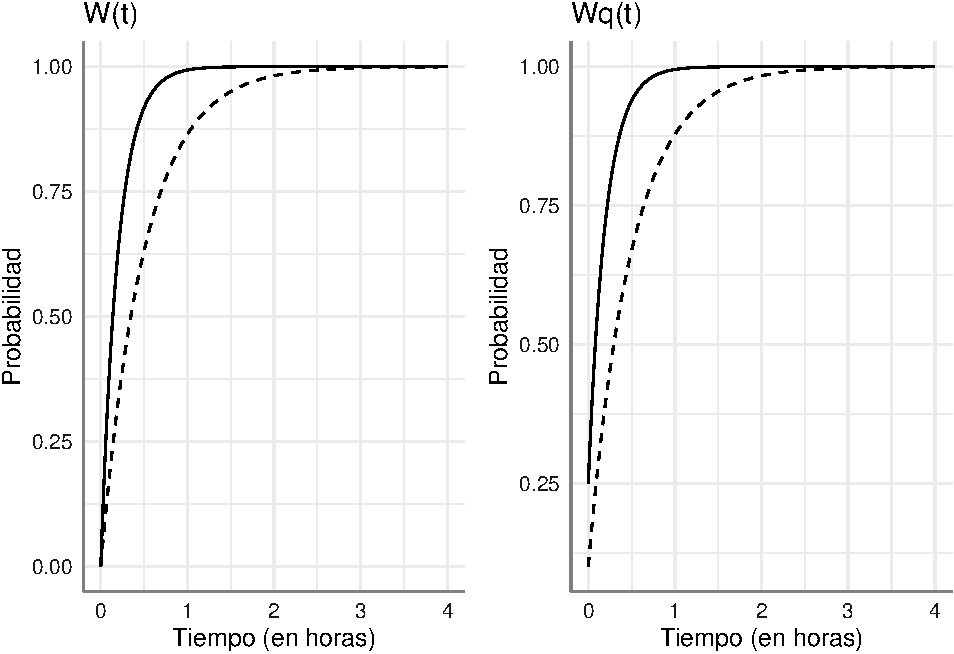
\includegraphics[width=0.95\linewidth]{05-Colas_files/figure-latex/colas-012-1} 

}

\caption{Funciones de distribución de W y Wq para ambos sistemas (sistema 1 = línea continua, sistema 2 = línea discontinua.}\label{fig:colas-012}
\end{figure}

Como se puede ver los tiempos medios de espera de los clientes en el sistema y en la cola para la segunda opción tienen probabildides más bajas a lo largo del tiempo, lo que indica que el sistema está más congestionado porque los tiempos de atención son superiores (valores donde se alcanza la probabilidad 1).

\hypertarget{mm1k}{%
\subsection{M/M/1/K}\label{mm1k}}

Se trata de un modelo como el \(M/M/1\), ya estudiado, pero con límitación \(K\) para el tamaño de la cola. Es decir, la distribución del tiempo entre dos intentos de llegadas al sistema de clientes consecutivos es un PP de tasa \(\lambda\), mietras que la distribución del tiempo de servicio es exponencial de media \(1/\mu\) y sólo hay un servidor. Además el número de clientes que pueden estar en la cola es como mucho \(K\), la población potencial es infinita y la disciplina es FIFO. Obviamente, en este modelo se puede dar el caso de que un cliente que intente entrar en el sistema no lo consiga, por estar la cola llena.

En esta situación tenemos que las tasas de llegadas viene dadas por:

\[
\lambda_n =
\begin{cases}
\lambda & \text{ si } n = 0, 1,...,K\\
0 & \text{ si } n = K+1, K+2,...
\end{cases}
\]
mientras que las tasas de servicio se corresponden con la cola \(M/M/1\)

\[
\mu_n = \mu, \quad n = 1, 2,...
\]
donde a partir de las ecuaciones de equilibrio podemos obtener la relación entre tasas de llegadas y servicio:

\[
c_n =
\begin{cases}
\rho^n & \text{ si } n = 0, 1,...,K, K+1\\
0 & \text{ si } n = K+2, K+3,...
\end{cases}
\]
En este caso, por muy frecuente que sea la llegada de clientes al sistema en relación con la capacidad del servidor para dar servicio, la propia limitación en el tamaño de la cola fuerza a la estacionariedad, pues lo peor que podríamos imaginar es que prácticamente todo el tiempo estuviese el sistema saturado (es decir \(P(N = K + 1) = 1\)). Para analizar el comportamiento de la serie distinguiremos que \(\rho \neq 1\) y \(\rho = 1\).

\textbf{Caso \(\rho \neq 1\)}

De esta forma, la distribución de probabilidad de la variable aleatoria del ``número de clientes en el sistema'' es:

\[
P(N = n) = p_n =
\begin{cases}
\frac{\rho - 1}{\rho^{K+2} - 1} \rho^n & \text{ si } n = 0, 1,..., K+1\\
0  & \text{ si } n = K+2, K+3,...
\end{cases}
\]

El número medio de clientes en el sistema es:

\[L = \frac{\rho}{1 - \rho} - \frac{(K + 2)\rho^{K+2}}{1 - \rho^{K+2}}\]

Dado que las tasas de llegada no son contantes, necesitamos obtener el valor de \(\bar{\lambda}\) para aplicar la fórmula de Little al resto de cantidades de interés. En este caso:

\[\bar{\lambda} = \frac{\lambda(\rho^{K+1} - 1)}{\rho^{K+1} - 1}\]

A partir de esta expresión podemos obtener el tiempo medio de espera de los clientes en la cola como:

\[W = \frac{1}{\mu - \lambda} - \frac{(K+1)\rho^{K+2}}{\lambda(1-\rho^{K+1})}\]

De la relación entre \(W\) y \(W_q\) podemos obtener:

\[W_q = \frac{\lambda}{\mu(\mu - \lambda)} - \frac{(K+1)\rho^{K+2}}{\lambda(1-\rho^{K+1})}\]
Por último:

\[L_q =  \frac{\rho^2}{1 - \rho} - \frac{(K + 1 + \rho)\rho^{K+2}}{1 - \rho^{K+2}}\]

\textbf{Caso \(\rho = 1\)}

En este caso las fórmulas anteriroes se simplifican a:

\[p_n = \frac{1}{K+2}, \text{ para } n = 0, 1,...,K + 1\]
\[L = \frac{K + 1}{2}\]
\[\bar{\lambda} = \frac{\lambda(K + 1)}{K + 2}\]

\[W = \frac{K + 2}{2\lambda}\]
\[W_q = \frac{K}{2\lambda}\]
\[L_q = \frac{K(K + 1)}{2(K+2)}\]

En este modelo (y en otros posteriores) el significado de \(\rho\) como intensidad de tráfico se desvirtúa. Aquí \(\rho\) no puede interpretarse como el cociente entre número medio de llegadas de clientes al sistema por unidad de tiempo y el número medio de clientes a los que el servidor tendría capacidad de dar servicio por unidad de tiempo, sinó más bien como un cociente semejante, pero donde el númerador representa el número medio de intentos de llegada, más que de llegadas efectivas al sistema. De hecho, por este motivo \(\rho\) puede ser mayor o igual que 1, aún siendo el sistema estacionario.
El valor de \(\bar{\lambda}\) sí representa el número medio de entradas efectivas de clientes en el sistema por unidad de tiempo y, así, la verdadera intensidad de tráfico podría medirse a través de:

\[
\bar{\rho} = \frac{\bar{\lambda}}{\mu} =
\begin{cases}
\frac{K+1}{K+2} & \text{ si } \rho = 1 \\
\frac{\rho^{K+2}-\rho}{\rho^{K+2}-1} & \text{ si } \rho \neq 1 
\end{cases}
\]
que efectivamente sí es siempre menor que 1.

::: \{.example name = ``Taller Mecánico''\}

En un taller mecánico llegan vehículos para una puesta a punto antes de pasar la ITV, las llegadas siguen un proceso de Poisson de promedio 18 vehículos/hora. Las dimensiones del taller sólo permiten que haya 4 vehículos, y las ordenanzas municipales no permiten esperar en la vía pública. El taller despacha un promedio de 6 vehículos/hora de acuerdo con una distribución exponencial. Se pide:

\begin{itemize}
\tightlist
\item
  ¿Cuál es la probabilidad de que no haya ningún vehículo en el taller?
\item
  ¿Cuál es el promedio de vehículos en el taller?
\item
  ¿Cuánto tiempo pasa por término medio un vehículo en el taller?
\item
  ¿Cuánto tiempo esperan por término medio los vehículos en la cola?
\item
  ¿Cuál es la longitud media de la cola?
\end{itemize}

:::

Se trata de un sistema \(M/M/1/K\) con \(K = 4\), y utilizaremos la librería \texttt{queueing} para los cálculos numéricos. Si tomamos como unidad de tiempo las horas tendremos que \(\lambda = 18\) y \(\mu = 6\). Geenramos el sistema de cola definido y procedemos con los cálculos solicitados.

\begin{Shaded}
\begin{Highlighting}[]
\CommentTok{\# Deficición del entorno}
\NormalTok{env.MM1K }\OtherTok{\textless{}{-}} \FunctionTok{NewInput.MM1K}\NormalTok{(}\AttributeTok{lambda =} \DecValTok{18}\NormalTok{, }\AttributeTok{mu =} \DecValTok{6}\NormalTok{, }\AttributeTok{k =} \DecValTok{4}\NormalTok{)}
\CommentTok{\# Características del sistema}
\NormalTok{s.MM1K }\OtherTok{\textless{}{-}} \FunctionTok{QueueingModel}\NormalTok{(env.MM1K)}
\end{Highlighting}
\end{Shaded}

Las medidas proporcionadas por la función son las mismas que con el modelo \(M/M/1\). Comenzamos a responder las preguntas:

\begin{itemize}
\tightlist
\item
  Apartado 1. La probabilidad de que no haya ningún vehículo en el taller es \(p_0\):
\end{itemize}

\begin{Shaded}
\begin{Highlighting}[]
\NormalTok{s.MM1K}\SpecialCharTok{$}\NormalTok{Pn[}\DecValTok{1}\NormalTok{]}
\end{Highlighting}
\end{Shaded}

\begin{verbatim}
## [1] 0.008264463
\end{verbatim}

\begin{itemize}
\tightlist
\item
  Apartado 2. Obtenemos el número medio de vehículos en el sistema \(L\):
\end{itemize}

\begin{Shaded}
\begin{Highlighting}[]
\NormalTok{s.MM1K}\SpecialCharTok{$}\NormalTok{L}
\end{Highlighting}
\end{Shaded}

\begin{verbatim}
## [1] 3.520661
\end{verbatim}

\begin{itemize}
\tightlist
\item
  Apartado 3. En este caso estamos interesados en el tiempo medio de estancia en el sistema (\(W\)):
\end{itemize}

\begin{Shaded}
\begin{Highlighting}[]
\NormalTok{s.MM1K}\SpecialCharTok{$}\NormalTok{W}
\end{Highlighting}
\end{Shaded}

\begin{verbatim}
## [1] 0.5916667
\end{verbatim}

\begin{itemize}
\tightlist
\item
  Apartado 4. En este caso estamos interesados en el tiempo medio de estancia en la cola (\(W_q\)):
\end{itemize}

\begin{Shaded}
\begin{Highlighting}[]
\NormalTok{s.MM1K}\SpecialCharTok{$}\NormalTok{Wq}
\end{Highlighting}
\end{Shaded}

\begin{verbatim}
## [1] 0.425
\end{verbatim}

\begin{itemize}
\tightlist
\item
  Apartado 5. En este caso estamos interesados en el número medio de clientes en la cola (\(L_q\)):
\end{itemize}

\begin{Shaded}
\begin{Highlighting}[]
\NormalTok{s.MM1K}\SpecialCharTok{$}\NormalTok{Lq}
\end{Highlighting}
\end{Shaded}

\begin{verbatim}
## [1] 2.528926
\end{verbatim}

\begin{bluebox}
Para el resto de sistemas de colas que vamos a presentar no desarrollaremos de forma completa todas las fórmulas teóricas, y nos centraremos en los resultados numéricos que proporciona la libreria \texttt{queueing} para la resolución de aplicaciones.

\end{bluebox}

\hypertarget{COLASD}{%
\section{Colas con múltiples servidores}\label{COLASD}}

Generalizamos los modelos anteriores a situaciones donde tenemos múltiples servidores.

\hypertarget{mms}{%
\subsection{M/M/s}\label{mms}}

Es una generalización del modelo \(M/M/1\) en el caso en que haya \(s\) servidores. Se trata pues de una cola en la que la distribución del tiempo entre llegadas consecutivas es una \(exp(\lambda)\), la distribución del tiempo de servicio es \(exp(\mu)\) y hay \(s\) servidores. En este caso la población potencial y la capacidad de la cola son infinitas y la disciplina de la cola es FIFO.

Las tasas de llegadas vienen dadas por

\[\lambda_n = \lambda, \text{ para } n = 0, 1,...\]
y las tasas de servicio

\[\mu_n = 
\begin{cases}
n\mu & \text{ si } n = 1, 2,...,s\\
s\mu & \text{ si } n = s+1, s+2,...
\end{cases}
\]

con ratio de ocupación

\[\rho = \frac{\lambda}{\mu s}\]

A partir de las ecuaciones de equilibrio podemos obtener la relación entre tasas de llegadas y servicio:

\[
c_n =
\begin{cases}
\frac{\lambda^n}{n!\mu^n} & \text{ si } n = 0, 1,...,s\\
\frac{\lambda^s}{s!\mu^s}\rho^{n-s} & \text{ si } n = s+1, s+2,...
\end{cases}
\]

La suma de la serie de los \(c_n\) será convergente (el sistema es estacionario) si \(\rho < 1\), es decir,
\(\lambda < s\mu\).

\begin{example}

En una determinada planta de fabricación, la operación final es una operación de pintura. En el centro de pintura siempre hay dos trabajadores que trabajan en paralelo, aunque debido a la configuración física, no pueden ayudarse mutuamente. Las llegdas al centro de pintura se producen según un proceso de Poisson con
con una tasa de llegada media de 100 al día. Cada trabajador tarda una media de 27 minutos en pintar cada artículo. Últimamente, el exceso de trabajo en curso es motivo de preocupación, por lo que la dirección está considerando ampliar el centro de pintura y contratar a un tercer trabajador. (Se supone que el tercer trabajador, tras un periodo de formación, también tardará una media de 27 minutos por pieza). Otra opción sería comprar un robot para realizar la tarea de los trabajadores, ya que se sabe que el tiempo medio que tardará en cada pieza es de 10 minutos.

\begin{itemize}
\tightlist
\item
  Analiza cada uno de los tres sistemas respecto de las medidas de eficiencia e indica que alternativa reduciría el inventario.
\item
  El coste del inventario (incluyendo la pieza que se está trabajando) se estima en 0,50 euros por pieza y hora. El coste por trabajador (salario y gastos generales) se estima en 40.000 euros al año, y el coste de instalación y mantenimiento de un robot se estima en 100.000 euros al año ¿Qué alternativa, si es que hay alguna, es justificable utilizando un criterio de coste esperado a largo plazo?
\end{itemize}

\end{example}

Se proponen tres sistemas de colas con las características siguientes (utilizando como unidad de tiempo las horas):

\begin{itemize}
\tightlist
\item
  Situación 1. Cola \(M/M/2\) con \(\lambda = 100/24\) y \(\mu = 60/27\)
\item
  Situación 2. Cola \(M/M/3\) con \(\lambda = 100/24\) y \(\mu = 60/27\)
\item
  Situación 3. Cola \(M/M/1\) con \(\lambda = 100/24\) y \(\mu = 60/10\)
\end{itemize}

Para determinar que sistema mejoraría el estado del inventario utilizamos varias medidas relativas a cada uno de ellos:

\begin{itemize}
\tightlist
\item
  ratio de ocupación,
\item
  probabilidad de que el sistema este ocupado,
\item
  tiempo medio de las piezas en el sistema.
\end{itemize}

Definimos los tres sistemas y obtenemos las medidas de interés. Para los sistemas \(M/M/s\) utilizaremos la función \texttt{NewInput.MMC}, donde el parámetro \(c\) indica el número de servidores. Generamos los tres sistemas:

\begin{Shaded}
\begin{Highlighting}[]
\CommentTok{\# Parámetros de los sistemas}
\NormalTok{lambda }\OtherTok{\textless{}{-}} \DecValTok{100}\SpecialCharTok{/}\DecValTok{24}
\NormalTok{muk }\OtherTok{\textless{}{-}} \DecValTok{60}\SpecialCharTok{/}\DecValTok{27}
\NormalTok{mu1 }\OtherTok{\textless{}{-}} \DecValTok{60}\SpecialCharTok{/}\DecValTok{10}

\CommentTok{\# M/M/2}
\NormalTok{env.MM2 }\OtherTok{\textless{}{-}} \FunctionTok{NewInput.MMC}\NormalTok{(}\AttributeTok{lambda =}\NormalTok{ lambda, }\AttributeTok{mu =}\NormalTok{ muk, }\AttributeTok{c =} \DecValTok{2}\NormalTok{, }\AttributeTok{n =} \DecValTok{2}\NormalTok{)}
\NormalTok{s.MM2 }\OtherTok{\textless{}{-}} \FunctionTok{QueueingModel}\NormalTok{(env.MM2)}
\CommentTok{\# M/M/3}
\NormalTok{env.MM3 }\OtherTok{\textless{}{-}} \FunctionTok{NewInput.MMC}\NormalTok{(}\AttributeTok{lambda =}\NormalTok{ lambda, }\AttributeTok{mu =}\NormalTok{ muk, }\AttributeTok{c =} \DecValTok{3}\NormalTok{, }\AttributeTok{n =} \DecValTok{2}\NormalTok{)}
\NormalTok{s.MM3 }\OtherTok{\textless{}{-}} \FunctionTok{QueueingModel}\NormalTok{(env.MM3)}
\CommentTok{\# M/M/1}
\NormalTok{env.MM1 }\OtherTok{\textless{}{-}} \FunctionTok{NewInput.MM1}\NormalTok{(}\AttributeTok{lambda =}\NormalTok{ lambda, }\AttributeTok{mu =}\NormalTok{ mu1, }\AttributeTok{n =} \DecValTok{2}\NormalTok{)}
\NormalTok{s.MM1 }\OtherTok{\textless{}{-}} \FunctionTok{QueueingModel}\NormalTok{(env.MM1)}
\end{Highlighting}
\end{Shaded}

Obtenemos y comparamos las diferentes medidas consideradas

\begin{Shaded}
\begin{Highlighting}[]
\CommentTok{\# ratio de ocupación}
\FunctionTok{c}\NormalTok{(s.MM2}\SpecialCharTok{$}\NormalTok{RO, s.MM3}\SpecialCharTok{$}\NormalTok{RO, s.MM1}\SpecialCharTok{$}\NormalTok{RO)}
\end{Highlighting}
\end{Shaded}

\begin{verbatim}
## [1] 0.9375000 0.6250000 0.6944444
\end{verbatim}

\begin{Shaded}
\begin{Highlighting}[]
\CommentTok{\# Probabildid de que el sistema este ocupado}
\FunctionTok{c}\NormalTok{(}\DecValTok{1}\SpecialCharTok{{-}}\NormalTok{s.MM2}\SpecialCharTok{$}\NormalTok{Pn[}\DecValTok{1}\NormalTok{], }\DecValTok{1}\SpecialCharTok{{-}}\NormalTok{s.MM3}\SpecialCharTok{$}\NormalTok{Pn[}\DecValTok{1}\NormalTok{], }\DecValTok{1}\SpecialCharTok{{-}}\NormalTok{s.MM1}\SpecialCharTok{$}\NormalTok{Pn[}\DecValTok{1}\NormalTok{])}
\end{Highlighting}
\end{Shaded}

\begin{verbatim}
## [1] 0.9677419 0.8677686 0.6944444
\end{verbatim}

\begin{Shaded}
\begin{Highlighting}[]
\CommentTok{\# Tiempo medio en el sistema}
\FunctionTok{c}\NormalTok{(s.MM2}\SpecialCharTok{$}\NormalTok{W, s.MM3}\SpecialCharTok{$}\NormalTok{W, s.MM1}\SpecialCharTok{$}\NormalTok{W)}
\end{Highlighting}
\end{Shaded}

\begin{verbatim}
## [1] 3.7161290 0.6049587 0.5454545
\end{verbatim}

Desde el punto de vista de ratio de ocupación el mejor sistema sería el de tres trabajores, pero si utilizamos los otros dos criterios el mejor sistema sería el que utiliza el robot.

Hacemos ahora la evaluación de costes por hora teniendo en cuenta que cada año tiene 8760 horas (365*24). Para obtener los costes asociados debemos estimar el número de piezas en el sistema por hora para evaluar el coste total de inventario, ay añadir el coste de la mano de obra. En esta situación tenemos:

\begin{Shaded}
\begin{Highlighting}[]
\CommentTok{\# Coste M/M/2}
\NormalTok{s.MM2}\SpecialCharTok{$}\NormalTok{L}\SpecialCharTok{*}\FloatTok{0.50} \SpecialCharTok{+} \DecValTok{2}\SpecialCharTok{*}\NormalTok{(}\DecValTok{40000}\SpecialCharTok{/}\DecValTok{8760}\NormalTok{)}
\end{Highlighting}
\end{Shaded}

\begin{verbatim}
## [1] 16.87436
\end{verbatim}

\begin{Shaded}
\begin{Highlighting}[]
\CommentTok{\# Coste M/M/3}
\NormalTok{s.MM3}\SpecialCharTok{$}\NormalTok{L}\SpecialCharTok{*}\FloatTok{0.50} \SpecialCharTok{+} \DecValTok{3}\SpecialCharTok{*}\NormalTok{(}\DecValTok{40000}\SpecialCharTok{/}\DecValTok{8760}\NormalTok{)}
\end{Highlighting}
\end{Shaded}

\begin{verbatim}
## [1] 14.95896
\end{verbatim}

\begin{Shaded}
\begin{Highlighting}[]
\CommentTok{\# Coste M/M/1}
\NormalTok{s.MM3}\SpecialCharTok{$}\NormalTok{L}\SpecialCharTok{*}\FloatTok{0.50} \SpecialCharTok{+}\NormalTok{ (}\DecValTok{100000}\SpecialCharTok{/}\DecValTok{8760}\NormalTok{)}
\end{Highlighting}
\end{Shaded}

\begin{verbatim}
## [1] 12.67586
\end{verbatim}

Atendiendo a los costes, el modelo que utiliza el robot resulta en un menor coste por hora por lo que resulta el más beneficioso.

\hypertarget{mmsk}{%
\subsection{M/M/s/K}\label{mmsk}}

Es una generalización del modelo \(M/M/1/K\) en el caso en que haya \(s\) servidores. Las tasas de llegada son casi idénticas a las del modelo \(M/M/1\), mientras que las de servicio son exáctamente iguales a las de un \(M/M/s\):

\[\lambda_n = 
\begin{cases}
\lambda \text{ para } n = 0, 1,..., K+s-1\\
0 \text{ para } n = K+s, K+s+1,...
\end{cases}
\]

\[\mu_n = 
\begin{cases}
n\mu & \text{ si } n = 1, 2,...,s\\
s\mu & \text{ si } n = s+1, s+2,...
\end{cases}
\]

con ratio efectivo de ocupación

\[\bar{\rho} = \frac{\bar{\lambda}}{\mu s}\]

Este sistema siempre es estacionario. A continuación, se presenta un ejemplo de este sistema donde se muestra la función que debemos usar para analiar este tipo de cola.

\begin{example}

Por razones técnicas, una centralita con dos operadoras sólo permite mantener tres llamadas en espera (de tal forma que cualquier llamada producida cuando ya hay dos siendo atendidas por las operadoras y otras tres en espera, recibe el tono de ``línea ocupada''). Las llamadas llegan según un proceso de Poisson, a razón de 6 por minuto, siendo l5 segundos la media del tiempo que tarda cada operadora en direccionar una llamada y dicho tiempo de distribución exponencial. Calcular:

\begin{itemize}
\tightlist
\item
  El porcentaje de tiempo en que cada operadora está ocupada y el número medio de servidores ocupados.
\item
  El número medio de llamadas en espera.
\item
  La probabilidad de que una llamada obtenga la señal de ``línea ocupada''.
\item
  Calcular las tres cantidades anteriores bajo el supuesto de que se amplie a 5 las llamadas en espera.
\end{itemize}

\end{example}

Para el análisis de este sistema utilizamos la función \texttt{NewInput.MMCK} donde además de las tasas, debemos indicar el número de servidores, y la capacidad del sistema. Tomaremos como unidad de tiempo los minutos de forma que \(\lambda = 6\) y \(\mu = 60/15 = 4\). La capacidad del sistema es \(K = 5\) que se corresponde con dos llamadas atendidas y tres en espera. Se trata pues de un sistema \(M/M/2/5\).

\begin{Shaded}
\begin{Highlighting}[]
\CommentTok{\# M/M/2/5}
\NormalTok{env.MM25 }\OtherTok{\textless{}{-}} \FunctionTok{NewInput.MMCK}\NormalTok{(}\AttributeTok{lambda =} \DecValTok{6}\NormalTok{, }\AttributeTok{mu =} \DecValTok{4}\NormalTok{, }\AttributeTok{c =} \DecValTok{2}\NormalTok{, }\AttributeTok{k =} \DecValTok{5}\NormalTok{)}
\NormalTok{s.MM25 }\OtherTok{\textless{}{-}} \FunctionTok{QueueingModel}\NormalTok{(env.MM25)}
\end{Highlighting}
\end{Shaded}

\begin{verbatim}
## Warning in formals(fun): argument is not a function

## Warning in formals(fun): argument is not a function

## Warning in formals(fun): argument is not a function

## Warning in formals(fun): argument is not a function

## Warning in formals(fun): argument is not a function

## Warning in formals(fun): argument is not a function

## Warning in formals(fun): argument is not a function
\end{verbatim}

Veamos como responder a cada una de las cuestiones planteadas utilizando los resultados del sistema diseñado. para responder al primer apartado debemos obtener el ratio efectivo de ocupación, asi como la diferencia entre el número medio de clientes en el sistema y el número medio de clientes en la cola para determinar el número medio de servidores ocupados.

\begin{Shaded}
\begin{Highlighting}[]
\CommentTok{\# Porcentaje de tiempo servidor ocupado}
\FunctionTok{round}\NormalTok{(}\DecValTok{100}\SpecialCharTok{*}\NormalTok{s.MM25}\SpecialCharTok{$}\NormalTok{RO, }\DecValTok{2}\NormalTok{)}
\end{Highlighting}
\end{Shaded}

\begin{verbatim}
## [1] 68.62
\end{verbatim}

\begin{Shaded}
\begin{Highlighting}[]
\CommentTok{\# Número medio de servidores ocupados}
\NormalTok{s.MM25}\SpecialCharTok{$}\NormalTok{L }\SpecialCharTok{{-}}\NormalTok{ s.MM25}\SpecialCharTok{$}\NormalTok{Lq}
\end{Highlighting}
\end{Shaded}

\begin{verbatim}
## [1] 1.372329
\end{verbatim}

La ocupación de cada operadora es del 68.6\% y el número medio de operadores ocupados es del 1.4. Con respecto al número medio de llamadas en espera tenemos:

\begin{Shaded}
\begin{Highlighting}[]
\CommentTok{\# Número medio de llamadas en espera}
\NormalTok{s.MM25}\SpecialCharTok{$}\NormalTok{Lq}
\end{Highlighting}
\end{Shaded}

\begin{verbatim}
## [1] 0.6336252
\end{verbatim}

En cuanto a la probabilidad solicitada debemos calcular \(P(N_q = 3) = P(N = 5)\) que se obtiene como:

\begin{Shaded}
\begin{Highlighting}[]
\CommentTok{\# Probabilidad de linea ocupada}
\NormalTok{s.MM25}\SpecialCharTok{$}\NormalTok{Pn[}\DecValTok{6}\NormalTok{]}
\end{Highlighting}
\end{Shaded}

\begin{verbatim}
## [1] 0.08511384
\end{verbatim}

Tan solo en un 8.5\% de las ocasiones salta el mensaje de línea ocupada, es decir, el sistema esta ocupado al 100\%.

Evaluamos ahora el incremento del tamaño de sistema aumentado las llamadas en espera.

\begin{Shaded}
\begin{Highlighting}[]
\CommentTok{\# M/M/2/7}
\NormalTok{env.MM27 }\OtherTok{\textless{}{-}} \FunctionTok{NewInput.MMCK}\NormalTok{(}\AttributeTok{lambda =} \DecValTok{6}\NormalTok{, }\AttributeTok{mu =} \DecValTok{4}\NormalTok{, }\AttributeTok{c =} \DecValTok{2}\NormalTok{, }\AttributeTok{k =} \DecValTok{7}\NormalTok{)}
\NormalTok{s.MM27 }\OtherTok{\textless{}{-}} \FunctionTok{QueueingModel}\NormalTok{(env.MM27)}
\end{Highlighting}
\end{Shaded}

\begin{verbatim}
## Warning in formals(fun): argument is not a function

## Warning in formals(fun): argument is not a function

## Warning in formals(fun): argument is not a function

## Warning in formals(fun): argument is not a function

## Warning in formals(fun): argument is not a function

## Warning in formals(fun): argument is not a function

## Warning in formals(fun): argument is not a function
\end{verbatim}

\begin{Shaded}
\begin{Highlighting}[]
\CommentTok{\# Porcentaje de tiempo servidor ocupado}
\FunctionTok{round}\NormalTok{(}\DecValTok{100}\SpecialCharTok{*}\NormalTok{s.MM27}\SpecialCharTok{$}\NormalTok{RO, }\DecValTok{2}\NormalTok{)}
\end{Highlighting}
\end{Shaded}

\begin{verbatim}
## [1] 71.77
\end{verbatim}

\begin{Shaded}
\begin{Highlighting}[]
\CommentTok{\# Número medio de servidores ocupados}
\NormalTok{s.MM27}\SpecialCharTok{$}\NormalTok{L }\SpecialCharTok{{-}}\NormalTok{ s.MM27}\SpecialCharTok{$}\NormalTok{Lq}
\end{Highlighting}
\end{Shaded}

\begin{verbatim}
## [1] 1.435402
\end{verbatim}

\begin{Shaded}
\begin{Highlighting}[]
\CommentTok{\# Número medio de llamadas en espera}
\NormalTok{s.MM27}\SpecialCharTok{$}\NormalTok{Lq}
\end{Highlighting}
\end{Shaded}

\begin{verbatim}
## [1] 1.014966
\end{verbatim}

\begin{Shaded}
\begin{Highlighting}[]
\CommentTok{\# Probabilidad de linea ocupada}
\NormalTok{s.MM27}\SpecialCharTok{$}\NormalTok{Pn[}\DecValTok{8}\NormalTok{]}
\end{Highlighting}
\end{Shaded}

\begin{verbatim}
## [1] 0.04306559
\end{verbatim}

\hypertarget{COLASE}{%
\section{Redes de colas en serie}\label{COLASE}}

Una red de colas en serie es una colección de \(K\) colas que se suceden unas a otras de tal manera que sólo es posible la entrada de clientes dede fuera del sistema a la primera de ellas, produciéndose la salida de ellas tras el servicio de la última cola. En esta situación podemos definir las medidas de eficiencia del sistema completo de colas en función de las medidas de efiecencia de cada una de las colas que conforman el sistema, teniendo en cuenta que tan sólo hay una tasa de llegada que corresponde con la cola inicial de la red.

Imaginemos \(i=1,2,...,k\) colas en red del tipo \(M/M/s_i\) independientes con tasa de entrada \(\lambda\) y tasa de servicio \(\mu_i\), y con medidas de eficiencia \(L_i, W_i, L_{q_i}, W_{q_i}\). Dadoq ue en este caso el flujo de un cliente a través de la red es secuencial será cierto que los tiempos medios de un cliente en la red son la suma de los correspondientes a cada subsistema. Si denotamos por \(L_{red}, W_{red}, L_{q_{red}}, W_{q_{red}}\) las medidas de eficencia del sistema, aplicando este razonamiento tenemos que:

\[L_{red} = \sum_{i = 1}^k L_i\]

\[W_{red} = \sum_{i = 1}^k W_i\]

\[W_{q_{red}} = W_{red} - \left(\sum_{i = 1}^k \frac{1}{\mu_i}\right)\]

\[L_{q_{red}} = \lambda W_{q_{red}}\]

de esta forma basta con analizar cada una de las clas que conforman la red para estudiar el comportamiento global del sistema.

\begin{example}

Una empresa de ITV en una localidad dispone de una superficie que consta de tres partes: Una caseta donde los clientes entregan la documentación del vehículo y realizan el pago de tasas, sin restricciones paa atender ningún vehículo. Una nave formada por dos circuitos (revisión y oficina de personal técnico) atendidos por dos técnicos cada uno de ellos. Los vehículos que llegan a la nave son atendidos con una tasa de servicio medio de 45 clientes/hora para la revisión y 2 minutos/cliente en la oficina de personal técnico. Los coches acuden a la empresa a una media de 57 clientes/hora, ya que un mayor número de vehículos colapsaría el trabajo de la caseta, cuyo empleado atiende a un ritmo medio de 1 cliente/minuto. Las llegadas siguen un Proceso de Poisson y los tiempos de servicio se distribuyen según una variable exponencial. Se pide:

\begin{itemize}
\tightlist
\item
  Factor de utilziación o intensidad de tráfico en cada nodo de la red.
\item
  Probabildiades de que no haya ningún cliente en cada uno de los nodos de la red.
\item
  Longitud media de la cola de vehículos que habiendo pagado las tasas se encuentran esperando a la entrada de la nave.
\item
  Tiempo medio que un cliente pasa en la revisión.
\item
  Tiempo medio que un cliente pasa en la oficina de personal técnico.
\item
  Tiempo medio que un cliente se encuentra en la ITV.
\item
  Para agilizar el proceso la empresa estudia la posibilidad de ampliar el número de servidores en la caseta o en la oficina. Suponiendo que el coste de ampliación en uno u otro lugar fuera equivalente, ¿qué criterio sería más acertado para que el tiempo de servicio del sistema fuera menor?
\end{itemize}

\end{example}

El sistema se puede describir com una red de colas en serie con nodos: caseta (\(M/M/1\)), equipamiento (\(M/M/2\)) y personal técnico (\(M/M/2\)), con tasas de llegadas y servicio (expresadas en minutos) dadas por:

\[\lambda_1 = \lambda_2 = \lambda_3 = 57/60 = 0.95\]

\[\mu_1 = 1; \mu_2 = 45/60 = 0.75; \mu_3 = 1/2 = 0.5\]

Planteamos los tres sistemas de colas y obtenemos las correspondientes medidas de eficiencia:

\begin{Shaded}
\begin{Highlighting}[]
\CommentTok{\# M/M/1}
\NormalTok{nodo1 }\OtherTok{\textless{}{-}} \FunctionTok{QueueingModel}\NormalTok{(}\FunctionTok{NewInput.MM1}\NormalTok{(}\AttributeTok{lambda =} \FloatTok{0.95}\NormalTok{, }\AttributeTok{mu =} \DecValTok{1}\NormalTok{, }\AttributeTok{n =} \DecValTok{15}\NormalTok{))}
\CommentTok{\# M/M/2}
\NormalTok{nodo2 }\OtherTok{\textless{}{-}} \FunctionTok{QueueingModel}\NormalTok{(}\FunctionTok{NewInput.MMC}\NormalTok{(}\AttributeTok{lambda =} \FloatTok{0.95}\NormalTok{, }\AttributeTok{mu =} \FloatTok{0.75}\NormalTok{, }\AttributeTok{c =} \DecValTok{2}\NormalTok{, }\AttributeTok{n =} \DecValTok{15}\NormalTok{))}
\CommentTok{\# M/M/2}
\NormalTok{nodo3 }\OtherTok{\textless{}{-}} \FunctionTok{QueueingModel}\NormalTok{(}\FunctionTok{NewInput.MMC}\NormalTok{(}\AttributeTok{lambda =} \FloatTok{0.95}\NormalTok{, }\AttributeTok{mu =} \FloatTok{0.5}\NormalTok{, }\AttributeTok{c=} \DecValTok{2}\NormalTok{, }\AttributeTok{n =} \DecValTok{15}\NormalTok{))}
\CommentTok{\# Medidas de eficiencia de cada nodo}
\NormalTok{ef.nodo1 }\OtherTok{\textless{}{-}} \FunctionTok{c}\NormalTok{(nodo1}\SpecialCharTok{$}\NormalTok{RO, nodo1}\SpecialCharTok{$}\NormalTok{L, nodo1}\SpecialCharTok{$}\NormalTok{Lq, nodo1}\SpecialCharTok{$}\NormalTok{W, nodo1}\SpecialCharTok{$}\NormalTok{Wq, nodo1}\SpecialCharTok{$}\NormalTok{Pn[}\DecValTok{1}\NormalTok{]) }
\NormalTok{ef.nodo2 }\OtherTok{\textless{}{-}} \FunctionTok{c}\NormalTok{(nodo2}\SpecialCharTok{$}\NormalTok{RO, nodo2}\SpecialCharTok{$}\NormalTok{L, nodo2}\SpecialCharTok{$}\NormalTok{Lq, nodo2}\SpecialCharTok{$}\NormalTok{W, nodo2}\SpecialCharTok{$}\NormalTok{Wq, nodo2}\SpecialCharTok{$}\NormalTok{Pn[}\DecValTok{1}\NormalTok{]) }
\NormalTok{ef.nodo3 }\OtherTok{\textless{}{-}} \FunctionTok{c}\NormalTok{(nodo3}\SpecialCharTok{$}\NormalTok{RO, nodo3}\SpecialCharTok{$}\NormalTok{L, nodo3}\SpecialCharTok{$}\NormalTok{Lq, nodo3}\SpecialCharTok{$}\NormalTok{W, nodo3}\SpecialCharTok{$}\NormalTok{Wq, nodo3}\SpecialCharTok{$}\NormalTok{Pn[}\DecValTok{1}\NormalTok{])}
\NormalTok{eficiencia }\OtherTok{\textless{}{-}} \FunctionTok{data.frame}\NormalTok{(}\FunctionTok{rbind}\NormalTok{(ef.nodo1, ef.nodo2, ef.nodo3))}
\FunctionTok{names}\NormalTok{(eficiencia) }\OtherTok{\textless{}{-}}\FunctionTok{c}\NormalTok{(}\StringTok{"Ro"}\NormalTok{, }\StringTok{"L"}\NormalTok{, }\StringTok{"Lq"}\NormalTok{, }\StringTok{"W"}\NormalTok{, }\StringTok{"Wq"}\NormalTok{,}\StringTok{"P\_0"}\NormalTok{) }
\NormalTok{eficiencia}
\end{Highlighting}
\end{Shaded}

\begin{verbatim}
##                 Ro         L         Lq         W         Wq        P_0
## ef.nodo1 0.9500000 19.000000 18.0500000 20.000000 19.0000000 0.05000000
## ef.nodo2 0.6333333  2.115028  0.8483612  2.226345  0.8930118 0.22448980
## ef.nodo3 0.9500000 19.487179 17.5871795 20.512821 18.5128205 0.02564103
\end{verbatim}

\hypertarget{COLASF}{%
\section{Funciones simmer}\label{COLASF}}

En este apartado se presentan los algoritmos de simulación de simmer para los sistemas de colas estudiados.

\hypertarget{mm1-1}{%
\subsection{\texorpdfstring{\(M/M/1\)}{M/M/1}}\label{mm1-1}}

\begin{Shaded}
\begin{Highlighting}[]
\CommentTok{\# Sistema}
\DocumentationTok{\#\#\#\#\#\#\#\#\#\#\#\#\#\#\#\#\#\#\#\#\#\#\#\#\#\#\#\#\#\#\#\#\#\#\#\#\#\#\#\#\#\#\#\#\#\#\#\#\#}
\NormalTok{cola.MM1 }\OtherTok{\textless{}{-}} \ControlFlowTok{function}\NormalTok{(t, lambda, mu)}
\NormalTok{\{}
  \CommentTok{\# lambda: tasa de llegadas}
  \CommentTok{\# mu: tasa de servicio}

  \CommentTok{\# Funciones de tiempos}
\NormalTok{  tarrival }\OtherTok{\textless{}{-}} \ControlFlowTok{function}\NormalTok{() }\FunctionTok{rexp}\NormalTok{(}\DecValTok{1}\NormalTok{, lambda)}
\NormalTok{  tserver }\OtherTok{\textless{}{-}} \ControlFlowTok{function}\NormalTok{() }\FunctionTok{rexp}\NormalTok{(}\DecValTok{1}\NormalTok{, mu)}
  
  \CommentTok{\# Trayectoria de servicio}
\NormalTok{  servicio }\OtherTok{\textless{}{-}} \FunctionTok{trajectory}\NormalTok{() }\SpecialCharTok{\%\textgreater{}\%}
    \FunctionTok{visit}\NormalTok{(}\StringTok{"server"}\NormalTok{, tserver)               }

  \CommentTok{\# Entorno del sistema }
  \DocumentationTok{\#\#\#\#\#\#\#\#\#\#\#\#\#\#\#\#\#\#\#\#\#\#\#\#\#\#\#\#\#\#\#\#\#\#\#\#\#\#\#\#\#\#\#\#\#\#\#\#\#}
  \FunctionTok{simmer}\NormalTok{() }\SpecialCharTok{\%\textgreater{}\%}
    \FunctionTok{add\_resource}\NormalTok{(}\StringTok{"server"}\NormalTok{, }\AttributeTok{capacity =} \DecValTok{1}\NormalTok{, }\AttributeTok{queue\_size =} \ConstantTok{Inf}\NormalTok{) }\SpecialCharTok{\%\textgreater{}\%}           
    \FunctionTok{add\_generator}\NormalTok{(}\StringTok{"arrival"}\NormalTok{, servicio, tarrival) }\SpecialCharTok{\%\textgreater{}\%} 
    \FunctionTok{run}\NormalTok{(}\AttributeTok{until =}\NormalTok{ t)     }
\NormalTok{\}}
\end{Highlighting}
\end{Shaded}

\hypertarget{mm1k-1}{%
\subsection{\texorpdfstring{\(M/M/1/K\)}{M/M/1/K}}\label{mm1k-1}}

\begin{Shaded}
\begin{Highlighting}[]
\CommentTok{\# Sistema}
\DocumentationTok{\#\#\#\#\#\#\#\#\#\#\#\#\#\#\#\#\#\#\#\#\#\#\#\#\#\#\#\#\#\#\#\#\#\#\#\#\#\#\#\#\#\#\#\#\#\#\#\#\#}
\NormalTok{cola.MM1K }\OtherTok{\textless{}{-}} \ControlFlowTok{function}\NormalTok{(t, lambda, mu, K)}
\NormalTok{\{}
  \CommentTok{\# lambda: tasa de llegadas}
  \CommentTok{\# mu: tasa de servicio}
  \CommentTok{\# K: capacidad del sistema}

  \CommentTok{\# Funciones de tiempos}
\NormalTok{  tarrival }\OtherTok{\textless{}{-}} \ControlFlowTok{function}\NormalTok{() }\FunctionTok{rexp}\NormalTok{(}\DecValTok{1}\NormalTok{, lambda)}
\NormalTok{  tserver }\OtherTok{\textless{}{-}} \ControlFlowTok{function}\NormalTok{() }\FunctionTok{rexp}\NormalTok{(}\DecValTok{1}\NormalTok{, mu)}
  
  \CommentTok{\# Tamaño de la cola}
\NormalTok{  qsize }\OtherTok{\textless{}{-}}\NormalTok{ K }\SpecialCharTok{{-}} \DecValTok{1}
  
  \CommentTok{\# Trayectoria de servicio}
\NormalTok{  servicio }\OtherTok{\textless{}{-}} \FunctionTok{trajectory}\NormalTok{() }\SpecialCharTok{\%\textgreater{}\%}
    \FunctionTok{visit}\NormalTok{(}\StringTok{"server"}\NormalTok{, tserver)               }

  \CommentTok{\# Entorno del sistema }
  \DocumentationTok{\#\#\#\#\#\#\#\#\#\#\#\#\#\#\#\#\#\#\#\#\#\#\#\#\#\#\#\#\#\#\#\#\#\#\#\#\#\#\#\#\#\#\#\#\#\#\#\#\#}
  \FunctionTok{simmer}\NormalTok{() }\SpecialCharTok{\%\textgreater{}\%}
    \FunctionTok{add\_resource}\NormalTok{(}\StringTok{"server"}\NormalTok{, }\AttributeTok{capacity =} \DecValTok{1}\NormalTok{, }\AttributeTok{queue\_size =}\NormalTok{ qsize) }\SpecialCharTok{\%\textgreater{}\%}           
    \FunctionTok{add\_generator}\NormalTok{(}\StringTok{"arrival"}\NormalTok{, servicio, tarrival) }\SpecialCharTok{\%\textgreater{}\%} 
    \FunctionTok{run}\NormalTok{(}\AttributeTok{until =}\NormalTok{ t)     }
\NormalTok{\}}
\end{Highlighting}
\end{Shaded}

\hypertarget{mms-1}{%
\subsection{\texorpdfstring{\(M/M/s\)}{M/M/s}}\label{mms-1}}

\begin{Shaded}
\begin{Highlighting}[]
\CommentTok{\# Sistema}
\DocumentationTok{\#\#\#\#\#\#\#\#\#\#\#\#\#\#\#\#\#\#\#\#\#\#\#\#\#\#\#\#\#\#\#\#\#\#\#\#\#\#\#\#\#\#\#\#\#\#\#\#\#}
\NormalTok{cola.MMs }\OtherTok{\textless{}{-}} \ControlFlowTok{function}\NormalTok{(t, lambda, mu, s)}
\NormalTok{\{}
  \CommentTok{\# lambda: tasa de llegadas}
  \CommentTok{\# mu: tasa de servicio}
  \CommentTok{\# s: servidores idénticos disponibles}

  \CommentTok{\# Funciones de tiempos}
\NormalTok{  tarrival }\OtherTok{\textless{}{-}} \ControlFlowTok{function}\NormalTok{() }\FunctionTok{rexp}\NormalTok{(}\DecValTok{1}\NormalTok{, lambda)}
\NormalTok{  tserver }\OtherTok{\textless{}{-}} \ControlFlowTok{function}\NormalTok{() }\FunctionTok{rexp}\NormalTok{(}\DecValTok{1}\NormalTok{, mu)}
  
  \CommentTok{\# Trayectoria de servicio}
\NormalTok{  servicio }\OtherTok{\textless{}{-}} \FunctionTok{trajectory}\NormalTok{() }\SpecialCharTok{\%\textgreater{}\%}
    \FunctionTok{visit}\NormalTok{(}\StringTok{"server"}\NormalTok{, tserver)               }

  \CommentTok{\# Entorno del sistema }
  \DocumentationTok{\#\#\#\#\#\#\#\#\#\#\#\#\#\#\#\#\#\#\#\#\#\#\#\#\#\#\#\#\#\#\#\#\#\#\#\#\#\#\#\#\#\#\#\#\#\#\#\#\#}
  \FunctionTok{simmer}\NormalTok{() }\SpecialCharTok{\%\textgreater{}\%}
    \FunctionTok{add\_resource}\NormalTok{(}\StringTok{"server"}\NormalTok{, }\AttributeTok{capacity =}\NormalTok{ s, }\AttributeTok{queue\_size =} \ConstantTok{Inf}\NormalTok{) }\SpecialCharTok{\%\textgreater{}\%}           
    \FunctionTok{add\_generator}\NormalTok{(}\StringTok{"arrival"}\NormalTok{, servicio, tarrival) }\SpecialCharTok{\%\textgreater{}\%} 
    \FunctionTok{run}\NormalTok{(}\AttributeTok{until =}\NormalTok{ t)     }
\NormalTok{\}}
\end{Highlighting}
\end{Shaded}

\hypertarget{mmsk-1}{%
\subsection{\texorpdfstring{\(M/M/s/K\)}{M/M/s/K}}\label{mmsk-1}}

\begin{Shaded}
\begin{Highlighting}[]
\CommentTok{\# Sistema}
\DocumentationTok{\#\#\#\#\#\#\#\#\#\#\#\#\#\#\#\#\#\#\#\#\#\#\#\#\#\#\#\#\#\#\#\#\#\#\#\#\#\#\#\#\#\#\#\#\#\#\#\#\#}
\NormalTok{cola.MMsK }\OtherTok{\textless{}{-}} \ControlFlowTok{function}\NormalTok{(t, lambda, mu, s, K)}
\NormalTok{\{}
  \CommentTok{\# lambda: tasa de llegadas}
  \CommentTok{\# mu: tasa de servicio}
  \CommentTok{\# s: servidores}
  \CommentTok{\# K: capacidad del sistema}

  \CommentTok{\# Funciones de tiempos}
\NormalTok{  tarrival }\OtherTok{\textless{}{-}} \ControlFlowTok{function}\NormalTok{() }\FunctionTok{rexp}\NormalTok{(}\DecValTok{1}\NormalTok{, lambda)}
\NormalTok{  tserver }\OtherTok{\textless{}{-}} \ControlFlowTok{function}\NormalTok{() }\FunctionTok{rexp}\NormalTok{(}\DecValTok{1}\NormalTok{, mu)}
  
  \CommentTok{\# Tamaño de la cola}
\NormalTok{  qsize }\OtherTok{\textless{}{-}}\NormalTok{ K }\SpecialCharTok{{-}}\NormalTok{ s}
  
  \CommentTok{\# Trayectoria de servicio}
\NormalTok{  servicio }\OtherTok{\textless{}{-}} \FunctionTok{trajectory}\NormalTok{() }\SpecialCharTok{\%\textgreater{}\%}
    \FunctionTok{visit}\NormalTok{(}\StringTok{"server"}\NormalTok{, tserver)               }

  \CommentTok{\# Entorno del sistema }
  \DocumentationTok{\#\#\#\#\#\#\#\#\#\#\#\#\#\#\#\#\#\#\#\#\#\#\#\#\#\#\#\#\#\#\#\#\#\#\#\#\#\#\#\#\#\#\#\#\#\#\#\#\#}
  \FunctionTok{simmer}\NormalTok{() }\SpecialCharTok{\%\textgreater{}\%}
    \FunctionTok{add\_resource}\NormalTok{(}\StringTok{"server"}\NormalTok{, }\AttributeTok{capacity =}\NormalTok{ s, }\AttributeTok{queue\_size =}\NormalTok{ qsize) }\SpecialCharTok{\%\textgreater{}\%}           
    \FunctionTok{add\_generator}\NormalTok{(}\StringTok{"arrival"}\NormalTok{, servicio, tarrival) }\SpecialCharTok{\%\textgreater{}\%} 
    \FunctionTok{run}\NormalTok{(}\AttributeTok{until =}\NormalTok{ t)     }
\NormalTok{\}}
\end{Highlighting}
\end{Shaded}

\hypertarget{COLASG}{%
\section{Ejercicios}\label{COLASG}}

Los ejercicios que se presentan a continuación se estruturan en dos niveles de dificultad. El primer nivel son ejercicios más básicos (codificados con una B que provienen de los ejemplso vistos en la unidad), mientras que el segundo bloque necesitan una mayor cantidad de trabajo (codificados con una A). Cuando consideres necesario puedes plantear una solución mediante simulación para contestar a las preguntas de interés.

\textbf{Ejercicio B-1.} Para el ejemplo del sistema de la estación de trabajo descrito para el sistema \(M/M/1\) vamos a contestar a las diferentes cuestiones que allí se planteaban pero considerando que la estación de trabajo dispone de tres servidores idénticos. Hallar también el número medio total de procesos en la estación.

\textbf{Ejercicio A-1.} Los coches llegan a un peaje 24 horas al día según un proceso de Poisson con
una tasa media de 15 por hora. Estamos interesados en:

\begin{itemize}
\tightlist
\item
  ¿Cuál es el número esperado de coches que llegarán a la cabina entre la 1:00 p.m. y 1:30 p.m.?
\item
  ¿Cuál es el tiempo esperado entre dos coches que llegan consecutivamente?
\item
  Son las 13:12 y acaba de llegar un coche. ¿Cuál es el número esperado de coches que llegarán entre este momento y la 1:30 p.m.?
\item
  Son las 13:12 y acaba de llegar un coche. ¿Cuál es la probabilidad de que lleguen dos más coches lleguen de aquí a las 13:30?
\item
  Son las 13:12 y el último coche en llegar lo hizo a las 13:05. ¿Cuál es la probabilidad de que no lleguen más coches hasta las 13:30?
\item
  Son las 13:12 y el último coche en llegar lo hizo a las 13:05. ¿Cuál es la tiempo esperado entre la llegada del último coche y la del siguiente?
\end{itemize}

\textbf{Ejercicio A-2.} Un gran hotel ha colocado un ordenador para uso de los clientes en una sala de atención al cliente. La llegada de clientes que necesitan utilizar el ordenador sigue un proceso de Poisson con una media de ocho por hora. El tiempo que cada persona utiliza el ordenador es muy variable y se aproxima mediante una distribución exponencial con un tiempo medio de 5 minutos. El hotel está interesado en:

\begin{itemize}
\tightlist
\item
  ¿Cuál es la probabilidad de que la sala donde está el ordenador esté vacía?
\item
  ¿Cuál es la probabilidad de que nadie esté esperando para utilizar el ordenador?
\item
  ¿Cuál es el tiempo medio que un cliente debe esperar en la cola para utilizar el ordenador?
\item
  ¿Cuál es la probabilidad de que un cliente que llega vea a dos personas esperando en cola?
\end{itemize}

\textbf{Ejercicio A-3.} Una prensa de taladro en un taller de trabajo tiene piezas que llegan para ser taladradas de acuerdo con un proceso de Poisson con una tasa media de 15 por hora. El tiempo medio que se tarda en completar cada pieza es una variable aleatoria con una función de distribución exponencial cuya media es de 3 minutos. Estamos interesados en conocer:

\begin{itemize}
\tightlist
\item
  ¿Cuál es la probabilidad de que el taladro esté ocupado?
\item
  ¿Cuál es el número medio de piezas en espera de ser taladradas?
\item
  ¿Cuál es la probabilidad de que al menos una pieza esté esperando para ser taladrada?
\item
  ¿Cuál es el tiempo medio que pasa una pieza en la sala de taladrado?
\item
  A la empresa le cuesta 8 céntimos por cada minuto que pasa cada pieza en la sala de taladrado. Por un gasto adicional de 10 euros por hora, la empresa puede disminuir la duración media de la operación de taladrado a 2 minutos. ¿Merece la pena el coste adicional?
\end{itemize}

\textbf{Ejercicio A-4.} Una tienda de alimentacion es atendida por una persona. Aparentemente el patr ´ on de llegadas de clientes durante los sabados se comporta siguiendo un proceso de Poisson con una tasa de llegadas de 10 personas por hora. A los clientes se les atiende siguiendo un orden tipo FIFO y debido al prestigio de la tienda, una vez que llegan estan dispuestos a esperar el servicio. Se estima que el tiempo que se tarda en atender a un cliente se distribuye exponencialmente, con un tiempo medio de 4 minutos.
Determina:

\begin{itemize}
\tightlist
\item
  La probabilidad de que haya alguién en la cola.
\item
  La longitud media de la cola.
\item
  Tiempo medio que un cliente permanece en la cola.
\end{itemize}

\textbf{Ejercicio A-5.} En una fabrica existe una oficina de la Seguridad Social a la que los obreros tienen acceso durante las horas de trabajo. El jefe de personal, que ha observado la afluencia de obreros a la ventanilla, ha solicitado que se haga un estudio relativo al funcionamiento de este servicio. Se designa a un especialista para que determine el tiempo medio de espera de los obreros en la cola y la duracion
media de la conversacion que cada uno mantiene con el empleado de la ventanilla. Este analista\\
llega a la conclusion de que durante la primera y la última media hora de la jornada la afluencia es\\
muy reducida y fluctuante, pero que durante el resto de la jornada el fenómeno se puede considerar
estacionario. Del analisis de 100 periodos de 5 minutos, sucesivos o no, pero situados en la fase
estacionaria, se dedujo que el numero medio de obreros que acudían a la ventanilla era de 1.25 por
periodo y que el tiempo entre llegadas seguía una distribucion exponencial. Un estudio similar sobre
la duracion de las conversaciones, llevó a la conclusión de que se distribuían exponencialmente con
duracion media de 3.33 minutos. Determina:

\begin{itemize}
\tightlist
\item
  Número medio de obreros en cola.
\item
  Tiempo medio de espera en la cola.
\item
  Compara el tiempo perdido por los obreros con el tiempo perdido por el oficinista. Calcula el coste para la empresa, sin una hora de inactividad del oficinista vale 250 euros y una hora del obrero 400 euros.
\end{itemize}

\textbf{Ejercicio A-6.} Una compañía ferroviaria pinta sus propios vagones, según se vayan necesitando, en sus propios talleres donde se pinta a mano de uno en uno con una velocidad que se distribuye según una exponencial de media uno cada 4 horas y un coste anual de 4 millones de euros. Se ha determinado que los vagones pueden llegar según un proceso de Poisson de media uno cada 5 horas. Además el coste por cada vagón que no está activo es de 500 euros la hora.

Se plantean otras dos posibilidades. Una es encargar dicho trabajo a una empresa de pintura que lo haría con aerosol con el consiguiente ahorro de tiempo. Sin embargo el presupuesto para esta segunda alternativa es de 10 millones de euros anuales. En este caso, el proceso se aproxima a uno de Poisson con una tasa de uno cada 3 horas. La otra opción es poner otro taller exactamente igual al que hay actualmente, con igual tasa de servicio y coste anual que permita pintar dos vagones a la vez.

En todos los casos el trabajo se considera ininterrumpido, esto es, se trabajan 24 × 365 = 8760 horas anuales. ¿Cuál de los tres procedimientos es preferible?

\textbf{Ejercicio A-7.} Un taller utiliza 10 máquinas idénticas. Cada máquina deja de funcionar en promedio una vez cada 7 horas. Un operario puede reparar una máquina en 4 horas en promedio, pero el tiempo de reparación real varía según una distribución exponencial.

Interpretar y comparar las respuestas:
* El número mínimo de mecánicos que se necesita para que el número estimado de máquinas que fallan sea menor que 4.
* El número mínimo de mecánicos que se necesita, de manera que la demora esperada hasta que se repare una máquina sea menor que 4 horas.

\textbf{Ejercicio A-8.} Un asesor fiscal dispone de un local para atender a sus clientes, los cuales se
concentran mayoritariamente entre los meses de mayo y junio. El local tiene una capacidad máxima de 8 asientos en espera, el cliente se va si no encuentra un asiento libre, y el tiempo entre llegada de clientes se puede considerar distribuido exponencialmente con 20 clientes/hora en período punta. El tiempo de una consulta esta distribuido exponencialmente con una media de 12 minutos.

\begin{itemize}
\tightlist
\item
  ¿Cuántas consultas por hora realizará en promedio?
\item
  ¿Cuál es el tiempo medio de permanencia en el local?
\end{itemize}

\textbf{Ejercicio A-9.} Un estudiante trabaja como encargado de una biblioteca por las noches y es el único en el mostrador durante todo su turno de trabajo. Las llegadas al mostrador siguen una distribución de Poisson con una media de 8 por hora. Cada usuario de la biblioteca es atendido de uno en uno, y el tiempo de servicio sigue una distribución exponencial con una media de 5 minutos.

\begin{itemize}
\tightlist
\item
  ¿Cuál es la probabilidad de que se forme cola?
\item
  ¿Cuál es la longitud media de la cola?
\item
  ¿Cuál es el tiempo medio que un cliente pasa en la biblioteca hasta que le han atendido?
\item
  ¿Cuál es el tiempo medio que un cliente pasa en la cola esperando a que le atiendan?
\item
  El estudiante pasa su tiempo en que no hay clientes clasificando artículos de revistas. Si puede clasificar 22 fichas por hora como media cuando trabaja continuamente, ¿cuántas fichas puede ordenar durante su trabajo?
\end{itemize}

\textbf{Ejercicio A-10.} Una compañía de alquiler de coches tiene un servicio de mantenimiento de coches (revisión del aceite, frenos, lavado\ldots) que sólo es capaz de atender los coches de uno en uno y que trabaja 24 horas al día. Los coches llegan al taller con una media de 3 coches por día. El tiempo que dura el servicio de mantenimiento de un coche sigue una distribución exponencial de media 7 horas. El servicio de
mantenimiento cuesta a la compañía 375 euros por día. La compañía estima en 25 euros/día el coste de tener el coche parado sin poderse alquilar. La compañía se plantea la posibilidad de cambiar el servicio de mantenimiento por uno más rápido que puede bajar el tiempo de mantenimiento a una media de 5 horas, pero esto también supone un incremento del coste. ¿Hasta que valor puede aumentar el coste para que la compañía contrate los nuevos servicios de mantenimiento?

\textbf{Ejercicio A-11.} Nuestro local de comida rápida, ``Panis'', tiene mucho que aprender sobre teoría
de colas. Insta a los clientes a que formen 3 colas en las que se distribuyen de forma aleatoria delante de los empleados durante el periodo de comidas diario. Además han instalado entre las tres colas barreras para que los clientes no se pasen a otras colas para prevenir que la gente se ``cambie de cola''. Llegan los
clientes según una distribución de Poisson con una media de 60 por hora y el tiempo en que un cliente es servido varía según una distribución exponencial de media 150 segundos. Asumiendo el estado permanente del sistema, ¿cuál es el tiempo medio de estancia del cliente hasta que ha sido atendido? El gerente de ``Panis'' ha creído ahora que es preferible una única cola para distribuir finalmente a los tres servidores y por tanto las barreras son eliminadas. ¿cuál es el tiempo de espera de este modo?

\textbf{Ejercicio A-12.} Una organización está actualmente envuelta en el establecimiento de un centro de telecomunicaciones para tener una mejor capacidad de las mismas. El centro deberá ser el responsable de la salida de los mensajes así como de la entrada y distribución dentro de la organización. El encargado del centro es el responsable de determinar los operadores que deben trabajar en él. Los operarios encargados de la salida de mensajes son responsables de hacer pequeñas correcciones a los mensajes, mantener un índice de códigos y un fichero con los mensajes salientes en los últimos 30 días, y por supuesto, transmitir el mensaje. Se ha establecido que este proceso es exponencial y requiere una media de 28 min/mensaje. Los operarios de transmisión trabajarán en el centro 7 horas al día y cinco días a la semana. Todos los mensajes salientes serán procesados según el orden en que se vayan recibiendo y siguen una distribución de Poisson con una media de 21 por cada 7 horas diarias. Los mensajes deben ser atendidos en 2 horas como máximo. Determine el número mínimo de personal que se necesita para cumplir este criterio de servicio.

\textbf{Ejercicio A-13.} La empresa ``Refrigeración Hermanos Pérez'' debe elegir entre dos tipos de sistema para el mantenimiento de sus camiones. Se estima que los camiones llegarán al puesto de mantenimiento de acuerdo con una distribución exponencial de media 40 minutos y se cree que este ratio de llegada es independiente del sistema de servicio que se establezca. El primer tipo de sistema puede atender a dos camiones en paralelo, y cada camión se le haría todo el servicio en una media de 30 minutos (el tiempo sigue una distribución exponencial). En el segundo sistema sólo se podría atender a un camión pero el tiempo medio en que se realiza el mantenimiento de un camión es de 15 minutos (distribución exponencial). Para ayudar al encargado de la decisión responda las siguientes cuestiones:

\begin{itemize}
\tightlist
\item
  ¿cuántos camiones habrá por término medio habrá en cualquiera de los dos sistemas?
\item
  ¿Cuánto tiempo pasará cada camión en el taller en cualquiera de los dos sistemas?
\item
  El encargado estima que cada minuto que un camión pasa en el taller reduce los beneficios en 2 euros. Se sabe que el sistema de dos camiones en paralelo tiene un coste de un euro por minuto. ¿Qué debería costar el segundo sistema para que no haya diferencia económica entre los dos?
\end{itemize}

\textbf{Ejercicio A-14.} Una empresa que alquila ordenadores, considera necesario revisarlos una vez al año. La primera alternativa, con un coste de 750.000 € es hacer un mantenimiento manual en el que cada ordenador necesitaría un tiempo que sigue una distribución exponencial con una media de 6 horas. La segundo opción sería un mantenimiento con máquinas, con un coste de un millón de euros, en este caso el tiempo de mantenimiento es de 3 horas con una distribución exponencial. Para ambas alternativas los ordenadores llegan siguiendo una distribución de poisson 3 al día. El tiempo en que está parado un ordenador tiene un coste de 150 € por hora. ¿Qué alternativa debe elegir la empresa? Se asume que la empresa trabaja 24 horas, 365 días al año.

\textbf{Ejercicio A-15.} Un pequeño autoservicio de lavado en el que el coche que entra no puede hacerlo hasta que el otro haya salido completamente, tiene una capacidad de aparcamiento de 10 coches, incluyendo el que está siendo lavado. La empresa ha estimado que los coches llegan siguiendo una distribución de Poisson con una media de 20 coches/hora, el tiempo de servicio sigue una distribución exponencial de 12 minutos. La empresa abre durante 10 horas al día. ¿Cuál es la media de coches perdidos cada día debido a las limitaciones de espacio?

\textbf{Ejercicio A-16.} La compañía ``Gasolinas y Aceites SA'' es la encargada de descargar los barcos cargados de petróleo que llegan al puerto y llevarlo a la refinería. En el puerto tiene 6 muelles de descarga y 4 equipos para la descarga del barco. Cuando los muelles están llenos, los barcos se desvía a muelles de espera hasta que les toca su turno. Los barcos llegan según una media de uno cada 2 horas. Para descargar el barco se necesita una media de 10 horas, siguiendo una distribución exponencial. La compañía desea saber los siguientes datos:

\begin{itemize}
\tightlist
\item
  Por término medio, ¿cuántos barcos hay en el puerto?
\item
  Por término medio, ¿cuánto tiempo pasa un barco en el puerto?
\item
  ¿cuál es la media de llegada de los barcos a los muelles de espera?
\item
  La compañía estudia la posibilidad de construir otro muelle de descarga. La construcción y mantenimiento del puerto costaría X € al año. La compañía estima que desviar un barco hacia los muelles de espera cuando los muelles de descarga están llenos tiene un coste de Y €. ¿Cuál es la relación entre X e Y para que la compañía construya otro puerto de descarga?
\end{itemize}

\textbf{Ejercicio A-17.} Uno de los hospitales de la ciudad de Valencia ofrece todos los miércoles por la noches revisiones gratis de vista. Un test necesita, por término medio, 20 minutos distribuyéndose según una exponencial. Los clientes llegan según una distribución de Poisson de media 6/hora, y los pacientes se atienden según norma FIFO. Los encargados del hospital desean saber que cantidad de personal sanitario deben disponer. Para ello habría que calcular para diferentes cantidades de doctores: 1) ¿cuál es el número medio de gente esperando? 2) el tiempo medio que un cliente pasa en la clínica y 3) el tiempo medio que los doctores están parados.

\textbf{Ejercicio A-18.} Una estación de ITV cuenta con tres puestos para inspección y en cada uno sólo puede ser atendido un coche. Cuando un coche sale de un puesto la vacante es ocupada por otro que está en cola. La llegada de coches sigue una distribución de Poisson con una media de un coche por minuto en sus horas punta, que duran tres horas. En el parking sólo caben 4 vehículos. El tiempo de inspección sigue una distribución exponencial de media 6 minutos. El inspector jefe desea saber el número medio de coches en la estación, el tiempo medio (incluida la inspección) de espera, y el número medio de coches en cola debido a que los puestos están ocupados. ¿Cuántos coches tendrán que volver en otro momento?

\textbf{Ejercicio A-19.} En el departamento de emergencia de un hospital los pacientes llegan mediante un Proceso de Poisson a 3 clientes/hora. El médico que está en dicho departamento los atiende con una frecuencia de servicio exponencial a una tasa de 4 clientes/hora. ¿Contrataría o no a un segundo médico? Para responder a esta pregunta se deben comparar las siguientes características en ambos sistemas:

\begin{itemize}
\tightlist
\item
  Probabilidad de que no se encuentren pacientes en el departamento de emergencias.
\item
  Probabilidad de que existan 3 pacientes en el departamento de emergencias.
\item
  Tiempo total del cliente en el departamento de emergencias.
\item
  Tiempo total de espera por en el departamento de emergencias.
\item
  El número de pacientes en el departamento de emergencias en un momento dado.
\item
  El número de pacientes en el departamento de emergencias esperando a ser atendidos.
\item
  Probabilidad de que el cliente espere más de 1 hora en el departamento de emergencias.
\item
  Probabilidad de que el cliente espere más de 1 hora en ser atendido en el departamento de emergencias.
\end{itemize}

\textbf{Ejercicio A-20.} Una base de mantenimiento de aviones dispone de recursos para revisar unicamente un motor de avión a la vez. Por tanto, para devolver los aviones lo antes posible, la política que se sigue consiste en aplazar la revision de los 4 motores de cada avión. En otras palabras, solamente se revisa un
motor cada vez que un avión llega a la base. Con esta política, los aviones llegan segun una distribucion de Poisson de tasa media uno al día. El tiempo requerido para revisar un motor (una vez que se empieza el trabajo) tiene una distribucion exponencial de media 1/2 día. Se ha hecho una propuesta para cambiar la política de revision de manera que los 4 motores se revisen de forma consecutiva cada vez que un avión llegue a la base. A pesar de que ello supondría cuadruplicar el tiempo esperado de servicio, cada avion necesitaría ser revisado unicamente con una frecuencia 4 veces menor. Utliza las medidas descriptivas del sistema para comparar ambas políticas.

\textbf{Ejercicio A-21.} Una pequeña estación de servicio junto a una autopista interestatal está abierta las 24 horas al día y tiene un surtidor y espacio para otros dos coches. El proceso de llegadas es un PP con tasa media de llegada de 8 coches/hora y el tiempo medio de servicio en el surtidores es una variable aleatoria exponencial de 6 minutos. El beneficio esperado de cada coche es de 5 dólares. Por 60 dólares más al día, el propietario de la estación puede aumentar la capacidad de los coches en espera en uno. Analiza cada uno de los sistemas propuestos y determina si merece la pena pagar 60 dólares más.

\textbf{Ejercicio A-22.} Un centro de reparación dentro de una planta de fabricación está abierto las 24 horas del día y siempre hay una persona presente. La llegada de artículos que necesitan ser reparados en el centro de reparación se ajusta a un proceso de Poisson con una tasa media de 6 por día. La duración de la reparación de los artículos es muy variable y sigue una distribución exponencial con una media de 5 horas. La política de gestión actual es permitir un máximo de tres trabajos en el centro de reparación. Si hay tres trabajos en el centro y llega un cuarto, el trabajo se envía a un contratista externo que devolverá el trabajo 24 horas más tarde. Por cada día que un artículo está en el centro de reparaciones, le cuesta a la empresa 30 euros. Cuando un artículo se envía al contratista externo, le cuesta a la empresa 30 euros por el tiempo perdido, más 75 euros por la reparación. Contesta a las cuestiones siguientes:

\begin{itemize}
\tightlist
\item
  Se ha sugerido que la dirección cambie la política para permitir cuatro trabajos en el centro; así los trabajos se enviarían al contratista externo sólo cuando haya cuatro presentes. ¿Es esta una política mejor?
\item
  ¿Cuál sería la política de corte óptima? En otras palabras, ¿a qué nivel sería mejor enviar los trabajos excedentes al contratista externo?
\item
  El personal y el mantenimiento del centro de reparaciones durante las 24 horas del día cuestan 400 por día. ¿Es una política económica acertada o sería mejor cerrar el centro de reparaciones centro de reparaciones y utilizar sólo el contratista externo?
\end{itemize}

\textbf{Ejercicio A-23.} Una pequeña tienda de informática tiene dos dependientes para atender a los clientes (pero capacidad infinita para retener a los clientes). Los clientes llegan a la tienda según un proceso de Poisson con una tasa media de 5 por hora. El 50\% de los que llegan quieren comprar hardware y el 50\% quiere comprar software. La política actual de la tienda es que un dependiente atiende sólo a los clientes de software y otro para atender sólo a los clientes de hardware, por lo que la tienda actúa como dos sistemas M/M/1 independientes. Tanto si el cliente quiere hardware como software, el tiempo que pasa con uno de los dependientes de la tienda se distribuye exponencialmente con una media de 20 minutos. El propietario de la tienda está considerando cambiar la política de funcionamiento de la tienda y hacer que los dependientes ayuden tanto con el software como con el hardware; así, nunca habría nunca habrá un dependiente inactivo cuando haya dos o más clientes en la tienda. La desventaja es que los dependientes serían menos eficientes, ya que tendrían que ocuparse de algunas cosas que no conocen. Se calcula que el cambio aumentaría el tiempo medio de tiempo de servicio a 21 minutos.

\begin{itemize}
\tightlist
\item
  Si el objetivo es minimizar el tiempo de espera esperado de un cliente, ¿qué política es la mejor?
\item
  Si el objetivo es minimizar el número esperado de clientes en la tienda, ¿qué política es la mejor?
\end{itemize}

\textbf{Ejercicio A-24.} Los clientes llegan a una cola de una estación a un ritmo de cinco por hora. Cada cliente necesita una media de 78 minutos de servicio. ¿Cuál es el número mínimo de servidores necesarios para mantener el sistema estable? ¿Cuál es el número esperado de servidores ocupados si el sistema emplea \(s\) servidores (\(1 \leq s \leq 10\))? ¿¿Cuántos servidores son necesarios si la legislación laboral estipula que un servidor no puede estar ocupado más del 80\% del tiempo?

\textbf{Ejercicio A-25.} Los clientes llegan a una barbería según un proceso de Poisson a un ritmo de ocho por hora. Cada cliente requiere 15 minutos de media. La barbería tiene cuatro sillas y un solo barbero. Un cliente no espera si todas las sillas están ocupadas. Suponiendo una distribución exponencial de los tiempos de servicio:

\begin{itemize}
\tightlist
\item
  Calculae el tiempo esperado que pasa un cliente en la barbería.
\item
  Supongamos que el barbero cobra 12 euors por el servicio. Calcula la tasa de ingresos a largo plazo del barbero. (Pista: ¿Qué fracción de los clientes que llegan ingresan?)
\item
  Supongamos que el barbero contrata a un ayudante, por lo que ahora hay dos barberos. ¿Cuál es la nueva tasa de ingresos?
\item
  Supongamos que el barbero instala una silla más para que los clientes esperen. ¿Cuánto aumentan los ingresos debido a la silla adicional?
\end{itemize}

\textbf{Ejercicio A-26.} Una máquina produce artículos de uno en uno, siendo los tiempos de producción iid exponenciales con media \(1/\lambda\). Los artículos producidos se almacenan en un almacén de capacidad \(K\). Cuando el almacén está lleno, la máquina se apaga, y se vuelve a encender cuando el almacén tiene espacio para al menos un artículo. La demanda de los artículos se produce según a un \(PP(\mu)\). La demanda que no puede satisfacerse se pierde. Supongamos que el tiempo medio de tiempo de fabricación es de 1 hora y la tasa de demanda es de 20 al día. Supongamos que la capacidad del capacidad del almacén es de 10.

\begin{itemize}
\tightlist
\item
  Calcula la fracción de tiempo que la máquina está apagada a largo plazo.
\item
  Calcula la fracción de la demanda perdida a largo plazo.
\item
  Cuando un artículo entra en el almacén, su valor es de 100 euros Sin embargo, pierde valor a razón de
  1 euro por hora mientras espera en el almacén. Así, si un artículo ha estado en el almacén durante 10 horas cuando se vende, sólo alcanza 90 euros Calcule los ingresos a largo plazo por hora.
\end{itemize}

\textbf{Ejercicio A-27.} Una sucursal bancaria dispone de 3 cajeros automáticos. De vez en cuan- do el papel de algún cajero se atasca y el aparato deja de funcionar hasta que uno de los empleados (especialmente adiestrado para llevar a cabo esta tarea) consigue arreglar la avería. Se sabe que el tiempo que utiliza dicho empleado sigue una distribución exponencial con media de l0 minutos, mientras que la distribución del tiempo que un cajero está fun- cionando hasta que se atasca el papel es también exponencial pero con media de 2 horas. Calcular:

\begin{itemize}
\tightlist
\item
  La probabilidad de que funcionen los tres cajeros.
\item
  El número medio de cajeros averiados.
\item
  El tiempo medio que un cajero está averiado.
\item
  Si en un momento dado funcionan los tres cajeros, ¿cuál es el tiempo medio hasta la próxima avería?
\end{itemize}

\textbf{Ejercicio A-28.} Un laboratorio de informática consta de 5 estaciones de trabajo. Cada estación se avería, por término medio, una vez cada 30 días, siendo el tiempo hasta la próxima avería, de distribución exponencial. El laboratorio dispone de dos personas que, en caso de ser necesario, pueden arreglar estas averías. El tiempo de reparación (para cada uno de los técnicos) es exponencial, con media de 3 días. Calcular:

\begin{itemize}
\tightlist
\item
  El número medio de estaciones funcionando.
\item
  El porcentaje de tiempo que cada uno de los técnicos puede dedicar a otras tareas ajenas a la reparación de las estaciones.
\end{itemize}

\textbf{Ejercicio A-29.} A una máquina perforadora de una cadena de producción llegan mecanismos de interruptores diferenciales según un proceso de Poisson, con media de l0 por minuto. El tiempo, en minutos, necesario para llevar a cabo la perforación del mecanismo es de distribución exponencial con parámetro l2. Cuando un nuevo mecanismo llega a la máquina perforadora y ésta está ocupada, aguarda, según el turno que le corresponda, hasta que pueda ser perforado. A tal efecto, se supone que la zona de espera en la que se van almacenando los mecanismos antes de ser perforados es lo suficientemente amplia para que no existan aglomeraciones que sobrepasen estas dimensiones.

\begin{itemize}
\tightlist
\item
  ¿Cuál es el porcentaje de tiempo durante el cual la perforadora está libre?
\item
  ¿Cuál es el número medio de mecanismos en toda la zona de per- foración (perforadora y zona de espera)?
\item
  Calcular el tiempo medio que un mecanismo pasa en todo el proceso de perforación (desde que llega a esa zona hasta que sale perforado) y la probabilidad de que para un mecanismo se emplee más de un minuto en todo ese proceso.
\item
  Si ahora se supone que la zona de espera tiene sólo capacidad para 3 mecanismos y que cuando un mecanismo que llega y se encuentra dicha zona completa, se desvía a otra rama de la cadena de producción, calcular la probabilidad de que se produzca dicho desvío.
\end{itemize}

\textbf{Ejercicio A-30.} A una máquina perforadora de una cadena de producción llegan mecanismos de interruptores diferenciales según un proceso de Poisson, con media de l0 por minuto. El tiempo, en minutos, necesario para llevar a cabo la perforación del mecanismo es de distribución exponencial con parámetro l2. Cuando un nuevo mecanismo llega a la máquina perforadora y ésta está ocupada, aguarda, según el turno que le corresponda, hasta que pueda ser perforado. A tal efecto, se supone que la zona de espera en la que se van almacenando los mecanismos antes de ser perforados es lo suficientemente amplia para que no existan aglomeraciones que sobrepasen estas dimensiones.

\begin{itemize}
\tightlist
\item
  ¿Cuál es el porcentaje de tiempo durante el cual la perforadora está libre?
\item
  ¿Cuál es el número medio de mecanismos en toda la zona de per- foración (perforadora y zona de espera)?
\item
  Calcular el tiempo medio que un mecanismo pasa en todo el proceso de perforación (desde que llega a esa zona hasta que sale perforado) y la probabilidad de que para un mecanismo se emplee más de un minuto en todo ese proceso.
\item
  Si ahora se supone que la zona de espera tiene sólo capacidad para 3 mecanismos y que cuando un mecanismo que llega y se encuentra dicha zona completa, se desvía a otra rama de la cadena de producción, calcular la probabilidad de que se produzca dicho desvío.
\end{itemize}

\textbf{Ejercicio A-31.} Un sistema informático de una biblioteca dispone de 3 lectores de CD que funcionan ininterrumpidamente. No obstante, de vez en cuando se produce algún error de lectura en alguno de ellos y deja de funcionar hasta que uno de los encargados de la biblioteca (que es quien siempre lleva a cabo esta tarea) consigue arreglar la avería. Se sabe que el tiempo que esta persona utiliza en dicha reparación sigue una distribución exponen- cial con media de 5 minutos, mientras que la distribución del tiempo que un lector está funcionando hasta que se produce algún error de lectura es también exponencial pero con media de l hora. Calcular:

\begin{itemize}
\tightlist
\item
  La probabilidad de que funcionen los tres lectores.
\item
  El número medio de lectores averiados.
\item
  El tiempo medio que un lector está averiado.
\item
  Si en un momento dado funcionan dos lectores, ¿cuál es el tiempo medio hasta la próxima avería?
\end{itemize}

\textbf{Ejercicio A-32.} Una factoría dispone de cuatro equipos de generación de corriente eléctrica que suministran gran parte de la energía que necesita dicha empresa. La distribución del tiempo que transcurre desde que un generador comienza a funcionar hasta que se avería es exponencial, con media de 40 días. El tiempo de reparación de un generador es una variable aleatoria de distribución exponencial y media l0 días. Sabiendo que existe un único técnico capaz de reparar los generadores, se pide:

\begin{itemize}
\tightlist
\item
  La probabilidad de que el técnico esté ocupado.
\item
  El porcentaje medio de tiempo en el que todos los equipos de gene- ración están averiados.
\item
  El número medio de averías de equipos en un mes.
\item
  El tiempo medio que transcurre desde la avería de un equipo hasta su reparación.
\item
  El número medio de equipos funcionando.
\end{itemize}

\textbf{Ejercicio A-33.} Un autoservicio dispone de tres empleados, un camarero sirve el primer plato, el segundo camarero sirve el segundo plato y el tercero se encarga de la caja. El primer camarero dispone de suficiente espacio para atender a clientes sin limitación, mientras que los otros dos camareros tienen un espacio limitado a dos personas como máximo. El autoservicio muestra que la tasa media de llegada a la hora de la comida es de 54 clientes/hora, el pimer camarero tiene un tiempo medio de servicio de un minuto, el segundo camarero de treinta segundos, y el tercero de 1 minuto.

Se solicita:
* Medidas de eficiencia del sistema descrito.
* Longitud de las colas que forman el sistema.
* Tiempo medio que un cliente pasa en el autoservicio desde que llega hasta que sale dispuesto para comer.

\textbf{Ejercicio A-34.} Una empresa de fabricación de puertas de madera tiene una unidad de negocio que fabrica puertas de muebles de cocina. Dichas puertas, de dimensiones diferentes según pedidos, reciben un tratamiento en 3 etapas. El número de puertas que la unidad de negocio fabrica son alrededor de 50000 puertas al año. La primera etapa es capaz de procesar 220 puertas al día. La segunda etapa consta de dos
máquinas que procesan cada una 140 puertas al día. La tercera etapa es una etapa manual, para la que se dispone de 3 trabajadores que tardan aproximadamente 5 minutos por puerta. Los días tienen 480 minutos y los años 240 días. Se pueden suponer tiempos distribuidos según una distribución exponencial tanto para las llegadas de pedidos como para los ritmos de producción.

\begin{itemize}
\tightlist
\item
  ¿Cuál es el número de puertas que habrá en cada etapa, incluyendo las puertas en las máquinas y las que están siendo procesadas por los operarios?
\item
  ¿En que afectaría al sistema anterior que en la etapa segunda se colocara un limitador de capacidad, mediante el cual no se aceptaran al almacén previo a dicha etapa más de 5 puertas?
\item
  Suponga que en el sistema original la demanda de puertas asciende a 70000 puertas/año. Si se opta por no comprar una máquina nueva en la primera etapa, ¿Cuántas horas extra al día debe trabajar la primera máquina? ¿En qué afectaría dicho cambio a los plazos de entrega? ¿Cómo se comportarían los almacenes?
\item
  Suponga que en la segunda etapa, no hay dos si no tres máquinas. Dichas máquinas tardan en estropearse 3 días desde que se arreglan y un mecánico tarda de media 5 horas en arreglarlas cada vez. Sólo se dispone de un mecánico. ¿Tiene este sistema suficiente capacidad para hacer frente a la demanda?
\item
  Sobre el caso anterior ¿Qué porcentaje de tiempo sólo hay una máquina trabajando? ¿Y ninguna? ¿Qué ocurre con los almacenes durante este tiempo que hay menos de dos máquinas trabajando?
\item
  Sobre el caso anterior ¿Qué opinión le merece que vaya uno de los trabajadores de la tercera sección a ayudar al mecánico cuando haya dos o más máquinas estropeadas? Debe sustentar la opinión con datos, suponga para ello que el trabajador de la tercera sección se comporta como un mecánico más, cuando trabaja como tal.
\item
  ¿Cuál sería en el caso anterior la probabilidad de que hubiera más de una máquina estropeada?
\end{itemize}

\textbf{Ejercicio A-35.} Una sección de una empresa fabrica puertas metálicas para ascensores. Las puertas para ascensores pueden tener una gran variedad de formatos, colores y huecos para vidrios variables.
Se puede admitir que el proceso de producción se compone de 4 etapas consecutivas pero independientes. La empresa trabaja alrededor de 220 días al año. Cada día tiene 7 horas y 30 minutos de trabajo efectivo. Durante el pasado año se recibieron pedidos por una cantidad de 8.500 puertas. Los pedidos tienen
una cantidad variable de unidades, y los ajustes de cambio de partida, aunque importantes en ocasiones, no parecen repercutir en los ritmos de producción promedio de las diferentes etapas de trabajo.

La primera etapa se realiza simultáneamente por dos equipos de trabajo, con un ritmo promedio cada uno de ellos de una puerta cada 20 minutos. La segunda etapa la realiza un equipo de trabajo con un tiempo de ciclo promedio de 11 minutos por puerta. La tercera etapa requiere del uso de otra máquina con un
tiempo de ciclo promedio de 10 minutos por puerta. Por último la cuarta etapa es de preparación final. Como es un trabajo principalmente manual, que realiza un único operario, tiene un tiempo de ciclo de 18
minutos por unidad, y se dispone de tantos trabajadores como se requieran, pues irán viniendo de otras secciones siempre que haya una puerta por preparar. ASumiendo tiempos exponenciales:

\begin{itemize}
\tightlist
\item
  ¿Cuál será el número medio de puertas que habrá en el sistema?.
\item
  ¿Cuántos trabajadores serán necesarios normalmente en la cuarta etapa?.
\item
  Si un pedido tiene 30 puertas ¿Cuánto tiempo tardará en promedio en ser servido?
\item
  ¿Cuál es el tiempo promedio previsto de entrega de una puerta? Si le dicen que el tiempo de entrega promedio es de 5 días. ¿A qué puede ser debido?. Proponga un mecanismo de corrección.
\item
  Cual será el efecto sobre la cantidad de puertas en la primera etapa si en lugar de dos equipos de trabajo con tiempos de ciclo como los citados se establece un único equipo más eficiente con un tiempo de ciclo de 9 minutos por unidad.
\end{itemize}

\textbf{Ejercicio A-36.} Una empresa dedicada a la fabricación de cocinas tiene una linea de producción dedicada en exclusividad a las puertas de cocina. Dichas puertas, de dimensiones diferentes según pedidos, reciben un tratamiento en 3 etapas. El número de puertas que la unidad de negocio fabrica son alrededor de 50000 puertas al año. La primera etapa es capaz de procesar 220 puertas al día. La segunda etapa consta de dos máquinas que procesan cada una 140 puertas al día. La tercera etapa es una etapa manual, para la que se dispone de 3 trabajadores que tardan aproximadamente 5 minutos por puerta. Los días tienen 480 minutos y los años 240 días. Asumiendo que los tiempos y la demanda de pedidos se comportan segun variables aletaorias exponenciales, la empresa está interesada en:

\begin{itemize}
\tightlist
\item
  ¿Cuál es el número de puertas que habrá en cada etapa, incluyendo las puertas en las máquinas y las que están siendo procesadas por los operarios?
\item
  ¿En que afectaría al sistema anterior que en la etapa segunda se colocara un limitador de capacidad, mediante el cual no se aceptaran al almacén previo a dicha etapa más de 5 puertas?
\item
  Suponga que en el sistema original la demanda de puertas asciende a 70000 puertas/año. Si se opta por no comprar una máquina nueva en la primera etapa, ¿Cuántas horas extra al día debe trabajar la primera máquina? ¿En qué afectaría dicho cambio a los plazos de entrega? ¿Cómo se comportarían los almacenes?
\item
  Suponga que en el sistema original la demanda de puertas asciende a 70000 puertas/año. Si se opta por no comprar una máquina nueva en la primera etapa, ¿Cuántas horas extra al día debe trabajar la primera máquina? ¿En qué afectaría dicho cambio a los plazos de entrega? ¿Cómo se comportarían los almacenes?
\item
  Suponga que en la segunda etapa, no hay dos si no tres máquinas. Dichas máquinas tardan en estropearse 3 días desde que se arreglan y un mecánico tarda de media 5 horas en arreglarlas cada vez. Sólo se dispone de un mecánico. ¿Tiene este sistema suficiente capacidad para hacer frente a la demanda?
\item
  Sobre el caso anterior ¿Qué porcentaje de tiempo sólo hay una máquina trabajando? ¿ Y ninguna? ¿Qué ocurre con los almacenes durante este tiempo que hay menos de dos máquinas trabajando?
\item
  Sobre el caso anterior ¿Qué opinión le merece que vaya uno de los trabajadores de la tercera sección a ayudar al mecánico cuando haya dos o más máquinas estropeadas? Debe sustentar la opinión con datos, suponga para ello que el trabajador de la tercera sección se comporta como un mecánico más, cuando trabaja como tal.
\item
  ¿Cuál sería en el caso anterior la probabilidad de que hubiera más de una máquina estropeada?
\end{itemize}

\textbf{Ejercicio A-37.} Una empresa fabrica puertas metálicas para ascensores. Las puertas para ascensores pueden tener una gran variedad de formatos, colores y huecos para vidrios variables. Se puede admitir que el proceso de producción se compone de 4 etapas consecutivas pero independientes. La empresa trabaja alrededor de 220 días al año. Cada día tiene 7 horas y 30 minutos de trabajo efectivo. Durante el pasado año se recibieron pedidos por una cantidad de 8.500 puertas. Los pedidos tienen una cantidad variable de unidades, y los ajustes de cambio de partida, aunque importantes en ocasiones, no parecen repercutir en los ritmos de producción promedio de las diferentes etapas de trabajo.

La primera etapa se realiza simultáneamente por dos equipos de trabajo, con un ritmo promedio cada uno de ellos de una puerta cada 20 minutos. La segunda etapa la realiza un equipo de trabajo con un tiempo de ciclo promedio de 11 minutos por puerta. La tercera etapa requiere del uso de otra máquina con un tiempo de ciclo promedio de 10 minutos por puerta. Por último la cuarta etapa es de preparación final. Como es un trabajo principalmente manual, que realiza un único operario, tiene un tiempo de ciclo de 18 minutos por unidad, y se dispone de tantos trabajadores como se requieran, pues irán viniendo de otras secciones siempre que haya una puerta por preparar.

La empresa está interesada en conocer:

\begin{itemize}
\tightlist
\item
  ¿Cuál será el número medio de puertas que habrá en el sistema?.
\item
  ¿Cuántos trabajadores serán necesarios normalmente en la cuarta etapa?.
\item
  Si un pedido tiene 30 puertas ¿Cuánto tiempo tardará en promedio en ser servido?
\item
  ¿Cuál es el tiempo promedio previsto de entrega de una puerta? Si le dicen que el tiempo de entrega promedio es de 5 días. ¿A qué puede ser debido?. Proponga un mecanismo de corrección.
\item
  Cual será el efecto sobre la cantidad de puertas en la primera etapa si en lugar de dos equipos de trabajo con tiempos de ciclo como los citados se establece un único equipo más eficiente con un tiempo de ciclo de 9 minutos por unidad.
\end{itemize}

\hypertarget{SIMSIST}{%
\chapter{Aplicaciones prácticas}\label{SIMSIST}}

En esta unidad se presentan diferntes sistemas d eproducción sobre los que hay que diseñar un algoritmo de simulación para responder a las preguntas de interés.

\textbf{Caso 1.} Trabaja en una empresa que da servicio de distribución de aguas. Concretamente se le ha encargado que preste su atención del departamento de atención telefónica. Actualmente se reconocen 3 tipos de llamadas que se reciben en tres teléfonos distintos. De tipo 1 se reciben 40 llamadas a la hora, de tipo 2 se reciben también 40 llamadas a la hora y de tipo 3 se reciben en condiciones normales 20 llamadas a la hora.

El tiempo que se tarda en atender una llamada de tipo 1 es de 3 minutos igual que las llamadas de tipo 2. Las llamadas de tipo 3 requieren una atención en promedio de 5 minutos cada una. Usted está diseñando un nuevo sistema de atención telefónica, que atendería a todos los clientes con un único número de teléfono. Un sistema informático discrimina el destino de la llamada mediante una operación que dura aproximadamente 20 segundos en promedio. Una vez el sistema informático decide el destino, tiene una probabilidad del 5\% de equivocarse. En ese caso el operador que recibe la llamada, envía ésta al centro adecuado para que sea atendido. La empresa esta interesado en:

\begin{itemize}
\tightlist
\item
  ¿Cuántos operadores se deben poner para cada tipo de llamadas si deseamos mantener la intensidad de tráfico en estado estacionario (\(\rho < 1\))?
\item
  ¿Cuál es el tiempo medio que un cliente estaría en el sistema con el número mínimo de operadores? ¿cuál es el tiempo esperado en cola para ser atendido para las llamadas de cada tipo? ¿Cuántas llamadas habría en promedio en cada sección?
\item
  ¿Cuál es tiempo medio que un cliente estaría en el sistema si pusiera en cada sección uno más de los operadores estrictamente necesarios?
\item
  Se le plantea una nueva alternativa. Consiste en hacer que todos los operadores atiendan todas las llamadas, aunque en ese caso el tiempo de atención de cada llamada es el doble del indicado más arriba para cada tipo. ¿Cuántos operadores hacen falta? ¿Cuál es el tiempo medio de estancia en el sistema? ¿Cuál es el tiempo de espera a ser atendido?
\end{itemize}

\textbf{Caso 2.} El servicio técnico de una empresa tiene 3 etapas relevantes y necesarias para todos los productos que maneja. Cada una de ellas es relativamente manual y la capacidad productiva de la misma es directamente proporcional al número de personas que trabajan en la misma. El número de productos que se reciben en dicho servicio técnico es de 41 unidades al día y la llegada de los mismos sigue un
proceso de Poisson. Tras la tercera etapa hay un proceso de control de calidad que revisa el producto
obtenido. Es también una etapa manual y se podría considerar una cuarta etapa. Tras la inspección un cierto porcentaje de productos son devueltos a la etapa 1, otros a la etapa 2 y otros a la etapa 3. Por la configuración del producto, una vez un producto vuelve a la etapa 1 debe seguir el proceso preestablecido hasta el final.

Los datos de cada etapa están en la tabla adjunta. Los tiempos de operación en cada etapa están expresados en horas y se ajustan razonablemente bien a una distribución exponencial:

\[
\begin{matrix}
& Etapa 1 & Etapa 2 & Etapa 3 & Calidad\\
\text{Tiempo de opración (en horas)} & 3 & 4 & 2 & 1\\
\text{Porcentaje devueltos} & 2\% & 3\% & 5\% &
\end{matrix}
\]

Los productos que se fabrican son específicos para cada cliente. El cliente tiene una cierta urgencia en recoger su producto acabado y por ello el tiempo de espera del mismo es un tema relevante. Si la empresa está interesada en la producción para los próximos 6 meses (cada día tiene 7 horas y 30 minutos de trabajo efectivo, y cada mes 22 días de trabajo.)

\begin{itemize}
\tightlist
\item
  Diseñe el sistema que con un mínimo número de personas total cumple con los requerimientos.
\item
  Defina los parámetros básicos del sistema: número de pedidos promedios, tiempo de espera medio, numero medio de pedidos por etapa.
\end{itemize}

Los datos de tiempo de espera parecen muy elevados. Se le ocurren varias maneras de atacar el problema:

\begin{itemize}
\tightlist
\item
  Contratar una persona más. Si tuviera que proponer la contratación de una persona más ¿dónde la pondría y por qué? ¿qué efecto tendrá sobre el sistema?
\item
  Invertir en alguna de las diferentes etapas para reducir a la mitad la tasa de fallos. ¿en cuál y por qué? ¿qué efecto tendría en el sistema?
\item
  Invertir en alguna de las diferentes etapas para reducir a la mitad la variabilidad del proceso. ¿en cuál y por qué? ¿qué efecto tendría?
\end{itemize}

\textbf{Caso 3.} Acaba usted de llegar a la cola del aparcamiento de un parque temático. Las colas empiezan con los cajeros a los que paga 6 Euros por coche que entra en el aparcamiento. La segunda cola empieza mientras espera que le asignen una plaza del aparcamiento. La tercera es la cola para pagar la entrada ( a 8 euros más por persona), y por último una cola para que comprueben que no pretende entrar comida en el parque temático. Una vez dentro del Parque comenzará una serie de colas que acabará en cada una de las atracciones. No todo el mundo que entra en el Parque sigue el mismo camino, pero su interés radica en saber cuánto tardará usted en alcanzar el interior del Parque.

Un breve análisis de la situación indica los siguientes datos:

\begin{itemize}
\tightlist
\item
  Entran aproximadamente 2400 coches por hora, para ser atendidos por 20 cajas en paralelo que tardan en cobrar aproximadamente 29 segundos por cliente.
\item
  De todos los coches que entran un 18\% van al aparcamiento VIP. El 82\% restante va al aparcamiento convencional que, de un modo muy eficiente es capaz de aparcar los coches, de uno en uno, con un tiempo de ciclo promedio de 3,5 segundos por coche. Mediante otros medios (trenes y autobuses) se acercan junto con los clientes en coche particular nuevos grupos de clientes.
\item
  Se calcula que en el parque entran aproximadamente 25.000 personas al día en 6000 grupos. De los 6000 grupos sólo 3500 grupos compran las entradas en taquilla (los otros ya las compraron por agencia o llevan un pase de varios días comprado anteriormente). Todos los clientes llegan aproximadamente en las 3 primeras horas de apertura del parque.\\
\item
  Los que han de pagar tendrán que hacer 6 colas para pagar en 30 cajas (cada cola alimenta a 5 cajas). En cada caja tardarán en promedio 92 segundos en atenderles.
\item
  Tras pagar queda la última cola donde cada cliente pasa de modo individual, y pasan todos: los que acaban de comprar y los que venían con ticket precomprado, por el detector de comidas y bebidas. Estos son 12 carriles en paralelo, cada uno con su propia cola, que tardan 5 segundos en dejar pasar a cada cliente.
\end{itemize}

Para un día normal de funcionamiento:

\begin{itemize}
\tightlist
\item
  Si cada coche mide 4 metros, cuantos metros de carretera hacen falta para que quepan en promedio todos los coches que se pondrán en cola delante de las cajas de aparcamiento.
\item
  ¿Cuánto tiempo se tarda en hacer la cola para aparcar el coche, una vez haya pagado el aparcamiento?
\item
  ¿Cuánto tiempo tardaremos en conseguir nuestra entrada desde que hemos aparcado el coche, considerando que tarda 5 minutos desde que aparca hasta que llega a la cola?
\item
  ¿Cuánta gente habrá como usted haciendo cola para pagar?
\item
  ¿Cuánto tiempo tardaremos en entrar en el parque desde que aparcamos?.
\item
  ¿qué ocurrirá en el sistema de cajas si el tiempo de atención en la caja de compra de entradas el tiempo medio de atención es de 100 segundos?
\item
  ¿qué repercusión tendría en la cola posterior dicha alteración?
\item
  Con las condiciones de e, ¿cuál es la repercusión de añadir un carril adicional de venta de entradas?
\end{itemize}

\textbf{Caso 4.} JCP Automatismos es una empresa que diseña, fabrica e instala sistemas de manutención automáticos. Actualmente se encuentran diseñando un sistema que pretenden dimensionar apoyándose en sus conocimientos. Dicho sistema recoge, en una de sus partes, tres tipos de productos paletizados a través de sendas mesas transportadoras de rodillos. Dichas mesas transportadoras desembocan en un carro. El carro recoge las paletas que las mesas le suministran y las envía a otras dos mesas de rodillos que alimentan sendas máquinas.

El ritmo de entrada de productos 1 en su mesa es de 20 paletas/hora. El de productos de tipo 2 es 40 paletas/hora. El de productos de tipo 3 es 60 paletas/hora.

El tiempo que en promedio tarda el transportador en cubrir un ciclo entero es de 25 segundos por paleta transportada. Es decir en promedio se tarda 25 segundos en moverse a la mesa de rodillos en la que hay que recoger el producto, coger la paleta, desplazarse a la mesa de destino y descargar la paleta. El transportador elije el producto a transportar sin seguir ningún criterio específico. El 80\% de los productos que entran por 1 va a la mesa a. El 40\% de los productos que entran por 2 van a la mesa a. El 50\% de los productos que entran por 3 van a la mesa a. La máquina que consume elementos de la mesa a lo hace a un ritmo de 50 segundos por paleta. La máquina que consume elementos de la mesa b lo hace también a 50 segundos por paleta.

Se trata de definir la capacidad mínima que han de tener las 5 mesas de rodillos, para que el sistema no se bloquee. Para ello:

\begin{itemize}
\tightlist
\item
  Definir el problema según una red de colas de varios productos (suponer que las colas inicialmente no tienen límite en la capacidad). Definir la matriz de transición para cada producto.
\item
  Calcular los valores de \(\lambda\) y \(\mu\) para cada una de los servidores.
\item
  ¿Cuál será la cola promedio en cada una de las mesas suponiendo que no tienen límite de capacidad?
\item
  ¿Cómo afectaría al sistema que el transportador eligiera para extraer, en cada ocasión, el producto en cabecera de la mesa de rodillos con más productos?
\item
  ¿Cómo cree que afectará a la máquina que alimenta a la mesa 3 que ésta tuviera una limitación de 10 unidades?. ¿Y si fuera de 5 unidades?
\end{itemize}

\textbf{Caso 5.} Ascensores PKJu es una empresa de mantenimiento de ascensores que opera en el área de Elche. Tiene a su cargo un parque de 500 ascensores. Usted se está buscando la vida como ``consultor de Organización''. Y en el edificio donde viven ha sufrido ya en dos ocasiones un servicio bastante defectuoso
--tardaron más de dos días en resolver un problema-, así que se ha ido a ofrecerle a la dirección de la empresa la posibilidad de repensar el modo de funcionamiento.

En la empresa son conscientes de que efectivamente tienen un problema (las reclamaciones de los clientes indican que algo pasa). Le han pedido que haga una propuesta de mejora. Las actividades de mantenimiento a los ascensores son de tres tipos:

\begin{itemize}
\tightlist
\item
  Las actividades de mantenimiento preventivo (aproximadamente 1,1 revisiones al año por ascensor). La duración estándar de la operación oscila entre 3 y 5 horas (incluyendo desplazamientos que son en promedio una hora y media todo incluido).
\item
  Las actividades de mantenimiento correctivo que suponen alrededor de 500 acciones al año (estas actividades tienen un tiempo promedio de 4 horas de resolución).
\item
  Las actividades de emergencia (donde hay que sacar a alguien de un ascensor bloqueado o similar) que suponen alrededor de 100 acciones al año y que tienen un tiempo de resolución promedio de dos horas. El 75\% de las mismas ocurren durante el tiempo ``de oficina''. Si de resultas de la actividad de emergencia hay que resolver algo más (lo que ocurre en el 50\% de las ocasiones) se hace en el momento como una
  actividad de mantenimiento correctivo.
\end{itemize}

Tienen tres técnicos ``de toda la vida'' que se desenvuelven mejor en las actividades de mantenimiento correctivo (tardando aproximadamente un 20\% menos de tiempo en resolver cualquier problema que el promedio) pero no les gustan las de preventivo (``porque ahora todo lo hacen los ordenadores'', es por ello
que siempre encuentran motivos para estar un 20\% más del tiempo previsto).

Conocen a suficientes técnicos de ascensores para saber que puede contar con los que necesite sin experiencia. Actualmente, cuando creen que van a necesitar más gente, la contratan por semanas, pero calculan que les sale alrededor de un 20\% más cara que si el contrato fuera fijo.

Para las emergencias han creado un retén que trabaja 24 horas al día, 365 días al año. El año tiene 240 días laborables. Y los días tienen 8 horas laborables. Como el retén tiene que estar disponible 24/365 la empresa ha subcontratado por un fijo a dos autónomos que dan ese servicio durante las horas que no son ``de oficina''.

Su modo de gestión en los días laborables y en horas de oficina'' es el siguiente. Cada día laborable se inician actividades de mantenimiento según estén programadas. Uno de los trabajadores experimentados se queda en el retén por si hay alguna emergencia. En el caso de que haya que atender una emergencia se
envía al técnico que está en el retén al lugar de ``los hechos''. Si no hubiera ninguno disponible en el retén se localiza a algún otro técnico para que se desplace al lugar donde es necesario urgentemente.

Actualmente tiene un tipo de gestión en que cualquier técnico está disponible para recibir una orden de trabajo desde cualquier ascensor. Se le ha ocurrido que sería mejor dividir su zona en varias áreas. De tal modo que los técnicos se especialicen por zonas (así incrementan el conocimiento relativo de su parque de ascensores). Estima que el beneficio que obtendría con ello es que reduciría tiempos de desplazamiento en al menos un 50\%. Se trata de que exponga, de la manera más clara y concisa posible cómo plantearía el problema a la empresa. Cuanto más nivel de detalle le dé a la solución mejor.

\textbf{Caso 6.} Un pequeño supermercado de playa tiene tres líneas de cajas. El propietario cuenta con la ayuda de dos auxiliares. El propietario es mucho más eficiente que los auxiliares siendo capaz el primero
de atender a un cliente cada 3 minutos, mientras que el auxiliar necesita 4 minutos.

En los momentos de mayor afluencia de gente entran alrededor de 30 clientes a la hora, un 20\% de los cuales tarda 5 minutos en irse sin comprar nada si el propietario está atendiendo la caja. Ese porcentaje se reduce al 10\% si el propietario está paseando por el interior de la tienda. Los clientes que compran algo tardan en promedio 6 minutos en pasar desde la ``sala'' a la zona de cajas.

A los clientes les disgusta estar en la cola. Un 15\% de los mismos no entran en el supermercado si ven demasiado ``lío'' en la caja.

En general al propietario le gusta estar al tanto de los lineales y por ello deja a uno de los auxiliares al cargo de la caja. Si la cola crece por encima de 5 pone al segundo de los auxiliares y sólo cuando ve que la cola se hace demasiado larga (más de 10 personas aproximadamente) abre la otra caja y ayuda hasta que quedan 5 personas en la cola), momento en el que se va.

Para un día cualquiera (12 horas de funcionamiento):

\begin{itemize}
\tightlist
\item
  ¿Cuánta gente hay en el supermercado en los momentos de mayor afluencia?
\item
  ¿Hace bien el propietario en ponerse en la cola sólo cuando los dos auxiliares están en la caja y ve que la cola sigue siendo demasiado larga?
\item
  ¿Cuál es la longitud exacta de la cola en el caso de que el propietario de la caja se incorpore exactamente cuándo hay 10 clientes en la cola y abandone cuando sólo quedan 5?
\end{itemize}

\hypertarget{simmerunidad}{%
\chapter{Simulación DES con simmer}\label{simmerunidad}}

\hypertarget{simulaciuxf3n-1}{%
\section{Simulación}\label{simulaciuxf3n-1}}

Algunos sistemas del mundo real contienen tal complejidad que es inviable representarlos íntegramente y de modo preciso a través de modelos analíticos; para estudiarlos sin embargo, podemos recurrir a la \textbf{simulación}. \citet{shannon} define simulación como el proceso de diseñar un modelo de un sistema real y realizar experimentos con este modelo, con el propósito de comprender su comportamiento o de evaluar diversas estrategias para que el sistema opere (dentro de los límites impuestos por un criterio o conjunto de criterios).
Dependiendo de la naturaleza del sistema a representar, hay varios tipos de simulación. Una taxonomía habitual común para clasificar los problemas de simulación lo hace considerando tres dimensiones \citep{lawkelton}:

\begin{enumerate}
\def\labelenumi{\arabic{enumi}.}
\tightlist
\item
  Variación aleatoria: \textbf{determinística vs.~estocástica}, es decir, bien se utilizan fórmulas determinísticas o bien se incorpora variabilidad estocástica.
\item
  Variación en el tiempo: \textbf{estática vs.~dinámica}, esto es, se simula un proceso estático que no varía a lo largo del tiempo, o uno dinámico que sí lo hace.
\item
  Variación en la medida: \textbf{continua vs.~discreta}, es decir, el resultado o \emph{output} medible del proceso varía de modo continuo o lo hace a saltos discretos.
\end{enumerate}

\hypertarget{simulaciuxf3n-des}{%
\section{Simulación DES}\label{simulaciuxf3n-des}}

La simulación de eventos discretos (Discrete Event Simulation -DES-) es una técnica específica para modelar sistemas \textbf{estocásticos} que evolucionan en el tiempo (son \textbf{dinámicos}) a saltos \textbf{discretos}, esto es, su estado cambia de forma discreta en instantes concretos a lo largo de instantes de tiempo que se secuencian según alguna ley de probabilidad.

Son ejemplos de procesos DES las colas de espera, los productos en una cadena de producción, e incluso los objetos digitales que se mueven en una red social. Su naturaleza discreta permite describir su comportamiento en términos de \textbf{eventos}, esto es, de una ocurrencia instantánea que puede cambiar el estado del sistema, mientras que entre eventos consecutivos todas las variables de estado van a permanecer invariables.

Las aplicaciones DES son muy numerosas: sistema de fabricación, ingeniería de la construcción, gestión de proyectos, logística, sistemas de transporte, procesos de negocios, salud, redes de comunicaciones, \ldots{} \citep{banks}. La simulación de tales sistemas nos proporciona información sobre el riesgo, eficiencia y efectividad de los procesos, e incluso nos permite estudiar los efectos de introducir cambios en el sistema. En servicios públicos nos permite estudiar cuellos de botella en colas, optimizar flujos de pacientes en los hospitales, testar la robustez de una cadena de producción o predecir el funcionamiento de un nuevo protocolo o configuración en una red de telecomunicaciones.

Existen tres aproximaciones básicas para proceder en la simulación DES \citep{banks}:

\begin{itemize}
\tightlist
\item
  Orientada a la actividad (\emph{activity-oriented}): el modelo consiste en secuencias de actividades que esperan a ser ejecutadas dependiendo de ciertas condiciones; el reloj de simulación avanza a incrementos fijos de tiempo. En cada paso se escanea toda la lista de actividades y se verifican sus condiciones de ejecución. Este modo de simular es demasiado sensible a la elección del incremento de tiempos, dada la aleatoriedad de los tiempos en que suceden los eventos.
\item
  Orientada a los eventos (\emph{event-oriented}): mantiene una lista de eventos programados y ordenados por el tiempo en el que van a ocurrir. La simulación consiste en saltar de evento a evento, ejecutando secuencialmente las rutinas asociadas.
\item
  Orientada a los procesos (\emph{process-oriented}): refina la simulación orientada a eventos añadiendo procesos que interactúan y cuya activación es desencadenada por eventos. En este caso, el modelizador define un conjunto de procesos que corresponden a entidades u objetos del sistema real y su ciclo de vida.
\end{itemize}

\hypertarget{software-1}{%
\section{Software}\label{software-1}}

La librería \textbf{simmer} \citep{R-simmer} es un paquete de R para simulación DES que permite una \textbf{modelización orientada a procesos} de alto nivel. Además, explota el novedoso concepto de \emph{trayectoria}: un camino común (o modo de comportamiento único) en el modelo de simulación para entidades (procesos) del mismo tipo (equivalentes). Aprovecha además la definición de flujos de trabajo en cadena (\emph{pipe}) del paquete \textbf{magrittr} \citep{R-magrittr}.

La librería \textbf{simmer} se empezó a desarrollar en 2014 para resolver un problema de optimización de facilidades en servicios sanitarios, basada en la simulación de eventos discretos \emph{DES}. Está implementada en C++ y de ahí su eficiencia.

´simmer` no es la única librería de simulación de procesos en R, donde contamos también con las librerías:

\begin{itemize}
\tightlist
\item
  \texttt{SpaDES} \citep{spades}, que se centra en modelos discretos espaciales;
\item
  \texttt{queuecomputer} \citep{R-queuecomputer} implementa un método eficiente para simular colas con llegadas y tiempos de servicio arbitrarios;
\item
  \texttt{queueing} \citep{R-queueing} contiene múltiples funciones para analizar sistemas de colas.
\end{itemize}

Más allá del lenguaje R, los competidores directos de \texttt{simmer} son \texttt{SimPy} \citep{simpy} y \texttt{SimJulia} \citep{simjulia}, construidos, respectivamente, bajo los lenguajes Python y Julia.

Instalamos y cargamos pues, las librerías vinculadas a \texttt{simmer} y otras generales básicas en R:

\begin{Shaded}
\begin{Highlighting}[]
\FunctionTok{library}\NormalTok{(simmer)}
\FunctionTok{library}\NormalTok{(simmer.bricks)}
\FunctionTok{library}\NormalTok{(simmer.plot)}
\FunctionTok{library}\NormalTok{(parallel)}
\FunctionTok{library}\NormalTok{(dplyr)}
\FunctionTok{library}\NormalTok{(tidyverse)}
\end{Highlighting}
\end{Shaded}

\hypertarget{simulaciuxf3n-con-simmer-1}{%
\section{\texorpdfstring{Simulación con \texttt{simmer}}{Simulación con simmer}}\label{simulaciuxf3n-con-simmer-1}}

\hypertarget{conceptos-clave}{%
\subsection{Conceptos clave}\label{conceptos-clave}}

Para entender la Simulación de Eventos Discretos (DES), es preciso controlar cierta terminología específica, que se muestra a continuación:

\begin{itemize}
\item
  \textbf{Recurso (\emph{resource})}. Se trata de una entidad pasiva que no se mueve pero proporciona un servicio o realiza una actividad dirigida a las llegadas que se producen en el sistema. Todo recurso en \texttt{simmer} contiene dos elementos auto-gestionados:

  \begin{itemize}
  \tightlist
  \item
    Servidor, que representa el recurso que da servicio o realiza la actividad, con una determinada capacidad y que puede ser accedido (\emph{seized}) y abandonado (\emph{released}).
  \item
    Cola: una cola priorizada de cierto tamaño (puede ser infinita), que se llena cuando el servidor está a plena capacidad.
  \end{itemize}
\item
  \textbf{Gestor (\emph{manager})}. Es una entidad activa, esto es, se trata de un proceso que tiene la habilidad de reajustar las propiedades de un recurso (como su capacidad y tamaño de la cola) a medida que transcurre el tiempo (\emph{run-time}).
\item
  \textbf{Fuente (\emph{source})} es el proceso responsable de generar nuevas llegadas según un patrón de tiempos entre llegadas, y de integrarlas en el modelo de simulación.
\item
  \textbf{Llegada (\emph{arrival})}. Es un proceso capaz de interaccionar con los recursos o con otras entidades del modelo de simulación. Puede tener atributos y valores de priorización asociados, y en general, tiene un tiempo de vida limitado. Tras su creación, cada llegada es integrada en una trayectoria dada.
\item
  \textbf{Trayectoria (\emph{trajectory})}. Se trata de la secuenciación de actividades que definen el camino a seguir de cada una de las llegadas que acceden a ella. El modelo de simulación se representa por un conjunto de trayectorias.
\item
  \textbf{Actividad (\emph{activity})} es la unidad individual de acción que permite que las llegadas interactúen con los recursos y otras entidades, realicen rutinas mientras están en el sistema, retrocedan y avancen a lo largo de la trayectoria de forma dinámica, etc.
\end{itemize}

Todos los procesos son susceptibles de ser representados a través de diagramas de flujo. Es conveniente siempre representarlos, con el fin de ordenar y mostrar con claridad los caminos y secuenciaciones involucradas. Para crear diagramas de flujo disponemos de la simbología estándar \href{https://docs.google.com/document/d/1F7urSCA-82umRB8a85P67yOiS35HNmbuL1FpLjemQ8Q/edit?usp=sharing}{ANSI para diagramas de flujo}).

\hypertarget{entornos-y-trayectorias}{%
\subsection{Entornos y trayectorias}\label{entornos-y-trayectorias}}

La simulación con \texttt{simmer}, aunque se puede basar en los eventos, funciona mejor orientada a los procesos, esto es, enfocada a la identificación de fuentes y procesos y a las interacciones entre ellos. Utiliza dos elementos básicos:

\begin{itemize}
\tightlist
\item
  El \textbf{entorno de simulación} se almacena en un objeto simmer definido por el comando \texttt{env()}, gestiona los recursos (\emph{resources}) y las fuentes de llegadas (\emph{generators}), controla la ejecución de la simulación y contiene los resultados de la simulación.
\item
  Las \textbf{trayectorias}, definidas con el comando \texttt{trajectory()}, que contienen las secuencias de acciones o actividades que van a experimentar las llegadas. Cada actividad viene descrita por un verbo que representa una funcionalidad concreta (bloque funcional). El conjunto de acciones disponibles en \texttt{simmer} lo estudiaremos en la sección \href{@acciones}{Acciones}.
\end{itemize}

Simular con \texttt{simmer} consiste, simplemente, en construir un entorno de simulación en el que se añaden recursos que dan servicios y se generan llegadas que acceden a trayectorias en las que desarrollan ciertas actividades y son atendidas por los recursos. Toda la sintaxis se encadena con el comando pipe \texttt{\%\textgreater{}\%}.

La Figura \ref{fig:simmerentorno} ilustra de un modo sencillo la dinámica de simulación con \texttt{simmer} a partir de entornos y trayectorias: el simulador es inicializado con \texttt{simmer} y monitorizado con \texttt{monitor}. Cada simulador contiene entidades constituidas por procesos y recursos. A los procesos acceden las llegadas, provenientes de fuentes y reguladas por gestores, que realizan una serie de actividades que definen trayectorias y son ejecutadas por los recursos. Así mismo, los gestores pueden interaccionar con los recursos.

\begin{figure}

{\centering 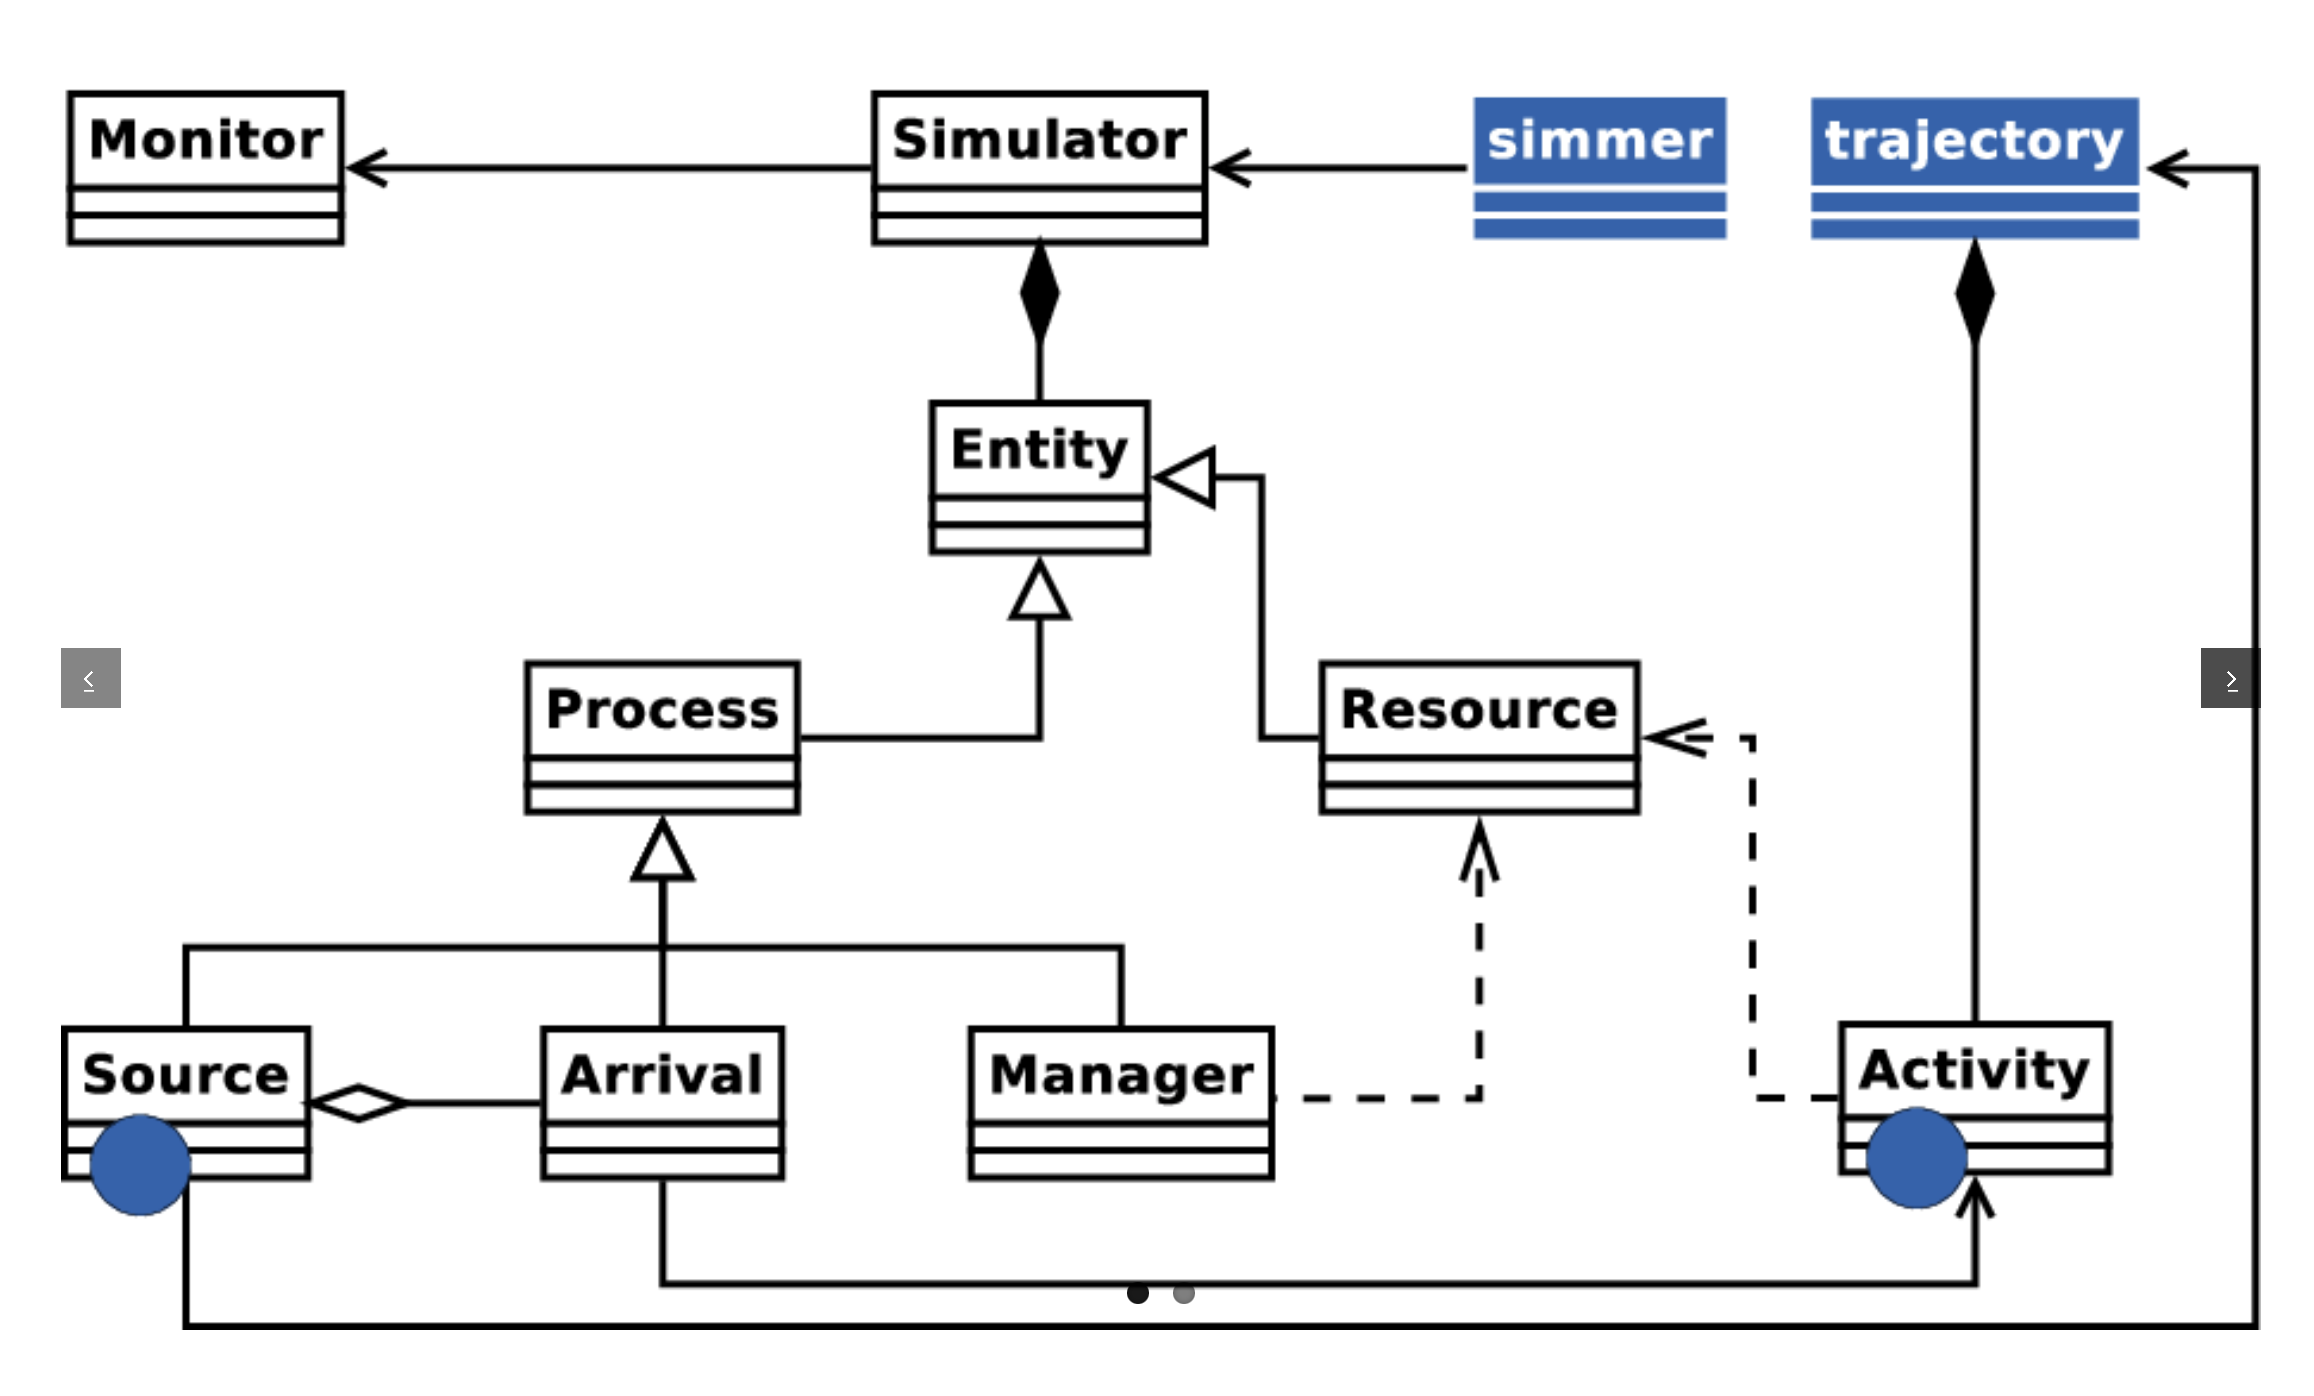
\includegraphics[width=0.8\linewidth]{images/simmer_entorno} 

}

\caption{Figura 2. Entorno de simulación en `simmer` [Fte: IBiDat](https://ibidat.es/portfolio-items/simmer-discrete-event-simulation-for-r/)}\label{fig:simmerentorno}
\end{figure}

Aunque las trayectorias se definen de modo independiente a los entornos de simulación, se recomienda definir siempre el entorno en primer lugar (pues nombra recursos y llegadas), \texttt{env=simmer()}, para luego definir las trayectorias y completar el entorno con los recursos y las fuentes. Hay que tener en cuenta que las trayectorias y los entornos van a usar elementos comunes, con lo que la sintaxis ha se ser construida y revisada en paralelo.

Para hacer correr la simulación utilizamos el comando \texttt{run()}, con el que podemos especificar cuándo parar. El comando \texttt{reset()} nos permite resetear una simulación.

Las trajectorias se pueden seccionar con el operador de selección \texttt{{[}{]}}, juntar con \texttt{join()} y modificar con el operador \texttt{=}. Hay muchas actividades disponibles en simmer para incorporar en trayectorias y que presentaremos categorizadas más adelante, según su funcionalidad.

Veamos un ejemplo de un modelo de simulación sencillo en el que llegan clientes a una tienda cada minuto (durante 3 minutos), miran los productos durante 5 minutos y se van.

\begin{Shaded}
\begin{Highlighting}[]
\NormalTok{env}\OtherTok{=}\FunctionTok{simmer}\NormalTok{()}
\CommentTok{\# Se define la trayectoria "tienda" con la actividad que realizan los clientes}
\NormalTok{tienda}\OtherTok{=}\FunctionTok{trajectory}\NormalTok{() }\SpecialCharTok{\%\textgreater{}\%}
  \CommentTok{\# Lanza un mensaje de aviso de llegada}
  \FunctionTok{log\_}\NormalTok{(}\StringTok{"Llega a la tienda"}\NormalTok{) }\SpecialCharTok{\%\textgreater{}\%}
  \CommentTok{\# mira productos 5min}
  \FunctionTok{timeout}\NormalTok{(}\DecValTok{5}\NormalTok{) }\SpecialCharTok{\%\textgreater{}\%} 
  \CommentTok{\# Lanza un mensaje de aviso de llegada}
  \FunctionTok{log\_}\NormalTok{(}\StringTok{"Sale de la tienda"}\NormalTok{)}
\CommentTok{\# se lanza el entorno de simulación incluyendo el generador de llegadas }
\CommentTok{\# (clientes), que aparecen en tres instantes de tiempo,}
\CommentTok{\# y que son dirigidos a la trayectoria "tienda"}
\NormalTok{env}\OtherTok{=}\NormalTok{env }\SpecialCharTok{\%\textgreater{}\%}
  \FunctionTok{add\_generator}\NormalTok{(}\StringTok{"cliente"}\NormalTok{, tienda,}\FunctionTok{at}\NormalTok{(}\DecValTok{1}\NormalTok{,}\DecValTok{2}\NormalTok{,}\DecValTok{3}\NormalTok{)) }\SpecialCharTok{\%\textgreater{}\%}
  \CommentTok{\# se muestran los resultados en pantalla}
  \FunctionTok{print}\NormalTok{() }\SpecialCharTok{\%\textgreater{}\%}
  \CommentTok{\# se lanza el sistema}
  \FunctionTok{run}\NormalTok{()}
\end{Highlighting}
\end{Shaded}

\begin{verbatim}
## simmer environment: anonymous | now: 0 | next: 0
## { Monitor: in memory }
## { Source: cliente | monitored: 1 | n_generated: 0 }
## 1: cliente0: Llega a la tienda
## 2: cliente1: Llega a la tienda
## 3: cliente2: Llega a la tienda
## 6: cliente0: Sale de la tienda
## 7: cliente1: Sale de la tienda
## 8: cliente2: Sale de la tienda
\end{verbatim}

Al visualizar el output, apreciamos que llegan tres clientes en los instantes 1,2,3. Cada cliente permanece en la tienda durante 5 minutos inspeccionando la mercancía, y después sale en los instantes 6, 7 y 8 respectivamente. En las actividades y generadores de llegadas hemos utilizado parámetros fijos, pero los podemos hacer aleatorios. Adaptemos el ejemplo anterior a tiempos aleatorios uniformes entre llegadas y tiempos de permanencia aleatorios normales.

\begin{Shaded}
\begin{Highlighting}[]
\NormalTok{env}\OtherTok{=}\FunctionTok{simmer}\NormalTok{()}
\NormalTok{tienda}\OtherTok{=}\FunctionTok{trajectory}\NormalTok{() }\SpecialCharTok{\%\textgreater{}\%}
  \FunctionTok{log\_}\NormalTok{(}\StringTok{"Llega a la tienda"}\NormalTok{) }\SpecialCharTok{\%\textgreater{}\%}
  \CommentTok{\# Cada cliente permanece en la tienda mirando productos aprox. 5min}
  \FunctionTok{timeout}\NormalTok{(}\ControlFlowTok{function}\NormalTok{() }\FunctionTok{rnorm}\NormalTok{(}\DecValTok{1}\NormalTok{,}\DecValTok{5}\NormalTok{,}\DecValTok{1}\NormalTok{)) }\SpecialCharTok{\%\textgreater{}\%} 
  \FunctionTok{log\_}\NormalTok{(}\StringTok{"Sale de la tienda"}\NormalTok{)}

\NormalTok{env}\OtherTok{=}\NormalTok{env }\SpecialCharTok{\%\textgreater{}\%}
  \CommentTok{\# el tiempo entre llegadas de los clientes es aleatorio entre 0 y 2 min.}
  \FunctionTok{add\_generator}\NormalTok{(}\StringTok{"cliente"}\NormalTok{, tienda,}\ControlFlowTok{function}\NormalTok{() }\FunctionTok{runif}\NormalTok{(}\DecValTok{1}\NormalTok{,}\DecValTok{0}\NormalTok{,}\DecValTok{2}\NormalTok{)) }\SpecialCharTok{\%\textgreater{}\%} 
  \FunctionTok{print}\NormalTok{() }\SpecialCharTok{\%\textgreater{}\%}
  \CommentTok{\# simulamos hasta el instante 10}
  \FunctionTok{run}\NormalTok{(}\DecValTok{10}\NormalTok{) }
\end{Highlighting}
\end{Shaded}

\begin{verbatim}
## simmer environment: anonymous | now: 0 | next: 0
## { Monitor: in memory }
## { Source: cliente | monitored: 1 | n_generated: 0 }
## 1.20152: cliente0: Llega a la tienda
## 1.51594: cliente1: Llega a la tienda
## 2.51149: cliente2: Llega a la tienda
## 3.76426: cliente0: Sale de la tienda
## 4.05654: cliente3: Llega a la tienda
## 4.12502: cliente4: Llega a la tienda
## 4.51636: cliente5: Llega a la tienda
## 5.29376: cliente6: Llega a la tienda
## 5.96187: cliente1: Sale de la tienda
## 6.65052: cliente7: Llega a la tienda
## 8.58992: cliente3: Sale de la tienda
## 8.6116: cliente8: Llega a la tienda
## 8.65991: cliente2: Sale de la tienda
## 8.88082: cliente4: Sale de la tienda
## 9.67203: cliente9: Llega a la tienda
## 9.73449: cliente10: Llega a la tienda
\end{verbatim}

Ahora vemos en la primera columna los instantes de tiempo en que llegan y se van los clientes.

\hypertarget{recursos}{%
\subsection{Recursos}\label{recursos}}

Recordemos que un recurso, que proporciona servicio a las llegadas, en la simulación DES tiene dos componentes internos: un servidor y una cola. Todo recurso va a ser definido por tres parámetros:

\begin{itemize}
\tightlist
\item
  el nombre (\emph{name}) del recurso o servidor,
\item
  la capacidad (\emph{capacity}) del recurso, y
\item
  el tamaño de la cola (\emph{queue\_size}) en la que esperan las llegadas a que haya algún recurso disponible; representa el aforo de la sala de espera; cuando es cero significa que no hay posibilidad de cola.
\end{itemize}

Los recursos se definen con la sintaxis:

\begin{verbatim}
add_resource(.env, name, capacity = 1, queue_size = Inf, mon = TRUE,
  preemptive = FALSE, preempt_order = c("fifo", "lifo"),
  queue_size_strict = FALSE, queue_priority = c(0, Inf))
\end{verbatim}

El argumento \texttt{capacity} indica cuántos servidores hay en el sistema, y \texttt{queue\_size} el tamaño de la cola de espera. Por defecto, los recursos son monitorizados (\texttt{mon=TRUE}) y no preferentes (\texttt{preemptive\ =\ FALSE}). La preferencia significa que si aparece una llegada con prioridad alta, el recurso detendrá temporalmente el procesado de las llegadas que esté atendiendo y tengan menos prioridad, y atenderá la preferente. En los recursos preferentes, \texttt{preemptive\ =\ TRUE} el parámetro \texttt{preempt\_order} define qué llegada debe priorizarse según una política FIFO (\emph{First in, first out})o LIFO (\emph{Last in, first out}). Todas las llegadas con mayor preferencia son ubicadas en una cola especial que tiene mayor prioridad que la cola principal, y en consecuencia se atienden antes. Además, el parámetro \texttt{queue\_size\_strict} controla si esta cola especial de llegadas preferentes debe ser tenida en cuenta para calcular el tamaño límite de la cola; si este parámetro impone el límite, entonces los rechazos se producirán en la cola principal.

Para ampliar información, consultar el Manual de Referencia sobre \href{https://r-simmer.org/reference/add_resource.html}{\texttt{add\_resource}}.

Cuando tenemos recursos en el sistema que dan un servicio, surgen dos acciones básicas que son: \texttt{seize} o asignación a un recurso, y \texttt{release} o desocupación del recurso. Por supuesto, si una llegada no puede ser atendida por un servidor (recurso) libre, puede esperar en cola si hay hueco en la cola, o ser rechazada si no lo hay.

Transformemos el ejemplo anterior en clientes que llegan aleatoriamente a una tienda. Ahora al llegar, cada cliente mira productos alrededor de 5 minutos, luego busca a un dependiente para ser atendido o espera hasta que uno esté desocupado, este lo atiende por aproximadamente 10 minutos y luego se va. Supongamos que hay 2 dependientes en la tienda.

\begin{Shaded}
\begin{Highlighting}[]
\FunctionTok{set.seed}\NormalTok{(}\DecValTok{999}\NormalTok{)}
\NormalTok{env}\OtherTok{=}\FunctionTok{simmer}\NormalTok{()}

\CommentTok{\# Actividades que se desarrollan en la tienda}
\NormalTok{tienda}\OtherTok{=}\FunctionTok{trajectory}\NormalTok{() }\SpecialCharTok{\%\textgreater{}\%}
  \FunctionTok{log\_}\NormalTok{(}\ControlFlowTok{function}\NormalTok{()  }\StringTok{"Llega a la tienda"}\NormalTok{) }\SpecialCharTok{\%\textgreater{}\%}
  \CommentTok{\# mira productos aprox. 5min}
  \FunctionTok{timeout}\NormalTok{(}\ControlFlowTok{function}\NormalTok{() }\FunctionTok{rnorm}\NormalTok{(}\DecValTok{1}\NormalTok{,}\DecValTok{5}\NormalTok{,}\DecValTok{1}\NormalTok{)) }\SpecialCharTok{\%\textgreater{}\%} 
  \CommentTok{\# es asignado a un dependiente }
  \FunctionTok{log\_}\NormalTok{(}\ControlFlowTok{function}\NormalTok{() }\StringTok{"Busca un dependiente"}\NormalTok{) }\SpecialCharTok{\%\textgreater{}\%}
  \FunctionTok{seize}\NormalTok{(}\StringTok{"dependiente"}\NormalTok{,}\DecValTok{1}\NormalTok{) }\SpecialCharTok{\%\textgreater{}\%}
  \CommentTok{\# que lo antiende aprox. 10min.}
  \FunctionTok{log\_}\NormalTok{(}\StringTok{"Es atendido"}\NormalTok{) }\SpecialCharTok{\%\textgreater{}\%}
  \FunctionTok{timeout}\NormalTok{(}\ControlFlowTok{function}\NormalTok{() }\FunctionTok{rnorm}\NormalTok{(}\DecValTok{1}\NormalTok{,}\DecValTok{10}\NormalTok{,}\DecValTok{1}\NormalTok{)) }\SpecialCharTok{\%\textgreater{}\%}
  \CommentTok{\# desocupa al dependiente}
  \FunctionTok{release}\NormalTok{(}\StringTok{"dependiente"}\NormalTok{,}\DecValTok{1}\NormalTok{)}\SpecialCharTok{\%\textgreater{}\%}
  \CommentTok{\# sale de la tienda}
  \FunctionTok{log\_}\NormalTok{(}\ControlFlowTok{function}\NormalTok{() }\StringTok{"Sale de la tienda"}\NormalTok{)}

\NormalTok{env}\OtherTok{=}\NormalTok{env }\SpecialCharTok{\%\textgreater{}\%}
  \CommentTok{\# simulación (uniforme(0,5) del tiempo entre llegadas de clientes}
  \FunctionTok{add\_generator}\NormalTok{(}\StringTok{"cliente"}\NormalTok{, tienda,}\ControlFlowTok{function}\NormalTok{() }\FunctionTok{runif}\NormalTok{(}\DecValTok{1}\NormalTok{,}\DecValTok{0}\NormalTok{,}\DecValTok{5}\NormalTok{)) }\SpecialCharTok{\%\textgreater{}\%} 
  \CommentTok{\# dimensionamiento de recursos: dos dependientes}
  \FunctionTok{add\_resource}\NormalTok{(}\StringTok{"dependiente"}\NormalTok{,}\DecValTok{2}\NormalTok{) }\SpecialCharTok{\%\textgreater{}\%}  
  \FunctionTok{print}\NormalTok{() }\SpecialCharTok{\%\textgreater{}\%}
  \FunctionTok{run}\NormalTok{(}\DecValTok{20}\NormalTok{) }\SpecialCharTok{\%\textgreater{}\%} \CommentTok{\# simulamos hasta ese instante}
  \CommentTok{\# monitorizamos los recursos (dependientes)}
  \FunctionTok{get\_mon\_resources}\NormalTok{()}
\end{Highlighting}
\end{Shaded}

\begin{verbatim}
## simmer environment: anonymous | now: 0 | next: 0
## { Monitor: in memory }
## { Resource: dependiente | monitored: TRUE | server status: 0(2) | queue status: 0(Inf) }
## { Source: cliente | monitored: 1 | n_generated: 0 }
## 1.94536: cliente0: Llega a la tienda
## 4.86066: cliente1: Llega a la tienda
## 5.6328: cliente0: Busca un dependiente
## 5.6328: cliente0: Es atendido
## 8.68238: cliente1: Busca un dependiente
## 8.68238: cliente1: Es atendido
## 8.79439: cliente2: Llega a la tienda
## 11.55: cliente3: Llega a la tienda
## 11.9157: cliente2: Busca un dependiente
## 12.0631: cliente4: Llega a la tienda
## 14.2341: cliente0: Sale de la tienda
## 14.2341: cliente2: Es atendido
## 15.9421: cliente4: Busca un dependiente
## 16.1694: cliente5: Llega a la tienda
## 17.3468: cliente3: Busca un dependiente
## 18.9358: cliente6: Llega a la tienda
## 18.9865: cliente1: Sale de la tienda
## 18.9865: cliente4: Es atendido
\end{verbatim}

Visualizamos a los clientes: cuándo llegan, cuándo son atendidos por un dependiente y cuándo se van de la tienda. Para los dependientes (recursos) vemos los instantes de tiempo (time) en los que inician un servicio o se les añade algún cliente en cola, el número de dependientes ocupados (server) y el número de clientes esperando ser atendidos (queue).

\hypertarget{fuentes}{%
\subsection{Fuentes}\label{fuentes}}

Una fuente de llegadas, clientes o productos de un sistema de simulación es definida con tres parámetros principales:

\begin{itemize}
\tightlist
\item
  \emph{name\_prefix}, el nombre con el que identificamos cada llegada que se genera
\item
  \emph{trajectory}, la trayectoria a la que accede
\item
  \emph{distribution}, la distribución de los tiempos entre llegadas.
\end{itemize}

Hay dos tipos de fuentes: generadores y fuentes de datos (\emph{dataframes}), a las que accedemos respectivamente con los comandos \texttt{add\_generator()} y \texttt{add\_dataframe()}.

\begin{itemize}
\tightlist
\item
  \textbf{Generadores}, proporcionados con el comando \texttt{add\_generator()}, que genera tiempos dinámicos entre llegadas a partir de una función (distribución) que define el usuario.
\end{itemize}

Ejemplifiquemos las posibilidades de generación de tiempos de llegadas con el ejemplo anterior que ya realizamos, en el que al entrar cada cliente, pasa 5 minutos en el sistema y luego se marcha.

\begin{Shaded}
\begin{Highlighting}[]
\NormalTok{env}\OtherTok{=}\FunctionTok{simmer}\NormalTok{()}
\CommentTok{\# defino la función de los tiempos entre llegadas, U(0,2)}
\NormalTok{distr }\OtherTok{\textless{}{-}} \ControlFlowTok{function}\NormalTok{() }\FunctionTok{runif}\NormalTok{(}\DecValTok{1}\NormalTok{, }\DecValTok{0}\NormalTok{, }\DecValTok{2}\NormalTok{)}

\CommentTok{\# definimos laa acciones que hace el cliente en la tienda}
\NormalTok{tienda }\OtherTok{\textless{}{-}} \FunctionTok{trajectory}\NormalTok{() }\SpecialCharTok{\%\textgreater{}\%}
  \FunctionTok{timeout}\NormalTok{(}\DecValTok{5}\NormalTok{)}

\NormalTok{env }\SpecialCharTok{\%\textgreater{}\%}
  \CommentTok{\# los tiempos entre llegadas se simulan de "distr"}
  \FunctionTok{add\_generator}\NormalTok{(}\StringTok{"llegada\_random"}\NormalTok{, tienda, distr) }\SpecialCharTok{\%\textgreater{}\%}
  \CommentTok{\# las llegadas ocurren en los instantes 0, 1, 10, 30, 40 y 43}
  \FunctionTok{add\_generator}\NormalTok{(}\StringTok{"llegada\_at"}\NormalTok{, tienda, }\FunctionTok{at}\NormalTok{(}\DecValTok{0}\NormalTok{,}\DecValTok{1}\NormalTok{,}\DecValTok{10}\NormalTok{,}\DecValTok{30}\NormalTok{,}\DecValTok{40}\NormalTok{,}\DecValTok{43}\NormalTok{)) }\SpecialCharTok{\%\textgreater{}\%}
  \CommentTok{\# los tiempos entre llegadas se simulan de "distr", empezando en el instante 1}
  \FunctionTok{add\_generator}\NormalTok{(}\StringTok{"llegada\_from"}\NormalTok{, tienda, }\FunctionTok{from}\NormalTok{(}\DecValTok{1}\NormalTok{, distr)) }\SpecialCharTok{\%\textgreater{}\%}
  \CommentTok{\# los tiempos entre llegadas se simulan de "distr", acabando en el instante 5}
  \FunctionTok{add\_generator}\NormalTok{(}\StringTok{"llegada\_to"}\NormalTok{, tienda, }\FunctionTok{to}\NormalTok{(}\DecValTok{5}\NormalTok{, distr)) }\SpecialCharTok{\%\textgreater{}\%}
  \CommentTok{\# los tiempos entre llegadas se simulan de "distr", empezando en 1 y acabando en 5}
  \FunctionTok{add\_generator}\NormalTok{(}\StringTok{"llegada\_from\_to"}\NormalTok{, tienda, }\FunctionTok{from\_to}\NormalTok{(}\DecValTok{1}\NormalTok{, }\DecValTok{5}\NormalTok{, distr, }\AttributeTok{every=}\DecValTok{4}\NormalTok{)) }\SpecialCharTok{\%\textgreater{}\%}
  \FunctionTok{run}\NormalTok{(}\DecValTok{15}\NormalTok{) }\SpecialCharTok{\%\textgreater{}\%} 
  \CommentTok{\# monitorizamos todas las llegadas}
  \FunctionTok{get\_mon\_arrivals}\NormalTok{()}
\end{Highlighting}
\end{Shaded}

\begin{verbatim}
##                name start_time  end_time activity_time finished replication
## 1       llegada_at0  0.0000000  5.000000             5     TRUE           1
## 2   llegada_random0  0.1729814  5.172981             5     TRUE           1
## 3       llegada_to0  0.4509553  5.450955             5     TRUE           1
## 4       llegada_at1  1.0000000  6.000000             5     TRUE           1
## 5     llegada_from0  1.0000000  6.000000             5     TRUE           1
## 6  llegada_from_to0  1.0000000  6.000000             5     TRUE           1
## 7   llegada_random1  1.2274626  6.227463             5     TRUE           1
## 8       llegada_to1  1.6187369  6.618737             5     TRUE           1
## 9     llegada_from1  2.0801778  7.080178             5     TRUE           1
## 10    llegada_from2  2.1182239  7.118224             5     TRUE           1
## 11 llegada_from_to1  2.7380298  7.738030             5     TRUE           1
## 12  llegada_random2  2.8600575  7.860058             5     TRUE           1
## 13 llegada_from_to2  2.9572654  7.957265             5     TRUE           1
## 14    llegada_from3  2.9890172  7.989017             5     TRUE           1
## 15      llegada_to2  3.1719196  8.171920             5     TRUE           1
## 16      llegada_to3  3.8909441  8.890944             5     TRUE           1
## 17    llegada_from4  3.9343827  8.934383             5     TRUE           1
## 18 llegada_from_to3  4.4370700  9.437070             5     TRUE           1
## 19      llegada_to4  4.4642147  9.464215             5     TRUE           1
## 20  llegada_random3  4.4702904  9.470290             5     TRUE           1
## 21  llegada_random4  4.5808807  9.580881             5     TRUE           1
## 22      llegada_to5  4.7246900  9.724690             5     TRUE           1
## 23 llegada_from_to4  4.9288147  9.928815             5     TRUE           1
## 24 llegada_from_to5  5.0000000 10.000000             5     TRUE           1
## 25    llegada_from5  5.1656520 10.165652             5     TRUE           1
## 26    llegada_from6  5.5418947 10.541895             5     TRUE           1
## 27  llegada_random5  6.0601800 11.060180             5     TRUE           1
## 28  llegada_random6  6.1803417 11.180342             5     TRUE           1
## 29    llegada_from7  6.7354383 11.735438             5     TRUE           1
## 30 llegada_from_to6  6.7442407 11.744241             5     TRUE           1
## 31    llegada_from8  7.6346328 12.634633             5     TRUE           1
## 32  llegada_random7  7.6924460 12.692446             5     TRUE           1
## 33 llegada_from_to7  8.4122507 13.412251             5     TRUE           1
## 34 llegada_from_to8  9.0000000 14.000000             5     TRUE           1
## 35  llegada_random8  9.2487709 14.248771             5     TRUE           1
## 36    llegada_from9  9.6174449 14.617445             5     TRUE           1
\end{verbatim}

También podemos desencadenar llegadas a demanda desde otra trayectoria. Sería el ejemplo de un operador, que en el momento en que ficha digitalmente como trabajador de la empresa, se incorpora a trabajar durante una jornada parcial de 3 horas:

\begin{Shaded}
\begin{Highlighting}[]
\CommentTok{\# jornada de trabajo}
\NormalTok{t0 }\OtherTok{\textless{}{-}} \FunctionTok{trajectory}\NormalTok{() }\SpecialCharTok{\%\textgreater{}\%}
  \FunctionTok{timeout}\NormalTok{(}\DecValTok{3}\NormalTok{)}
\CommentTok{\# activa "Trabajar": la jornada de trabajo}
\NormalTok{t1 }\OtherTok{\textless{}{-}} \FunctionTok{trajectory}\NormalTok{() }\SpecialCharTok{\%\textgreater{}\%}
  \FunctionTok{activate}\NormalTok{(}\StringTok{"Trabajar"}\NormalTok{)}

\FunctionTok{simmer}\NormalTok{() }\SpecialCharTok{\%\textgreater{}\%}
  \CommentTok{\# simula llegadas al trabajo cuando "Trabajar" esté activado}
  \FunctionTok{add\_generator}\NormalTok{(}\StringTok{"Trabajar"}\NormalTok{, t0, }\FunctionTok{when\_activated}\NormalTok{()) }\SpecialCharTok{\%\textgreater{}\%}
  \CommentTok{\# simula una llegada a fichar}
  \FunctionTok{add\_generator}\NormalTok{(}\StringTok{"Fichado digital"}\NormalTok{, t1, }\FunctionTok{at}\NormalTok{(}\DecValTok{8}\NormalTok{)) }\SpecialCharTok{\%\textgreater{}\%}
  \FunctionTok{run}\NormalTok{() }\SpecialCharTok{\%\textgreater{}\%}
  \FunctionTok{get\_mon\_arrivals}\NormalTok{()}
\end{Highlighting}
\end{Shaded}

\begin{verbatim}
##               name start_time end_time activity_time finished replication
## 1 Fichado digital0          8        8             0     TRUE           1
## 2        Trabajar0          8       11             3     TRUE           1
\end{verbatim}

La sintaxis que se utiliza para generar llegadas es:

\begin{verbatim}
add_generator(.env, name_prefix, trajectory, distribution, mon = 1,
  priority = 0, preemptible = priority, restart = FALSE)
\end{verbatim}

El argumento \texttt{mon} permite especificar si queremos que el simulador monitoree las llegadas: 0 = sin monitoreo, 1 = monitoreo simple de llegadas simple, 2 = monitoreo simple y de atributos de las llegadas. Por defecto tendremos \texttt{mon=1}. En el argumento \texttt{distribution} se pueden utilizar funciones definidas por el usuario para los tiempos entre llegadas y también, como hemos visto, \texttt{at()}, \texttt{from()}, \texttt{to()} y \texttt{from\_to()}. Si hay un sistema de prioridades, se especificaría con \texttt{priority=1}, y qué hacer para las llegadas preferentes o prioritarias, en los argumentos \texttt{preemptible} y \texttt{restart}.

Para ampliar información, consultar el Manual de Referencia sobre \href{https://r-simmer.org/reference/generators.html}{\texttt{add\_generator}}.

\begin{itemize}
\tightlist
\item
  \textbf{Fuentes de datos} con tiempos entre llegadas, provenientes de un data frame que vincula el usuario con el comando \texttt{add\_dataframe()}:
\end{itemize}

\begin{verbatim}
add_dataframe(.env, name_prefix, trajectory, data, mon = 1, batch = 50,
  col_time = "time", time = c("interarrival", "absolute"),
  col_attributes = NULL, col_priority = "priority",
  col_preemptible = col_priority, col_restart = "restart")
\end{verbatim}

Ambos generadores o fuentes de llegadas se reprograman a sí mismos para ciclarse hasta agotar el tiempo de simulación, en el caso de que este supere el rango inicial.

Para ampliar información, consultar el Manual de Referencia sobre \href{https://r-simmer.org/reference/add_generator.html}{\texttt{add\_generator}} y \href{https://r-simmer.org/reference/add_dataframe.html}{\texttt{add\_dataframe}}.

\hypertarget{atributos}{%
\subsection{Atributos}\label{atributos}}

Falta por completar información.

\hypertarget{monitoreo}{%
\subsection{Monitoreo}\label{monitoreo}}

Al ejecutar un entorno de simulación, si no incluimos ninguna opción de visualización de mensajes en la trayectoria, obtenemos en pantalla un resumen escrito básico sobre recursos y llegadas.

\begin{Shaded}
\begin{Highlighting}[]
\NormalTok{trayectoria}\OtherTok{=}\FunctionTok{trajectory}\NormalTok{() }\SpecialCharTok{\%\textgreater{}\%}
   \FunctionTok{timeout}\NormalTok{(}\DecValTok{3}\NormalTok{)}

\FunctionTok{simmer}\NormalTok{() }\SpecialCharTok{\%\textgreater{}\%}
  \FunctionTok{add\_generator}\NormalTok{(}\StringTok{"llegada"}\NormalTok{,trayectoria,}\FunctionTok{at}\NormalTok{(}\DecValTok{0}\NormalTok{,}\DecValTok{1}\NormalTok{,}\DecValTok{2}\NormalTok{)) }\SpecialCharTok{\%\textgreater{}\%}
  \FunctionTok{run}\NormalTok{() }
\end{Highlighting}
\end{Shaded}

\begin{verbatim}
## simmer environment: anonymous | now: 5 | next: 
## { Monitor: in memory }
## { Source: llegada | monitored: 1 | n_generated: 3 }
\end{verbatim}

Al añadir en la ejecución del entorno el comando \texttt{print()} (antes de \texttt{run()}), se monitorizan los eventos que se van sucediendo en la simulación y dónde se almacenan (Monitor).

\begin{Shaded}
\begin{Highlighting}[]
\FunctionTok{simmer}\NormalTok{() }\SpecialCharTok{\%\textgreater{}\%}
  \FunctionTok{add\_generator}\NormalTok{(}\StringTok{"llegada"}\NormalTok{,trayectoria,}\FunctionTok{at}\NormalTok{(}\DecValTok{0}\NormalTok{,}\DecValTok{1}\NormalTok{,}\DecValTok{2}\NormalTok{)) }\SpecialCharTok{\%\textgreater{}\%}
  \FunctionTok{print}\NormalTok{() }\SpecialCharTok{\%\textgreater{}\%}
  \FunctionTok{run}\NormalTok{() }
\end{Highlighting}
\end{Shaded}

\begin{verbatim}
## simmer environment: anonymous | now: 0 | next: 0
## { Monitor: in memory }
## { Source: llegada | monitored: 1 | n_generated: 0 }
\end{verbatim}

\begin{verbatim}
## simmer environment: anonymous | now: 5 | next: 
## { Monitor: in memory }
## { Source: llegada | monitored: 1 | n_generated: 3 }
\end{verbatim}

El comando \texttt{invisible} (después de \texttt{run()}) depura la salida para no visualizar nada (salvo que hayamos incorporado mensajes en las trayectorias).

\begin{Shaded}
\begin{Highlighting}[]
\FunctionTok{simmer}\NormalTok{() }\SpecialCharTok{\%\textgreater{}\%}
  \FunctionTok{add\_generator}\NormalTok{(}\StringTok{"llegada"}\NormalTok{,trayectoria,}\FunctionTok{at}\NormalTok{(}\DecValTok{0}\NormalTok{,}\DecValTok{1}\NormalTok{,}\DecValTok{2}\NormalTok{)) }\SpecialCharTok{\%\textgreater{}\%}
  \FunctionTok{run}\NormalTok{() }\SpecialCharTok{\%\textgreater{}\%}
\NormalTok{  invisible}
\end{Highlighting}
\end{Shaded}

Si queremos visualizar mensajes específicos vinculados a las llegadas y actividades conforme se suceden, habremos de incluir mensajes en las trayectorias a través del comando \texttt{log\_()}.

\begin{Shaded}
\begin{Highlighting}[]
\NormalTok{env}\OtherTok{=}\FunctionTok{simmer}\NormalTok{()}
\NormalTok{trayectoria}\OtherTok{=}\FunctionTok{trajectory}\NormalTok{() }\SpecialCharTok{\%\textgreater{}\%}
  \FunctionTok{log\_}\NormalTok{(}\StringTok{"Llegada contabilizada."}\NormalTok{) }\SpecialCharTok{\%\textgreater{}\%}
  \FunctionTok{timeout}\NormalTok{(}\DecValTok{3}\NormalTok{)}

\NormalTok{env}\OtherTok{=}\NormalTok{env }\SpecialCharTok{\%\textgreater{}\%}
  \FunctionTok{add\_generator}\NormalTok{(}\StringTok{"llegada"}\NormalTok{,trayectoria,}\ControlFlowTok{function}\NormalTok{() }\FunctionTok{rexp}\NormalTok{(}\DecValTok{1}\NormalTok{,}\DecValTok{1}\SpecialCharTok{/}\DecValTok{2}\NormalTok{)) }\SpecialCharTok{\%\textgreater{}\%}
  \FunctionTok{run}\NormalTok{(}\DecValTok{5}\NormalTok{) }\SpecialCharTok{\%\textgreater{}\%}
\NormalTok{  invisible}
\end{Highlighting}
\end{Shaded}

Una vez lanzamos un sistema de simulación, disponemos de diversos métodos para extraer información de él y monitorizarla por ejemplo con el comando \texttt{log\_()}:

\begin{itemize}
\tightlist
\item
  \texttt{now()} el tiempo de simulación actual
\item
  \texttt{peek(n)} instantes de tiempo en los que acontecerán los siguientes \(n\) eventos
\item
  \texttt{get\_*()} para obtener información de recursos, atributos y fuentes: \texttt{attribute}, \texttt{capacity}, \texttt{global}, \texttt{name}, \texttt{n\_activities}, \texttt{n\_generated}, \texttt{prioritization}, \texttt{queue\_count}, \texttt{queue\_size}, \texttt{resources}, \texttt{seized}, \texttt{server\_count}, \texttt{sources}, \texttt{trajectory}.
\end{itemize}

\begin{Shaded}
\begin{Highlighting}[]
\NormalTok{env }\SpecialCharTok{\%\textgreater{}\%}
    \FunctionTok{peek}\NormalTok{(}\DecValTok{3}\NormalTok{)}
\end{Highlighting}
\end{Shaded}

\begin{verbatim}
## [1] 5.35573 5.35573
\end{verbatim}

Con el comando \texttt{stepn()} podemos hacer correr el sistema durante una única simulación adicional, que no se almacena en el objeto de simulación salvo que lo asignemos a él.

\begin{Shaded}
\begin{Highlighting}[]
\NormalTok{env}\OtherTok{=}\NormalTok{env }\SpecialCharTok{\%\textgreater{}\%}
  \FunctionTok{stepn}\NormalTok{() }\SpecialCharTok{\%\textgreater{}\%}
  \FunctionTok{print}\NormalTok{()}
\end{Highlighting}
\end{Shaded}

\begin{verbatim}
## 5.35573: llegada0: Llegada contabilizada.
## simmer environment: anonymous | now: 5.35572961320109 | next: 5.35572961320109
## { Monitor: in memory }
## { Source: llegada | monitored: 1 | n_generated: 1 }
\end{verbatim}

Los comandos para monitorizar se pueden aplicar a un único entorno de simulación o a una lista de entornos, y el objeto de retorno es siempre un data frame, incluso si no se encuentran datos. Cada entorno de simulación procesado se trata como una replicación diferente, y se identifica como tal en una columna numérica denominada \emph{replication} en el dataframe de retorno, con los índices de los entornos como valores. Recuperamos llegadas, recursos y atributos del sistema con los comandos:

\begin{itemize}
\item
  \texttt{get\_mon\_arrivals()} devuelve la información temporal por llegada: nombre (\emph{name}) de la llegada, tiempo de llegada (\emph{start\_time}), tiempo de salida (\emph{end\_time}), tiempo en la actividad sin estar en la cola (\emph{activity\_time}) y una etiqueta \emph{finished} que indica si la llegada finalizó sus actividades. Por defecto esta información se refiere al tiempo de vida completo de las llegadas, pero se puede obtener por recurso con el argumento \texttt{per\_resource=TRUE}.
\item
  \texttt{get\_mon\_resources()} devuelve los cambios de estado en los recursos: nombre del recurso (\emph{resource}), instante (\emph{time}) del evento que desencadenó el cambio de estado, contador de unidades en servicio (\emph{server}), contador de unidades en la cola (\emph{queue}), capacidad (\emph{capacity}), tamaño de la cola (\emph{queue\_size}), contador del sistema (\emph{system=server+queue}), y límite del sistema (\emph{limit=capacity+queue\_size}).
\item
  \texttt{get\_mon\_atributes()} devuelve los cambios de estado en los atributos: nombre (\emph{name}) del atributo, instante (\emph{time}) del evento que desencadenó el cambio de estado, nombre (\emph{key}) que identifica el atributo y valor (\emph{value}).
\end{itemize}

\begin{verbatim}
llegadas=get_mon_arrivals(env) 
llegadas
atributos=get_mon_attributes(env)
atributos
recursos=get_mon_resources(env)
recursos
\end{verbatim}

Ejemplifiquemos su funcionamiento sobre el sistema sencillo de la tienda que ya vimos anteriormente, con tiempos para mirar al llegar a la tienda, seguidos de atención por dependientes.

\begin{Shaded}
\begin{Highlighting}[]
\NormalTok{env}\OtherTok{=}\FunctionTok{simmer}\NormalTok{()}
\NormalTok{tienda}\OtherTok{=}\FunctionTok{trajectory}\NormalTok{() }\SpecialCharTok{\%\textgreater{}\%}
  \FunctionTok{log\_}\NormalTok{(}\ControlFlowTok{function}\NormalTok{()  }\StringTok{"Llega a la tienda"}\NormalTok{) }\SpecialCharTok{\%\textgreater{}\%}
  \FunctionTok{timeout}\NormalTok{(}\ControlFlowTok{function}\NormalTok{() }\FunctionTok{rnorm}\NormalTok{(}\DecValTok{1}\NormalTok{,}\DecValTok{5}\NormalTok{,}\DecValTok{1}\NormalTok{)) }\SpecialCharTok{\%\textgreater{}\%} \CommentTok{\# mira productos aprox. 5min}
  \FunctionTok{seize}\NormalTok{(}\StringTok{"dependiente"}\NormalTok{,}\DecValTok{1}\NormalTok{) }\SpecialCharTok{\%\textgreater{}\%}
  \FunctionTok{log\_}\NormalTok{(}\StringTok{"Es atendido"}\NormalTok{) }\SpecialCharTok{\%\textgreater{}\%}
  \FunctionTok{timeout}\NormalTok{(}\ControlFlowTok{function}\NormalTok{() }\FunctionTok{rnorm}\NormalTok{(}\DecValTok{1}\NormalTok{,}\DecValTok{10}\NormalTok{,}\DecValTok{1}\NormalTok{)) }\SpecialCharTok{\%\textgreater{}\%}
  \FunctionTok{release}\NormalTok{(}\StringTok{"dependiente"}\NormalTok{,}\DecValTok{1}\NormalTok{)}\SpecialCharTok{\%\textgreater{}\%}
  \FunctionTok{log\_}\NormalTok{(}\ControlFlowTok{function}\NormalTok{() }\StringTok{"Sale de la tienda"}\NormalTok{)}

\NormalTok{env}\OtherTok{=}\NormalTok{env }\SpecialCharTok{\%\textgreater{}\%}
  \FunctionTok{add\_generator}\NormalTok{(}\StringTok{"cliente"}\NormalTok{, tienda,}\ControlFlowTok{function}\NormalTok{() }\FunctionTok{runif}\NormalTok{(}\DecValTok{1}\NormalTok{,}\DecValTok{0}\NormalTok{,}\DecValTok{5}\NormalTok{)) }\SpecialCharTok{\%\textgreater{}\%} \CommentTok{\# tiempo entre llegadas }
  \FunctionTok{add\_resource}\NormalTok{(}\StringTok{"dependiente"}\NormalTok{,}\DecValTok{2}\NormalTok{) }\SpecialCharTok{\%\textgreater{}\%} \CommentTok{\# hay dos dependientes}
  \FunctionTok{print}\NormalTok{() }\SpecialCharTok{\%\textgreater{}\%}
  \FunctionTok{run}\NormalTok{(}\DecValTok{20}\NormalTok{) }\CommentTok{\# simulamos hasta ese instante}
\end{Highlighting}
\end{Shaded}

\begin{verbatim}
## simmer environment: anonymous | now: 0 | next: 0
## { Monitor: in memory }
## { Resource: dependiente | monitored: TRUE | server status: 0(2) | queue status: 0(Inf) }
## { Source: cliente | monitored: 1 | n_generated: 0 }
## 1.13087: cliente0: Llega a la tienda
## 1.79667: cliente1: Llega a la tienda
## 4.27508: cliente2: Llega a la tienda
## 4.37577: cliente3: Llega a la tienda
## 5.20351: cliente4: Llega a la tienda
## 7.07315: cliente1: Es atendido
## 7.63425: cliente5: Llega a la tienda
## 7.96535: cliente0: Es atendido
## 12.2561: cliente6: Llega a la tienda
## 14.623: cliente7: Llega a la tienda
## 15.7281: cliente8: Llega a la tienda
## 16.2301: cliente9: Llega a la tienda
## 16.297: cliente10: Llega a la tienda
## 17.1866: cliente11: Llega a la tienda
## 17.6022: cliente12: Llega a la tienda
## 18.3314: cliente0: Sale de la tienda
## 18.3314: cliente2: Es atendido
## 18.7997: cliente1: Sale de la tienda
## 18.7997: cliente3: Es atendido
\end{verbatim}

\begin{Shaded}
\begin{Highlighting}[]
\NormalTok{llegadas}\OtherTok{=}\FunctionTok{get\_mon\_arrivals}\NormalTok{(env) }
\NormalTok{llegadas}
\end{Highlighting}
\end{Shaded}

\begin{verbatim}
##       name start_time end_time activity_time finished replication
## 1 cliente0   1.130873 18.33144      17.20057     TRUE           1
## 2 cliente1   1.796671 18.79968      17.00301     TRUE           1
\end{verbatim}

\begin{Shaded}
\begin{Highlighting}[]
\NormalTok{atributos}\OtherTok{=}\FunctionTok{get\_mon\_attributes}\NormalTok{(env)}
\NormalTok{atributos}
\end{Highlighting}
\end{Shaded}

\begin{verbatim}
## [1] time  name  key   value
## <0 rows> (or 0-length row.names)
\end{verbatim}

\begin{Shaded}
\begin{Highlighting}[]
\NormalTok{recursos}\OtherTok{=}\FunctionTok{get\_mon\_resources}\NormalTok{(env)}
\NormalTok{recursos}
\end{Highlighting}
\end{Shaded}

\begin{verbatim}
##      resource      time server queue capacity queue_size system limit replication
## 1 dependiente  7.073150      1     0        2        Inf      1   Inf           1
## 2 dependiente  7.965346      2     0        2        Inf      2   Inf           1
## 3 dependiente  9.788494      2     1        2        Inf      3   Inf           1
## 4 dependiente  9.958040      2     2        2        Inf      4   Inf           1
## 5 dependiente 11.436010      2     3        2        Inf      5   Inf           1
## 6 dependiente 14.378664      2     4        2        Inf      6   Inf           1
## 7 dependiente 17.431417      2     5        2        Inf      7   Inf           1
## 8 dependiente 18.331441      2     4        2        Inf      6   Inf           1
## 9 dependiente 18.799679      2     3        2        Inf      5   Inf           1
\end{verbatim}

También podemos derivar el output de un entorno de simulación a ficheros `csv' (con \texttt{monitor\_csv}) o de otro tipo, como `.txt' especificando los delimitadores (con \texttt{monitor\_delim}), con todas las llegadas (\emph{arrivals}), atributos (\emph{attributes}), salidas (\emph{releases}) y recursos (\emph{resources}), almacenándolas en el directorio temporal \texttt{tempdir()} o en nuestro propio directorio de trabajo.

\begin{Shaded}
\begin{Highlighting}[]
\NormalTok{mon }\OtherTok{\textless{}{-}} \FunctionTok{monitor\_csv}\NormalTok{(}\AttributeTok{path=}\FunctionTok{tempdir}\NormalTok{()) }\CommentTok{\# tempdir() lo podemos sustituir por nuestro directorio de trabajo}
\NormalTok{mon   }\CommentTok{\# nos muestra la ubicación y nombre de los ficheros}
\end{Highlighting}
\end{Shaded}

\begin{verbatim}
## simmer monitor: to disk (delimited files)
## { arrivals: /var/folders/m7/28kglwg91xjbzq3fpmfgdw4c0000gn/T//RtmpK8caZp/file5c6b40a1517c_arrivals.csv }
## { releases: /var/folders/m7/28kglwg91xjbzq3fpmfgdw4c0000gn/T//RtmpK8caZp/file5c6b40a1517c_releases.csv }
## { attributes: /var/folders/m7/28kglwg91xjbzq3fpmfgdw4c0000gn/T//RtmpK8caZp/file5c6b40a1517c_attributes.csv }
## { resources: /var/folders/m7/28kglwg91xjbzq3fpmfgdw4c0000gn/T//RtmpK8caZp/file5c6b40a1517c_resources.csv }
\end{verbatim}

\begin{Shaded}
\begin{Highlighting}[]
\NormalTok{env\_mon}\OtherTok{=}\FunctionTok{simmer}\NormalTok{(}\AttributeTok{mon=}\NormalTok{mon)}
\NormalTok{tienda}\OtherTok{=}\FunctionTok{trajectory}\NormalTok{() }\SpecialCharTok{\%\textgreater{}\%}
  \FunctionTok{log\_}\NormalTok{(}\ControlFlowTok{function}\NormalTok{()  }\StringTok{"Llega a la tienda"}\NormalTok{) }\SpecialCharTok{\%\textgreater{}\%}
  \FunctionTok{timeout}\NormalTok{(}\ControlFlowTok{function}\NormalTok{() }\FunctionTok{rnorm}\NormalTok{(}\DecValTok{1}\NormalTok{,}\DecValTok{5}\NormalTok{,}\DecValTok{1}\NormalTok{)) }\SpecialCharTok{\%\textgreater{}\%} \CommentTok{\# mira productos aprox. 5min}
  \FunctionTok{seize}\NormalTok{(}\StringTok{"dependiente"}\NormalTok{,}\DecValTok{1}\NormalTok{) }\SpecialCharTok{\%\textgreater{}\%}
  \FunctionTok{log\_}\NormalTok{(}\StringTok{"Es atendido"}\NormalTok{) }\SpecialCharTok{\%\textgreater{}\%}
  \FunctionTok{timeout}\NormalTok{(}\ControlFlowTok{function}\NormalTok{() }\FunctionTok{rnorm}\NormalTok{(}\DecValTok{1}\NormalTok{,}\DecValTok{10}\NormalTok{,}\DecValTok{1}\NormalTok{)) }\SpecialCharTok{\%\textgreater{}\%}
  \FunctionTok{release}\NormalTok{(}\StringTok{"dependiente"}\NormalTok{,}\DecValTok{1}\NormalTok{)}\SpecialCharTok{\%\textgreater{}\%}
  \FunctionTok{log\_}\NormalTok{(}\ControlFlowTok{function}\NormalTok{() }\StringTok{"Sale de la tienda"}\NormalTok{)}

\NormalTok{env\_mon}\OtherTok{=}\NormalTok{env\_mon }\SpecialCharTok{\%\textgreater{}\%}
  \FunctionTok{add\_generator}\NormalTok{(}\StringTok{"cliente"}\NormalTok{, tienda,}\ControlFlowTok{function}\NormalTok{() }\FunctionTok{runif}\NormalTok{(}\DecValTok{1}\NormalTok{,}\DecValTok{0}\NormalTok{,}\DecValTok{5}\NormalTok{)) }\SpecialCharTok{\%\textgreater{}\%} \CommentTok{\# tiempo entre llegadas }
  \FunctionTok{add\_resource}\NormalTok{(}\StringTok{"dependiente"}\NormalTok{,}\DecValTok{2}\NormalTok{) }\SpecialCharTok{\%\textgreater{}\%} \CommentTok{\# hay dos dependientes}
  \FunctionTok{print}\NormalTok{() }\SpecialCharTok{\%\textgreater{}\%}
  \FunctionTok{run}\NormalTok{(}\DecValTok{20}\NormalTok{) }\CommentTok{\# simulamos hasta ese instante}
\end{Highlighting}
\end{Shaded}

\begin{verbatim}
## simmer environment: anonymous | now: 0 | next: 0
## { Monitor: to disk (delimited files) }
##   { arrivals: /var/folders/m7/28kglwg91xjbzq3fpmfgdw4c0000gn/T//RtmpK8caZp/file5c6b40a1517c_arrivals.csv }
##   { releases: /var/folders/m7/28kglwg91xjbzq3fpmfgdw4c0000gn/T//RtmpK8caZp/file5c6b40a1517c_releases.csv }
##   { attributes: /var/folders/m7/28kglwg91xjbzq3fpmfgdw4c0000gn/T//RtmpK8caZp/file5c6b40a1517c_attributes.csv }
##   { resources: /var/folders/m7/28kglwg91xjbzq3fpmfgdw4c0000gn/T//RtmpK8caZp/file5c6b40a1517c_resources.csv }
## { Resource: dependiente | monitored: TRUE | server status: 0(2) | queue status: 0(Inf) }
## { Source: cliente | monitored: 1 | n_generated: 0 }
## 2.12099: cliente0: Llega a la tienda
## 4.06522: cliente1: Llega a la tienda
## 4.31647: cliente2: Llega a la tienda
## 6.60486: cliente3: Llega a la tienda
## 6.66412: cliente0: Es atendido
## 9.19662: cliente2: Es atendido
## 11.5799: cliente4: Llega a la tienda
## 14.204: cliente5: Llega a la tienda
## 16.2476: cliente0: Sale de la tienda
## 16.2476: cliente1: Es atendido
## 18.7205: cliente6: Llega a la tienda
\end{verbatim}

para a continuación cargar los datos de estos ficheros y trabajar sobre ellos,

\begin{Shaded}
\begin{Highlighting}[]
\NormalTok{llegadas}\OtherTok{=}\FunctionTok{read.csv}\NormalTok{(mon}\SpecialCharTok{$}\NormalTok{handlers}\SpecialCharTok{$}\NormalTok{arrivals)}
\NormalTok{llegadas}
\end{Highlighting}
\end{Shaded}

\begin{verbatim}
##       name start_time end_time activity_time finished
## 1 cliente0   2.120993 16.24759      14.12659        1
\end{verbatim}

\begin{Shaded}
\begin{Highlighting}[]
\CommentTok{\# que contiene la misma información (salvo "replication") que}
\FunctionTok{get\_mon\_arrivals}\NormalTok{(env\_mon)}
\end{Highlighting}
\end{Shaded}

\begin{verbatim}
##       name start_time end_time activity_time finished replication
## 1 cliente0   2.120993 16.24759      14.12659        1           1
\end{verbatim}

Una vez extraída la información simulada para monitorizar el proceso y realizar análisis, con el paquete \texttt{simmer.plot} (Ucar and Smeets, 2019b) tenemos métodos de graficado para visualizar rápidamente el uso de un recurso o una llegada a lo largo del tiempo.

Para las \textbf{llegadas} se pintan gráficos de líneas, con tres opciones o métricas posibles:

\begin{itemize}
\tightlist
\item
  \emph{activity\_time} es la cantidad de tiempo que consume en actividades cada llegada;
\item
  \emph{flow\_time} es la cantidad de tiempo que consume cada llegada en el sistema, y se calcula con: `\emph{flow = end\_time - start\_time}'.
\item
  \emph{waiting\_time} es la cantidad de tiempo que una llegada espera a ser atendida o ejecutada, y se calcula con: `\emph{waiting\_time = flow\_time - activity\_time}'.
\end{itemize}

\begin{Shaded}
\begin{Highlighting}[]
\NormalTok{arrivals}\OtherTok{=}\FunctionTok{get\_mon\_arrivals}\NormalTok{(env\_mon)}
\FunctionTok{plot}\NormalTok{(arrivals, }\AttributeTok{metric=}\StringTok{"waiting\_time"}\NormalTok{)}
\end{Highlighting}
\end{Shaded}

\begin{verbatim}
## `geom_smooth()` using method = 'loess' and formula 'y ~ x'
\end{verbatim}

\begin{verbatim}
## geom_path: Each group consists of only one observation. Do you need to adjust the group
## aesthetic?
\end{verbatim}

\begin{center}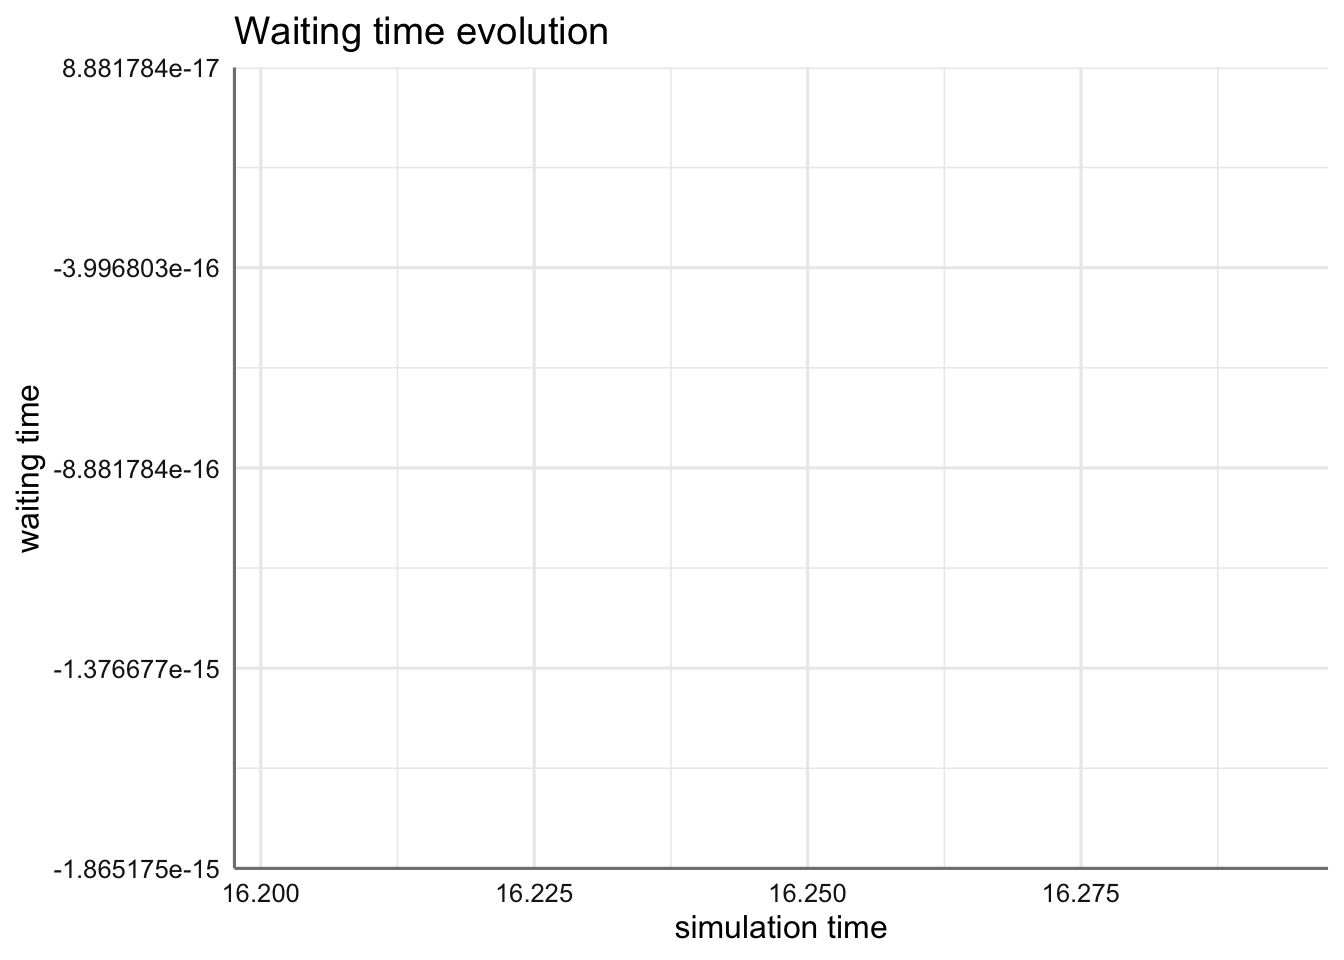
\includegraphics[width=0.95\linewidth]{07-simmer_files/figure-latex/unnamed-chunk-16-1} \end{center}

\begin{Shaded}
\begin{Highlighting}[]
\FunctionTok{plot}\NormalTok{(arrivals, }\AttributeTok{metric=}\StringTok{"activity\_time"}\NormalTok{)}
\end{Highlighting}
\end{Shaded}

\begin{verbatim}
## `geom_smooth()` using method = 'loess' and formula 'y ~ x'
## geom_path: Each group consists of only one observation. Do you need to adjust the group
## aesthetic?
\end{verbatim}

\begin{center}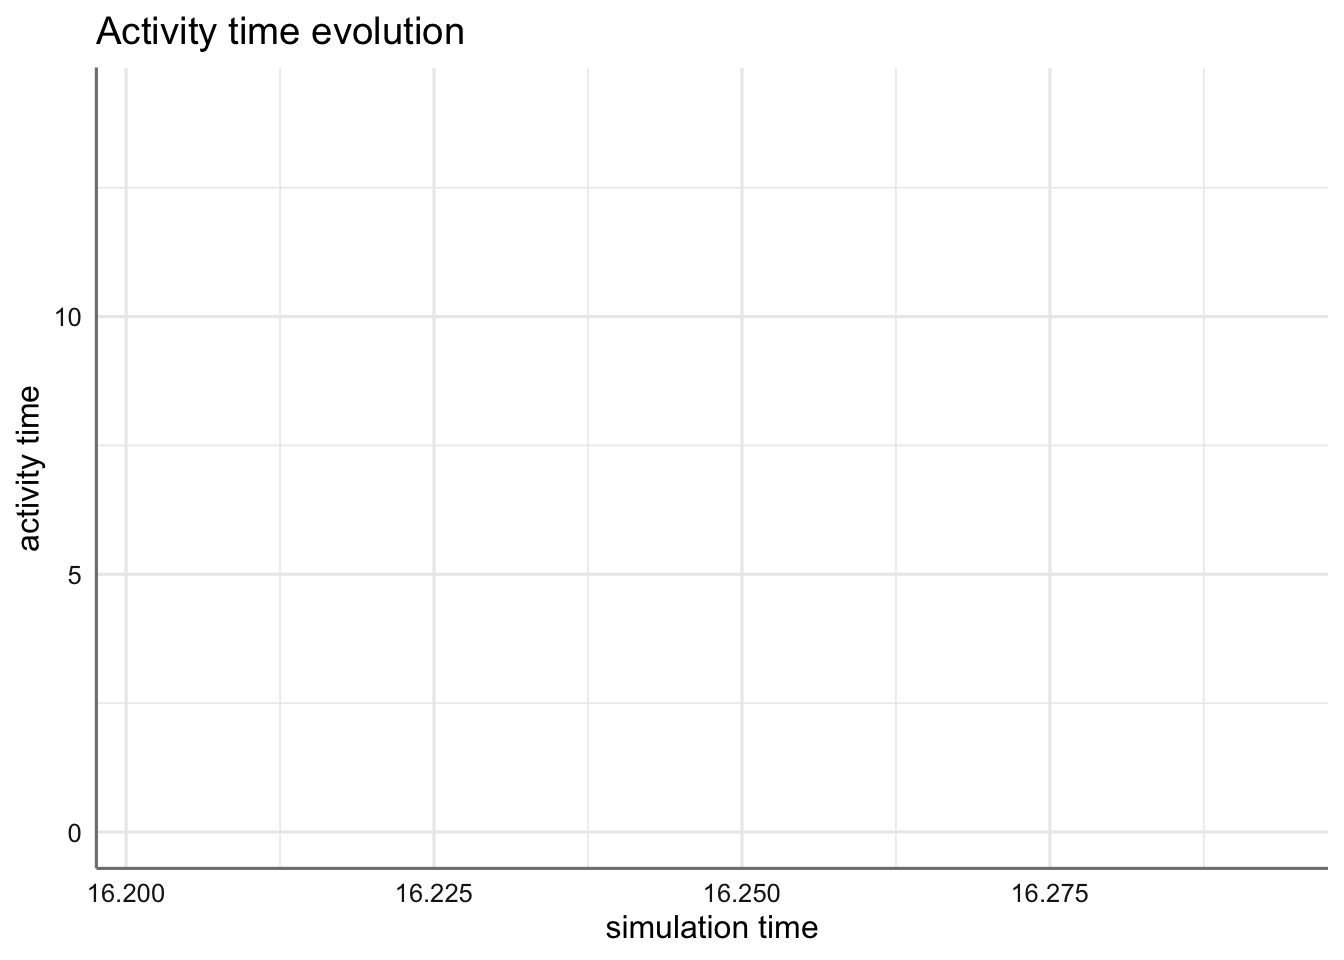
\includegraphics[width=0.95\linewidth]{07-simmer_files/figure-latex/unnamed-chunk-16-2} \end{center}

\begin{Shaded}
\begin{Highlighting}[]
\FunctionTok{plot}\NormalTok{(arrivals, }\AttributeTok{metric=}\StringTok{"flow\_time"}\NormalTok{)}
\end{Highlighting}
\end{Shaded}

\begin{verbatim}
## `geom_smooth()` using method = 'loess' and formula 'y ~ x'
## geom_path: Each group consists of only one observation. Do you need to adjust the group
## aesthetic?
\end{verbatim}

\begin{center}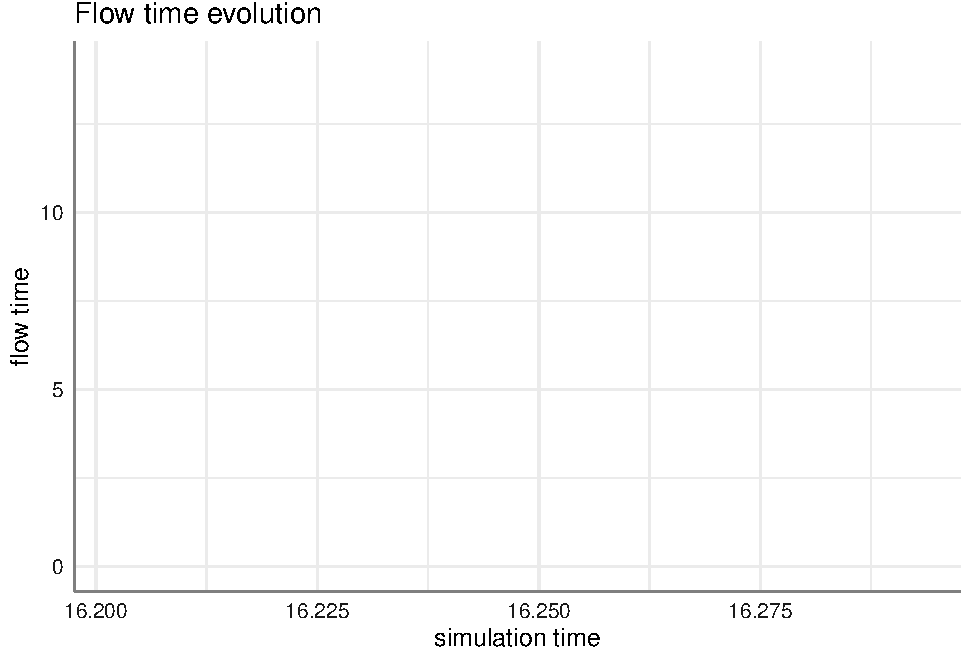
\includegraphics[width=0.95\linewidth]{07-simmer_files/figure-latex/unnamed-chunk-16-3} \end{center}

Para los \textbf{recursos}, tenemos dos métricas de graficado:

\begin{itemize}
\tightlist
\item
  \emph{usage} muestra un gráfico de líneas con el tiempo promedio de uso (acumulado) de cada recurso, replication e item (por defecto queue, server y system, que es la suma de servidor y cola). Si \emph{steps=TRUE}, se pinta un gráfico de escaleras con los valores instantáneos.
\item
  \emph{utilization} muestra un gráfico de barras con el promedio de uso del recurso (tiempo total en uso, dividido por el tiempo total de simulación). Para replicaciones múltiples, la barra representa la mediana y las barras de error los cuartiles. Si se proporciona una única replicación, la barra y la barra de error coinciden.
\end{itemize}

Teniendo en cuenta que \texttt{get\_mon} proporciona objetos data.frame, podemos utilizar cualquier otro tipo de gráfico específico y personalizado con las funciones gráficas habituales de R, y en particular de `ggplot2'.

\begin{Shaded}
\begin{Highlighting}[]
\NormalTok{arrivals}\OtherTok{=}\FunctionTok{get\_mon\_arrivals}\NormalTok{(env\_mon)}
\FunctionTok{ggplot}\NormalTok{(arrivals,}\FunctionTok{aes}\NormalTok{(}\AttributeTok{x=}\NormalTok{activity\_time))}\SpecialCharTok{+}
  \FunctionTok{geom\_histogram}\NormalTok{(}\AttributeTok{fill=}\StringTok{"Skyblue"}\NormalTok{,}\AttributeTok{color=}\StringTok{"blue"}\NormalTok{)}
\end{Highlighting}
\end{Shaded}

\begin{verbatim}
## `stat_bin()` using `bins = 30`. Pick better value with `binwidth`.
\end{verbatim}

\begin{center}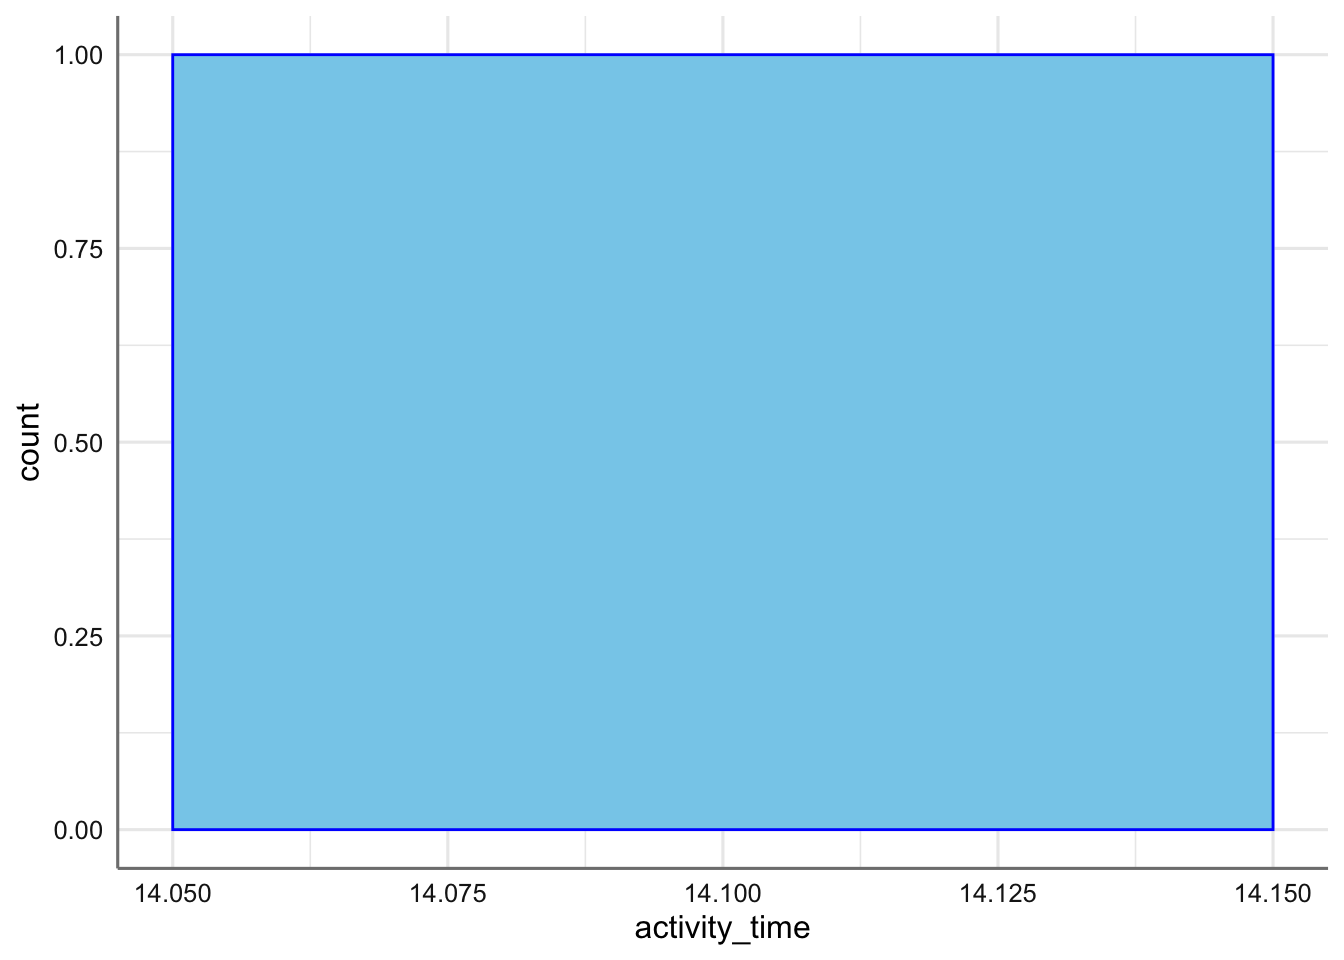
\includegraphics[width=0.95\linewidth]{07-simmer_files/figure-latex/unnamed-chunk-18-1} \end{center}

\hypertarget{acciones}{%
\section{Acciones}\label{acciones}}

Las acciones posibles para definir trayectorias las presentamos a continuación, categorizadas según su funcionalidad:

\begin{longtable}[]{@{}
  >{\raggedright\arraybackslash}p{(\columnwidth - 2\tabcolsep) * \real{0.50}}
  >{\raggedright\arraybackslash}p{(\columnwidth - 2\tabcolsep) * \real{0.50}}@{}}
\toprule
\begin{minipage}[b]{\linewidth}\raggedright
Funciones
\end{minipage} & \begin{minipage}[b]{\linewidth}\raggedright
comandos
\end{minipage} \\
\midrule
\endhead
atributos en llegadas & set\_attribute, get\_attribute, set\_prioritization, get\_prioritization \\
interacción con recursos & seize, release, set\_capacity, set\_queue\_size, set\_seize\_selected, set\_capacity\_selected \\
interacción con fuentes & activate, deactivate, set\_trajectory, set\_source \\
ramificación & branch, clone \\
bucles & rollback \\
ejecución en lotes & batch \\
programación asíncrona & send, wait, trap, untrap \\
renuncias & leave, renege\_in, renege\_if, renege\_abort \\
\bottomrule
\end{longtable}

La Figura 3 muestra con mucha claridad las principales acciones disponibles en \texttt{simmer}.

\begin{figure}

{\centering 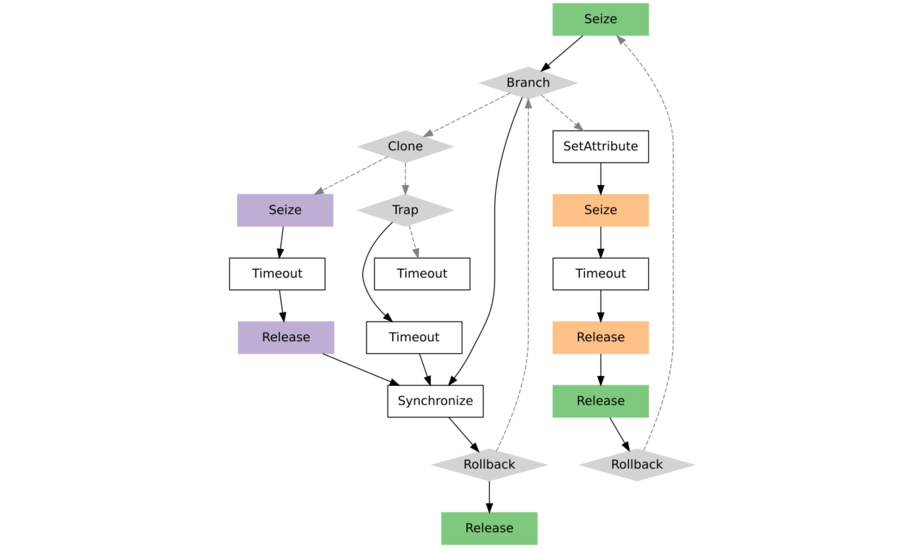
\includegraphics[width=1\linewidth]{images/simmer_trajectory} 

}

\caption{Figura 3. Principales acciones en trayectorias `simmer`. [Fte: IBiDat](https://ibidat.es/portfolio-items/simmer-discrete-event-simulation-for-r/)}\label{fig:simmertray}
\end{figure}

\hypertarget{atributos-en-llegadas}{%
\section{Atributos en llegadas}\label{atributos-en-llegadas}}

Las llegadas pueden almacenar y modificar atributos con el comando \texttt{set\_attribute()}. Los atributos consisten en pares \texttt{(key,value)} que por defecto se asignan por llegada, salvo que se definan globalmente.

proporcionan el nombre (carácter) de la llegada (\emph{key}) que, y el valor que toma (\emph{value}). Estos atributos pueden ser definidos de modo particular a cada llegada, o de modo global. Los atributos \emph{keys} y \emph{values} pueden ser vectores o funciones que devuelvan vectores.

Se especifica con el comando \texttt{set\_attribute}:

\begin{verbatim}
set_attribute(keys, values, mod = c(NA, "+", "*"), init = 0)
\end{verbatim}

que incluye o modifica unos atributos numéricos (\emph{values}) a una llegada o un conjunto de llegadas especificados en el vector \emph{keys}. Las modificaciones se gestionan a través del parámetro \texttt{mod}, que incluye las operaciones más habituales (suma y producto).

Los atributos se pueden recuperar con el comando \texttt{get\_attribute(.env,\ keys)}, siempre que se haya definido previamente un objeto \texttt{simmer} (.env).

Por ejemplo, el siguiente modelo define una entrada en la que se da el valor 60 a peso, luego le suma 1 y visualiza el resultado, que es ``\emph{Mi peso es 61}'':

\begin{Shaded}
\begin{Highlighting}[]
\NormalTok{env}\OtherTok{=}\FunctionTok{simmer}\NormalTok{()}
\NormalTok{traj}\OtherTok{=}\FunctionTok{trajectory}\NormalTok{() }\SpecialCharTok{\%\textgreater{}\%}
  \CommentTok{\# asignamos el atributo numérico a peso}
  \FunctionTok{set\_attribute}\NormalTok{(}\StringTok{"peso"}\NormalTok{,}\DecValTok{60}\NormalTok{) }\SpecialCharTok{\%\textgreater{}\%}
  \CommentTok{\# a continuación lo modificamos}
  \FunctionTok{set\_attribute}\NormalTok{(}\StringTok{"peso"}\NormalTok{,}\DecValTok{1}\NormalTok{,}\AttributeTok{mod=}\StringTok{"+"}\NormalTok{) }\SpecialCharTok{\%\textgreater{}\%}
  \CommentTok{\# y por último lo visualizamos}
  \FunctionTok{log\_}\NormalTok{(}\ControlFlowTok{function}\NormalTok{() }\FunctionTok{paste}\NormalTok{(}\StringTok{"Mi peso es"}\NormalTok{,}\FunctionTok{get\_attribute}\NormalTok{(env,}\StringTok{"peso"}\NormalTok{)))}

\NormalTok{env}\OtherTok{=}\NormalTok{env }\SpecialCharTok{\%\textgreater{}\%}
  \FunctionTok{add\_generator}\NormalTok{(}\StringTok{"peso"}\NormalTok{,traj,}\FunctionTok{at}\NormalTok{(}\DecValTok{1}\NormalTok{)) }\SpecialCharTok{\%\textgreater{}\%}
  \FunctionTok{print}\NormalTok{() }\SpecialCharTok{\%\textgreater{}\%}
  \FunctionTok{run}\NormalTok{()}
\end{Highlighting}
\end{Shaded}

\begin{verbatim}
## simmer environment: anonymous | now: 0 | next: 0
## { Monitor: in memory }
## { Source: peso | monitored: 1 | n_generated: 0 }
## 1: peso0: Mi peso es 61
\end{verbatim}

Las llegadas además, están sujetas a tres posibles valores de prioridad para acceder a los recursos y que son definidas a través del comando \texttt{set\_prioritization},

\begin{verbatim}
set_prioritization(.trj, values, mod = c(NA, "+", "*"))
\end{verbatim}

a través del argumento \texttt{values=c(priority,preemptible,restart)} para todas las llegadas que se crean provenientes de cualquier fuente. El significado de estos argumentos es es siguiente:

\begin{itemize}
\tightlist
\item
  \textbf{prioridad} (\emph{priority}); un valor más alto implica mayor prioridad. El valor por defecto es la mínima prioridad, representada por el 0.
\item
  \textbf{prevención} (\emph{preemptible}); si un recurso es accedido, este valor establece la mínima prioridad de acceso que puede prevenir una llegada, es decir, el acceso al recurso. Si un recurso tiene `prevencion=2' y se produce una llegada con `prioridad=3', la actividad previa se interrumpe y accede al recurso esta llegada, puesto que su orden de prioridad es mayor al de prevención.
\end{itemize}

En cualquier caso, \emph{preemtible} debe ser mayor o igual que \emph{priority}, y por lo tanto sólo las llegadas con prioridad más alta pueden desencadenar una prevención o suspensión inesperada por tener llegadas con mayor prioridad.

\begin{itemize}
\tightlist
\item
  \textbf{reinicio} (\emph{restart}), cuando se ha producido una prevención, indica si al finalizar la actividad con la llegada preferente, el recurso ha de reanudar (TRUE) la actividad previa que hubo de suspender o no (0).
\end{itemize}

El argumento \texttt{mod} permite modificar y cambiar de forma dinámica por llegada. Con \texttt{get\_prioritization(.env)} se obtienen los valores de priorización para acceder a los recursos.

\hypertarget{interacciuxf3n-con-recursos}{%
\section{Interacción con recursos}\label{interacciuxf3n-con-recursos}}

Las dos actividades principales para interaccionar con recursos son \texttt{seize()} -acceso- y \texttt{release()} -salida-. Un recurso o conjunto de recursos (\emph{amount}) entran en funcionamiento con \texttt{seize()} y dejan de funcionar con \texttt{release()}.

\begin{verbatim}
seize(.trj, resource, amount = 1, continue = NULL, post.seize = NULL,reject = NULL)
release(.trj, resource, amount = 1)
\end{verbatim}

La actividad \texttt{seize()} es especial en el sentido de que el resultado o salida depende del estado del recurso. Una llegada, cuando accede a un recurso, puede aprovecharlo con éxito desde el momento en que accede y continuar su camino en la trayectoria, pero también puede ponerse en cola (si el recurso está ocupado) o ser rechazada y despedida de la trayectoria. Para manejar estos casos especiales con total flexibilidad, \texttt{seize()} soporta la especificación de dos sub-trayectorias opcionales:

\begin{itemize}
\tightlist
\item
  \texttt{post.seize}, que es la actividad que sigue despues de un \emph{seize} exitoso, y
\item
  \texttt{reject}, que es la actividad que sigue si la llegada ha sido rechazada.
\end{itemize}

Como en todas las actividades que soportan la definición de sub-trayectorias, hay un parámetro booleano llamado \emph{continue}. Para cada sub-trayectoria, este parámetro controla si las llegadas deberían continuar a la actividad que sigue a \texttt{seize()} en la trayectoria principal después de ejecutar la sub-trayectoria.

Para ejemplificar su uso consideramos un ambulatorio médico al que llegan pacientes. Si al llegar el paciente, el doctor está disponible, es atendido por este durante 5 minutos. Si no está disponible, es rechazado y derivado a consulta de enfermería, donde es atendido siempre 8 minutos, al haber 10 enfermeras disponibles. En ambos casos el paciente se va del ambulatorio al terminar la consulta a la que haya entrado.

\begin{Shaded}
\begin{Highlighting}[]
\NormalTok{env}\OtherTok{=}\FunctionTok{simmer}\NormalTok{()}

\NormalTok{traj}\OtherTok{=}\FunctionTok{trajectory}\NormalTok{() }\SpecialCharTok{\%\textgreater{}\%}
  \FunctionTok{log\_}\NormalTok{(}\ControlFlowTok{function}\NormalTok{() }\FunctionTok{paste}\NormalTok{(}\StringTok{"Llega el "}\NormalTok{,}\FunctionTok{get\_name}\NormalTok{(env))) }\SpecialCharTok{\%\textgreater{}\%}
  \FunctionTok{seize}\NormalTok{(}
    \StringTok{"doctor"}\NormalTok{,}\DecValTok{1}\NormalTok{,}\AttributeTok{continue=}\FunctionTok{c}\NormalTok{(}\ConstantTok{TRUE}\NormalTok{,}\ConstantTok{FALSE}\NormalTok{),}
    \AttributeTok{post.seize=}\FunctionTok{trajectory}\NormalTok{(}\StringTok{"Paciente aceptado"}\NormalTok{) }\SpecialCharTok{\%\textgreater{}\%} 
      \FunctionTok{log\_}\NormalTok{(}\StringTok{"Pasa a consulta con el doctor"}\NormalTok{), }
    \AttributeTok{reject=}\FunctionTok{trajectory}\NormalTok{(}\StringTok{"Paciente rechazado"}\NormalTok{) }\SpecialCharTok{\%\textgreater{}\%} 
      \FunctionTok{log\_}\NormalTok{(}\StringTok{"El doctor está ocupado y es derivado a enfermería"}\NormalTok{) }\SpecialCharTok{\%\textgreater{}\%} 
      \FunctionTok{seize}\NormalTok{(}\StringTok{"nurse"}\NormalTok{,}\DecValTok{1}\NormalTok{) }\SpecialCharTok{\%\textgreater{}\%}
      \FunctionTok{log\_}\NormalTok{(}\StringTok{"Pasa a consulta con la enfermera"}\NormalTok{) }\SpecialCharTok{\%\textgreater{}\%}
      \FunctionTok{timeout}\NormalTok{(}\DecValTok{8}\NormalTok{) }\SpecialCharTok{\%\textgreater{}\%}
      \FunctionTok{release}\NormalTok{(}\StringTok{"nurse"}\NormalTok{,}\DecValTok{1}\NormalTok{) }\SpecialCharTok{\%\textgreater{}\%}
      \FunctionTok{log\_}\NormalTok{(}\ControlFlowTok{function}\NormalTok{() }\FunctionTok{paste}\NormalTok{(}\StringTok{"El"}\NormalTok{,}\FunctionTok{get\_name}\NormalTok{(env), }\StringTok{"sale de enfermería"}\NormalTok{))) }\SpecialCharTok{\%\textgreater{}\%}
  \FunctionTok{timeout}\NormalTok{(}\DecValTok{5}\NormalTok{) }\SpecialCharTok{\%\textgreater{}\%} 
  \FunctionTok{release}\NormalTok{(}\StringTok{"doctor"}\NormalTok{,}\DecValTok{1}\NormalTok{) }\SpecialCharTok{\%\textgreater{}\%} 
  \FunctionTok{log\_}\NormalTok{(}\StringTok{"El doctor ya está libre"}\NormalTok{)}

\NormalTok{env}\OtherTok{=}\NormalTok{env }\SpecialCharTok{\%\textgreater{}\%}
   \FunctionTok{add\_resource}\NormalTok{(}\StringTok{"doctor"}\NormalTok{,}\AttributeTok{capacity=}\DecValTok{1}\NormalTok{,}\AttributeTok{queue\_size=}\DecValTok{0}\NormalTok{) }\SpecialCharTok{\%\textgreater{}\%} 
   \FunctionTok{add\_resource}\NormalTok{(}\StringTok{"nurse"}\NormalTok{,}\AttributeTok{capacity=}\DecValTok{10}\NormalTok{,}\AttributeTok{queue\_size=}\DecValTok{0}\NormalTok{) }\SpecialCharTok{\%\textgreater{}\%}
   \FunctionTok{add\_generator}\NormalTok{(}\StringTok{"paciente"}\NormalTok{,traj,}\FunctionTok{at}\NormalTok{(}\DecValTok{0}\NormalTok{,}\DecValTok{1}\NormalTok{,}\DecValTok{5}\NormalTok{,}\DecValTok{8}\NormalTok{)) }\SpecialCharTok{\%\textgreater{}\%}
   \FunctionTok{run}\NormalTok{()}
\end{Highlighting}
\end{Shaded}

\begin{verbatim}
## 0: paciente0: Llega el  paciente0
## 0: paciente0: Pasa a consulta con el doctor
## 1: paciente1: Llega el  paciente1
## 1: paciente1: El doctor está ocupado y es derivado a enfermería
## 1: paciente1: Pasa a consulta con la enfermera
## 5: paciente0: El doctor ya está libre
## 5: paciente2: Llega el  paciente2
## 5: paciente2: Pasa a consulta con el doctor
## 8: paciente3: Llega el  paciente3
## 8: paciente3: El doctor está ocupado y es derivado a enfermería
## 8: paciente3: Pasa a consulta con la enfermera
## 9: paciente1: El paciente1 sale de enfermería
## 10: paciente2: El doctor ya está libre
## 16: paciente3: El paciente3 sale de enfermería
\end{verbatim}

A la hora de asignar un recurso, podemos hacerlo especificando explícitamente el nombre del recurso (si tenemos varios), o hacerlo de forma dinámica especificando la política a seguir. Esto lo podemos hacer con la actividad \texttt{select()}, a través de los argumentos \emph{resources} y \emph{policy}.

\begin{verbatim}
select(.trj, resources, policy = c("shortest-queue",
  "shortest-queue-available", "round-robin", "round-robin-available",
  "first-available", "random", "random-available"), id = 0)
\end{verbatim}

Hay varias políticas implementadas internamente a las que se puede acceder por su nombre:

\begin{itemize}
\tightlist
\item
  `shortest-queue': se selecciona el recurso con la cola más corta
\item
  `round-robin': se seleccionarán los recursos de una forma cíclica
\item
  `first-available': se selecciona el recurso que queda disponible el primero
\item
  `random': se selecciona un recurso aleatoriamente.
\end{itemize}

El parámetro \emph{resources} también puede ser dinámico e incluso existe la posibilidad de definir políticas específicas. Una vez que un recurso es seleccionado, hay versiones especiales de las actividades mencionadas para interaccionar con los recursos sin especificar su nombre, como son \texttt{seize\_selected()}, \texttt{set\_capacity\_selected()}, etc.

Pongamos como ejemplo una consulta médica con 3 doctores, que atienden a los pacientes de un modo ordenado secuencial conforme llegan a la consulta.

\begin{Shaded}
\begin{Highlighting}[]
\NormalTok{traj }\OtherTok{\textless{}{-}} \FunctionTok{trajectory}\NormalTok{() }\SpecialCharTok{\%\textgreater{}\%}
\NormalTok{  simmer}\SpecialCharTok{::}\FunctionTok{select}\NormalTok{(}\FunctionTok{paste0}\NormalTok{(}\StringTok{"doctor"}\NormalTok{, }\DecValTok{1}\SpecialCharTok{:}\DecValTok{3}\NormalTok{), }\StringTok{"round{-}robin"}\NormalTok{) }\SpecialCharTok{\%\textgreater{}\%}
  \FunctionTok{seize\_selected}\NormalTok{(}\DecValTok{1}\NormalTok{) }\SpecialCharTok{\%\textgreater{}\%}
  \FunctionTok{timeout}\NormalTok{(}\DecValTok{5}\NormalTok{) }\SpecialCharTok{\%\textgreater{}\%}
  \FunctionTok{release\_selected}\NormalTok{(}\DecValTok{1}\NormalTok{)}

\FunctionTok{simmer}\NormalTok{() }\SpecialCharTok{\%\textgreater{}\%}
  \FunctionTok{add\_resource}\NormalTok{(}\StringTok{"doctor1"}\NormalTok{) }\SpecialCharTok{\%\textgreater{}\%}
  \FunctionTok{add\_resource}\NormalTok{(}\StringTok{"doctor2"}\NormalTok{) }\SpecialCharTok{\%\textgreater{}\%}
  \FunctionTok{add\_resource}\NormalTok{(}\StringTok{"doctor3"}\NormalTok{) }\SpecialCharTok{\%\textgreater{}\%}
  \FunctionTok{add\_generator}\NormalTok{(}\StringTok{"patient"}\NormalTok{, traj, }\FunctionTok{at}\NormalTok{(}\DecValTok{0}\NormalTok{, }\DecValTok{1}\NormalTok{, }\DecValTok{2}\NormalTok{)) }\SpecialCharTok{\%\textgreater{}\%}
  \FunctionTok{run}\NormalTok{() }\SpecialCharTok{\%\textgreater{}\%}
  \FunctionTok{get\_mon\_resources}\NormalTok{()}
\end{Highlighting}
\end{Shaded}

\begin{verbatim}
##   resource time server queue capacity queue_size system limit replication
## 1  doctor1    0      1     0        1        Inf      1   Inf           1
## 2  doctor2    1      1     0        1        Inf      1   Inf           1
## 3  doctor3    2      1     0        1        Inf      1   Inf           1
## 4  doctor1    5      0     0        1        Inf      0   Inf           1
## 5  doctor2    6      0     0        1        Inf      0   Inf           1
## 6  doctor3    7      0     0        1        Inf      0   Inf           1
\end{verbatim}

\hypertarget{interacciuxf3n-con-fuentes}{%
\section{Interacción con fuentes}\label{interacciuxf3n-con-fuentes}}

Hay cuatro actividades específicas para modificar las fuentes de llegadas. Una llegada puede activar \texttt{activate()} o desactivar \texttt{deactivate()} una fuente, pero también puede modificar la trayectoria a la que se adhieren las llegadas que aparecen (derivarlas a otras trayectorias), con \texttt{set\_trajectory()}, o especificar una nueva distribución entre-llegadas con \texttt{set\_source()}. Para seleccionar dinámicamente una fuente, el parámetro que especifica el nombre de la fuente en todos estos métodos puede ser dinámico.

\begin{verbatim}
activate(.trj, sources)
deactivate(.trj, sources)
set_trajectory(.trj, sources, trajectory)
set_source(.trj, sources, object)  
\end{verbatim}

En el ejemplo a continuación, una llegada, al acceder a la trayectoria, desactiva la fuente que genera llegadas cada segundo, deja transcurrir 1 segundo y después vuelve a activarla.

\begin{Shaded}
\begin{Highlighting}[]
\NormalTok{traj}\OtherTok{=}\FunctionTok{trajectory}\NormalTok{() }\SpecialCharTok{\%\textgreater{}\%}
  \FunctionTok{deactivate}\NormalTok{(}\StringTok{"dummy"}\NormalTok{) }\SpecialCharTok{\%\textgreater{}\%} 
  \FunctionTok{timeout}\NormalTok{(}\DecValTok{1}\NormalTok{) }\SpecialCharTok{\%\textgreater{}\%} 
  \FunctionTok{activate}\NormalTok{(}\StringTok{"dummy"}\NormalTok{) }

\FunctionTok{simmer}\NormalTok{() }\SpecialCharTok{\%\textgreater{}\%}
  \FunctionTok{add\_generator}\NormalTok{(}\StringTok{"dummy"}\NormalTok{,traj,}\ControlFlowTok{function}\NormalTok{() }\DecValTok{1}\NormalTok{) }\SpecialCharTok{\%\textgreater{}\%} 
  \FunctionTok{run}\NormalTok{(}\DecValTok{10}\NormalTok{) }\SpecialCharTok{\%\textgreater{}\%} 
  \FunctionTok{get\_mon\_arrivals}\NormalTok{()}
\end{Highlighting}
\end{Shaded}

\begin{verbatim}
##     name start_time end_time activity_time finished replication
## 1 dummy0          1        2             1     TRUE           1
## 2 dummy1          3        4             1     TRUE           1
## 3 dummy2          5        6             1     TRUE           1
## 4 dummy3          7        8             1     TRUE           1
\end{verbatim}

En este otro ejemplo se define un simulador que genera llamadas cada 2 segundos y las redirige a la trayectoria `traj2.' Una vez allí, la fuente de llamadas se modifica para que a partir de que la primera llamada finalice (estando 2 segundos en `traj2'), se generen llamadas cada segundo y se redirijan estas a la trayectoria `traj1'.

\begin{Shaded}
\begin{Highlighting}[]
\NormalTok{traj1 }\OtherTok{\textless{}{-}} \FunctionTok{trajectory}\NormalTok{() }\SpecialCharTok{\%\textgreater{}\%}
  \FunctionTok{timeout}\NormalTok{(}\DecValTok{1}\NormalTok{)}

\NormalTok{traj2 }\OtherTok{\textless{}{-}} \FunctionTok{trajectory}\NormalTok{() }\SpecialCharTok{\%\textgreater{}\%}
  \FunctionTok{set\_source}\NormalTok{(}\StringTok{"llamada"}\NormalTok{, }\ControlFlowTok{function}\NormalTok{() }\DecValTok{1}\NormalTok{) }\SpecialCharTok{\%\textgreater{}\%}
  \FunctionTok{set\_trajectory}\NormalTok{(}\StringTok{"llamada"}\NormalTok{, traj1) }\SpecialCharTok{\%\textgreater{}\%}
  \FunctionTok{timeout}\NormalTok{(}\DecValTok{2}\NormalTok{)}

\FunctionTok{simmer}\NormalTok{() }\SpecialCharTok{\%\textgreater{}\%}
  \FunctionTok{add\_generator}\NormalTok{(}\StringTok{"llamada"}\NormalTok{, traj2, }\ControlFlowTok{function}\NormalTok{() }\DecValTok{2}\NormalTok{) }\SpecialCharTok{\%\textgreater{}\%}
  \FunctionTok{run}\NormalTok{(}\DecValTok{6}\NormalTok{) }\SpecialCharTok{\%\textgreater{}\%}
  \FunctionTok{get\_mon\_arrivals}\NormalTok{()}
\end{Highlighting}
\end{Shaded}

\begin{verbatim}
##       name start_time end_time activity_time finished replication
## 1 llamada0          2        4             2     TRUE           1
## 2 llamada1          3        4             1     TRUE           1
## 3 llamada2          4        5             1     TRUE           1
\end{verbatim}

\hypertarget{ramificaciuxf3n}{%
\section{Ramificación}\label{ramificaciuxf3n}}

Una rama (branch) es un punto en una trayectoria en el cual se pueden seguir una o más sub-trayectorias. \texttt{simmer} soporta dos tipos de ramificación:

\begin{itemize}
\item
  La actividad \texttt{branch()} coloca la llegada en una de las sub-trayectorias que dependen de alguna condición evaluada en un parámetro dinámico llamado \emph{option}. Es el equivalente de una condición \emph{if/else}, es decir, si el valor de \emph{option} es `i', entonces se ejecutará la sub-trayectoria `i'.
\item
  Por otro lado, la actividad \texttt{clone()} genera n ramas paralelas (clonadas) y replica la llegada n-1 veces, colocando cada una de ellas en las n sub-trayectorias creadas. \texttt{clone()} es la única actividad de sub-trayectorias que no acepta un parámetro \emph{continue}. Por defecto todos los clones continúan en la trayectoria principal después de esta actividad. Para borrar todos los clones excepto uno, se utiliza la actividad \texttt{synchronize()}.
\end{itemize}

\begin{verbatim}
branch(.trj, option, continue, ...)
clone(.trj, n, ...)
synchronize(.trj, wait = TRUE, mon_all = FALSE)
\end{verbatim}

En el ejemplo a continuación simulamos un juego en el que el jugador lanza una moneda. Si llega durante la primera hora (\emph{now(env)=1}), gana un caramelo y se va, y si no, pierde dos caramelos que ha de regalar a María y a José.

\begin{Shaded}
\begin{Highlighting}[]
\NormalTok{env}\OtherTok{=}\FunctionTok{simmer}\NormalTok{()}

\NormalTok{traj}\OtherTok{=}\FunctionTok{trajectory}\NormalTok{() }\SpecialCharTok{\%\textgreater{}\%}
  \FunctionTok{branch}\NormalTok{(}
    \AttributeTok{option=}\ControlFlowTok{function}\NormalTok{() }\FunctionTok{now}\NormalTok{(env), }\AttributeTok{continue=}\FunctionTok{c}\NormalTok{(}\ConstantTok{FALSE}\NormalTok{,}\ConstantTok{TRUE}\NormalTok{), }\CommentTok{\#si 1 la 1ª trayectoria y se va; si 2 la 2ª trayectoria y sigue}
      \FunctionTok{trajectory}\NormalTok{() }\SpecialCharTok{\%\textgreater{}\%} \FunctionTok{log\_}\NormalTok{(}\ControlFlowTok{function}\NormalTok{() }\FunctionTok{paste}\NormalTok{(}\FunctionTok{get\_name}\NormalTok{(env),}\StringTok{"Ha llegado el instante"}\NormalTok{,}\FunctionTok{now}\NormalTok{(env),}\StringTok{", gana un caramelo y se va."}\NormalTok{)), }
      \FunctionTok{trajectory}\NormalTok{() }\SpecialCharTok{\%\textgreater{}\%} \FunctionTok{log\_}\NormalTok{(}\ControlFlowTok{function}\NormalTok{() }\FunctionTok{paste}\NormalTok{(}\FunctionTok{get\_name}\NormalTok{(env),}\StringTok{"Ha llegado el instante"}\NormalTok{,}\FunctionTok{now}\NormalTok{(env),}\StringTok{"y regala dos caramelos"}\NormalTok{))) }\SpecialCharTok{\%\textgreater{}\%} 
  \FunctionTok{clone}\NormalTok{(}\AttributeTok{n=}\DecValTok{2}\NormalTok{, }
    \FunctionTok{trajectory}\NormalTok{() }\SpecialCharTok{\%\textgreater{}\%} \FunctionTok{log\_}\NormalTok{(}\StringTok{"uno a María"}\NormalTok{), }
    \FunctionTok{trajectory}\NormalTok{() }\SpecialCharTok{\%\textgreater{}\%} \FunctionTok{log\_}\NormalTok{(}\StringTok{"otro a José"}\NormalTok{)) }\SpecialCharTok{\%\textgreater{}\%}  
  \FunctionTok{synchronize}\NormalTok{() }
  
\NormalTok{env }\SpecialCharTok{\%\textgreater{}\%}
  \FunctionTok{add\_generator}\NormalTok{(}\StringTok{"Jugador"}\NormalTok{,traj,}\FunctionTok{at}\NormalTok{(}\DecValTok{1}\NormalTok{,}\DecValTok{2}\NormalTok{)) }\SpecialCharTok{\%\textgreater{}\%}
  \FunctionTok{run}\NormalTok{() }\SpecialCharTok{\%\textgreater{}\%}
\NormalTok{  invisible}
\end{Highlighting}
\end{Shaded}

\begin{verbatim}
## 1: Jugador0: Jugador0 Ha llegado el instante 1 , gana un caramelo y se va.
## 2: Jugador1: Jugador1 Ha llegado el instante 2 y regala dos caramelos
## 2: Jugador1: uno a María
## 2: Jugador1: otro a José
\end{verbatim}

\hypertarget{bucles}{%
\section{Bucles}\label{bucles}}

Hay un comando llamado \texttt{rollback()} útil para moverse hacia atrás en una trayectoria y ejecutar bucles sobre una serie de actividades. Esta actividad provoca que la llegada retroceda un cierto número de actividades \emph{amount} (que pueden ser dinámicas) un cierto número de veces \emph{times}. Si se utiliza una función de chequeo \emph{check}, el parámetro \emph{times} es ignorado y la llegada determina si debe retroceder cada vez que choca con \emph{rollback}.

\begin{verbatim}
rollback(.trj, amount, times = Inf, check = NULL)
\end{verbatim}

En el siguiente ejemplo, un jugador accede a un reto de resistencia en el que ha de levantar pesas y mantenerlas. Por cada 5 minutos que aguante, recibirá una recompensa de 25€. El jugador es capaz de aguantar 30 minutos, pero la máxima recompensa a recibir es de 100€, por lo que se detendrá cuando consiga a esa cantidad.

\begin{Shaded}
\begin{Highlighting}[]
\NormalTok{env }\OtherTok{\textless{}{-}} \FunctionTok{simmer}\NormalTok{()}

\NormalTok{traj }\OtherTok{\textless{}{-}} \FunctionTok{trajectory}\NormalTok{() }\SpecialCharTok{\%\textgreater{}\%}
  \FunctionTok{set\_attribute}\NormalTok{(}\StringTok{"var"}\NormalTok{, }\DecValTok{0}\NormalTok{) }\SpecialCharTok{\%\textgreater{}\%}
  \FunctionTok{log\_}\NormalTok{(}\ControlFlowTok{function}\NormalTok{()}
    \FunctionTok{paste}\NormalTok{(}\StringTok{"Tiempo de resistencia:"}\NormalTok{,}\FunctionTok{now}\NormalTok{(env),}\StringTok{". Ganancia="}\NormalTok{, }\FunctionTok{get\_attribute}\NormalTok{(env, }\StringTok{"var"}\NormalTok{))) }\SpecialCharTok{\%\textgreater{}\%}
  \FunctionTok{set\_attribute}\NormalTok{(}\StringTok{"var"}\NormalTok{, }\DecValTok{25}\NormalTok{, }\AttributeTok{mod=}\StringTok{"+"}\NormalTok{) }\SpecialCharTok{\%\textgreater{}\%}
  \FunctionTok{timeout}\NormalTok{(}\DecValTok{5}\NormalTok{)}\SpecialCharTok{\%\textgreater{}\%}
  \FunctionTok{rollback}\NormalTok{(}\DecValTok{3}\NormalTok{, }\AttributeTok{check=}\ControlFlowTok{function}\NormalTok{() }\FunctionTok{get\_attribute}\NormalTok{(env, }\StringTok{"var"}\NormalTok{) }\SpecialCharTok{\textless{}=} \DecValTok{100}\NormalTok{) }

\NormalTok{env }\SpecialCharTok{\%\textgreater{}\%}
  \FunctionTok{add\_generator}\NormalTok{(}\StringTok{"dummy"}\NormalTok{, traj, }\FunctionTok{at}\NormalTok{(}\DecValTok{0}\NormalTok{)) }\SpecialCharTok{\%\textgreater{}\%}
  \FunctionTok{run}\NormalTok{() }\SpecialCharTok{\%\textgreater{}\%}\NormalTok{ invisible}
\end{Highlighting}
\end{Shaded}

\begin{verbatim}
## 0: dummy0: Tiempo de resistencia: 0 . Ganancia= 0
## 5: dummy0: Tiempo de resistencia: 5 . Ganancia= 25
## 10: dummy0: Tiempo de resistencia: 10 . Ganancia= 50
## 15: dummy0: Tiempo de resistencia: 15 . Ganancia= 75
## 20: dummy0: Tiempo de resistencia: 20 . Ganancia= 100
\end{verbatim}

\hypertarget{ejecuciuxf3n-en-lotes}{%
\section{Ejecución en lotes}\label{ejecuciuxf3n-en-lotes}}

La ejecución en lotes o \emph{batching} consiste en acumular varias llegadas antes de que puedan continuar su camino en la trayectoria de modo unitario. Esto significa, por ejemplo, que si 10 llegadas en un lote intenta acceder a una unidad de cierto recurso, sólo una unidad puede ser asignada, y no las 10. Un lote se puede descomponer con \texttt{separate()}, salvo que se marque como \texttt{permanent=TRUE}.

Por defecto todas las llegadas que acceden a un lote se juntan en él, y esperan hasta que se consigue el número esperado de llegadas \emph{n}. Sin embargo, las llegadas pueden evitar unirse al lote bajo alguna restricción si se proporciona una función booleana opcional, \emph{rule}. También un lote se puede agrupar para acceder a un recurso antes de acumular el tamaño del lote, si se especifica un tiempo límite para acceder con \emph{timeout}. Los lotes se comparten sólo por llegadas que se añaden a la misma trayectoria directamente. Siempre que se necesite un lote compartido globalmente, se ha de especificar un nombre con \emph{name}.

\begin{verbatim}
batch(.trj, n, timeout = 0, permanent = FALSE, name = "", rule = NULL)
separate(.trj)
\end{verbatim}

Un ejemplo de sistema en el que puede tener sentido la ejecución por lotes es la visita guiada a un museo, en la que son precisos 5 visitantes para asignar un guía e iniciar la visita. Si en 10 minutos no se han conseguido los visitantes, se iniciará la visita igualmente con los visitantes disponibles. La visita dura 5 minutos y, puesto que hay un único guía, será preciso esperar a su finalización para empezar la siguiente. Los tiempos entre llegadas provienen de una distribución exponencial de media 5.

\begin{Shaded}
\begin{Highlighting}[]
\FunctionTok{set.seed}\NormalTok{(}\DecValTok{1234}\NormalTok{)}
\NormalTok{env}\OtherTok{=}\FunctionTok{simmer}\NormalTok{()}

\NormalTok{visita}\OtherTok{=}\FunctionTok{trajectory}\NormalTok{() }\SpecialCharTok{\%\textgreater{}\%}
  \FunctionTok{batch}\NormalTok{(}\AttributeTok{n=}\DecValTok{5}\NormalTok{,}\AttributeTok{timeout=}\DecValTok{10}\NormalTok{,}\AttributeTok{name=}\StringTok{"visitaguiada"}\NormalTok{,}\AttributeTok{permanent=}\ConstantTok{FALSE}\NormalTok{) }\SpecialCharTok{\%\textgreater{}\%}
  \FunctionTok{seize}\NormalTok{(}\StringTok{"guia"}\NormalTok{,}\DecValTok{1}\NormalTok{) }\SpecialCharTok{\%\textgreater{}\%}
  \FunctionTok{log\_}\NormalTok{(}\StringTok{"Comienza la visita con el guía"}\NormalTok{) }\SpecialCharTok{\%\textgreater{}\%}
  \FunctionTok{timeout}\NormalTok{(}\DecValTok{5}\NormalTok{) }\SpecialCharTok{\%\textgreater{}\%}
  \FunctionTok{release}\NormalTok{(}\StringTok{"guia"}\NormalTok{,}\DecValTok{1}\NormalTok{) }\SpecialCharTok{\%\textgreater{}\%}
  \FunctionTok{log\_}\NormalTok{(}\StringTok{"Visita terminada"}\NormalTok{) }
  

\NormalTok{env}\OtherTok{=}\NormalTok{env }\SpecialCharTok{\%\textgreater{}\%}
  \FunctionTok{add\_resource}\NormalTok{(}\StringTok{"guia"}\NormalTok{,}\DecValTok{1}\NormalTok{) }\SpecialCharTok{\%\textgreater{}\%}
  \FunctionTok{add\_generator}\NormalTok{(}\StringTok{"visitante"}\NormalTok{, visita,}\ControlFlowTok{function}\NormalTok{() }\FunctionTok{rnorm}\NormalTok{(}\DecValTok{1}\NormalTok{,}\DecValTok{5}\NormalTok{,}\FloatTok{0.5}\NormalTok{)) }\SpecialCharTok{\%\textgreater{}\%}
  \FunctionTok{print}\NormalTok{() }\SpecialCharTok{\%\textgreater{}\%}
  \FunctionTok{run}\NormalTok{(}\AttributeTok{until=}\DecValTok{50}\NormalTok{) }
\end{Highlighting}
\end{Shaded}

\begin{verbatim}
## simmer environment: anonymous | now: 0 | next: 0
## { Monitor: in memory }
## { Resource: guia | monitored: TRUE | server status: 0(1) | queue status: 0(Inf) }
## { Source: visitante | monitored: 1 | n_generated: 0 }
## 14.3965: batch_visitaguiada: Comienza la visita con el guía
## 19.3965: batch_visitaguiada: Visita terminada
## 25.0774: batch_visitaguiada: Comienza la visita con el guía
## 30.0774: batch_visitaguiada: Visita terminada
## 39.3721: batch_visitaguiada: Comienza la visita con el guía
## 44.3721: batch_visitaguiada: Visita terminada
\end{verbatim}

\begin{Shaded}
\begin{Highlighting}[]
\FunctionTok{get\_mon\_arrivals}\NormalTok{(env)}
\end{Highlighting}
\end{Shaded}

\begin{verbatim}
##         name start_time end_time activity_time finished replication
## 1 visitante0   4.396467 19.39647             5     TRUE           1
## 2 visitante1   9.535182 19.39647             5     TRUE           1
## 3 visitante2  15.077402 30.07740             5     TRUE           1
## 4 visitante3  18.904553 30.07740             5     TRUE           1
## 5 visitante4  24.119116 30.07740             5     TRUE           1
## 6 visitante5  29.372144 44.37214             5     TRUE           1
## 7 visitante6  34.084774 44.37214             5     TRUE           1
## 8 visitante7  38.811458 44.37214             5     TRUE           1
\end{verbatim}

\hypertarget{programaciuxf3n-asuxedncrona}{%
\section{Programación asíncrona}\label{programaciuxf3n-asuxedncrona}}

Hay ciertos métodos que permiten eventos asíncronos:

\begin{itemize}
\item
  La actividad \texttt{send()} emite una o más señales (\emph{signals}) a todas las llegadas que se suscriben a ellas. Las señales se pueden desencadenar inmediatamente o después de cierto retraso (\emph{delay}). En ese caso, los dos parámetros, \emph{signals} y \emph{delay}, pueden ser dinámicos.
\item
  Las llegadas pueden bloquearse y esperar con \texttt{wait()} hasta que se recibe cierta señal.
\item
  Con \texttt{trap()} las llegadas pueden suscribirse a señales (\emph{signals}) y (opcionalmente) asignar un manipulador (de señales) \emph{handler}. Si se proporciona el \emph{handler}, la llegada detiene la atividad actual hasta que recibe la señal. Después, la actividad continúa desde el punto de interrupción. Sin embargo, si la llegada está esperando en un recurso de cola, las señales atrapadas se ignoran. Lo mismo ocurre con un lote: todas las señales suscritas antes de entrar a un lote son ignoradas.
\item
  Finalmente la actividad \texttt{untrap()}se puede utilizar para cancelar la suscripción a \emph{signals}.
\end{itemize}

\begin{verbatim}
send(.trj, signals, delay = 0)
wait(.trj)
trap(.trj, signals, handler = NULL, interruptible = TRUE)
untrap(.trj, signals)
\end{verbatim}

Por defecto los manipuladores de señales (\emph{signal handlers}) pueden ser interrumpidos también por otras señales, lo que significa que un manipulador (\emph{handler}) puede permanecer reiniciándose si se están emitiendo suficientes señales. Si se necesita un manipulador que no pueda ser interrumpido, hay que utilizar el parámetro \texttt{interruptible=FALSE} en \texttt{trap()}.

En el ejemplo a continuación, una inteligencia artificial reclama una clave de acceso al usuario para desbloquear un recurso digital y permitirle el acceso. El usuario proporciona la clave de acceso al cabo de 5 segundos. La IA recibe la clave y desbloquea el recurso.

\begin{Shaded}
\begin{Highlighting}[]
\NormalTok{ia.acceso}\OtherTok{=}\FunctionTok{trajectory}\NormalTok{() }\SpecialCharTok{\%\textgreater{}\%}
  \FunctionTok{log\_}\NormalTok{(}\StringTok{"Solicito clave de acceso"}\NormalTok{) }\SpecialCharTok{\%\textgreater{}\%}
  \FunctionTok{trap}\NormalTok{(}\StringTok{"clave"}\NormalTok{) }\SpecialCharTok{\%\textgreater{}\%}
  \FunctionTok{wait}\NormalTok{() }\SpecialCharTok{\%\textgreater{}\%}  
  \FunctionTok{log\_}\NormalTok{(}\StringTok{"Clave recibida y acceso permitido"}\NormalTok{)}

\NormalTok{usuario}\OtherTok{=}\FunctionTok{trajectory}\NormalTok{() }\SpecialCharTok{\%\textgreater{}\%}
  \FunctionTok{log\_}\NormalTok{(}\StringTok{"Clave enviada"}\NormalTok{) }\SpecialCharTok{\%\textgreater{}\%}
  \FunctionTok{send}\NormalTok{(}\StringTok{"clave"}\NormalTok{) }
  
\FunctionTok{simmer}\NormalTok{() }\SpecialCharTok{\%\textgreater{}\%}
  \FunctionTok{add\_generator}\NormalTok{(}\StringTok{"ia.acceso"}\NormalTok{,ia.acceso,}\FunctionTok{at}\NormalTok{(}\DecValTok{0}\NormalTok{)) }\SpecialCharTok{\%\textgreater{}\%}
  \FunctionTok{add\_generator}\NormalTok{(}\StringTok{"usuario"}\NormalTok{,usuario,}\FunctionTok{at}\NormalTok{(}\DecValTok{5}\NormalTok{)) }\SpecialCharTok{\%\textgreater{}\%}
  \FunctionTok{run}\NormalTok{() }\SpecialCharTok{\%\textgreater{}\%}
\NormalTok{  invisible}
\end{Highlighting}
\end{Shaded}

\begin{verbatim}
## 0: ia.acceso0: Solicito clave de acceso
## 5: usuario0: Clave enviada
## 5: ia.acceso0: Clave recibida y acceso permitido
\end{verbatim}

\hypertarget{renuncias}{%
\section{Renuncias}\label{renuncias}}

Además de ser rechazadas cuando tratan de acceder a un recurso, las llegadas pueden dejar una trayectoria en cualquier momento, síncrona o asíncronamente. En principio, renunciar significa que una llegada abandona la trayectoria en un momento dado. La actividad más simple que permite esto es \texttt{leave()}, que inmediatamente desencadena la acción dada alguna probabilidad. Además, \texttt{renege\_in()} y \texttt{renege\_if()} desencadena la renuncia asíncronamente después de algún tiempo \emph{timeout=t} o si se recibe una señal, respectivamente, salvo que la acción sea abortada con \texttt{renege\_abort()}. Los dos métodos \texttt{renege\_in()} y \texttt{renege\_if()} aceptan una subtrayectoria opcional, \emph{out}, que se ejecuta directamente antes de abandonar la trayectoria.

\begin{verbatim}
leave(.trj, prob, out = NULL, keep_seized = TRUE)
renege_in(.trj, t, out = NULL, keep_seized = FALSE)
renege_if(.trj, signal, out = NULL, keep_seized = FALSE)
renege_abort(.trj)
\end{verbatim}

En el ejemplo siguiente los clientes llegan a un banco con un solo empleado, del que se

\begin{Shaded}
\begin{Highlighting}[]
\NormalTok{banco}\OtherTok{=}\FunctionTok{trajectory}\NormalTok{() }\SpecialCharTok{\%\textgreater{}\%}
  \FunctionTok{log\_}\NormalTok{(}\StringTok{"He llegado al banco"}\NormalTok{) }\SpecialCharTok{\%\textgreater{}\%}
  \CommentTok{\# se marcha si no es atendido en 5 minutos}
  \FunctionTok{renege\_in}\NormalTok{(}
    \DecValTok{5}\NormalTok{,}
    \AttributeTok{out=}\FunctionTok{trajectory}\NormalTok{() }\SpecialCharTok{\%\textgreater{}\%}
      \FunctionTok{log\_}\NormalTok{(}\StringTok{"He colmado mi paciencia. Me voy..."}\NormalTok{)) }\SpecialCharTok{\%\textgreater{}\%}
  \FunctionTok{seize}\NormalTok{(}\StringTok{"empleado"}\NormalTok{,}\DecValTok{1}\NormalTok{) }\SpecialCharTok{\%\textgreater{}\%}
  \CommentTok{\# me quedo si soy atendido en 5 minutos}
  \FunctionTok{renege\_abort}\NormalTok{() }\SpecialCharTok{\%\textgreater{}\%}
  \FunctionTok{log\_}\NormalTok{(}\StringTok{"Me están atendiendo"}\NormalTok{) }\SpecialCharTok{\%\textgreater{}\%}
  \FunctionTok{timeout}\NormalTok{(}\DecValTok{10}\NormalTok{) }\SpecialCharTok{\%\textgreater{}\%}
  \FunctionTok{release}\NormalTok{(}\StringTok{"empleado"}\NormalTok{,}\DecValTok{1}\NormalTok{) }\SpecialCharTok{\%\textgreater{}\%}
  \FunctionTok{log\_}\NormalTok{(}\StringTok{"He terminado"}\NormalTok{)}

\FunctionTok{simmer}\NormalTok{() }\SpecialCharTok{\%\textgreater{}\%}
  \FunctionTok{add\_resource}\NormalTok{(}\StringTok{"empleado"}\NormalTok{,}\DecValTok{1}\NormalTok{) }\SpecialCharTok{\%\textgreater{}\%}
  \FunctionTok{add\_generator}\NormalTok{(}\StringTok{"cliente"}\NormalTok{,banco,}\FunctionTok{at}\NormalTok{(}\DecValTok{0}\NormalTok{,}\DecValTok{1}\NormalTok{)) }\SpecialCharTok{\%\textgreater{}\%}
  \FunctionTok{run}\NormalTok{() }\SpecialCharTok{\%\textgreater{}\%}
\NormalTok{  invisible}
\end{Highlighting}
\end{Shaded}

\begin{verbatim}
## 0: cliente0: He llegado al banco
## 0: cliente0: Me están atendiendo
## 1: cliente1: He llegado al banco
## 6: cliente1: He colmado mi paciencia. Me voy...
## 10: cliente0: He terminado
\end{verbatim}

\hypertarget{ejemplos}{%
\section{Ejemplos}\label{ejemplos}}

El concepto de trayectoria desarrollado en \texttt{simmer} da lugar a un modo natural de simular una amplia variedad de problemas relacionados con Cadenas de Markov continuas en el tiempo (CTMC), procesos de nacimiento-muerte y sistemas de colas.

\hypertarget{proceso-industrial}{%
\subsection{Proceso industrial}\label{proceso-industrial}}

Utilizamos la ilustración de un proceso industrial de Pidd (1988), Section 5.3.1, base de la introducción del artículo de Ucar et al (2019), en el que describe de modo completo la simulación del proceso con \texttt{simmer}, y que traducimos y comentamos a continuación.

Consideramos un negocio de trabajos de ingeniería, en la que hay varias máquinas idénticas. Cada máquina es capaz de procesar cualquier trabajo que llegue. Hay un suministro de trabajos sin perspectivas de escasez. Los trabajos se asignan a la primera máquina disponible. El tiempo en completar un trabajo es variable, pero depende de la máquina que se utilice. Las máquinas están a cargo de los operarios, que las revisa y realizan una serie de tareas sobre ellas.

El proceso está pues constituido por dos tipos de recursos:

\begin{itemize}
\tightlist
\item
  máquinas, a las que llegan trabajos (jobs)
\item
  operarios, a los que llegan tareas (tasks)
\end{itemize}

Respecto a cómo ocupan su tiempo de operatividad, distinguimos entre \textbf{estados} y \textbf{actividades}. Estas últimas se refieren a tareas que conllevan cierto tiempo para ser completadas. En la Figura

Las actividades que realizan los operarios son:

\begin{itemize}
\tightlist
\item
  RESET: resetear/reinicializar la máquina, si no muestra desgaste que afecte a su funcionalidad
\item
  RETOOL: reparar la máguina si aprecia algún desgaste que afecta al funcionamiento.
  Después de una reparación (RETOOL) y antes de reiniciar el trabajo, toda máquina ha de ser reinicializada (RESET).
\item
  AWAY: salir un rato para atender sus necesidades personales.
\end{itemize}

La actividad que llevan a cabo las máquinas es la propia realización del trabajo (RUNNING).

Se pueden identificar dos clases de procesos o fuentes de llegadas, que generan:

\begin{itemize}
\tightlist
\item
  los \emph{trabajos de tienda} (shop jobs), que usan las máquinas y las desgastan,
\item
  las \emph{tareas personales} que realizan los operarios que se ausentan (AWAY).
\end{itemize}

En la Figura 1 está representado el flujo de trabajo de este sistema basado en máquinas (a la izquierda) y operarios (a la derecha). En círculos los estados posibles de los recursos y en rectángulos las actividades a completar.

\begin{figure}

{\centering 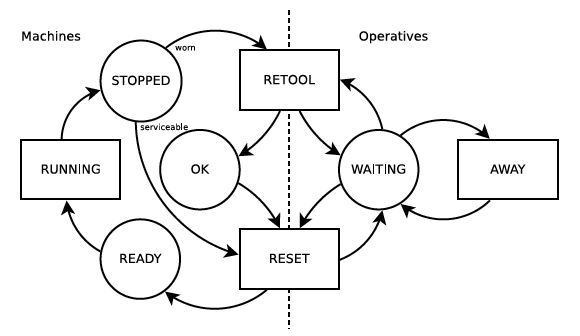
\includegraphics[width=0.8\linewidth]{images/job-cycle} 

}

\caption{Figura 1. Ciclo de trabajo del sistema descrito en Pidd (1988)}\label{fig:job-cycle}
\end{figure}

La forma de simular este sistema con \texttt{simmer} consiste en considerar las máquinas y operarios como recursos y describir como trayectorias los ciclos de los trabajos de tienda y de las tareas personales.

En primer lugar inicializamos un nuevo entorno de simulación y definimos el tiempo de compleción de las diferentes actividades, que vamos a definir según distribuciones exponenciales. Asímismo, se definen los tiempos entre llegadas para los trabajos y las tareas, con NEW\_JOB y NEW\_TASK respectivamente. Consideraremos también una probabilidad 0.2 para que una máquina haya de ser reparada después de hacer un trabajo (CHECK\_WORN).

\begin{Shaded}
\begin{Highlighting}[]
\CommentTok{\# inicializamos una semilla para reproducir siempre las mismas simulaciones}
\FunctionTok{set.seed}\NormalTok{(}\DecValTok{1234}\NormalTok{)}
\CommentTok{\# e inicializamos el entorno de simulación}
\NormalTok{env}\OtherTok{=}\FunctionTok{simmer}\NormalTok{(}\StringTok{"JobShop"}\NormalTok{)}

\CommentTok{\# Definimos cómo se simularán los tiempos de las actividades}
\NormalTok{RUNNING}\OtherTok{=}\ControlFlowTok{function}\NormalTok{() }\FunctionTok{rexp}\NormalTok{(}\DecValTok{1}\NormalTok{,}\DecValTok{1}\NormalTok{)}
\NormalTok{RETOOL}\OtherTok{=} \ControlFlowTok{function}\NormalTok{() }\FunctionTok{rexp}\NormalTok{(}\DecValTok{1}\NormalTok{,}\DecValTok{2}\NormalTok{)}
\NormalTok{RESET}\OtherTok{=} \ControlFlowTok{function}\NormalTok{() }\FunctionTok{rexp}\NormalTok{(}\DecValTok{1}\NormalTok{,}\DecValTok{3}\NormalTok{)}
\NormalTok{AWAY}\OtherTok{=} \ControlFlowTok{function}\NormalTok{() }\FunctionTok{rexp}\NormalTok{(}\DecValTok{1}\NormalTok{,}\DecValTok{1}\NormalTok{)}
\CommentTok{\# chequeo de desgaste y necesidad de reparación}
\NormalTok{CHECK\_WORN}\OtherTok{=}\ControlFlowTok{function}\NormalTok{() }\FunctionTok{runif}\NormalTok{(}\DecValTok{1}\NormalTok{)}\SpecialCharTok{\textless{}}\FloatTok{0.2} \CommentTok{\# da FALSE/TRUE}
\CommentTok{\# y las llegadas de trabajos y tareas personales}
\NormalTok{NEW\_JOB}\OtherTok{=}\ControlFlowTok{function}\NormalTok{() }\FunctionTok{rexp}\NormalTok{(}\DecValTok{1}\NormalTok{,}\DecValTok{5}\NormalTok{)}
\NormalTok{NEW\_TASK}\OtherTok{=}\ControlFlowTok{function}\NormalTok{() }\FunctionTok{rexp}\NormalTok{(}\DecValTok{1}\NormalTok{,}\DecValTok{1}\NormalTok{)}
\end{Highlighting}
\end{Shaded}

La trayectoria de un trabajo (`job') que llega a la tienda, empieza por ocupar (seize) una máquina que está preparada (estado READY). La máquina opera durante cierto tiempo aleatorio (RUNNING) en el que está resolviendo un trabajo. Cuando la máquina finaliza este tiempo, se chequea (CHECK\_WORN) para comprobar si hay que cambiar piezas o no. El chequeo se realiza a través de una ramificación en la que si hay que reparar (con probabilidad 0.2), la máquina accede a la reparación que lleva a cabo el operario durante un tiempo RETOOL; si no, continua con la reinicialización durante un tiempo RESET, también desarrollada por el operario. Finaliza el servicio con la compleción del trabajo del operario y del trabajo de la máquina.

Por otro lado, las tareas personales que realizan los operadores, los mantienen ocupados durante un tiempo AWAY.

\begin{Shaded}
\begin{Highlighting}[]
\NormalTok{job}\OtherTok{=}\FunctionTok{trajectory}\NormalTok{() }\SpecialCharTok{\%\textgreater{}\%}
  \FunctionTok{seize}\NormalTok{(}\StringTok{"máquina"}\NormalTok{) }\SpecialCharTok{\%\textgreater{}\%}
  \FunctionTok{timeout}\NormalTok{(RUNNING) }\SpecialCharTok{\%\textgreater{}\%}
  \FunctionTok{branch}\NormalTok{(}
\NormalTok{    CHECK\_WORN, }\AttributeTok{continue=}\ConstantTok{TRUE}\NormalTok{, }
      \FunctionTok{trajectory}\NormalTok{() }\SpecialCharTok{\%\textgreater{}\%}
        \FunctionTok{seize}\NormalTok{(}\StringTok{"operario"}\NormalTok{) }\SpecialCharTok{\%\textgreater{}\%}
        \FunctionTok{timeout}\NormalTok{(RETOOL) }\SpecialCharTok{\%\textgreater{}\%}
        \FunctionTok{release}\NormalTok{(}\StringTok{"operario"}\NormalTok{)}
\NormalTok{  ) }\SpecialCharTok{\%\textgreater{}\%}
  \FunctionTok{seize}\NormalTok{(}\StringTok{"operario"}\NormalTok{) }\SpecialCharTok{\%\textgreater{}\%}
  \FunctionTok{timeout}\NormalTok{(RESET) }\SpecialCharTok{\%\textgreater{}\%}
  \FunctionTok{release}\NormalTok{(}\StringTok{"operario"}\NormalTok{) }\SpecialCharTok{\%\textgreater{}\%}
  \FunctionTok{release}\NormalTok{(}\StringTok{"máquina"}\NormalTok{)}

\NormalTok{task}\OtherTok{=}\FunctionTok{trajectory}\NormalTok{() }\SpecialCharTok{\%\textgreater{}\%}
  \FunctionTok{seize}\NormalTok{(}\StringTok{"operario"}\NormalTok{) }\SpecialCharTok{\%\textgreater{}\%}
  \FunctionTok{timeout}\NormalTok{(AWAY) }\SpecialCharTok{\%\textgreater{}\%}
  \FunctionTok{release}\NormalTok{(}\StringTok{"operario"}\NormalTok{)}
\end{Highlighting}
\end{Shaded}

Una vez que han sido definidas las trayectorias de los procesos, de las máquinas y de los operarios, dimensionamos el sistema con 10 máquinas idénticas y 5 operarios, y creamos también un generador de trabajos (jobs) y otro de tareas personales (tasks). Dejamos correr el sistema durante 1000 unidades de tiempo.

\begin{Shaded}
\begin{Highlighting}[]
\NormalTok{env }\SpecialCharTok{\%\textgreater{}\%}
  \FunctionTok{add\_resource}\NormalTok{(}\StringTok{"máquina"}\NormalTok{,}\DecValTok{10}\NormalTok{) }\SpecialCharTok{\%\textgreater{}\%}
  \FunctionTok{add\_resource}\NormalTok{(}\StringTok{"operario"}\NormalTok{,}\DecValTok{5}\NormalTok{) }\SpecialCharTok{\%\textgreater{}\%}
  \FunctionTok{add\_generator}\NormalTok{(}\StringTok{"job"}\NormalTok{,job,NEW\_JOB)}\SpecialCharTok{\%\textgreater{}\%}
  \FunctionTok{add\_generator}\NormalTok{(}\StringTok{"task"}\NormalTok{,task,NEW\_TASK) }\SpecialCharTok{\%\textgreater{}\%}
  \FunctionTok{run}\NormalTok{(}\AttributeTok{until=}\DecValTok{1000}\NormalTok{) }\SpecialCharTok{\%\textgreater{}\%}
\NormalTok{  invisible}
\end{Highlighting}
\end{Shaded}

El simulador monitoriza en pantalla todos los cambios de estado y tiempos de vida de todos los procesos, lo que nos permite realizar cualquier tipo de análisis sin demasiado esfuerzo adicional.
Por ejemplo, podríamos extraer el histórico de los estados de los recursos para analizar el número medio de máquinas/operarios utilizados, así como el número de trabajos/tareas esperando ser asignados.

\begin{Shaded}
\begin{Highlighting}[]
\FunctionTok{aggregate}\NormalTok{(}\FunctionTok{cbind}\NormalTok{(server,queue)}\SpecialCharTok{\textasciitilde{}}\NormalTok{resource, }\FunctionTok{get\_mon\_resources}\NormalTok{(env),mean)}
\end{Highlighting}
\end{Shaded}

\begin{verbatim}
##   resource   server     queue
## 1  máquina 7.987438 1.0355590
## 2 operario 3.505732 0.4441298
\end{verbatim}

\hypertarget{sistemas-de-colas}{%
\subsection{Sistemas de colas}\label{sistemas-de-colas}}

Veamos cómo implementar con \texttt{simmer} una cola M/M/1 según el ejemplo mostrado en \href{https://www.r-bloggers.com/2016/04/simulating-queueing-systems-with-simmer/}{FishyOperations, 2016}. Las viñetas de simmer incluyen más ejemplos de sistemas M/M/c/k (\href{https://r-simmer.org/articles/simmer-06-queueing.html}{Ucar, 2020a}), redes de colas y modelos de Markov de tiempo continuo CTMC (\href{https://r-simmer.org/articles/simmer-07-ctmc.html}{Ucar, 2020b}).

En la notación de Kendall (Kendall, 1953), un sistema M/M/1 tiene una distribución de llegadas exponencial con media \(\lambda\), (\textbf{M}/M/1), un único servidor (M/M/\textbf{1}), y un tiempo de servicio exponencial de media \(\mu\), (M/\textbf{M}/1). Por ejemplo, la gente llega a un cajero automático aproximadamente cada \(\lambda\) minutos, espera su turno en la calle y saca dinero durante aproximadamente \(\mu\) minutos. Se definen entonces los parámetros básicos del sistema cuando \(\rho<1\) (para que no se sature el sistema):

\begin{itemize}
\tightlist
\item
  utilización del servidor, \(\rho=\lambda/\mu\)
\item
  promedio de clientes en el sistema (cola y cajero), \(N=\rho/(1-\rho)\)
\item
  tiempo medio en el sistema (ley de Little), \(T=N/\lambda\).
\end{itemize}

Si \(\rho>1\), el sistema es inestable pues hay más llegadas de las que el servidor es capaz de gestionar y la cola crecerá indefinidamente.

La simulación de este sistema con simmer es muy sencilla.

\begin{Shaded}
\begin{Highlighting}[]
\FunctionTok{set.seed}\NormalTok{(}\DecValTok{1234}\NormalTok{)}
\NormalTok{lambda}\OtherTok{=}\DecValTok{2}
\NormalTok{mu}\OtherTok{=}\DecValTok{4}
\NormalTok{rho}\OtherTok{=}\NormalTok{lambda}\SpecialCharTok{/}\NormalTok{mu}

\NormalTok{mm1.cajero}\OtherTok{=}\FunctionTok{trajectory}\NormalTok{() }\SpecialCharTok{\%\textgreater{}\%}
  \FunctionTok{seize}\NormalTok{(}\StringTok{"cajero"}\NormalTok{,}\AttributeTok{amount=}\DecValTok{1}\NormalTok{) }\SpecialCharTok{\%\textgreater{}\%}
  \FunctionTok{timeout}\NormalTok{(}\ControlFlowTok{function}\NormalTok{() }\FunctionTok{rexp}\NormalTok{(}\DecValTok{1}\NormalTok{,mu)) }\SpecialCharTok{\%\textgreater{}\%}
  \FunctionTok{release}\NormalTok{(}\StringTok{"cajero"}\NormalTok{,}\AttributeTok{amount=}\DecValTok{1}\NormalTok{)}

\NormalTok{mm1.env}\OtherTok{=}\FunctionTok{simmer}\NormalTok{() }\SpecialCharTok{\%\textgreater{}\%}
  \FunctionTok{add\_resource}\NormalTok{(}\StringTok{"cajero"}\NormalTok{,}\AttributeTok{capacity=}\DecValTok{1}\NormalTok{,}\AttributeTok{queue\_size=}\ConstantTok{Inf}\NormalTok{) }\SpecialCharTok{\%\textgreater{}\%}
  \FunctionTok{add\_generator}\NormalTok{(}\StringTok{"cliente"}\NormalTok{,mm1.cajero,}\ControlFlowTok{function}\NormalTok{() }\FunctionTok{rexp}\NormalTok{(}\DecValTok{1}\NormalTok{,lambda)) }\SpecialCharTok{\%\textgreater{}\%}
  \FunctionTok{run}\NormalTok{(}\AttributeTok{until=}\DecValTok{2000}\NormalTok{) }
\end{Highlighting}
\end{Shaded}

Después de la especificación de los parámetros (\(\lambda\), \(\mu\)), el primer bloque de código define la trayectoria: cada llegada será asignada al recurso, sacará dinero durante un tiempo variable que responderá a una distribución exponencial con media \(\mu\) y dejará el cajero.

El segundo bloque de código hace una instancia al entorno de simulación, crea el recurso, define el generador de llegadas de clientes y lanza la simulación durante 2000 unidades de tiempo.

A continuación visualizamos los datos simulados de funcionamiento del sistema. En el primer gráfico, la evolución temporal de los recursos: cola y servidor. En el segundo gráfico el tiempo de espera a lo largo del periodo de simulación, y en el tercer gráfico el tiempo de servicio a lo largo del periodo de simulación.

\begin{Shaded}
\begin{Highlighting}[]
\NormalTok{resources}\OtherTok{=}\FunctionTok{get\_mon\_resources}\NormalTok{(mm1.env)}
\NormalTok{arrivals}\OtherTok{=}\FunctionTok{get\_mon\_arrivals}\NormalTok{(mm1.env)}
\FunctionTok{plot}\NormalTok{(resources, }\AttributeTok{metric=}\StringTok{"usage"}\NormalTok{, }\StringTok{"cajero"}\NormalTok{, }\AttributeTok{items =} \FunctionTok{c}\NormalTok{(}\StringTok{"server"}\NormalTok{,}\StringTok{"queue"}\NormalTok{))}
\end{Highlighting}
\end{Shaded}

\begin{center}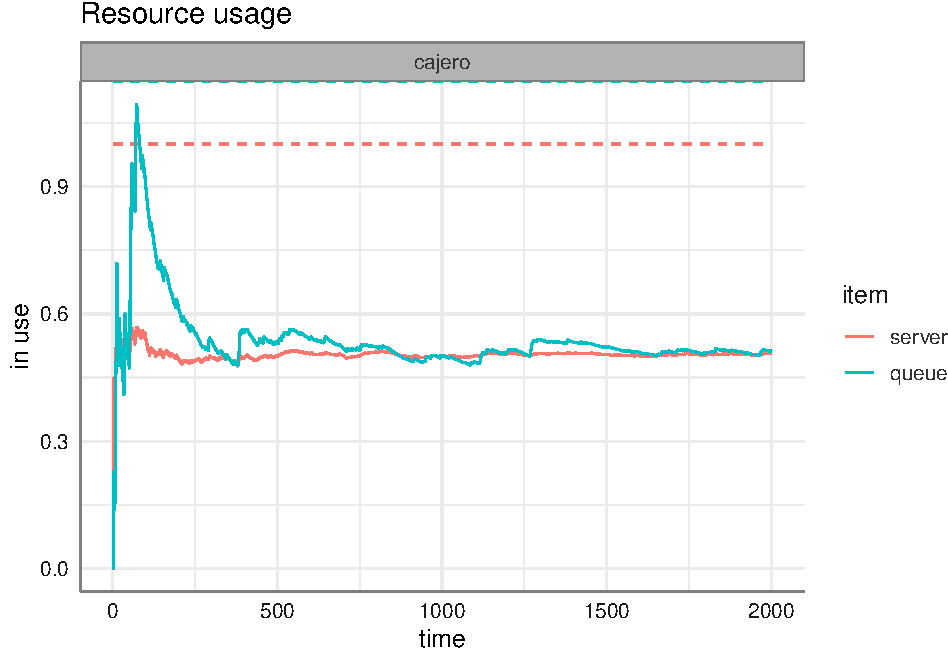
\includegraphics[width=0.95\linewidth]{07-simmer_files/figure-latex/unnamed-chunk-34-1} \end{center}

\begin{Shaded}
\begin{Highlighting}[]
\FunctionTok{plot}\NormalTok{(arrivals, }\AttributeTok{metric=}\StringTok{"waiting\_time"}\NormalTok{)}
\end{Highlighting}
\end{Shaded}

\begin{verbatim}
## `geom_smooth()` using method = 'gam' and formula 'y ~ s(x, bs = "cs")'
\end{verbatim}

\begin{center}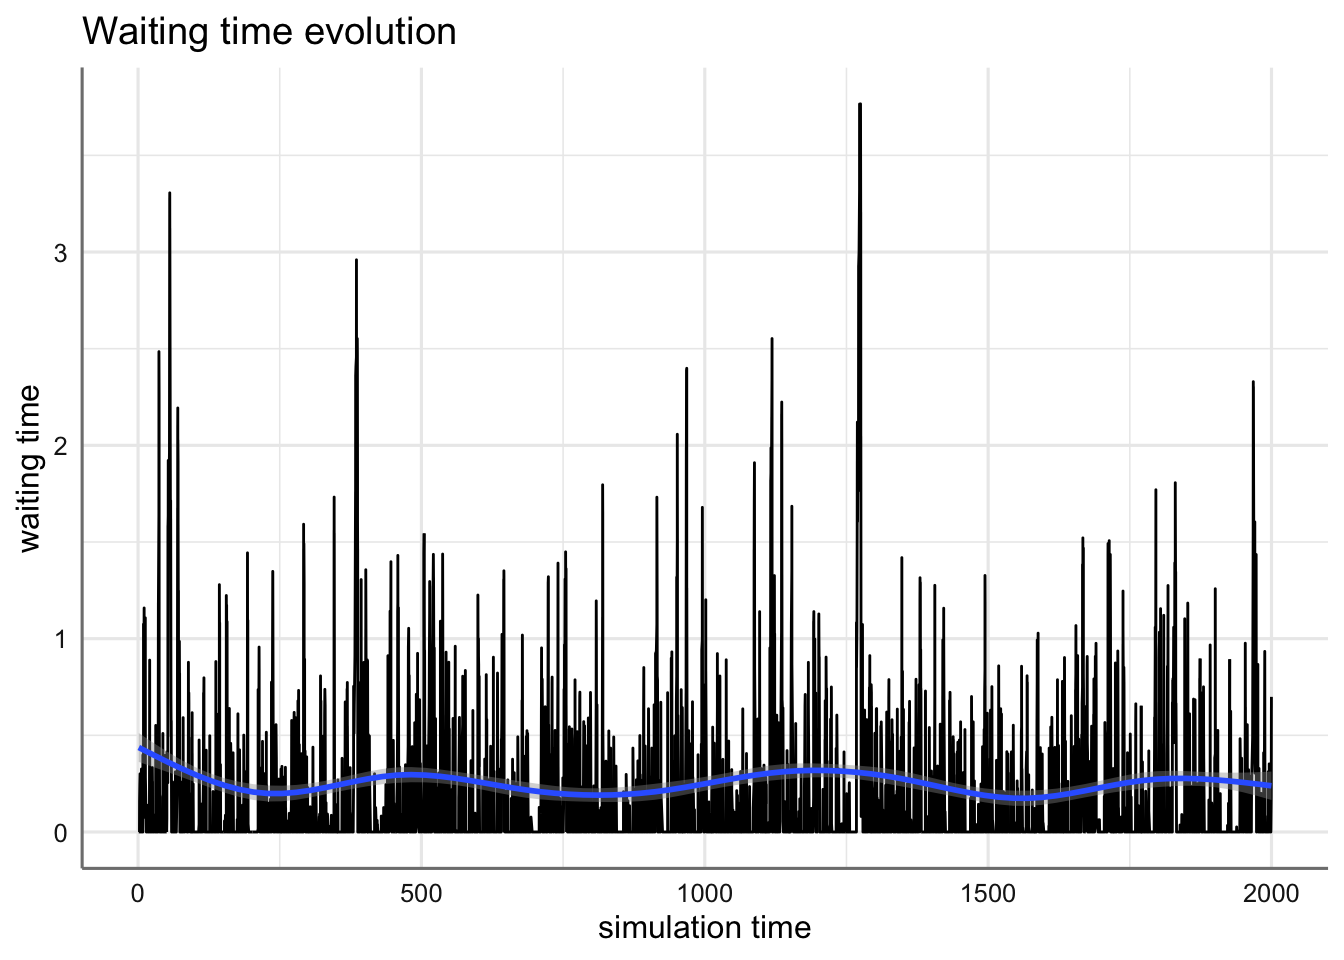
\includegraphics[width=0.95\linewidth]{07-simmer_files/figure-latex/unnamed-chunk-34-2} \end{center}

\begin{Shaded}
\begin{Highlighting}[]
\FunctionTok{plot}\NormalTok{(arrivals, }\AttributeTok{metric=}\StringTok{"activity\_time"}\NormalTok{)}
\end{Highlighting}
\end{Shaded}

\begin{verbatim}
## `geom_smooth()` using method = 'gam' and formula 'y ~ s(x, bs = "cs")'
\end{verbatim}

\begin{center}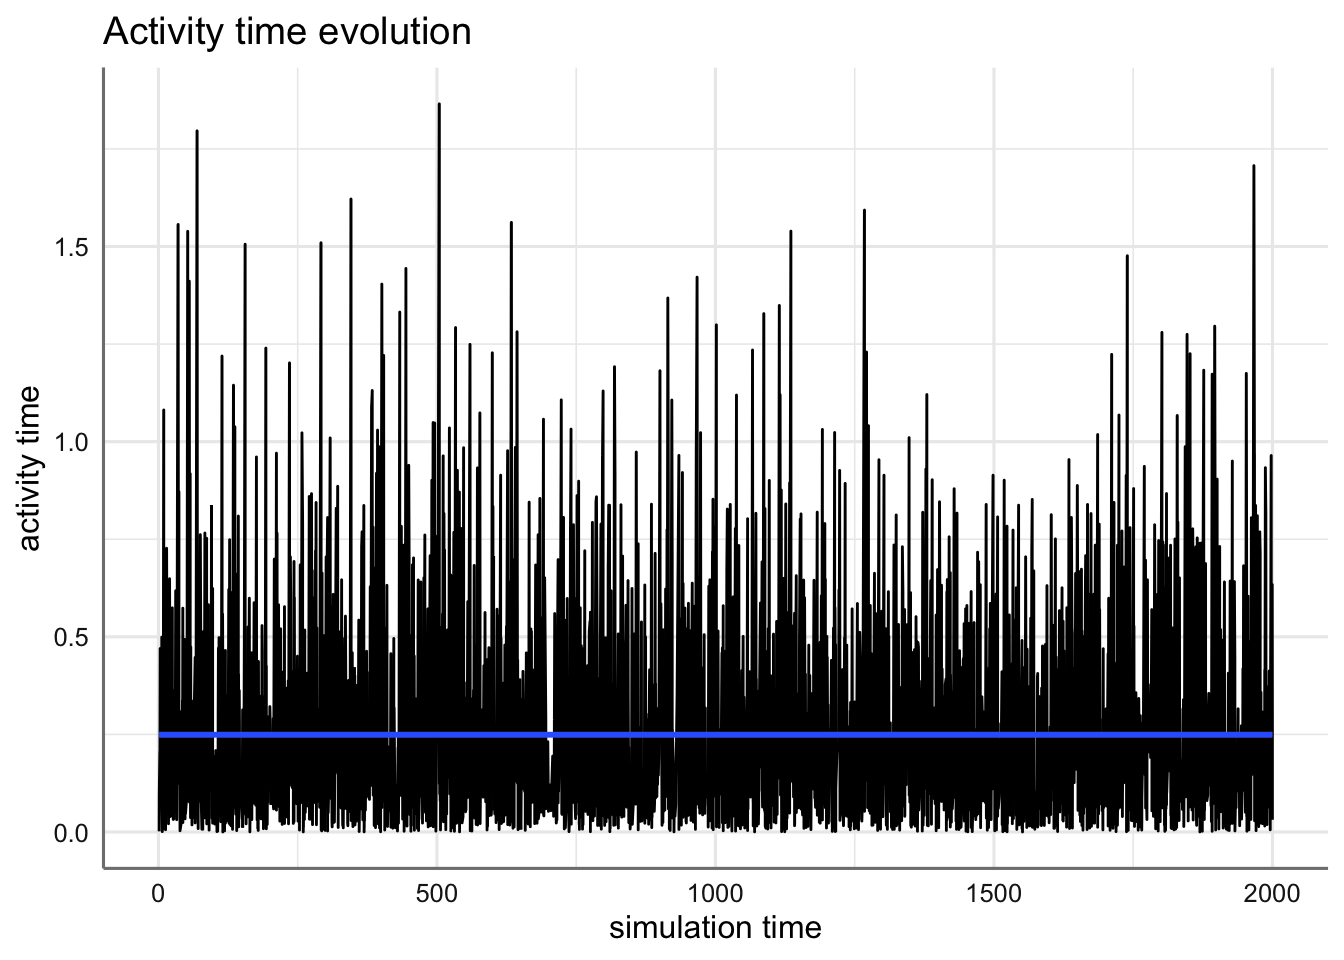
\includegraphics[width=0.95\linewidth]{07-simmer_files/figure-latex/unnamed-chunk-34-3} \end{center}

Si queremos inferir sobre el funcionamiento del sistema a largo plazo, necesitaremos muestras, obtenidas de varias réplicas. La replicación es recomendable llevarla a cabo con la librería \emph{parallel}, que permite lanzar en paralelo varias réplicas simultáneas.

\begin{Shaded}
\begin{Highlighting}[]
\CommentTok{\#library(parallel)}
\NormalTok{mm1.envs}\OtherTok{=}\FunctionTok{mclapply}\NormalTok{(}\DecValTok{1}\SpecialCharTok{:}\DecValTok{100}\NormalTok{,}\ControlFlowTok{function}\NormalTok{(i) \{ }
     \FunctionTok{simmer}\NormalTok{() }\SpecialCharTok{\%\textgreater{}\%}
        \FunctionTok{add\_resource}\NormalTok{(}\StringTok{"cajero"}\NormalTok{,}\AttributeTok{capacity=}\DecValTok{1}\NormalTok{,}\AttributeTok{queue\_size=}\ConstantTok{Inf}\NormalTok{) }\SpecialCharTok{\%\textgreater{}\%}
        \FunctionTok{add\_generator}\NormalTok{(}\StringTok{"cliente"}\NormalTok{,mm1.cajero,}\ControlFlowTok{function}\NormalTok{() }\FunctionTok{rexp}\NormalTok{(}\DecValTok{100}\NormalTok{,lambda)) }\SpecialCharTok{\%\textgreater{}\%}
        \FunctionTok{run}\NormalTok{(}\AttributeTok{until=}\DecValTok{1000}\SpecialCharTok{/}\NormalTok{lambda) }\SpecialCharTok{\%\textgreater{}\%}
       \FunctionTok{wrap}\NormalTok{()}
\NormalTok{     \}, }\AttributeTok{mc.set.seed=}\ConstantTok{FALSE}\NormalTok{)}
\end{Highlighting}
\end{Shaded}

Al recuperar las llegadas con \texttt{get\_mon\_arrivals}, obtenemos un data.frame con todas las llegadas, el instante de llegada (\emph{start\_time}) y salida (\emph{end\_time}), así como el tiempo en servicio -sin contar espera- (\emph{activity\_time}), un indicador de si ha finalizado la actividad (\emph{finished}) y un índice de replicación (\emph{replication}).

\begin{Shaded}
\begin{Highlighting}[]
\NormalTok{mm1.arrivals}\OtherTok{=}\FunctionTok{get\_mon\_arrivals}\NormalTok{(mm1.envs) }
\FunctionTok{head}\NormalTok{(mm1.arrivals)}
\end{Highlighting}
\end{Shaded}

\begin{verbatim}
##       name start_time  end_time activity_time finished replication
## 1 cliente0  0.3373840 0.3988817    0.06149772     TRUE           1
## 2 cliente1  0.8873295 1.0936262    0.20629668     TRUE           1
## 3 cliente2  1.0175261 1.3095587    0.21593254     TRUE           1
## 4 cliente3  1.2768201 1.7538044    0.44424568     TRUE           1
## 5 cliente4  1.6875986 1.9712527    0.21744829     TRUE           1
## 6 cliente5  1.8805297 2.1871458    0.21589316     TRUE           1
\end{verbatim}

Con varias réplicas podríamos, por ejemplo, calcular el tiempo medio en el sistema (\emph{end\_time-start\_time}), y con todas las medias, testar si el tiempo medio es superior o inferior a cualquier valor que marquemos, utilizando en este caso un test t-Student:

\begin{Shaded}
\begin{Highlighting}[]
\NormalTok{mm1.data}\OtherTok{=}\FunctionTok{get\_mon\_arrivals}\NormalTok{(mm1.envs) }\SpecialCharTok{\%\textgreater{}\%}
  \FunctionTok{group\_by}\NormalTok{(replication) }\SpecialCharTok{\%\textgreater{}\%}
  \FunctionTok{summarise}\NormalTok{(}\AttributeTok{m=}\FunctionTok{mean}\NormalTok{(end\_time}\SpecialCharTok{{-}}\NormalTok{start\_time))}
\FunctionTok{ggplot}\NormalTok{(mm1.data,}\FunctionTok{aes}\NormalTok{(}\AttributeTok{x=}\NormalTok{replication,}\AttributeTok{y=}\NormalTok{m))}\SpecialCharTok{+}
  \FunctionTok{geom\_point}\NormalTok{()}\SpecialCharTok{+}
  \FunctionTok{geom\_line}\NormalTok{()}
\end{Highlighting}
\end{Shaded}

\begin{center}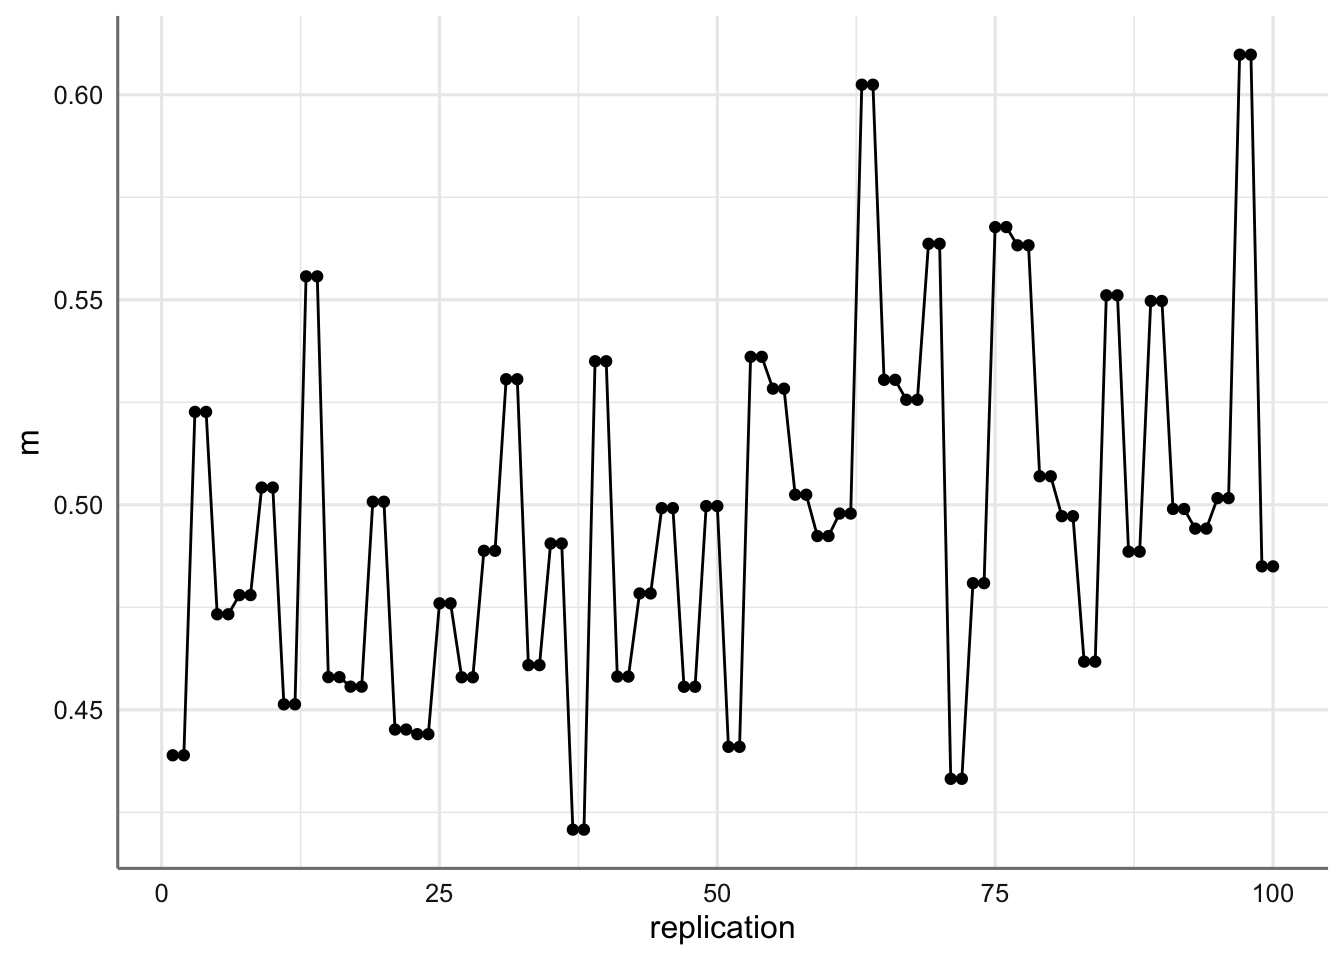
\includegraphics[width=0.95\linewidth]{07-simmer_files/figure-latex/unnamed-chunk-37-1} \end{center}

\begin{Shaded}
\begin{Highlighting}[]
\FunctionTok{t.test}\NormalTok{(mm1.data}\SpecialCharTok{$}\NormalTok{m,}\AttributeTok{mu=}\FloatTok{0.5}\NormalTok{,}\AttributeTok{alternative =}\StringTok{"greater"}\NormalTok{)}
\end{Highlighting}
\end{Shaded}

\begin{verbatim}
## 
##  One Sample t-test
## 
## data:  mm1.data$m
## t = -0.51444, df = 99, p-value = 0.696
## alternative hypothesis: true mean is greater than 0.5
## 95 percent confidence interval:
##  0.4906473       Inf
## sample estimates:
## mean of x 
## 0.4977877
\end{verbatim}

O estudiar la utilización de los recursos,

\begin{Shaded}
\begin{Highlighting}[]
\NormalTok{mm1.resources}\OtherTok{=}\FunctionTok{get\_mon\_resources}\NormalTok{(mm1.envs)}
\FunctionTok{plot}\NormalTok{(mm1.resources, }\AttributeTok{metric=}\StringTok{"utilization"}\NormalTok{)}
\end{Highlighting}
\end{Shaded}

\begin{center}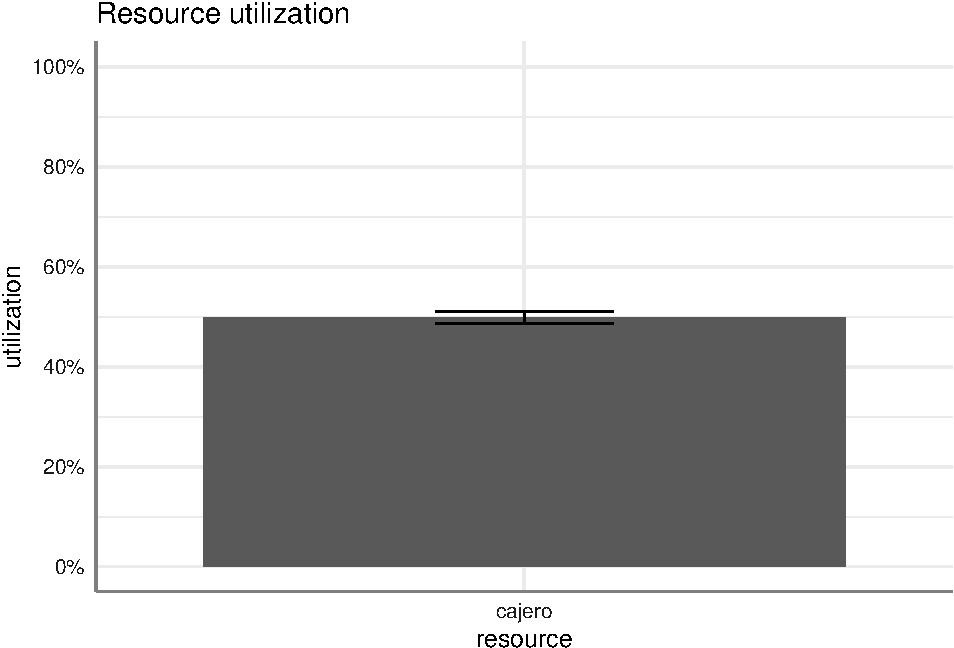
\includegraphics[width=0.95\linewidth]{07-simmer_files/figure-latex/unnamed-chunk-38-1} \end{center}

O incluso testar si el tamaño de la cola (o de sujetos en el sistema) ha sido cero (o cualquier otro valor),

\begin{Shaded}
\begin{Highlighting}[]
\NormalTok{mm1.data}\OtherTok{=}\FunctionTok{get\_mon\_resources}\NormalTok{(mm1.envs) }\SpecialCharTok{\%\textgreater{}\%}
  \FunctionTok{group\_by}\NormalTok{(replication) }\SpecialCharTok{\%\textgreater{}\%}
  \FunctionTok{summarise}\NormalTok{(}\AttributeTok{n.cola=}\FunctionTok{mean}\NormalTok{(queue),}\AttributeTok{n.sistema=}\FunctionTok{mean}\NormalTok{(system))}
\FunctionTok{ggplot}\NormalTok{(mm1.data,}\FunctionTok{aes}\NormalTok{(}\AttributeTok{x=}\NormalTok{replication,}\AttributeTok{y=}\NormalTok{n.cola))}\SpecialCharTok{+}
  \FunctionTok{geom\_point}\NormalTok{()}\SpecialCharTok{+}
  \FunctionTok{geom\_line}\NormalTok{()}\SpecialCharTok{+}
  \FunctionTok{geom\_point}\NormalTok{(}\FunctionTok{aes}\NormalTok{(}\AttributeTok{y=}\NormalTok{n.sistema),}\AttributeTok{color=}\StringTok{"blue"}\NormalTok{)}\SpecialCharTok{+}
  \FunctionTok{geom\_line}\NormalTok{(}\FunctionTok{aes}\NormalTok{(}\AttributeTok{y=}\NormalTok{n.sistema),}\AttributeTok{color=}\StringTok{"blue"}\NormalTok{)}\SpecialCharTok{+}
  \FunctionTok{labs}\NormalTok{(}\AttributeTok{x=}\StringTok{"Replicación"}\NormalTok{,}\AttributeTok{y=}\StringTok{"Usuarios"}\NormalTok{,}\AttributeTok{caption=}\StringTok{"Figura x. Usuarios en cola (negro) y en el sistema (azul)."}\NormalTok{)}
\end{Highlighting}
\end{Shaded}

\begin{center}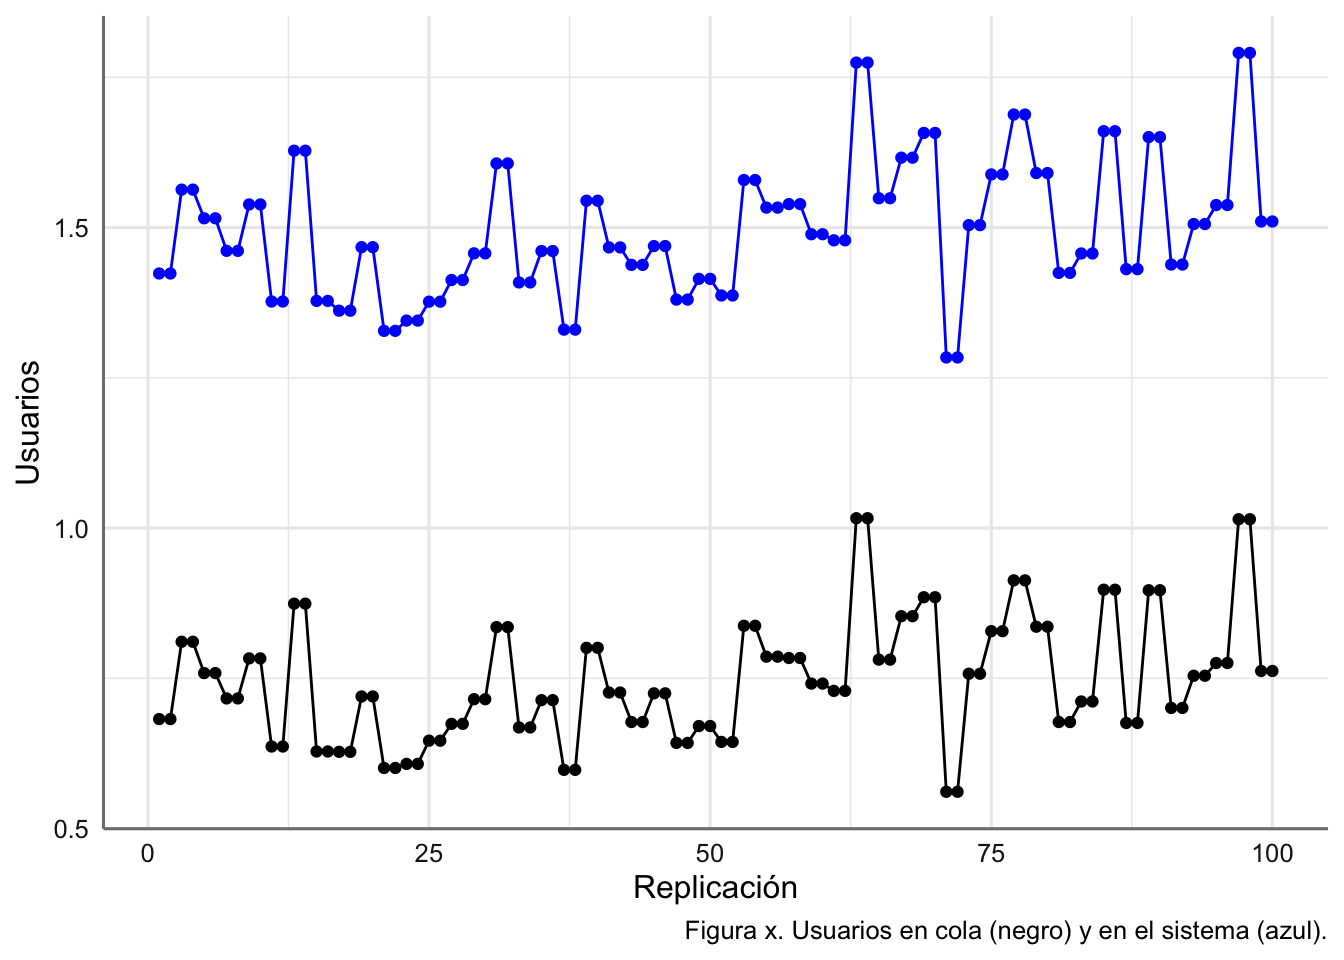
\includegraphics[width=0.95\linewidth]{07-simmer_files/figure-latex/unnamed-chunk-39-1} \end{center}

\begin{Shaded}
\begin{Highlighting}[]
\FunctionTok{t.test}\NormalTok{(mm1.data}\SpecialCharTok{$}\NormalTok{n.cola,}\AttributeTok{mu=}\DecValTok{0}\NormalTok{,}\AttributeTok{alternative =} \StringTok{"greater"}\NormalTok{)}
\end{Highlighting}
\end{Shaded}

\begin{verbatim}
## 
##  One Sample t-test
## 
## data:  mm1.data$n.cola
## t = 72.742, df = 99, p-value < 2.2e-16
## alternative hypothesis: true mean is greater than 0
## 95 percent confidence interval:
##  0.7300316       Inf
## sample estimates:
## mean of x 
## 0.7470844
\end{verbatim}

\begin{Shaded}
\begin{Highlighting}[]
\FunctionTok{t.test}\NormalTok{(mm1.data}\SpecialCharTok{$}\NormalTok{n.sistema,}\AttributeTok{mu=}\DecValTok{1}\NormalTok{,}\AttributeTok{alternative =} \StringTok{"greater"}\NormalTok{)}
\end{Highlighting}
\end{Shaded}

\begin{verbatim}
## 
##  One Sample t-test
## 
## data:  mm1.data$n.sistema
## t = 44.214, df = 99, p-value < 2.2e-16
## alternative hypothesis: true mean is greater than 1
## 95 percent confidence interval:
##  1.477677      Inf
## sample estimates:
## mean of x 
##  1.496315
\end{verbatim}

\hypertarget{gasolinera}{%
\subsection{Gasolinera}\label{gasolinera}}

El ejemplo de la gasolinera es ofrecido en \href{https://r-simmer.org/articles/simmer-07-ctmc.html}{Ucar (2020b)} como una ejemplificación de un proceso de cadena de markov continuo en el tiempo.
Una gasolinera tiene un único surtidor y no dispone de espacio de espera para los vehículos (si un vehículo llega mientras otro está utilizando el surtidor, ha de marcharse). Los vehículos llegan a la gasolinera según un proceso de Poisson de razón \(\lambda=3/20\) vehículos por minuto. De los vehículos que llegan, el 75\% son coches y el resto motocicletas. El tiempo de carga de combustible responde a una distribución exponencial con media 8 minutos para los coches y 3 para las motocicletas.

Recordemos que un proceso de Poisson de parámetro \(\lambda\) implica una distribución de Poisson \(Po(\lambda t)\) para el número de usuarios del sistema transcurrido un tiempo \(t\) y una distribución \(Exp(\lambda)\) para los tiempos entre llegadas de los usuarios.

Puesto que se trata de un proceso continuo en el tiempo, definimos una función que ejecuta el proceso hasta un instante \(t\). El único surtidor de la gasolinera constituye el recurso del proceso, con capacidad 1 y tamaño de la cola 0, y las llegadas de vehículos se generan según una distribución \(Exp(\lambda)\). Al producirse una llegada, se deriva al surtidor, especificando \texttt{amount=1} para provocar que si está ocupado, el vehículo se marcha (es rechazado). Puesto que el tiempo de recarga de combustible depende de si el vehículo es coche o motocicleta, y estos llegan en una proporción 3 a 1 (75\% coches-25\% motos), el tiempo de permanencia en el surtidor especificado con \texttt{timeout} se genera con probabilidad 0.75 con una \(Exp(1/8)\) y con probabilidad 0.25 con una \(Exp(1/3)\). Transcurrido ese tiempo, el vehículo abandona el sistema.

\begin{Shaded}
\begin{Highlighting}[]
\NormalTok{ recarga}\OtherTok{\textless{}{-}} \ControlFlowTok{function}\NormalTok{(t) \{}
\NormalTok{  vehiculo }\OtherTok{\textless{}{-}} \FunctionTok{trajectory}\NormalTok{() }\SpecialCharTok{\%\textgreater{}\%}
    \FunctionTok{seize}\NormalTok{(}\StringTok{"surtidor"}\NormalTok{, }\AttributeTok{amount=}\DecValTok{1}\NormalTok{) }\SpecialCharTok{\%\textgreater{}\%}
    \FunctionTok{timeout}\NormalTok{(}\ControlFlowTok{function}\NormalTok{() \{}
      \ControlFlowTok{if}\NormalTok{ (}\FunctionTok{runif}\NormalTok{(}\DecValTok{1}\NormalTok{) }\SpecialCharTok{\textless{}}\NormalTok{ p) }\FunctionTok{rexp}\NormalTok{(}\DecValTok{1}\NormalTok{, mu[}\DecValTok{1}\NormalTok{])  }\CommentTok{\# coche}
      \ControlFlowTok{else} \FunctionTok{rexp}\NormalTok{(}\DecValTok{1}\NormalTok{, mu[}\DecValTok{2}\NormalTok{])               }\CommentTok{\# moto}
\NormalTok{    \}) }\SpecialCharTok{\%\textgreater{}\%}
    \FunctionTok{release}\NormalTok{(}\StringTok{"surtidor"}\NormalTok{, }\AttributeTok{amount=}\DecValTok{1}\NormalTok{)}

\FunctionTok{simmer}\NormalTok{() }\SpecialCharTok{\%\textgreater{}\%}
    \FunctionTok{add\_resource}\NormalTok{(}\StringTok{"surtidor"}\NormalTok{, }\AttributeTok{capacity=}\DecValTok{1}\NormalTok{, }\AttributeTok{queue\_size=}\DecValTok{0}\NormalTok{) }\SpecialCharTok{\%\textgreater{}\%}
    \FunctionTok{add\_generator}\NormalTok{(}\StringTok{"vehiculo"}\NormalTok{, vehiculo, }\ControlFlowTok{function}\NormalTok{() }\FunctionTok{rexp}\NormalTok{(}\DecValTok{1}\NormalTok{, lambda)) }\SpecialCharTok{\%\textgreater{}\%}
    \FunctionTok{run}\NormalTok{(}\AttributeTok{until=}\NormalTok{t)}
\NormalTok{ \}}
\end{Highlighting}
\end{Shaded}

Definiendo los valores de los parámetros, hacemos correr el sistema hasta el instante \(t=5000\), y visualizamos llegadas y recurso.

\begin{Shaded}
\begin{Highlighting}[]
\NormalTok{t}\OtherTok{=}\DecValTok{5000}
\NormalTok{lambda}\OtherTok{=}\DecValTok{3}\SpecialCharTok{/}\DecValTok{20}
\NormalTok{mu}\OtherTok{=}\FunctionTok{c}\NormalTok{(}\DecValTok{1}\SpecialCharTok{/}\DecValTok{8}\NormalTok{,}\DecValTok{1}\SpecialCharTok{/}\DecValTok{3}\NormalTok{)}
\NormalTok{p}\OtherTok{=}\FloatTok{0.75}
 
\NormalTok{gasolinera}\OtherTok{=}\FunctionTok{recarga}\NormalTok{(t) }
\NormalTok{llegadas}\OtherTok{=}\FunctionTok{get\_mon\_arrivals}\NormalTok{(gasolinera)}
\NormalTok{surtidor}\OtherTok{=}\FunctionTok{get\_mon\_resources}\NormalTok{(gasolinera)}
\FunctionTok{plot}\NormalTok{(llegadas, }\AttributeTok{metric=}\StringTok{"activity\_time"}\NormalTok{)}
\end{Highlighting}
\end{Shaded}

\begin{verbatim}
## `geom_smooth()` using method = 'loess' and formula 'y ~ x'
\end{verbatim}

\begin{center}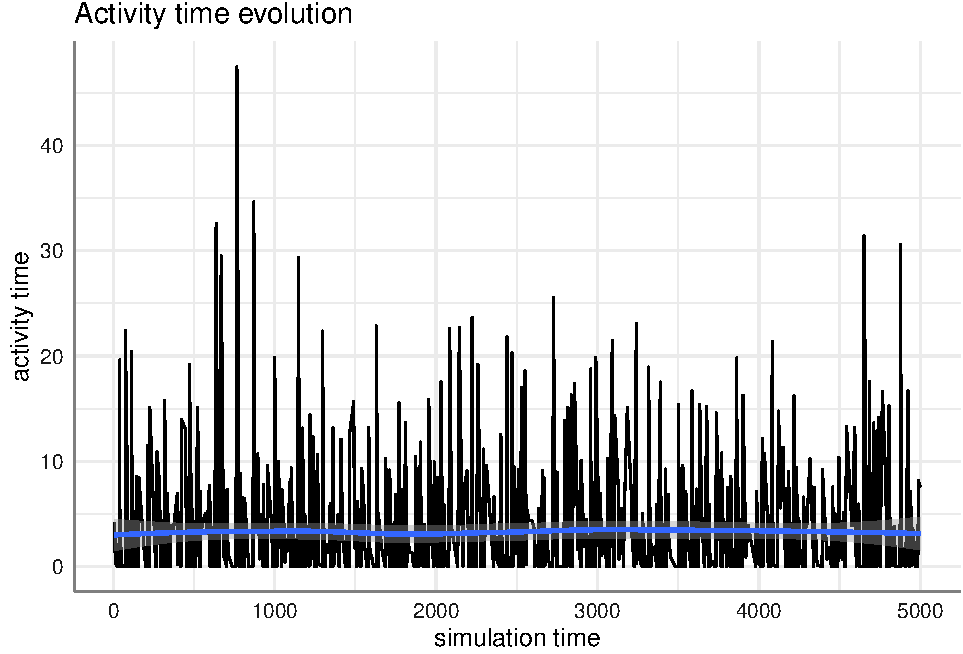
\includegraphics[width=0.95\linewidth]{07-simmer_files/figure-latex/unnamed-chunk-41-1} \end{center}

\begin{Shaded}
\begin{Highlighting}[]
\FunctionTok{plot}\NormalTok{(surtidor, }\StringTok{"usage"}\NormalTok{,}\StringTok{"surtidor"}\NormalTok{,}\AttributeTok{items=}\StringTok{"system"}\NormalTok{)}\SpecialCharTok{+}
  \FunctionTok{geom\_hline}\NormalTok{(}\AttributeTok{yintercept=}\FloatTok{0.5}\NormalTok{)}
\end{Highlighting}
\end{Shaded}

\begin{center}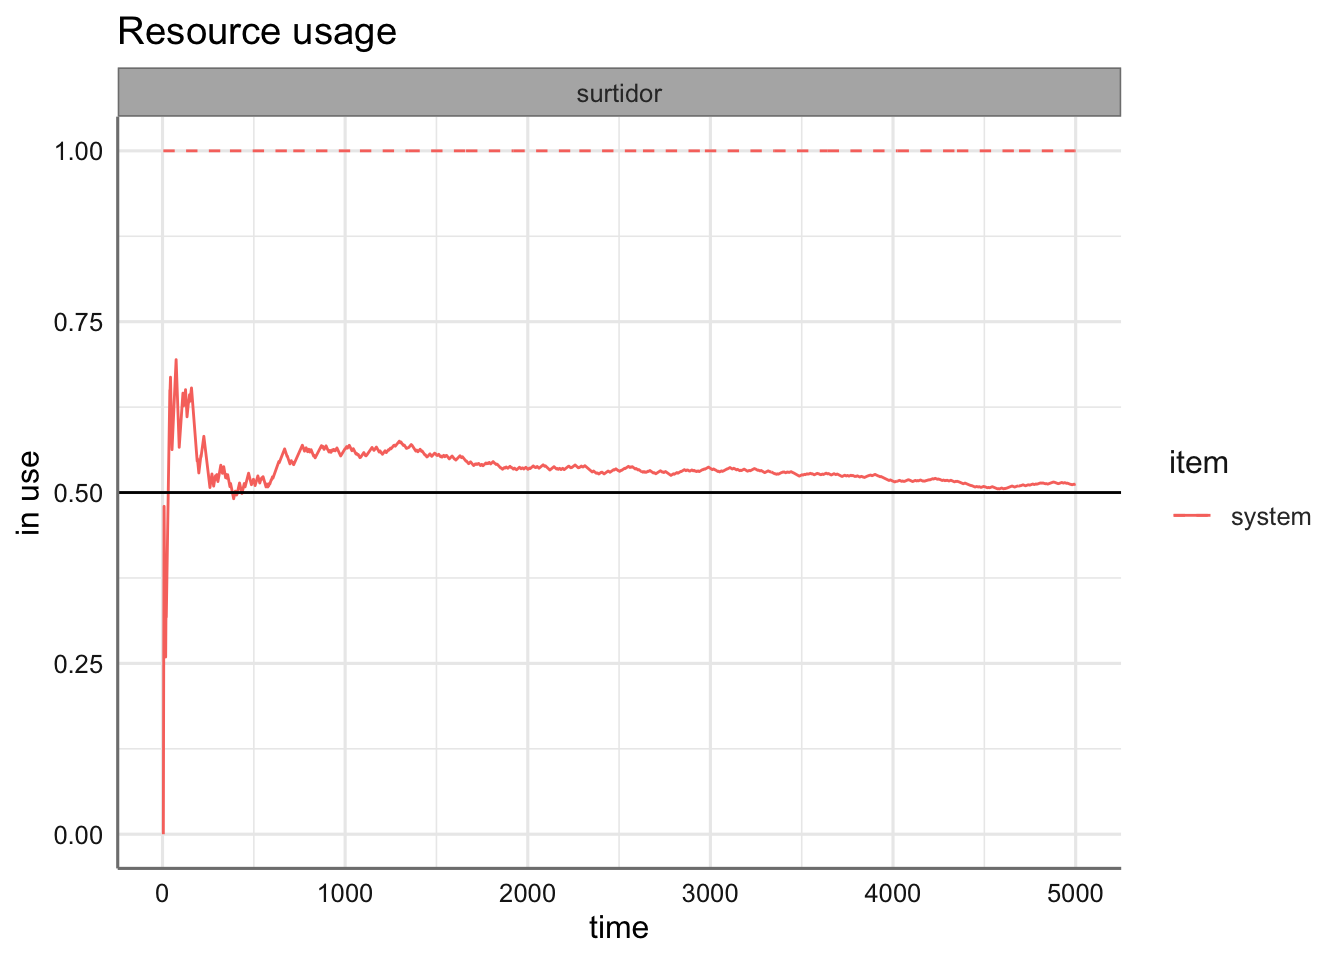
\includegraphics[width=0.95\linewidth]{07-simmer_files/figure-latex/unnamed-chunk-41-2} \end{center}

\hypertarget{referencias}{%
\section{Referencias}\label{referencias}}

Bache SM, Wickham H (2014). magrittr: A Forward-Pipe Operator for R. R package version 1.5. Available at \url{https://CRAN.R-project.org/package=magrittr}.

Banks J (2005). Discrete-Event System Simulation. Prentice-Hall International Series in Industrial and Systems Engineering. Pearson Prentice Hall.

Canadilla, P. (2019). Analysis of Queueing Networks and Models. Package `queueing'. Available at \url{https://cran.r-project.org/web/packages/queueing/}.

Chubaty AM, McIntire EJB (2019). SpaDES: Develop and Run Spatially Explicit Discrete Event Simulation Models. R package version 2.0.3. Available at \url{https://CRAN.R-project.org/package=SpaDES}.

Ebert A (2018). queuecomputer: Computationally Efficient Queue Simulation. R package version 0.8.3. Available at \url{https://CRAN.R-project.org/package=queuecomputer}.

Ebert A, Wu P, Mengersen K, Ruggeri F (2017). Computationally Efficient Simulation of Queues: The R Package queuecomputer.'' arXiv:1703.02151. ArXiv.org E-Print Archive. Available at \url{http://arxiv.org/abs/1703.02151}.

FishyOperations in R-Bloggers (2016). Simulating queueing systems with simmer. Available at \url{https://www.r-bloggers.com/2016/04/simulating-queueing-systems-with-simmer/}.

Kendall DG (1953). Stochastic Processes Occurring in the Theory of Queues and their Analysis by the Method of the Imbedded Markov Chain.'' The Annals of Mathematical Statistics, 24(3), 338-354. Available at \url{https://doi.org/10.1214/aoms/1177728975}.

Lauwens B (2017). SimJulia.jl: Combined Continuous-Time / Discrete-Event Process Ori-ented Simulation Framework Written in Julia. Julia package version 0.5. Available at \url{https://github.com/BenLauwens/SimJulia.jl}.

Law AM, Kelton WD (2000). Simulation Modeling and Analysis. McGraw-Hill Series in
Industrial Engineering and Management Science. McGraw-Hill.

Pidd M (1988). Computer Simulation in Management Science. John Wiley \& Sons.

Shannon RE (1975). Systems Simulation: The Art and Science. Prentice-Hall.

Team SimPy (2017). SimPy: Discrete-Event Simulation for Python. Python package version
3.0.9. Available at \url{https://simpy.readthedocs.io/en/stable}.

Ucar, I., Smeets, B., Azcorra, A. (2019). ``simmer: Discrete-Event
Simulation for R.'' \emph{Journal of Statistical Software}, \emph{90}(2), 1-30.
Available at \url{https://doi.org/10.18637/jss.v090.i02}.

Ucar, I., Smeets, B. (2019a). simmer: Discrete-Event Simulation for R. R package version 4.3.0. Available at \url{https://CRAN.R-project.org/package=simmer}.

Ucar, I., Smeets, B. (2019b). simmer.plot: Plotting Methods for simmer. R package version 0.1.15. Available at \url{https://CRAN.R-project.org/package=simmer.plot}.

Ucar, I., Smeets, B. (2020c) simmer: DES for R. Available at \url{https://r-simmer.org/}. Documentation is available at \url{https://r-simmer.org/reference/}.

Ucar, I. (2020a). Queueing systems, in simmer: DES for R. Available at \url{https://r-simmer.org/articles/simmer-06-queueing.html}.

Ucar, I. (2020b). Continuous-Time Markov Chains, in simmer: DES for R. Available at \url{https://r-simmer.org/articles/simmer-07-ctmc.html}.

  \bibliography{book.bib,packages.bib}

\end{document}
